\documentclass[letterpaper,11pt]{report}
\usepackage{float,captdef,multicol}
\usepackage{amssymb,amsmath,amsfonts,fancybox}
\usepackage[activeacute,spanish,es-tabla]{babel}
\usepackage[utf8]{inputenc}
\usepackage[colorlinks]{hyperref}
\usepackage{graphicx}
\usepackage{cancel}
\usepackage{marginnote}

\renewcommand*{\marginnotevadjust}{-0.1cm}
\renewcommand*{\marginfont}{\footnotesize}
\usepackage[right=4.5cm,left=2cm,top=3cm,bottom=3.0cm]{geometry}

%\usepackage[notref]{showkeys} % muestra los labels de las referencias.

\spanishdecimal{.}


\begin{document}

\sffamily

\thispagestyle{empty}
\begin{center}

\

\vspace{6.5cm}

\rule{15cm}{0.1cm}

\vspace{1.5cm}

{\huge \textsc{\textbf{Teor'ia General de la Relatividad \\ \ \\ T'opicos en Relatividad General}}}

\vspace{1.5cm}

\rule{15cm}{0.1cm}

\vspace{1.5cm}

Versi'on del \today

\end{center}


\newpage
\thispagestyle{empty}
\ \\
\newpage
\setcounter{page}{1}
\pagenumbering{roman}

\pagestyle{plain}
\chapter*{Prefacio}
\addcontentsline{toc}{chapter}{Prefacio}
\bigskip
\bigskip
\bigskip
\bigskip
\bigskip
\bigskip



Este apunte ha sido escrito principalmente por \href{https://twitter.com/gfrubi}{G. Rubilar}, con contribuciones de J. Cris'ostomo, O. Fuentealba (cap. \ref{cap:Kerr}), N. Ibarra, F. Izaurieta, N. Merino (cap. \ref{cap:tensores}), J. Moya (cap. \ref{cap:cosmo}), P. Mu\~noz (cap. \ref{chap:eq_newton} y \ref{cap:Eq-Rel}),  A. P'erez (cap. \ref{cap:tensores}), T. Ramos (cap. \ref{cap:gravito}), E. Rodriguez y O. Valdivia.


\bigskip
\bigskip
\bigskip
\bigskip
\bigskip
\bigskip



Esta obra ha sido publicada bajo una \href{https://github.com/gfrubi/RG/blob/master/LICENSE}{licencia GPL v3}. El c'odigo fuente (pdf)\LaTeX, as'i como las figuras en formato editable est'an disponibles en el \href{https://github.com/gfrubi/RG}{repositorio GitHub del proyecto}.


\bigskip
\bigskip
\bigskip

\bigskip
\bigskip
\bigskip




\emph{\textquotedblleft ...As\'i, nosotros los mortales, somos
inmortales en lo que creamos en com\'un."}

\begin{flushright}
Albert Einstein.
\end{flushright}
\newpage

\tableofcontents
\pagenumbering{arabic}
\setcounter{page}{1}
\chapter{Motivaciones para RG: Relatividad Especial y Gravitaci'on newtoniana}
\section{Distribuci'on de energ'ia y mom'entum de la materia: tensor de energ'ia-mom'entum}

Para un resumen de las definiciones b'asicas, la notaci'on y convenciones usadas en la teor'ia de la mec'anica y electrodin'amica relativista, vea los apuntes de Electrodin\'amica (II) \cite{7}.

En la teor'ia newtoniana de la gravitaci'on la \textit{masa} de los cuerpos es la fuente del campo gravitacional. Desde el punto de vista de una descripci'on de un sistema como un \textit{continuo}, la distribuci'on espacial y el movimiento de su masa es caracterizada por 4 cantidades: la densidad de masa $\rho$ y (las tres componentes de) la densidad de corriente de masa\footnote{Si el sistema est'a constituido de una distribuci'on de densidad $\rho$ que se mueve con velocidad $\vec{v}$, entonces $\vec{J}=\rho\vec{v}$.} $\vec{J}$. En la teor'ia de RE, por otro lado, la masa de los cuerpos no es m'as que una componente de la energ'ia de 'estos: el concepto de masa es reemplazado por el de energ'ia (no existe ley de conservaci'on de la masa de un sistema, sino s'olo de la energ'ia total, etc.). M'as a'un, la energ'ia es ``s'olo'' una componente del 4-mom'entum de un cuerpo. Los valores de las componentes del 4-mom'entum, y por lo tanto de la energ'ia y del mom'entum lineal, se ``mezclan'' al describir un sistema desde distintos SRI's (el 4-mom'entum es un 4-vector bajo TL's). Por todo esto, es natural suponer que en una teor'ia relativista de la gravitaci'on las fuentes del campo gravitacional est'en descritas por la distribuci'on de energ'ia y mom'entum en el espacio(tiempo) y sus flujos\footnote{Es decir, densidad de energ'ia, densidad de flujo de energ'ia, densidad de mom'entum y densidad de flujo de mom'entum.}. Todas estas cantidades quedan condensadas en el \textit{tensor energ'ia-mom'entum de un sistema}.

Las componentes del tensor de energ'ia-mom'entum\footnote{De acuerdo a nuestras convenciones este tensor tiene unidades de \textit{densidad de energ'ia}, es decir, energ'ia por unidad de volumen o, equivalentemente, de \textit{presi'on}.} $T^{\mu\nu}$ est'an relacionadas con las densidades y flujos de energ'ia y mom'entum, de acuerdo a
\begin{equation}
 T^{00}(x)=u(x), \qquad T^{0i}(x)=\frac{1}{c}S^i(x), \qquad T^{i0}(x)=c\,\pi^i(x), \qquad T^{ij}(x)=p^{ij}(x),
\end{equation}
donde $u$ es la \textit{densidad de energ'ia} (energ'ia por unidad de volumen), $S^i$ la \textit{densidad de flujo de energ'ia} (energ'ia por unidad de tiempo y superficie), $\pi^i$ la \textit{densidad de mom'entum} (mom'entum por unidad de volumen) y $p^{ij}$ el \textit{tensor de tensiones} (mom'entum por unidad de tiempo y superficie).

El \textit{4-mom'entum total del sistema}, contenido en un volumen $V$ en un instante dado, es entonces la integral
\begin{equation}
p^\mu=\frac{1}{c}\int_V T^{\mu 0}\,dV \label{pmTmn}
\end{equation}
o, equivalentemente, la energ'ia y el mom'entum adoptan la forma
\begin{equation}
E=\int_V u\,dV, \qquad P^i=\int_V \pi^i\,dV.
\end{equation}
Si el sistema est'a \textit{aislado}, de modo que su energ'ia y mom'entum se conserven, se satisface 
\begin{equation}
 \partial_\nu T^{\mu \nu}=0
\end{equation}
que, en virtud de las identificaciones anteriores, es equivalente a las usuales ``ecuaciones de continuidad'' para la energ'ia y el mom'entum:
\begin{equation}
 \partial_tu+\partial_iS^i=0, \qquad \partial_t \pi^i+\partial_jp^{ij}=0.
\end{equation}


\subsection{Campo electromagn'etico}
El campo electromagn'etico posee y transporta energ'ia y mom'entum. El respectivo tensor de energ'ia-mom'entum del campo electromagn'etico en el vac'io es dado por
\begin{equation}
\boxed{T_\text{em}^{\mu\nu}:=\frac{1}{\mu_0}\left(  F^{\mu\lambda}F_\lambda^{\ \nu}+\frac{1}{4}F_{\rho\sigma}F^{\rho\sigma}\eta^{\mu\nu} \right).}  \label{temsimSI}
\end{equation}
Puede verificarse que las densidades de energ'ia, mom'entum y sus flujos est'an dados por las cantidades apropiadas definidas en electrodin'amica:
\begin{align}
u &:= \frac{1}{2}\left(\varepsilon_0\vec{E}^2+\frac{1}{\mu_0}\vec{B}^2\right),\label{uTheta}\\
S^i &:= \frac{1}{\mu_0}\left(\vec{E}\times\vec{B}\right)^i=c^2\pi^i, \label{STheta}\\
T^{ij} &:= \frac{1}{2}\left(\varepsilon_0\vec{E}^2+\frac{1}{\mu_0}\vec{B}^2\right)\delta_j^i-\varepsilon_0 E^i E^j -\frac{1}{\mu_0}B^i B^j , \label{TTheta}
\end{align}
Para mayores detalles, ver \cite{7}.


\subsection{Fluido perfecto}
Consideramos ahora un fluido con estructura interna descrita por una \textit{presi'on
is'otropa} $p$. 'Esta est'a definida respecto al SRI com'ovil $K'$ con un elemento de fluido dado, ubicado en el evento $x$, de modo que
\begin{eqnarray}
T'^{00}(x)&=&\epsilon(x) , \label{t00c}\\
T'^{0i}(x) &=&0, \label{t0ic}\\
T'^{i0}(x) &=&0, \label{ti0c}\\
T'^{ij}(x) &=&p(x)\,\delta^{ij} .\label{tijc}
\end{eqnarray}

La componente en (\ref{t00c}) es la \textit{densidad propia de energ'ia} (es decir, $\epsilon(x)\,dV'$ es la energ'ia del sistema contenida en el elemento de volumen $dV'$, en el SRI instant'aneamente com'ovil con el fluido en el evento $x$), que a menudo se expresa en t'erminos de la \textit{densidad propia de masa} $\rho(x)$, definida por $\rho(x):=\epsilon(x)/c^2$. Las componentes
mixtas (\ref{t0ic}) y (\ref{ti0c}) son nulas puesto que suponemos que en el sistema com'ovil \textit{la distribuci'on microsc'opica es is'otropa}, por lo que no existe una direcci'on preferente para el flujo de energ'ia ni para la densidad de mom'entum. Finalmente las componentes espaciales
en (\ref{tijc}) son diagonales puesto que \textit{suponemos que en un fluido
perfecto la fuerza sobre cada elemento de superficie es normal a esta
superficie}, de modo que $T^{ij}dS^j=T^{ij}\,\hat{n}^j\,dS=p\,\hat{n}^i dS$ y que $p>0$ corresponde a un fluido que tiende a expandirse.

A partir del tensor de energ'ia-mom'entum para un fluido perfecto en su sistema local com'ovil, encontraremos la expresi'on general respecto a cualquier
otro SRI por medio del boost de Lorentz apropiado. Para esto usaremos los resultados y convenciones contenidos en \cite{7}. Si la TL es denotada como $x'^\mu=\Lambda^\mu_{\ \nu}x^\nu$ y $v^i=c\beta^i$ es la velocidad de $K'$ respecto a $K$ entonces
\begin{equation}
 \Lambda^0_{\ 0}=\gamma, \qquad \Lambda^i_{\ 0}=\Lambda^0_{\ i}=-\gamma\beta^i, \qquad \Lambda^i_{\ j}=\delta^i_j
+\frac{(\gamma-1) }{\beta^2}\beta^i\beta^j .
\end{equation}
Por otro lado el tensor buscado $T^{\mu\nu}$ est'a relacionado con $T'^{\mu\nu}$ por medio de
\begin{eqnarray}
T^{\mu\nu}&=&(\Lambda^{-1})^\mu_{\ \lambda}(\Lambda^{-1})^\nu_{\ \rho}T'^{\lambda\rho}
\\
&=& (\Lambda^{-1})^\mu_{\ 0}\Lambda^\nu_{\ 0}T'^{00}+(\Lambda^{-1})^\mu_{\
i}\Lambda^\nu_{\ j}T'^{ij}\\
&=& (\Lambda^{-1})^\mu_{\ 0}(\Lambda^{-1})^\nu_{\ 0}\rho c^2+p(\Lambda^{-1})^\mu_{\
i}(\Lambda^{-1})^\nu_{\ j}\delta^{ij}.
\end{eqnarray}
Las componentes de la matriz $(\Lambda^{-1})$ est'an dadas por
\begin{equation}
(\Lambda^{-1})^0_{\ 0}=\gamma, \qquad (\Lambda^{-1})^i_{\ 0}=(\Lambda^{-1})^0_{\ i}=+\gamma\beta^i, \qquad (\Lambda^{-1})^i_{\ j}=\delta^i_j
+\frac{(\gamma-1) }{\beta^2}\beta^i\beta^j .
\end{equation}
Por lo tanto, obtenemos que
\begin{eqnarray}
T^{00}&=& (\Lambda^{-1})^0_{\ 0}(\Lambda^{-1})^0_{\ 0}\rho c^2+p(\Lambda^{-1})^0_{\ i}(\Lambda^{-1})^0_{\ j}\delta^{ij} \\
&=& \gamma^2\rho c^2+p\gamma^2\beta^i\beta^j\delta^{ij} \\
&=& \gamma^2\rho c^2+p\gamma^2\beta^2 .
\end{eqnarray}

Vemos que en el contexto de la teor'ia Especial de la Relatividad \textit{la presi'on de un fluido en movimiento aporta a su densidad de energ'ia}\footnote{En su generalizaci'on a la teor'ia General de la Relatividad, este hecho tiene importantes consecuencias, por ejemplo, para el an'alisis de estabilidad (y colapso) estelar.}. Adem'as,
\begin{eqnarray}
T^{0i}&=& (\Lambda^{-1})^0_{\ 0}(\Lambda^{-1})^i_{\ 0}\rho c^2+p\,(\Lambda^{-1})^0_{\ j}(\Lambda^{-1})^i_{\ k} \delta^{jk} \\
&=& \gamma^2\beta^i\rho c^2 +p\gamma\beta^j\left(\delta^i_k
+\frac{1}{\beta^2}\beta^i\beta^k(\gamma-1) \right) \delta^{jk} \\
&=& \gamma^2\beta^i\rho c^2 +p\gamma\left(\beta^i +\beta^i(\gamma-1) \right)
\\
&=& \gamma^2\beta^i\rho c^2 +p\gamma^2\beta^i,
\end{eqnarray}
y $T^{i0}=T^{0i}$. Note adem'as que $T^{0i}\neq T^{00}\beta^i$ cuando $p\neq 0$. Finalmente,
\begin{eqnarray}
T^{ij}&=& (\Lambda^{-1})^i_{\ 0}(\Lambda^{-1})^j_{\ 0}\rho c^2+p\,(\Lambda^{-1})^i_{\ k}(\Lambda^{-1})^j_{\ l}\delta^{kl} \\
&=&\gamma^2\beta^i\beta^j\rho c^2+ p\left(\delta^i_k+
\frac{1}{\beta^2}\beta^i\beta^k(\gamma-1) \right)\left(\delta^j_l
+\frac{1}{\beta^2}\beta^j\beta^l(\gamma-1) \right)\delta^{kl} \\
&=&\gamma^2\beta^i\beta^j\rho c^2+p\left(\delta^{ij}
+\frac2{\beta^2}\beta^i\beta^j(\gamma-1)
+\frac{1}{\beta^2}\beta^i\beta^j(\gamma-1)^2\right) \\
&=&\gamma^2\beta^i\beta^j\rho c^2+p\left(\delta^{ij}
+\frac{1}{\beta^2}\beta^i\beta^j(\gamma^2-1)\right) \\
&=&\gamma^2\beta^i\beta^j\rho c^2+p\left(\delta^{ij}
+\gamma^2\beta^i\beta^j\right).
\end{eqnarray}
Puede verificarse f'acilmente que 'estas son precisamente las componentes de
\begin{equation}\label{temfp}
\boxed{T_{\rm fp}^{\mu\nu}=\left( \rho +\frac{p}{c^2}\right) u^\mu
u^\nu-p\,\eta^{\mu\nu}.}\marginnote{energ'ia-mom'entum fluido perfecto}
\end{equation}

La expresi'on (\ref{temfp}) constituye por tanto la expresi'on covariante del tensor de energ'ia-mom'entum de un fluido perfecto, caracterizado por su densidad propia de masa $\rho$, y su presi'on is'otropa $p$, movi'endose con 4-velocidad $u^\mu$. Estas tres cantidades son, en general, dependientes de la posici'on y del tiempo. En t'erminos de la densidad propia de energ'ia, $\epsilon$, tenemos:
\begin{equation}\label{temfpu}
\boxed{T_{\rm fp}^{\mu\nu}=\left(\epsilon +p\right)\frac{u^\mu}{c}
\frac{u^\nu}{c}-p\,\eta^{\mu\nu}.}\marginnote{energ'ia-mom'entum fluido perfecto}
\end{equation}
\subsection{Fluido simple (polvo)}

El caso particular de un fluido simple, es decir, sin presi'on, describe la situaci'on en que el sistema est'a constituido por  un conjunto de part'iculas \textit{no interactuantes movi'endose todas con la misma velocidad} en un elemento de volumen dado (``polvo''). El tensor energ'ia-mom'entum se reduce entonces a:
\begin{equation}
\boxed{T_{\rm polvo}^{\mu\nu}(x)=\rho\, u^\mu u^\nu.}
\end{equation}

Las respectivas densidades de energ'ia, de flujo de energ'ia, de mom'entum y el
tensor de tensiones est'an dadas en este caso por:
\begin{eqnarray}
u&=&\rho \gamma^2 c^2, \\ 
S^i&=&\rho \gamma^2c^2v^i=u\,v^i, \\ 
{\pi}^i&=&\rho \gamma^2v^i =\frac{u}{c^2}v^i, \\ 
p^{ij} &=&\rho \gamma^2 v^i v^j=\pi^iv^j.
\end{eqnarray}
Note que para este tipo de sistema se verifica que los respectivos flujos $S^i$ y $p^{ij}$ tienen la forma esperada de producto de la respectiva densidad (``transportada'') y la velocidad de cada elemento de fluido (``a la que es transportada''), tal como ocurre por ejemplo para una distrubuci'on de carga de densidad $\rho_{\rm c}$ movi'endose con velocidad $\vec{v}_{\rm c}$, para la cual la densidad de corriente es dada por $\vec{J}_{\rm c}=\rho_{\rm c}\vec{v}_{\rm c}$.

\section{Ley de Gravitaci'on universal}
En la teor'ia newtoniana la fuerza gravitacional de una masa muy peque\~na (``puntual'') $m_1$ sobre otra masa (tambi'en muy peque\~na) $m_2$
est'a dada por la ley de gravitaci'on de Newton ($1687$),
\begin{equation}
\vec{F}_{1\rightarrow 2}=-G\frac{m_1m_2}{|\vec{r}|^2}\frac{\vec{r}}{|\vec{r}|},
\end{equation}
donde $G$ es la constante de gravitaci'on (de Cavendish, medida por primera vez en 1897). Su valor, de acuerdo a las mediciones actuales, es\footnote{Ver por ejemplo, \url{http://www.codata.org}.}
\begin{equation}
G\stackrel{\rm SI}{=}(6,674 28\pm 0.000 67)\times 10^{-11}\, m^3kg^{-1}s^{-2}.
\end{equation}
El vector $\vec{r}:=\vec{x}_2-\vec{x}_1$ apunta desde $m_1$ hasta $m_2$, ver figura \ref{lguN}. De acuerdo al principio de acci'on y reacci'on (tercera ley de Newton),
tenemos que $\vec{F}_{1\rightarrow 2}=-\vec{F}_{2\rightarrow 1}$.
\begin{center}
\begin{figure}[H]
\centerline{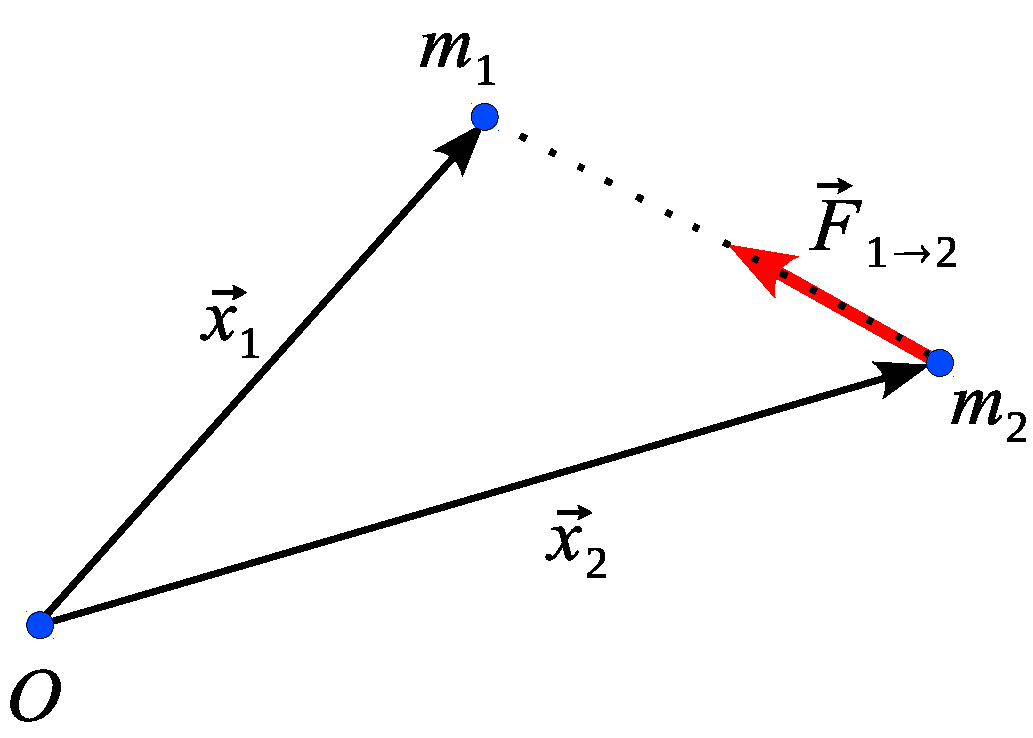
\psfig{file=fig/fig-ley-gravitacion-Newton.pdf,height=4cm,angle=0}}
\caption{Ley de gravitaci'on universal de Newton.}
\label{lguN}
\end{figure}
\end{center}
El \textit{campo gravitacional} $\vec{g}$ es definido como la fuerza por unidad de masa
que experimenta una masa de prueba. Por tanto, el campo gravitacional en la posici'on $\vec{x}_2$ generado por una masa (muy peque\~na) $m_1$ es
\begin{equation}
\vec{g}_1(x_2):=\frac{\vec{F}_{1\to 2}}{m_2}=-G\frac{m_1}{|\vec{r}|^2}\frac{\vec{r}}{|\vec{r}|}.
\end{equation}
En el caso anterior, es posible distinguir entre la masa $m_1$ que
\textit{genera} el campo gravitacional, que llamamos \textit{masa gravitacional
activa}, y la masa $m_2$ de la part'icula que sobre la cual act'ua la fuerza, que
llamaremos \textit{masa gravitacional pasiva}.

Por el \textit{principio} de superposici'on, el campo gravitacional generado por una distribuci'on continua de masa, caracterizada por su densidad de masa $\rho(\vec{x})$ ser'a de la forma
\begin{equation}
\vec{g}(\vec{x})=-G\int_V\frac{\rho(\vec{x}')(\vec{x}-\vec{x}')}{|\vec{x}-\vec{x}'|^3}dV'.
\end{equation}
Como consecuencia, el campo gravitacional es siempre irrotacional,
\begin{equation}
\vec{\nabla}\times\vec{g}=\vec{0},
\end{equation}
y puede derivarse a partir de un \textit{potencial gravitacional} $\phi$, de modo
que
\begin{equation}
\boxed{\vec{g}(x)=-\vec{\nabla}\phi(x),}
\end{equation}
donde
\begin{equation}
\phi(\vec{x}):=-G\int_V\frac{\rho(\vec{x}')}{|\vec{x}-\vec{x}'|}dV'+\text{cte}.
\end{equation}
Este potencial satisface la \textit{ecuaci'on de Poisson},
\begin{equation}\marginnote{Ecuaci'on de Poisson}
\boxed{\nabla^2\phi=4\pi G \rho,} \label{Poisson}
\end{equation}
o equivalentemente, el campo gravitacional satisface la ecuaci'on (``de Gauss")
\begin{equation}
\vec\nabla\cdot\vec{g}=-4\pi G \rho, \label{gaussg}
\end{equation}
que relaciona los \textit{gradientes} del campo gravitacional con la distribuci'on de masa, descrita por la densidad $\rho(\vec{r})$, que lo genera.

Si bien la ecuaci'on (\ref{Poisson}) es una ecuaci'on para el campo $\phi$, en el
contexto newtoniano el campo gravitacional no es un genuino \textit{campo
din'amico}, es decir, no contiene grados de libertad independientes, ya que
'este queda determinado (para condiciones de borde dadas) 'unicamente por la
densidad de masa $\rho$. En otras palabras, la teor'ia newtoniana de la
gravitaci'on es una teor'ia de \textit{acci'on a distancia}. De acuerdo a este modelo, si se removiese la fuente del campo ($\rho\rightarrow 0$) entonces el campo gravitacional desaparecer'ia \textit{instant'aneamente} en todo punto. El mismo Newton estaba bastante preocupado por este hecho. Claramente, esta propiedad es \textit{incompatible} con los postulados b'asicos de la teor'ia de Relatividad Especial.

\section{Masa inercial y masa gravitacional}
Una caracter'istica especial de la interacci'on gravitacional es que, hasta donde hemos podido observar, la aceleraci'on de un cuerpo que cae libremente en un campo gravitacional dado \textit{no depende de su masa sino s'olo de su posici'on} en el campo gravitacional. En el contexto newtoniano esto puede describirse a trav'es de la igualdad entre la \textbf{masa inercial} y la \textbf{masa gravitacional} de \textit{todo cuerpo}.

En este contexto, la \textbf{masa inercial} de un cuerpo, $\stackrel{\rm iner}{m}$, es definida como aquella cantidad que mide la resistencia de 'este a cambiar su estado de movimiento, de acuerdo a la segunda ley de Newton:
\begin{equation}\label{2ln}
\vec{F}=\stackrel{\rm iner}{m}\frac{d^2\vec{x}}{dt^2}.
\end{equation}
Esta masa puede ser determinada por medio de experimentos ``no-gravitacionales'', es decir, que no involucran la interacci'on gravitacional. Por ejemplo, puede determinarse la masa inercial de un cuerpo comparando su frecuencia de oscilaci'on $\omega$ con la frecuencia de oscilaci'on de un cuerpo de referencia $\omega_{\rm ref}$) cuando ambos son unidos alternativamente a un mismo resorte, de modo que se produzca una oscilaci'on horizontal. En este caso (suponiendo la ley de Hooke) se cumple que $\stackrel{\rm iner}{m}/\stackrel{\rm iner}{m}_{\rm ref}=\omega_{\rm ref}^2/\omega^2$.

Por otro lado, se define la \textbf{masa gravitacional}, $\stackrel{\rm grav}{m}$, de un cuerpo como la cantidad que mide la magnitud de la fuerza que este cuerpo experimenta al estar en una regi'on del espacio con campo gravitacional $\vec{g}$:
\begin{equation}\label{fg}
\vec{F}_{\rm grav}=\stackrel{\rm grav}{m}\vec{g}=-\stackrel{\rm grav}{m}\vec\nabla\phi.
\end{equation}
A partir de (\ref{2ln}) y (\ref{fg}) obtenemos que la aceleraci'on de un cuerpo debido a un campo gravitacional $\vec{g}$ es dado por
\begin{equation}\label{amimg}
\frac{d^2\vec{x}}{dt^2}=\left(\frac{\stackrel{\rm grav}{m}}{\stackrel{\rm iner}{m}}\right)\vec{g}.
\end{equation}
Esta expresi'on es an'aloga a la que determina la aceleraci'on de un cuerpo cargado en presencia de un campo el'ectrico externo:
\begin{equation}\label{aqE}
\frac{d^2\vec{x}}{dt^2}=\left(\frac{q}{\stackrel{\rm iner}{m}}\right)\vec{E}.
\end{equation}
En este sentido, la masa gravitacional es el an'alogo gravitacional a la carga el'ectrica (es decir, es la ``carga gravitacional'').


\subsection{Universalidad de la interacci'on gravitacional, Principio de Equivalencia D'ebil}

La experiencia muestra que la interacci'on electrost'atica causa, incluso en presencia de un mismo campo el'ectrico, que cuerpos diferentes aceleren en forma diferente. Esto se describe, de acuerdo a (\ref{aqE}), diciendo que distintos cuerpos poseen distintos valores de la relaci'on carga-masa (inercial) $q/m$. Existen cuerpos donde esta relaci'on es positiva, negativa, o cero. En contraste, la interacci'on gravitacional \textit{parece} (de acuerdo a todas observaciones realizadas hasta hoy) tener la propiedad 'unica que \textit{todos} los cuerpos aceleran en la \textit{misma} direcci'on y con la \textit{misma} magnitud en un campo gravitacional dado. De acuerdo a (\ref{amimg}), esto requiere que el cuociente entre la masa inercial y gravitacional de todo cuerpo sea una constante universal (es decir, que tenga siempre el mismo valor, independiente del cuerpo). Por simplicidad, usualmente se eligen las unidades de $\stackrel{\rm grav}{m}$ (o, equivalentemente, de la constante gravitacional $G$) tal que esta \textit{universalidad de la interacci'on gravitacional} implique que
\begin{equation}
\boxed{\stackrel{\rm iner}{m}=\stackrel{\rm grav}{m}.}
\end{equation}
En este caso, (\ref{amimg}) se reduce a
\begin{equation}\label{ag}
\frac{d^2\vec{x}}{dt^2}=\vec{g}
\end{equation}
\textit{para todo cuerpo}.

Si el \textit{postulado} de universalidad de la interacci'on gravitacional o, en otras palabras, de la igualdad de masa inercial y gravitacional, es \textit{siempre} v'alido entonces la trayectoria de los cuerpos sometidos (s'olo) a la acci'on de la gravedad es independiente del cuerpo (de su carga, composici'on, temperatura, color, etc.) y s'olo depende del campo gravitacional en el que se encuentra (determinado por los otros cuerpos en el sistema) y de la posici'on y velocidad inicial de 'este. La suposici'on que las trayectorias de los cuerpos sometidos a la acci'on de la gravedad son realmente id'enticas (dadas las mismas condiciones iniciales) es usualmente llamado \textbf{Principio de Equivalencia D'ebil} (PED). Lo importante es que la validez del PED o, equivalentemente, de la universalidad de la aceleraci'on debido a la gravedad, o de la igualdad de las masas inerciales y gravitacionales, son caracter'isticas distintivas de la interacci'on gravitacional que se han obtenido a partir de la generalizaci'on de \textit{observaciones}, y que pueden (y deben!) ser testeadas experimentalmente. Hasta ahora, toda la evidencia observacional respalda al PED, siendo verificado con precisiones que restringen las posibles \textbf{desviaciones relativas de la aceleraci'on}, y por lo tanto la diferencia relativa del cuociente $\stackrel{\rm iner}{m}/\stackrel{\rm grav}{m}$ entre dos cuerpos (``1'' y ``2'')
\begin{equation}
\frac{\Delta a}{a}=\frac{\left(\stackrel{\rm iner}{m}/\stackrel{\rm grav}{m}\right)_2-\left(\stackrel{\rm iner}{m}/\stackrel{\rm grav}{m}\right)_1}{\left(\stackrel{\rm iner}{m}/\stackrel{\rm grav}{m}\right)_1},
\end{equation}
a ser menores que una parte en $10^{13}$. Para m'as detalles, ver \cite{Will06}-\cite{STEP}.
Estas observaciones abarcan desde los experimentos originales de Galileo usando p'endulos, planos inclinados, etc. hasta los m'as modernos y precisos experimentos con sat'elites e incluso neutrones \cite{Koester76} y electrones. El PED tambi'en ha sido testeado con 'atomos, usando t'ecnicas de interferometr'ia at'omica, ver \cite{Zhou15} y las referencias ah'i citadas. Recientemente, se han reportado experimentos que testean el PED con 'atomos con distintas orientaciones de su spin, ver \cite{Duan16}.

Como veremos m'as adelante, la teor'ia general de la relatividad de Einstein \textit{supone} como ingrediente crucial para su construcci'on el PED\footnote{de hecho se postula una versi'on generalizada y a'un m'as demandante, el as'i llamado ``principio de equivalencia fuerte'' (PEF).}. Por esta raz'on existe continuo inter'es en poner a prueba este principio, y mejorar cada vez m'as la precisi'on con la que se ha verificado su validez.

El siguiente gr'afico resume los resultados de m'ultiples experimentos modernos que determinan cotas m'aximas para las aceleraciones relativas de distintos cuerpos sometidos a la acci'on de la gravedad, junto con el a\~no en que fueron realizados los experimentos.
\begin{center}
\begin{figure}[H]
\centerline{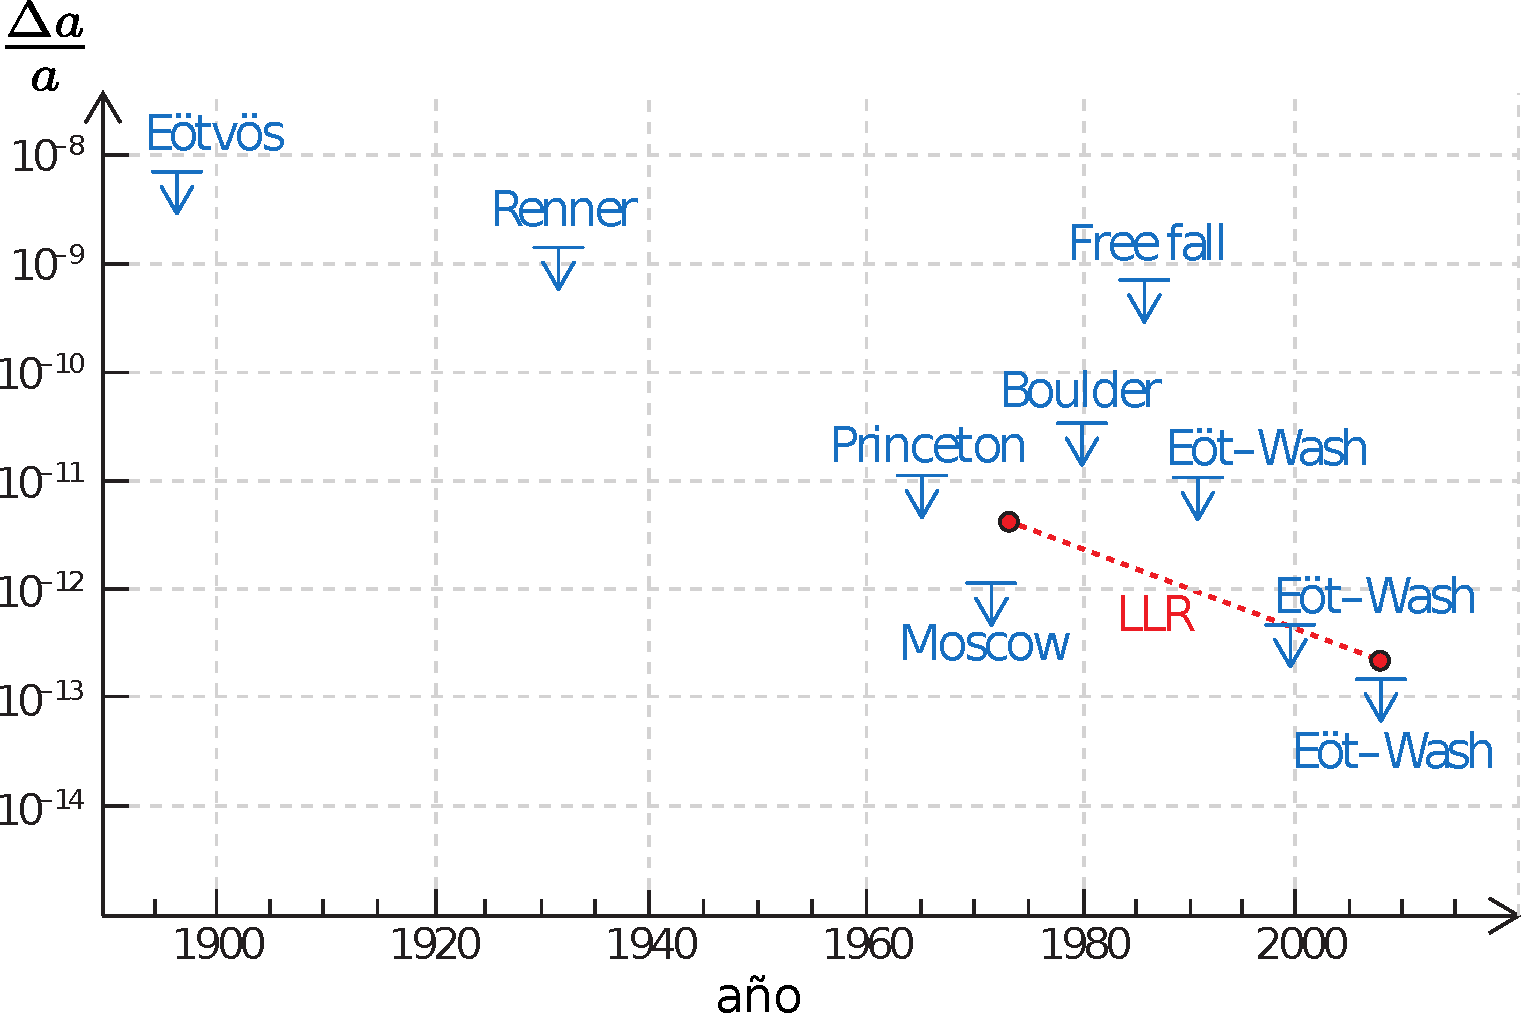
\psfig{file=fig/fig-tests-PED.pdf,height=5cm,angle=0}}
\caption{L'imites a posibles violaciones del PED. Figura adaptada a partir de la original en \cite{Turyshev08}.}
\label{fig:equiv1}
\end{figure}
\end{center}

\section{Fuerzas de marea}
%Tal como hemos visto, un indicador de la presencia de campo gravitacional no nulo es la \textit{aceleraci'on relativa} entre distintos SRLI's. 
En el contexto newtoniano, se usa el t'ermino \textbf{fuerzas de marea} para describir el efecto de la \textit{inhomogeneidad} de un campo gravitacional, que genera diferencias en la aceleraci'on de la materia en distintas partes de un sistema. Considere el caso de un campo gravitacional generado por una distribuci'on compacta de masa (ver, por ejemplo, la figura \ref{fig:SRLI}). Debido a las inhomogeneidades del campo gravitacional, dos peque\~nas masas de prueba inicialmente en reposo caer'an hacia el centro de fuerzas, acerc'andose entre ellas. Similarmente, una gota de agua inicialmente esf'erica tender'a a deformarse a una forma elipsoidal debido a que la fuerza gravitacional en su parte inferior (m'as cerca del centro de fuerzas) es mayor que en la parte superior, que est'a a una distancia mayor de la fuente.

Si la distancia entre las dos masas de prueba es \emph{suficientemente peque\~na}, podemos encontrar una expresi'on expl'icita simple para su aceleraci'on relativa. Considere que las posiciones de estas masas son $\vec{x}$ y $\vec{x}+\delta\vec{x}$.
Podemos entonces, a primer orden en $\delta\vec{x}$, escribir:
\begin{equation}
a_i(\vec{x}+\delta\vec{x})=a_i(\vec{x})+\delta x^j\partial_j a_i(\vec{x}).
\end{equation}
Esta aproximaci'on es buena si $|\delta\vec{x}|\ll |a_i|/|\partial_j
a_i|$. Definimos el \textbf{tensor de mareas} $K_{ij}$ por
\begin{equation}\marginnote{Tensor de Mareas}
K_{ij}(\vec{x}):=-\partial_j a_i(\vec{x}),
\end{equation}
(el signo negativo es convencional) de modo que
\begin{equation}
\delta a_i:=a_i(\vec{x}+\delta\vec{x})-a_i(\vec{x})=- K_{ij}\delta x^j.
\end{equation}
Si ahora expresamos la aceleraci'on relativa en t'erminos de la variaci'on temporal de la posici'on relativa, es decir, $\delta a_i=d^2(\delta x^i)/dt^2$, encontramos 
\begin{equation}\label{desvrel}
\frac{d^2(\delta x^i)}{dt^2}+K_{ij}\delta x^j=0.
\end{equation}
El car'acter irrotacional del campo gravitacional es equivalente a la simetr'ia
del tensor de mareas, $K_{ij}=K_{ji}$. Adem'as,
\begin{equation}
K_{ij}=\partial_i\partial_j\phi.
\end{equation}
En t'erminos del tensor de mareas, la ecuaci'on de Poisson (\ref{Poisson}) puede escribirse como
\begin{equation}\label{Kiirho}
%\sum_{i=1}^3
K_{ii}=4\pi G\rho.
\end{equation}
Como veremos posteriormente, el tensor de mareas es el an'alogo newtoniano del \textbf{tensor de curvatura de Riemann}, y las relaciones \eqref{desvrel} y \eqref{Kiirho} corresponden al l'imite no-relativista de la \textbf{ecuaci'on de desv'io geod'esico} y de las \textbf{ecuaciones de Einstein}, respectivamente.



\section{Observadores acelerados y gravedad: Versi'on no-rela\-ti\-vis\-ta}
Considere, a'un en el contexto de la mec'anica de Newton, una part'icula movi'endose s'olo bajo la acci'on de un campo gravitacional $\vec{g}$. Siempre es posible considerar una regi'on suficientemente peque\~na del espacio y un intervalo de tiempo suficientemente corto que permitan aproximar a $\vec{g}$ como \textit{homog'eneo e independiente del tiempo} en aquella regi'on. Como vimos anteriormente, suponiendo la validez del PED, la ecuaci'on de movimiento de toda part'icula respecto de un SRI $K$ ser'a
\begin{equation}\label{enmp}
\frac{d^2\vec{x}}{dt^2}=\vec{g},
\end{equation}
cuya soluci'on es una trayectoria parab'olica:
\begin{equation}\label{tr1}
\vec{x}(t)=\vec{x}_0+\vec{v}_0t+\frac{1}2\vec{g}t^2.
\end{equation}

Considere ahora un SR $K'$ que \textit{acelera respecto a} $K$, con aceleraci'on constante $\vec{a}$. Consideraremos que la transformaci'on entre las coordenadas asociadas a ambos SR's es 
\begin{equation}\label{tgan}
t'=t, \qquad \vec{x}'=\vec{x}-\frac{1}2\vec{a}t^2.
\end{equation}
Verificamos que nuestra interpretaci'on es consistente ya que los eventos sobre trayectorias en reposo respecto a $K'$, es decir, con $\vec{x}'=\vec{x}'_0$, describen un movimiento uniformemente acelerado respecto al SRI $K$: $(ct,\vec{x})=(ct,\vec{x}'_0+\vec{a}t^2/2)$.

Usando la transformaci'on \eqref{tgan} y la aceleraci'on \eqref{enmp} podemos calcular la aceleraci'on de la part'icula respecto a $K'$, obteniendo
\begin{equation}\label{acelprima}
\frac{d^2\vec{x}'}{dt'^2}=\vec{g}-\vec{a}.
\end{equation}
Equivalentemente, la trayectoria respecto a $K'$ es determinada transformando  \eqref{tr1}:
\begin{equation}
\vec{x}'(t)=\vec{x}_0+\vec{v}_0t+\frac{1}2(\vec{g}-\vec{a})t^2.
\end{equation}
\begin{center}
\begin{figure}[H]
\centerline{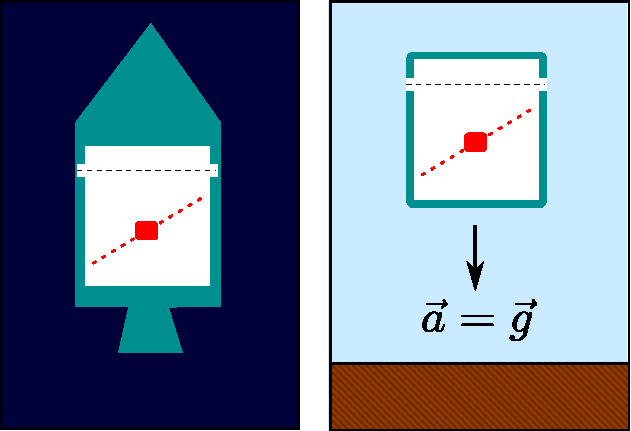
\psfig{file=fig/fig-equivalencia.pdf,height=4cm,angle=0}}
\caption{Equivalencia entre un SRI en ausencia de gravedad y un SR en caida libre.}
\label{fig:equiv2}
\end{figure}
\end{center}

Este resultado establece cierta relaci'on de \textit{equivalencia} en lo que respecta a la mec'anica (es decir, al movimiento de cuerpos) en campos gravitacionales \textit{estacionarios y homog'eneos} y en \textit{SR's acelerados}. Por ejemplo, en un sistema de referencia \textit{en ca'ida libre}, es decir, con $\vec{a}=\vec{g}$, tendremos que cada part'icula describir'a una trayectoria rectil'inea con velocidad constante respecto a $K'$, \textit{tal como lo har'ia en un SRI en el que no existiese campo gravitacional}. Ver figura \ref{fig:equiv1}.
En otras palabras, parece posible ``eliminar'' los efectos de un campo gravitacional (estacionario y homog'eneo) sobre el movimiento de cuerpos, refiriendo estos movimientos a un SR en ca'ida libre\footnote{Ver, por ejemplo, el siguiente \href{http://youtu.be/1ieR8hIXUIg}{video} y tambi'en \href{http://youtu.be/xsNFqMtNZvI}{\'este}.}.
An'alogamente, si consideramos una regi'on muy lejos de todo cuerpo masivo que genere un campo gravitacional ($\vec{g}=\vec{0}$), entonces es posible ``simular'' (los efectos mec'anicos de) un campo gravitacional (estacionario y homog'eneo) describiendo los movimientos desde un SR acelerado (por ejemplo, con aceleraci'on $\vec{a}=-\vec{g}$). Ver figura\footnote{Adaptada a partir de  \href{http://commons.wikimedia.org/wiki/File:Elevator_gravity.svg}{esta} figura original.} \ref{fig:gya}.
\begin{figure}[H]
 \begin{center}
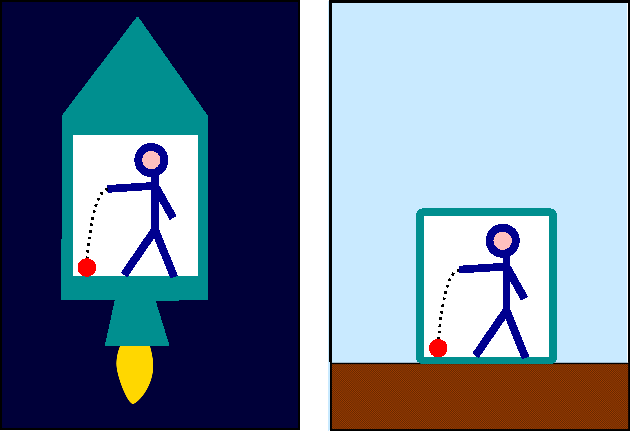
\includegraphics[height=4cm]{fig/fig-gravedad-y-aceleracion.pdf}
\caption{Equivalencia entre campo gravitacional y aceleraci'on.}
\label{fig:gya}
\end{center}
\end{figure}
Note que la existencia de esta equivalencia entre efectos gravitacionales y efectos inerciales depende crucialmente del car'acter universal de la interacci'on gravitacional (en otras palabras, de la validez del PED).

\section{Principio de Equivalencia de Einstein y Sistemas de Referencia Localmente inerciales}
Tal como hemos discutido, la experiencia suministra evidencia a favor de que la interacci'on gravitacional posee las siguientes caracter'isticas:
\begin{quotation}
En una regi'on (espacio-temporal) suficientemente peque\~na (donde las inhomogeneidades del campo puedan ser despreciadas), y respecto a un SR \textit{en ca'ida libre}, las trayectorias de \textit{todo} (peque\~no) cuerpo, libre de fuerzas no-gravitacionales, \textit{son l'ineas rectas con velocidad constante}.
\end{quotation}

Note adem'as que suficientemente lejos de otras distribuciones de masa, donde el campo gravitacional pueda considerarse como nulo, los SR's en ca'ida libre son los usuales SRI's. En este sentido, al menos en lo que respecta a la trayectoria de cuerpos no sometidos a fuerzas no-gravitacionales, los SR's en ca'ida libre juegan el mismo rol f'isico que los SRI's en ausencia de gravedad. Einstein supuso que estos SR's en ca'ida libre son \textit{en toda situaci'on}, es decir\marginnote{Principio de Equivalencia de Einstein}, \textit{para todo tipo de fen'omeno f'isico} (no s'olo mec'anico, tambi'en por ejemplo, electromagn'etico), equivalentes a los SRI's en ausencia de gravitaci'on. Por esta raz'on, y dada la extensi'on finita de estos SR's en ca'ida libre, 'estos son tambi'en llamados \textbf{Sistemas de Referencia Localmente Inerciales} (SRLI's). Este supuesto es tambi'en llamado \textbf{Principio de Equivalencia Fuerte} (PEF), en contraste al PED, que se refiere s'olo a la \emph{mec'anica} de los cuerpos (macrosc'opicos).

La primera referencia conocida al PEF se encuentra en el art'iculo de 1907 de Einstein \cite{Einstein07}, cuyo t'itulo podr'ia traducirse ``Sobre el Principio de Relatividad y las consecuencias que de 'el se desprenden".
 Casi al final de este trabajo (p'agina 454) Einstein escribe 
\begin{quotation}
``Wir... wollen ... in folgenden die v\"ollige physikalische Gleichwertigkeit von Gravitationsfeld und entsprechender Beschleunigung des Bezugssystems annehmen",
\end{quotation}
que se traducir'ia como ``queremos suponer la completa equivalencia f'isica de un campo gravitacional y la correspondiente aceleraci'on del sistema de referencia". Acto seguido (en el resto del paper) Einstein estudia las primeras consecuencias de esta suposici'on.
 
El PEF obliga a repensar la existencia y el rol de los Sistemas de Referencia Inerciales. En la mec'anica de Newton y en RE los SRI's juegan un papel fundamental. Un SRI es entendido como un sistema de ejes rectos ortogonales respecto a los cuales un cuerpo libre de fuerzas externas se mueve en l'inea recta con velocidad constante. Esta abstracci'on resulta entonces ser consistente y 'util s'olo en ausencia de interacci'on gravitacional. En presencia de gravitaci'on, por otro lado, \textit{no existen SRI's con extensi'on infinita}. Esto es debido a que, por un lado, de acuerdo al PED, \textit{todas} las trayectorias de cuerpos son afectadas por la gravedad, es decir, no existen cuerpos libres de esta interacci'on. Adem'as, en presencia de campos gravitacionales (no homog'eneos) no existe ning'un SR (``r'igido'' y de extensi'on infinita) respecto al cual los cuerpos se muevan en forma rectil'inea y uniforme.
Sin embargo, en presencia de gravitaci'on los SRLI's s'i tienen realidad f'isica, pero necesariamente tienen una extensi'on finita en el espaciotiempo.
Como los fen'omenos f'isicos no-gravitacionales conocidos son descritos exitosamente en el marco de la Teor'ia Especial de la Relatividad, Einstein supuso en su teor'ia de Relatividad General, que incorpora la gravitaci'on, que \textit{es en los SRLI's en ca'ida libre donde son v'alidas las leyes conocidas en la teor'ia de RE}.

En resumen, en presencia de un campo gravitacional general no existen SRI's \emph{globales} (de extensi'on infinita). No obstante, de acuerdo al PEF s'i es posible encontrar SR's en regiones peque\~nas (los SRLI's, es decir, SR's en ``caida libre'') donde las leyes de RE son v'alidas. Un campo gravitacional no nulo est'a entonces caracterizado por el hecho que los SRLI's no pueden ``unirse'' para formar un SRI global. Adem'as, si bien en un SRLI no es posible detectar efectos de la gravedad, s'i es posible hacerlo comparando cantidades f'isicas en \textit{distintos} SRLI's. Por ejemplo, en presencia de campo gravitacional no nulo los SRLI's \textit{aceleran entre s'i}, ver figura \ref{fig:SRLI}.
\begin{figure}[H]
\centering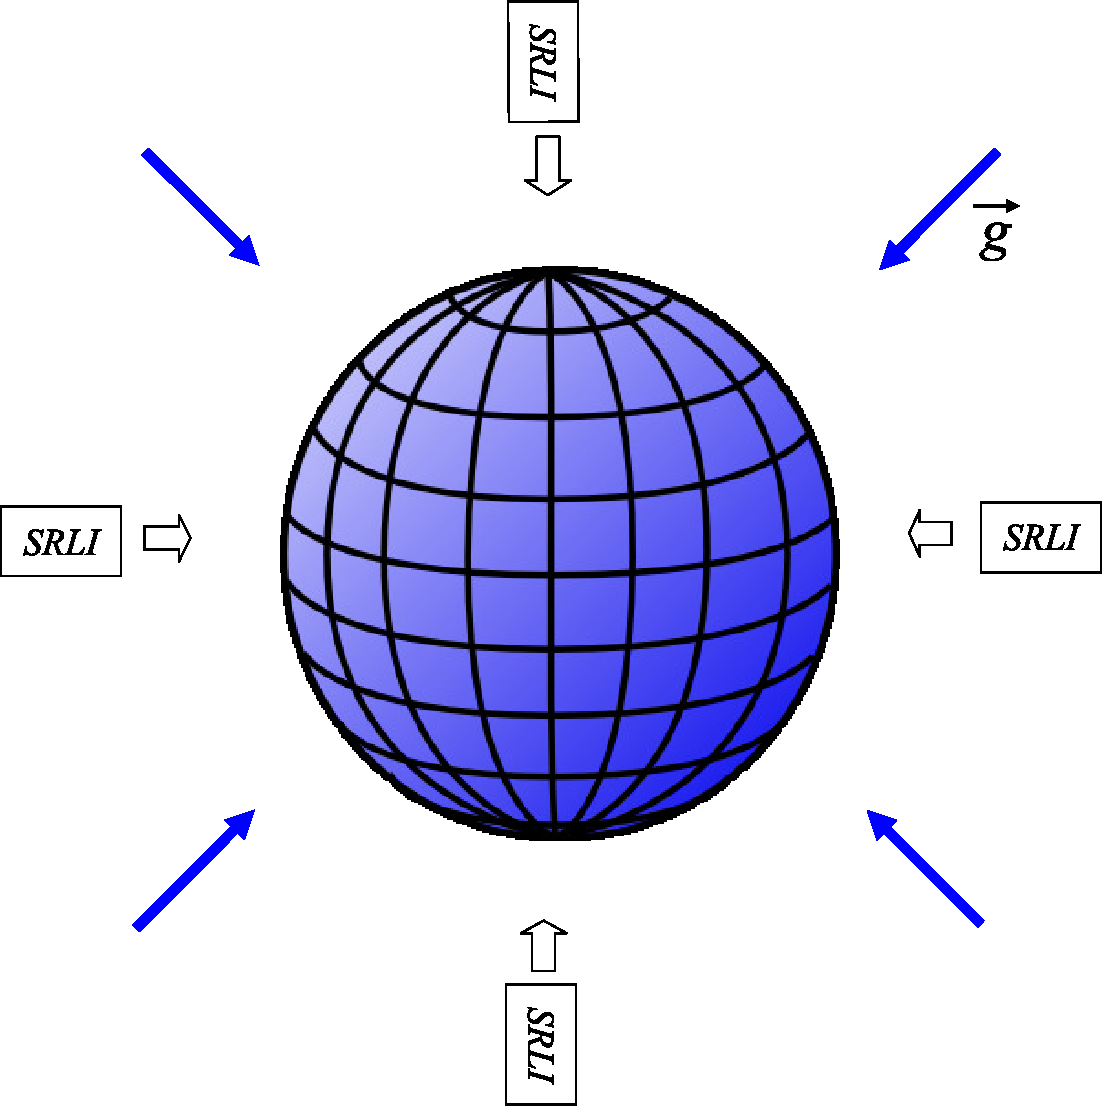
\epsfig{file=fig/fig-SRLI.pdf, width=6cm}
\caption{Sistemas de referencia localmente inerciales cayendo hacia la Tierra.}
\label{fig:SRLI}
\end{figure}

Una consecuencia directa del PEF es que \textit{la luz debiese ser deflectada por campos gravitacionales}. En efecto, la hip'otesis planteada por el PEF es que en los SRLI's, es decir, SR en caida libre, son v'alidas las leyes F'isicas conocidas en la teor'ia de RE. En particular las ecuaciones de Maxwell en su forma usual, y sus conocidas implicancias respecto de la propagaci'on de la radiaci'on electromagn'etica, son v'alidas en estos SRLI's. Como consecuencia, es en estos SRLI's en los que la luz debe(r'ia) moverse en l'inea recta con velocidad constante. 
 Por otro lado, respecto a un SR que acelera respecto a estos SRLI's, por ejemplo, en un SR a una distancia fija de la Tierra, la luz debe(r'ia) curvarse. Ver figura \ref{fig:PEF-luz}.
\begin{figure}[H]
\centering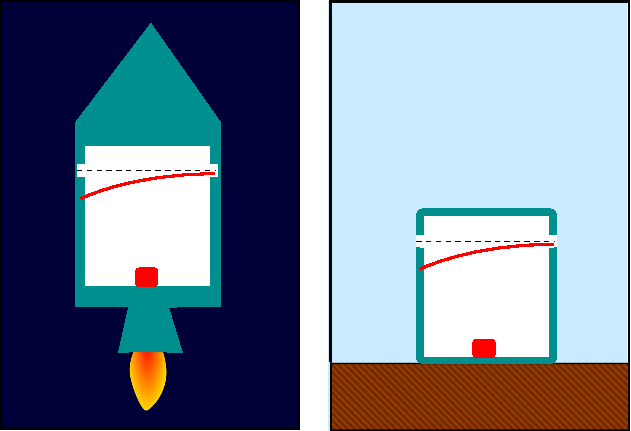
\epsfig{file=fig/fig-gravedad-y-aceleracion-luz.pdf, width=6cm}
\caption{Deflexi'on de la luz. Ambos SR's aceleran respecto a SRLI's.}
\label{fig:PEF-luz}
\end{figure}
Tal como en este caso simple, relacionado con la trayectoria de la luz en un campo gravitacional, el PEF permite determinar c'omo se comporta cualquier sistema f'isico en presencia de un campo gravitacional no nulo (en una regi'on suficientemente peque\~na), ya que es (o debe ser, de acuerdo a este principio) exactamente lo mismo que ocurre cuando el sistema se describe desde un SR que acelera respecto a uno (localmente) inercial. De hecho, el PEF \textit{unifica} localmente (los efectos de) la gravitaci'on con (los de) la aceleraci'on respecto a SRLI's, puesto que son f'isicamente indistinguibles. En este sentido en la teor'ia de gravitaci'on de Einstein la gravedad ``es'' aceleraci'on respecto a SLRI's: el hecho que en una regi'on del espacio se experimente un campo gravitacional respecto a un SR es simplemente una consecuencia de que ese SR acelera respecto a los SRLI's que cubren esa regi'on. Note que estas consideraciones son puramente ``cinem'aticas'' en el sentido que no permiten por si solas determinar la distribuci'on, orientaci'on y din'amica de los SRLI's (exactamente c'omo y hacia donde ``caen'' cada uno de estos SRLI's), 'este es precisamente el rol de las \textbf{ecuaciones de campo de la teor'ia}, que discutiremos en el cap'itulo \ref{capTEG}. No obstante, el PEF determina la forma en que un sistema f'isico responde a un campo gravitacional dado, tal como discutiremos a continuaci'on, ahora en el contexto relativista.

\subsection{Desv'io de la luz*}
\begin{equation}
\Delta t'=\frac{L}{c}, \qquad \Delta y' = 0
\end{equation}
\begin{equation}
\Delta y = \frac{1}{2} g (\Delta t)^2 = \frac{1}{2} g (\Delta t')^2 = \frac{gL^2}{2c^2}
\end{equation}
Si $L\approx 1{\,\rm km} = 10^3{\,\rm m}$, y usando $g\approx 9.8{\,\rm m/s^2}$ entonces
\begin{equation}
\Delta y \approx 5.4\times 10^{-11}{\,\rm m}
\end{equation}
\begin{equation}
\theta \approx \frac{\Delta y}{L} \approx \frac{gL}{2c^2} \approx 5.4\times 10^{-14}
\end{equation}

\subsection{Redshift gravitacional*}
 
 \begin{equation}
 y_{\rm f}(t) = ct, \qquad y_{\rm d}(t)=h+\frac{1}{2}gt^2.
 \end{equation}
 \begin{equation}
t_{\rm d} = \frac{c-\sqrt{c^2-2gh}}{g}
 \end{equation}
 \begin{equation}
 v_{\rm d}=gt_{\rm d} = c-\sqrt{c^2-2gh}
 \end{equation}
 \begin{equation}
 z=\frac{v}{c}=1-\sqrt{1-\frac{2gh}{c^2}} \approx 1-\left(1-\frac{gh}{c^2}\right) = \frac{gh}{c^2} = \frac{\Delta\phi}{c^2}
 \end{equation}
 \begin{equation}
z = \frac{\lambda_{d}-\lambda_{\rm e}}{\lambda_{\rm e}} = \frac{\nu_{\rm e}}{\nu_{\rm d}}-1
 \end{equation}
 \begin{equation}
 \nu_{\rm e}-\nu_{\rm d} \approx \nu_{\rm d}\frac{\Delta\phi}{c^2}
 \end{equation}
  \begin{equation}
 E_{\rm e}-E_{\rm d} \approx E_{\rm d}\frac{\Delta\phi}{c^2}
 \end{equation}
   \begin{equation}
 E_{\rm e} \approx E_{\rm d} + \left(\frac{E_{\rm d}}{c^2}\right)\Delta\phi
 \end{equation}
\section{Observadores acelerados y gravedad: Versi'on  relativista}

Tal como Einstein \cite{Einstein56}, seguiremos considerando que un sistema coordenado (SC) est'a asociado a un SR de modo que un \textit{cambio} de SR queda descrito por una cierta \textit{transformaci'on de  coordenadas} (m'as adelante, sin embargo, veremos que es posible separar estos conceptos: un sistema de coordenadas no necesita siempre estar asociado a un sistema de referencia).

En RE la ecuaci'on que describe el movimiento de una part{\'\i}cula
en ausencia de fuerzas externas, respecto a un SRI $K$, es
\begin{equation}
\frac{d^2x^\mu}{d\tau ^2}=0, \label{tsri}
\end{equation}
donde $x^\mu(\tau )$ es la trayectoria de la part{\'\i}cula,
expresada en coordenadas (pseudo-)cartesianas $x^\mu=(ct,\vec{x})$, y donde $\tau $ es el correspondiente tiempo propio.

De acuerdo a lo discutido en las secciones anteriores, el PEF implica que (\ref{tsri}) ser'a tambi'en la ecuaci'on de movimiento de un cuerpo bajo la acci'on de la gravedad (pero libre de otras fuerzas) \textit{respecto a SRLI's}.

Deseamos ahora transformar la ecuaci'on (\ref{tsri}) para expresarla en t'erminos de las coordenadas asociadas a un SR que no sea un SRLI, es decir, un SR que \textit{acelera} respecto a los SRLI's. La transformaci'on de coordenadas correspondiente debe necesariamente ser \textit{no-lineal} (y mezclar coordenadas espaciales y temporales) para poder describir un cambio a un SR con \textit{aceleraci'on} relativa (las transformaciones de Lorentz, que describen cambios entre SR's con velocidad relativa constante, son lineales). Consideraremos entonces una \textbf{transformaci'on general de coordenadas} (TGC) $x^\mu\rightarrow \bar{x}^\mu(x)$ que en el caso considerado aqu'i describe un cambio desde el (SC asociado al) SRLI $K$ hasta (el SC asociado a) un SR $\bar{K}$ que en general no ser'a localmente inercial\footnote{El nuevo SR ser'a tambi'en localmente inercial si la transformaci'on es una transformaci'on de Lorentz. Adem'as, una TGC no s'olo puede aplicarse para describir transformaciones a SR's con movimiento relativo, sino que tambi'en al caso en que se usan \textit{coordenadas curvil'ineas en un mismo sistema de referencia}. Por ejemplo, la transformaci'on de coordenadas
$x^\mu\to\bar{x}^\mu$ con $x^\mu=(ct,x,y,z)$ y $\bar{x}^\mu=(ct,r,\theta,\varphi)$, donde $(r,\theta,\varphi)$ son las usuales coordenadas esf'ericas se interpreta
como un simple cambio de coordenadas espaciales, \textit{en el mismo SR}. En general, la TC estar'a ligada a un cambio de SR si mezcla coordenadas temporales y espaciales. Ver por ejemplo (\ref{tgan}).}. Respecto al SC $\bar{x}^\mu$ la ecuaci'on de movimiento (\ref{tsri}) adopta la forma
\begin{equation}
\boxed{\frac{d^2\bar{x}^\mu}{d\tau ^2}+\bar{\Gamma }_{\ \nu
\lambda }^\mu\frac{d\bar{x}^{\nu }}{d\tau }\frac{d\bar{x}%
^\lambda }{d\tau }=0.} \label{tsrni}\marginnote{Ec. de mov. en coord. arbitrarias}
\end{equation}
En efecto,
\begin{eqnarray}
\frac{d^2\bar{x}^\mu}{d\tau ^2} &=&\frac{d}{d\tau }\left(
\frac{d\bar{x}^\mu}{d\tau } \right) \\
&=&\frac{d}{d\tau }\left( \frac{\partial \bar{x}^\mu}{\partial x^{\nu
}}\frac{dx^{\nu }}{d\tau }\right) \\
&=&\frac{\partial \bar{x}^\mu}{\partial x^\nu } \frac{d^2x^{\nu }}{d\tau
^2}+\frac{\partial ^2\bar{x}^\mu }{\partial x^{\nu }\partial x^\lambda
}\frac{dx^\lambda }{d\tau }\frac{dx^{\nu }}{d\tau } \\
&=&\frac{\partial ^2\bar{x}^\mu }{\partial x^{\nu }\partial x^\lambda
}\frac{dx^\lambda }{d\tau }\frac{dx^{\nu }}{d\tau } \\
&=&-\bar{\Gamma }_{\ \nu
\lambda }^\mu\frac{d\bar{x}^{\nu }}{d\tau }\frac{d\bar{x}%
^\lambda }{d\tau } ,
\end{eqnarray}
donde definimos
\begin{equation}
\boxed{\bar{\Gamma }_{\ \nu\lambda }^\mu(\bar{x}):=-\frac{\partial
^2\bar{x}^\mu }{\partial x^\alpha \partial x^\beta }\frac{\partial
x^\alpha }{\partial \bar{x}^{\nu }}\frac{\partial x^\beta }{\partial
\bar{x}^\lambda }=\frac{\partial\bar{x}^\mu}{\partial x^\sigma
}\frac{\partial ^2x^\sigma }{\partial \bar{x}^{\nu }\partial \bar{x}^\lambda }.}
\label{defGammaSR}
\end{equation}
As{\'\i}, la ecuaci'on del movimiento de una part{\'\i}cula libre en un SC
general posee, adicionalmente al usual t'ermino proporcional a la
segunda derivada de la 4-posici'on, un t'ermino \textit{bilineal} en la 4-velocidad. Este segundo t'ermino describe las llamadas ``fuerzas inerciales''\footnote{'Este es el t'ermino que, en los l'imites apropiados, reproduce la aceleraci'on de Coriolis en un SR rotante, o el segundo t'ermino del lado derecho de (\ref{acelprima}).}.

Simult'aneamente, el elemento de l'inea (el tiempo propio, para el caso de separaciones tipo tiempo), adopta la forma
\begin{equation}\marginnote{Elemento de l'inea en coord. arbitrarias}
 \boxed{ds^2=\bar{g}_{\mu\nu }(\bar{x})\,d\bar{x}^\mu d\bar{x}^{\nu },}
\end{equation}
con
\begin{equation}\marginnote{m'etrica en coord. arbitrarias}
\boxed{\bar{g}_{\mu\nu }(\bar{x}):=\eta _{\lambda \rho }\,\frac{\partial x^\lambda }{\partial \bar{x}^\mu}\frac{\partial x^\rho }{\partial \bar{x}^{\nu }}.} \label{tm}
\end{equation}
Recuerde que tanto en \eqref{defGammaSR} como en \eqref{tm} las coordenadas $x^\mu$ est'an asociadas a un SRLI.

Derivando (\ref{tm}) y usando (\ref{defGammaSR}) es posible expresar las
componentes de $\bar{\Gamma }$ directamente en t'erminos de las (derivadas de las)
componentes de $\bar{g}$:
\begin{equation}
\boxed{\bar{\Gamma }_{\ \nu\lambda }^\mu\equiv \frac{1}2\bar{g}^{\mu\rho}\left(
\bar{\partial}_\nu\bar{g}_{\lambda\rho}+\bar{\partial}_\lambda\bar{g}_{\nu\rho}
-\bar{\partial}_\rho\bar{g}_{\nu\lambda}\right) ,}
\end{equation}
donde $\bar{g}^{\mu\rho}(\bar{x})$ son las componentes de la \textbf{inversa} de
$\bar{g}_{\mu\nu}(\bar{x})$, definida de modo que (en cada evento)
\begin{equation}
\bar{g}^{\mu\rho}(\bar{x})\,\bar{g}_{\rho\nu}(\bar{x})=\delta^\mu_\nu.
\end{equation}


Vemos con esto que, en peque\~nas regiones del espaciotiempo, pero respecto a SR's generales (asociados a coordenadas $\bar{x}$), los efectos del campo gravitacional sobre la trayectoria de cuerpos quedan descritos por las cantidades $\bar{\Gamma }_{\ \nu\lambda }^\mu$ (con 40 componentes linealmente independientes!) que miden ``que tan no-(localmente-)inercial'' es el SR. \textit{Simult'aneamente}, los coeficientes $\bar{g}_{\mu\nu}(\bar{x})$ que determinan el elemento de l'inea, y por consiguiente el tiempo propio, \textit{dejan de ser constantes y diagonales}  (10 componentes linealmente independientes!).

Para estudiar c'omo cambian estas cantidades entre SC's arbitrarios (es decir, ninguno de ellos asociados, en general, a SRLI's), efectuamos una segunda TGC $\bar{x}^\mu\rightarrow
\tilde{x}^\mu(\bar{x})$. Como es de esperar, se encuentra que la ecuaci'on de movimiento de la part{\'\i}cula (libre de fuerzas no-gravitacionales), expresada en coordenadas $\tilde{x}^\mu$ es nuevamente de la forma (\ref{tsrni}), es decir,
\begin{equation}
\frac{d^2\tilde{x}^\mu}{d\tau ^2}+\tilde{\Gamma }_{\ \nu
\lambda }^\mu\frac{d\tilde{x}^{\nu }}{d\tau }\frac{d\tilde{x}%
^\lambda }{d\tau }=0, \label{tsrni2}
\end{equation}
donde
\begin{eqnarray}
\tilde{\Gamma }_{\ \nu\lambda }^\mu(\tilde{x})&:=&
\frac{\partial \tilde{x}^\mu}{\partial x^\sigma }\frac{\partial
^2x^\sigma }{%
\partial \tilde{x}^{\nu }\partial \tilde{x}^\lambda } \\
&=&\frac{\partial
\tilde{x}^\mu}{\partial \bar{x}^\sigma }\frac{\partial
\bar{x}^\rho }{\partial \tilde{x}^{\nu }}\frac{\partial
\bar{x}^{\eta }}{\partial \tilde{x}^\lambda }\bar{\Gamma }_{\ \rho \eta
}^\sigma (\bar{x})+\frac{\partial \tilde{x}^\mu}{%
\partial \bar{x}^\rho }\frac{\partial ^2\bar{x}^\rho }{%
\partial \tilde{x}^{\nu }\partial \tilde{x}^\lambda }. \label{tigam} \marginnote{ley de transf. de conexi'on}
\end{eqnarray}

Vemos que los coeficientes $\Gamma$ transforman \textit{inhomog'eneamente} bajo
una TGC. Esta propiedad es precisamente la que posibilita que $\Gamma$ sea nulo
en coordenadas pseudo-cartesianas asociadas a SRLI's, pero distinto de cero en coordenadas asociadas a SR's que aceleran respecto a los primeros. M'as precisamente, los coeficientes $\Gamma$ \emph{transforman como una conexi'on} bajo una TGC.

Por otro lado, las componentes de la m'etrica en el SR $\tilde{K}$, con coordenadas $\tilde{x}$, est'an relacionadas con las componentes en $\bar{K}$ por medio de
\begin{equation}
 \tilde{g}_{\mu\nu}(\tilde{x})=\frac{\partial\bar{x}^\lambda}{\partial \tilde{x}^\mu}
\frac{\partial\bar{x}^\rho}{\partial \tilde{x}^\nu}\,\bar{g}_{\lambda\rho}(\bar{x}).  \marginnote{ley de transf. de m'etrica}
\end{equation}

M'etricas no constantes, conexiones no nulas (as'i como curvaturas y torsiones, etc.) son objetos matem'aticos definidos usualmente en el contexto de la \textit{geometr'ia diferencial} y en particular de la \textit{geometr'ia riemanniana}, o geometr'ia de \textit{espacios curvos}. En el cap'itulo \ref{cap:tensores} resumiremos algunos aspectos b'asicos de este vasto tema.

%\section{Relatividad especial y gravitaci'on newtoniana: un conflicto}
%
%En la teor'ia de la Relatividad Especial, los eventos ocurren en el
%espaciotiempo 4-dimen\-sio\-nal. Existen adem'as observadores
%``privilegiados'', los observadores inerciales. Ellos son entendidos como marcos
%infinitamente extendidos en espacio y tiempo en los que cuerpos \textit{libres}
%(que no son influenciados por ning'un otro cuerpo) se mueven con velocidad
%constante en l'ineas rectas en
%el sentido geom'etrico euclidiano. A estos SRI's asociamos un conjunto de
%coordenadas \textit{inerciales}, tambi'en llamadas (pseudo-)cartesianas,
%$x^\mu=(x^0,x^1,x^2,x^3)$. En el espacio vac'io y respecto a un SRI no existe
%preferencia entre los distintos puntos e instantes y adem'as no existe una
%direcci'on preferente. Decimos que el vac'io es invariante bajo translaciones
%(espaciales y temporales) y bajo rotaciones. Adem'as, el principio de
%relatividad establece que todos los SRI's, con velocidades relativas constantes
%entre ellos, son f'isicamente equivalentes, es decir, indistinguibles.
%Equivalentemente, las leyes f'isicas son las mismas en todos los SRI's. Esto, a
%fin de cuentas, es tambi'en una \textit{observaci'on}, es decir, una generalizaci'on de resultados experimentales. En RE estas equivalencias entre SRI's se expresan por medio de la covariancia de las ecuaciones respecto a transformaciones de Lorentz y translaciones (es decir, bajo transformaciones de Poincar\`e).
%
%Una teor'ia de la interacci'on gravitacional que sea compatible con los
%principios de la TRE (por ejemplo, con una velocidad m'axima de propagaci'on de
%las interacciones) requiere entonces que sus ecuaciones sean covariantes bajo
%TL's, es decir, que puedan ser escritas en t'erminos de vectores y tensores
%respecto a TL's.
%
%\subsection{Teor'ia escalar de la gravitaci'on*}
%La ecuaci'on newtoniana que determina el campo gravitacional es la ecuaci'on de
%Poisson (\ref{Poisson}). Una posible generalizaci'on covariante bajo TL's
%(an'aloga a la ecuaci'on que satisface el potencial electromagn'etico) es la
%ecuaci'on de onda
%\begin{equation}
%\square\phi=-4\pi G\rho, \label{casicasi}
%\end{equation}
%con $\square=\eta^{\mu\nu}\partial_\mu\partial_\nu$. En este caso la ecuaci'on
%de Poisson para el potencial $\phi$ se encuentra en el caso l'imite de campos
%est'aticos.
%
%Un primer candidato a una teor'ia relativista de la gravitaci'on podr'ia
%considerar que el campo gravitacional $\phi$ es determinado por la ecuaci'on
%(\ref{casicasi}) en el caso general en que tanto $\phi$ como $\rho$ sean
%dependientes del tiempo. Pero, ?`cu'al es el significado de la fuente $\rho$ en
%este caso?. En el caso de un fluido sin presi'on (polvo), o un conjunto de
%part'iculas puntuales donde todas las componentes se mueven con la misma
%velocidad, es posible construir un escalar proporcional a la densidad de masa
%(la densidad de masas en reposo $\rho$ vista anteriormente). Por otro
%lado, en RE la masa no es entendida como una cantidad independiente, sino
%s'olo como una componente de la energ'ia de los cuerpos. As'i,
%en una teor'ia relativista de la gravitaci'on esperamos que todo el contenido de
%energ'ia de un cuerpo aporte su a masa gravitacional. Esto significa que podemos
%intentar reemplazar densidad de masa por densidad de energ'ia como fuente del
%campo gravitacional. De este modo, para completar nuestra generalizaci'on
%(\ref{casicasi}) necesitamos una cantidad escalar bajo TL's que contenga la
%densidad de energ'ia y que se reduzca a la usual densidad de masa en los casos
%l'imites apropiados.
%
%A partir del tensor de energ'ia-mom'entum $T^{\mu\nu}$ de una distribuci'on de
%materia podemos construir el siguiente escalar:
%\begin{equation}
%T:=T^\mu_{\ \mu}=\eta_{\mu\nu}T^{\mu\nu}.
%\end{equation}
%En el caso de un fluido ideal,
%\begin{equation}
%T=\left( \rho +\frac{p}{c^2}\right) u^\mu u_\mu-p\delta^\mu_\mu=\left( \rho
%+\frac{p}{c^2}\right) c^2-4p=\rho c^2-3p.
%\end{equation}
%Para ``materia no-relativista'', $p\ll \frac{1}{3}\rho c^2$ (verificar esta
%condici'on para un gas ideal) tenemos $T=\rho c^2$, de modo que podemos
%postular
%\begin{equation}
%\square\phi=-\kappa T, \label{casicasi2}
%\end{equation}
%con $\kappa:=\frac{4\pi G}{c^2}$.
%A primera vista, lo anterior define una teor'ia relativista viable de la
%gravitaci'on. De hecho, la teor'ia es \textit{matem'aticamente consistente}. Sin
%embargo, se encontr'o que esta \textit{teor'ia escalar de la gravitaci'on no
%describe adecuadamente las observaciones}. En general, una teor'ia gravitacional
%escalar no permite describir el fen'omeno de deflecci'on de la luz por campos
%gravitacionales, debido a que un campo escalar no puede acoplarse razonablemente
%al campo electromagn'etico (ya que el tensor de enrg'ia-mom'entum
%electromagn'etico tiene traza nula). Por otro lado, hoy en d'ia la desviaci'on
%de la luz por campos gravitacionales es un hecho experimental confirmado m'as
%all'a de toda duda. En resumen, debemos considerar otras posibilidades para una
%teor'ia relativista de la gravitaci'on.
%


\chapter{An'alisis tensorial y geometr'ia diferencial}\label{cap:tensores}

\section{Variedades diferenciables}

\textbf{Definici'on:} Una variedad diferenciable $n$-dimensional $M$ es
un conjunto continuo de puntos que puede ser cubierto completamente por un
conjunto contable de vecindades abiertas $U_1, U_2,\dots$ sobre los cuales pueden ser definidos sistemas coordenados ($n$-dimensionales) cont'inuos y diferenciables, tales que en las intersecciones de dichas vecindades, sus correspondientes sistemas est'an relacionados unos a otros por transformaciones de coordenadas diferenciables.

Una variedad puede ser concebida b'asicamente como un espacio de
dimensi'on $n$, an'alogo a una superficie $n$-dimensional. En general,
es posible que ella no pueda ser cubierta completamente por un 'unico sistema coordenado.
Curvas y superficies en el espacio $n$-dimensional $R_n$ son ejemplos de variedades.
\begin{center}
\begin{figure}[H]
\centerline{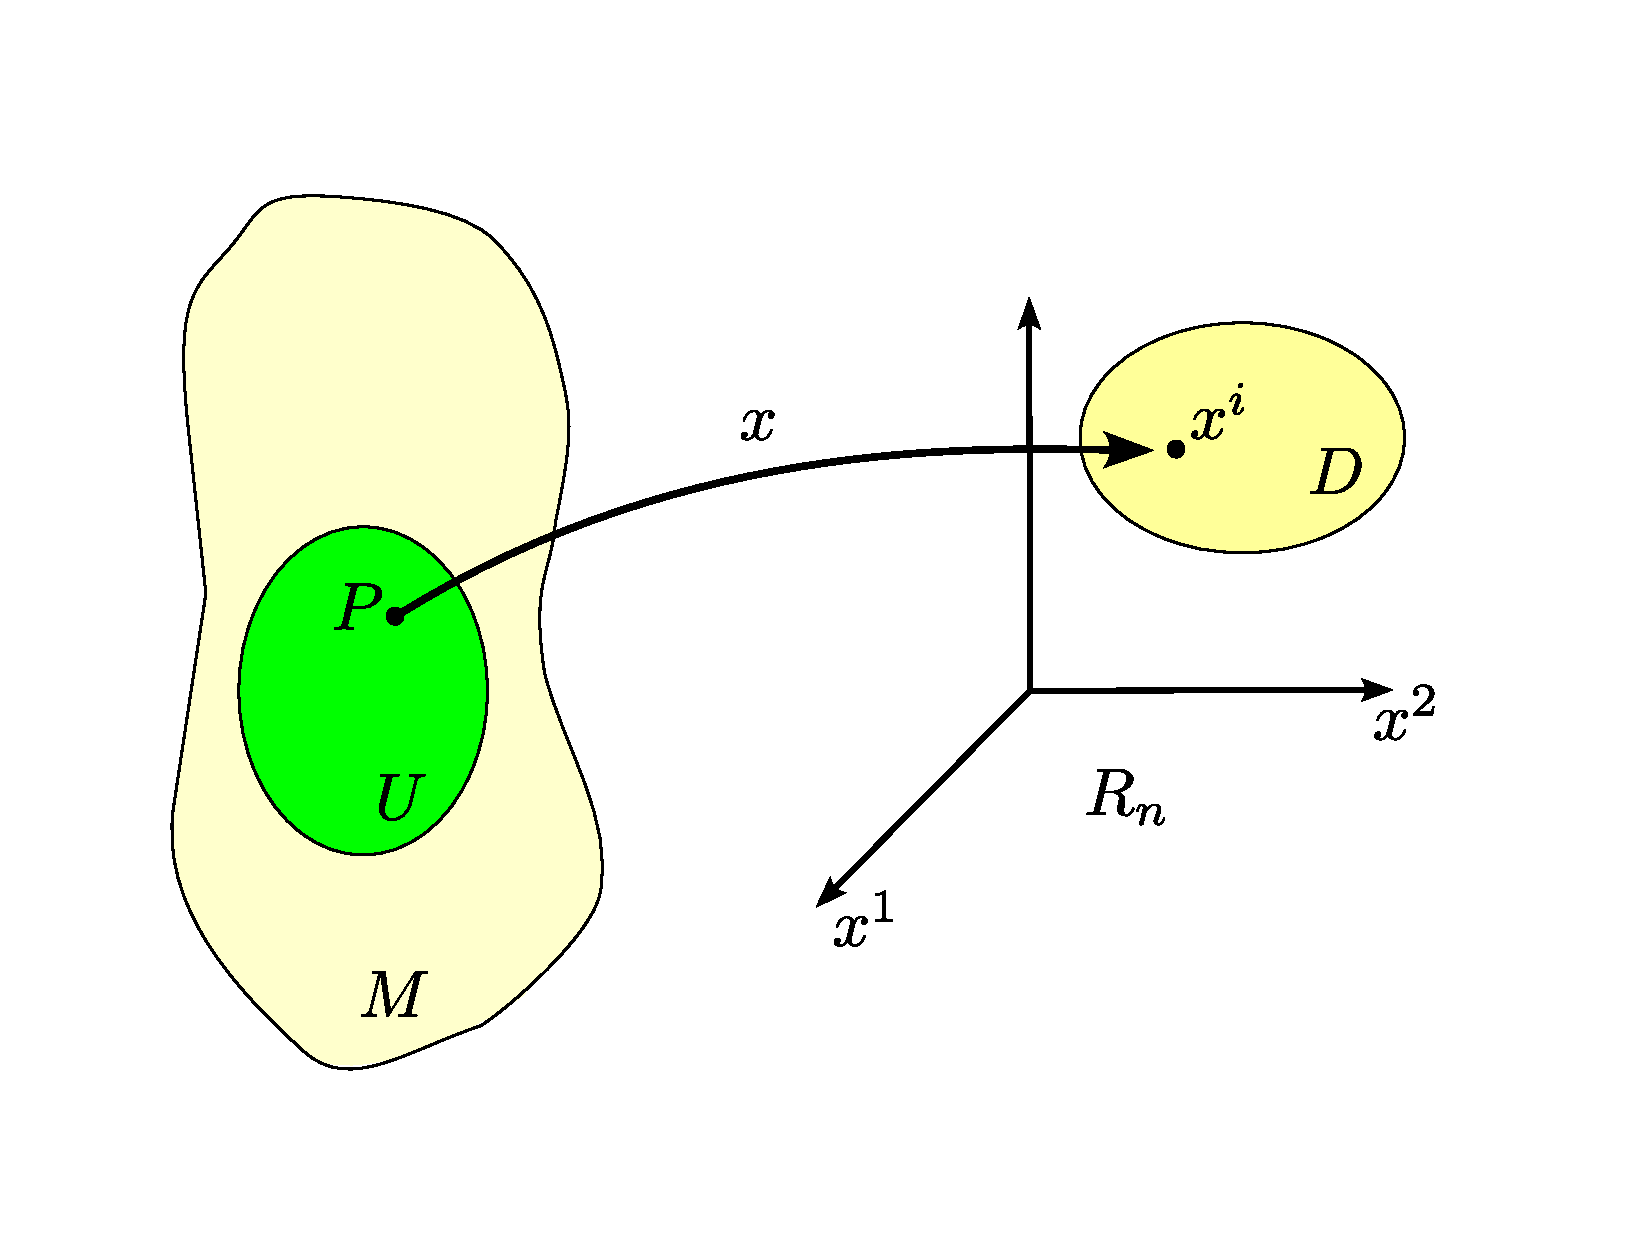
\psfig{file=fig/fig-coordenadas.pdf,height=6cm,angle=0}}
\caption{Una variedad y un sistema coordenado.}
\label{1-1}
\end{figure}
\end{center}

Como vemos en la figura \ref{1-1}, sobre cada vecindad $U$ pueden definirse sistemas coordenados (SC's) que asignan un'ivocamente a cada punto $P\in U$
un conjunto ordenado de n'umeros $x^i=(x^1,\dots ,x^n)$,
$i,j,\dots =1,\dots ,n$, llamados \textit{coordenadas de} $P$. Se exige que este mapeo uno a
uno sea continuo, de modo que, cuando $P$ se mueve en $U$, la correspondiente $n$-upla
($x^1,\dots ,x^n$) se mueve continuamente en un dominio $D$ contenido en $R_n$. Tambi'en se supone que la dimensi'on $n$ del mapeo de puntos de $M$ a $R_n$ es siempre la misma, en la vecindad de cada punto de la variedad.
\begin{center}
\begin{figure}[H]
\centerline{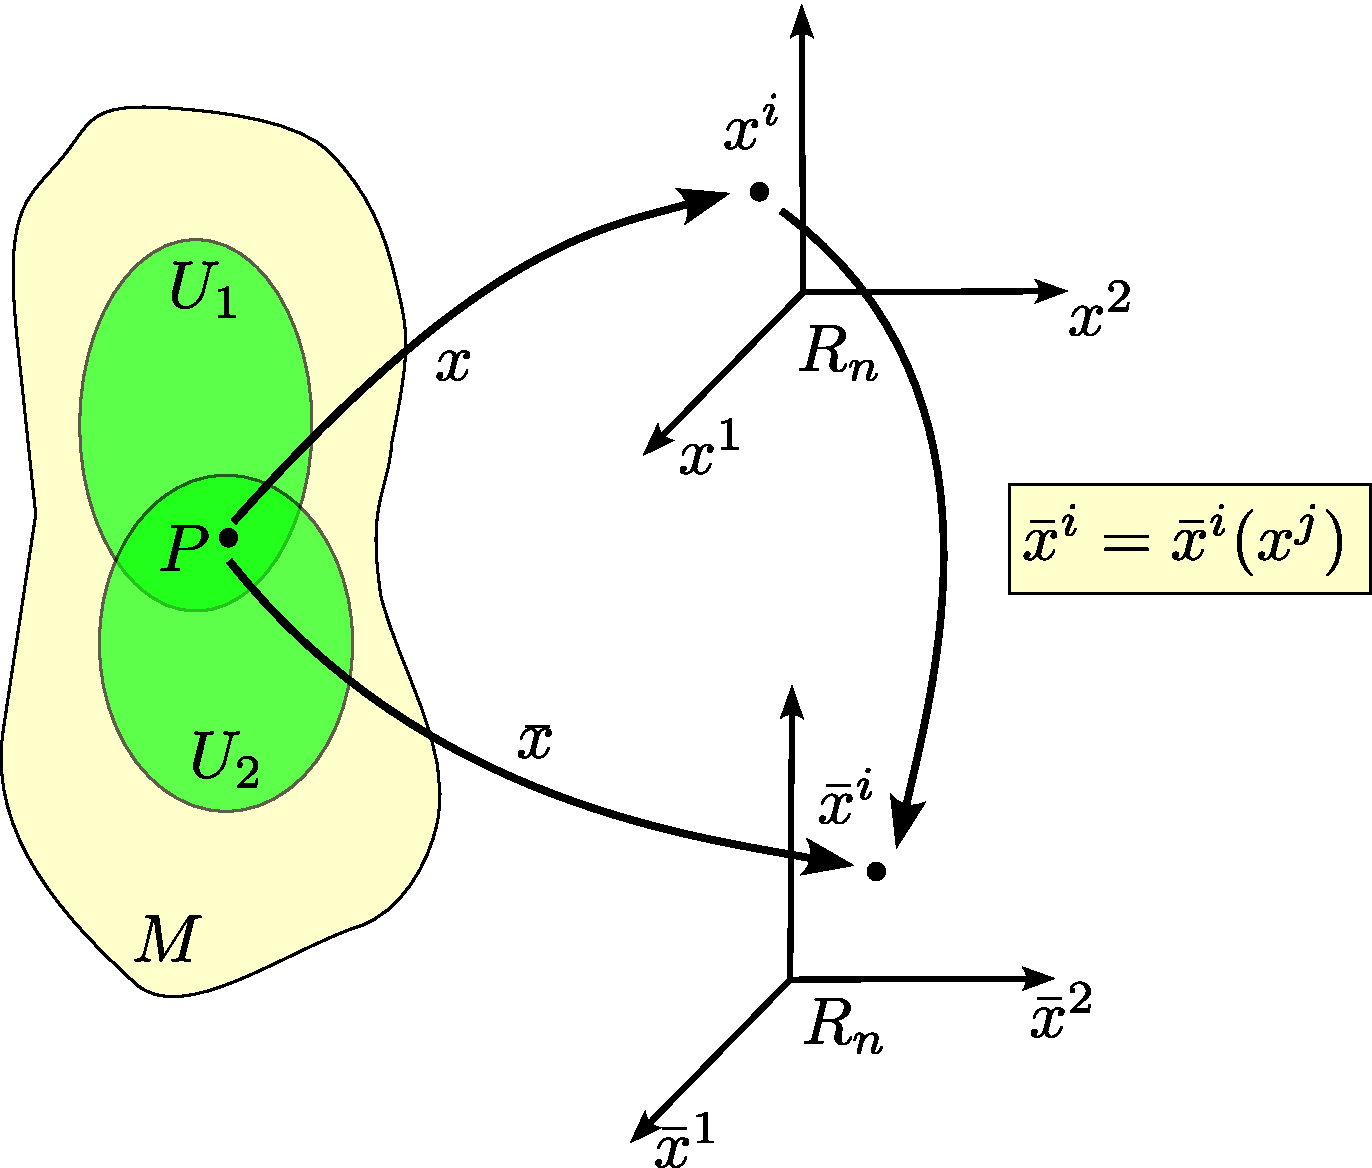
\psfig{file=fig/fig-cambio-coordenadas.pdf,height=6cm,angle=0}}
\caption{Una variedad y dos sistemas coordenados.}
\label{2-1}
\end{figure}
\end{center}

Consideremos la figura \ref{2-1}. El conjunto $M$ es una variedad diferenciable
si para cada punto $P$ en la
intersecci'on de dos abiertos, $U_1$, $U_2$ $\subseteq M$, los
correspondientes sistemas de coordenadas est'an relacionados por transformaciones diferenciables e invertibles: 
\begin{equation}
\bar{x}^j  =\bar{x}^j (x^i ), \qquad x^i  =x^i (\bar{x}^j ),\label{v1}
\end{equation}
de modo que, en cada punto de $U_1\cap U_2$,
\begin{equation}
\frac{\partial x^i }{\partial\bar{x}^j }\frac{\partial\bar{x}^j }{\partial
x^k }=\delta_k ^i, \qquad \frac{\partial\bar{x}^j }{\partial x^i 
}\frac{\partial x^i }{\partial\bar{x}^l }=\delta_l ^j , \label{v2}
\end{equation}
y adem'as
\begin{equation}
\frac{\partial(x^1,\dots ,x^n)}{\partial(\bar{x}^1
,\dots ,\bar{x}^n)}\cdot\frac{\partial(\bar{x}^1,\dots
,\bar{x}^n)}{\partial (x^1,\dots ,x^n)}=1. \label{v3}
\end{equation}

\section{Escalares, vectores y tensores}

En una variedad dada, es posible (y 'util) definir cantidades que representen magnitudes de inter'es f'isico. Estas cantidades pueden en general poseer componentes cuyos valores dependen del sistema de coordenadas usado para describir una cierta regi'on de la variedad. Por esto, es importante estudiar c'omo cambian las distintas cantidades definidas sobre una variedad bajo TGC's, clasific'andolas de acuerdo a la ley de transformaci'on que satisfacen. A continuaci'on estudiaremos la definici'on de vectores y tensores bajo TGC's. Note que los tensores no agotan todas las cantidades 'utiles de definir en una variedad\footnote{Por ejemplo, en algunas aplicaciones es 'util considerar objetos llamados \textbf{densidades tensoriales}, cuya ley de transformaci'on es distinta a los de los tensores. Adem'as, m'as adelante definiremos objetos llamados \textbf{conexiones}, que tampoco son tensores.}

\subsection{Escalares}
El caso m'as simple de una magnitud definida sobre una variedad es aquel en que se asocia un valor (real) a cada punto $P\in M$, el cual, por definici'on, no cambia bajo una transformaci'on de coordenadas (TC) arbitraria.

\begin{quotation}
\textbf{Definici'on:} Una cantidad real $\phi$, definido en un punto $P$ de la variedad $M$, es un \textbf{escalar} si bajo toda TGC se verifica que
\begin{equation}\marginnote{Escalar}
\boxed{\bar{\phi}(P)=\phi(P).} \label{t1}
\end{equation}
\end{quotation}

\subsection{Vectores contravariantes}

Consideremos dos puntos $P$ y $Q$, infinitesimalmente pr'oximos, de la variedad
$M$. Las respectivas coordenadas de estos puntos en un SC $x$ son
\begin{equation}
x^i(P)=x^i, \qquad x^i(Q)=x^i+dx^i.
\end{equation}
En otro SC $\bar{x}$, relacionado con el original por medio de (\ref{v1}),
tendremos
\begin{equation}
\bar{x}^i(P)=\bar{x}^i, \qquad \bar{x}^i(Q)=\bar{x}^i+d\bar{x}^i. \label{xP}
\end{equation}

Encontremos ahora la relaci'on entre las diferencias coordenadas $d\bar{x}^i$ y $dx^i$.
Usando (\ref{v1}) y (\ref{xP}b) podemos escribir
\begin{equation}
\bar{x}^i(Q)=\bar{x}^i(x(Q))=\bar{x}^i(x^j+dx^j)=\bar{x}^i(x^j)+\frac{
\partial\bar{x}^i}{\partial x^j}(x)dx^j,
\end{equation}
de modo que obtenemos
\begin{equation}\marginnote{Transf. de diferencias coordenadas}
\boxed{d\bar{x}^i_{P\rightarrow Q}=\frac{\partial\bar{x}^i}{\partial
x^j}(P)\,dx^j_{P\rightarrow Q}.} \label{tdx}
\end{equation}

Por tanto, bajo un cambio de SC, las diferencias de coordenadas entre puntos $P$ y
$Q$ infinitesimalmente pr'oximos cambian su valor, pero est'an relacionados por
medio del Jacobiano de la TGC, \textit{evaluado en el punto $P$}. La ley de
transformaci'on (\ref{tdx}) es el modelo para definir lo que llamaremos un
\textbf{vector contravariante}.

\begin{quotation}
\textbf{Definici'on:} Se dice que un conjunto de $n$ n'umeros
$A^i(P)=(A^1,\dots ,A^n)$, definidos en cada SC $x$, son las componentes  de un
\textbf{vector contravariante en un punto} $P$ (en el SC $x$), si bajo cada TGC (\ref{v1}), dichas componentes obedecen la siguiente ley de transformaci'on:
\begin{equation}\marginnote{Vector contravariante}
\boxed{\bar{A}^i(P)=\frac{\partial\bar{x}^i}{\partial x^j}(P)A^j(P).} \label{t9}
\end{equation}
\end{quotation}

De esta forma, la diferencia de coordenadas entre dos puntos infinitesimalmente pr'oximos $P$ y $Q$ define un vector contravariante infinitesimal en $P$. Equivalentemente, si $\cal C$ es una curva en $M$ (e.d. una subvariedad unidimensional de $M$), parametrizada (en una cierta vecindad y en alg'un SC definido en ella) por $x^i=x^i(\lambda)$ donde $\lambda$ es un par'ametro real continuo, entonces los \textbf{vectores tangentes} $A^ i(P):=(dx^i/d\lambda)(\lambda_P)$ son componentes de un vector contravariante asociado al punto $P$ (con coordenadas $x^i(P)=x^i(\lambda_P)$).

Se debe enfatizar que la ley de transformaci'on anterior define un vector
contravariante \textit{asociado a un punto dado} de la variedad. Esta identificaci'on de un vector con un punto de la variedad es necesaria ya que el jacobiano  ${\partial\bar{x}^i}/{\partial x^j}$ \textit{no es constante en general}, es decir, su valor depende del punto donde es evaluado. En general, cada punto de la variedad puede tener asociado infinitos vectores contravariantes. Es
f'acil comprobar que si $A^i(P)$ es un vector contravariante definido en un
punto $P$ dado, entonces $\alpha A^i(P)$ (donde $\alpha$ es un escalar) es un
nuevo vector contravariante en el punto $P$. An'alogamente, dado dos vectores
contravariantes $A^i(P)$ y $B^i(P)$ definidos \textit{en el mismo punto}
entonces $\alpha A^i(P)+\beta B^i(P)$ es tambi'en un vector contravariante en
$P$ (para valores arbitrarios de los escalares $\alpha$ y $\beta$). En otras
palabras, el conjunto de vectores contravariantes definidos \textit{en un mismo punto} $P$ define un \textbf{espacio vectorial $n$-dimensional}, que llamaremos \textbf{espacio tangente en $P$}: $T_n(P)$. \marginnote{Espacio Tangente}

Es importante destacar que los vectores contravariantes definidos en $P$ son
elementos del espacio tangente de $P$, y \textit{no son elementos de} $M$ (los
elementos de $M$ son los \textit{puntos} de la variedad). Note adem'as que las componentes $x^i$ de un punto $P$ de $M$ \textit{no son componentes de un vector} contravariante\marginnote{Coords. no son vectores bajo TGC's}, simplemente porque su ley de transformaci'on bajo TGC's es dada por (\ref{v1}), que es diferente de (\ref{t9})\footnote{Ambas leyes de transformaci'on, de las coordenadas y de vectores contravariantes, coinciden s'olo si restringimos nuestra atenci'on a transformaciones \textit{lineales} de coordenadas, de la forma $\bar{x}^i=L^i_{\ j}x^j$, donde $L^i_{\ j}$ son (en general 16 valores independientes) \textit{constantes}. Este hecho justifica porqu'e en mec'anica newtoniana y en la Teor'ia Especial de la Relatividad s'i es posible considerar las coordenadas como vectores, bajo rotaciones y transformaciones de Lorentz, respectivamente.}

\subsubsection{Representaci'on pict'orica de vectores contravariantes}
Es posible representar pict'oricamente un vector contravariante $A^i(P)$ por
medio de una ``flechita'' (infinitesimal) a partir del punto $P$. M'as detalladamente, dado un
vector contravariante $A^i(P)$ en $P$ es posible asociar consistentemente (esto quiere decir, independiente del SC usado) un punto $Q$ infinitesimalmente pr'oximo a $P$. En un SC dado (pero arbitrario) con coordenadas $x^i$, definimos las componentes del nuevo punto $Q$ por
\begin{equation}
x^i(Q):=x^i(P)+\varepsilon A^i(P), \label{defQ}
\end{equation}
donde $\varepsilon$ es un \textit{par'ametro escalar infinitesimal}.

La ley de transformaci'on de $A^i(P)$, es decir, el hecho 'este que sea un vector contravariante, asegura que la definici'on del punto $Q$ de la variedad por medio de (\ref{defQ}) sea independiente del SC usado. [En realidad, un vector contravariante define s'olo la \textit{direcci'on} de la correspondiente flechita, la ubicaci'on del punto $Q$ depende tambi'en del par'ametro infinitesimal $\varepsilon$].

Equivalentemente, es posible definir la representaci'on pict'orica de vectores contravariantes asoci'andoles una curva $\cal C$ (al menos, en alguna vecindad que incluya al punto $P$) tal que su vector tangente en $P$ sea igual (o proporcional, con una constante de proporcionalidad positiva) al vector $A^i(P)$, es decir, tal que $(dx^i/d\lambda)(P)=A^i(P)$.

\subsection{Vectores covariantes}

Consideremos un campo escalar $\phi$ definido en una regi'on de la variedad. En
un SC $x$ tendremos una dependencia expl'icita $\phi(x)$, y podemos calcular
las derivadas de $\phi$ respecto a las coordenadas $x^i$, es decir, el gradiente
del campo $\phi$, ${\partial \phi}/{\partial x^i}$, que define nuevos
campos. An'alogamente, si usamos un nuevo SC $\bar{x}$, tendremos otras
funciones expl'icitas $\phi(\bar{x})$ y podemos calcular el correspondiente
gradiente ${\partial \phi}/{\partial \bar{x}^i}$. En un punto $P$ dado,
podemos relacionar estos gradientes usando la transformaci'on coordenada
(\ref{v1}) y la regla de la cadena:
\begin{equation}
\boxed{\frac{\partial\phi}{\partial \bar{x}^i }(\bar{x}(P))=\frac{\partial x^j
}{\partial\bar{x}^i }(P)\frac{\partial\phi}{\partial x^j }(x(P)).} \label{tt2}
\end{equation}
Comparando (\ref{tt2}) con (\ref{t9}) vemos que las $n$ cantidades definidas por
\textit{el gradiente de un campo escalar} (calculado respecto a un SC) \textit{no forman
un vector contravariante}. En otras palabras, las derivadas de un campo escalar definen un nuevo tipo de objeto, que llamaremos \textbf{vector covariante}.

\begin{quotation}
\textbf{Definici'on:} Se dice que un conjunto de $n$ cantidades $A_i(P)=(A_1,\dots
,A_n)$ (definidas en cada SC) son las componentes (en el SC $x^i$) de un \textit{vector covariante en un punto} $P$, si bajo cada TGC (\ref{v1}) dichas componentes obedecen la siguiente ley de transformaci'on:
\begin{equation}\marginnote{Vector Contravariante}
\boxed{\bar{A}_i(P)=\frac{\partial x^j}{\partial\bar{x}^i}(P)A_j(P).}
\label{t6}
\end{equation}
\end{quotation}

An'alogamente al caso de vectores contravariantes, el conjunto de vectores
covariantes definidos en un punto dado $P$ de la variedad forma un espacio
vectorial $n$-dimensional: el \textbf{espacio cotangente en} $P$: $T_n^*(P)$. Es
importante notar que los espacios tangente y cotangente son espacios
vectoriales distintos definidos en cada punto de la variedad. Nuevamente, los
vectores covariantes son elementos del espacio cotangente de cada punto y no de la variedad $M$. Por otro lado, los vectores covariantes no pueden ser representados por ``flechitas'', ya que no est'an (directamente, al menos) relacionados con direcciones (desplazamientos) en la variedad.


\subsection{Tensores}
Consideremos el producto de las componentes $A^i (P)$ de un vector
contravariante y las componentes $B_j(P)$ de un vector covariante. Veamos
c'omo transforma el siguiente producto bajo una TGC:
\begin{equation}
\bar{A}^i (P)\bar{B}_j (P)=\frac{\partial\bar{x}^i }{\partial x^l }(P)A^l (P)
\frac{\partial x^k }{\partial\bar{x}^j }(P)B_k(P)=\frac{\partial\bar{x}^i 
}{\partial x^l }(P)\frac{\partial x^k }{\partial\bar{x}^j }(P)A^l (P)B_k(P).
\label{t11}
\end{equation}

Las $n^2$ cantidades $(A^i B_j)(P)$ transforman bajo una TCG en forma lineal y homog'enea seg'un la relaci'on (\ref{t11}). Esto motiva la siguiente definici'on:
\begin{quotation}
\textbf{Definici'on:} Un conjunto de $n^2$ cantidades $T_{\ j}^i (P)$ son las
componentes de un tensor de tipo $(^1_1)$ en un punto $P$, si bajo una TGC
dichas componentes transforman seg'un la ley:
\begin{equation}
\boxed{\bar{T}_{\ j}^i (P)=\frac{\partial\bar{x}^i }{\partial
x^k}(P)\frac{\partial x^l }{\partial\bar{x}^j}(P)\,T_{\ l}^k(P).} \label{t12}
\end{equation}
\end{quotation}

Note que en el ejemplo anterior, el tensor $T^i_{\ j}:=A^i B_j$ fue construido como un producto de las componentes de dos vectores (uno covariante y otro contravariante, en este caso). Sin embargo, \textit{no todo tensor de tipo $(^1_1)$ puede ser ``factorizado"\, en un producto de dos vectores}.

Podemos generalizar la definici'on anterior a objetos con m'as 'indices:
\begin{quotation}
\textbf{Definici'on:} Un conjunto de $n^{r+s}$ cantidades $T_{\ \ \ \ \ \
j_1\dots j_{s}}^{i_1\dots i_{r}}(P)$ son las componentes de un tensor de
rango $r+s$ y tipo $(^r_s)$ en un punto $P$ si, bajo cada TGC, dichas componentes
transforman seg'un la ley:
\begin{equation}\marginnote{Tensor general}
\boxed{\bar{T}_{\ \ \ \ \ \ \ j_1\cdots j_{s}}^{i_1\dots
i_{r}}(P)=\frac{\partial\bar{x}^{i_1}
}{\partial x^{k_1}}(P)\cdots \frac{\partial\bar{x}^{i_{r}}}{\partial
x^{k_{r}}}(P)\frac{\partial x^{l_1}}{\partial\bar{x}^{j_1}}(P)\cdots
\frac{\partial x^{l_{s}}}{\partial\bar{x}^{j_{s}}}(P)\,T_{\ \ \ \ \ \ \
l_1\cdots l_{s}}^{k_1\cdots k_{r}}(P).}
\label{t13}
\end{equation}
\end{quotation}
Note que $T_{\ \ \ \ \ \ \ j_1\dots j_s}^{i_1\dots i_r}(P)$ es un tensor de
car'acter mixto, contravariante de rango $r$ y covariante de rango $s$, definido en
el punto $P$.

Algunas consecuencias directas de la definici'on de tensores bajo TGC's son:
\begin{itemize}
\item Los dos tipos de vectores definidos previamente son casos
especiales de tensores. Un vector contravariante es un tensor del tipo
$(^1_0)$ y un vector covariante es un tensor del tipo $(^0_1)$. Un
escalar puede ser considerado como un tensor de tipo $(^0_0)$.

\item La relaci'on (\ref{v2}b) puede ser escrita en la forma:
\begin{equation}
\delta_l ^j =\frac{\partial\bar{x}^j }{\partial x^i }(P)\frac{\partial
x^k }{\partial\bar{x}^l }(P)\,\delta_k ^i , \label{t15}
\end{equation}
lo cual muestra que (los $n^2$ n'umeros definidos por) la delta de Kronecker
define un tensor del tipo $(^1_1)$. Adem'as, la delta de Kronecker es una de las muy pocas entidades tensoriales \textit{num'ericamente invariantes} (es decir, que asume los mismos valores en todo SC) que es posible definir en una variedad cualquiera.

\item Una de las caracter'isticas principales de los tensores es que si
todas las componentes de un tensor son nulas en un SC entonces ellas se anulan
\textit{en todo SC}. Esto se verifica directamente a partir de (\ref{t13}) y en
particular del hecho que la transformaci'on es \textit{homog'enea}\footnote{Los tensores no son los 'unicos objetos 'utiles que cumplen esta propiedad, las \textbf{densidades tensoriales} tambi'en lo hacen.}.
\end{itemize}

\section{Algebra tensorial sobre variedades diferenciables}

Dadas las componentes de uno o m'as tensores, es posible definir una infinidad de operaciones algebraicas usando sus componentes. Sin embargo, s'olo algunas de estas operaciones definir'an nuevos tensores. A continuaci'on resumiremos las operaciones algebraicas b'asicas (m'as usadas) que mapean tensores en tensores (no necesariamente del mismo tipo).


\subsection{Multiplicaci'on}

La multiplicaci'on de todas las componentes de un tipo ($_{s_1}^{r_1}$) con las de otro de tipo ($_{s_2}^{r_2}$), definidos en un mismo punto $P$, conduce a un tensor de
tipo ($_{s_1+s_2}^{r_1+r_2}$) en $P$. Este proceso es llamado
\textbf{producto directo}.

Para ilustrar esto consideramos, por ejemplo, un tensor de tipo ($_1^2$) y
un tensor de tipo ($_2^0$), pues el razonamiento es general. Sus leyes de
transformaci'on son, respectivamente\footnote{Desde ahora, para no recargar la notaci'on, omitiremos el punto $P$ donde cada tensor es definido.}:
\begin{align}
\bar{T}_{\ \ m}^{jl} & =\frac{\partial\bar{x}^j }{\partial x^i }\frac
{\partial\bar{x}^l }{\partial x^k }\frac{\partial x^p}{\partial\bar{x}
^m }\,T_{\ \ p}^{ik},\label{mul1}\\
\bar{S}_{qr} & =\frac{\partial x^{t}}{\partial\bar{x}^q}\frac{\partial
x^{u}}{\partial\bar{x}^r}\,S_{tu}.\nonumber
\end{align}
El producto de las componentes de estos dos tensores se transforma de acuerdo a:
\begin{equation}
\bar{T}_{\ \ m}^{jl}\bar{S}_{qr}=\frac{\partial\bar{x}^j }{\partial x^i
}\frac{\partial\bar{x}^l}{\partial x^k}\frac{\partial
x^p}{\partial\bar{x}^m}
\frac{\partial x^t}{\partial\bar{x}^q}\frac{\partial
x^{u}}{\partial\bar{x}^r}\,T_{\ \ p}^{ik}S_{tu}, \label{2}
\end{equation}
que es la ley de transformaci'on de las componentes de un
tensor de tipo $(^3_2)$, $V_{\ \ klm}^{ij}:=T_{\ \ k}^{ij}S_{lm}$. Note que esta conclusi'on es v'alida s'olo si ambos tensores $T$ y $S$ est'an \textit{definidos en el mismo punto}.

Como caso particular vemos que la multiplicaci'on de (todas) las componentes de
un tensor de tipo $(^r_s)$ por un escalar (es decir, un tensor de tipo $(^0_0)$ conduce a un tensor del mismo tipo.

\subsection{Adici'on}

Sea $S_{\ \ \ \ \ \ k_1\dots k_{s}}^{i_1\dots i_{r}}$ un tensor del
tipo $(^r_s)$ definido en el punto $P$. Su ley de transformaci'on, de acuerdo
con
(\ref{t13}), es:
\begin{equation}
\bar{S}_{\ \ \ \ \ \ k_1\dots k_{s}}^{i_1\dots
i_{r}}=\frac{\partial\bar{x}^{i_1}
}{\partial x^{l_1}}\dots \frac{\partial\bar{x}^{i_{r}}}{\partial x^{l_{r}}
}\frac{\partial x^{m_1}}{\partial\bar{x}^{k_1}}\dots \frac{\partial x^{m_{s}
}}{\partial\bar{x}^{k_{s}}}\,S_{\ \ \ \ \ \ m_1\dots m_{s}}^{l_1\dots
l_{r}},
\label{ad1}
\end{equation}
y sea el tensor $T_{\ \ \ \ \ \ k_1\dots k_{s}}^{i_1\dots i_{r}}$ otro
tensor de tipo $(^r_s)$, entonces la suma de sus componentes $T_{\ \ \ \ \ \
k_1\dots k_{s}}^{i_1\dots i_{r}}+S_{\ \ \ \ \ \ k_1\dots
k_{s}}^{i_1\dots i_{r}}$ definen un nuevo tensor de tipo $(^r_s)$ ya que
\begin{equation}
\bar{T}_{\ \ \ \ \ \ k_1\dots k_{s}}^{i_1\dots i_{r}}+\bar{S}_{\ \ \ \ \ \
k_1\dots k_{s}}^{i_1\dots i_{r}}=\frac{\partial\bar{x}^{i_1}}{\partial
x^{l_1}}\dots \frac{\partial\bar{x}^{i_{r}}}{\partial x^{l_{r}}}\frac{\partial
x^{m_1}}{\partial\bar{x}^{k_1}}\dots
\frac{\partial x^{m_{s}}}{\partial\bar{x}^{k_{s}}}\left( T_{\ \ \ \ \ \
m_1\dots m_{s}}^{l_1\dots l_{r}}+S_{\ \ \ \ \ \ m_1\dots
m_{s}}^{l_1\dots l_{r}}\right) .\label{ad2}
\end{equation}

La operaci'on de multiplicaci'on puede ser combinada con la de adici'on de tensores, 
siempre que sus respectivos tipos sean apropiados. Estas operaciones satisfacen las leyes conmutativa, asociativa y distributiva.

Combinando la adici'on con la multiplicaci'on por escalar vemos que el conjunto de todos los tensores de un tipo $(^r_s)$ dado, en el punto $P$ de $M$, constituye un espacio vectorial de dimensi'on $n^{r+s}$.

Es importante notar que una combinaci'on lineal de tensores de \textit{distinto
tipo} en un mismo punto, o de tensores del mismo tipo, pero \textit{en distintos puntos},
 \textit{no suministra un nuevo tensor}.


\subsection{Contracci'on}

Dado un tensor de tipo $(^r_s)$ es posible construir un tensor de tipo
($_{s-1}^{r-1}$) seleccionando un super'indice y un sub'indice y
sumando sobre componentes iguales, de acuerdo con la convenci'on de suma de
Einstein. En efecto, de (\ref{t13}) obtenemos que si sumamos sobre el $p$-'esimo indice contravariante y el $q$-'esimo covariante, tendremos que
\begin{eqnarray}
\bar{T}_{\ \ \ \ \ \ \ \ \ k_1\cdots i\cdots k_{s}}^{i_1\cdots i\cdots
i_{r}}
&=&\frac{\partial\bar{x}^{i_1}}{\partial x^{l_1}}\cdots
\frac{\partial\bar{x}^{i_{p-1}}}{\partial x^{l_{p-1}}}\,\frac{\partial\bar{x}^i}{\partial x^l}\,\frac{\partial\bar{x}^{i_{p+1}}}{\partial x^{l_{p+1}}}\cdots \frac{\partial\bar{x}^{i_{r}}}{\partial x^{l_{r}}}
 \nonumber \\
&& \times\ \frac{\partial x^{m_1}}{\partial\bar{x}^{k_1}}\frac{\partial x^{m_{q-1}}}{\partial\bar{x}^{k_{q-1}}}\frac{\partial x^{m}
}{\partial\bar{x}^i }\frac{\partial x^{m_{q+1}}}{\partial\bar{x}^{k_{q+1}}}\cdots
\frac{\partial x^{m_{s}}}{\partial\bar{x}^{k_{s}}}\,T_{\ \ \ \ \ \ \ \ \
m_1\cdots m\cdots m_{s}}^{l_1\cdots l\cdots l_{r}} \label{con1}\\
&=&\left(\frac{\partial\bar{x}^i }{\partial x^l }\frac{\partial x^m
}{\partial\bar{x}^i }\right)\frac{\partial\bar{x}^{i_1}}{\partial x^{l_1}}\cdots
\frac{\partial\bar{x}^{i_{p-1}}}{\partial
x^{l_{p-1}}}\frac{\partial\bar{x}^{i_{p+1}}}{\partial
x^{l_{p+1}}}\cdots\frac{\partial\bar{x}^{i_{r}}}{\partial x^{l_{r}}}\nonumber \\
&& \times\ \frac{\partial x^{m_1}}{\partial\bar{x}^{k_1}}\frac{\partial x^{m_{q-1}}}{\partial\bar{x}^{k_{q-1}}} \frac{\partial
x^{m_{q+1}}}{\partial\bar{x}^{k_{q+1}}}\cdots \frac{\partial x^{m_{s}}}
{\partial\bar{x}^{k_{s}}}\,T_{\ \ \ \ \ \ \ \ \ m_1\cdots m\cdots
m_{s}}^{l_1\cdots l\cdots l_{r}}\\
&=&\delta_l ^m\, \frac{\partial\bar{x}^{i_1}}{\partial x^{l_1}}\cdots
\frac{\partial\bar{x}^{i_{p-1}}}{\partial
x^{l_{p-1}}}\frac{\partial\bar{x}^{i_{p+1}}}{\partial
x^{l_{p+1}}}\cdots\frac{\partial\bar{x}^{i_{r}}}{\partial x^{l_{r}}}\nonumber \\
&& \times\ \frac{\partial x^{m_1}}{\partial\bar{x}^{k_1}}\frac{\partial x^{m_{q-1}}}{\partial\bar{x}^{k_{q-1}}} \frac{\partial
x^{m_{q+1}}}{\partial\bar{x}^{k_{q+1}}}\cdots \frac{\partial x^{m_{s}}}
{\partial\bar{x}^{k_{s}}}\,T_{\ \ \ \ \ \ \ \ \ m_1\cdots m\cdots
m_{s}}^{l_1\cdots l\cdots l_{r}}\\
&=&\underbrace{\frac{\partial\bar{x}^{i_1}}{\partial x^{l_1}}\cdots
\frac{\partial\bar{x}^{i_{p-1}}}{\partial x^{l_{p-1}}} \frac{\partial\bar{x}^{i_{p+1}}}{\partial x^{l_{p+1}}} \cdots\frac{\partial\bar{x}^{i_{r}}}{\partial x^{l_{r}}}}_{(r-1) \text{
t'erminos}}\nonumber \\
&& \times \underbrace{\frac{\partial
x^{m_1}}{\partial\bar{x}^{k_1}}\frac{\partial
x^{m_{q-1}}}{\partial\bar{x}^{k_{q-1}}} \frac{\partial
x^{m_{q+1}}}{\partial\bar{x}^{k_{q+1}}}\cdots \frac{\partial x^{m_{s}}}
{\partial\bar{x}^{k_{s}}}}_{(s-1) \text{ t'erminos}}\,T_{\ \ \ \ \ \ \ \ \
m_1\cdots l\cdots m_{s}}^{l_1\cdots l\cdots l_{r}}.
\end{eqnarray}
Por tanto, $T_{\ \ \ \ \ \ \ \ \ k_1\dots i\dots k_{s}}^{i_1\dots i\dots
i_{r}} $ satisface ley de transformaci'on de un tensor de tipo ($_{s-1}^{r-1}$).
Este proceso es conocido como \textbf{contracci'on}.

Claramente, el proceso de contracci'on de un tensor de tipo ($_1^1$) da
origen a un escalar. En particular, para el caso de la delta de Kronecker
tenemos:
\begin{equation}
\delta_j^j =\delta_1^1+\dots \delta_n^n=n. \label{con2}
\end{equation}


\subsection{Permutaci'on y (Anti-)Simetrizaci'on}

Es directo verificar que la \textit{permutaci'on de dos 'indices del mismo tipo (covariante o contravariante)} de un tensor define un nuevo tensor. Por ejemplo, si $A_{ij}$ son las componentes de un tensor de tipo $(^0_2)$ entonces las nuevas componentes $B_{ij}$ determinadas por la permutaci'on de las componentes de $A_{ij}$, es decir, $B_{ij}:=A_{ji}$ tambi'en son las componentes de un tensor del mismo tipo. Lo mismo ocurre si se permutan dos 'indices contravariantes. Sin embargo, \textit{esto no ocurre si se permutan 'indices de distinto tipo}\footnote{Por ejemplo, si a partir de $A^i_{\ j}$ se define $B^i_{\ j}:=A^j_{\ i}$ o, m'as expl'icitamente, $B^1_{\ 2}:=A^2_{\ 1}$, $B^2_{\ 3}:=A^3_{\ 2}$, etc.}.

 Un tensor es llamado \textit{sim'etrico} con respecto a un par de 'indices (del mismo tipo, ya sean covariantes o contravariantes) si una permutaci'on de ellos no afecta el valor de las componentes de dicho tensor. Si, por otro lado, este proceso afecta a cada
componente multiplic'andola por $-1$, entonces el tensor es llamado
\textit{antisim'etrico} en dichos 'indices. Finalmente, se dice que un tensor es
\textit{totalmente (anti-)sim'etrico} si lo es con todo a cualquier de 'indices. En general, cuando hablemos de tensores (anti-)sim'etricos nos referimos a tensores totalmente (anti-)sim'etricos, salvo que se indique lo contrario.

Por ejemplo, si $A_{ij}$ y $B_{ij}$ son las componentes de tensores de tipo
($_2^0$), entonces $A_{ij}$ es un tensor sim'etrico si:
\begin{equation}
A_{ij}=A_{ji}, \label{sim1}
\end{equation}
y $B_{ij}$ ser'a un tensor antisim'etrico si
\begin{equation}
B_{ij}=-B_{ji}. \label{sim2}
\end{equation}

Como consecuencia inmediata de la forma de la ley de transformaci'on de
tensores, estas ecuaciones son v'alidas en cualquier sistema coordenado.

\begin{quotation}
\textbf{Teorema:} \textit{Todas las propiedades de simetr'ia y de
antisimetr'ia de los tensores (respecto a 'indices del mismo tipo) son independientes de la elecci'on del sistema coordenado.}
\end{quotation}

Dado un tensor de tipo $(^r_s)$ con $r>1$ 'o $s>1$, podemos construir
a partir de dicho tensor, un tensor sim'etrico y un tensor
antisim'etrico respecto a cualquier par de 'indices del mismo tipo. Por ejemplo, a partir del tensor $A_{ij}$ podemos definir los nuevos tensores
\begin{align}
A_{(ij)} & :=\frac{1}2\left( A_{ij}+A_{ji}\right) ,\label{sim3}\\
A_{[ij]} & :=\frac{1}2\left( A_{ij}-A_{ji}\right) ,\nonumber
\end{align}
que son sim'etricos y antisim'etricos, respectivamente. El proceso
correspondiente a definir $A_{(ij)}$ a partir de $A_{ij}$ es llamado \textbf{simetrizaci'on}. An'alogamente $A_{[ij]}$ resulta del proceso de \textbf{antisimetrizaci'on}.

Vemos tambi'en que todo tensor de tipo $(^r_s)$ con $r>1$ 'o $s>1$, se
puede expresar como suma de un tensor sim'etrico y uno antisim'etrico respecto a
cualquier par de 'indices del mismo tipo. En el caso anterior
tenemos:
\begin{equation}
A_{ij}=A_{(ij)}+A_{[ij]}.\label{sim4}
\end{equation}

Es posible extender el proceso de (anti-)simetrizaci'on a m'as de dos 'indices, por
medio de
\begin{eqnarray}
T_{[ij]}&:=&\frac{1}2(T_{ij}-T_{ji}), \\
T_{[ijk]}&:=&\frac{1}{3}(T_{i[jk]}+T_{j[ki]}+T_{k[ij]}), \label{as3}\\
T_{[ijkl]}&:=&\frac{1}{4}(T_{i[jkl]}-T_{j[kli]}+T_{k[lij]}-T_{l[ijk]}),
\end{eqnarray}
etc'etera, y
\begin{eqnarray}
T_{(ij)}&:=&\frac{1}2(T_{ij}+T_{ji}), \\
T_{(ijk)}&:=&\frac{1}{3}(T_{i(jk)}+T_{j(ki)}+T_{k(ij)}), \\
T_{(ijkl)}&:=&\frac{1}{4}(T_{i(jkl)}+T_{j(kli)}+T_{k(lij)}+T_{l(ijk)}),
\end{eqnarray}
etc'etera.

\subsection{Invariancia de las ecuaciones tensoriales}

Hemos visto que los tensores pueden ser sumados, restados o, m'as
generalmente, linealmente combinados con coeficientes escalares. Podemos
formar productos entre tensores y/o contraerlos, definiendo nuevos tensores, siempre
que  ellos est'en definidos en el mismo punto de $M$. Todas estas operaciones suministran nuevos tensores.

Un importante tensor de cada tipo es el \textbf{tensor
nulo} de ese tipo. Dicho tensor es num'ericamente invariante debido a que la ley de transformaci'on de tensores es \textit{homog'enea}. Esto tiene
como consecuencia que una ecuaci'on tensorial como
$S_{\ \ \ \ kl\cdots }^{ij\cdots }=T_{\ \ \ \ kl\cdots }^{ij\cdots }$ sea
v'alida \textit{con la misma forma} en todo sistema coordenado, ya que es equivalente a afirmar que $S_{\
\ \ \ kl\cdots }^{ij\cdots }-T_{\ \ \ \ kl\cdots }^{ij\cdots }$ es el tensor
nulo.
Este hecho garantiza adem'as el teorema de la invariancia de las propiedades de
simetr'ia y antisimetr'ia de los tensores. Si $S$ y $T$ son de distinto tipo, o
bien, si est'an definidos en puntos distintos, la ecuaci'on carece de sentido
invariante (independiente de las coordenadas usadas).

% Consideremos ahora un tensor de tipo $(_{s}^r)$, $r$ vectores covariantes,
% $s$ vectores contravariantes, y el siguiente producto contra'ido:
% \begin{equation}
% S_{\ \ \ \ pq\dots }^{kl\dots }A_k B_l \cdots F^pG^q\cdots .
%\label{inv1}%
% \end{equation}
%
%
% Entonces, de acuerdo con las reglas de producto externo e interno, esta
% multiplicaci'on es un escalar. La proposici'on inversa es tambi'en verdadera:
%Supongamos que no sabemos si un arreglo de n'umeros $S_{\ \ \ \ \dots
%}^{\dots }$ tiene caracter tensorial, pero
% sabemos que (\ref{inv1}) es un escalar para cualquier conjunto arbitrario de
% vectores $A\cdots G\cdots $. Entonces $S_{\ \ \dots }^{\dots }$ son las
%componentes de un tensor
% del tipo definido por sus 'indices.
%
% En efecto, para probar esto consideremos una transformaci'on particular y
% llamemos $\bar{S}_{\ \ \dots }^{\dots }$ a las componentes de $S$
%transformadas como si
% fuera un tensor. Llamemos $\tilde{S}_{\ \ \dots }^{\dots }$ a cualquier
%conjunto de
% n'umeros que comparte con $\bar{S}_{\ \ \dots }^{\dots }$ la propiedad de
%hacer
% (\ref{inv1}) un escalar. Entonces tenemos que
% \begin{align}
% \bar{S}_{\ \ \ \ pq\dots }^{kl\dots }\bar{A}_k \bar{B}_l \cdots
%\bar{F}^p\bar{G}^q\cdots  &=S_{\ \ \ \ pq\dots }^{kl\dots }A_k B_l \cdots
%F^pG^q\cdots , \label{inv2}\\
% \tilde{S}_{\ \ \ \ pq\dots }^{kl\dots }\bar{A}_k \bar{B}_l \cdots
%\bar{F}^p\bar{G}^q\cdots
% & =S_{\ \ \ \ pq\dots }^{kl\dots }A_k B_l \cdots F^pG^q\cdots .
% \end{align}
% Estas ecuaciones expresan que $\bar{S}_{\ \ \dots }^{\dots }$ y $\tilde{S}_{\
%\ \dots }^{\dots }$
% dejan (\ref{inv1}) invariante. Rest'andolas obtenemos:
% \begin{equation}
% \left( \bar{S}_{\ \ \ \ pq\dots }^{kl\dots }-\tilde{S}_{\ \ \ \ pq\dots
%}^{kl\dots }\right) \bar{A}%
% _k \bar{B}_l \dots \bar{F}^p\bar{G}^q\dots  =0 .\label{inv3}
% \end{equation}
% Usando el supuesto que los vectores $A\cdots G\dots $ son arbitrarios,
%encontramos que
% \begin{equation}
% \bar{S}_{\ \ \ \ pq\dots }^{kl\dots }-\tilde{S}_{\ \ \ \ pq\dots }^{kl\dots }
%=0,
% \end{equation}
% es decir, que los tensores $\bar{S}$ y $\tilde{S}$ son iguales:
% \begin{equation}
% \bar{S}_{\ \ \ \ pq\dots }^{kl\dots }  =\tilde{S}_{\ \ \ \ pq\dots }^{kl\dots
%}.
% \end{equation}
% Por lo tanto, bajo las hip'otesis mencionadas $S$ debe ser un tensor.

 \section{Densidades tensoriales *}

 Consideremos un campo vectorial contravariante $A^i $ y la integral:
 \begin{equation}
 \int_\Omega A^i d^nx, \label{den1}%
 \end{equation}
 donde $d^nx:=dx^1dx^2\cdots dx^n$ y la integral se toma sobre una
 regi'on $\Omega$ dada de $M$. Observamos que el resultado de esta integral
 \textit{no constituye un vector bajo TGC's} (ya que b'asicamente se est'an
 sumando vectores definimos en distintos puntos de la variedad, que bajo una
 TGC transforman de forma distinta en cada punto). Del mismo modo,
 consideremos la integral de un campo escalar $A$:
 \begin{equation}
 I=\int_\Omega A\,d^nx. \label{den2}%
 \end{equation}
 Veamos c'omo transforma bajo $I$ bajo una TGC. El elemento de volumen
 transforma de acuerdo al teorema de cambio de variables para integrales de
 Riemann m'ultiples:
 \begin{equation}
 d^nx=\left| \frac{\partial x^k }{\partial\bar{x}^j }\right| d^n
 \bar{x} ,
 \end{equation}
 donde $\left| \frac{\partial x^k }{\partial\bar{x}^j }\right|$ es el m'odulo
 del jacobiano de la transformaci'on. Luego:
 \begin{equation}
 I=\int_\Omega A\,d^nx=\int_\Omega\bar{A}\left| \frac{\partial x^k
 }{\partial\bar{x}^j %
 }\right| d^n\bar{x}\neq\int_\Omega\bar{A}\,d^n\bar{x}=\bar{I}.
 \label{den3}%
 \end{equation}
 De este modo $I$ \textit{no es invariante bajo una TGC} (de hecho, $I$ y
 $\bar{I}$ ni siquiera son proporcionales, en general). Pero nos interesa poder
 definir integrales de la forma (\ref{den2}) cuyo resultado s'i sea un
 escalar, es decir, independiente del SC en el que se calcule. Esto implica
 entonces que, para que $I$ sea un escalar, $A$ no puede ser un campo escalar.
 Por otra parte,
 sabemos que si sumamos s'olo cantidades escalares el resultado es un escalar.
 En nuestro caso tenemos una integral en vez de una suma. Luego, si
 $A\,d^nx$ es
 un escalar entonces $I$ ser'a un escalar. Para esto la ley de transformaci'on
 de $A$ no debe ser $A=\bar{A}$, sino\footnote{Desde ahora, denotaremos a las
 densidades (tensoriales) usando letras cursivas.}
 \begin{equation}
 {\cal A}=\left| \frac{\partial\bar{x}^i }{\partial x^k }\right| \bar{{\cal
 A}},
 \label{den4}%
 \end{equation}
 de modo que
 \begin{equation}
 I=\int_\Omega {\cal A}\,d^nx=\int_\Omega\bar{{\cal A}}\left|
 \frac{\partial\bar{x}^i }{\partial x^k %
 }\right| \left| \frac{\partial x^k }{\partial\bar{x}^j }\right|
 d^n\bar{x}
 =\int_\Omega\bar{{\cal A}}\,d^n\bar{x}=\bar{I}. \label{den5}%
 \end{equation}
 Ahora $I$ es un escalar, pero ${\cal A}$ no lo es. Esto motiva la siguiente
 definici'on:

 \textbf{Definici'on:} Una cantidad $\rho$ es llamada \textit{densidad escalar
 de peso} $p$ si bajo una TGC 'esta obdece la ley:
 \begin{equation}
 \bar{\rho}=\left| \frac{\partial x^i }{\partial\bar{x}^j }\right| ^p%
 \rho. \label{den6}%
 \end{equation}
 De lo anterior se concluye que $d^nx$ es una densidad escalar de peso $-1$,
 y que la integral de una densidad escalar de peso $+1$ es un escalar.

 \textbf{Definici'on:} Un conjunto de $n^{r+s}$ cantidades ${\cal A}_{\ \ \ \ \
 k_1\cdots k_{s}}^{i_1\cdots i_{r}}(P)$ son las componentes de una densidad
 tensorial de peso $p$ y tipo $(^r_s)$ en un punto $P$, si bajo una TGC dichas
 componentes transforman seg'un la ley:
 \begin{equation}
 \boxed{\bar{{\cal A}}_{\ \ \ \ \ k_1\cdots k_{s}}^{i_1\cdots
 i_{r}}(P)=\left| \frac{\partial
 x^i }{\partial\bar{x}^k }\right|^p(P) \frac{\partial\bar{x}^{i_1}%
 }{\partial x^{l_1}}(P)\cdots \frac{\partial\bar{x}^{i_{r}}}{\partial
 x^{l_{r}}}(P)\frac{\partial x^{m_1}}{\partial\bar{x}^{k_1}}(P)\cdots
 \frac{\partial x^{m_{s}}}{\partial\bar{x}^{k_{s}}}(P){\cal A}_{\ \ \ \ \
 m_1\cdots m_{s}}^{l_1\cdots l_{r}}(P).}
 \label{den7}%
 \end{equation}
 No se debe inferir que la integral de las componentes de una densidad
 tensorial es un tensor, pues no lo es (salvo el caso de una densidad escalar).

 Consecuencias inmediatas de la definici'on de densidades tensoriales son:
 \begin{itemize}
 \item Si todas las componentes de una densidad son nulas en un SC, entonces
 son nulas en cualquier SC. Como consecuencia, las ecuaciones entre densidades
 son independientes del SC.
 \item La suma o diferencia de densidades del mismo tipo y referidas al mismo
 punto es otra densidad del mismo tipo.
 \item El producto de una densidad tensorial de tipo $(^r_s)$ y peso $p$ por
 una densidad tensorial de tipo $(^t_u)$ y peso $q$ es una densidad tensorial
 de tipo $(^{r+t}_{s+u})$ y peso $p+q$.
 \item La contracci'on de 'indices puede realizarse para densidades
 tensoriales de tipo $(^r_s)$ con $r,s\geq1$, del mismo modo que para tensores,
 resultando una densidad de tipo ($_{s-1}^{r-1}$) y del mismo peso.
 \end{itemize}

 \subsection{Densidades tensoriales de Levi-Civita*}
 Considere ahora un tensor $T_{i_1\cdots i_n}$ de tipo ($_n^0$)
 \textit{totalmente
 antisim'etrico}. Si denotamos el valor num'erico de $T_{12\dots n}$ por
 ${\cal T}$, entonces cualquier otra componente $T_{i_1\cdots i_n}$ tendr'a
 valor
 $\pm{\cal T}$ de acuerdo a si la permutaci'on $i_1\cdots i_n$ es par o
 impar, o
 bien ser'a nula si se repite un 'indice. Escribamos la ley de transformaci'on
 para la componente $T_{12\cdots n}$:
 \begin{equation}
 \bar{T}_{12\cdots n}=\frac{\partial
 x^{k_1}}{\partial\bar{x}^1}\frac{\partial
 x^{k_2}}{\partial\bar{x}^2}\cdots \frac{\partial x^{k_n}}{\partial\bar
 {x}^n}\,T_{k_1\cdots k_n}. \label{den8}%
 \end{equation}
 Escribiendo expl'icitamente la suma y usando las propiedades
 antisim'etricas de $T$ se obtiene:
 \begin{equation}
 \bar{T}_{12\cdots n}=\left| \frac{\partial x^k }{\partial\bar{x}^i }\right|
 T_{12\cdots n}, \label{den9}%
 \end{equation}
 es decir,
 \begin{equation}
 \bar{{\cal T}}=\left| \frac{\partial x^k }{\partial\bar{x}^i }\right| {\cal
 T}.
 \label{den10}%
 \end{equation}
 Esto significa que el valor de una componente (no nula) de un tensor
 antisim'etrico de tipo ($_n^0$) es una densidad escalar de tipo $+1$. Por
 otro lado, ya que todos los valores de $T_{i_1\cdots i_n}$ son
 proporcionales a $T_{12\cdots n}={\cal T}$, podemos escribir que
 \begin{equation}
 T_{i_1\cdots i_n}={\cal T}\hat{\epsilon}_{i_1\cdots i_n},
 \label{TcalT}
 \end{equation}
 donde $\hat{\epsilon}_{i_1\cdots i_n}$ denota un objeto que es definido
 tal que es totalmente antisim'etrico y que \textit{en todo SC}
 $\hat{\epsilon}_{12\cdots n}:=1$. Ya que $T_{i_1\cdots i_n}$ es un tensor
 (es decir, una densidad tensorial de peso $0$) y ${\cal T}$ es una densidad
 tensorial de peso $+1$ concluimos de (\ref{TcalT}) que
 $\hat{\epsilon}_{i_1\cdots i_n}$ \textbf{es una densidad tensorial de
 peso} $-1$, llamada \textbf{densidad tensorial de Levi-Civita}.

 An'alogamente, podemos descomponer cualquier tensor contravariante
 $A^{i_1\cdots i_n}$ en
 \begin{equation}
 A^{i_1\cdots i_n}={\cal A}\,\epsilon^{i_1\cdots i_n}, \label{AcalA}
 \end{equation}
 donde ${\cal A}:=A^{1\cdots n}$ es una densidad escalar de peso $-1$ y
 $\epsilon^{i_1\cdots i_n}$ es la densidad de Levi-Civita de peso $+1$,
 definida como totalmente antisim'etrica y tal que
 \textit{en todo SC} $\epsilon^{1\cdots n}:=1$.

 Las densidades tensoriales de Levi-Civita son cantidades num'ericamente
 invariantes que pueden ser definidas en cualquier variedad.


 En el caso que $n=4$, ellas satisfacen las siguientes identidades:
 \begin{eqnarray}
 \epsilon^{ijkl}\, \hat{\epsilon}_{mnpq}&=&4!\, \delta^i_{[m}\delta ^j_n
 \delta^k_p \delta^l_{q]}, \\
 \epsilon^{ijkl}\, \hat{\epsilon}_{mnpl}&=&3!\, \delta^i_{[m}\delta ^j_n
 \delta^k_{p]} , \\
 \epsilon^{ijkl}\, \hat{\epsilon}_{mnkl}&=&2!\, \left( \delta^i_m\delta ^j_n -
 \delta^j_m \delta^i_n\right), \label{idep2} \\
 \epsilon^{ijkl}\, \hat{\epsilon}_{mjkl}&=&3!\, \delta^i_m, \label{idep3}\\
 \epsilon^{ijkl}\, \hat{\epsilon}_{ijkl}&=&4! .
 \end{eqnarray}

 \section{Tensores antisim'etricos y densidades tensoriales duales*}
 Consideremos una variedad de 4 dimensiones. Si disponemos de un tensor
 antisim'etrico de tipo ($_2^0$), $A_{ij}$, que tendr'a en general 6
 componentes linealmente independientes, podemos definir una densidad tensorial
 antisim'etrica de peso $+1$, por
 \begin{equation}
 {\cal A}^{ij}:=\frac{1}2\,\epsilon^{ijkl}A_{kl} .\label{den13}
 \end{equation}
 Puede verificarse que ${\cal A}_{ij}$ es equivalente a $A_{ij}$ en el sentido
 que contiene la misma informaci'on. En efecto, usando la identidad
 (\ref{idep2}) podemos encontrar que
 \begin{equation}
 A_{ij} :=\frac{1}{2!}\,\epsilon_{ijkl}{\cal A}^{kl}.
 \end{equation}
 Por tanto, es posible considerar en forma alternativa, pero equivalentemente,
 al tensor antisim'etrico $A_{ij}$ y a la densidad antisim'etrica de peso
 $+1$ ${\cal A}^{ij}$, que es usualmente llamado \textit{dual de} $A_{ij}$

 An'alogamente (para $n=4$) existe una relaci'on 1 a 1 entre tensores
 totalmente antisim'etricos de tipo $(^0_3)$ $A_{ijk}$ y densidades
 (``duales'') vectoriales
 contravariante de peso $+1$ ${\cal A}^i$ definidas por ${\cal
 A}^i:=\frac{1}{3!}\epsilon^{ijkl}A_{jkl}$, ya que
 $A_{jkl}:=\epsilon_{ijkl}{\cal A}^i$, como puede verificarse usando
 (\ref{idep3}).

 En general, puede establecerse el siguiente resultado:

 \begin{quotation}
 \textbf{Teorema:} A todo tensor antisim'etrico $T_{i_1\dots i_{p}}
 $ de tipo $(^0_p)$ ($p\leq n$) se le puede hacer corresponder una densidad
 tensorial ${\cal T}^{j_1\dots j_{n-p}}$ de tipo $(_{\ \, 0 }^{n-p})$ y peso
 $+1$, cuyas componentes contienen las componentes independientes del tensor.
 Las componentes de ${\cal T}^{j_1\dots j_{n-p}}$ est'an dadas por:
 \begin{equation}
 {\cal T}^{j_1\dots j_{n-p}}:=\frac{1}{p!}\epsilon^{j_1\dots
 j_{n-p}i_1\dots i_{p}}\,T_{i_1\dots i_{p}}, \label{den16}%
 \end{equation}
 y recibe el nombre de \textbf{densidad adjunta o dual} del tensor original.
 Adem'as se satisface que
 \begin{equation}
 T_{i_1\dots i_{p}}=\frac{1}{(n-p)!}\epsilon_{j_1\dots j_{n-p}i_1\dots
 i_{p}}\,{\cal T}^{j_1\dots j_{n-p}}.
 \end{equation}
 Finalmente, una equivalencia similar es v'alida entre tensores antisim'etricos
 de tipo $(^p_0)$ y densidades tensoriales antisim'etricas de tipo $(^{\ \,
 0}_{n-p})$ y peso $-1$.
 \end{quotation}

\section{M'etrica}

La m'etrica es un objeto geom'etrico que permite introducir el
concepto de \textbf{distancia} en una variedad.

\begin{quotation}
\textbf{Definici'on:} Se denomina \textbf{espacio m'etrico} al
espacio que cuenta con una ley para definir distancias.
\end{quotation}

Sean $x^i $ y $x^i +dx^i $ las coordenadas de dos puntos infinitesimalmente
cercanos $P$ y $Q$ en una variedad, respecto a un SC $x$. La expresi'on para la distancia $d\ell$ entre estos puntos puede (en principio) ser muy general, pero se exige que sea un escalar, es decir, que su valor sea independiente del sistema coordenado. El caso m'as estudiado es el que supone que la distancia entre dichos puntos
est'a dada por una expresi'on de la forma:
\begin{equation}\marginnote{m'etrica y elem. de l'inea}
\boxed{d\ell^2:= g_{ij}(x)dx^i dx^j ,} \label{g1}
\end{equation}
donde los coeficientes $g_{ij}$ son funciones de las coordenadas $x^i$.
Adem'as, por definici'on, $g_{ij}$ son las componentes de un
tensor covariante de segundo orden, sim'etrico\footnote{... por lo que, en general, tiene $n(n+1)/2$ componentes linealmente independientes.} y recibe el nombre de
\textbf{tensor m'etrico}. Esto asegura que $d\ell$ sea efectivamente un
escalar y se denomina \textbf{elemento de l'inea}.

Consideraremos espacios m'etricos ``no degenerados'', en los cuales la distancia
elemental se define por una expresi'on de la forma (\ref{g1}) con $g:=\det(g_{ij})\neq 0$.

\subsection{Longitud, producto interior, 'angulos}
Con el tensor m'etrico es posible definir la longitud de una curva, el m'odulo de un vector, el producto escalar entre vectores, y en 'angulo entre vectores.
\begin{quotation}
\textbf{Definici'on:} Sea $\cal C$ una curva en la variedad, parametrizada por $x^i =x^i(\lambda)$ en un SC $x$, con $\lambda\in[\lambda_i,\lambda_f]$. Definimos la
\textbf{longitud de la curva} como el escalar
\begin{equation}\marginnote{Longitud de curva}
\boxed{L:=\int_{P_i}^{P_f}d\ell=\int_{P_i}^{P_f}\sqrt
{g_{ij}dx^i dx^j }=\int_{\lambda_i}^{\lambda_{f}}\sqrt{g_{ij}\frac{dx^i}{d\lambda}\frac{dx^j }{d\lambda}}\,d\lambda, }
\label{g2}
\end{equation}
donde $P_i$ y $P_f$ son los puntos de $M$ asociados a los extremos de la curva: $x^i(P_i)=x^i(\lambda_i)$, $x^i(P_f)=x^i(\lambda_f)$.
\end{quotation}

\begin{quotation}
\textbf{Definici'on:} Sean $A^i $ y $B^i $ dos vectores contravariantes
definidos en un mismo punto $P$ de la variedad. Se define el \textbf{producto escalar}
entre dichos vectores como:
\begin{equation}\marginnote{Prod. escalar entre vectores}
\boxed{A\cdot B:= g_{ij}A^i B^j .} \label{g4}
\end{equation}
\end{quotation}

Es importante recordar que en la ecuaci'on (\ref{g3}) $g_{ij}$, $A^i $ y $B^j $
deben estar evaluados en el mismo punto $P$.

\begin{quotation}
\textbf{Definici'on:} Sea $A^i $ un vector contravariante definido en un
punto $P$ de la variedad. Llamamos \textbf{m'odulo (o norma) de} $A^i $ al
escalar $\left\vert A\right\vert$ definido por
\begin{equation}\marginnote{M'odulo de vect. contrav.}
\boxed{\left\vert A\right\vert ^2:= A\cdot A=g_{ij}A^i A^j .} \label{g3}
\end{equation}
\end{quotation}

\begin{quotation}
\textbf{Definici'on:} Se define el \textbf{'angulo $\sphericalangle(A,B)$ entre
los vectores} $A^i $ y $B^i $ (de norma no nula) mediante la relaci'on:
\begin{equation}\marginnote{'Angulo entre vectores}
\boxed{\cos\sphericalangle(A,B):=\frac{A\cdot B}{\left\vert A\right\vert
\left\vert
B\right\vert }.} \label{g5}
\end{equation}
\end{quotation}

% Por ejemplo, en el espacio euclidiano $n$-dimensional y en coordenadas
% cartesianas la m'etrica es $g_{ij}=diag(+1,\cdots,+1)$, de modo que:%
% \begin{equation}
% ds^2\overset{\ast}{=}\sum_{i=1}^n dx^i dx^i . \label{gej1}%
% \end{equation}
% La longitud de una curva $\cal C$ est'a dada por:%
% \begin{equation}
% L\overset{\ast}{=}\int_{\lambda i}^{\lambda_{f}}\sqrt{\sum_{i=1}^n \frac{dx^i
% }{d\lambda}\frac{dx^i }{d\lambda}}d\lambda . \label{gej2}%
% \end{equation}
% El m'odulo de un vector $A$, el producto escalar de dos vectores $A$ y $B$
% y el 'angulo entre ellos est'an dados por:%
% \begin{align}
% \left\vert A\right\vert ^2 & \overset{\ast}{=}\sum_{i=1}^n A^i A^i , %
% \label{gej3}\\
% A\cdot B & \overset{\ast}{=}\sum_{i=1}^n A^i B^i ,\\
% \cos\sphericalangle(A,B) & \overset{\ast}{=}\frac{\sum_{i=1}^n A^i B^i
% }{\sqrt{\sum_{j=1}^nA^j A^j }\sqrt{\sum_{k=1}^nB^{k}B^{k}}}.
% \end{align}

\subsection{M'etrica Inversa}
En el caso de espacios m'etricos no degenerados, en los que $g:=\det(g_{ij})\neq0$ en cada punto, est'a asegurada la existencia de un tensor contravariante $g^{ij}(x)$ tal que:%
\begin{equation}\marginnote{M'etrica inversa}
\boxed{g^{ij}(x)\,g_{jk}(x)=\delta_k^i .} \label{g6}%
\end{equation}
Este tensor recibe el nombre de \textbf{m'etrica inversa}\footnote{$g^{ij}=(1/(n-1)!g)\varepsilon^{ii_2i_3\cdots i_n}\varepsilon^{jj_2j_3\cdots j_n}g_{i_2j_2}g_{i_3j_3}\cdots g_{i_nj_n}$, $g:=(1/n!)\varepsilon^{i_1i_2\cdots i_n}\varepsilon^{j_1j_2\cdots j_n} g_{i_1j_1}g_{i_2j_2}\cdots g_{i_nj_n}$.} y es 'unico, en cada SC, dadas las componentes de la m'etrica $g_{ij}(x)$.

Consideremos ahora un vector contravariante $A^i $. Es posible definir un
vector covariante asociado, $A_i'$, como:%
\begin{equation}\marginnote{``bajando'' 'indices}
A_i ':= g_{ij}A^j. \label{g7}
\end{equation}
An'alogamente, con $g^{ij}$ podemos definir un vector contravariante asociado, $A^{\prime\prime i}$, como:
\begin{equation}\marginnote{``subiendo'' 'indices}
A^{\prime\prime i}:= g^{ij}A_j '. \label{g8}
\end{equation}
De este modo vemos que, usando la m'etrica y su inversa, podemos mapear vectores
contravariantes (pertenecientes al espacio tangente) en vectores covariantes (pertenecientes al espacio cotangente) y viceversa.

Adem'as, si usamos (\ref{g7}) en (\ref{g8}) obtenemos:
\begin{equation}
A^{\prime\prime i}=g^{ij}A_j '=g^{ij}g_{ j k
}A^{k}=\delta_k^i A^{k}=A^i , \label{g9}
\end{equation}
que prueba que hay una relaci'on uno a uno entre vectores del espacio
tangente y cotangente. 

En espacios m'etricos es posible (y se acostumbra) no distinguir mayormente (en cuanto a su interpretaci'on) los vectores covariantes de sus ``duales'' contravariantes, y viceversa. Por el contrario, se acostumbra decir que los vectores son ``objetos geom'etricos'', cada uno de los cuales puede expresarse tanto por sus componentes covariantes como contravariantes. A esto se suma el hecho que el espacio euclideano $E_n$ es un espacio m'etrico en el cual $g_{ij}\overset{\ast}{=}\delta_{ij}=diag(+1,+1,\cdots)$ en coordenadas cartesianas, de modo que las componentes covariantes y contravariantes de cualquier vector coinciden num'ericamente (pero s'olo en coordenadas cartesianas!). De aqu'i que en tales espacios no sea necesaria la distinci'on entre estos dos tipos de vectores \textit{cuando se trabaja en coordenadas cartesianas}.
\begin{center}
\begin{figure}[H]
\centerline{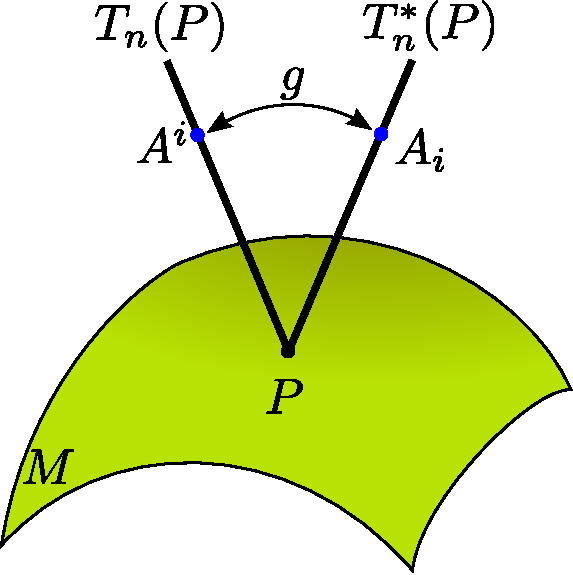
\psfig{file=fig/fig-espacios-tangente-y-cotangente.pdf,height=6cm,angle=0}}
\caption{El tensor m'etrico define una relaci'on uno a uno (isomorfismo) entre
los espacios tangente y cotangente en cada punto de la variedad.}
\label{5}
\end{figure}
\end{center}

El uso del tensor m'etrico para ``subir'' o ``bajar'' 'indices tambi'en es 'util para tensores de mayor rango. Por ejemplo, a partir del tensor de tipo $(^2_2)$, $T^{kl}{}_{i j}$, podemos definir el tensor de tipo $(^3_1)$:
\begin{equation}
T^{kl i}{}_j:=g^{im}T^{kl}{}_{mj},
\label{g10}
\end{equation}
etc.

\subsection{M'etrica inducida}
Considere una variedad $M$ de dimensi'on $n$ y una \textbf{subvariedad} $S$ de dimensi'on $d<n$. Entonces la m'etrica de $M$ \textit{induce la m'etrica sobre} $S$, ya que la distancia entre dos puntos arbitrarios de $S$ puede calcularse aplicando (o restringiendo) la distancia entre puntos infinitesimalmente pr'oximos de $M$ al caso particular de dos puntos infinitesimalmente pr'oximos de $S$. Si se usan coordenadas $x^i$ en (una vecindad de) $M$, y la subvariedad $S$ es definida por medio de una \textbf{parametrizaci'on} de la forma
\begin{equation}
x^i=x^i(y^a), \qquad a=1,\dots,d,
\end{equation}
donde $y^a$ son \textit{coordenadas sobre la subvariedad} $S$, entonces la diferencia de coordenadas de $M$ correspondiente a dos puntos infinitesimalmente pr'oximos de $S$ puede expresarse como
\begin{equation}
\left.dx^i\right|_{S}=\frac{\partial x^i}{\partial y^a}(x(y))\,dy^a.
\end{equation}
Con esto, podemos expresar el elemento de l'inea sobre $S$ como
\begin{align}
\left.dl^2\right|_{S}=&\left.g_{ij}(x)\right|_{S}\left.dx^i\right|_{S}\left.dx^j\right|_{S} \\
=& g_{ij}(x(y))\left(\frac{\partial x^i}{\partial y^a}dy^a\right)\left(\frac{\partial x^j}{\partial y^b}dy^b\right) \\
=& g_{ab}(y)dy^ady^b.
\end{align}
De esta forma, las componentes del tensor m'etrico inducido sobre $S$, en coordenadas $y^a$ est'a dadas por
\begin{equation}\marginnote{m'etrica inducida}\label{metind2}
\boxed{g_{ab}(y)= g_{ij}(x(y))\frac{\partial x^i}{\partial y^a}\frac{\partial x^j}{\partial y^b}.}
\end{equation}

Note que esta relaci'on \textit{no es} simplemente la usual ley de transformaci'on de las componentes del tensor m'etrico bajo una TGC, ya que $g_{ij}$ y $g_{ab}$ \textit{tienen dimensiones distintas} ($n$ y $d<n$ respectivamente) y son componentes de representan las \textit{m'etricas de dos variedades distintas} (pero relacionadas).

\subsection{Curvas geod'esicas}

Consideremos dos puntos $P$ y $Q$ en una variedad provista de m'etrica.
Se define la \textbf{geod'esica} como la curva \textit{de longitud m'inima  (extrema) entre} $P$ y $Q$.

Si $\cal C$ es una curva representada param'etricamente por
$x^i =x^i (\lambda)$, entonces $\cal C$ es una geod'esica entre $P$ y $Q$ si y
s'olo si\footnote{Suponemos, por simplicidad, pero sin perder generalidad, que el par'ametro $\lambda$ \textit{crece} desde $P$ a $Q$, de modo que en la integral $d\lambda>0$.}
\begin{equation}
L=\int_P^Qd\ell= \int_P^Q\sqrt{g_{ij}(x(\lambda))dx^idx^j}=\int_{\lambda i}^{\lambda_{f}}\sqrt{g_{ij}(x(\lambda))\frac{dx^i}{d\lambda}\frac{dx^j }{d\lambda}}\, d\lambda \label{gm1}
\end{equation}
es m'inima. Esto implica que su variaci'on respecto a peque\~nas desviaciones de la trayectoria geod'esica es nula:
\begin{equation}
\delta L=0. \label{gm2}
\end{equation}
La condici'on (\ref{gm2}) implica que las geod'esicas satisfacen las ecuaciones de Euler-Lagrange,
\begin{equation}
\frac{\delta L}{\delta x^i }=\frac{\partial \tilde{L}}{\partial x^i }-\frac
{d}{d\lambda}\left( \frac{\partial
\tilde{L}}{\partial\left(\frac{dx^i}{d\lambda}\right) }\right) =0,
\label{gm3}
\end{equation}
donde
\begin{equation}
\tilde{L}(x^i,\frac{dx^i}{d\lambda})=\sqrt{g_{ij}(x(\lambda))\frac{dx^i
}{d\lambda}\frac{dx^j }{d\lambda}}.
\label{gm4}
\end{equation}
De aqu'i, tenemos que
\begin{equation}
\frac{\partial\tilde{L}}{\partial x^k}=\frac{1}{2}(g_{lm}\dot{x}^l\dot{x}^m)^{-1/2}(\partial_k g_{ij})\dot{x}^i\dot{x}^j=\frac{1}{2\tilde{L}}(\partial_k g_{ij})\dot{x}^i\dot{x}^j,
\end{equation}
\begin{equation}
\frac{\partial\tilde{L}}{\partial \dot{x}^k}=\frac{1}{2}(g_{lm}\dot{x}^l\dot{x}^m)^{-1/2}(2g_{kj}\dot{x}^j)=\frac{1}{\tilde{L}}g_{kj}\dot{x}^j,
\end{equation}
\begin{equation}
\frac{d}{d\lambda}\left(\frac{\partial\tilde{L}}{\partial \dot{x}^k}\right)= -\frac{\dot{\tilde{L}}}{\tilde{L}^2}g_{kj}\dot{x}^j+\frac{1}{\tilde{L}}(\partial_l g_{kj})\dot{x}^j\dot{x}^l+\frac{1}{\tilde{L}}g_{kj}\ddot{x}^j.
\end{equation}
De esta forma, encontramos que
\begin{equation}
\frac{\delta L}{\delta x^i }=\frac{1}{2\tilde{L}}(\partial_k g_{ij})\dot{x}^i\dot{x}^j+\frac{\dot{\tilde{L}}}{\tilde{L}^2}g_{kj}\dot{x}^j-\frac{1}{\tilde{L}}(\partial_l g_{kj})\dot{x}^j\dot{x}^l-\frac{1}{\tilde{L}}g_{kj}\ddot{x}^j.
\end{equation}
Multiplicando por $\tilde{L}g^{ki}$ y reordenando t'erminos obtenemos
\begin{align}
\frac{\dot{\tilde{L}}}{\tilde{L}}\dot{x}^i &= \ddot{x}^i+g^{ik}(\partial_l g_{kj})\dot{x}^j\dot{x}^l-\frac{1}{2}(\partial_k g_{jl})\dot{x}^j\dot{x}^l \\
&= \ddot{x}^i+\frac{1}{2}g^{ik}\left(\partial_l g_{kj}+\partial_j g_{kl}-\partial_k g_{jl}\right)\dot{x}^j\dot{x}^l \\
&= \ddot{x}^i+\left\{ _{jl}^{\,i}\right\}\dot{x}^j\dot{x}^l.
\end{align}
Por lo tanto \eqref{gm3} es equivalente a 
\begin{equation}\marginnote{Ecuaci'on Geod'esicas}
\boxed{\frac{d^2x^i }{d\lambda^2}+\left\{ _{ j l}^{\, i}\right\}
\frac{dx^j }{d\lambda}\frac{dx^{ l}}{d\lambda}=f(\lambda)\frac{dx^{ i
}}{d\lambda},} \label{gm5}
\end{equation}
donde
\begin{equation}\marginnote{S'imbolos de Christoffel}
\boxed{\left\{ _{ jk}^{\,i}\right\}:=\frac{1}2g^{il}\left[
\partial_kg_{jl}+\partial_j g_{lk}-\partial_l g_{kj}\right] ,} \label{gm6}
\end{equation}
es llamado \textbf{s'imbolo de Christoffel}\footnote{En honor a Elwin Bruno Christoffel: 1829-1900, f'isico y matem'atico alem'an. Ver \url{http://es.wikipedia.org/wiki/Elwin_Bruno_Christoffel}.} (de segunda especie), y
\begin{equation}
f(\lambda):=\frac{\dot{\tilde{L}}}{\tilde{L}}=\frac{d\ }{d\lambda}\left(\ln\tilde{L}\right)=\frac{d\ }{d\lambda}\left(\ln\frac{d\ell}{d\lambda}\right) =\frac{\frac{d^2\ell}{d\lambda^2}}{\frac{d\ell}{d\lambda}}\label{efe}
\end{equation}
 es una funci'on que depende de la elecci'on del par'ametro $\lambda$ usado para parametrizar la curva. Note que aqu'i hemos impl'icitamente introducido una funci'on $\ell(\lambda)$, el largo de la curva desde el punto inicial $P_i$, dada por $\ell(\lambda):=\int_{\lambda_i}^\lambda \tilde{L}\,d\lambda$, de modo que $\tilde{L}=d\ell/ d\lambda$.

La relaci'on (\ref{efe}) determina la funci'on $f$ a partir de la relaci'on
entre la longitud propia de la curva y el par'ametro $\lambda$. De aqu'i es
directo verificar que un cambio de par'ametro $\lambda\to\lambda'$ implicar'a
un cambio en la funci'on $f$, de modo que
\begin{equation}\label{fpf}
f'=\left(\frac{d\lambda'}{d\lambda}\right)^{-1}\left[f-\frac{d\ }{d\lambda}\left(\ln\frac{d\lambda'}{d\lambda}\right)\right] .
\end{equation}
En efecto, como
\begin{equation}
\frac{d\ell}{d\lambda'}=\frac{d\ell}{d\lambda}\frac{d\lambda}{d\lambda'},
\end{equation}
\begin{equation}
\frac{d^2\ell}{d\lambda'^2}=\frac{d^2\ell}{d\lambda^2}\left(\frac{d\lambda}{d\lambda'}\right)^2+\frac{d\ell}{d\lambda}\frac{d^2\lambda}{d\lambda'^2},
\end{equation}
entonces
\begin{align}
f'&=\frac{\frac{d^2\ell}{d\lambda'^2}}{\frac{d\ell}{d\lambda'}} = \frac{\frac{d^2\ell}{d\lambda^2}\left(\frac{d\lambda}{d\lambda'}\right)^2+\frac{d\ell}{d\lambda}\frac{d^2\lambda}{d\lambda'^2}}{\frac{d\ell}{d\lambda}\frac{d\lambda}{d\lambda'}} =f\frac{d\lambda}{d\lambda'}+\frac{\frac{d^2\lambda}{d\lambda'^2}}{\frac{d\lambda}{d\lambda'}}
=f\frac{d\lambda}{d\lambda'}+\frac{d}{d\lambda'}\ln\left(\frac{d\lambda}{d\lambda'}\right),
\end{align}
que es equivalente a \eqref{fpf}.

Como consecuencia de la arbitrariedad de $\lambda$ es posible \textit{elegir par'ametros especiales que simplifiquen los c'alculos}. Por ejemplo, \textit{si $d\ell\neq 0$ sobre toda la geod'esica}, entonces podemos usar un \textbf{par'ametro af'in}, de la forma $\lambda_{\rm afin}:=\alpha\cdot \ell+\beta$, donde $\ell$ es la distancia \textit{sobre la curva} desde un punto de referencia hasta un punto arbitrario de ella, y adem'as $\alpha$ y $\beta$ son \textit{constantes} (escalares). En este caso (\ref{efe}) implica que $f=0$. Por simplicidad, usualmente se elige en estos casos la longitud (propia) de la curva ($\alpha=1$), de modo que la ecuaci'on de la geod'esica adopta la forma ``can'onica":
\begin{equation}\marginnote{Ec. Geod'esica c/param. af'in}
\boxed{\frac{d^2x^i }{d\ell^2}+\left\{ _{ j l}^{\, i}\right\}
\frac{dx^j }{d\ell}\frac{dx^{ l}}{d\ell}=0.} \label{gm7}%
\end{equation}

Por ejemplo, en el espacio euclidiano y en coordenadas cartesianas
$\left\{_{ j l}^{\, i}\right\}\overset{\ast}{=}0$, de modo que, de acuerdo con
(\ref{gm7}), las geod'esicas de este espacio son rectas con ecuaciones
$x^i (\ell)\overset{\ast}{=}x_0^i +\ell v_0^i $, con $x_0^i $ y $v_0^i$ constantes.

A partir de la ley de transformaci'on del tensor m'etrico puede verificarse f'acilmente que \textit{los s'imbolos de Christoffel no son componentes de un tensor bajo TGC's}, ya que
\begin{equation}
\overline{\left\{_{j k}^{\,\, i}\right\}}=\frac{\partial\bar{x}^i}{\partial x^l }\frac{\partial
x^p}{\partial\bar{x}^j }\frac{\partial x^q}{\partial\bar{x}^k }\,
\left\{_{p q}^{\,\, l}\right\} +\frac{\partial\bar{x}^i}{\partial x^l }\frac{\partial
^2x^l }{\partial\bar{x}^j \partial\bar{x}^k }. \label{dinv7}
\end{equation}

\subsection{Isometr'ias (simetr'ias de la m'etrica)}
\begin{center}
\begin{figure}[H]
\centerline{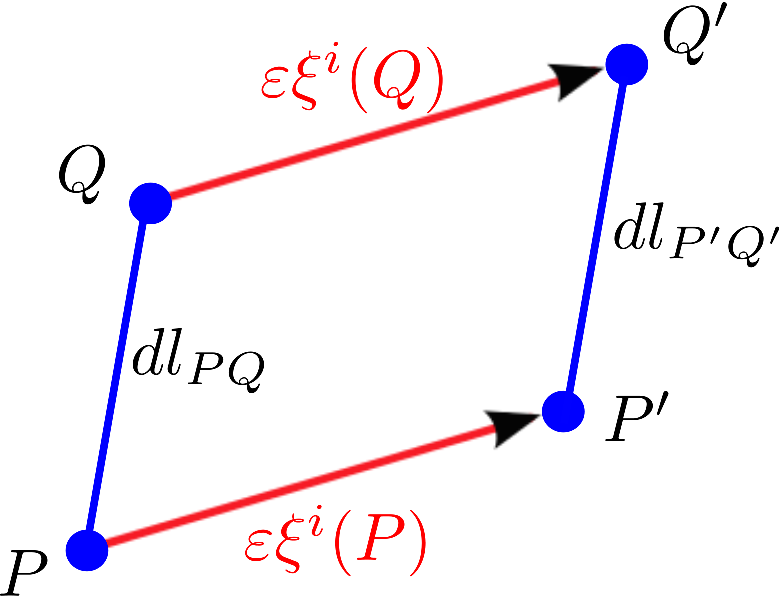
\psfig{file=fig/fig-Killing.pdf,height=5cm,angle=0}}
\caption{Trasladando puntos en la direcci'on $\xi^i(x)$.}
\label{fig:Killing}
\end{figure}
\end{center}
Las \textbf{isometr'ias} de una m'etrica (en caso de que existan) describen \textbf{direcciones de simetr'ia} de la m'etrica en (una regi'on de) la variedad, de una forma covariante, es decir, independiente del sistema de coordenadas usado. 

Sean $P$ y $Q$ dos puntos infinitesimalmente cercanos, con coordenadas $x^i$ y $x^i+dx^i$ respectivamente y $\xi^i=\xi^i(x)$ un campo vectorial (contravariante) definido en una vecindad que incluye a $P$ y $Q$. Como se muestra en la figura, podemos localizar dos nuevos puntos $P'$ y $Q'$ cuyas coordenadas est'an dadas por:%
\begin{align}
x^i(P')  & = x^i(P)+\varepsilon\,\xi^i(P)\label{is1},\\
x^i(Q')  & = x^i(Q)+\varepsilon\,\xi^i(Q), \label{is1b}
\end{align}
donde $\varepsilon$ es un par'ametro escalar infinitesimal. Los puntos $P'$ y $Q'$ son entonces los resultantes de ``trasladar'' los puntos $P$ y $Q$ en la direcci'on definida por el vector $\xi$. Se dice entonces que $\xi^i(x)$ describe una isometr'ia de la variedad, si para puntos arbitrarios $P$ y $Q$ se cumple que la distancia entre ellos es la misma que entre los puntos ``trasladados'' $P'$ y $Q'$, es decir, si
\begin{equation}
dl_{PQ}\stackrel{!}{=}dl_{P'Q'}  \label{is2}%
\end{equation}
o, m'as expl'icitamente,
\begin{align}
dl_{PQ}^2  &  =g_{ij}(P)(dx^i_{PQ})(dx^j_{PQ}) , \label{is3}\\
dl_{P'Q'}^2  &  =g_{ij}(P')(dx^i_{P'Q'})(dx^j_{P'Q'}) . \label{is4}
\end{align}
Usando (\ref{is1}), (\ref{is1b}) podemos escribir
\begin{align}
dx^i_{P'Q'} &= dx^i_{PQ}+\varepsilon\left[\xi^i(Q)-\xi^i(P)\right] \\
&= dx^i+\varepsilon\left[\xi^i(x+dx)-\xi^i(x)\right] \\
&= dx^i+\varepsilon \left[\partial_j\xi^i(x)\right]dx^j.
\end{align}
Con esta expresi'on (\ref{is4}) se reduce, a primer orden en $\varepsilon$, a
\begin{equation}
dl_{P'Q'}^2=g_{ij}dx^idx^j+\varepsilon\left[g_{ij}dx^idx^k\partial_k\xi^i
+g_{ij}dx^kdx^j\partial_k\xi^i+\xi^kdx^idx^j\partial_kg_{ij}\right],  \label{is5}
\end{equation}
donde ahora todos los campos est'an evaluados en el punto $P$, de coordenadas $x^i$.
Cambiando adecuadamente los 'indices de suma, la expresi'on (\ref{is5}) toma la forma
\begin{equation}
dl_{P'Q'}^2=g_{ij}dx^idx^j+\varepsilon\left[g_{ik}\partial_j\xi^k
+g_{kj}\partial_i\xi^k+\xi^k\partial_kg_{ij}\right] dx^idx^j,
\label{is6}%
\end{equation}
de modo que la condici'on (\ref{is2}) es equivalente a
\begin{equation}\marginnote{Ecuaci'on de Killing}
\boxed{g_{ik}\partial_j\xi^k+g_{kj}\partial_i\xi^k+\xi^k\partial_kg_{ij}=0.} \label{is8}
\end{equation}
ya que $\varepsilon$, $dx^i$ son infinitesimales, pero arbitrarios.

La ecuaci'on\footnote{M'as exactamente, las $n(n+1)/2$ ecuaciones.} diferencial parcial lineal (\ref{is8}) es la condici'on que debe satisfacer el campo $\xi^i$ para que describa una isometr'ia. Las soluciones (no nulas) son llamadas \textbf{vectores de Killing}\footnote{Wilhelm Karl Joseph Killing (1847-1923): matem'atico alem'an. Ver \url{http://en.wikipedia.org/wiki/Wilhelm_Killing}  \textbf{$\leftarrow$ se necesita traducci'on al espa\~nol de esto!}.}.

\subsubsection{Plano euclideano}

En el plano euclidiano y en coordenadas cartesianas, $x^i=(x,y)$, la
m'etrica es $g_{ij}\overset{\ast}{=}\delta_{ij}$.
%Luego, de la ecuaci'on (\ref{gm6}) tenemos que los s'imbolos de Christoffel son
%nulos. y por lo tanto la curvatura tambi'en es nula.
%
%La ecuaci'on de las geod'esicas (\ref{gm7}) es%
%\begin{equation}
%\frac{d^2x^i}{d\ell^2}=0. %
%\end{equation}
%Por lo tanto, las geod'esicas en el plano son rectas.
En este caso la ecuaci'on (\ref{is8}) se reduce a:
\begin{align}
\delta_{ik}\partial_j\xi^k+\delta_{kj}\partial_i\xi^k  &  =0,\label{isej1}\\
\partial_j\xi_i+\partial_i\xi_j  &  =0. \nonumber
\end{align}

Escribimos expl'icitamente estas ecuaciones:%
\begin{align}
\partial_1\xi^1+ & \partial_1\xi^1= 0, \label{isej2}\\
\partial_1\xi^2+ & \partial_2\xi^1= 0, \label{isej3} \\
\partial_2\xi^2+ & \partial_2\xi^2= 0.  \label{isej4}
\end{align}
De (\ref{isej2}) y de (\ref{isej4}) se obtiene respectivamente que $\xi
^1=\xi^1(y)$ y $\xi^2=\xi^2(x)$. De este modo la ecuaci'on (\ref{isej3}) toma la forma:
\begin{equation}
\frac{d\xi^2}{dx}+\frac{d\xi^1}{dy}=0.  \label{isej5}%
\end{equation}
Usando el hecho de que $x$ e $y$ son coordenadas independientes, vemos que
esta ecuaci'on se satisface si y s'olo si:
\begin{align}
\frac{d\xi^1}{dy}  &  =\alpha=\text{cte.},\label{isej6}\\
\frac{d\xi^2}{dx}  &  =-\alpha, \nonumber
\end{align}
de modo que:
\begin{equation}
\xi^1 =\alpha y+\beta, \qquad
\xi^2 =-\alpha x+\gamma. \label{isej7}
\end{equation}
Esta soluci'on se puede expresar como combinaci'on lineal de tres
soluciones linealmente independientes:
\begin{align}
\xi^i  &  =\left(  \xi^1,\xi^2\right)  \\
& =\left(  \alpha y+\beta,-\alpha x+\gamma\right) \\
  &  =\alpha\left(  y,-x\right)  +\beta\left(  1,0\right)
+\gamma\left(  0,1\right)  \\
 &  =\alpha\,\xi_{(1)}^i+\beta\,\xi_{(2)}^i+\gamma\,\xi_{(3)}^i, \nonumber
\end{align}
donde
\begin{align}
\xi_{(1)}^i  &  :=\left(  y,-x\right)  ,\\
\xi_{(2)}^i  &  :=\left(  1,0\right)  ,\\
\xi_{(3)}^i  &  :=\left(  0,1\right)  .
\end{align}
\begin{center}
\begin{figure}[H]
\centerline{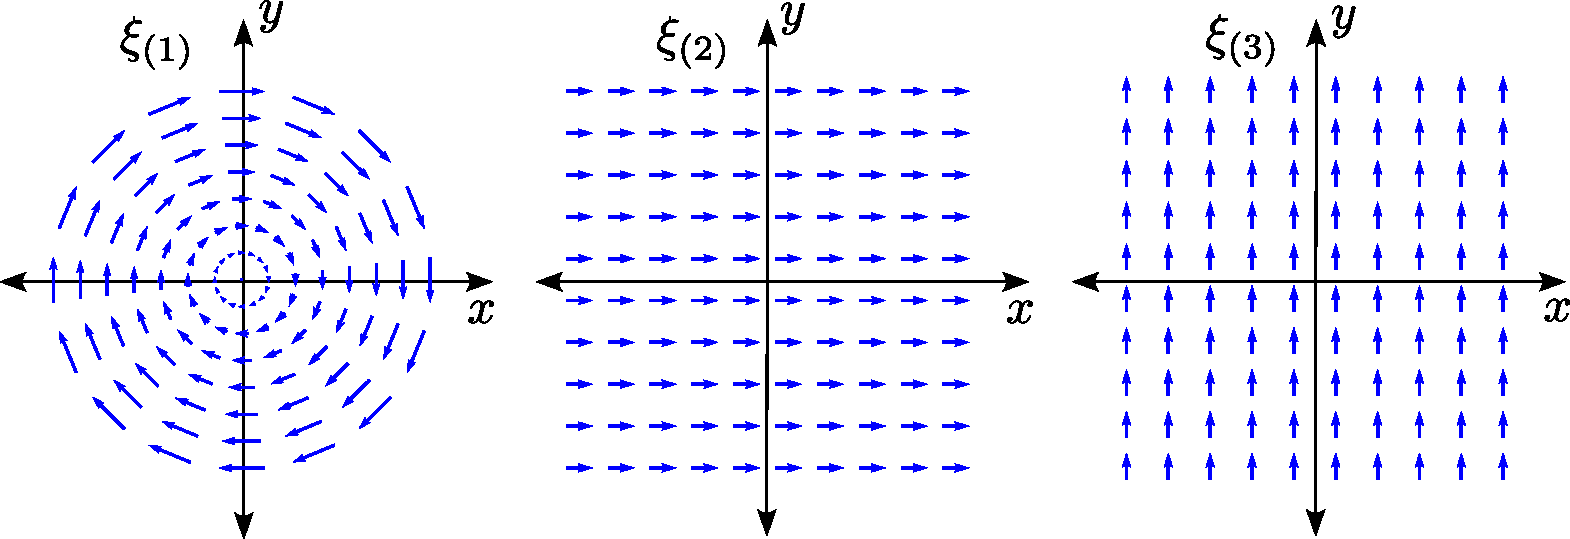
\psfig{file=fig/fig-Killing-E2.pdf,height=4cm,angle=0}}
\caption{Vectores de Killing en el plano euclideano bidimensional.}
\label{KE2}
\end{figure}
\end{center}
Los tres campos independientes $\xi^i_{(a)}$, $a=1,2,3$ son representados en la figura \ref{KE2}. Los vectores $\xi^i_{(1)}$ y $\xi^i_{(2)}$ corresponden a \textit{traslaciones} a lo largo de los ejes $x$ e $y$ respectivamente, mientras que $\xi^i_{(1)}$ a \textit{rotaciones} respecto al origen. Cualquier combinaci'on lineal (a coeficientes constantes) de estos tres vectores b'asicos define una direcci'on de simetr'ia del espacio Euclideano bidimensional.
\subsubsection{Esfera unitaria}

Consideremos como segundo ejemplo la m'etrica que el espacio euclidiano
tridimensional $E_{3}$ induce sobre la esfera unitaria. Sabemos que en
coordenadas cartesianas la m'etrica de $E_{3}$ es $g_{ij}=\delta_{ij}$ y la restricci'on a los puntos de la esfera es:
\begin{align}
x^1  &  =\sen\theta\cos\varphi,\\
x^2  &  =\sen\theta\sen\varphi,\\
x^{3}  &  =\cos\theta,
\end{align}
de modo que las coordenadas sobre la esfera son $\theta$ y $\varphi$. Usando
(\ref{metind2}) para calcular la m'etrica inducida, obtenemos
\begin{equation}
g_{ab}=\left(
\begin{array}[c]{cc}
1 & 0\\
0 & \sen^2\theta
\end{array}\right) ,  \label{ind7}
\end{equation}
donde $a,b=\theta,\varphi$. Usando (\ref{gm6}) obtenemos que las componentes no
nulas del s'imbolo de Christoffel son:
\begin{align}
\left\{  _{\varphi\varphi}^{\ \theta}\right\}  &  =-\sen\theta\cos\theta,\label{ind8}\\
\left\{  _{\theta\varphi}^{\, \varphi}\right\}   &  =\left\{  _{\varphi\theta}^{\,\varphi}\right\}  =\cot\theta.
\end{align}
%De este modo, se obtiene directamente que las ecuaciones para las
%geod'esicas sobre la esfera son:%
%\begin{align}
%\frac{d^2\theta}{d\ell^2}-\sen\theta\cos\theta\left(\frac{d\varphi}{d\ell}\right)^2  &  =0,\label{ind9}\\
%\frac{d^2\varphi}{d\ell^2}+2\cot\theta\frac{d\theta}{d\ell}\frac{d\varphi}{d\ell}  &  =0.
%\end{align}
%Tambi'en, mediante un c'alculo directo, encontramos que las componentes
%no nulas de la curvatura de la esfera son:%
%\begin{align}
%R_{\phi\theta\phi}^{\theta}  &  =-R_{\phi\phi\theta}^{\theta}=\sin^2%
%\theta,\label{ind10}\\
%R_{\theta\theta\phi}^{\phi}  &  =-R_{\theta\phi\theta}^{\phi}=-1. %
%\nonumber
%\end{align}

El sistema de ecuaciones para los vectores de Killing sobre la esfera unitaria,
seg\'{u}n (\ref{is8}) es:
\begin{align}
g_{\theta\theta}\partial_\theta\xi^\theta+g_{\theta\theta}\partial_\theta\xi^\theta +\xi^a\partial_ag_{\theta\theta}  &  =0,\label{isej12}\\
g_{\theta\theta}\partial_\varphi\xi^\theta+g_{\varphi\varphi}\partial_\theta\xi^\varphi +\xi^a\partial_ag_{\theta\varphi}  &  =0, \\
g_{\varphi\varphi}\partial_\varphi\xi^\varphi+g_{\varphi\varphi}\partial_\varphi\xi^\varphi +\xi^a\partial_ag_{\varphi\varphi}  &  =0.
\end{align}
Luego:
\begin{align}
\partial_\theta\xi^\theta  &  =0,\label{isej13}\\
\partial_\varphi\xi^\theta+\sen^2\theta\,\partial_\theta\xi^\varphi  &  =0, \\
2\sen^2\theta\,\partial_\varphi\xi^\varphi+\xi^\theta\partial_\theta(\sen^2\theta)  & =0.
\end{align}
La primera ecuaci'on nos dice que $\xi^\theta=\xi^\theta(\varphi)$, de modo que la
segunda y tercera ecuaci'on nos queda:
\begin{align}
\partial_\varphi\xi^\theta+\sen^2\theta\,\partial_\theta\xi^\varphi  &
=0,\label{isej14}\\
\sen\theta\,\partial_\varphi\xi^\varphi+\xi^\theta\cos\theta  &  =0.
\end{align}
Se puede verificar, reemplazando directamente en estas ecuaciones, que el
sistema tiene por soluci'on:
\begin{equation}
\xi^a=\alpha\,\xi^a_{(1)} +\beta\,\xi^a_{(2)} +\gamma\,\xi^a_{(3)}
,\label{isej15}
\end{equation}
con
\begin{eqnarray}
\xi^a_{(1)} &=&(\sen\varphi, \cot\theta\cos\varphi ), \\
\xi^a_{(2)} &=&(\cos\varphi,-\cot\theta\sen\varphi) , \\
\xi^a_{(3)} &=&(0,1).
\end{eqnarray}

\begin{center}
\begin{figure}[H]
\centerline{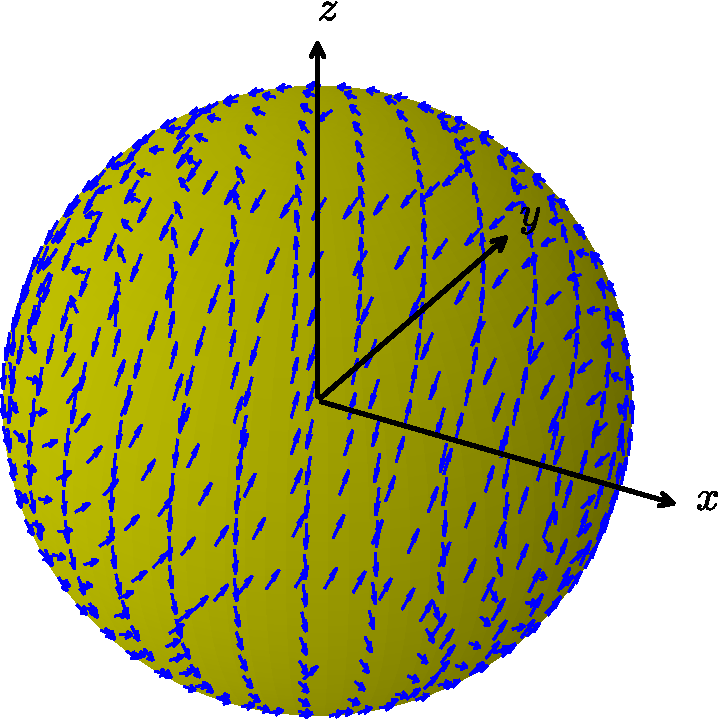
\psfig{file=fig/fig-KS2x.pdf,height=4cm,angle=0}\hfill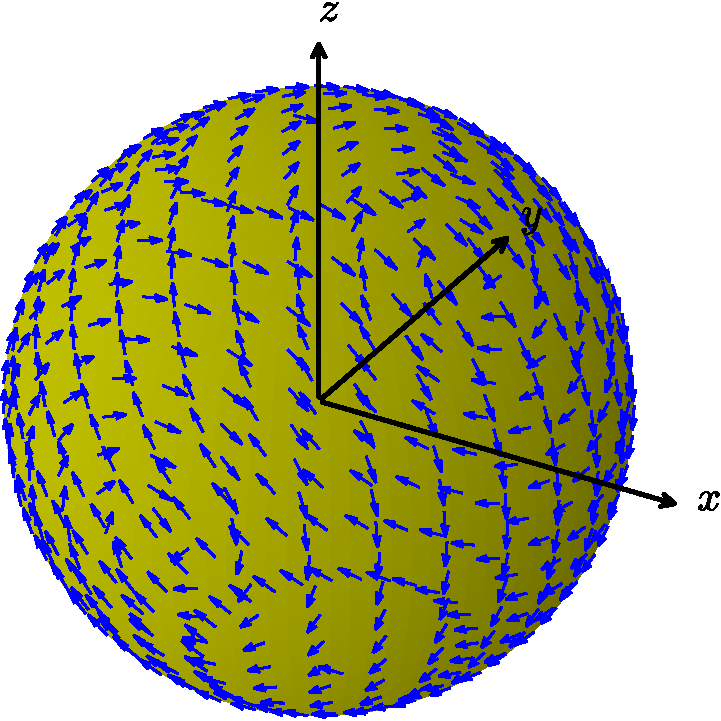
\psfig{file=fig/fig-KS2y.pdf,height=4cm,angle=0}\hfill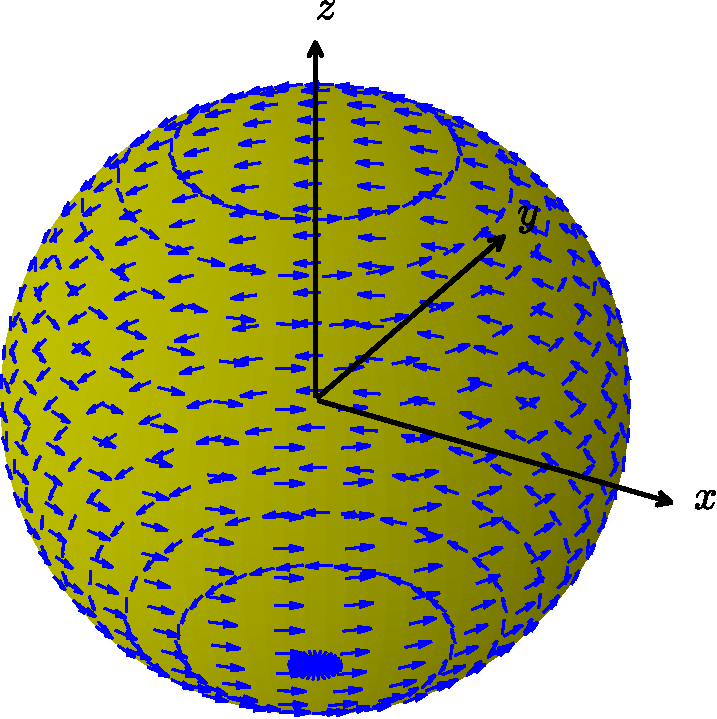
\psfig{file=fig/fig-KS2z.pdf,height=4cm,angle=0}}
\caption{Vectores de Killing sobre la esfera: 
$\xi^a_{(1)}$, $\xi^a_{(2)}$ y $\xi^a_{(3)}$ respectivamente.}
\label{KS2}
\end{figure}
\end{center}

\paragraph{Teorema:} El n'umero m'aximo de vectores de Killing independientes que una variedad de dimensi'on $n$ puede admitir es $n(n+1)/2$ *** Agregar ref. ***

***
\subsection{Coodenadas adaptadas a una isometr'ia}

Definimos una coordenada, por ejemplo, $x^1$, a lo largo de las l'ineas integrales del campo $\xi$, es decir, tal que los vectores tangentes a las l'ineas coordenadas de $x^1$ son paralelos a $\xi$. Esto implica que en el SC adaptado 
\begin{equation}
\xi^i\stackrel{*}{=}(\xi^1,0,\cdots,0).
\end{equation}
Siempre es posible definir la coordenada $x^1$ (en particular, qu'e tan r'apido var'ia 'esta sobre las curvas integrales de $\xi$) de modo que
\begin{equation}
\xi^i\stackrel{*}{=}(1,0,\cdots,0).
\end{equation}
Entonces, si $\xi$ es un vector de Killing, la ecuaci'on \eqref{is8} implica que
\begin{equation}
\partial_1g_{ij}\stackrel{*}{=}0,
\end{equation}
es decir, que en sistema de coordenadas adaptado al vector de Killing $\xi$ la m'etrica no depende de la coordenada adaptada $x^1$.

\subsection{Vectores de Killing y operadores diferenciales}
\begin{equation}
\hat{\xi}:=\xi^i\partial_i
\end{equation}

\section{Conexi'on, derivadas covariantes y transporte paralelo}

\subsection{Derivada parcial de campos tensoriales}

Salvo en el caso de un escalar, \textit{la derivada de las componentes de un tensor no define un nuevo tensor bajo TGC's}. Esto puede entenderse como una consecuencia del hecho que la definici'on de la derivada parcial de un tensor involucra (el l'imite) de la sustracci'on de tensores \textit{en puntos distintos}.

En efecto, veamos c'omo transforman las derivadas parciales $\partial_i
A_j:={\partial A_j}/{\partial x^i}$ de un vector covariante $A_i$:
\begin{equation}
\bar{\partial}_i\bar{A}_j=\frac{\partial \bar{A}_j}{\partial
\bar{x}^i}=\frac{\partial }{\partial \bar{x}^i}\left(\frac{\partial x^k
}{\partial\bar{x}^j }A_k \right)
=\frac{\partial x^k }{\partial\bar{x}^j }\frac{\partial x^l }{\partial\bar{x}^i}
\partial_l A_k +\frac{\partial^2 x^k }{\partial\bar
{x}^i \partial\bar{x}^j }A_k . \label{ord2}
\end{equation}
Vemos que la derivada parcial de un vector covariante se comporta como un tensor tipo $(_2^0)$ \textit{excepto por el segundo t'ermino}. La ley de
transformaci'on es lineal, pero inhomog'enea, lo que implica que si las
derivadas de un vector se anulan en un SC entonces 'estas no se anulan
necesariamente en otro.

Una consecuencia importante de este hecho es que, \textit{sin introducir elementos adicionales definidos sobre la variedad}, no existe un criterio \textit{independiente de coordenadas} de cu'ando un tensor es constante sobre (una regi'on de) la variedad. Esto se debe a que, como se deduce de la expresi'on \eqref{ord2}, aunque las componentes de un tensor sean iguales en dos puntos (o en una regi'on) de la variedad en alg'un SC ($x$, de modo que $\partial_iA_j=0$) en otros SC's ($\bar{x}$) 'este no ser'a el caso: $\bar{\partial}_i\bar{A}_j\neq 0$.
 
Lo mismo ocurre para tensores de distinto tipo. Por ejemplo, la ley de transformaci'on de un tensor tipo ($_2^0$) es:
\begin{equation}
\bar{A}_{jk}=\frac{\partial x^l}{\partial\bar{x}^j} \frac{\partial x^m}{\partial\bar{x}^k}A_{lm}. \label{ord3}
\end{equation}
Luego, sus derivadas parciales transforman bajo una TGC de la forma siguiente:
\begin{equation}
\bar{\partial}_i\bar{A}_{jk}=\frac{\partial x^l}{\partial\bar{x}^j} 
\frac{\partial x^m}{\partial\bar{x}^k} \frac{\partial x^n}{\partial \bar{x}^i}\,\partial_nA_{lm}+\left(
\frac{\partial^2 x^l}{\partial\bar{x}^i\partial\bar{x}^j} \frac{\partial x^m}{\partial\bar{x}^k} 
+\frac{\partial x^l}{\partial\bar{x}^j}\frac{\partial^2 x^m}{\partial\bar{x}^i\partial\bar{x}^k}\right) A_{lm}. \label{ord4}
\end{equation}

Vemos que los dos 'ultimos t'erminos en (\ref{ord4}) son lineales en las
componentes (no derivadas) del tensor original y son tambi'en lineales en las segundas derivadas del cambio de coordenadas. Estos t'erminos hacen que la ley de transformaci'on de las derivadas parciales difiera de la ley correspondiente a un tensor.

\subsubsection{Excepciones*}
Existen, sin embargo, ciertas combinaciones particulares de derivadas parciales que s'i son tensores. Por ejemplo, el ``rotor'' de un campo vectorial covariante $A_k $, $\partial_k A_i-\partial_iA_k $, es un tensor tipo ($_2^0$), ya que
\begin{align}
\bar{A}_k  & =\frac{\partial x^l}{\partial\bar{x}^k} A_l ,\label{ord6}\\
\bar{\partial}_i\bar{A}_k  & =\frac{\partial x^l}{\partial\bar{x}^k} 
\frac{\partial x^m}{\partial\bar{x}^i}\, \partial_mA_l +
\frac{\partial^2 x^l}{\partial\bar{x}^i\partial\bar{x}^k}\, A_l ,\\
\bar{\partial}_k \bar{A}_i & =\frac{\partial x^l}{\partial\bar{x}^i}
\frac{\partial x^m}{\partial\bar{x}^k}\, \partial_mA_l +
\frac{\partial^2 x^l}{\partial\bar{x}^k\partial\bar{x}^i}\, A_l ,\\
\end{align}
y por lo tanto
\begin{equation}
 \bar{\partial}_i\bar{A}_k -\bar{\partial}_k \bar{A}_i =\frac{\partial x^l}{\partial\bar{x}^k} \frac{\partial x^m}{\partial\bar{x}^i} \left( \partial_m A_l -\partial_l A_m\right) .
\end{equation}
De este modo, $\left(\partial_iA_j -\partial_j A_i\right)$ define un tensor
antisim'etrico de tipo ($_2^0$).

% \item La divergencia c'iclica de cualquier tensor antisim'etrico tipo
% ($_2^0$) es un tensor antisim'etrico tipo ($_{3}^0$). En efecto, sea
% $T_{ik}$ un tensor antisim'etrico. Entonces:
% \begin{equation}
% \bar{T}_{ik}=\frac{\partial x^l}{\partial\bar{x}^i} \frac{\partial x^m}{\partial\bar{x}^k} %
% T_{lm}. \label{ord8}%
% \end{equation}
% Queremos mostrar que \ $\partial_jT_{ik}+\partial_iT_{kj}+\partial
% _k T_{ji}$ es un tensor. Para esto calculemos dichos sumandos a partir de
% (\ref{ord8}):
% \begin{equation}
% \bar{\partial}_j\bar{T}_{ik}=\frac{\partial x^l}{\partial\bar{x}^i} \bar{\partial
% }_k x^m \bar{\partial}_jx^n\partial_nT_{lm}+\left(
% \bar{\partial}_j\frac{\partial x^l}{\partial\bar{x}^i} \,\frac{\partial x^m}{\partial\bar{x}^k} %
% +\frac{\partial x^l}{\partial\bar{x}^i} \,\bar{\partial}_j\frac{\partial x^m}{\partial\bar{x}^k} \right)
% T_{lm}, \label{ord9}%
% \end{equation}%
% \begin{equation}
% \bar{\partial}_i\bar{T}_{kj}=\frac{\partial x^l}{\partial\bar{x}^k} \bar{\partial
% }_jx^m \frac{\partial x^n}{\partial\bar{x}^i}\partial_nT_{lm}+\left(
% \bar{\partial}_i\frac{\partial x^l}{\partial\bar{x}^k} \,\bar{\partial}_jx^m %
% +\frac{\partial x^l}{\partial\bar{x}^k} \,\bar{\partial}_i\bar{\partial}_jx^m \right)
% T_{lm}, \label{ord10}%
% \end{equation}%
% \begin{equation}
% \bar{\partial}_k \bar{T}_{ji}=\frac{\partial x^l}{\partial\bar{x}^j} \bar{\partial
% }_ix^m \bar{\partial}_k x^n\partial_nT_{lm}+\left(
% \bar{\partial}_k \frac{\partial x^l}{\partial\bar{x}^j} \,\frac{\partial x^m}{\partial\bar{x}^i} %
% +\frac{\partial x^l}{\partial\bar{x}^j} \,\bar{\partial}_k \frac{\partial x^m}{\partial\bar{x}^i} \right)
% T_{lm}. \label{ord11}%
% \end{equation}
% Si se suman los tres t'erminos, se combinan adecuadamente los 'indices
% mudos $l$, $m$ y $n$, y se usan las propiedades de antisimetr'ia de $T$,
% se obtiene:
% \begin{equation}
% \bar{\partial}_j\bar{T}_{ik}+\bar{\partial}_i\bar{T}_{kj}+\bar{\partial
% }_k \bar{T}_{ji}=\frac{\partial x^l}{\partial\bar{x}^i} \frac{\partial x^m}{\partial\bar{x}^k} \text{
% }\bar{\partial}_jx^n\left( \partial_nT_{lm}+\partial_l T_{mn}%
% +\partial_mT_{nl}\right), \label{ord12}%
% \end{equation}
% lo cual prueba que la divergencia c'iclica de un tensor antisim'etrico
% tipo ($_2^0$) es un tensor antisim'etrico tipo ($_{3}^0$).


Todo esto no es suficiente para establecer un an'alisis tensorial
exhaustivo sobre una variedad. Una (aparentemente simple) pregunta a'un no tiene respuesta: \textquestiondown Qu'e condici'on caracteriza un campo vectorial
\textit{constante}? Claramente la respuesta \underline{no es}
$\partial_iA_j=0$, pues esta condici'on no es independiente del SC usado. De hecho, sin estructuras adicionales definidas sobre la variedad, el concepto de ``campo vectorial constante"\, simplemente no est'a definido. La estructura adicional que permite formular 'este y otros conceptos, por ejemplo el de derivada covariante, es llamada \textbf{conexi'on}.

\subsection{Conexi'on y derivada covariante de tensores}

\textbf{Definici'on:} Llamamos \textbf{conexi'on}\footnote{Tambi'en llamada \textbf{conexi'on af'in} o \textbf{afinidad}.}, $\Gamma$, \textit{a un arreglo de} $n^3$ \textit{cantidades definidas en cada punto de la variedad para las cuales:}
\begin{itemize}
\item Suponemos un conjunto de valores dados en cada SC particular y,
\item Cambian sus valores bajo una TGC de acuerdo a la siguiente ley de transformaci'on:
\begin{equation}\marginnote{Conexi'on}
\bar{\Gamma}_{\ jk}^i=\frac{\partial\bar{x}^i}{\partial x^l }\frac{\partial
x^p}{\partial\bar{x}^j }\frac{\partial x^q}{\partial\bar{x}^k }\,
\Gamma_{\ pq}^l +\frac{\partial\bar{x}^i}{\partial x^l }\frac{\partial
^2x^l }{\partial\bar{x}^j \partial\bar{x}^k }. \label{dinv72}
\end{equation}
\end{itemize}
A partir de una conexi'on y de un campo vectorial (covariante) es posible definir la siguiente combinaci'on, que es un tensor bajo TGC's:
\begin{equation}
\boxed{\nabla_iA_j:=\partial_iA_j-\Gamma_{\ ji}^kA_k.}
\label{dinv6}
\end{equation}
El tensor $\nabla_iA_j$ es llamado la \textbf{derivada covariante} de $A_j$ \textit{con respecto a la conexi'on} $\Gamma$. Se debe notar que $\Gamma$ est'a definida \textit{sobre} nuestra variedad y puede ser concebida,\textit{ en general}, como un objeto geom'etrico \textit{no necesariamente relacionado con una  m'etrica}.


Es simple verificar a partir de \eqref{ord2} y \eqref{dinv6} que $\nabla_iA_j$ es efectivamente covariante (es decir, un tensor), si suponemos que las componentes de $\Gamma$ transforman de acuerdo a \eqref{dinv72}.

Note que el segundo t'ermino del lado derecho de \eqref{dinv72} es independiente de $\Gamma$ y depende entonces s'olo de la transformaci'on de coordenadas. Esta es la propiedad implica que una conexi'on $\Gamma$ no sea nula en todo SC, a'un cuando puede serlo en algunos. Otra consecuencia de la ley de transformaci'on \eqref{dinv72} es que si \textit{dos conexiones}, $\Gamma$ y $\hat{\Gamma}$, definidas en la misma variedad, entonces \textit{su diferencia es un tensor}. En efecto, bajo una TGC se tiene que
\begin{align}
\bar\Gamma_{\ ik}^n-\hat{\overline{\Gamma}}{}^n_{\ ik} & =\frac{\partial
\bar{x}^n}{\partial x^l }\frac{\partial x^r}{\partial\bar{x}^i }
\frac{\partial x^s}{\partial\bar{x}^k }\,\Gamma_{\ rs}^l +\frac{\partial
\bar{x}^n}{\partial x^l }\frac{\partial^2 x^l }{\partial\bar{x}^i \partial\bar{x}^k }-\frac{\partial\bar{x}^n}{\partial x^l }
\frac{\partial x^r}{\partial\bar{x}^i }\frac{\partial x^s}{\partial
\bar{x}^k }\,\hat{\Gamma}_{\ rs}^l -\frac{\partial\bar{x}^n}{\partial x^l}\frac{\partial^2 x^l }{\partial\bar{x}^i \partial\bar{x}^k}\label{dinv8}\\
& =\frac{\partial
\bar{x}^n}{\partial x^l }\frac{\partial x^r}{\partial\bar{x}^i }
\frac{\partial x^s}{\partial\bar{x}^k }\left( \Gamma_{\ rs}^l
-\hat{\Gamma}_{\ rs}^l \right) .\nonumber
\end{align}
Luego, la diferencia $\Gamma_{jk}^i -\hat{\Gamma}_{jk}^i $ es un tensor. Equivalentemente, la suma de una conexi'on y un tensor de tipo $(_2^1)$ es una nueva conexi'on.

% Veamos qu'e sucede si sumamos dos afinidades, $\Gamma_{lm}^k $ y
% $\hat{\Gamma}_{lm}^k $:
% \begin{align}
% \bar\Gamma_{\ ik}^n+\overline{\hat{\Gamma}}_{ik}^n & =\frac{\partial
% \bar{x}^n}{\partial x^l }\frac{\partial x^r}{\partial\bar{x}^i }%
% \frac{\partial x^s}{\partial\bar{x}^k }\Gamma_{\ rs}^l +\frac{\partial
% \bar{x}^n}{\partial x^l }\frac{\partial^2 x^l }{\partial\bar{x}%
% ^i \partial\bar{x}^k }+\frac{\partial\bar{x}^n}{\partial x^l }%
% \frac{\partial x^r}{\partial\bar{x}^i }\frac{\partial x^s}{\partial
% \bar{x}^k }\hat{\Gamma}_{rs}^l +\frac{\partial\bar{x}^n}{\partial x^l %
% }\frac{\partial^2 x^l }{\partial\bar{x}^i \partial\bar{x}^k %
% },\label{dinv9}\\
% \bar\Gamma_{\ ik}^n+\overline{\hat{\Gamma}}_{ik}^n & =\frac{\partial
% \bar{x}^n}{\partial x^l }\frac{\partial x^r}{\partial\bar{x}^i }%
% \frac{\partial x^s}{\partial\bar{x}^k }\left( \Gamma_{\ rs}^l +\hat{\Gamma
% }_{rs}^l \right) +2\frac{\partial\bar{x}^n}{\partial x^l }\frac
% {\partial^2 x^l }{\partial\bar{x}^i \partial\bar{x}^k }.\nonumber
% \end{align}
%
%
% Luego la suma de dos afinidades no es una afinidad. Pero si $\lambda$ y $\mu$
% son n'umeros tales que $\lambda+\mu=1$ entonces tenemos:
% \begin{align}
% \lambda\bar\Gamma_{\ ik}^n+\mu\overline{\hat{\Gamma}}_{ik}^n &
% =\lambda\frac{\partial\bar{x}^n}{\partial x^l }\frac{\partial x^r%
% }{\partial\bar{x}^i }\frac{\partial x^s}{\partial\bar{x}^k }\Gamma
% _{rs}^l +\lambda\frac{\partial\bar{x}^n}{\partial x^l }\frac{\partial
% ^2x^l }{\partial\bar{x}^i \partial\bar{x}^k }+\mu\frac{\partial\bar
% {x}^n}{\partial x^l }\frac{\partial x^r}{\partial\bar{x}^i }%
% \frac{\partial x^s}{\partial\bar{x}^k }\hat{\Gamma}_{rs}^l +\mu
% \frac{\partial\bar{x}^n}{\partial x^l }\frac{\partial^2 x^l }%
% {\partial\bar{x}^i \partial\bar{x}^k }\label{dinv10}\\
% \lambda\bar\Gamma_{\ ik}^n+\mu\overline{\hat{\Gamma}}_{ik}^n &
% =\frac{\partial\bar{x}^n}{\partial x^l }\frac{\partial x^r}{\partial
% \bar{x}^i }\frac{\partial x^s}{\partial\bar{x}^k }\left( \lambda
% \Gamma_{\ rs}^l +\mu\hat{\Gamma}_{rs}^l \right) +\lambda\frac{\partial\bar
% {x}^n}{\partial x^l }\frac{\partial^2 x^l }{\partial\bar{x}^i %
% \partial\bar{x}^k }+\mu\frac{\partial\bar{x}^n}{\partial x^l }%
% \frac{\partial^2 x^l }{\partial\bar{x}^i \partial\bar{x}^k }\nonumber\\
% \lambda\bar\Gamma_{\ ik}^n+\mu\overline{\hat{\Gamma}}_{ik}^n &
% =\frac{\partial\bar{x}^n}{\partial x^l }\frac{\partial x^r}{\partial
% \bar{x}^i }\frac{\partial x^s}{\partial\bar{x}^k }\left( \lambda
% \Gamma_{\ rs}^l +\mu\hat{\Gamma}_{rs}^l \right) +\frac{\partial\bar{x}^n%
% }{\partial x^l }\frac{\partial^2 x^l }{\partial\bar{x}^i \partial\bar
% {x}^k }.\nonumber
% \end{align}
%
%
% Por lo tanto, $\lambda\Gamma_{\ rs}^l +\mu\hat{\Gamma}_{rs}^l $ es una
% afinidad si y s'olo si $\lambda+\mu=1$.

 La noci'on de derivada covariante introducida en (\ref{dinv6}) no es un concepto intr'inseco, ``natural'' de una variedad, sino que est'a definida a partir de una conexi'on, la cual debe ser indicada. Adem'as, es posible introducir m'as que una conexi'on sobre la misma variedad, por lo que es en general necesario distinguir entre las derivadas definidas con respecto a distintas conexiones.

Se extender'a ahora la noci'on de derivada covariante a tensores de distinto tipo. Existen distintas formas de motivar la definici'on de derivadas covariantes de tensores de tipo arbitrario. Una manera simple es  \textit{asumiendo} que la derivaci'on covariante satisface:
\begin{itemize}
\item[i)] la usual regla de la derivaci'on de un producto (regla de
Leibniz\footnote{En honor de Gottfried Leibniz: 1646-1716, fil'osofo, matem'atico, jurista, bibliotecario y pol'itico alem'an. Ver \url{http://es.wikipedia.org/wiki/Gottfried_Leibniz}.}) cuando se aplica al producto de tensores y,
\item[ii)] que la derivada covariante de un escalar coincide con la usual derivaci'on parcial.
\end{itemize}

A partir de estas propiedades es posible deducir la forma de la derivada covariante de cualquier cantidad tensorial. Por ejemplo, la derivada $\nabla_iB^j$ de un vector contravariante $B^j$ puede encontrarse aplicando las propiedades arriba descritas al escalar $A_k B^k $, donde $A_k$ son las componentes de un vector covariante (auxiliar). En efecto, la propiedad ii) implica que
\begin{equation}
\nabla_i\left( A_k B^k\right)=\partial_i\left( A_k B^k \right).\label{dinv12}
\end{equation}
Usando ahora la propiedad i), es decir, la regla de Leibniz podemos escribir
\begin{equation}
A_k (\nabla_iB^k)+(\nabla_i A_k)B^k = A_k (\partial_iB^k) +(\partial_iA_k)B^k .
\end{equation}
Finalmente, usando \eqref{dinv6} encontramos que
\begin{equation}
A_k (\nabla_iB^k) +\left(\partial_iA_k-\Gamma_{\ ki}^jA_j\right) B^k=A_k (\partial_iB^k) +(\partial_iA_k)B^k 
\end{equation}
Cancelando t'erminos y renombrando 'indices apropiadamente, podemos
escribir:
\begin{equation}
A_k \left( \nabla_iB^k -\partial_iB^k -\Gamma_{\ ji}^k B^j\right) =0,
\end{equation}
pero $A_k $ es arbitrario, de modo que el t'ermino entre par'entesis debe anularse para cada valor del 'indice $k$. De aqu'i podemos despejar una expresi'on expl'icita para la derivada covariante de un vector contravariante:
\begin{equation}
\boxed{\nabla_iB^k =\partial_iB^k +\Gamma_{\ ji}^kB^j .} \label{dinv15}
\end{equation}

Para un tensor general $T^{kl\cdots }{}_{pq\cdots }$ aplicamos un m'etodo similar. Consideramos la derivada covariante del escalar
\begin{equation}
T^{kl\cdots }{}_{pq\cdots }A_k B_l \cdots F^pG^q, \label{dinv16}
\end{equation}
donde $A_k $, $B_l $, $\dots $, $F^p$ y $G^q$ vectores arbitrarios. Se obtiene
as'i que la derivada covariante del tensor $T^{kl\cdots }{}_{pq\cdots}$ consta de su derivada parcial y de t'erminos adicionales, uno por
cada 'indice de $T^{kl\cdots }{}_{pq\cdots }$, cada uno de los cuales consta de
una contraci'on entre las componentes de $T^{kl\cdots }{}_{pq\cdots }$ y
$\Gamma$:
\begin{align}\marginnote{Derivada Covariante de un Tensor}
\nabla_iT^{kl\cdots }{}_{pq\cdots} =&\ \partial_iT^{kl\cdots
}{}_{pq\cdots}+\Gamma_{\ ni}^kT^{nl\cdots}{}_{pq\cdots } +\Gamma_{\
ni}^lT^{kn\cdots }{}_{pq\cdots} +\cdots \nonumber \\
&  -\Gamma_{pi}^nT^{kl\cdots}{}_{nq\cdots
}-\Gamma_{qi}^nT^{kl\cdots }{}_{pn\cdots }-\cdots . \label{dinv17}
\end{align}

Note que, \textit{de acuerdo a nuestras convenciones}, el 'indice de diferenciaci'on es siempre el segundo 'indice covariante de $\Gamma$ y los restantes lugares son llenados de modo de asignar el que falta de $T^{kl\cdots }{}_{pq\cdots }$.

Con el concepto de derivada covariante es posible definir el concepto de un
campo tensorial \textbf{covariantemente constante}: un campo tensorial es
(covariantemente) constante si y s'olo si su derivada covariante es nula.


\subsection{Transporte paralelo*}

Una forma interesante de entender los conceptos de derivada covariante y de
conexi'on es introduciendo la noci'on de \textbf{transporte paralelo}. Hemos visto que la derivada parcial de un campo vectorial covariante no define un tensor, ya que, por definici'on 'esta resta vectores definidos en distintos puntos (a'un cuando sean infitesimalmente pr'oximos):
\begin{equation}
\partial_jA_i(x):=\lim_{\Delta x^j \rightarrow0}\frac{A_i(x +\Delta x)-A_i(x)}{\Delta x^j }. \label{tp1}
\end{equation}
An'alogamente, podemos escribir:
\begin{eqnarray}
\nabla_jA_i&=&\partial_jA_i-\Gamma_{\ ij}^kA_k \\
&=& \lim_{\Delta x^j\rightarrow0}\frac{A_i(x+\Delta x)-A_i(x)}{\Delta x^j }-\Gamma_{\ ij}^kA_k \\
&=& \lim_{\Delta x^j\rightarrow0}\frac{A_i(x+\Delta x)-A_i(x)-\Gamma_{\
il}^k(x)A_k(x)\Delta x^l}{\Delta x^j }\\
&=& \lim_{\Delta x^j\rightarrow0}\frac{A_i(x+\Delta x)-\left[A_i(x)+\Gamma_{\
il}^k(x)A_k(x)\Delta x^l\right]}{\Delta x^j }\\
&=& \lim_{\Delta x^j\rightarrow0}\frac{A_i(x+\Delta x)-A^T_i(x+\Delta x)}{\Delta x^j }.
\end{eqnarray}
Basados en esto, definimos (en el punto con coordenadas $x+dx$) el vector $A^T_i(x+dx)$ por:
\begin{equation}\marginnote{transporte vector covariante}
 \boxed{A^T_i(x+dx):=A_i(x)+\Gamma_{\ il}^k(x)A_k(x)dx^l=A_i(x)+\delta A_i(x),} \label{tranAcov}
\end{equation}
que interpretaremos geom'etricamente como el vector resultante de \textit{transportar}
(``\textit{paralelamente}'') el vector $A_i(x)$ desde el punto con coordenadas $x$ hasta el punto con coordenadas $x+dx$. De esta forma, la derivada covariante de $A_i$ puede
ser interpretada como el l'imite de la diferencia de dos vectores definidos en el \textit{mismo punto}: el vector $A_i(x+dx)$ y el vector $A^T_i(x+dx)$ resultante de transportar $A_i(x)$ desde $x$ hasta $x+dx$.

An'alogamente, la derivada covariante de un vector contravariante $A^i$ puede
ser interpretada como el l'imite de la diferencia del vector $A^i(x+dx)$ y el
vector $A_T^i(x+dx)$ resultante de transportar $A^i(x)$ desde $x$ hasta $x+dx$,
con
\begin{equation}\marginnote{transporte vector contravariante}
 \boxed{A_T^i(x+dx):=A^i(x)-\Gamma_{\ jk}^i(x)A^j(x)dx^k=A^i(x)+\delta
A^i(x).}\label{tranAcontr}
\end{equation}

El proceso anterior puede repetirse de forma an'aloga para definir
el transporte paralelo de un tensor de rango arbitrario. Para esto, es 'util notar que 
\eqref{tranAcov} y \eqref{tranAcontr} pueden ser escritas como
\begin{equation}
A^T_i(x+dx):=A_i(x)+dx^j\left[\partial_jA_i-\nabla_jA_i\right],
\end{equation}
\begin{equation}
A_T^i(x+dx):=A^i(x)+dx^j\left[\partial_jA^i-\nabla_jA^i\right].
\end{equation}
Similarmente, para un tensor $A^{i_1\cdots i_r}_{\ \ \ \ \ \ j_1\cdots j_s}$ de tipo $(^r_s)$ tendremos que
\begin{equation}
(A_T)^{i_1\cdots i_r}_{\ \ \ \ \ \ j_1\cdots j_s}(x+dx):=A^{i_1\cdots i_r}_{\ \ \ \ \ \ j_1\cdots j_s}(x)+dx^j\left[\partial_j-\nabla_j\right]A^{i_1\cdots i_r}_{\ \ \ \ \ \ j_1\cdots j_s}.
\end{equation}


\subsection{Integrabilidad*}\label{sec:integ}
Habiendo definido el transporte paralelo de un vector (o, en
general, de un tensor) desde un punto $P$
de coordenadas $x^i $ a un punto $Q$ de coordenadas $x^i +dx^i$, podemos
ahora realizar una \textbf{sucesi'on de transportes} para definir el transporte de un vector \textit{a lo largo de una curva dada}. La pregunta natural que surge es si el transporte de un vector sobre una curva depende de la trayectoria usada o, por el contrario depende s'olo de los puntos iniciales y finales. Equivalentemente, podemos preguntarnos si al transportar un vector por una curva \textit{cerrada}, volviendo as'i al punto $P$ de partida, se obtiene o no el vector original.
\begin{center}
\begin{figure}[H]
\centerline{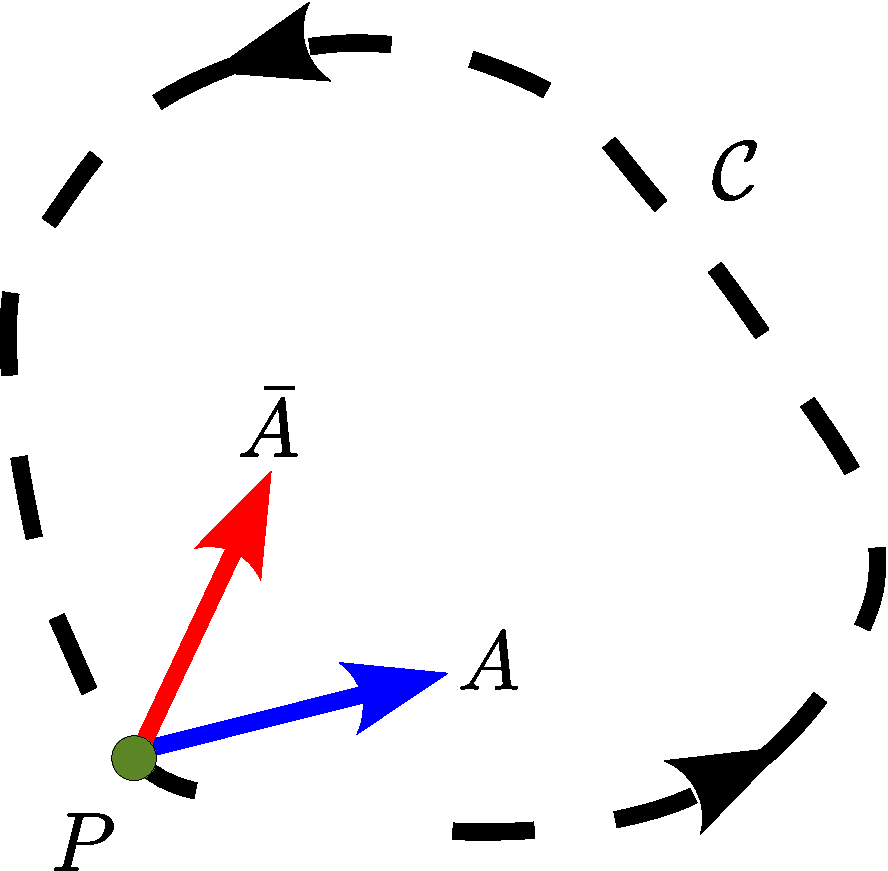
\psfig{file=fig/fig-transporte-curva-cerrada.pdf,height=5cm,angle=0}}
\caption{Transporte paralelo de un vector sobre una curva cerrada.}
\label{dibujo}
\end{figure}
\end{center}
\begin{quotation}
\textbf{Definici'on:} Decimos que una conexi'on $\Gamma$ es \textit{integrable} si y s'olo si el transporte asociado a ella es independiente de la trayectoria.
\end{quotation}
Encontremos las condiciones que debe satisfacer una conexi'on para que sea
integrable.
Para ello, consideremos un vector contravariante $A^i(P)$ asociado a un punto
$P$ de coordenadas $x^i$. Si el transporte es independiente de la trayectoria
usada, entonces puede definirse en forma 'unica un campo vectorial $A^i(x)$ (en todo punto de la variedad) transportando el vector $A^i(P)$ desde $P$ hasta cada punto de la variedad. En este caso podemos expresar el vector en un punto $Q$ infinitesimalmente
pr'oximo a $P$ como
\begin{equation}
A^i(x+dx)=A^i_T(x+dx) . \label{condint}
\end{equation}
Usando $A^i(x+dx)=A^i(x)+(\partial_j A^i)dx^j $ y (\ref{tranAcontr}) obtenemos que
la condici'on (\ref{condint}) es equivalente a
\begin{equation}
\nabla_j A^k=\partial_j A^k+\Gamma_{\ ij}^k A^i =0.
\label{ecdeintegr}%
\end{equation}
\begin{quotation}
\textbf{Resumiendo: si una conexi'on es integrable, existen vectores (no nulos) covariantemente constantes.}
\end{quotation}
Por otro lado, puede considerarse a (\ref{ecdeintegr}) como una ecuaci'on
diferencial que determina el campo (covariantemente constante) $A^i(x)$ dada la conexi'on, suponiendo que 'esta es integrable. Las \textbf{condiciones de
integrabilidad} de esta ecuaci'on son por lo tanto las condiciones para que la
conexi'on sea integrable.


\subsection{No-conmutatividad de las derivadas covariantes, curvatura y torsi'on}\label{sec:RT}
Las segundas derivadas covariantes de un tensor \textit{no conmutan}.
Por ejemplo, usando (\ref{dinv15}) y (\ref{dinv17}) podemos calcular la segunda derivada covariante de un vector arbitrario $A^i$:
\begin{equation}
\nabla_i \nabla_jA^k =\partial_i \partial_jA^{k
}+\partial_i A^l\Gamma_{\ lj}^k +A^l\partial
_i \Gamma_{\ lj}^k +\partial_jA^l\Gamma_{\ li}^k
+A^l\Gamma_{\ lj}^{m}\Gamma_{\ mi}^k -\partial_{l}A^k \Gamma_{\
ji}^l-A^l\Gamma_{\ lm}^k \Gamma_{\ ji}^{m}. \label{segder1}
\end{equation}
A partir de aqu'i, encontramos la siguiente identidad\footnote{Existen identidades similares para cada tipo de tensor. Por ejemplo: $\left[\nabla_i \nabla_j -\nabla_j\nabla_i\right]\phi\equiv T_{\ ij}^{k} \nabla_k\phi$,  $\left[\nabla_i \nabla_j -\nabla_j\nabla_i\right]A_k\equiv -R_{\ kij}^lA_l+T_{\ ij}^{l} \nabla_lA_k$. Es un buen ejercicio demostrar estas identidades ...}
\begin{equation}
\boxed{\nabla_i \nabla_jA^k -\nabla_j\nabla_i A^{k}\equiv R_{\ lij}^k
A^l+T_{\ ij}^{m} \nabla_mA^k ,} \label{cdc}
\end{equation}
donde hemos definido el \textbf{tensor de curvatura} como:
\begin{equation}\marginnote{Curvatura}
\boxed{R_{\ lij}^k :=\partial_i\Gamma_{\ lj}^k -\partial_j\Gamma_{\ li}^k 
+\Gamma_{\ mi}^k \Gamma_{\ lj}^m -\Gamma_{\ mj}^k \Gamma_{\ li}^m .}
\label{curvatura}
\end{equation}
Adem'as, definimos el \textbf{tensor de torsi'on} como:
\begin{equation}\marginnote{Torsi'on}
\boxed{T_{\ ij}^k :=\Gamma_{\ ij}^k -\Gamma_{\ ji}^k .}
\end{equation}

Aunque la curvatura y la torsi'on se definen en t'erminos de la conexi'on,
que no es un tensor, $R_{\ lij}^k$ y $T_{\ ij}^k$ s'i son tensores, como
puede verificarse considerando la consistencia de \eqref{cdc}, o directamente
a partir de su definici'on y la ley de transformaci'on \eqref{dinv72} de la conexi'on.

Note que, como consecuencia directa de su definici'on, estos tensores poseen las siguientes propiedades de antisimetr'ia:
\begin{equation}
R_{\ lij}^k\equiv - R_{\ lji}^k, \qquad T_{\ ij}^k\equiv -T_{\ ji}^k. \label{asRT}
\end{equation}
Estas simetr'ias, reducen el n'umero de componentes linealmente independientes de la curvatura y la torsi'on de \textit{una conexi'on arbitraria} a $n^3(n-1)/2$ y $n^2(n-1)/2$, respectivamente.

Retornando a la identidad \eqref{cdc}, vemos que ella implica que la derivada covariante es independiente del orden de derivaci'on (cuando se aplica a un vector arbitrario) si y s'olo si $R_{\ lji}^k=0$ y $T_{\ ij}^{k}=0$.

Por otro lado, si existe un sistema coordenado donde $\Gamma_{\ ij}^k
\overset{\ast}{=}0$ \textit{en todo punto de una regi'on dada}, entonces la curvatura y la torsi'on ser'an id'enticamente nulas, $R_{\ ijk}^l =0$ y $T_{\ ij}^{k}=0$, en esa regi'on. Adem'as, como la curvatura y la torsi'on son tensores, 'estas se anular'an en todo sistema coordenado.
El contrarec'iproco tambi'en es v'alido. Si existe un sistema
coordenado en el cual la curvatura o la torsi'on sean distintas de cero, $R_{\ ijk}^l \neq 0$ 'o $T_{\ ij}^{k}\neq 0$, entonces no existir'a ning'un sistema coordenado en el cual la conexi'on se anule en la regi'on dada.

Tambi'en es posible probar (aunque es bastante m'as laborioso, y omitiremos la prueba aqu'i. Ver, por ejemplo, la secci'on 6.7 de \cite{Dinverno}) que si la curvatura y la torsi'on de anulan en una regi'on de la variedad entonces es posible encontrar un SC tal que la conexi'on se anule en ese sistema.

En resumen:
\begin{quotation}
\textbf{La condici'on necesaria y suficiente para encontrar un sistema coordenado donde todas las componentes de la conexi'on se anulen en todo punto de una regi'on dada, $\Gamma_{\ ij}^k \overset{\ast}{=}0$, es que $R_{\ ijk}^l=0$ y $T_{\ ij}^k =0$ en esa regi'on.}
\end{quotation}

\subsection{Interpretaci'on geom'etrica de la curvatura*}
\begin{center}
\begin{figure}[h!]
\centerline{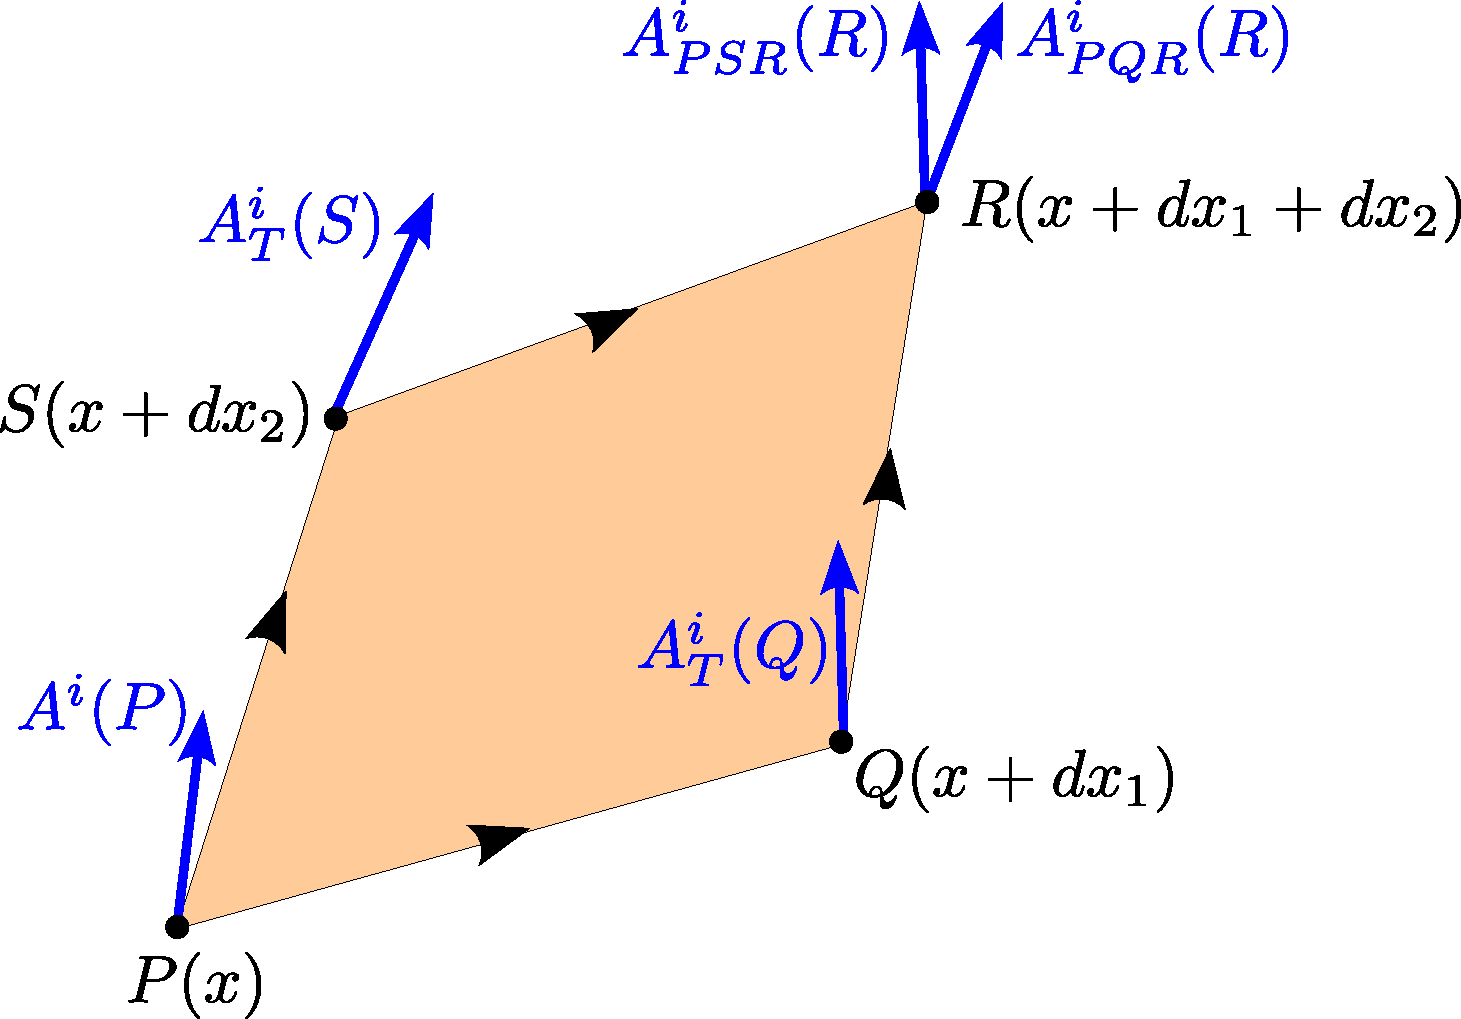
\psfig{file=fig/fig-transporte-y-curvatura-01.pdf,height=6cm,angle=0}}
\caption{Transporte de un vector desde $P$ a $R$ por dos trayectorias (infinitesimales) distintas.}
\label{intgeomcurv}
\end{figure}
\end{center}

Consideremos cuatro puntos $P,Q,R$ y $S$ como en la figura (\ref{intgeomcurv}), con coordenadas $x^i $, $x^i+dx_1^i$, $x^i+dx_1^i+dx_2^i$ y $x^i+dx_2^i$ respectivamente.
Sean $A^i (P)$ las componentes de un vector contravariante definido en el punto $P$. Traslademos este vector a trav'es de la trayectoria $PQR$, obteniendo $\bar{A}^i_{PQR}(R)$, y compar'emoslo con el vector resultante del transporte por la trayectoria $PSR$, $\bar{A}^i_{PSR}(R)$.

Transportamos primero $A^i$ de $P$ a $Q$, obteniendo el vector $A_{T}^i(Q)$:
\begin{equation}
A_{T}^i(Q)=A^i(P) -\Gamma_{\ jk}^i(P)A^j(P)\, dx_1^k .
\label{AT1}%
\end{equation}

Transportamos ahora $A_{T}^i $ desde $Q$ hasta $R$, obteniendo as'i el vector denotado por $A_{PQR}^i (R)$:
\begin{equation}
A_{PQR}^i (R) = A_{T}^i (Q) -\Gamma_{\ jk}^i(Q)A_{T}^j (Q)\,dx_2^k. \label{AT2}%
\end{equation}
 La conexi'on en el lado derecho de (\ref{AT2}) est'a evaluada en el punto $Q$, de coordenadas $x^i +dx_1^i$, y por lo tanto podemos escribir
\begin{equation}
\Gamma_{\ jk}^i(Q)=\Gamma_{\ jk}^i (x+dx_1)=\Gamma_{\ jk}^i(x)+dx_1^l(\partial_l\Gamma_{\ jk}^i) (x) . \label{expGam}
\end{equation}
Reemplazando \eqref{expGam} en \eqref{AT2} y utilizando (\ref{AT1}) obtenemos:%
\begin{align}
A_{PQR}^i (R) &= A^i -\Gamma_{\ jk}^i A^j\,dx_1^k-\Gamma_{\ jk}^i A^j\,dx_2^k \nonumber\\
& \quad  +\Gamma_{\ jk}^i \Gamma_{\ lm}^jA^l\, dx_1^m\,dx_2^k -(\partial_l\Gamma_{\ jk}^i) A^j dx_1^l dx_2^k. \label{AT22}
\end{align}
El c'alculo del vector $A_{\rm PSR}^i(R)$ es an'alogo, con la 'unica diferencia que primero se realiza el desplazamiento coordenado $dx_2^i$ hasta el punto $S$ y luego el desplazamiento en $dx_1^i$ hasta el punto $R$. Por lo tanto, el vector buscado tiene la misma forma que \eqref{AT22}, pero intercambiando $dx_1^i$ con $dx_2^i$, es decir,
\begin{align}
A_{PSR}^i (R) &= A^i -\Gamma_{\ jk}^i A^j\,dx_2^k-\Gamma_{\ jk}^i A^j\,dx_1^k \nonumber\\
& \quad  +\Gamma_{\ jk}^i \Gamma_{\ lm}^jA^l\, dx_2^m\,dx_1^k -(\partial_l\Gamma_{\ jk}^i) A^j dx_2^l dx_1^k. \label{APSR}
\end{align}

%Desplazamos ahora $A_{T2}^i $ desde $R$ hasta $S$, obteniendo $A_{T3}^i (S)$:
%\begin{equation}
%A_{T3}^i (S) = A_{T2}^i(R) -\Gamma_{\ jk}^i(R)A_{T2}^j (R)(-dx_1^k). \label{AT3}%
%\end{equation}
%Aqu'i hemos tomado en cuenta que la diferencia de coordenadas entre los puntos involucrados es $x^i(S)-x^i(R)=-dx_1^k$. Adem'as,
%\begin{equation}
%\Gamma_{\ jk}^i(R)=\Gamma_{\ jk}^i (x+dx_1+dx_2)=\Gamma_{\ jk}^i(x)+(dx_1^l+dx_2^l)(\partial_l\Gamma_{\ jk}^i) (x) . \label{expGam2}
%\end{equation}
%Reemplazando (\ref{expGam2}) en (\ref{AT3}) y utilizando (\ref{AT2}) obtenemos:%
%\begin{equation}
%A_{T3}^i (S) = A^i-\Gamma_{\ jk}^i A^j\,dx_2^k +\left(\partial_k\Gamma_{\ jl}^i-\partial_l\Gamma_{\ jk}^i+\Gamma_{\ mk}^i \Gamma_{\ jl}^m-\Gamma_{\ ml}^i \Gamma_{\ jk}^m\right) A^j\,dx_2^k\,dx_1^l. \label{AT32}
%\end{equation}
%
% Finalmente, trasladamos el vector $A_{T3}^i (S)$ hasta el punto inicial $P$:
%\begin{equation}
%A_{T4}^i(P) = A_{T3}^i(S) -\Gamma_{\ jk}^i(S)A_{T3}^j (S)(-dx_2^k). \label{AT4}%
%\end{equation}
%Usamos $\Gamma_{\ jk}^i(S)=\Gamma_{\ jk}^i(x+dx_2)=\Gamma_{\ jk}^i(x)+dx_2^l(\partial_l\Gamma_{\ jk}^i) (x)$ y nuestro resultado anterior (\ref{AT32}) y finalmente encontramos
%\begin{equation}
%A_{T4}^i(P) =A^i+\left(\partial_k\Gamma_{\ jl}^i-\partial_l\Gamma_{\ jk}^i+\Gamma_{\ mk}^i \Gamma_{\ jl}^m-\Gamma_{\ ml}^i \Gamma_{\ jk}^m\right) A^j\,dx_2^k\,dx_1^l.
%\end{equation}
%Vemos que el segundo t'ermino del lado derecho es precisamente el tensor de curvatura (\ref{curvatura}). As'i obtenemos:
%\begin{equation}
%\boxed{(A_{T4}^i -A^i)(x) =R_{\ jkl}^i(x)\, A^j(x)\,dx_2^k\,dx_1^l.} \label{19}%
%\end{equation}

Comparamos ambos vectores transportado calculando la diferencia de sus componentes. Restando \eqref{AT22} y \eqref{APSR} obtenemos (luego de renombrar algunos 'indices) que el resultado es proporcional al tensor de curvatura \eqref{curvatura},
\begin{equation}
\boxed{(A_{PSR}^i-A^i_{PQR})(R) =R_{\ jkl}^i(x)\, A^j(x)\,dx_1^k\,dx_2^l.} \label{19}%
\end{equation}
%Por lo tanto, la diferencia entre el vector transportado y el original es
%proporcional a la curvatura.
Esto demuestra que el tensor de curvatura de una conexi'on mide localmente (en una regi'on infinitesimal) la magnitud de la dependencia del transporte (inducido por la conexi'on, de vectores y tensores) con la trayectoria.

La relaci'on \eqref{19} que implica que, si la curvatura es nula, el transporte de cualquier vector es independiente de la trayectoria en una regi'on infinitesimal. Este resultado puede extenderse a trayectorias finitas que unan extremos comunes considerando una sucesi'on de ``deformaciones infinitesimales'' de una curva en otra, tal como lo ilustra la figura. Para esto, suponemos que la variedad ``no tiene agujeros'', es decir, que es \textbf{simplemente conexa}. Por lo tanto, si el tensor de curvatura es nulo y la variedad es simplemente conexa entonces el transporte es independiente de la trayectoria, es decir, la conexi'on es integrable.

\subsection{Interpretaci'on geom'etrica de la torsi\'on*}
Consideremos tres puntos $P$, $Q$ y $S$ de la variedad, infinitesimalmente
cercanos, tal que las coordenadas de $P$ son $x^i $, $dx_1^i $ es la
diferencia de las coordenadas entre los puntos $P$ y $Q$, y $dx_2^k $ es la
diferencia de las coordenadas entre los puntos $P$ y $S$ (ver figura \ref{fig:torsion}a). 
Ahora transportamos los vectores contravariantes $dx_1^k $ y $dx_2^k $, ambos definidos en $P$, hasta los puntos $S$ y $Q$, para obtenener as'i $\overline{dx}^i_1$ y $\overline{dx}^i_2$, respectivamente (ver figura \ref{fig:torsion}b). Las componentes de estos nuevos vectores (infinitesimales) est'an dadas entonces por
\begin{center}
\begin{figure}[H]
\centerline{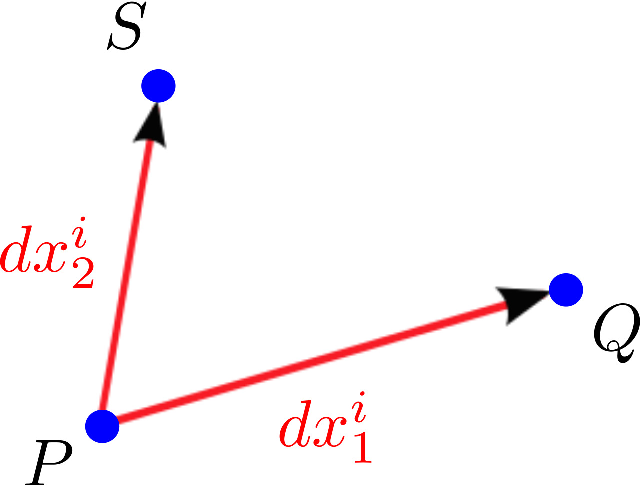
\psfig{file=fig/fig-torsion-01.pdf,height=4cm,angle=0}
\hspace{1cm}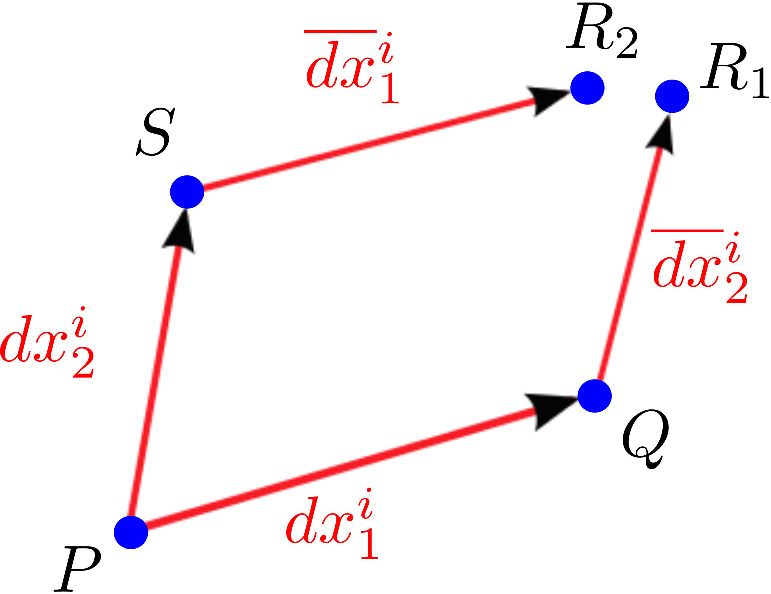
\psfig{file=fig/fig-torsion-02.pdf,height=4cm,angle=0}}
\caption{}
\label{fig:torsion}
\end{figure}
\end{center}
\begin{equation}
\overline{dx}_2^i (Q)=dx_2^i -\Gamma_{\ jk}^i(x)\, dx_2^j dx_1^k ,
\end{equation}
\begin{equation}
\overline{dx}_1^i (S)=dx_2^i -\Gamma_{\ jk}^i(x)\, dx_1^j dx_2^k .
\end{equation}

Los nuevos vectores $\overline{dx}_2^i (Q)$ y $\overline{dx}_1^i (S)$ permiten definir nuevos puntos $R_1$ y $R_2$, cuyas coordenadas son
\begin{equation}
x^i(R_1):=x^i(Q)+\overline{dx}_2^i (Q)=x^i+dx_1^i+dx_2^i -\Gamma_{\ jk}^i(x)\, dx_2^j dx_1^k, 
\end{equation}
\begin{equation}
x^i(R_2):=x^i(S)+\overline{dx}_1^i (S)=x^i +dx_2^i +dx_1^i
 -\Gamma_{\ jk}^i(x)\, dx_1^j dx_2^k .
\end{equation}
En general, los puntos $R_1$ y $R_2$ \textit{no coinciden}: la diferencia entre sus coordenadas est'a dada por
\begin{align}
x^i(R_2)-x^i(R_1) &= -\Gamma_{\ jk}^i(x)\, dx_1^j dx_2^k+ \Gamma_{\ jk}^i(x)\, dx_2^j dx_1^k \\
&=  \left[-\Gamma_{\ jk}^i(x)+ \Gamma_{\ kj}^i(x)\right] dx_1^j dx_2^k \\
&=  -T_{\ jk}^i(x)\, dx_1^j dx_2^k .
\end{align}
Vemos entonces que en la construcci'on geom'etrica discutida de un ``paralel'ogramo infinitesiamal'' los puntos finales no coinciden (el ``paralel'ogramo no se cierra'') si el tensor de torsi'on en no nulo. Debido a esto a menudo se dice que la torsi'on describe (posibles) ``fallas en el cierre local de paralel'ogramos infinitesimales''.



%\subsection{Integrabilidad y curvatura*}
%Vimos en la secci'on \ref{sec:integ} que si una conexi'on es integrable entonces
%existen campos vectoriales no nulos $A^i(x)$ tal que $\nabla_iA^j=0$. Usando esto y la identidad (\ref{cdc}) encontramos el siguiente resultado:
%\begin{quotation}
%\textbf{Teorema:} Si una conexi'on es integrable entonces su tensor de curvatura es nulo.
%\end{quotation}
%Equivalentemente, si el tensor de curvatura de una conexi'on es no nulo, 'esta no es integrable.
%
%Puede tambi'en ser probado que el rec'iproco del teorema anterior es t'ambi'en v'alido. Para esto, usamos \eqref{19} que implica que, si la curvatura es nula, el transporte de cualquier vector es independiente de la trayectoria en una regi'on infinitesimal. Este resultado puede extenderse a trayectorias finitas generales considerando una sucesi'on de ``deformaciones infinitesimales'' de una curva en otra, tal como lo ilustra la figura. Para esto, asumimos que la variedad ``no tiene agujeros'', es decir, que es \textbf{simplemente conexa}.
%
%En resumen:
%\begin{quotation}
%\textbf{Teorema:} Una conexi'on es integrable si y s'olo si su curvatura es
%igual a cero.
%\end{quotation}
% Estas condiciones de integrabilidad pueden obtenerse de la forma usual: las
% segundas derivadas parciales $A^i $ deben conmutar, es decir,
% \begin{equation}
% \frac{\square A^k }{\partial x^m \partial x^j }=\frac{\square %
% A^k }{\partial x^j \partial x^m }. \label{segder}%
% \end{equation}
% De las ecuaciones (\ref{ecdeintegr}) y (\ref{segder}) se obtiene la
% condici'on:
% \begin{equation}
% \frac{\partial}{\partial x^m }\left( \Gamma_{\ ij}^k A^i \right)
% -\frac{\partial}{\partial x^j }\left( \Gamma_{im}^k A^i \right) =0.
% \label{exac}%
% \end{equation}
% Desarrollando obtenemos que%
% \begin{equation}
% A^i \partial_m\Gamma_{\ ij}^k +\Gamma_{\ ij}^k \partial_mA^i %
% -A^i \partial_j\Gamma_{im}^k -\Gamma_{im}^k \partial_jA^i =0.
% \label{10}%
% \end{equation}
% Reemplazando $\partial_jA^k $ en (\ref{10}) tenemos:%
% \begin{align}
% A^i \partial_m\Gamma_{\ ij}^k -A^i \partial_j\Gamma_{im}^k +\Gamma
% _{lm}^k \Gamma_{\ ij}^l A^i -\Gamma_{lj}^k \Gamma_{im}^l A^i  & =0,\\
% A^i \left( \partial_m\Gamma_{\ ij}^k -\partial_j\Gamma_{im}^k %
% +\Gamma_{lm}^k \Gamma_{\ ij}^l -\Gamma_{lj}^k \Gamma_{im}^l \right)  & =0.
% \label{12}%
% \end{align}
% Como $A^i $ es un vector arbitrario, la condici'on de integrabilidad es:%
% \begin{equation}
% \partial_m\Gamma_{\ ij}^k -\partial_j\Gamma_{im}^k +\Gamma_{lm}^k %
% \Gamma_{\ ij}^l -\Gamma_{lj}^k \Gamma_{im}^l =0.
% \end{equation}


Por ejemplo, en el caso de un plano ($E_2$) sabemos que el transporte es independiente de la trayectoria, y por lo tanto la conexi'on es integrable. Adem'as, en coordenadas cartesianas\footnote{Utilizamos el s'imbolo $\overset{\ast}{=}$ para denotar que esta igualdad es v'alida s'olo en un sistema coordenado particular.} $\Gamma_{\ ij}^k \overset{\ast}{=}0$. En este caso,
seg'un (\ref{curvatura}), tenemos que la curvatura se anula, $R_{\ ijk}^l =0$.

%\subsection{Condiciones de Integrabilidad}\label{sec-ci}
%Puesto que el an'alisis realizado es s'olo fruto de reescribir la
%ecuaci'on del movimiento de una part{\'\i}cula libre en un SR
%no-inercial, debe entonces ser posible, dados $\bar{\Gamma }$ y/o
%$\bar{g}$ en alg'un SR, retornar a un SRI con sus coordenas inerciales asociadas. En
%este caso (compare (\ref{tsri}) y (\ref{tsrni})) la conexi'on $\Gamma$ se anula
%id'enticamente y la m'etrica adopta su forma minkowskiana. En otras palabras, un SRI queda determinado por los requerimientos que $g_{\mu\nu }=\eta _{\mu\nu }$ y $%
%\Gamma _{\ \mu\nu }^\lambda =0$ \emph{globalmente}, es decir, en todo punto del
%espaciotiempo.
%
%Estudiaremos ahora las condiciones que las componentes de una conexi'on
%$\bar{\Gamma }$ en un sistema coordenado $\bar x$ deben satisfacer de modo que
%exista la transformaci'on $\bar{x}\to x$ de vuelta a un SRI.
%
%De la ley de transformaci'on (\ref{tigam}) vemos que la condici'on para que en
%el nuevo sistema de coordenadas $\Gamma=0$ es
%\begin{equation}
%\frac{\partial x^\mu}{\partial \bar{x}^\sigma }\frac{\partial \bar{x}^\rho
%}{\partial x^{\nu }}\frac{\partial\bar{x}^{\eta }}{\partial
%x^\lambda}\bar{\Gamma }_{\ \rho \eta}^\sigma (\bar{x})+\frac{\partial x^{\mu
%}}{\partial \bar{x}^\rho }\frac{\partial ^2\bar{x}^\rho }{\partial
%x^{\nu}\partial x^\lambda }=0.
%\end{equation}
%De aqu'i, obtenemos
%\begin{equation}
%\frac{\partial ^2\bar{x}^\alpha }{\partial x^{\nu }\partial
%x^\lambda }=-\frac{\partial \bar{x}^\rho }{\partial x^{\nu }}%
%\frac{\partial \bar{x}^{\eta }}{\partial x^\lambda }\bar{%
%\Gamma }_{\ \rho \eta }^\alpha (\bar{x}) .\label{2der}
%\end{equation}
%
%Ya que, asumiendo que la transformaci'on $\bar{x}\to x$ existe, el lado
%izquierdo de (\ref{2der}) es sim'etrico bajo intercambio de los 'indices $\nu$
%y $\lambda$, debe cumplirse que el lado derecho tambi'en lo sea. Esta
%condici'on es equivalente a
%\begin{equation}
%\boxed{\bar{\Gamma }_{\ \mu\nu}^\lambda
%=\bar{\Gamma}_{\ \nu\mu}^\lambda.}
%\end{equation}
%
%Otra condici'on puede ser encontrada usando el hecho que el lado derecho de
%(\ref{2der}) debe efectivamente ser igual a las segundas derivadas de las
%funciones que definen el cambio de coordenadas. Para esto, derivamos
%(\ref{2der}) nuevamente y obtenemos:
%\begin{eqnarray}
%\frac{\partial ^3\bar{x}^\alpha }{\partial x^\rho \partial
%x^{\nu }\partial x^\lambda } &=&-\frac{\partial }{\partial x^\rho }\left(
%\frac{\partial \bar{x}^\beta }{\partial x^{\nu }}\frac{\partial
%\bar{x}^{\gamma }}{\partial x^\lambda }\bar{\Gamma }_{\ \beta
%\gamma }^\alpha \right) \\
%\frac{\partial ^3\bar{x}^\alpha }{\partial x^\rho \partial
%x^{\nu }\partial x^\lambda } &=&-\left[ \frac{\partial ^2\bar{x}%
%^\beta }{\partial x^\rho \partial x^{\nu }}\frac{\partial \bar{x}%
%^{\gamma }}{\partial x^\lambda }\bar{\Gamma }_{\ \beta \gamma
%}^\alpha +\frac{\partial \bar{x}^\beta }{\partial x^{\nu }}%
%\frac{\partial ^2\bar{x}^{\gamma }}{\partial x^\lambda \partial
%x^\rho }\bar{\Gamma }_{\ \beta \gamma }^\alpha +\frac{\partial
%\bar{x}^\beta }{\partial x^{\nu }}\frac{\partial \bar{x}%
%^{\gamma }}{\partial x^\lambda }\frac{\partial \bar{x}^{\delta }}{%
%\partial x^\rho }\frac{\partial \bar{\Gamma }_{\ \beta \gamma
%}^\alpha }{\partial \bar{x}^{\delta}}\right].
%\end{eqnarray}%
%Reemplazando, las segundas derivadas usando (\ref{2der}) nuevamente, llegamos
%a
%\begin{eqnarray}
%\frac{\partial ^3\bar{x}^\alpha }{\partial x^\rho \partial
%x^{\nu }\partial x^\lambda }&=&\frac{\partial \bar{x}^\sigma }{%
%\partial x^\rho }\frac{\partial \bar{x}^{\eta }}{\partial x^{\nu }}%
%\bar{\Gamma }_{\ \sigma \eta }^\beta \frac{\partial \bar{x}%
%^{\gamma }}{\partial x^\lambda }\bar{\Gamma }_{\ \beta \gamma
%}^\alpha +\frac{\partial \bar{x}^\beta }{\partial x^{\nu }}%
%\frac{\partial \bar{x}^\sigma }{\partial x^\lambda }\frac{\partial
%\bar{x}^{\eta }}{\partial x^\rho }\bar{\Gamma }_{\ \sigma \eta
%}^{\gamma }\bar{\Gamma }_{\ \beta \gamma }^\alpha -\frac{\partial
%\bar{x}^\beta }{\partial x^{\nu }}\frac{\partial \bar{x}%
%^{\gamma }}{\partial x^\lambda }\frac{\partial \bar{x}^{\delta }}{%
%\partial x^\rho }\frac{\partial \bar{\Gamma }_{\ \beta \gamma
%}^\alpha }{\partial \bar{x}^{\delta }} \\
%&=&-\frac{\partial \bar{x}^\beta }{\partial x^{\nu }}\frac{%
%\partial \bar{x}^{\gamma }}{\partial x^\lambda }\frac{\partial
%\bar{x}^{\delta }}{\partial x^\rho }\left( \frac{\partial \bar{%
%\Gamma }_{\ \beta \gamma }^\alpha }{\partial \bar{x}^{\delta }}
%-\bar{\Gamma }_{\sigma\gamma }^\alpha \bar{\Gamma }_{\ \delta \beta
%}^\sigma -\bar{\Gamma }_{\ \beta \sigma }^\alpha \bar{\Gamma }_{\ \gamma
%\delta }^\sigma \right).
%\end{eqnarray}
%Nuevamente, ya que el lado izquierdo de esta expresi'on debe ser sim'etrico
%bajo intercambio de los 'indices $\lambda$ y $\rho$, es decir,
%\begin{equation}
%\frac{\partial ^3\bar{x}^\alpha }{\partial x^\rho \partial
%x^{\nu }\partial x^\lambda }\equiv\frac{\partial ^3\bar{x}^\alpha }{\partial
%x^\lambda \partial x^{\nu }\partial x^\rho },
%\end{equation}
%obtenemos la siguiente condici'on para las componentes de $\bar\Gamma$ y sus
%derivadas:
%\begin{equation}
%\frac{\partial \bar{\Gamma }_{\ \beta \gamma }^{\alpha
%}}{\partial \bar{x}^{\delta }}-\bar{\Gamma }_{\ \sigma \gamma
%}^\alpha \bar{\Gamma }_{\ \delta \beta }^\sigma -\bar{\Gamma }_{\ \beta
%\sigma }^\alpha \bar{\Gamma }_{\ \gamma \delta }^\sigma =\frac{\partial
%\bar{\Gamma }_{\ \beta \delta }^\alpha }{\partial \bar{x}^{\gamma
%}}-\bar{\Gamma }_{\ \sigma\delta}^\alpha\bar{\Gamma}_{\ \gamma\beta}^\sigma -\bar{\Gamma }_{\ \beta\sigma }^\alpha \bar{\Gamma }_{\ \delta
%\gamma }^\sigma .
%\end{equation}
%Definiendo (el tensor de curvatura, ver secci'on \ref{sec:intcurv})
%\begin{equation}
%\boxed{\bar{R}_{\ \mu\nu\lambda }^\rho :=\frac{\partial
%\bar{\Gamma }_{\ \mu\lambda }^\rho }{\partial \bar{x}^{\nu
%}}-\frac{\partial \bar{\Gamma }_{\ \mu\nu }^\rho }{\partial
%\bar{x}^{\lambda }}+\bar{\Gamma }_{\ \sigma \nu}^{\rho}\bar{\Gamma}_{\ \mu\lambda }^\sigma-\bar{\Gamma}_{\ \sigma \lambda}^{\rho}\bar{\Gamma}_{\ \mu\nu }^\sigma,}
%\end{equation}
%podemos escribir la segunda condici'on de integrabilidad simplemente como:
%\begin{equation}
%\boxed{\bar{R}_{\ \mu\nu\lambda }^\rho =0.}
%\end{equation}
%Note que el tensor de curvatura es antisim'etrico en sus dos 'ultimos 'indices:
%\begin{equation}
%\bar{R}_{\ \mu\nu\lambda}^\rho\equiv -\bar{R}_{\ \mu\lambda\nu}^\rho.
%\end{equation}
%
%Este tensor de curvatura puede ser calculado en cualquier SC, por ejemplo, en coordenadas $\tilde{x}$, tendremos
%\begin{equation}
%\tilde{R}_{\ \mu\nu\lambda }^\rho =\frac{\partial
%\tilde{\Gamma }_{\ \mu\lambda }^\rho }{\partial \tilde{x}^{\nu
%}}-\frac{\partial \tilde{\Gamma }_{\ \mu\nu }^\rho }{\partial
%\tilde{x}^{\lambda }}+\tilde{\Gamma }_{\ \sigma \nu}^{\rho}\tilde{\Gamma}_{\ \mu\lambda }^\sigma-\tilde{\Gamma}_{\ \sigma \lambda}^{\rho}\tilde{\Gamma}_{\ \mu\nu }^\sigma,
%\end{equation}
%que determinan entonces las condiciones de integrabilidad para la conexi'on $\tilde{\Gamma}$ en ese SC. Usando el hecho que lsa componentes $\tilde{\Gamma}$ y $\bar{\Gamma}$ est'an relacionadas por medio de (\ref{tigam}), es posible verificar que la relaci'on entre las componentes de $\tilde{R}$ y $\bar{R}$ es
%\begin{equation}
% \tilde{R}_{\ \mu\nu\lambda }^\rho =\frac{\partial \tilde{x}^\rho}{\partial \bar{x}^{\alpha}}\frac{\partial\bar{x}^{\beta}}{\partial \tilde{x}^\mu}\frac{\partial\bar{x}^{\gamma}}{\partial \tilde{x}^\nu}\frac{\partial\bar{x}^{\delta}}{\partial\tilde{x}^\lambda}\,\bar{R}_{\ \beta\gamma\delta}^\alpha . \label{ltR}
%\end{equation}
%Esta ley de transformaci'on justifica, como discutiremos en el pr'oximo cap'itulo, considerar que $\tilde{R}_{\ \mu\nu\lambda }^\rho$ y $\bar{R}_{\ \beta\gamma\delta}^\alpha$ con componentes en distintos SC's de un \textit{tensor}, el tensor de curvatura de Riemann.
%
%En resumen, hemos encontrado que la condici'on de integrabilidad de una conexi'on, es decir, la condici'on necesaria para que sus componentes puedan ser anuladas al realizar una transformaci'on de coordenadas, es que 'esta sea sim'etrica en sus 'indices inferiores (condici'on de torsi'on nula) y que su tensor de curvatura asociado sea nulo. Adem'as, la ley de transformaci'on (\ref{ltR}) asegura que si la condici'on de integrabilidad es satisfecha por las componentes de la conexi'on en un SC, entonces ser'a satisfecha \textit{en todo SC}. Note finalmente que en el caso que hemos analizado, que es simplemente la teor'ia de RE formulada en SC's asociados a SR no-inerciales, las condiciones de integrabilidad de la conexi'on son naturalmente satisfechas.
%
%Como discutiremos con mayor detalle y precisi'on en el cap'itulo \ref{capTEG}, la teor'ia de gravitaci'on de Einstein, la teor'ia General de la Relatividad, se basa en la idea que los efectos de un campo gravitacional homog'eneo son equivalentes a aquellos observados en sistemas de referencia acelerados, y por lo tanto pueden ser ``anulados'' en todo punto eligiendo convenientemente el SR, pero que campos no-homog'eneos (campos gravitacionales ``no-triviales'', como el producido por la Tierra, por ejemplo) no pueden ser anulados globalmente. Esto se describe matem'aticamente usando conexiones que \textit{no satisfacen la condici'on de integrabilidad}, es decir, que tienen un tensor de curvatura no nulo.

\subsection{Curvas autoparalelas*}
% \begin{center}
% \begin{figure}[H]
% \centerline{\psfig{file=4.ps,height=3cm,angle=0}}
% \caption{}
% \label{autoparalelas}
% \end{figure}
% \end{center}
Se dice que una curva es \textbf{autoparalela} si satisface que sus vectores tangentes son paralelos (respecto al transporte definido por una conex'on $\Gamma$) a lo largo de la misma curva. En otras palabras, si $x^i(\lambda)$ es la parametrizaci'on de la curva, entonces ella es autoparalela si su vector tangente $u^i(\lambda):=dx^i/d\lambda$ evaluado en el punto correspondiente a $\lambda+d\lambda$ (es decir, el punto con coordenadas $x^i(\lambda+d\lambda)$) es \textit{proporcional} al vector resultante de transportar $u^i(\lambda)$ (definido el punto correspondiente al par'ametro $\lambda$, es decir, con coordenadas $x^i(\lambda)$) hasta el punto con par'ametro $\lambda+d\lambda$. Es usual describir a las curvas autoparalelas como ``las m'as rectas posibles'' en el sentido que ellas siguen la direcci'on de sus propios vectores tangentes, transportados de punto a punto por medio de la conexi'on.


Es simple verificar que una curva autoparalela debe satisfacer una ecuaci'on de la forma
\begin{equation}\marginnote{ec. curvas autoparalelas}
\boxed{\frac{d^2x^i}{d\lambda^2}+\Gamma_{jk}^i \frac{dx^j}{d\lambda}
\frac{dx^k}{d\lambda} =f(\lambda)\frac{dx^i}{d\lambda}.}
\end{equation}
Tal como en el caso de las curvas de longitud extrema (geod'esicas), es posible elegir un par'ametro af'in tal que $f=0$. 
%
% Bajo un cambio de par'ametro $s=s(\lambda)$,\ la ecuaci'on (\ref{s4}) se
% transforma en:%
% \begin{equation}
% \frac{d^2x^k }{ds^2}+\Gamma_{lm}^k \frac{dx^l }{ds}\frac{dx^m }%
% {ds}=\frac{\phi s'-s^{\prime\prime}}{s^{\prime2}}\frac{dx^k }%
% {ds}, \label{s5}%
% \end{equation}
% donde $s':=ds/d\lambda$. El segundo miembro de esta ecuaci'on se
% anula si y s'olo si $\phi s'-s^{\prime\prime}=0$, es decir, si:%
% \begin{equation}
% s=\int^{\lambda}\exp\left[ \int^{\lambda'}\phi(u)du\right]
% d\lambda'. \label{s6}%
% \end{equation}
% De este modo, siempre es posible escoger un par'ametro tal que el segundo
% miembro de (\ref{s6}) se anule. En este caso, el par'ametro $s$ es llamado
% \textit{par'ametro af'in} y la ecuaci'on para la curva autoparalela se reduce
% a
% \begin{equation}
% \boxed{\frac{d^2x^k }{ds^2}+\Gamma_{\ lm}^k \frac{dx^l }{ds}\frac{dx^m }%
% {ds}=0.} \label{s7}%
% \end{equation}
% Se verifica directamente que esta ecuaci'on mantiene su forma bajo cualquier
% transformaci'on lineal del par'ametro af'in ($\hat{s}=as+b,$ con $a$, $b$
% constantes). De este modo, las soluciones de la ecuaci'on (\ref{s7}),
% $x^i =x^i (s)$, son representaciones param'etricas de las curvas autoparalelas
% asociadas a una conexi'on $\Gamma$.

\section{Geometr'ia riemanniana}

La \textbf{geometr'ia riemanniana}\footnote{Llamada as'i en honor de Bernhard Riemann: 1826-1866, matem'atico alem'an. Ver \url{http://es.wikipedia.org/wiki/Bernhard_Riemann}.} es una generalizaci'on de la geometr'ia intr'inseca de las superficies gaussianas (originalmente, superficies inmersas en $E_3$), a espacios de dimensiones superiores. En una geometr'ia riemanniana tanto las propiedades m'etricas (longitudes, 'areas, vol'umenes, m'odulos de vectores, geod'esicas, etc) como las propiedades afines (derivadas covariantes, transporte, curvatura, torsi'on, curvas autoparalelas) quedan determinadas por un 'unico objeto: la m'etrica. En particular en una geometr'ia de Riemann, la conexi'on es aquella determinada por los s'imbolos de Christoffel asociados al tensor m'etrico, adicionalmente el tensor de torsi'on se anula id'enticamente, pero el tensor de curvatura es en general no nulo. Adem'as, en una geometr'ia riemanninana las curvas autoparalelas coinciden con las geod'esicas.



\subsection{Propiedades de los s'imbolos de Christoffel}

Los s'imbolos de Christoffel (\ref{gm6}) definen una conexi'on que posee torsi'on id'enticamente nula (pues es sim'etrica bajo permutaci'on de sus 'indices covariantes), pero que tiene en general curvatura no nula: $R^i_{\ jkl}(\left\{_{ \ }^{\ }\right\})\neq 0$, $T^i_{\ jk}(\left\{_{ \ }^{\ }\right\})\equiv 0$.

Es 'util notar que, usando esta conexi'on, la ecuaci'on de la geod'esica (\ref{gm5}) puede escribirse
como
\begin{equation}
 v^j\nabla_jv^i=fv^i, \label{egdc}
\end{equation}
donde $v^i:={dx^i}/{d\lambda}$ representan los vectores tangentes sobre la
curva.

Adem'as, puede verificarse directamente que la derivada covariante definida por
la conexi'on (\ref{gm6}) satisface la \textbf{condici'on de metricidad}
\begin{equation}\marginnote{Condici'on de metricidad}
\boxed{\nabla_kg_{ij}\equiv 0,} \label{tI1}%
\end{equation}
o, equivalentemente,
\begin{equation}
\nabla_kg^{ij}\equiv 0. \label{tIi2}%
\end{equation}

[* Esta propiedad puede interpretarse geom'etricamente como la condici'on que
asegura que el m'odulo de un vector arbitrario permanezca inalterado al ser
transportado.]

M'as a'un, puede probarse que la 'unica conexi'on que satisface i) que su
torsi'on sea id'enticamente nula y ii) que satisfaga la condici'on de metricidad
(\ref{tI1}) es precisamente la conexi'on (\ref{gm6}).

% \subsubsection{Condici'on de metricidad}
%
% Para empezar vamos a demostrar dos importantes teoremas.
%
% \begin{quotation}
% \textbf{Teorema:} Sea $M_n$ una variedad con una m'etrica $g_{ij}$ y una
% conexi'on $\Gamma_{\ i j}^{k}$. Entonces, la longitud de un vector bajo
% transporte paralelo es conservada si y s'olo si:
% \begin{equation}
% \nabla_kg_{ij}=0. \label{tI1}%
% \end{equation}
% \end{quotation}
% En efecto, sea $A^i (x)$ un vector definido en $P$ (con coordenadas $x^i$), y
% $A_T^i (x+dx)$ el vector que resulta de transportar $A^i $ desde $P$ hasta
% $Q$ (con coordenadas $x^i+dx^i$), es decir,
% \begin{equation}
% A_T^i (Q)=\left( A^i -\Gamma_{\ l m}^i A^{ l}%
% dx^{ m}\right) _{P}. \label{tI2}%
% \end{equation}
% Las longitudes de $A^i $ y $A_T^i $ son, respectivamente:%
% \begin{equation}
% \left\vert A\right\vert ^2=\left( g_{ij}A^i A^j \right) _{P},
% \label{tI3}%
% \end{equation}
% \begin{equation}
% \left\vert A_T\right\vert ^2=\left( g_{ij}A_T^i A_T%
% ^j \right) _{Q}. \label{tI4}%
% \end{equation}
% Pero
% \begin{equation}
% g_{ij}(Q)=\left( g_{ij}+\partial_{ l}g_{ij}dx^l\right) _{P}, \label{tI5}%
% \end{equation}
% por lo tanto:
% \begin{equation}
% \left\vert A_T\right\vert ^2=\left[ g_{ij}+\partial_{ l}%
% g_{ij}dx^{ l}\right] \left[ A^i -\Gamma_{\ l m}^{ i
% }A^{ l}dx^{ m}\right] \left[ A^j -\Gamma_{\ l m}^{ j
% }A^{ l}dx^{ m}\right] . \label{tI6}%
% \end{equation}
% Desarrollando el producto a primer orden en $dx^{ l}$, encontramos:
% \begin{equation}
% \left\vert A_T\right\vert ^2=g_{ij}A^i A^j -g_{ij}%
% \Gamma_{\ kl}^j A^i A^{k}dx^l-g_{ij}%
% \Gamma_{\ lm}^i A^{ l}A^j dx^{ m}+(\partial_kg_{ij}) A^i A^j dx^k.
% \label{tI7}%
% \end{equation}
% Igualando (\ref{tI3}) y (\ref{tI7}) se obtiene la condici'on
% \begin{equation}
% -g_{ij}\Gamma_{\ kl}^j A^i A^kdx^l-g_{ij}\Gamma_{\ lm}^i A^{ l}A^j
% dx^m+(\partial_kg_{ij}) A^i A^j dx^k=0. \label{tI8}%
% \end{equation}
% Intercambiando adecuadamente los 'indices mudos se obtiene:%
% \begin{equation}
% \left(\partial_kg_{ij}-g_{il}\Gamma_{\ jk}^l-g_{lj}\Gamma_{\ ik}^l\right)
% A^i A^j dx^k =0.
% \end{equation}
% Usando la arbitrariedad de $A^i $ y $dx^i $ obtenemos:
% \begin{equation}
% \partial_kg_{ij}-g_{il}\Gamma_{\ jk}^ll-g_{lj}\Gamma_{\ ik}^l=0 ,\label{tI10}
% \end{equation}
% es decir, que la derivada covariante de la m'etrica debe anularse.

% \subsection{Condici'ones de metricidad, torsi'on y s'imbolos de Christoffel}
%
% \begin{quotation}
% \textbf{Teorema:} La 'unica conexi'on que satisface:
% \begin{enumerate}
% \item $T_{ij}^{k}=0$ (torsi'on nula o, equivalentemente, $\Gamma$
% sim'etrico en sus 'indices covariantes),
% \item $\nabla_kg_{ij}=0$ (condici'on de metricidad: la longitud de
% un vector no cambia bajo transporte paralelo),
% \end{enumerate}
% es el s'imbolo de Christoffel (\ref{gm6}).
% \end{quotation}
% En efecto, de la condici'on de metricidad tenemos:
% \begin{equation}
% \nabla_kg_{ij}=\partial_kg_{ij}-g_{il}\Gamma_{\ j k}^l-g_{lj}\Gamma_{\ i
% k}^l=0. \label{tII2}%
% \end{equation}
% Luego:
% \begin{equation}
% \partial_kg_{ij}=g_{l j}\Gamma_{\ i k}^l+g_{ il}\Gamma_{\ j k}^l.
% \label{tII3}%
% \end{equation}
% Escribamos las ecuaciones que se obtienen por permutaci'on circular de los
% 'indices $ k$, $ i$, $ j$:%
% \begin{equation}
% \partial_i g_{ j k}=g_{l k}\Gamma_{\ j i}^l+g_{ jl
% }\Gamma_{\ k i}^l ,\label{tII4}%
% \end{equation}%
% \begin{equation}
% \partial_j g_{k i}=g_{l i}\Gamma_{\ k i}^l%
% +g_{kl}\Gamma_{\ ij}^l. \label{tII5}%
% \end{equation}
% Sumando (\ref{tII3}) a (\ref{tII4}) y restando (\ref{tII5}) se obtiene:%
% \begin{equation}
% \partial_kg_{ij}+\partial_i g_{ j k}-\partial_{ j
% }g_{k i}=g_{l j}\left( \Gamma_{\ i k}^l+\Gamma_{\ k i}^l\right) +g_{
% il}\left( \Gamma_{\ j k}^l-\Gamma_{\ k i}^l\right) +g_{l k}\left(
% \Gamma_{\% ji}^l-\Gamma_{\ ij}^l\right) . \label{tII6}%
% \end{equation}
% Usando la condici'on de torsi'on nula la ecuaci'on (\ref{tII6}) se reduce a
% \begin{equation}
% \partial_kg_{ij}+\partial_i g_{ j k}-\partial_{ j
% }g_{k i}=2g_{l j}\Gamma_{\ i k}^l, \label{tII7}%
% \end{equation}%
% es decir,
% \begin{equation}
% g_{l j}\Gamma_{\ i k}^l=\frac{1}2\left[ \partial_{k
% }g_{ij}+\partial_i g_{ j k}-\partial_j g_{k i}\right]
% =:\left\{  j i k\right\} . \label{tII8}%
% \end{equation}
% Los s'imbolos $\left\{  j i k\right\} $ se denominan \textit{s'imbolos
% de Christoffel de primera especie}. Multiplicando por $g^{ j m}$,
% obtenemos:%
% \begin{align}
% \delta_{l}^{ m}\Gamma_{\ i k}^l & =\frac{1}2g^{ j m
% }\left[ \partial_kg_{ij}+\partial_i g_{ j k}%
% -\partial_j g_{k i}\right] ,\label{tII9}\\
% \Gamma_{\ i k}^{ m} & =\frac{1}2g^{ j m}\left[ \partial
% _kg_{ij}+\partial_i g_{ j k}-\partial_j g_{k i
% }\right] \equiv\left\{ _{ i k}^{ m}\right\} .
% \end{align}

\begin{quotation}
\textbf{\textit{Desde ahora en adelante consideraremos siempre geometr'ias riemannianas, es
decir, donde la conexi'on es dada por los s'imbolos de Christoffel.}}
\end{quotation}

\subsection{Espacios planos}
Se dice que un espacio con geometr'ia riemanniana es \textbf{plano} si y s'olo si existen sistemas de coordenadas en los que las componentes del tensor m'etrico sean \textit{constantes} (es decir, independientes de las coordenadas). Como consecuencia tenemos que:
\begin{quotation}
\textbf{Si un espacio riemanniano es plano entonces su tensor de curvatura de Riemann es nulo.}
\end{quotation}
En efecto, $g_{ij}\overset{\ast}{=}$ cte. implica $\{ _{ i j}^{\, k}\}
\overset{\ast}{=}0$ y por tanto $R_{\ i j k}^l=0$. Ejemplos de estos
espacios son el espacio de Minkowski de la teor'ia de Relatividad Especial y
los espacios euclideanos\footnote{Note que un cil'indro es tambi'en un espacio plano.}.

Por supuesto, el contrarrec'iproco es tambi'en verdadero:
\begin{quotation}
\textbf{Si $R_{\ ijk}^l\neq0$
entonces \textit{no existe} un sistema coordenado donde $g_{ij}\overset{\ast}{=}{\rm
cte.}$ y $\{ _{ i j}^{\, k}\} \overset{\ast}{=}0$ \textit{en todo punto}}.
\end{quotation}

An'alogamente, es posible probar el resultado rec'iproco: si el tensor de curvatura de Riemann se anula en todo punto entonces es posible encontrar un SC en el que la m'etrica asuma valores constantes. Para esto, basta aplicar el resultado visto al final de la secci'on (\ref{sec:RT}) y la identidad $\partial_kg_{ij}\equiv g_{il}\,\{ ^{\, l} _{jk}\}+g_{jl}\,\{ ^{\, l} _{ik}\}$, que es equivalente a (\ref{tI1}).

En resumen:
\begin{quotation}
\textbf{La condici'on necesaria y suficiente para que existan sistemas coordenados en los que la m'etrica sea constante es que su tensor de curvatura de Riemann sea nulo.}
\end{quotation}
% \subsection{S'imbolo de Christoffel contraido}
%
% De (\ref{gm6}) obtenemos que la contracci'on $\Gamma_{\ j i}^i$ es dada por:
% \begin{eqnarray}
% \Gamma_{\ j i}^i &=&\frac{1}2g^{ ik}\left( \partial_ig_k+\partial_j
% g_{k i}-\partial_k g_{ji}\right)\\
% &=&\frac{1}{2}g^{ ik}\partial_j g_{ki}
% \end{eqnarray}
% Usando ahora la identidad\footnote{No presentaremos aqu'i una demostraci'on
% general de esta identidad, v'alida en cualquier dimensi'on, para cualquier
% m'etrica invertible. El lector puede verificar su validez explicitamente en
% los casos bi- y tri-dimensional.}
% \begin{equation}
% \partial_k g\equiv gg^{ij}\partial_k g_{ij},
% \end{equation}
% podemos escribir
% \begin{equation}
% \Gamma_{\ ji}^i =\frac{1}{2}g^{ ik}\partial_j
% g_{ki}=\frac{1}{2g}\partial_j g=\partial_j \ln\sqrt{\left\vert g\right\vert}.
% \end{equation}
% Por lo tanto,
% \begin{equation}
% \boxed{\Gamma_{\ j i}^i =\partial_j \ln\sqrt{\left\vert g\right\vert }.}
% \end{equation}

% Se puede demostrar que la conexi'on de Cristoffel satisface
% \begin{equation}
% \Gamma_{ i k}^i =\frac{1}{\sqrt{\left| g\right| }}\partial
% _k\sqrt{\left| g\right| }%
% \end{equation}
% y esto implica que
% \begin{equation}
% \nabla_i V^i =\frac{1}{\sqrt{\left| g\right| }}\partial_i \left(
% \sqrt{\left| g\right| }V^i \right)
% \end{equation}
%
% Es directo verificar que la derivada covariante de la m'etrica con respecto
% a la conexi'on m'etrica (s'imbolo de Christoffel) es
% id'enticamente nula. Para la inversa tambi'en se tiene $\nabla_{k
% }g^{ij}=0$.


\subsection{Coordenadas geod'esicas}\label{secCG}

Puede mostrarse que, cuando la curvatura es no nula, si bien no es posible encontrar un SC en el cual la m'etrica sea constante y la conexi'on se anule \textit{en todo punto} de una regi'on dada, s'i es posible encontrar un SC tal que \textit{en un punto dado} $P$ de la variedad, se satisfaga
\begin{equation}
 g_{ij}(P)\overset{\ast}{=}diag(\pm 1,\cdots,\pm 1)=:\eta_{ij}, \qquad \left\{_{ij}^{\,
k}\right\}(P) \overset{\ast}{=}0,
\end{equation}
o, equivalentemente
\begin{equation}
 g_{ij}(P)\overset{\ast}{=}\eta_{ij}, \qquad \partial_k
g_{ij}(P) \overset{\ast}{=}0. \label{cg1}
\end{equation}
Estas coordenadas reciben el nombre de \textbf{coordenadas geod'esicas}.
Note que, sin embargo, necesariamente $\partial_l\partial_k g_{ij}(P)\overset{\ast}{\neq}0$, ya que $R_{\
ijk}^l(P)\neq0$ requiere que $\partial_l\left\{
_{ik}^{\,m}\right\}(P)\overset{\ast}{\neq}0$.

Una forma de entender el rol de las coordenadas geod'esicas es expresando la m'etrica en una vecindad del punto $P$ en t'erminos de una serie de potencias en torno a $P$. Denotando las coordenadas de $P$ como $x^i$ podemos, en cualquier SC, escribir:
\begin{equation}
 g_{ij}(x+\Delta x)=g_{ij}(P)+\Delta x^k(\partial_kg_{ij})(P)+\frac{1}{2}\Delta x^k\Delta x^l(\partial_k\partial_lg_{ij})(P)+\cdots . \label{expg}
\end{equation}
En un espacio plano, es posible encontrar coordenadas en las que la m'etrica es constante, es decir, asume el mismo valor \textit{en todo punto}, entonces todas las derivadas $\partial_kg_{ij}(P)\stackrel{*}{=}0$, $\partial_k\partial_lg_{ij}(P)\stackrel{*}{=}0$, etc. se anulan y la expansi'on anterior (\ref{expg}) se reduce a s'olo el primer t'ermino, de la forma est'andar $\eta_{ij}$.

Por otro lado, en un espacio curvo ``s'olo'' es posible encontrar coordenadas geod'esicas en las que se satisfaga (\ref{cg1}), de modo que
\begin{equation}
 g_{ij}(x+\Delta x)\stackrel{*}{=} \eta_{ij}+0+\frac{1}{2}\Delta x^k\Delta x^l(\partial_k\partial_lg_{ij})(P)+\cdots . \label{expg2}
\end{equation}

En otras palabras, en un espacio curvo general, siempre es posible considerar una ``peque\~na regi'on'' en torno a un punto $P$ dado (pero arbitrario) tal que la m'etrica adopta su forma est'andar y es \textit{aproximadamente constante en esa peque\~na regi'on}. M'as precisamente aquella regi'on ``peque\~na'' est'a determinada por la condici'on que el tercer t'ermino en la expansi'on (\ref{expg2}) sea despreciable respecto al primero, es decir, $\Delta x^i$ debe ser lo suficientemente peque\~no para asegurar que $\left|\Delta x^k\Delta x^l(\partial_k\partial_lg_{ij})(P)\right|\ll 1$.

Es importante notar que \textit{las coordenadas geod'esicas no son 'unicas}, puesto que si $x^i$ es un SC geod'esico, entonces $\tilde{x}^i=\Lambda^i_{\ j}x^i$, ser'a tambi'en un SC geod'esico si $\Lambda$ es una matriz \textit{constante} (que define una transformaci'on \textit{lineal}) que deja invariante la m'etrica diagonal $\eta_{ij}$. En el caso de un geometr'ia riemanniana (con elemento de l'inea definido positivo) $\eta_{ij}=diag(+1,+1,\cdots)$ y entonces las transformaciones entre SC's geod'esicos son rotaciones ($n$-dimensionales). En el caso de la geometr'ia es pseudo-riemanniana usada en la Teor'ia de Relavidad General $\eta_{ij}=diag(1,-1,-1,-1)$ y las transformaciones entre SC's geod'esicos son las transformaciones de Lorentz. En este 'ultimo caso las coordenadas geod'esicas se identifican con las coordenadas ``quasi''-cartesianas\footnote{Aqu'i ``quasi'' significa que 'estas no son realmente coordenadas cartesianas, ya que su extensi'on es necesariamente finita.} asociadas a un SRLI.

\subsubsection{Prueba de existencia de coordenadas geod'esicas}

Primero probaremos que para cualquier conexi'on que sea sim'etrica en sus 'indices covariantes (es decir, que tenga torsi'on nula) es posible, dado un punto $P$ de la variedad, encontrar un SC $\bar{x}$ en el que
\begin{equation}\label{ccgG}
\bar\Gamma^i_{\ jk}(P)\stackrel{*}{=}0.
\end{equation}
Para esto, consideramos un SC $x$ ``inicial'' en el que no se satisfaga lo requerido, e.d. $\Gamma^i_{\ jk}(P)\stackrel{*}{\neq}0$. Si las coordenadas del punto $P$ en este SC son $x^i(P)=x^i_P$ entonces consideramos el cambio \textit{nolineal} de coordenadas
\begin{equation}\label{tccg}
x^i\rightarrow \bar{x}^i=A^i+B^i_{\ j}(x^j-x^j_P)+\frac{1}{2}C^i_{\ jk}(x^j-x^j_P)(x^k-x^k_P),
\end{equation}
donde $A^i$, $B^i_{\ j}$ y $C^i_{\ jk}=C^i_{\ kj}$ son constantes.

En el SC $\bar{x}$ las coordenadas del punto $P$ son nulas $\bar{x}^i(P)=A^i$. Adem'as,
\begin{equation}
\frac{\partial\bar{x}^i}{\partial x^j}=B^i_{\ j}+C^i_{\ jk}(x^k-x^k_P), \qquad \frac{\partial^2\bar{x}^i}{\partial x^j\partial x^k}=C^i_{\ jk}. \label{jg1}
\end{equation}
En particular, en el punto $P$ las primeras derivadas se reducen a
\begin{equation}\label{jg2}
\frac{\partial\bar{x}^i}{\partial x^j}(P)=B^i_{\ j},
\end{equation}
por lo que su inversa en ese punto es simplemente (suponemos que la matriz correspondiente a $B^i_{\ j}$ es invertible)
\begin{equation}\label{jg3}
\frac{\partial x^i}{\partial \bar{x}^j}(P)=(B^{-1})^i_{\ j}.
\end{equation}
Con esto, podemos calcular las componentes de la conexi'on en el SC $\bar{x}$ usando (\ref{jg1}b), (\ref{jg2}), (\ref{jg3}), y la ley de transformaci'on (\ref{dinv72}), que escribiremos como
\begin{align}
\bar{\Gamma}_{\ jk}^i(P) &= \frac{\partial\bar{x}^i}{\partial x^p }(P)\frac{\partial
x^l}{\partial\bar{x}^j }(P)\frac{\partial x^m}{\partial\bar{x}^k }(P)\,
\Gamma_{\ lm}^p(P) -\frac{\partial x^l}{\partial \bar{x}^j}(P)\frac{\partial x^m}{\partial \bar{x}^k}(P)\frac{\partial^2\bar{x}^i}{\partial x^l \partial x^m }(P) \\
&= B^i_{\ p}(B^{-1})^l_{\ j}(B^{-1})^m_{\ k}\Gamma^p_{\ lm}(P)-(B^{-1})^l_{\ j}(B^{-1})^m_{\ k}C^i_{\ lm} \\
&= (B^{-1})^l_{\ j}(B^{-1})^m_{\ k}\left[B^i_{\ p}\Gamma^p_{\ lm}(P)-C^i_{\ lm}\right]
\end{align}
Vemos entonces que la transformaci'on (\ref{tccg}) satisface la condici'on (\ref{ccgG}) si elegimos $C^i_{\ lm}\stackrel{!}{=}B^i_{\ p}\Gamma^p_{\ lm}(P)$. Note que esta elecci'on s'olo es consistente si la conexi'on es sim'etrica.

Segundo, como el resultado anterior es v'alido en particular para la conexi'on m'etrica (los s'imbolos de Christoffel), tenemos que dado $P$ existe un SC en el que $\{^{\,i}_{jk}\}\stackrel{*}{=}0$. Usando la identidad $\partial_kg_{ij}\equiv g_{il}\,\{ ^{\, l} _{jk}\}+g_{jl}\,\{ ^{\, l} _{ik}\}$ es claro que esto implica que $\partial_kg_{ij}(P)\stackrel{*}{=}0$

Finalmente, como los coeficientes $B^i_{\ j}$ no han sido a'un restringidos es posible elegirlos de modo tal que en el SC $\bar{x}$ la m'etrica adopte el valor est'andar $\bar{g}_{ij}(P)\stackrel{*}{=}\eta_{ij}$. Usando la ley de transformaci'on del tensor m'etrico encontramos que esta condici'on es equivalente a
\begin{equation}
\eta_{ij}=(B^{-1})^k_{\ i}(B^{-1})^l_{\ j}g_{kl}(P)
\end{equation}
o, en notaci'on matricial $\eta=(\mathbf{B}^{-1})^T\,\mathbf{g}(P)\,\mathbf{B}^{-1}$.
Esta condici'on implica que $\mathbf{B}^{-1}$ es la matriz que diagonaliza a $\mathbf{g}(P)$, y esta matriz siempre existe en el caso de m'etricas (sim'etricas y reales) no singulares.
% \subsection{Divergencia}
%
% La divergencia del vector $A^i $ viene dada por $A_{// i}^i $.
% Encontremos ahora expl'icitamente la divergencia del vector $A^i $%
% \begin{align}
% A_{// i}^i  & =A_{/ i}^i +\Gamma_{ j i}^i A^j \\
% & =\partial_i A^i +A^j \Gamma_{ j i}^i \\
% & =A_{/ i}^i +A^j \partial_j \ln\sqrt{\left\vert g\right\vert }%
% \end{align}
% re-escribiendo el segundo t'ermino tenemos%
% \begin{align}
% A_{// i}^i  & =\frac{\partial_i A^i }{\partial x^i }+A^{ j
% }\frac{1}{\sqrt{\left\vert g\right\vert }}\frac{\partial\sqrt{\left\vert
% g\right\vert }}{\partial x^j }\\
% A_{// i}^i  & =\frac{1}{\sqrt{\left\vert g\right\vert }}\left[
% \sqrt{\left\vert g\right\vert }\frac{\partial_i A^i }{\partial x^i %
% }+A^i \frac{1}{\sqrt{\left\vert g\right\vert }}\frac{\partial
% \sqrt{\left\vert g\right\vert }}{\partial x^i }\right] \\
% A_{// i}^i  & =\frac{1}{\sqrt{\left\vert g\right\vert }}\left[
% \sqrt{\left\vert g\right\vert }\partial_i A^i +A^i \frac{1}%
% {\sqrt{\left\vert g\right\vert }}\partial_i \sqrt{\left\vert g\right\vert
% }\right]
% \end{align}
% de donde%
% \begin{equation}
% A_{// i}^i =\frac{1}{\sqrt{\left\vert g\right\vert }}\partial_i \left(
% \sqrt{\left\vert g\right\vert }A^i \right)
% \end{equation}
%
%
% Una expresi'on an'aloga para la divergencia de un tensor
% antisim'etrico $A^{ij}:$%
% \begin{equation}
% A_{// j}^{ij}=\frac{\partial A^{ij}}{\partial x^j }+\Gamma
% _{ l j}^i A^{ l j}+\Gamma_{ l j}^j A^{ i l}%
% \end{equation}
% y dado que $A^{ij}$ es un tensor antisim'etrico, tenemos%
% \begin{equation}
% \Gamma_{ l j}^i A^{ l j}=-\Gamma_{ j l}^i A^{ l j
% }=-\Gamma_{ l j}^i A^{ l j}=0
% \end{equation}
% as'i%
% \begin{equation}
% \Gamma_{ l j}^j A^{ i l}=A^{ i l}\frac{\partial\ln
% \sqrt{\left\vert g\right\vert }}{\partial x^{ l}}=\frac{A^{ i l}%
% }{\sqrt{\left\vert g\right\vert }}\frac{\partial\sqrt{\left\vert g\right\vert
% }}{\partial x^{ l}}%
% \end{equation}
% reemplazando
% \begin{equation}
% A_{// j}^{ij}=\frac{1}{\sqrt{\left\vert g\right\vert }}\frac{\partial
% }{\partial x^j }\left( \sqrt{\left\vert g\right\vert }A^{ij}\right)
% \end{equation}
%
%
% Si $A_{ij}$ es un tensor sim'etrico, entonces $A_{ i// j}^j $
% viene dada por%
% \begin{equation}
% A_{ i// j}^j =\frac{1}{\sqrt{\left\vert g\right\vert }}\frac{\partial
% }{\partial x^j }\left( \sqrt{\left\vert g\right\vert }A_i ^{ j
% }\right) -\Gamma_{ij}^{ l}A_{ l}^j %
% \end{equation}
% dado que
% \begin{align}
% \Gamma_{ij}^{ l}A_{ l}^j  & =\frac{1}2\left( \frac{\partial
% g_{ m i}}{\partial x^j }+\frac{\partial g_{ m j}}{\partial x^i %
% }-\frac{\partial g_{ij}}{\partial x^{ m}}\right) A_{ l}^j \\
% \Gamma_{ij}^{ l}A_{ l}^j  & =\frac{1}2\left( \frac{\partial
% g_{ m i}}{\partial x^j }+\frac{\partial g_{ m j}}{\partial x^i %
% }-\frac{\partial g_{ij}}{\partial x^{ m}}\right) A^{ j m}\\
% \Gamma_{ij}^{ l}A_{ l}^j  & =\frac{1}2\left( \frac{\partial
% g_{ l i}}{\partial x^j }+\frac{\partial g_{ l j}}{\partial
% x^i }-\frac{\partial g_{ij}}{\partial x^{ l}}\right) A^{ j l}%
% \end{align}
% como $A^{ j l}=A^{ l j}$ podemos intercambiar $ j$ con $ l$ sin
% generar cambios. Sin embargoal re-escribir esto vemos que%
% \begin{equation}
% \Gamma_{ij}^{ l}A_{ l}^j =\frac{1}2\frac{\partial
% g_{ j l}}{\partial x^i }A^{ j l}%
% \end{equation}
% de manera que%
% \begin{equation}
% A_{ i// j}^j =\frac{1}{\sqrt{\left\vert g\right\vert }}\frac{\partial
% }{\partial x^j }\left( \sqrt{\left\vert g\right\vert }A_i ^{ j
% }\right) -\frac{1}2\frac{\partial g_{ j l}}{\partial x^i }%
% A^{ j l}%
% \end{equation}

% \subsection{Elemento de Volumen Invariante}
%
% \bigskip Consideremos un cambio de coordenadas desde $x^i $ a $\overline
% {x}^i .$El tensor m'etrico $g_{ik}$ se transforma de la siguiente manera%
% \begin{equation}
% \overline{g}_{ik}=\frac{\partial x^m }{\partial\overline{x}^i }%
% \frac{\partial x^n}{\partial\overline{x}^k }g_{mn}%
% \end{equation}
% de donde vemos que el determinante $g$ se transforma de acuerdo a%
% \begin{equation}
% \overline{g}=g\left( \det\frac{\partial x^m }{\partial\overline{x}^i %
% }\right) ^2%
% \end{equation}
% de manera que eligiendo el sifno positivo de la ra'iz cuadrada tenemos%
% \begin{equation}
% \sqrt{-\overline{g}}=\sqrt{-g}\left\vert \frac{\partial\left( x^1%
% ,x^2,\dots \right) }{\partial\left( \overline{x}^1,\overline{x}%
% ^2,\dots \right) }\right\vert
% \end{equation}
% por otro lado sabemos que el elemento diferencial de volumen en 4 dimensiones
% es
% \begin{equation}
% d\tau=dx_{o}dx_1dx_2dx_{3}%
% \end{equation}
% el cual se transforma de acuerdo a
% \begin{equation}
% d\overline{\tau}=\left\vert \frac{\partial\left( \overline{x}^1%
% ,\overline{x}^2,\dots \right) }{\partial\left( x^1,x^2,\dots \right)
% }\right\vert d\tau
% \end{equation}
% as'i,%
% \begin{align}
% \sqrt{-\overline{g}}d\overline{\tau} & =\sqrt{-g}\left\vert \frac
% {\partial\left( x^1,x^2,\dots \right) }{\partial\left( \overline{x}%
% ^1,\overline{x}^2,\dots \right) }\right\vert \left\vert \frac{\partial
% \left( \overline{x}^1,\overline{x}^2,\dots \right) }{\partial\left(
% x^1,x^2,\dots \right) }\right\vert d\tau\\
% \sqrt{-\overline{g}}d\overline{\tau} & =\sqrt{-g}d\tau
% \end{align}
%
%
% Esto significa que $\sqrt{-\overline{g}}d\overline{\tau}$ es un escalar que
% llamaremos elemento de volumen cuadridimensional invariante.
%
% \subsection{M'etrica y conexi'on inducidas}
%
% Sea $M_{N}$ una variedad de dimensi'on $N$ y sea \ $S_n$ una variedad de
% dimensi'on $n\leq N$ tal que $S_n$ est'e contenida en $M_{N}.$
% Representaremos la subveriedad param'etricamente por $x^\mu =x^\mu %
% (z^i )$, $\mu=1,2,..,N$, $i=1,2,..,n$. \ Utilizaremos letras griegas cuando
% los 'indices corren hasta $N$, y letras latinas cuando los indices corren
% hasta $R$.
%
% Si $M_{N}$ posee una m'etrica $g_{\mu\nu}$ y una conexi'on $\Gamma
% _{\mu\nu}^{\lambda}$, deseamos encontrar la m'etrica y la conexi'on que
% se induce sobre $S_{R}$.%
%
% \begin{center}
% \begin{figure}[H]
% \centerline{\psfig{file=6.ps,height=5cm,angle=0}}
% \caption{}
% \label{6}
% \end{figure}
% \end{center}
%
%
% \subsection{Inducci'on de la m'etrica}
%
% Un elemento de l'inea en $M_{N}$ est'a dado por:%
% \begin{equation}
% ds^2=g_{\mu\nu}dx^\mu dx^{v}.
% \end{equation}
% Como $x^\mu =x^\mu (z^i ),$ tenemos que $dx^\mu =\frac{\partial x^\mu %
% }{\partial z^i }dz^i .$ Por lo tanto, sobre $S_{R}$ el elemento de
% l'inea inducido es%
% \begin{equation}
% ds^2=g_{\mu\nu}\frac{\partial x^\mu }{\partial z^i }\frac{\partial x^{\nu
% }}{\partial z^j }dz^i dz^j =g_{ij}^{\ast}dz^i dz^j , \label{metind}%
% \end{equation}
%
%
% \bigskip con%
%
% \begin{equation}
% g_{ij}^{\ast}=g_{\mu\nu}\frac{\partial x^\mu }{\partial z^i }\frac{\partial
% x^\nu }{\partial z^j } \label{metind2}%
% \end{equation}
% donde $g_{ij}^{\ast}$ corresponde al tensor m'etrico inducido sobre $S_{R}$.
%
% \subsection{Inducci'on de la conexi'on}
%
% Sea $A^i $ un vector contravariante definido sobre $S_{R}$ tal que
% $dz^i =\lambda A^i $. Necesitamos una expresi'on para el vector asociado
% a $A^i $ sobre $M_{N}$.
%
% Como $dx^\mu =\frac{\partial x^\mu }{\partial z^i }dz^i $ \ tenemos
% $dx^\mu =\frac{\partial x^\mu }{\partial z^i }\lambda A^i $. Esto induce
% un vector $B^\mu $ en $M_{N}$%
% \begin{equation}
% B^\mu =\frac{\partial x^\mu }{\partial z^i }A^i \label{sube}%
% \end{equation}
% donde $B^\mu $ corresponde al vector asociado a $A^i $ en $M_{N}.$
%
% Como tenemos una conexi'on definida sobre $M_{N}$ podemos transportar el
% vector $B^\mu $ desde el punto $P$ de coordenadas $x^\mu $ al punto $Q$ de
% coordenadas $x^\mu +dx^\mu $, el cual est'a dado por:
% \begin{equation}
% \bar{B}^\mu (Q)=B^\mu -\Gamma_{\nu\lambda}^\mu B^\nu dx^{\lambda}.
% \end{equation}
%
%
% Reemplazando la ec. (\ref{sube}) tenemos que el vector transportado es:%
% \begin{equation}
% \bar{B}^\mu (Q)=\frac{\partial x^\mu }{\partial z^i }A^i -\Gamma
% _{\nu\lambda}^\mu\frac{\partial x^\nu }{\partial z^i }\frac{\partial
% x^{\lambda}}{\partial z^j }A^i dz^j . \label{hola}%
% \end{equation}
%
%
% Como deseamos encontrar la conexi'on de $S_{R}$ transportemos el vector
% $A^k $ desde el punto $P$ de coordenadas $z^i $ al punto $Q$ de coordenadas
% $z^i +dz^i $ con la conexi'on $\Gamma_{\ ij}^{\ast k}$ que deseamos
% encontrar.%
%
% \begin{equation}
% \bar{A}^i (Q)=A^i -\Gamma_{jk}^{\ast i}A^j dz^{K}.
% \end{equation}
%
%
% Ahora debemos proyectar el vector $\bar{B}^k (Q)$ sobre $S_{R}$ e igualarlo
% con $\bar{A}^i (Q).$ Pero vemos de la ec. (\ref{sube}) que no podemos obtener
% directamente un vector sobre $S_{R}$ a partir de un vector en $M_{N},$ pues
% aparece un factor $\frac{\partial x^\mu }{\partial z^i },$ el cual no es
% invertible por ser una matriz no cuadrada.
%
% Por lo tanto, debemos definir alg'un tipo de proyecci'on, de tal manera
% de poder recuperar la ec. (\ref{sube}). Esta proyecci'on nos
% permitir'ia obtener un vector en $S_{R}$ a partir de un vector en
% $M_{N}$.
%
% Dado un vector $B^\mu $ en $M_{N}$ definimos su proyecci'on $A^i $ sobre
% $S_{R}$ como:%
% \begin{equation}
% A^i =g^{\ast ij}\frac{\partial x^\mu }{\partial z^j }g_{\mu\nu}B^\nu ,
% \label{baja}%
% \end{equation}
% donde $g^{\ast ij}$ corresponde a la inversa de la m'etrica inducida.
%
% Veamos si podemos recuperar la ec. (\ref{sube}). Para ello multipliquemos a
% ambos lados por $g_{ik}^{\ast}$%
% \begin{equation}
% A^i g_{ik}^{\ast}=\delta_k ^j \frac{\partial x^\mu }{\partial z^j }%
% g_{\mu\nu}B^\nu .
% \end{equation}
%
%
% Reemplazando la ec. (\ref{metind}) tenemos:%
% \begin{align}
% A^i g_{\nu\mu}\frac{\partial x^\nu }{\partial z^i }\frac{\partial x^\mu %
% }{\partial z^k } & =\frac{\partial x^\mu }{\partial z^k }g_{\mu\nu}%
% B^\nu ,\\
% A^i \frac{\partial x^\nu }{\partial z^i } & =B^\nu . \label{subed}%
% \end{align}
%
%
% Donde la ec. (\ref{subed}) es igual a la ec. (\ref{sube}). Por lo tanto
% nuestra definici'on de proyecci'on satisface la condici'on requerida.
% Notemos que para esta definici'on de proyecci'on es necesario utilizar
% la m'etrica. Por lo tanto, en espacios que no poseen m'etrica no podemos
% realizar este procedimiento.
%
% \bigskip
%
% Proyectemos ahora el vector \thinspace$\bar{B}^\mu $ sobre $S_{R}$.
%
% Si $C^i $ corresponde a la proyecci'on de $\bar{B}^\mu $ satisface:%
% \begin{equation}
% C^i (Q)=g^{\ast ij}(Q)\frac{\partial x^\mu }{\partial z^j }(Q)g_{\mu\nu
% }(Q)\bar{B}^\nu .
% \end{equation}
%
%
% Igualemos $C^i $ con $\bar{A}^i $
% \begin{equation}
% g_{ij}^{\ast}(z^k +dz^k )\bar{A}^j =g_{\mu\nu}(Q)\frac{\partial x^\nu %
% }{\partial z^i }(Q)\bar{B}^\mu . \label{condpro}%
% \end{equation}
%
%
% Expandiendo en serie $g_{\mu\nu}(x^{\lambda}+dx^{\lambda})$ y $\frac{\partial
% x^\nu }{\partial z^i }(z^k +dz^k ),$encontramos:%
% \begin{align}
% g_{\mu\nu}(x^{\lambda}+dx^{\lambda}) & =g_{\mu\nu}(x^{\lambda}%
% )+\partial_{\alpha}g_{\mu\nu}dx^{\alpha},\\
% \frac{\partial x^\nu }{\partial z^i }(z^k +dz^k ) & =\frac{\partial
% x^\nu }{\partial z^i }(z^k )+\frac{\partial^2 x^\nu }{\partial
% z^j \partial z^i }dz^j .
% \end{align}
%
%
% Reemplazando en (\ref{condpro}) y expandiendo en serie $g_{ij}^{\ast}%
% (z^k +dz^k )$ obtenemos:%
%
% \begin{align}
% (g_{ij}^{\ast}+\partial_{s}g_{ij}^{\ast}dz^s)(A^j -\Gamma_{lm}^{\ast
% j}A^l dz^m ) & =(g_{\mu\nu}+\partial_{\alpha}g_{\mu\nu}dx^{\alpha})\left(
% \frac{\partial x^\nu }{\partial z^i }+\frac{\partial^2 x^\nu }{\partial
% z^j \partial z^i }dz^j \right) \bar{B}^\mu ,\\
% \left( g_{ij}^{\ast}A^j -g_{ij}^{\ast}\Gamma_{lm}^{\ast j}A^l %
% dz^m +\partial_{s}g_{ij}^{\ast}A^j dz^s\right)  & =\left( g_{\mu\nu
% }\frac{\partial x^\nu }{\partial z^i }+g_{\mu\nu}\frac{\partial^2 x^\nu %
% }{\partial z^j \partial z^i }dz^j +\partial_{\alpha}g_{\mu\nu}%
% \frac{\partial x^\nu }{\partial z^i }dx^{\alpha}\right) \bar{B}^\mu .
% \end{align}
%
%
% Reemplazando $\bar{B}^\mu $ de (\ref{hola}) y multiplicando tenemos:%
% \begin{align}
% \left( g_{ij}^{\ast}A^j -g_{ij}^{\ast}\Gamma_{lm}^{\ast j}A^l %
% dz^m +\partial_{s}g_{ij}^{\ast}A^j dz^s\right)  & =g_{\mu\nu}%
% \frac{\partial x^\nu }{\partial z^i }\frac{\partial x^\mu }{\partial z^l %
% }A^l +g_{\mu\nu}\frac{\partial^2 x^\nu }{\partial z^j \partial z^i }%
% \frac{\partial x^\mu }{\partial z^l }A^l dz^j \label{faltapoco}\\
% & +\partial_{\alpha}g_{\mu\nu}\frac{\partial x^\nu }{\partial z^i }%
% \frac{\partial x^\mu }{\partial z^l }A^l dx^{\alpha}-\Gamma_{\alpha\beta
% }^\mu g_{\mu\nu}\frac{\partial x^\nu }{\partial z^i }\frac{\partial
% x^{\alpha}}{\partial z^m }\frac{\partial x^{\beta}}{\partial z^n}%
% A^m dz^n.\nonumber
% \end{align}
%
%
% Desarrollando la expresi'on $\partial_{s}g_{ij}^{\ast}$, llegamos a :%
% \begin{align}
% \partial_{s}g_{ij}^{\ast} & =\partial_{s}\left( g_{\mu\nu}\frac{\partial
% x^\mu }{\partial z^i }\frac{\partial x^\nu }{\partial z^j }\right) \\
% & =\left( \partial_{\alpha}g_{\mu\nu}\frac{\partial x^\mu }{\partial z^i %
% }\frac{\partial x^\nu }{\partial z^j }\frac{\partial x^{\alpha}}{\partial
% z^s}+g_{\mu\nu}\frac{\partial^2 x^\mu }{\partial z^s\partial z^i }%
% \frac{\partial x^\nu }{\partial z^j }+g_{\mu\nu}\frac{\partial^2 x^\nu %
% }{\partial z^s\partial z^j }\frac{\partial x^\mu }{\partial z^i }\right)
% .\nonumber
% \end{align}
%
%
% Reemplazando en (\ref{faltapoco}) y reduciendo los t'erminos semejantes,
% encontramos%
% \begin{equation}
% g_{ij}^{\ast}\Gamma_{lm}^{\ast j}A^l dz^m =g_{\mu\nu}\frac{\partial
% ^2x^\nu }{\partial z^s\partial z^j }\frac{\partial x^\mu }{\partial
% z^i }A^j dz^s+\Gamma_{\alpha\beta}^\mu g_{\mu\nu}\frac{\partial x^\nu %
% }{\partial z^i }\frac{\partial x^{\alpha}}{\partial z^m }\frac{\partial
% x^{\beta}}{\partial z^n}A^m dz^n.
% \end{equation}
%
%
% Cambiando algunos 'indices mudos y factorizando, llegamos a%
%
% \begin{align}
% g_{ij}^{\ast}\Gamma_{lm}^{\ast j}A^l dz^m  & =g_{\mu\nu}\frac{\partial
% x^\mu }{\partial z^i }\left( \frac{\partial^2 x^\nu }{\partial
% z^m \partial z^l }+\Gamma_{\alpha\beta}^\nu\frac{\partial x^{\alpha}%
% }{\partial z^l }\frac{\partial x^{\beta}}{\partial z^m }\right) A^l %
% dz^m ,\\
% g_{ij}^{\ast}\Gamma_{lm}^{\ast j} & =g_{\mu\nu}\frac{\partial x^\mu %
% }{\partial z^i }\left( \frac{\partial^2 x^\nu }{\partial z^m \partial
% z^l }+\Gamma_{\alpha\beta}^\nu\frac{\partial x^{\alpha}}{\partial z^l %
% }\frac{\partial x^{\beta}}{\partial z^m }\right) . \label{casiconind}%
% \end{align}
%
%
% Finalmente despejando $\Gamma_{lm}^{\ast j}$, encontramos%
% \begin{equation}
% \Gamma_{lm}^{\ast k}=g^{\ast ki}g_{\mu\nu}\frac{\partial x^\mu }{\partial
% z^i }\left( \frac{\partial^2 x^\nu }{\partial z^m \partial z^l }%
% +\Gamma_{\alpha\beta}^\nu\frac{\partial x^{\alpha}}{\partial z^l }%
% \frac{\partial x^{\beta}}{\partial z^m }\right) . \label{conind}%
% \end{equation}
%
%
% La ecuaci'on anterior nos entrega la conexi'on inducida sobre $S_{N}.$
%
%
% \subsection{Caracter'isticas de una variedad que est'a contenida dentro
% de un espacio con geometr'ia de Riemann}
%
% Queremos ver qu'e sucede con la conexi'on inducida si $M_{N}$ posee una
% geometr'ia de Riemann. , queremos saber si $S_{R}$ posee
% tambi'en una geometr'ia de Riemann. Para ello supongamos que la
% conexi'on de $M_{N}$ es el s'imbolo de Christoffel:%
% \begin{equation}
% \Gamma_{\alpha\beta}^\nu =\frac{1}2g^{\nu\lambda}(\partial_{\alpha}%
% g_{\beta\lambda}+\partial_{\beta}g_{\alpha\lambda}-\partial_{\lambda}%
% g_{\alpha\beta}).
% \end{equation}
%
%
% Reemplazando en (\ref{conind}), obtenemos:%
% \begin{align}
% \Gamma_{lm}^{\ast k} & =g^{\ast ki}g_{\mu\nu}\frac{\partial x^\mu %
% }{\partial z^i }\frac{\partial^2 x^\nu }{\partial z^m \partial z^l %
% }+\frac{1}2g^{\ast ki}g_{\mu\nu}\frac{\partial x^\mu }{\partial z^i %
% }g^{\nu\lambda}\left( \partial_{\alpha}g_{\beta\lambda}+\partial_{\beta
% }g_{\alpha\lambda}-\partial_{\lambda}g_{\alpha\beta}\right) \frac{\partial
% x^{\alpha}}{\partial z^l }\frac{\partial x^{\beta}}{\partial z^m }\\
% & =g^{\ast ki}g_{\mu\nu}\frac{\partial x^\mu }{\partial z^i }\frac
% {\partial^2 x^\nu }{\partial z^m \partial z^l }+\frac{1}2g^{\ast
% ki}\frac{\partial x^\mu }{\partial z^i }\left( \partial_{\alpha}g_{\beta
% \mu}+\partial_{\beta}g_{\alpha\mu}-\partial_\mu g_{\alpha\beta}\right)
% \frac{\partial x^{\alpha}}{\partial z^l }\frac{\partial x^{\beta}}{\partial
% z^m }\\
% & =g^{\ast ki}\frac{\partial x^\mu }{\partial z^i }\left[ g_{\mu\nu}%
% \frac{\partial^2 x^\nu }{\partial z^m \partial z^l }+\frac{1}2\left(
% \partial_{\alpha}g_{\beta\mu}+\partial_{\beta}g_{\alpha\mu}-\partial_{\mu
% }g_{\alpha\beta}\right) \frac{\partial x^{\alpha}}{\partial z^l }%
% \frac{\partial x^{\beta}}{\partial z^m }\right] . \label{mitcon}%
% \end{align}
%
%
% Si $S_{R}$ posee una geometr'ia de Riemann debe satisfacer que su
% conexi'on es el s'imbolo de Christoffel, :%
%
% \begin{equation}
% \Gamma_{lm}^{\ast k}=\frac{1}2g^{\ast ki}(\partial_l g_{mi}^{\ast}%
% +\partial_mg_{li}^{\ast}-\partial_ig_{lm}^{\ast}) \label{simch}%
% \end{equation}
%
%
% Desarrollemos esta expresi'on e intentemos llegar a (\ref{mitcon}). Si
% $g_{ij}^{\ast}=g_{\mu\nu}\frac{\partial x^\mu }{\partial z^i }\frac{\partial
% x^\nu }{\partial z^j }$ entonces%
% \begin{subequations}
% \begin{align}
% \frac{\partial g_{mi}^{\ast}}{\partial z^l } & =\frac{\partial g_{\mu\nu}%
% }{\partial x^{\alpha}}\frac{\partial x^{\alpha}}{\partial z^l }\frac{\partial
% x^\mu }{\partial z^m }\frac{\partial x^\nu }{\partial z^i }+g_{\mu\nu
% }\frac{\partial^2 x^\mu }{\partial z^l \partial z^m }\frac{\partial
% x^\nu }{\partial z^i }+g_{\mu\nu}\frac{\partial^2 x^\nu }{\partial
% z^l \partial z^i }\frac{\partial x^\mu }{\partial z^m }\\
% \frac{\partial g_{li}^{\ast}}{\partial z^m } & =\frac{\partial g_{\mu\nu}%
% }{\partial x^{\alpha}}\frac{\partial x^{\alpha}}{\partial z^m }\frac{\partial
% x^\mu }{\partial z^l }\frac{\partial x^\nu }{\partial z^i }+g_{\mu\nu
% }\frac{\partial^2 x^\mu }{\partial z^m \partial z^l }\frac{\partial
% x^\nu }{\partial z^i }+g_{\mu\nu}\frac{\partial^2 x^\nu }{\partial
% z^m \partial z^i }\frac{\partial x^\mu }{\partial z^l }\\
% \frac{\partial g_{lm}^{\ast}}{\partial z^i } & =\frac{\partial g_{\mu\nu}%
% }{\partial x^{\alpha}}\frac{\partial x^{\alpha}}{\partial z^i }\frac{\partial
% x^\mu }{\partial z^l }\frac{\partial x^\nu }{\partial z^m }+g_{\mu\nu
% }\frac{\partial^2 x^\mu }{\partial z^i \partial z^l }\frac{\partial
% x^\nu }{\partial z^m }+g_{\mu\nu}\frac{\partial^2 x^\nu }{\partial
% z^i \partial z^m }\frac{\partial x^\mu }{\partial z^l }%
% \end{align}
%
%
% Reemplazando en (\ref{simch}) obtenemos:%
% \end{subequations}
% \begin{equation}
% \Gamma_{lm}^{\ast k}=g^{\ast ki}\frac{\partial x^\mu }{\partial z^i }\left[
% g_{\mu\nu}\frac{\partial^2 x^\nu }{\partial z^m \partial z^l }+\frac{1}%
% 2\left( \partial_{\alpha}g_{\beta\mu}+\partial_{\beta}g_{\alpha\mu
% }-\partial_\mu g_{\alpha\beta}\right) \frac{\partial x^{\alpha}}{\partial
% z^l }\frac{\partial x^{\beta}}{\partial z^m }\right]
% \end{equation}
% que corresponde a la ec. (\ref{mitcon}).
%
% Por lo tanto la conexi'on de $S_{R}$ es (\ref{simch}), que es el
% s'imbolo de Christoffel asociado a la m'etrica inducida sobren $S_{R}.$
% As'i, hemos demostrado el siguiente teorema.
%
% \textbf{Teorema:}
%
% Si una variedad dada posee una geometr'ia de Riemann, entonces cualquier
% variedad que est'e contenida en ella tambi'en tendr'a una
% geometr'ia de Riemann.
%
% \bigskip
%
% Esto explica el hecho de que la conexi'on asociada a una superficie inmersa
% en $R_3$ es el s'imbolo de Christoffel y que no es posible
% encontrar una superficie que posea otro tipo de conexi'on, respetando la
% proyecci'on definida en (\ref{baja})
%
% \subsection{Proyecci'on sobre un vector.}
%
% Podemos definir la proyecci'on de un vector en $M_{N}$ sobre un vector en
% $S_{R}$ de la siguiente forma:
%
% Si $B^\mu $ es un vector en $M_{N}$ y $C^i $ es un vector en $S_{R}$,
% entonces la proyecci'on de $B^\mu $ sobre $C^i $ est'a dada por:
% \begin{equation}
% B_{p}^i =\frac{\left[ g_{\mu\nu}B^\mu\frac{\partial x^\nu }{\partial
% z^m }C^m \right] }{\left[ g_{\lambda\delta}\frac{\partial x^{\lambda}%
% }{\partial z^m }\frac{\partial x^{\delta}}{\partial z^j }C^m C^j \right]
% }C^i . \label{provec}%
% \end{equation}
%
%
% Probemos que a partir de esta definici'on podemos recuperar la
% expresi'on (\ref{baja}).
%
% Si queremos que $B_{p}^i $ coincida con $C^i $ tenemos:%
%
% \begin{align}
% C^i \left[ g_{\lambda\delta}\frac{\partial x^{\lambda}}{\partial z^m }%
% \frac{\partial x^{\delta}}{\partial z^j }C^m C^j \right]  & =\left[
% g_{\mu\nu}B^\mu\frac{\partial x^\nu }{\partial z^m }C^m \right] C^i ,\\
% g_{mj}^{\ast}C^m C^j  & =g_{\mu\nu}B^\mu\frac{\partial x^\nu }{\partial
% z^m }C^m ,\\
% g_{mj}^{\ast}C^j  & =g_{\mu\nu}B^\mu\frac{\partial x^\nu }{\partial
% z^m },\\
% C^k  & =g^{\ast km}g_{\mu\nu}B^\mu\frac{\partial x^\nu }{\partial z^m %
% }.
% \end{align}
%
%
% , a partir de la proyecci'on definida por (\ref{provec}), podemos
% reobtener (\ref{baja}).



\subsection{Propiedades del tensor de Riemann}
Si consideramos las componentes totalmente covariantes del tensor de curvarura, $R_{ijkl}:=g_{im}R^m_{\ jkl}$, es posible probar que en el caso de una geometr'ia riemanniana, es decir, cuando la conexi'on es el s'imbolo de Christoffel de la m'etrica, el tensor de curvatura de Riemann posee, adicionalmente a (\ref{asRT}a), las siguientes (anti-)simetr'ias:
\begin{align}
R_{ijkl} & =-R_{jikl},\label{simR2}\\
R_{ijkl} & =R_{klij}, \label{simR3}
\end{align}
y, adem'as\footnote{En general se satisface $R^l_{\ [ijk]}\equiv -T^m_{\ [ij}T^l_{\ k]m}-\nabla_{[i}T^l_{\ jk]}$.},
\begin{equation}
R_{ijkl}+R_{iklj}+R_{iljk}=0\quad\Leftrightarrow\quad
R_{i[jkl]}=0. \label{simR4}
\end{equation}

En efecto, de la definici'on del tensor de Riemann (\ref{curvatura}) y usando la expresi'on de los s'imbolos de Christoffel, obtenemos que las componentes completamente covariantes $R_{ijkl}$ pueden escribirse de la forma siguiente:
\begin{eqnarray}
 R_{ijkl}&=&g_{im}\left(\partial_k\Gamma^m_{\ jl}-\partial_l\Gamma^m_{\ jk}+\Gamma^m_{\ nk}\Gamma^n_{\ jl}-\Gamma^m_{\ nl}\Gamma^n_{\ jk}\right) \\
&=&\partial_k\left(g_{im}\Gamma^m_{\ jl}\right)-\Gamma^m_{\ jl}\partial_k g_{im}-\partial_l\left(g_{im}\Gamma^m_{\ jk}\right)+\Gamma^m_{\ jk}\partial_l g_{im} \nonumber\\
&&+\,g_{im}\left(\Gamma^m_{\ nk}\Gamma^n_{\ jl}-\Gamma^m_{\ nl}\Gamma^n_{\ jk}\right) \\
&=&\frac{1}{2}\partial_k\left(\partial_jg_{il}+\partial_lg_{ij}-\partial_ig_{jl}\right)-\frac{1}{2}\partial_l\left(\partial_jg_{ik}+\partial_kg_{ij}-\partial_ig_{jk}\right)\nonumber\\
&&+\left(\partial_lg_{in}-g_{im}\Gamma^m_{\ nl}\right)\Gamma^n_{\ jk}-\left(\partial_kg_{in}-g_{im}\Gamma^m_{\ nk}\right)\Gamma^n_{\ jl}.
\end{eqnarray}
Usamos ahora la identidad (\ref{tI1}) para escribir $\partial_lg_{in}-g_{im}\Gamma^m_{\ nl}=\nabla_lg_{in}+g_{mn}\Gamma^m_{\ il}= g_{mn}\Gamma^m_{\ il}$. Con esto obtenemos
\begin{equation}
 R_{ijkl}=\frac{1}{2}\left(\partial_j\partial_kg_{il}+\partial_i\partial_lg_{jk}-\partial_j\partial_lg_{ik}-\partial_i\partial_kg_{jl}\right) + g_{mn}\left(\Gamma^m_{\ il}\Gamma^n_{\ jk}-\Gamma^m_{\ ik}\Gamma^n_{\ jl}\right), \label{Rdddd}
\end{equation}
de donde es posible verificar directamente las propiedades de simetr'ia (\ref{simR2})-(\ref{simR4}).

Debido a estas simetr'ias adicionales, las \textit{componentes completamente covariantes linealmente independientes} del tensor de curvatura de una variedad con geometr'ia riemanniana de dimensi'on $n$ se reducen a ``s'olo''\, $n^2(n^2-1)/12$. As'i, en los casos $n=1,2,3,4$ se tienen 0, 1, 6 y 20 componentes linealmente independientes, respectivamente.

\subsection{Tensor de Ricci, y escalar de curvatura}
A partir del tensor de Riemann podemos definir el \textbf{tensor de Ricci}\footnote{En honor a Gregorio Ricci-Curbastro: 1853-1925, matem'atico Italiano. Ver \url{http://es.wikipedia.org/wiki/Gregorio_Ricci-Curbastro}.}:
\begin{equation}
R_{jl}:=R_{\ jil}^i,
\end{equation}
que, en un espacio con geometr'ia riemanniana, es sim'etrico $R_{ij}=R_{ji}$, en virtud de (\ref{simR3}). Debido a las simetr'ias del tensor de curvatura, la contracci'on que define al tensor de Ricci es la 'unica linealmente independiente. En otras palabras, otras contracciones son nulas o proporcionales al tensor de Ricci. Por ejemplo, $R^i_{\ ijk}=0$, $R^i_{\ jki}=-R_{jk}$.

El \textbf{escalar de curvatura} es definido como la ``traza del tensor de
Ricci'',
\begin{equation}
R :=g^{ij}R_{ij}.
\end{equation}

Otro tensor 'util es el \textbf{tensor de Einstein}, definido por
\begin{equation}
G_{ij} :=R_{ij}-\frac{1}{2}g_{ij}R
\end{equation}
que, en un espacio con geometr'ia riemanniana, es tambi'en sim'etrico.



\subsection{Identidades de Bianchi}
Es posible probar que las derivadas covariantes del tensor de curvatura de Riemann
satisfacen \textbf{las identidades de Bianchi}\footnote{En honor a Luigi Bianchi: 1856-1928, matem'atico italiano. Ver \url{http://en.wikipedia.org/wiki/Luigi_Bianchi}  \textbf{$\leftarrow$ se necesita traducci'on al espa\~nol de esto!}.}:
\begin{equation}
\boxed{\nabla_{\lbrack i}R_{jk]l m}\equiv 0,}
\end{equation}
o, equivalentemente,
\begin{equation}
 \nabla_iR_{jklm}+\nabla_jR_{kilm}+\nabla_kR_{ijlm}=0. \label{Bi2}
\end{equation}
Aqu'i verificaremos su validez en el caso riemanniano, usando nuestro resultado anterior (\ref{Rdddd}) y evaluando $\nabla_{\lbrack i}R_{jk]l m}$ en un punto $P$ dado, pero arbitrario, \textit{usando coordenadas geod'esicas}. En efecto, a partir de (\ref{Rdddd}) vemos que
\begin{eqnarray}
 \nabla_mR_{ijkl}(P)&=&\partial_mR_{ijkl}-\Gamma^n_{\ im} R_{njkl}-\Gamma^n_{\ jm} R_{inkl}-\Gamma^n_{\ km} R_{ijnl}-\Gamma^n_{\ lm} R_{ijkn}\\
&\stackrel{*}{=}&\partial_mR_{ijkl}+0+0+0+0\\
&\stackrel{*}{=}&\partial_m\left[\frac{1}{2}\left(\partial_j\partial_kg_{il}+\partial_i\partial_lg_{jk}-\partial_j\partial_lg_{ik}-\partial_i\partial_kg_{jl}\right) \right. \nonumber\\
& &  \qquad + \left. g_{\alpha\beta}\left(\Gamma^\alpha_{\ il}\Gamma^\beta_{\ jk}-\Gamma^\alpha_{\ ik}\Gamma^\beta_{\ jl}\right)\right]\\
&\stackrel{*}{=}&\frac{1}{2}\partial_m\left(\partial_j\partial_kg_{il}+\partial_i\partial_lg_{jk}-\partial_j\partial_lg_{ik}-\partial_i\partial_kg_{jl}\right) + 0 +0.
\end{eqnarray}
De aqu'i es directo verificar que la parte antisim'etrica $\nabla_{\lbrack i}R_{jk]l m}(P)$ efectivamente es nula. Como esta cantidad es un tensor y el punto $P$ es arbitrario, hemos entonces verificado que $\nabla_{\lbrack i}R_{jk]l m}=0$ en todo sistema coordenado y \textit{cada punto} $P$ de la variedad.

A partir la identidad de Bianchi es directo verificar que el tensor de Einstein es covariantemente constante:
\begin{equation}
\boxed{\nabla_i G^{ij}\equiv 0.} \label{dcG0}
\end{equation}
En efecto, contrayendo (\ref{Bi2}) con $g^{k m}g^{il}$ podemos escribir
\begin{eqnarray}
0&=&g^{k m}g^{il}\left( \nabla_iR_{jklm}+\nabla_jR_{kil m}+\nabla_kR_{ij
l m}\right) \\
&=&\nabla_i\left(g^{k m}g^{il}R_{jklm}\right)+\nabla_j\left(g^{k m}g^{il}R_{kil m}\right)+\nabla_k\left(g^{k m}g^{il}R_{ijl m}\right) \\
&=&\nabla_i\left(g^{k m}g^{il}R_{kjml}\right)-\nabla_j\left(g^{k m}g^{il}R_{ikl m}\right)+\nabla_k\left(g^{k m}g^{il}R_{ijl m}\right) \\
&=&\nabla_i\left(g^{il}R_{jl}\right)-\nabla_j\left(g^{k m}R_{km}\right)+\nabla_k\left(g^{k m}R_{jm}\right) \\
&=&\nabla_iR^i_{\ j}-\nabla_jR+\nabla_kR^k_{\ j} \\
&=&\nabla_i\left(2R^i_{\ j}-\delta^i_jR\right)
\end{eqnarray}
que, luego de usar nuevamente (\ref{tI1}), es equivalente a (\ref{dcG0}).


\chapter{La teor'ia de Einstein de la gravitaci'on}\label{capTEG}

\section{Gravitaci'on como curvatura del espaciotiempo\label{PE}}

Como hemos visto, el PEF supone que en regiones (suficientemente) peque\~nas del espaciotiempo, y en un sistema de referencia en caida libre, los efectos de la gravitaci'on desaparecen y son por lo tanto v'alidas las leyes no-gravitacionales conocidas. En particular es en coordenadas adaptadas a estos SR's en los que la teor'ia de Relatividad Especial, con su m'etrica de Minkowski, es recobrada. En otro sistema de coordenadas (adaptado a otros SR's no localmente inerciales) la presencia de un campo gravitacional se manifestar'a en el hecho que la m'etrica ya no ser'a constante (independiente de las coordenadas) en la regi'on considerada\footnote{Lo mismo ocurre, en un sistema de coordenadas arbitrario, no necesariamente adaptado a alg'un sistema de referencia particular.}. Por esto, en la teor'ia de Einstein \textit{se asume} que un campo gravitacional general puede ser descrito por un \textit{espaciotiempo cuadridimensional curvo} (tensor de curvatura no nulo, m'etrica no constante), \textit{geometrizando} de esta forma la interacci'on gravitacional. Adem'as, el PEF es implementado identificando las coordenadas adaptadas a un SRLI como las coordenadas geod'esicas en torno a un punto (evento) dado.

Adem'as en RG es necesario considerar que las ecuaciones que describen alg'un sistema f'isico son covariantes bajo TGC's\footnote{Esta condici'on es usualmente llamada ``principio general de covariancia''.} (es decir, v'alidas con la misma forma en cualquier sistema de coordenadas), y tales que se reducen a las ecuaciones v'alidas en la teor'ia de RE en sistemas de coordenadas geod'esicas (asociados a SRLI's). Como consecuencia, la ecuaci'on de movimiento de un cuerpo de prueba macrosc'opico es dada en general por (\ref{tsrni}), es decir, adopta la forma de la ecuaci'on de la geod'esica (o autoparalelas).

Al comparar (\ref{ag}) con (\ref{tsrni}) vemos que la conexi'on $\Gamma$ juega en RG el papel de generalizaci'on relativista del campo gravitacional $\vec{g}$. Ya que en una geometr'ia riemanniana $\Gamma$ depende de las derivadas de las componentes de la m'etrica $g$, encontramos que las componentes de $g$ juegan un papel an'alogo al potencial gravitacional. En RE, sin embargo, la curvatura asociada a $\Gamma$ es nula. Geom'etricamente, el espaciotiempo es plano en RE y se pueden encontrar SC's (asociados a SRI's globales) en los que las componentes de la m'etrica sean constantes y diagonales ($g\stackrel{*}{=}\eta$), la conexi'on es nula ($\Gamma\stackrel{*}{=}0$), y las soluciones de la ecuaci'on de la geod'esica se reducen a l'ineas rectas en el espaciotiempo, es decir, a l'ineas de mundo describiendo movimientos rectil'ineos uniformes. 
%El hecho que en presencia de gravitaci'on no existen SRI's \textit{globales}, sino 
%que s'olo SRLI's, es consistentemente descrito en RG considerando que la 
%\textit{curvatura es no nula}.

N'otese que aqu'i se ha supuesto, siguiendo la construcci'on de
Einstein, que la identificaci'on de la conexi'on con los s'imbolos de Christoffel ($\Gamma %
=\{\ \}(g)$) se mantiene inalterada al pasar del caso de un campo
trivial (RE) a uno general (RG). Con esta identificaci'on el 'unico campo
independiente es la m'etrica.


Resumiendo, la teor'ia de Einstein de la gravitaci'on se basa en la idea de
\textit{geometrizar} la interacci'on gravitacional, es decir, describirla
asociando al espaciotiempo una geometr'ia (pseudo-riemanniana) \textit{curva}. En este caso, un campo gravitacional no nulo es caracterizado por una curvatura del espaciotiempo distinta de cero y los cuerpos (de prueba) siguen curvas geod'esicas del espaciotiempo. En un campo gravitacional general no es posible encontrar un SC tal que la m'etrica sea constante y la conexi'on se anule en todo evento. S'i es posible encontrar SC's geod'esicos asociados a SRLI's que tienen la propiedad que la m'etrica adopta su valor minkowskiano y la conexi'on se anula \textit{en un evento dado}.  En el caso de part'iculas masivas, las geod'esicas que 'estas describen son tipo tiempo ($ds^2>0$ a lo largo de la curva), y para se\~nales luminosas (fotones) la curva geod'esica es \textit{nula} ($ds^2=0$ a lo largo de ella).


\section{M'etrica, trayectorias, tiempo propio y coordenadas}

En RG se supone que la m'etrica $g_{\mu\nu}$ del espaciotiempo, a'un siendo curva, es siempre
\textit{lorentziana}. Esto significa que el elemento de l'inea
\begin{equation}\label{dsymet}
 ds^2=g_{\mu\nu}(x)\,dx^\mu dx^\nu
\end{equation}
no es definido positivo, es decir, puede asumir, en un mismo evento $P$ dado del espaciotiempo (con coordenadas $x^\mu$), valores positivos, negativos o ser cero,
dependiendo de los valores de $dx^\mu$. Esto es m'as evidente en coordenadas
geod'esicas $\bar{x}^\mu$ definidas en torno al punto $P$, puesto que en ese caso
\begin{equation}
 ds^2\stackrel{*}{=}(d\bar{x}^0)^2-(d\bar{x}^1)^2-(d\bar{x}^2)^2-(d\bar{x}^3)^2.
\end{equation}
En este sentido, un espaciotiempo curvo es siempre
\textit{\underline{localmente} un espacio de Minkowski}. En particular, eventos
en la vecindad de $P$ (es decir, eventos $Q$, con coordenadas $x^\mu+dx^\mu$)
pueden clasificarse de acuerdo a si su separaci'on ($dx^\mu$) es tipo tiempo,
espacio o tipo luz: El vector que une $P$ y $Q$, con coordenadas $dx^\mu$ es
tipo tiempo si $ds^2>0$, tipo espacio si $ds^2<0$, y tipo luz si $ds^2=0$. En
otras palabras, en RG es posible definir, \textit{en la vecindad de cada evento}, un cono de luz (infinitesimal) que describe la \textit{estructura causal local} del espaciotiempo.

Como extensi'on natural de lo que ocurre en RE, en RG se supone que los cuerpos  (masivos), movi'endose en un campo gravitacional dado, describen
l'ineas de mundo tipo tiempo (es decir, en los que los vectores
tangentes en cada punto de la trayectoria son tipo tiempo), y que los rayos de luz
siguen curvas tipo luz. Por 'ultimo, en el caso de l'ineas tipo tiempo se
contin'ua interpretando al intervalo en t'erminos del \textit{tiempo propio}:
$ds=c\,d\tau$. M'as espec'ificamente, si $x^\mu(\lambda)$ es la l'inea de mundo
de un cuerpo masivo, entonces
\begin{equation}\marginnote{Tiempo Propio en RG}
\boxed{ d\tau=\frac{1}{c}\sqrt{g_{\mu\nu}(x)\,dx^\mu
dx^\nu}}
\end{equation}
se intepreta como el \textit{tiempo que un reloj com'ovil con el cuerpo registra
entre los eventos con coordenadas $x^\mu$ y $x^\mu+dx^\mu$}. Como, en general,
las componentes de la m'etrica variar'an punto a punto, vemos que en un
espaciotiempo curvo se espera que los tiempos propios registrados por relojes
dependan tanto de ${dx^\mu}$ ($\sim$ velocidades) como de la
posici'on ($x$) en el espaciotiempo. Esto tendr'a como consecuencia la
predicci'on, adem'as de dilataciones del tiempo usuales ($\sim$ velocidades, e.d. Doppler) de dilataciones (y/o contracciones) del tiempo de origen gravitacional, debido a
la inhomogeneidad de la m'etrica del espaciotiempo en presencia de un campo gravitacional
no-trivial.

\subsection{Sobre coordenadas tipo espacio, tipo tiempo y tipo luz}

Se dice que una \textit{coordenada es tipo tiempo} si las curvas coordenadas asociadas (es decir, las curvas determinadas por variaciones de la coordenada en cuesti'on, dejando las otras coordenadas constantes) son tipo tiempo. Equivalentemente, $x^\mu$ (con un $\mu$ fijo) es una coordenada temporal si al variar esta coordenada (y dejando las otras constantes) $dx^\mu$ es tal que $ds^2>0$. De manera an'aloga una \textit{coordenada es tipo luz} o \textit{tipo espacio} si sus l'ineas coordenadas son tipo luz ($ds^2=0$) o tipo espacio ($ds^2<0$), respectivamente. Note que, ya que esta clasificaci'on de coordenadas depende del valor del intervalo, y por lo tanto de la m'etrica, una coordenada puede ser tipo tiempo en una regi'on del espaciotiempo, pero tipo espacio o tipo luz en otra regi'on, o viceversa. Note adem'as que no es necesario que todo SC consista de una coordenada temporal y tres espaciales. Es posible y 'util en algunas ocasiones usar, por ejemplo, una o m'as coordenadas tipo luz.

Por ejemplo, en la soluci'on (\ref{schiso}) $t$ es una coordenada temporal, mientras que $\rho, \theta$ y $\varphi$ son coordenadas espaciales en todo evento del espaciotiempo. Por otro lado, en la m'etrica (\ref{Sch})  (suponiendo que ella es v'alida para todo valor de $r$) $t$ es una coordenada temporal y $r$ es una coordenada espacial s'olo en los eventos con $r>2m$, mientras que $\theta$ y $\varphi$ son siempre espaciales.


\section{L'imite Newtoniano}

En la teor'ia de Einstein los cuerpos, libres de fuerzas no-gravitacionales, siguen geod'esicas del espaciotiempo.
Por otro lado, sabemos que la teor'ia gravitacional de Newton describe con
gran precisi'on las trayectorias de cuerpos (macrosc'opicos) en campos
gravitacionales como los encontrados en el sistema solar. En estas
circunstancias, los cuerpos se mueven a velocidades no-relativistas y el campo gravitacional puede considerarse como aproximadamente est'atico. Por lo
anterior, requerimos que la ecuaci'on de la geod'esica se reduzca a la
ecuaci'on de movimiento newtoniana en el l'imite no-relativista y de campos
gravitacionales d'ebiles y est'aticos.

%Veamos ahora c'omo hacer contacto con la teor'ia de Newton. Asumimos que las part'iculas se mueven lentamente en un campo gravitacional d'ebil y estacionario.

En RG, un campo gravitacional d'ebil se describe por un espacio ``ligeramente
curvado''. En este caso, es posible considerar que la m'etrica puede escribirse
como una ``perturbaci'on'' de la m'etrica de Minkowski:
\begin{equation}\marginnote{Campo grav. d'ebil}
g_{\mu\nu}=\eta_{\mu\nu}+h_{\mu\nu}, \qquad \left\vert h_{\mu\nu}\right\vert\ll
1 . \label{geh}
\end{equation}
Note que (\ref{geh}) est'a escrita en coordenadas ``cuasi-cartesianas'',
$x^\mu:=(ct,\vec{x})$, en las que $\eta_{\mu\nu}=diag(1,-1,-1,-1)$.

Suponiendo que los cuerpos se mueven \textit{muy
lentamente}, es decir $|dx^i/dt| \ll c$, $i=1,2,3$, podemos aproximar $d\tau\approx dt$, y entonces $dx^0/d\tau\approx c$, $dx^i/d\tau\approx\,dx^i/dt$. Como esta aproximaci'on es correcta a orden 0 en $v^i/c$, es llamada ``l'imite est'atico''. Con esto la ecuaci'on de la geod'esica se reduce a
\begin{equation}
\frac{d^2x^\mu }{d\tau^2}+\Gamma_{\ 00}^\mu\frac{dx^0}{d\tau}\frac{dx^0%
}{d\tau}\approx 0,
\end{equation}
es decir, a
\begin{equation}
\frac{d^2x^\mu }{d\tau^2}+\Gamma_{\ 00}^\mu c^2\approx 0 . \label{egapp}
\end{equation}

Si adem'as consideramos que el campo gravitacional es \textit{estacionario}, en el
sentido que\footnote{Esto significa que suponemos que existe un \textit{vector de Killing tipo tiempo}, que en las coordenadas usadas asume la forma $\xi^\mu=(1,0,0,0)$.} $\partial_t h_{\mu\nu}=0$, entonces
\begin{eqnarray}
 \Gamma_{\ 00}^\mu &=&-\frac{1}2g^{\mu\nu}\partial_\nu g_{00} \\
&=&-\frac{1}{2}g^{\mu\nu}
\partial_\nu\left( \eta_{00}+h_{00}\right) \\
&\approx&-\frac{1}2\eta^{\mu\nu}\partial_\nu h_{00}. \label{G00}
\end{eqnarray}
Reemplazando (\ref{G00}) en (\ref{egapp}) encontramos
\begin{eqnarray}
\frac{d^2x^\mu }{d\tau^2}&\approx& -\Gamma_{\ 00}^\mu c^2\\
&\approx& \frac{c^2}2\eta^{\mu\nu}\partial_\nu h_{00} .
\end{eqnarray}
Para la componente $\mu=0$, obtenemos
\begin{eqnarray}
\frac{d^2x^0}{d\tau^2}&\approx& \frac{c^2}2\eta^{0\nu}\partial_\nu h_{00}\\
&\approx& \frac{c^2}{2}\eta^{00}\partial_0 h_{00}\\
&\approx& \frac{c}{2}\partial_t h_{00}.
\end{eqnarray}
Ya que $dx^0/d\tau\approx c$ y $\partial_t h_{00}=0$, esta ecuaci'on es consistente,
pero no suministra informaci'on adicional en esta aproximaci'on. Las ecuaciones
restantes, con $\mu=i=1,2,3$, son
\begin{eqnarray}
\frac{d^2x^i}{d\tau^2}&\approx&\frac{c^2}{2}\eta^{i\nu}\partial_\nu h_{00} \\
&\approx&-\frac{c^2}{2}\partial_i h_{00},
\end{eqnarray}
o, en notaci'on vectorial,
\begin{equation}
 \frac{d^2\vec{x}}{dt^2}\approx -\frac{c^2}{2}\vec{\nabla}h_{00}.
\end{equation}
Esta ecuaci'on deber'ia entonces coincidir, dentro de la aproximaci'on considerada,
con la ecuaci'on newtoniana que determina el movimiento del cuerpo de prueba, es decir, con (\ref{enmp}). De aqu'i, podemos
identificar la componente $00$ de la perturbaci'on $h_{\mu\nu}$ como\footnote{Aqu'i se ha considerado que tanto $h_{00}$ como $\phi$ se anulan muy lejos de la fuente del campo.}
\begin{equation}
h_{00}\stackrel{!}{=}\frac{2}{c^2}\phi, \label{h00phi}
\end{equation}
de modo que
\begin{equation}
\boxed{g_{00}\approx 1+\frac{2\phi}{c^2}.} \label{g00phi}
\end{equation}
Note que el an'alisis realizado entrega informaci'on, dadas las aproximaciones consideradas, s'olo de una componente de la m'etrica, la componente $g_{00}$ en coordenadas cuasi-cartesianas. Las otras componentes son tambi'en no triviales, como puede comprobarse estudiando las ecuaciones linealizadas de Einstein. 
%Ver secci'on \ref{sec:CDNR}.

La consistencia de la relaci'on \eqref{g00phi} con la aproximaci'on (\ref{geh}) requiere que $|{\phi}/{c^2}|\ll 1$. Ya que el potencial (newtoniano) generado por una masa $M$ a una distancia $r$ es $|\phi|\approx {GM}/{r}$, entonces esta condici'on implica que ${GM}/{c^2r}\ll 1$. Como referencia, en la cercan'ia de nuestro Sol tenemos que ${GM}/{c^2r}\sim {GM_\odot}{/c^2R_\odot}\sim 10^{-6}$.


\subsection{Redshift gravitacional en el l'imite newtoniano}\label{zg1}

Como un primer ejemplo, considere el caso en que el campo gravitacional es d'ebil, de modo que podamos usar la aproximaci'on newtoniana (\ref{g00phi}). Consideraremos adem'as una fuente de radiaci'on en reposo en el punto con coordenadas (cuasi-cartesianas) $x^i_{\rm e}$ y un receptor en reposo en el punto con coordenadas $x^i_{\rm r}$. En otras palabras, las l'ineas de mundo del emisor y receptor son de la forma $x^\mu_{\rm e}=(ct_{\rm e}(\tau_{\rm e}),x^i_{\rm e})$ y $x^\mu_{\rm r}=(ct_{\rm r}(\tau_{\rm e}),x^i_{\rm r})$. Los respectivos tiempos propios del emisor y receptor son entonces:
\begin{equation}
 d\tau_{\rm e}=\frac{1}{c}\sqrt{g_{00}(x_{\rm e})\,c^2\,dt^2_{\rm e}}\approx \sqrt{1+\frac{2\phi(x_{\rm e})}{c^2}}\,dt_{\rm e}\approx \left(1+\frac{\phi(x_{\rm e})}{c^2}\right)\,dt_{\rm e},
\end{equation}
\begin{equation}
 d\tau_{\rm r}=\frac{1}{c}\sqrt{g_{00}(x_{\rm r})\,c^2\,dt^2_{\rm r}}\approx \sqrt{1+\frac{2\phi(x_{\rm r})}{c^2}}\,dt_{\rm r}\approx \left(1+\frac{\phi(x_{\rm r})}{c^2}\right)\,dt_{\rm r}.
\end{equation}
Considere ahora la emisi'on de se\~nales luminosas desde el emisor hasta el receptor. Estas se\~nales se mueven a lo largo de curvas geod'esicas nulas desde $x^i_{\rm e}$ hasta $x^i_{\rm r}$. Si el campo gravitacional es estacionario, entonces puede verificarse f'acilmente que la diferencia de coordenadas temporales entre la emisi'on de dos pulsos, $ \Delta t_{\rm e}$, es igual a la diferencia de coordenadas temporales entre la recepci'on de 'estos, $ \Delta t_{\rm r}$, es decir, $ \Delta t_{\rm r}= \Delta t_{\rm e}$. Un ejemplo expl'icito en el que se puede verificar esta propiedad ser'a estudiado en la secci'on \ref{sec:redshift}. Con esto, podemos escribir
\begin{equation}
 \Delta\tau_{\rm e}\approx \left(1+\frac{\phi(x_{\rm e})}{c^2}\right)\, \Delta t_{\rm e},
\end{equation}
\begin{equation}
 \Delta\tau_{\rm r}\approx \left(1+\frac{\phi(x_{\rm r})}{c^2}\right)\, \Delta t_{\rm r},
\end{equation}
y entonces
\begin{equation}\label{zapp1}
\frac{\Delta\tau_{\rm r}}{\Delta\tau_{\rm e}} \approx \frac{1+\frac{\phi(x_{\rm r})}{c^2}}{1+\frac{\phi(x_{\rm e})}{c^2}}\approx \left(1+\frac{\phi(x_{\rm r})}{c^2}\right)\left(1-\frac{\phi(x_{\rm e})}{c^2}\right)\approx 1+\frac{\phi(x_{\rm r})}{c^2}-\frac{\phi(x_{\rm e})}{c^2},
\end{equation}
es decir,
\begin{equation}\label{zapp2}
\frac{\Delta\tau_{\rm r}}{\Delta\tau_{\rm e}} \approx 1+\frac{\Delta \phi}{c^2}.
\end{equation}
Este resultado muestra que \textit{un intervalo de tiempo respecto a un emisor es percibido con una duraci'on mayor por un receptor, en el caso que el receptor se encuentre en una regi'on con campo gravitacional (newtoniano) mayor}. Es decir, $\Delta\tau_{\rm r}>\Delta\tau_{\rm e}$ si $\phi(x_{\rm r})>\phi(x_{\rm e})$ o, equivalentemente, $\Delta\phi>0$. Esto ocurre, por ejemplo, para se\~nales \textit{alej'andose} de una masa que genera campo gravitacional\footnote{Recuerde que el potencial newtoniano (con la elecci'on de que se anule en el infinito) es \textit{negativo}.}. Como caso particular, los intervalos de tiempo pueden ser los correspondientes a un periodo de la radiaci'on emitida desde el emisor. En ese caso, $\Delta \tau_{\rm e}=1/\nu_{\rm e}$, donde $\nu_{\rm e}$ es la frecuencia de la radiaci'on emitida. Similarmente, $\Delta \tau_{\rm r}=1/\nu_{\rm r}$. Entonces,
%Usando adem'as $\lambda=c/\nu$, podemos expresar el efecto de la dilataci'on temporal en t'erminos del cambio de longitud de onda de la radiaci'on,
%\begin{equation}
%\frac{\lambda_{\rm r}}{\lambda_{\rm e}} \approx 1+\frac{\Delta \phi}{c^2},
%\end{equation}
\begin{equation}
\frac{\nu_{\rm e}}{\nu_{\rm r}} \approx 1+\frac{\Delta \phi}{c^2},
\end{equation}
o, en t'erminos del \textit{redshift} $z:=(\nu_{\rm e}-\nu_{\rm r})/\nu_{\rm r}$, simplemente
\begin{equation}\marginnote{Redshift grav. campo d'ebil}
\boxed{z \approx \frac{\Delta \phi}{c^2}.}\label{znorel}
\end{equation}

Este efecto fue derivado por primera vez por Einstein en 1907 \cite{Einstein07} a partir del Principio de Equivalencia y luego discutido en mayor detalle en \cite{Einstein11}, y fue confirmado experimentalmente (usando el efecto M\"ossbauer\footnote{Ver, por ejemplo, \url{http://es.wikipedia.org/wiki/Efecto_M\%C3\%B6\%C3\%9Fbauer}.}) por primera vez por Pound y Rebka en 1960 \cite{PR60} con un redshift $z\sim 10^{-15}$ encontr'andose que $(\Delta\nu)_{\rm exp}/(\Delta\nu)_{\rm teo}=1.05\pm 0.10$ y luego en 1964/1965 \cite{PS64,PS65} con emisores situados sobre la Tierra y receptores a aproximadamente 22.86 m de altura (correspondiendo a $z\approx -4.9\times 10^{-15}$) encontrando $(\Delta\nu)_{\rm exp}/(\Delta\nu)_{\rm teo}=0.9990\pm 0.0076$. Posteriormente, Snider \cite{Snider72} verific'o la presencia del efecto  en el caso de la luz emitida desde el Sol ($z\sim 10^{-6}$). Actualmente, es necesario tomar en cuenta el redshift gravitacional que afecta a los sat'elites que conforman el Sistema de Posicionamiento Global (GPS) para hacer posible su correcto funcionamiento. El actual ``record'' de la medici'on del efecto de redshift gravitacional producto de la diferencia de altura \textit{m'as peque\~na} ha sido reportado por C. W. Chou et al. \cite{Chou2010}, quienes han logrado verificar la predicci'on \eqref{znorel} con diferencias de altura de $h\approx 33$ cm !, gracias al uso de relojes 'opticos ($z\sim 10^{-17}$).

\section{Ecuaciones de campo de Einstein}
Las ecuaciones de Einstein, es decir, las
ecuaciones de campo para el ``potencial gravitacional'' en la teor'ia de
Einstein (e.d., la m'etrica) fueron presentadas (sin constante cosmol'ogica) en Noviembre de 1915 \cite{Einstein16} y son:
\begin{equation}\marginnote{Ecuaci'on de Einstein s/cte. cosmol'ogica}
\boxed{R_{\mu\nu}-\frac{1}{2}g_{\mu\nu}R=\frac{8\pi G}{c^4}T_{\mu\nu}.}
\label{EE1}
\end{equation}

Discutiremos ahora algunas \textit{motivaciones} para considerar estas ecuaciones como
modelo que determina c'omo el espaciotiempo se curva en
presencia de una distribuci'on de materia. Los argumentos que discutiremos
hacen que estas ecuaciones parezcan ``razonables'' dentro del marco general en
el que descansa la teor'ia. No debe olvidarse, sin embargo, que en definitiva la
teor'ia asume como \textit{postulado} la validez de estas ecuaciones de campo.
Si son o no 'estas las ecuaciones correctas para describir la interacci'on gravitacional
s'olo puede decidirse \textit{a posteriori}, comparando las predicciones de la
teor'ia as'i construida, con las observaciones.

En el l'imite newtoniano, el campo gravitacional est'a determinado por la
ecuaci'on de Poisson (\ref{Poisson}). En la teor'ia de Einstein, por otro lado,
tenemos la relaci'on (\ref{h00phi}) en el mismo l'imite. Como la ecuaci'on de
Poisson es de segundo orden en la derivadas del potencial, entonces es natural
(y simple) suponer que las ecuaciones de campo para la geometr'ia del
espaciotiempo sean ecuaciones diferenciales de segundo orden en las derivadas de
la m'etrica. Espec'ificamente, en el l'imite no relativista las ecuaciones de campo deben reducirse a
\begin{equation}
 \nabla^2g_{00}\approx\frac{8\pi G}{c^2}\rho . \label{ecg00}
\end{equation}

Por otro lado, las ecuaciones buscadas deben ser covariantes bajo TGC's (puesto
que en un espacio curvo general, no hay coordenadas preferidas o ``m'as
simples'', de modo que es necesario poder escribirlas en coordenadas
arbitrarias. M'as a'un en este caso la m'etrica es \textit{la inc'ognita}, es decir, desconocida a priori). Las 'unicas combinaciones de segundas derivadas de la m'etrica
que forman tensores son aquellas contenidas en el tensor de curvatura de
Riemann y sus tensores derivados (Ricci y escalar de curvatura). De esta forma,
esperamos que el lado izquierdo de (\ref{ecg00}) sea generalizado a alguna
combinaci'on adecuada de componentes del $R^\mu_{\ \nu\lambda\rho}$ y/o sus contracciones.
Adem'as, el ``lado derecho'' de la ecuaci'on requerida debe ser la
generalizaci'on covariante y relativista de la densidad de masa de la
distribuci'on que genera el campo. En RE la descripci'on completa y covariante (bajo TL's en ese caso) de la distribuci'on de energ'ia-momentum de una distribuci'on es dada por el tensor de
energ'ia-momentum $T_{\mu\nu}$. Naturalmente, en RG se supone que la fuente del campo gravitacional es el tensor de energ'ia-momentum, y se considera que 'este es un tensor bajo TGC's, que se reduce a la expresi'on v'alida en RE en ausencia de gravitaci'on. Por esto, en el l'imite newtoniano, tenemos que $T_{00}\approx \rho c^2$. Con esto, podemos escribir la ecuaci'on de campo no-relativista como
\begin{equation}
 \nabla^2g_{00}\approx\frac{8\pi G}{c^4}T_{00} . \label{ecg00T}
\end{equation}
Todo lo anterior motiva a considerar una ecuaci'on de campo, relativista y
generalmente covariante para el campo gravitacional, de la forma
\begin{equation}
A_{\mu\nu}(g)=\frac{8\pi G}{c^4}T_{\mu\nu} , \label{ecgmnT}
\end{equation}
donde $A_{\mu\nu}(g)$ es un tensor de tipo $(^0_2)$ \textit{sim'etrico} construido a partir de la curvatura y sus contracciones. Las ecuaciones de Einstein son precisamente de esta forma.

Note que las ecuaciones de campo (\ref{EE1}) pueden escribirse, equivalentemente, como
\begin{equation}\label{EE3}
 R_{\mu\nu}=\frac{8\pi G}{c^4}\left[ T_{\mu\nu}-\frac{1}{2}g_{\mu\nu}T\right],
\end{equation}
donde $T:=T^\mu_{\ \mu}=g^{\mu\nu}T_{\mu\nu}$ es la traza del tensor de
energ'ia-momentum de la materia. En esta forma, es simple verificar (h'agalo!) que la ecuaci'on de campo se reduce a (\ref{Poisson}) en el l'imite newtoniano.

En el vac'io, es decir, en una regi'on libre de materia, las ecuaciones de
campo se reducen a la condici'on que el tensor de Ricci sea nulo:
\begin{equation}
 R_{\mu\nu}=0. \label{EEV}
\end{equation}

Note que las ecuaciones de campo en el vac'io (\ref{EEV}) admiten como
soluci'on un espaciotiempo de Minkowski, es decir, plano con
$g_{\mu\nu}\stackrel{*}{=}\eta_{\mu\nu}$ (en coordenadas pseudo-cartesianas). Sin embargo, existen soluciones no triviales (curvas) de (\ref{EEV}). 'Estas describen el campo
gravitacional \textit{fuera} de una distribuci'on de materia, incluyendo la posibilidad
de presencia de \textit{ondas gravitacionales}\footnote{Esto es an'alogo al
caso electromagn'etico, donde las ondas electromagn'eticas son soluciones
no-triviales de las ecuaciones de Maxwell en el vac'io.}. En todo caso, se
supone que la m'etrica es siempre \textit{Lorentziana}, es decir, que (en cada
punto, usando coordenadas geod'esicas) puede diagonalizarse a su forma est'andar
de Minkowski.

Otra propiedad particular de las ecuaciones de Einstein, y que entrega argumentos a su favor, es que, debido a la identidad (\ref{dcG0}), el tensor de energ'ia-momentum de la materia satisface
\begin{equation}
 \nabla_\mu T^{\mu\nu}= 0. \label{dcT0}
\end{equation}
Esta consecuencia de las ecuaciones de campo es la generalizaci'on a un campo
gravitacional no nulo de la ley de conservaci'on de la energ'ia y el momentum
de un sistema. En efecto, en las coordenadas geod'esicas asociadas a un SRLI,  (\ref{dcT0}) se reduce a $\partial_\mu T^{\mu\nu}\stackrel{*}{=}0$, es decir, a la ley v'alida en RE para la conservaci'on de la energ'ia y el momentum de un sistema aislado. Lo mismo ocurre, globalmente, en un espacio plano en coordenadas (pseudo-)cartesianas. Adicionalmente, es posible verificar que, en el caso que el tensor de energ'ia-momentum $T^{\mu\nu}$ sea el de un fluido perfecto con presi'on despreciable (polvo), la identidad (\ref{dcT0}) se reduce, en el l'imite correspondiente, a la conocida ecuaci'on newtoniana de movimiento para un fluido en presencia de un campo gravitacional\footnote{Es decir, a $\partial(\rho\vec{v})/\partial t+\vec\nabla p=-\rho\vec\nabla\phi$.}. Finalmente, (\ref{dcT0}) implica que las part'iculas que conforman el polvo se mueven siguiendo geod'esicas. Ver secci'on \ref{sec:FLG} para los detalles. Esta 'ultima es una caracter'istica muy particular de la teor'ia de Einstein de la gravitaci'on: las ecuaciones que rigen la din'amica del campo gravitacional determinan adem'as las ecuaciones de movimiento de los cuerpos sometidos a ese campo.

Una propiedad que diferencia sustancialmente a las ecuaciones de Einstein de
la ecuaci'on de Poisson de la teor'ia newtoniana es que (\ref{EE1}) es un
sistema de (10) ecuaciones \textit{no-lineales} (para 10 inc'ognitas).
Usualmente, se interpreta esta nolinealidad de la teor'ia de Einstein diciendo
que en ella \textit{toda la energ'ia de un sistema} contribuye al campo
gravitacional generado, \textit{incluyendo la energ'ia del propio campo
gravitacional}. Esta nolinealidad da origen a tipos de fen'omenos completamente
nuevos respecto a la teor'ia newtoniana, que se manifiestan, sin embargo,
cuando el campo gravitacional es muy intenso (r'egimen no-lineal). Note, sin embargo, que es necesario ser muy cuidadoso al hablar de ``la energ'ia (y momentum) del campo gravitacional'', ya que la teor'ia de RG no suministra una definici'on \textit{covariante} para estos conceptos. En otras palabras, la teor'ia de RG no entrega una forma de definir un \textit{tensor de energ'ia-momentum para el campo gravitacional} $T^{\mu\nu}_{\rm G}$ tal que ``la energ'ia y el momentum total'' se conserven: $\partial_\mu(T^{\mu\nu}+T^{\mu\nu}_{\rm G})=0$. En RG por otro lado, la relaci'on  (\ref{dcT0}) suministra una ley de ``balance'' (o de ``no-conservaci'on'') para el tensor de energ'ia-momentum de la materia, debido a la interacci'on gravitacional.

Es posible (y as'i se ha hecho) considerar modificaciones de las ecuaciones de campo (\ref{EE1}). En particular, el mismo Einstein en 1917 \cite{Einstein17}, al aplicar su teor'ia a escala cosmol'ogica, consider'o agregar un t'ermino adicional al lado izquierdo de (\ref{EE1}) que \textit{no altera la propiedad} (\ref{dcT0}). En efecto,
\begin{equation}\marginnote{Ecuaci'on de Einstein c/cte. cosmol'ogica}
\boxed{R_{\mu\nu}-\frac{1}{2}g_{\mu\nu}R-\Lambda g_{\mu\nu}=\frac{8\pi
G}{c^4}T_{\mu\nu}}
\label{EE2}
\end{equation}
tambi'en implica (\ref{dcT0}) ya que la derivada covariante de la m'etrica es
id'enticamente nula. Aqu'i $\Lambda$ es una constante, con dimensiones
$[\Lambda]=L^{-2}$ llamada \textit{constante cosmol'ogica}, que no afecta las
predicciones a escalas del sistema solar si su valor es suficientemente peque\~no, pero tiene consecuencias importantes sobre la configuraci'on y din'amica del espaciotiempo a grandes escalas (comparadas con $|\Lambda|^{-1/2}$). En general, excepto cuando apliquemos la teor'ia de Einstein a la cosmolog'ia, trabajaremos con la ecuaci'on de campo sin constante cosmol'ogica.

\subsection{Fluido perfecto sin presi'on y geod'esicas*}\label{sec:FLG}

En el caso que el tensor de materia describa un fluido perfecto sin presi'on
(polvo) de densidad (propia) $\rho$ y 4-velocidad
$u^\mu:={dx^\mu}/{d\tau}$, tenemos que
\begin{equation}
 T^{\mu\nu}=\rho\,u^\mu u^\nu,
\end{equation}
y, por lo tanto, la identidad (\ref{dcT0}) implica que
\begin{eqnarray}
 0&=&\nabla_\mu(\rho\,u^\mu u^\nu) \\
&=& \nabla_\mu(\rho\,u^\mu) u^\nu+ \rho\,u^\mu(\nabla_\mu u^\nu). \label{dcT2}
\end{eqnarray}
Contrayendo (\ref{dcT2}) con $u_\nu$, y usando $u_\mu u^\mu\equiv c^2$,
encontramos que
\begin{eqnarray}
 0&=&\nabla_\mu(\rho\,u^\mu) c^2+ \rho\,u^\mu(\nabla_\mu u^\nu)u_\nu,
\label{dcT3}
\end{eqnarray}
pero
\begin{eqnarray}
(\nabla_\mu u^\nu)u_\nu&=&\frac{1}{2}\nabla_\mu(u^\nu u_\nu)\\
&=&\frac{1}{2}\nabla_\mu(c^2) \\
&\equiv& 0,
\end{eqnarray}
de modo que (\ref{dcT3}) implica
\begin{equation}
 \nabla_\mu(\rho\,u^\mu)=0. \label{dcJ2}
\end{equation}
Esta relaci'on\footnote{... que puede escribirse equivalentemente como $\partial_\mu(\sqrt{|g|}\rho\,u^\mu)=0$.} es la generalizaci'on (covariante) de la ley de conservaci'on de
la 4-corriente asociada a las part'iculas que conforman el fluido sin presi'on
al caso en que el campo gravitacional es no nulo. Finalmente, sustituyendo
(\ref{dcJ2}) en (\ref{dcT2}) encontramos que
\begin{equation}
 u^\mu(\nabla_\mu u^\nu)=0,
\end{equation}
que no es m'as que la expresi'on abreviada para la ecuaci'on de la geod'esica.


\section{La soluci'on de Schwarzschild}\label{solucion_sch}

Una soluci'on de particular importancia es la soluci'on
independiente del tiempo y esf'ericamente sim'etrica, conocida como soluci'on de
Schwarzschild. 'Esta describe el campo gravitacional fuera de una masa
esf'ericamente sim'etrica en reposo. Fue encontrada por Schwarzschild\footnote{Karl
Schwarzschild (1873-1916): F'isico y astr'onomo alem'an. Ver
\url{http://es.wikipedia.org/wiki/Karl\_Schwarzschild}.} a fines del a\~no 1915.

La condici'on de que el campo gravitacional, es decir, el espaciotiempo tenga
simetr'ia esf'erica significa que existen tres vectores de Killing tipo espacio que satisfacen el 'algebra del grupo de rotaciones tridimensionales, $so(3)$. Bajo estos supuestos es posible probar\footnote{Ver, por ejemplo, secci'on 8.1 de \cite{Wei72}, y/o secci'on 10.1 de \cite{FC} para mayores detalles.} el siguiente resultado:

\begin{quotation}
{\bf Teorema:} En un espaciotiempo 4-dimensional esf'ericamente sim'etrico
siempre es posible definir coordenadas\footnote{Con los rangos de variaci'on usuales para coordenadas angulares: $0\le\theta<\pi$ y $0\le\varphi <2\pi$.} $x^\mu=(ct,r,\theta,\varphi)$ tal
que el elemento de l'inea asuma la forma
\begin{equation}\label{dsoriginal}
ds^2=A(r,t)(dx^0)^2-B(r,t)dr^2-r^2\left[ d\theta^2+\sen^2\theta
\,d\varphi^2\right],
\end{equation}
donde $A(r,t)$ y $B(r,t)$ son funciones de la coordenada radial $r$ y,
eventualmente, de la coordenada temporal $t$.
\end{quotation}

En algunas aplicaciones particulares es conveniente escribir las funciones
$A$ y $B$ como
\begin{equation}\label{funcionesmetrica}
A(r,t) =e^{\alpha(r,t)}, \qquad B(r,t) =e^{\beta(r,t)},
\end{equation}
de modo que
\begin{equation}\label{ds2_rt}
ds^2=e^{\alpha(r,t)} (dx^0)^2-e^{\beta(r,t)} dr^2-r^2\left[
d\theta^2+\sen^2\theta\, d\varphi^2\right],
\end{equation}
de donde vemos que el tensor m'etrico, en estas coordenadas, es diagonal y puede
ser escrito como
\begin{equation}
g_{\mu\nu}=%
\begin{pmatrix}
e^\alpha& 0 & 0 & 0\\
0 & -e^\beta & 0 & 0\\
0 & 0 & -r^2 & 0\\
0 & 0 & 0 & -r^2\sen^2\theta
\end{pmatrix}.
\end{equation}
La m'etrica inversa es entonces:
\begin{equation}
g^{\mu\nu}=%
\begin{pmatrix}
e^{-\alpha} & 0 & 0 & 0\\
0 & -e^{-\beta} & 0 & 0\\
0 & 0 & -r^{-2} & 0\\
0 & 0 & 0 & -r^{-2}\sen^{-2}\theta
\end{pmatrix}.
\end{equation}
Las componentes no nulas (y linealmente independientes) de la conexi'on, en las
coordenadas usadas, son:
\begin{align}
\Gamma_{\ 00}^0 & =\frac{\dot{\alpha}}{2c}, \qquad
\Gamma_{\ 01}^0 =\frac{\alpha'}{2}, \qquad
\Gamma_{\ 01}^1 =\frac{\dot{\beta}}{2c}, \qquad
\Gamma_{\ 11}^1 =\frac{\beta'}{2}, \qquad
\Gamma_{\ 22}^1 =-re^{-\beta}, \label{gammas1_sch}\\
\Gamma_{\ 11}^0 & =\frac{\dot{\beta}}{2c}e^{(\beta-\alpha)}, \qquad
\Gamma_{\ 33}^1 =-r\sen^2\theta e^{-\beta}, \qquad
\Gamma_{\ 12}^2 =\frac{1}{r},\label{gammas2_sch}\\
\Gamma_{\ 00}^1 & =\frac{\alpha'}{2} e^{(\alpha-\beta)}, \qquad
\Gamma_{\ 13}^3 =\frac{1}{r}, \qquad
\Gamma_{\ 23}^3 =\cot\theta, \qquad
\Gamma_{\ 33}^2 =-\sen\theta\cos\theta .\label{gammas3_sch}
\end{align}

De igual forma, se tiene que las componentes no nulas del tensor de Ricci son:
\begin{align}
R_{00} & =-\frac{1}{4c^2}\left[ 2\ddot{\beta}-\dot{\beta}\dot{\alpha}%
+\dot{\beta}^2\right] +\frac{1}2e^{(\alpha-\beta)}
\left[\alpha^{\prime\prime}-\frac{\beta'\alpha'}{2}+\frac{2\alpha'}%
{r}+\frac{\alpha^{\prime2}}2\right] \label{ricci00},\\
R_{11} & =\frac{1}{4c^2}e^{(\beta-\alpha)} \left[ 2\ddot{\beta}%
-\dot{\beta}\dot{\alpha}+\dot{\beta}^2\right] -\frac{1}2\left[
\alpha^{\prime\prime}-\frac{\beta'\alpha'}2-\frac{2\beta'%
}{r}+\frac{\alpha^{\prime2}}2\right] ,\label{ricci11}\\
R_{22} & =1-e^{-\beta} \left[ 1-\frac{1}2r\beta
'+\frac{1}2r\alpha'\right] ,\label{ricci22}\\
R_{33} & =\sen^2\theta\, R_{22} ,\label{ricci33}\\
R_{01} &= \frac{\dot{\beta}}{cr}.\label{ricci01}
\end{align}
Con esto, el escalar de curvatura es:
\begin{eqnarray}
R &=& e^{-\beta}\left[
\alpha^{\prime\prime}+\frac{1}{2}\alpha^{\prime2}-\frac{1}2\beta'\alpha'+\frac{
2\alpha'}{r}-\frac{2\beta'}{r} +\frac2{r^2}\right] -\frac2{r^2}
-\frac{e^{-\alpha}}{2c^2} \left[ 2\ddot{\beta}-\dot{\beta}%
\dot{\alpha}+\dot{\beta}^2\right].
\end{eqnarray}
Conocidos $R_{\mu\nu}$ y $R$ podemos calcular $G_{\mu\nu}$. As'i obtenemos,
\begin{align}
G_{00} & =e^{\alpha-\beta}\left[ \frac{\beta'}{r}-\frac{1}{r^2}\right]
+\frac{1}{r^2}e^\alpha, \\
G_{01} &= \frac{\dot{\beta}}{cr},\label{g01b}\\
G_{11} &=\frac{\alpha'}{r}+\frac{1}{r^2}-\frac{1}{r^2}e^{\beta} ,\label{g11}\\
G_{22} & =-e^{-\beta} \left[ \frac{r^2}{4}\alpha^{\prime
}\beta'-\frac{r^2}{4}\alpha^{\prime2}-\alpha^{\prime\prime}\frac{r^2}{2}-\frac{r}{2}\left( \alpha^{\prime}-\beta'\right) \right] -\frac{r^2}{4c^2}e^{-\alpha}\left[2\ddot{\beta}-\dot{\beta}\dot{\alpha}
+\dot{\beta}^2\right] \\
G_{33} & =\sen^2\theta\, G_{22}.
\end{align}
% Por conveniencia es 'util obtener $G_\mu ^\nu $%
% \begin{align}
% G_{\ 0}^0 & =-e^{-\beta} \left[ \frac{1}{r^2}%
% -\frac{\beta'}{r}\right] +\frac{1}{r^2},\\
% G_{\ 0}^1 & =-\frac{1}2e^{-\beta} \frac{\beta}{r},\\
% G_{\ 1}^1 & =-e^{-\beta} \left[ \frac{\alpha'}{r}%
% +\frac{1}{r^2}\right] +\frac{1}{r^2},\\
% G_{\ 2}^2 & =-\frac{1}2e^{-\beta} \left[ \alpha^{\prime
% \prime}+\frac{1}2\alpha^{\prime2}-\frac{1}2\beta'\alpha'%
% +\frac{\alpha'-\beta'}{r}\right] +\frac{1}{2}e^{-\alpha} \left[
% \ddot{\beta}-\frac{\dot{\beta}\dot{\alpha}}2+\frac
% {\dot{\beta}^2}2\right] ,\\
% G_{\ 3}^3 & =G_{\ 2}^2.
% \end{align}


\subsection{Soluci'on de Schwarzschild Exterior}

Las ecuaciones del campo gravitatorio se pueden resolver exactamente en
el caso de un campo central en el vac'io, es decir, fuera de las masas que
generan el campo.

En efecto, en el vac'io las ecuaciones de Einstein se reducen a
\begin{eqnarray}
0&=& \frac{1}{r^2}-\frac{\beta'}{r}-\frac{e^\beta}{r^2}, \label{ecS1}\\
0&=& \dot{\beta}, \label{ecS2}\\
0&=& \frac{1}{r^2}+\frac{\alpha'}{r}-\frac{e^\beta}{r^2}, \label{ecS3}\\
0&=& e^{-\beta} \left[\alpha^{\prime\prime}+\frac{1}2\alpha^{\prime2}
-\frac{1}2\beta'\alpha'+\frac{ \alpha'-\beta'}{r}\right] -\frac{e^{-\alpha}}{c^2} \left[
\ddot{\beta}-\frac{\dot{\beta}\dot{\alpha}}2+\frac{\dot{\beta}^2}2\right].
\label{ecS4}
\end{eqnarray}
Puede verificarse (h'agalo!) que la 'ultima de estas ecuaciones se sigue de las
anteriores y, por lo tanto, no suministra informaci'on adicional. Restando
(\ref{ecS1}) y (\ref{ecS3}) obtenemos
\begin{equation}
 \frac{\alpha'}{r}+\frac{\beta'}{r} =0,
\end{equation}
de modo que
\begin{equation}
\frac{\partial}{\partial r}\left( \alpha(r,t) +\beta(r,t) \right)
 =0.
\end{equation}
Esta ecuaci'on implica entonces que
\begin{equation}
\alpha(r,t) +\beta(r,t) =f(t), \label{abf}
\end{equation}
con $f(t)$ una funci'on dependiente s'olo de la coordenada temporal. Por otro
lado, de (\ref{ecS2}) obtenemos que $\beta(r,t) =\beta(r)$. Con esto,
(\ref{abf}) implica que
\begin{equation}
\alpha(r,t) =f(t)-\beta(r). \label{sep}
\end{equation}
Como consecuencia de la separaci'on (\ref{sep}), la funci'on $f(t)$
puede ser elegida, sin p'erdida de generalidad, como $f(t)=0$\footnote{Usando
(\ref{sep}) el elemento de l'inea puede escribirse como
$ds^2=e^{\tilde\alpha(r)}e^{f(t)}(dx^0)^2-e^\beta dr^2-r^2d\Omega^2$. El factor
$e^{f(t)}$ puede ser eliminado realizando un cambio de la coordenada
temporal: $\bar{x}^0=\bar{x}^0(x^0)$, con $\frac{d\bar{x}^0}{dx^0}=e^{f/2}$, de
modo que $ds^2=e^{\tilde\alpha(r)}(d\bar{x}^0)^2-e^\beta dr^2-r^2d\Omega^2$.}.
Por lo tanto,
\begin{equation}
 \alpha(r)=-\beta(r). \label{aimb}
\end{equation}
Observamos que (\ref{aimb}) implica que las componentes de la m'etrica ser'an
independientes de la coordenada temporal.

La condici'on (\ref{aimb}) implica que (\ref{ecS1}) se reduce a (\ref{ecS3})
que, en t'erminos de $A=e^{\alpha}$ adopta la forma
\begin{equation}
 rA'+A-1=0.
\end{equation}
Definiendo $u:=A-1$ esta ecuaci'on se reduce a'un m'as a
\begin{equation}
 ru'+u=0,
\end{equation}
que tiene como soluci'on a
\begin{equation}
 u(r)=-\frac{2m}{r}, \label{solu}
\end{equation}
donde $m$ es una constante (con dimensiones de distancia), y el factor $-2$
 (\ref{solu}) es introducido por conveniencia posterior. Con esto,
podemos reconstruir la soluci'on completa. El elemento de l'inea correspondiente
a la soluci'on de las ecuaciones en el vac'io es
\begin{equation}\marginnote{Schwarzschild coord. de curvatura}
\boxed{ds^2=\left( 1-\frac{2m}{r}\right) (cdt)^2-\frac{dr^2}{\left( 1-\frac
{2m}{r}\right) }-r^2\left[ d\theta^2+\sen^2\theta d\varphi^2\right].}
\label{Sch}
\end{equation}
Equivalentemente,
\begin{align}
g_{00} & =1-\frac{2m}{r},\\
g_{11} & =-\left( 1-\frac{2m}{r}\right) ^{-1},\\
g_{22} & =-r^2,\\
g_{33} & =-r^2\sen^2\theta.
\end{align}
\begin{quotation}
\textbf{Teorema de Birkhoff\footnote{George David Birkhoff: 1884-1944, Matem'atico Estadounidense. Ver \url{http://en.wikipedia.org/wiki/G._D._Birkhoff}.}}: \textit{Toda soluci'on esf'ericamente sim'etrica de las ecuaciones de campo de Einstein en el vac'io es necesariamente est'atica, es decir, independiente del tiempo, y asintoticamente plana}.
\end{quotation}

Para identificar f'isicamente la constante $m$ podemos considerar el
campo a distancias muy grandes de la fuente, de modo que el campo
gravitacional sea d'ebil y podamos usar la relaci'on (\ref{g00phi}). Por
tanto, para $r\gg 2m$ tenemos,
\begin{equation}
g_{00}=1-\frac{2m}{r}\approx 1+\frac{2\phi}{c^2}.
\end{equation}
Con esto obtenemos que el potencial newtoniano (es decir, en el l'imite de
campo d'ebil) correspondiente a la soluci'on encontrada es
\begin{equation}
 \phi=-\frac{mc^2}{r}.
\end{equation}
'Este es un potencial ``coulombiano'', es decir, que decae proporcionalmente a $1/r$. Ya que en la teor'ia de Newton el potencial de un cuerpo esf'ericamente  sim'etrico de masa total $M$ es $\phi=-{GM}/ {r}$, podemos identificar
\begin{equation}\label{masa_sch}
 \boxed{m\stackrel{!}{=}\frac{GM}{c^2}.}
\end{equation}
La constante $2m$, es frecuentemente llamada \textit{radio de Schwarzschild}
del cuerpo de masa $M$. La escala de distancias que $2m$ determina tiene importantes propiedades, ya que por ejemplo que cuando $r=2m$ parece haber una
 ``singularidad en la m'etrica''. En general, en la teor'ia de RG, cada cuerpo tiene una cierta distancia caracter'istica asociada a su masa. Por ejemplo, para el Sol y la Tierra,
\begin{align}
2m_{\odot} & =\frac{2GM_\odot}{c^2}\approx 3 {\rm\ km},\\
2m_{T} & =\frac{2GM_T	}{c^2}\approx 0.9{\rm \ cm}.
%,\\
%2m_{e^-} & =\frac{2GM_e}{c^2} \approx 13.5\times10^{-56} {\rm \ cm}.
\end{align}
Note, sin embargo, que en el caso del Sol, la Tierra, y de hecho casi todos los objetos astron'omicos, el radio de Schwarzschild correspondiente es mucho menor que el tama\~no de la distribuci'on de materia correspondiente. En otras palabras, en estos casos no es v'alido considerar la soluci'on de Schwarzschild con $r=2m$ ya que esta soluci'on es v'alida s'olo en el vac'io, lo que impone $r\ge R$, donde $R>2m$ es la coordenada radial de la superficie de la distribuci'on de materia que es fuente del campo gravitacional.

La soluci'on de Schwarzschild posee las siguientes propiedades:
\begin{itemize}
\item Es esf'ericamente sim'etrica.
\item Es est'atica (describe el campo gravitacional estacionario generado por \textit{fuentes est'aticas}).
\item Es asint'oticamente plana: $ds^2\to c^2dt^2-dr^2-r^2(d\theta^2+\sen^2\theta\,d\varphi^2)$ para $r\to\infty$. M'as precisamente $R^\mu_{\ \nu\lambda\rho}\to 0$ para $r\to\infty$.
\end{itemize}



\subsection{Soluci'on de Schwarzschild en coordenadas isotr'opicas}

Las coordenadas $(ct,r,\theta,\varphi)$ son usualmente llamadas ``coordenadas de curvatura'' y en ellas la m'etrica de Schwarzschild asume una forma relativamente simple.
Una caracter'istica de la teor'ia de RG es que siempre tenemos a
nuestra disposici'on muchos (en realidad, infinitos) sistemas coordenados. Una
buena raz'on para buscar un conjunto alternativo de coordenadas para el espaciotiempo de Schwarzschild es que podr'iamos escribir $ds^2$ en un sistema coordenado is'otropo en el que la secci'on espacial ($t=$cte.) sea proporcional a la usual distancia euclideana:
\begin{equation}
ds^2=\tilde{A}\,(cdt)^2-\tilde{B}\,d\ell^2_{R^3} ,
\end{equation}
donde $d\ell^2_{R^3}=dx^2+dy^2+dz^2$ en coordenadas ``cuasi''-cartesianas, o
$d\ell^2_{R^3}=d\rho^2+\rho^2(d\theta^2+\sen^2\theta\,d\varphi^2)$ en coordenadas
``cuasi''-esf'ericas, con $x=\rho\sen\theta\cos\varphi$, $y=\rho\sen\theta\sen\varphi$ y $z=\rho\cos\theta$.
Entonces, las coordenadas isotr'opicas que buscamos deben ser tales que el elemento de l'inea adopte la forma
\begin{equation}
ds^2=\tilde{A}(\rho)\,(cdt)^2-\tilde{B}(\rho)\left[d\rho^2+\rho^2(d\theta^2+\sen^2\theta\,d\varphi^2)\right] .\label{dsisot}
\end{equation}
Comparando (\ref{dsisot}) con (\ref{Sch}) encontramos las siguientes condiciones:
\begin{equation}
 \tilde{A}(\rho)=1-\frac{2m}{r}, \label{ci1}
\end{equation}
\begin{equation}
 \tilde{B}(\rho)\,d\rho^2=\left(1-\frac{2m}{r}\right)^{-1}\,dr^2, \label{ci2}
\end{equation}
\begin{equation}
 \tilde{B}(\rho)\,\rho^2=r^2. \label{ci3}
\end{equation}
Estas condiciones son satisfechas si ambos sistemas de coordenadas est'an relacionados por una simple transformaci'on de la coordenadas radial, de la forma $\rho=\rho(r)$. La condici'on (\ref{ci2}) suministra una ecuaci'on diferencial para $\rho(r)$. Conocida esta relaci'on, las funciones $\tilde{A}$ y $\tilde{B}$ quedan determinadas por las condiciones (\ref{ci1}) y (\ref{ci3}), respectivamente. Usando (\ref{ci3}) y suponiendo que $d\rho/dr>0$ y $r>2m$ podemos reescribir (\ref{ci2}) como
\begin{equation}
 \frac{d\rho}{\rho}=\frac{dr}{\sqrt{r(r-2m)}}, \qquad r>2m.
\end{equation}
Integrando esta relaci'on\footnote{$\int dr/\sqrt{r(r-2m)}=\ln\left|r-m+\sqrt{r^2-2mr}\right|$.} obtenemos, luego de algo de 'algebra
% \begin{equation}
% \ln\rho+cte =\ln\left(\sqrt{r^2-2mr}+r-m \right)
% \end{equation}
% \begin{equation}
% 2\rho =\sqrt{r^2-2mr}+\left( r-m\right)
% \end{equation}
\begin{equation}
r =\beta\rho\left(1+\frac{m}{2\beta\rho}\right)^2 ,
\end{equation}
donde $\beta$ es una constante, relacionada con la escala elegida para la coordenada radial $\rho$. Sin perder generalidad, podemos elegir esta constante de modo que asint'oticamente se aproxime a la usual coordenada radial esf'erica en un espacio plano. Esto requiere que $\tilde{B}\to 1$ para $\rho\to\infty$ o, equivalentemente, que $\rho/r\to 1$. As'i obtenemos $\beta=1$ y con esto
\begin{equation}
r =\rho\left(1+\frac{m}{2\rho}\right)^2, \qquad \rho>\frac{m}{2} , \label{riso}
\end{equation}
\begin{equation}
 \tilde{B}=\left(1+\frac{m}{2\rho}\right)^4.
\end{equation}
Finalmente, reemplazando (\ref{riso}) en (\ref{ci1}) encontramos la otra funci'on requerida:
\begin{equation}
 \tilde{A}= \frac{\left(1-\frac{m}{2\rho}\right)^2}{\left(1+\frac{m}{2\rho}\right)^2}.
\end{equation}
Resumiendo, el elemento de l'inea de la soluci'on de Schwarzschild exterior en coordenadas isotr'opicas tiene la forma:
\begin{equation}\marginnote{Schwarzschild coord. isotr'opicas}
\boxed{ds^2=\frac{\left(1-\frac{m}{2\rho}\right)^2}{\left(1+\frac
{m}{2\rho}\right)^2}\,(cdt)^2-\left(1+\frac{m}{2\rho}\right)^{4}\left[ d\rho^2+\rho^2\left( d\theta^2+\sen^2\theta d\varphi
^2\right) \right], \qquad \rho>\frac{m}{2},} \label{schiso}
\end{equation}
o, alternativamente,
\begin{equation}
ds^2=\frac{\left(1-\frac{m}{2\rho}\right)^2}{\left(1+\frac
{m}{2\rho}\right)^2}\,(cdt)^2-\left(1+\frac{m}{2\rho}\right)^{4}\left[dx^2+dy^2+dz^2\right], \qquad \rho=\sqrt{x^2+y^2+z^2}.\label{schiso2}
\end{equation}

% \subsection{Singularidades en la m'etrica de Schwarzschild}
%
% Al observar el elemento de l'inea
% \begin{equation}
% ds^2=-\left( 1-\frac{2M}{r}\right) dt^2+\left( 1-\frac{2M}{r}\right)
% ^{-1}dr^2+r^2d\Omega ^2
% \end{equation}%
% nos percatamos de que $g_{tt}\rightarrow \infty $ cuando $r\rightarrow 0$ y
% que $\left\vert g_{rr}\right\vert \rightarrow \infty $ cuando $r\rightarrow
% 2M$, se\~nalando la ocurrencia de algo extra\~no en estos radios. Sin
% embargo, los coeficientes m'etricos son dependientes de la elecci'on
% del sistema coordenado, y no son por lo tanto cantidades f'isicamente
% relevantes. Sin embargo, si calculamos el invariante de curvatura
% \begin{equation}
% R^{\mu\nu\rho \sigma }R_{\mu\nu\rho \sigma }=\frac{48M^2}{r^6},
% \end{equation}%
% vemos inmediatamente que diverge para $r\rightarrow 0$, convenci'endonos
% que este radio representa una leg'itima singularidad f'isica. Esto
% era de alg'un modo esperable, ya que hemos considerado una masa puntual $%
% M $ ubicada en el origen de coordenadas.
%
% Interesantemente, ning'un invariante de curvatura se hace infinito para $%
% r=2M$, lo cual nos induce a pensar que no es realmente singular, sino que
% hemos simplemente escogido un mal sistema coordenado. M'as adelante
% llevaremos a cabo un estudio de las geod'esicas de la geometr'ia de
% Schwarzschild, y mostraremos que un observador en una geod'esica radial
% puede cruzar $r=2M$ en un intervalo finito de su tiempo propio. Finalmente,
% construiremos un sistema de coordenadas en el cual no hay ninguna
% singularidad en $r=2M$, y el cual permite exhibir de modo transparente la
% estructura causal de la geometr'ia.

\subsection{Geod'esicas en la geometr'ia de Schwarzschild}

Para considerar la ecuaci'on de las geod'esicas necesitamos evaluar los
s'imbolos de Christoffel para la m'etrica de Schwarzschild, en coordenadas de curvatura. Las componentes no nulas son:
\begin{eqnarray}
\Gamma_{\ 01}^{0} &=&\frac{m}{r(r-2m) },\qquad \Gamma_{\
00}^1=\frac{(r-2m) m}{r^3},\qquad \Gamma_{\ 11}^1=-\frac{m}{r\left(
r-2m\right) }, \nonumber \\
\Gamma_{\ 22}^1 &=&-(r-2m) ,\qquad \Gamma_{\ 33}^1=-\left(
r-2m\right) \sen ^2\theta ,\qquad \Gamma_{\ 12}^2=\frac{1}{r}, \nonumber \\
\Gamma_{\ 33}^2 &=&-\sen \theta \cos \theta ,\qquad
\Gamma_{\ 13}^3=\frac{1}{r},\qquad \Gamma_{\ 23}^3=\frac{\cos\theta}{\sen
\theta}.
\end{eqnarray}

\subsection{Geod'esicas tipo tiempo}
En este caso, parametrizamos las geod'esicas usando el tiempo propio $\tau$ sobre ellas, $x^\mu=x^\mu(\tau)$. Con esto, las ecuaciones adoptan la siguiente forma expl'icita:
\begin{eqnarray}
\ddot{t}+\frac{2m}{r(r-2m) }\,\dot{t}\,\dot{r}&=&0, \label{egS0}\\
\ddot{r}+\frac{mc^2(r-2m)}{r^3}\,\dot{t}^2-\frac{m}{r\left(
r-2m\right) }\,\dot{r}^2-(r-2m) \left[ \dot{\theta}^2+\sen
^2\theta \dot{\varphi}^2\right] &=&0, \label{egS1}\\
\ddot{\theta}+\frac{2}{r}\dot{r}\dot{\theta}-\sen \theta \cos \theta
\dot{\varphi}^2 &=&0, \label{egS2}\\
\ddot{\varphi}+\frac2{r}\dot{r}\dot{\varphi}+2\frac{\cos\theta}{\sen\theta}
\dot{\theta}\dot{\varphi}&=&0,\label{egS3}
\end{eqnarray}%
donde hemos denotado $\dot{f}:={df}/{d\tau}$.

Las ecuaciones (\ref{egS0}) y (\ref{egS3}) son equivalentes a
\begin{eqnarray}
\frac{1}{\left(1-\frac{2m}{r}\right)} \frac{d\ }{d\tau}\left[\left(1-\frac{2m}{r}\right)\dot{t}\right]&=&0,\\
\frac{1}{r^2\sen^2\theta} \frac{d\ }{d\tau}\left[r^2\sen^2\theta\dot{\varphi}\right]&=&0.
\end{eqnarray}
En esta forma, es claro que ambas ecuaciones implican la existencia de \textit{dos constantes del movimiento} (es decir, cantidades que asumen el mismo valor en todos los puntos de la l'inea de mundo asociada a la geod'esica considerada). Por simplicidad introduciremos dos constantes adimensionales, $k$ y $h$, definidas por
\begin{equation}\marginnote{cantidades conservadas}
 k:=\left(1-\frac{2m}{r}\right)\dot{t}, \qquad hmc:=r^2\sen^2\theta\dot{\varphi},
\label{kh}
\end{equation}
cuyos valores quedan determinados por las condiciones iniciales del movimiento.
Estas constantes est'an relacionadas con las usuales definiciones newtonianas de la energ'ia y momentum angular por unidad de masa del cuerpo orbitando, las que pueden recobrarse en los l'imites apropiados\footnote{Es decir, campo d'ebil $r\gg 2m$ y velocidades norelativistas $|dr/dt|\ll c$, $r|d\theta/dt|\ll c$ y $r|d\varphi/dt|\ll c$.} a partir de ${\cal E}=kc^2$ y ${\cal L}=hmc$, respectivamente. Por esto, llamaremos a $k$ y $h$ las \textit{constantes de energ'ia y momentum angular}, respectivamente.

Adem'as, tal como en el caso newtoniano (ver ap'endice \ref{app:Kepler}) es directo verificar que la 'orbita est'a contenida en un plano. Esto se manifiesta en que si inicialmente el movimiento est'a contenido en un plano, que dada la simetr'ia del problema, podemos elegir como el plano ecuatorial, es decir, $\theta(0)=\pi/2$ y $\dot\theta(0)=0$ entonces
(\ref{egS3}) implica que $\ddot\theta(0)=0$, y (tomando las derivadas sucesivas), que todas las derivadas superiores de $\theta$ son nulas: en otras palabras, que
\begin{equation}
\theta(\tau)=\frac{\pi}{2} \label{thetapi2}
\end{equation}
es una soluci'on para todo $\tau$. Con lo anterior, s'olo la ecuaci'on radial
(\ref{egS1}) debe ser a'un resuelta.

Adicionalmente, podemos considerar la identidad
\begin{equation}
g_{\mu\nu}\frac{dx^\mu}{d\tau}\frac{dx^\nu}{d\tau}\equiv c^2,
\end{equation}
que suministra la siguiente relaci'on entre las derivadas de las coordenadas sobre la
trayectoria:
\begin{equation}
 \left(1-\frac{2m}{r}\right)c^2\dot{t}^2
-\frac{\dot{r}^2}{\left(1-\frac{2m}{r}\right)}-r^2\dot{\varphi}^2=c^2.
\label{uuc2p}
\end{equation}


Usando (\ref{kh}) y (\ref{thetapi2}) podemos reescribir (\ref{egS1}) y
(\ref{uuc2p}) como
\begin{equation}
\ddot{r}+\frac{mc^2k^2}{r(r-2m)}-\frac{m}{r(r-2m)}\,
\dot{r}^2-h^2m^2c^2\frac{(r-2m)}{r^4} =0,
\label{egS1b}
\end{equation}
\begin{equation}
 \dot{r}^2=k^2c^2-c^2\left(1-\frac{2m}{r}\right)\left(1+\frac{h^2m^2}{r^2}
\right). \label{uuc22}
\end{equation}
Puede verificarse (h'agalo!) que (\ref{uuc22}) implica la condici'on (\ref{egS1b}). Por lo tanto, s'olo es necesario resolver (\ref{uuc22}). El an'alisis de la condici'on (\ref{uuc22}) se simplifica usando el \textit{m'etodo del potencial efectivo}.

\subsubsection{Potencial Efectivo}
Definimos el ``potencial efectivo''
\begin{equation}\marginnote{Potencial Efectivo}
 \tilde{V}(r):=\left(1-\frac{2m}{r}\right)\left(1+\frac{h^2m^2}{r^2}
\right),
\end{equation}
de modo que (\ref{uuc22}) puede reescribirse como
\begin{equation}
 \frac{\dot{r}^2}{c^2}=k^2-\tilde{V}(r).
\label{uuc23}
\end{equation}
Esta relaci'on es \textit{an'aloga} a la condici'on de conservaci'on de la energ'ia mec'anica de un cuerpo en un movimiento unidimensional no-relativista:
\begin{equation}
 v^2=\frac{2}{m}(E-V).
\end{equation}
As'i, la relaci'on (\ref{uuc23}) restringe los valores entre los que la coordenada radial $r$ puede variar a aquellos que efectivamente satisfacen $\dot{r}^2\ge 0$, es decir, aquellos valores de $r$ en los cuales el potencial asume valores menores que el cuadrado de la constante de energ'ia de la 'orbita:
\begin{equation}
 \tilde{V}(r)\le k^2.
\end{equation}
Note adem'as que (\ref{uuc23}) implica (luego de derivar respecto al tiempo propio) que
\begin{equation}\label{ddotr}
\frac{2}{c^2}\ddot{r}=-\frac{d\tilde{V}}{dr}.
\end{equation}
Puede verificarse (h'agalo!) que el potencial efectivo posee dos puntos extremos $r_A$ y $r_B$ de la forma
\begin{equation}
 r_A=\frac{mh^2}{2}\left(1-\sqrt{1-\frac{12}{h^2}}\right), \qquad r_B=\frac{mh^2}{2}\left(1+\sqrt{1-\frac{12}{h^2}}\right), \label{rAB}
\end{equation}
es decir, que satisfacen $\tilde{V}'(r_A)=\tilde{V}'(r_B)=0$. Estos puntos extremos existen s'olo si $h\ge2\sqrt{3}\approx 3.464$. Adem'as, puede verificarse que en este caso $\tilde{V}''(r_A)\le 0$ y $\tilde{V}''(r_B)\ge 0$ y que la igualdad $r_A=r_B$ se encuentra precisamente si $h=2\sqrt{3}$.
\begin{figure}[H]
\begin{center}
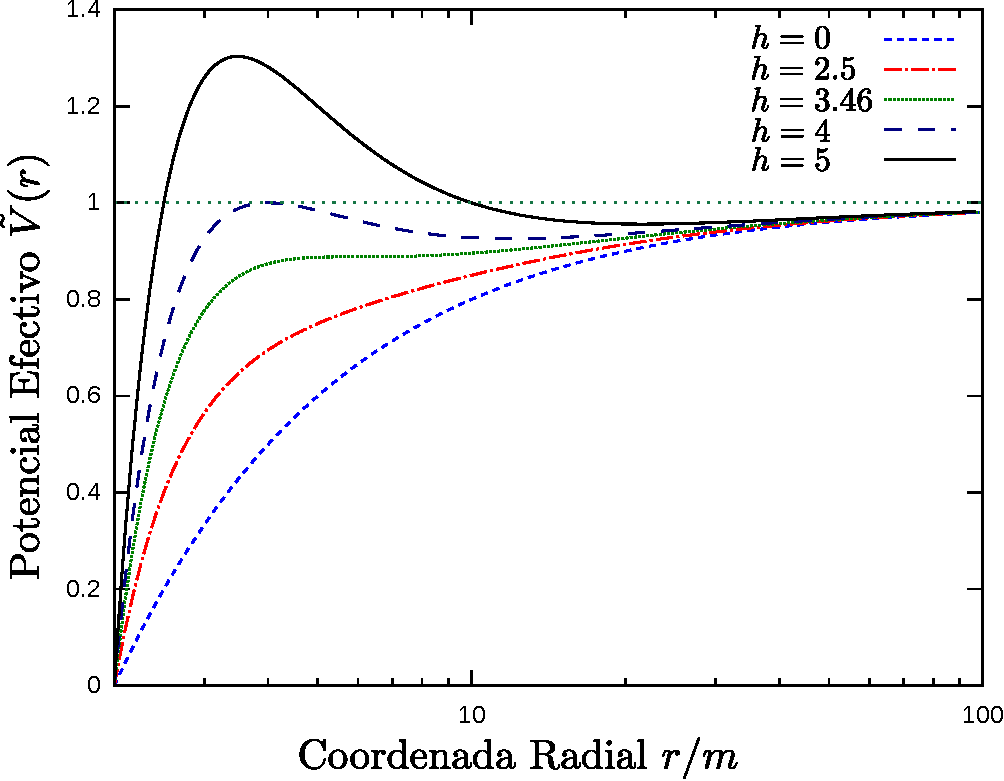
\includegraphics[height=6cm,angle=0]{fig/fig-potencial-efectivo-01.pdf}
\caption{Potencial Efectivo (escala logar'itmica en $r$).} \label{fpe}
\end{center}
\end{figure}

Si $h>2\sqrt{3}$ el potencial tiene entonces un m'aximo en $r=r_A$ y un m'inimo en $r=r_B$. Si $h=2\sqrt{3}$ ambos puntos convergen en un punto de inflexi'on, $r_A=r_B$, y si $h<2\sqrt{3}$ no existen extremos locales.

De acuerdo a lo anterior, existen varios tipos de 'orbitas posibles, dependiendo de los valores de $k$ y $h$:

\begin{itemize}
 \item Si $h<2\sqrt{3}$ y $k<1$ el movimiento radial es acotado, con un m'aximo $r_{\rm max}$ determinado por la igualdad $\tilde{V}(r_{\rm max})=k^2$, pero no existe un m'inimo, de modo que en estos casos la part'icula finalmente cae hacia el cuerpo central.
\item Si $h<2\sqrt{3}$ y $k>1$ la trayectoria no est'a acotada en $r$, correspondiendo a una part'icula que viene desde el infinito y cae hacia el cuerpo central, o que escapa desde 'este hasta el infinito.
\item Si $h>2\sqrt{3}$ y $k^2>\tilde{V}(r_A)$ tenemos una situaci'on similar al caso anterior ($h<2\sqrt{3}$ y $k>1$).
\item Si $h>2\sqrt{3}$ y $k^2=\tilde{V}(r_A)$ existen en principio 'orbitas circulares, con $r=r_{\rm c}=\text{cte.}$, tal que $\tilde{V}(r_{\rm c})=k^2$, pero 'estas son \textit{inestables}. Ver \eqref{ddotr}.
\item Si $h>2\sqrt{3}$, $\tilde{V}(r_B)<k^2<\tilde{V}(r_A)$ y $k>1$ existen 'orbitas no ligadas, donde $r$ puede variar desde un valor m'inimo $r_{\rm min}$ (tal que $\tilde{V}(r_{\rm min})=k^2$, $r_{\rm min}>r_A$) hasta el infinito. Ejemplo de este caso son part'iculas que vienen del infinito, son deflectadas por el cuerpo central y escapan nuevamente al infinito. En este caso son tambi'en posibles 'orbitas que caen inevitablemente al cuerpo central.
\item Si $h>2\sqrt{3}$, $\tilde{V}(r_B)<k^2<\tilde{V}(r_A)$ y $k<1$ existen 'orbitas ligadas, cuyas coordenadas radiales var'ian entre $r_{\rm min}$ y $r_{\rm max}$, con $\tilde{V}(r_{\rm min})=\tilde{V}(r_{\rm max})=k^2$.
\item Si $h>2\sqrt{3}$ y $k^2=\tilde{V}(r_B)$ existen 'orbitas circulares estables, con $r=r_{\rm c}=\text{cte.}$, tal que $\tilde{V}(r_{\rm c})=k^2$.
\item Si $h>2\sqrt{3}$ y $k^2<\tilde{V}(r_B)$ tenemos una situaci'on similar al primer caso aqu'i listado ($h<2\sqrt{3}$ y $k<1$).
\end{itemize}

\subsubsection{'Orbitas circulares}
De acuerdo a la clasificaci'on anterior, estudiamos aqu'i el caso en que $h>2\sqrt{3}$ y $k^2=\tilde{V}(r_B)$. Usando (\ref{rAB}b) encontramos (luego de algo de 'algebra) que las constantes de movimiento apropiadas a un movimiento circular estable deben satisfacer la relaci'on siguiente
% \begin{equation}
%  k^2={\frac {2\left(h^2+h\sqrt{h^2-12}-4\right)^2} {h\left(h+\sqrt{h^2-12}\right)^3}}.
% \end{equation}
\begin{equation}
h_{\rm c}=\frac{r_{\rm c}}{\sqrt{m(r_{\rm c}-3m)}}, \qquad  k_{\rm c}=\frac{\left(1-\frac{2m}{r_{\rm c}}\right)}{\sqrt{1-\frac{3m}{r_{\rm c}}}}.
\end{equation}

Usamos (\ref{kh}a)  para expresar $\dot{t}$ en t'erminos de las constantes de movimiento (recuerde que elegimos $\theta=\pi/2$):
% \begin{equation}
%  \dot{t}_{\rm c}=\frac{k}{1-\frac{2m}{r}}=\sqrt{\frac{2h}{h+\sqrt{h^2-12}}}.
% \end{equation}
\begin{equation}
 \dot{t}_{\rm c}=\frac{1}{\sqrt{1-\frac{3m}{r_{\rm c}}}}.
\end{equation}
Similarmente, a partir de (\ref{kh}b) podemos evaluar $\dot\varphi$ en t'erminos de las constantes de movimiento,
% \begin{equation}
%  \dot\varphi_{\rm c}=\frac{hmc}{r_{\rm c}^2}=\frac{4c}{mh}\frac{1}{\left(h+\sqrt{h^2-12}\right)^2}.
% \end{equation}
\begin{equation}
 \dot\varphi_{\rm c}=\frac{c}{r_{\rm c}}\sqrt{\frac{m}{r_{\rm c}-3m}}.
\end{equation}
Ya que tanto $ \dot{t}_{\rm c}$ como $ \dot\varphi_{\rm c}$ son constantes, podemos integrar las ecuaciones de movimiento directamente, obteniendo
\begin{equation}
 x^\mu(\tau)=( \dot{t}_{\rm c}\tau,r_{\rm c},\frac{\pi}{2}, \dot\varphi_{\rm c}\tau).
\end{equation}
La menor 'orbita circular estable (``innermost stable circular orbit'', ISCO), se obtiene, de acuerdo a (\ref{rAB}b), en el l'imite $h\to 2\sqrt{3}$. En este caso
\begin{equation}
 r_{\rm c}=6\,m,
\end{equation}
y
\begin{equation}
 k_{_{\rm ISCO}}= \frac{2\sqrt{2}}{3}, \qquad \dot{t}_{_{\rm ISCO}}=\sqrt{2}, \qquad \dot\varphi_{_{\rm ISCO}}=\frac{\sqrt{3}}{18}\frac{c}{m}.
\end{equation}
Por lo tanto, a diferencia del caso newtoniano, \textbf{\textit{la teor'ia gravitacional de Einstein predice un l'imite para la existencia de 'orbitas circulares estables}}. En la teor'ia newtoniana, ellas existen para cada valor de $r>0$, en RG s'olo pueden existir para $r_{\rm c}\ge6m$.

\subsubsection{'Orbitas ligadas no-circulares}
Este es el caso en que $h>2\sqrt{3}$, $\tilde{V}(r_B)<k^2<\tilde{V}(r_A)$ y $k<1$. Para analizar la forma de la trayectoria es conveniente considerar c'omo cambia la coordenada radial en t'erminos de la angular, $r=r(\varphi)$. Para esto, realizamos el cambio de variables correspondiente, de modo que
\begin{equation}
r':=\frac{dr}{d\varphi}=\frac{\frac{dr}{d\tau}}{\frac{d\varphi}{d\tau}}=\frac{
\dot{r}}{\dot{\varphi}}.
\end{equation}
Usando ahora (\ref{kh}b) podemos escribir
\begin{equation}
\dot{r} =\frac{hmc}{r^2}r', \qquad \ddot{r}=\frac{h^2m^2c^2}{r^4}\left[-\frac{2}{r}r'^2+r''\right].
\end{equation}
Adicionalmente, la soluci'on de las ecuaciones de movimiento es m'as simple, tal como en el caso newtoniano, definiendo la variable auxiliar
\begin{equation}
 u:=\frac{1}{r},
\end{equation}
de modo que
\begin{equation}
r' =-\frac{1}{u^2} u',  \qquad r''=\frac{2}{u^3}u'^2-\frac{1}{u^2}u''.
\end{equation}
Con estos cambios, la ecuaci'on (\ref{uuc22})  se transforma en
\begin{equation}
h^2m^2u'^2-k^2+(1-2mu)(1+h^2m^2u^2)=0.
\end{equation}
Derivando esta relaci'on y considerando el caso no circular, es decir $u'\neq 0$, obtenemos
\begin{equation}
u''+u=\frac{1}{mh^2}+3m\,u^2 \label{ecuGR}.
\end{equation}
La ecuaci'on newtoniana correspondiente, ver (\ref{EC1}),  es
\begin{equation}
 u''+u=\frac{1}{mh^2},\label{ecrNew}
\end{equation}
con soluci'on
\begin{equation}
 u_0(\varphi)=\frac{1}{mh^2}\left(1+e\cos\varphi\right).
\end{equation}
% Por lo tanto, el valor m'aximo de $u$ es del orden $u_{\rm max}\approx \frac{1}{mh^2}$.
En estas condiciones, el t'ermino ``extra'' en el lado derecho de (\ref{ecuGR}) es mucho m'as peque\~no que el t'ermino ``newtoniano''. En efecto, definiendo la variable adimensional
\begin{equation}
 w:=mh^2\,u.
\end{equation}
Entonces (\ref{ecuGR})  es equivalente a
\begin{equation}
w''+w=1+\epsilon\,w^2 ,\label{ecwGR}
\end{equation}
con
\begin{equation}
 \epsilon:=\frac{3}{h^2}.
\end{equation}
Usando (\ref{kh}b) encontramos que, en el caso de cuerpos orbitando en campos
d'ebiles (como es el caso en nuestro sistema solar),
\begin{equation}
 \epsilon=\frac{3m^2c^2}{r^4\dot\varphi^2}\approx\frac{3m^2c^2}{r^2v_\varphi^2}
 \approx 3\frac{m^2}{r^2}\frac{c^2}{v_\varphi^2}\approx 3\frac{m}{r}\ll 1.
\end{equation}
En particular para Mercurio $\epsilon\approx 10^{-7}$. Por otro lado $w\approx
1$.

Usando el m'etodo perturbativo, postulamos la siguiente expansi'on para la soluci'on de (\ref{ecuGR}):
\begin{equation}
w(\varphi,\epsilon)=w_0(\varphi)+\epsilon\, w_1(\varphi) +\epsilon^2\,w_2(\varphi)+\mathcal{O}(\epsilon^3), \label{expw}
\end{equation}
donde la soluci'on ``no perturbada'' es
\begin{equation}
 w_0(\varphi)=1+e\cos\varphi ,
\end{equation}
y donde $w_1$, $w_2$ se suponen de orden de magnitud 1. Reemplazando la expansi'on (\ref{expw}) en (\ref{ecuGR}) e igualando t'erminos del mismo orden en potencias de $\epsilon$, obtenemos la siguiente ecuaci'on para la primera perturbaci'on:
\begin{eqnarray}
 w_1''+w_1&=&1+2e\cos\varphi+e^2\cos^2\varphi \\
&=& (1+\frac{e^2}{2})+2e\cos\varphi+\frac{e^2}{2}\cos(2\varphi). \label{ecw1}
\end{eqnarray}
Esta es una ecuaci'on tipo oscilador arm'onico forzado, donde el t'ermino forzante es la superposici'on de un t'ermino constante, un \textit{t'ermino resonante}, y un t'ermino peri'odico no resonante. Su soluci'on es del tipo
\begin{equation}
 w_1(\varphi)=A+B\varphi\sen\varphi+C\cos(2\varphi).
\end{equation}
Reemplazando esta soluci'on general en (\ref{ecw1}) podemos determinar las constantes involucradas:
\begin{equation}
 A=1+\frac{e^2}{2}, \qquad B=e, \qquad C=-\frac{e^2}{6}.
\end{equation}
Con esto, la soluci'on de la ecuaci'on (\ref{ecuGR}) a primer orden en $\epsilon$ adopta la forma:
\begin{equation}\label{solucasi}
 u(\varphi)=\frac{1}{mh^2}\left[1+e\cos\varphi+\epsilon\left[\underbrace{
(1+\frac { e^2 } { 2 } )}_\text{pert.
constante}+\underbrace{e\varphi\sen\varphi}_\text{pert. ``secular''}
-\underbrace{\frac{e^2 }{6} \cos(2\varphi)}_\text{pert. peri'odica}\right ]
\right ] +\mathcal{O}(\epsilon^2).
\end{equation}
Usando ahora
\begin{equation}
 \cos(\epsilon\varphi) =1+\mathcal{O}(\epsilon^2), \qquad
\sen(\epsilon\varphi) =\epsilon\varphi+\mathcal{O}(\epsilon^3),
\end{equation}
podemos escribir los t'erminos newtonianos y de perturbaci'on secular como
\begin{equation}
 \cos\varphi+\epsilon\varphi\sen\varphi=\cos\left[(1-\epsilon)\varphi\right]
+\mathcal{O}(\epsilon^2).
\end{equation}
An'alogamente, para la perturbaci'on peri'odica podemos usar
\begin{equation}
 \epsilon\cos(2\varphi)=\epsilon\cos\left[2(1-\epsilon)\varphi\right]+\mathcal{O}(\epsilon^2).
\end{equation}
Con esto podemos expresar nuestra soluci'on como
\begin{equation}\marginnote{Trayectoria perturbada}
 \boxed{u(\varphi)=\frac{1}{mh^2}\left[1+\epsilon(1+\frac { e^2 } { 2 }
)+e\cos\left[(1-\epsilon)\varphi\right] -\frac { e^2
}{6}\epsilon\cos[2(1-\epsilon)\varphi]\right ] +\mathcal{O}(\epsilon^2).} \label{solu1}
\end{equation}
Esta forma de la soluci'on a primer orden tiene la ventaja que revela m'as claramente que la 'orbita (nuevamente, a primer orden en $\epsilon$) \textit{es peri'odica en $\varphi$, pero con un periodo angular distinto de $2\pi$}. Como consecuencia, la 'orbita no se cierra luego de una revoluci'on completa. Este hecho implica en particular un \textit{corrimiento del perihelio de la 'orbita}.

\subsubsection{El Avance del Perihelio de Mercurio}

De (\ref{solu1}) vemos que, a primer orden en $\epsilon$, el periodo angular de la 'orbita no es $2\pi$, sino $2\pi/(1-\epsilon)>2\pi$. Esto significa que la 'orbita retornar'a a una misma distancia dada del centro de fuerzas (por ejemplo, el perihelio) s'olo luego de realizar algo m'as que una rotaci'on completa en torno al centro de fuerzas, en un 'angulo de $2\pi/(1-\epsilon)$. En otras palabras, el \textit{corrimiento angular} de la 'orbita es dado por
\begin{figure}[H]
 \begin{center}
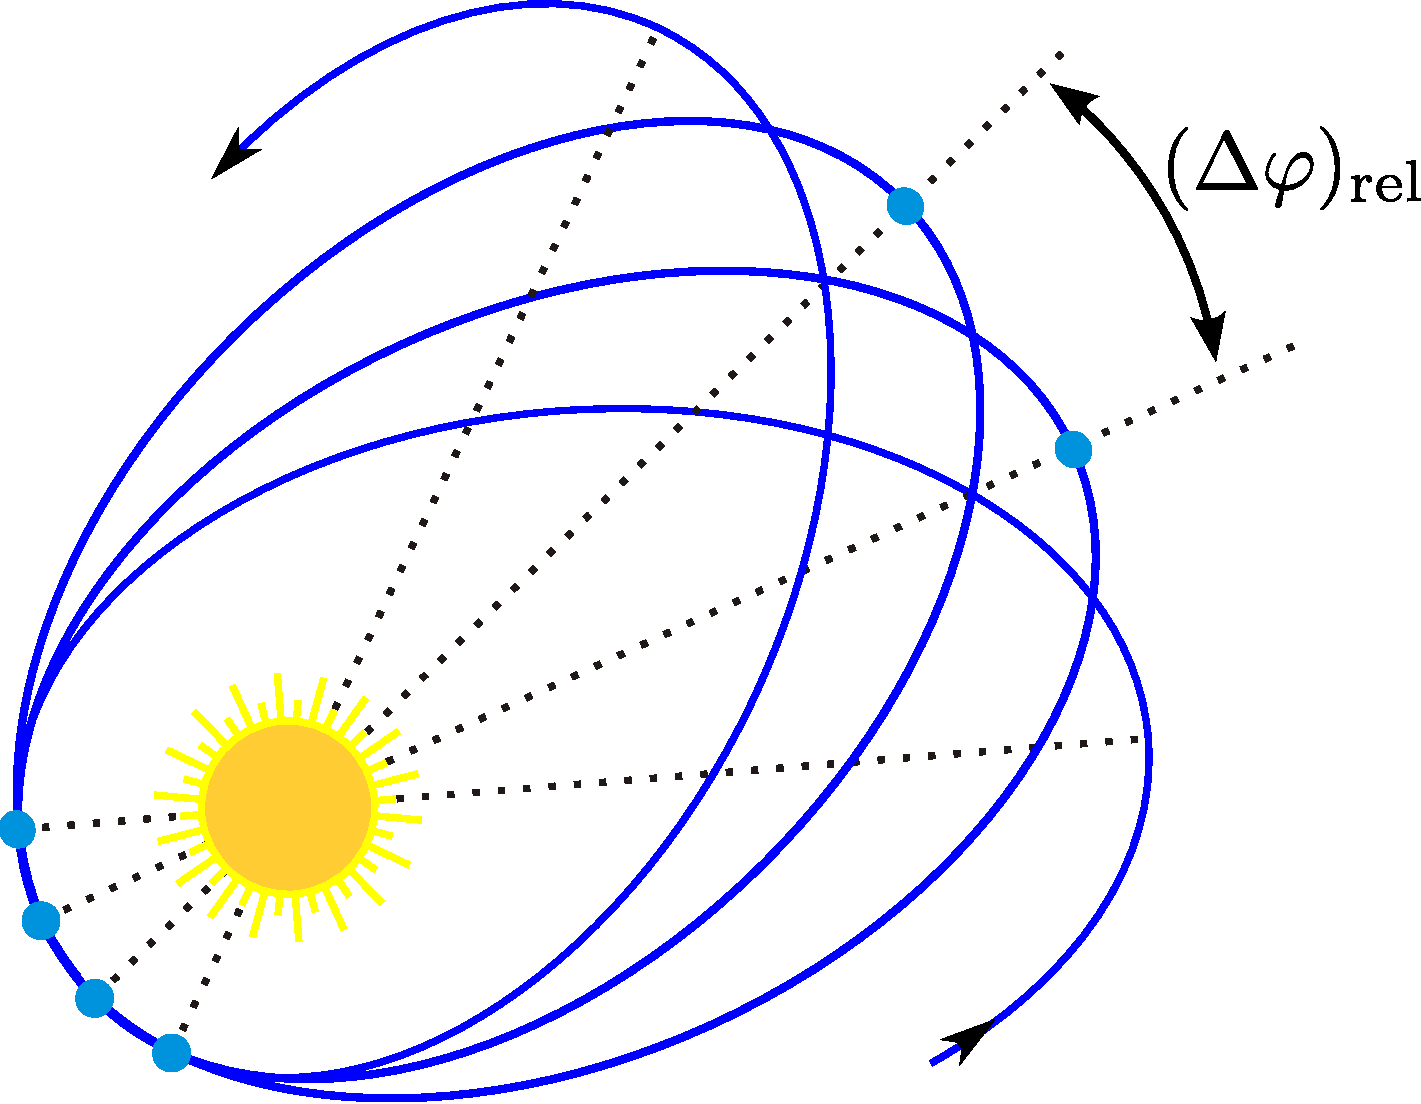
\includegraphics[height=5cm]{fig/fig-precesion-02.pdf}
\caption{Corrimiento del perihelio (adaptada a partir de \href{http://en.wikipedia.org/wiki/File:Perihelion_precession.svg}{esta} figura original).}
\end{center}
\end{figure}
\begin{equation}
\Delta\varphi=\frac{2\pi}{1-\epsilon}-2\pi=2\pi\epsilon+\mathcal{O}(\epsilon^2)=\frac{6\pi}{h^2}+\mathcal{O}(\epsilon^2).
\end{equation}
Podemos expresar $\epsilon$ en t'erminos del semieje mayor y la excentricidad de la 'orbita, ya que
\begin{equation}
a:=\frac{r_{\rm min}+r_{\rm max}}{2}=\frac{mh^2}{1-e^2}+\mathcal{O}(\epsilon).
\end{equation}
As'i obtenemos, a primer orden,
\begin{equation}
 (\Delta\varphi)_{\rm rel}\approx\frac{6\pi m}{a(1-e^2)},
\end{equation}
o, en t'erminos de la masa del cuerpo central:
\begin{equation}\marginnote{Avance periastro}
 \boxed{(\Delta\varphi)_{\rm rel}\approx \frac{6\pi GM}{ac^2(1-e^2)}.}
\end{equation}

Esta expresi'on fue derivada por Einstein en 1915 y aplicada al caso de la 'orbita de Mercurio \cite{Einstein15}. El avance del perihelio de Mercurio era un fen\'omeno conocido antes de la formulaci'on de la teor\'ia de la Relatividad General, ya que Le Verrier \cite{LeVerrier} public'o en 1859 sus observaciones y c'alculos en los que dejaba en evidencia un \textit{avance an'omalo} de $\approx 45\pm 5$''/siglo  (valor citado por Einstein en \cite{Einstein15}). Este valor an'omalo es el resultante de restar el valor esperado de acuerdo a la teor'ia de newton al valor observado\footnote{Luego de tambi'en sustraer el efecto de la \href{http://en.wikipedia.org/wiki/Axial_precession}{precesi\'on general}. Ver referencia \cite{Clemence47} para m'as detalles.} (de la 'epoca) de $\approx 574$''/siglo.  De acuerdo a Clemence (1947) \cite{Clemence47} las mayores contribuciones newtonianas al corrimiento del perihelio de Mercurio son: Venus ($\approx 278$''/siglo), J'upiter ($\approx 153$''/siglo), la Tierra ($\approx 90$''/siglo), Saturno ($\approx 7$''/siglo), Marte ($\approx 2.5$''/siglo), Urano ($\approx 0.14$''/siglo), Neptuno ($\approx 0.042$''/siglo). Con esto, el corrimiento an'omalo asciende a $\approx 43$''/siglo, valor no pod'ia ser calculado usando la teor'ia newtoniana, y que fue entonces explicado por la nueva teor'ia de Einstein.

Para el caso de Mercurio\footnote{Ver, por ejemplo, \url{http://nssdc.gsfc.nasa.gov/planetary/factsheet/mercuryfact.html}.}  $a\approx 57.91\times 10^6\text{\,km}$, $e\approx 0.2056$. Adem'as, $GM_\odot/c^2\approx 1.48\text{\,km}$. Con esto, la predicci'on relativista para el corrimiento del perihelio de Mercurio asciende a $(\Delta\varphi)_{\rm rel}\approx 5.03\times 10^{-7}{\,\rm rad/rev}\approx 0.104$''/rev. Como el periodo orbital de Mercurio es $T\approx 87.97\text{ d'ias}\approx 2,41\times 10^{-3}\text{ siglo}$, entonces  $(\Delta\varphi)_{\rm rel}\approx 43$''/siglo. El valor aceptado actualmente para la predicci'on relativista es de $(\Delta\varphi)_{\rm rel}\approx 42.98$''/siglo, ver \cite{NW86}. Este resultado est'a en completo acuerdo con el resultado observacional aceptado actualmente, de $42.98(1.000\pm 0.001)$''/siglo. Ver \cite{Will06}, secci'on 3.5, para detalles adicionales.

La predicci'on de RG para el corrimiento del perihelio ha sido adem'as verificada en nuestro sistema solar para las 'orbitas de Venus, la Tierra y Marte. En esos casos el corrimiento relativista asciende a aproximadamente $8.65$''/siglo, $3.85$''/siglo y $1.36$''/siglo, respectivamente \cite{OR94}. Una de las mejores verificaciones actualmente disponible es la correspondiente al corrimiento del perihelio de la 'orbita del pulsar binario de Hulse \& Taylor PRS 1913+16, para el cual el corrimiento es de aproximadamente 13''/rev (y el periodo de rotaci'on es algo menor que 8 horas!) \cite{Taylor93}.

\subsection{Desv'io de la luz}

En este caso, realizaremos un c'alculo similar al correspondiente a trayectorias tipo tiempo, con la diferencia que la ecuaci'on de la geod'esica, usando un par'ametro arbitrario $\lambda$, adopta la forma
\begin{equation}
\frac{d^2x^\mu}{d\lambda^2}+\Gamma^\mu_{\nu\rho}\frac{dx^\nu}{d\lambda}\frac{dx^\rho}{d\lambda}=f(\lambda)\frac{dx^\mu}{d\lambda},
\end{equation}
De este modo las ecuaciones de movimiento toman la forma (aqu'i denotamos $\dot{(\ \,)}:={d(\ \,)}/{d\lambda}$):
\begin{eqnarray}
\frac{1}{\left(1-\frac{2m}{r}\right)}\frac{d\ }{d\lambda}\left[\left(1-\frac{2m}{r}\right)\dot{t}\right]&=&f\,\dot{t}, \label{egSl0}\\
\ddot{r}+\frac{mc^2(r-2m)}{r^3}\,\dot{t}^2-\frac{m}{r\left(
r-2m\right) }\,\dot{r}^2-(r-2m) \left[ \dot{\theta}^2+\sen
^2\theta \dot{\varphi}^2\right] &=&f\,\dot{r}, \label{egSl1}\\
\ddot{\theta}+\frac{2}{r}\dot{r}\dot{\theta}-\sen \theta \cos \theta
\dot{\varphi}^2 &=&f\,\dot{\theta}, \label{egSl2}\\
\frac{1}{r^2\sen^2\theta}\frac{d\ }{d\lambda}\left[r^2\sen^2\theta\dot{\varphi}\right] &=&f\,\dot{\varphi}.\label{egSl3}
\end{eqnarray}%
Note que hemos factorizado los t'erminos al lado izquierdo de (\ref{egSl0}) y (\ref{egSl3}). Nuevamente, el movimiento est'a confinado a un plano, que podemos elegir como el plano ecuatorial, es decir, con $\theta(\lambda)=\pi/2$. Verificamos que esta soluci'on para $\theta$ satisface (\ref{egSl2}). Tal como en el caso tipo tiempo, finalmente nos concentraremos en la forma de la trayectoria. Por esto, elegiremos como par'ametro al 'angulo $\varphi$, es decir, $\lambda:=\varphi$. Con esto, $\dot{\varphi}=1$ y podemos determinar la funci'on $f$ correspondiente a partir de (\ref{egSl3}):
\begin{equation}
f=\frac{d\ }{d\varphi}\ln\left[r^2\right]=\frac{2}{r}r'.
\end{equation}
Introduciendo esta funci'on en (\ref{egSl0}) obtenemos, luego de una simple 'algebra,
\begin{equation}
\frac{d\ }{d\varphi}\ln\left[\frac{r^2}{\left(1-\frac{2m}{r}\right)t'}\right]=0,
\end{equation}
que expresa el hecho que existe una cantidad conservada en el movimiento:
\begin{equation}\label{ccl}
 \frac{r^2}{\left(1-\frac{2m}{r}\right)}\frac{d\varphi}{dt}=:\frac{c}{\alpha}.
\end{equation}
Aqu'i, para conveniencia posterior, hemos introducido $\alpha$ como constante, con dimensiones $[\alpha]=L^{-1}$, determinada por las condiciones iniciales del movimiento.

Por otro lado, la ecuaci'on radial (\ref{egSl1}) se reduce a
\begin{equation}
 r''+\frac{mc^2(r-2m)}{r^3}\,t'^2-\frac{m}{r\left(r-2m\right) }\,r'^2-(r-2m) =\frac{2}{r}r'^2. \label{ecr2l}
\end{equation}

Tal como en el caso tipo tiempo, esta ecuaci'on puede derivarse de la ecuaci'on de primer orden, en este caso, de la condici'on $g_{\mu\nu}\dot{x}^\mu\dot{x}^\nu=0$. Esta condici'on implica que
\begin{equation}
\left(1-\frac{2m}{r}\right)c^2\left(\frac{dt}{d\varphi}\right)^2-\frac{1}{\left(1-\frac{2m}{r}\right)}\left(\frac{dr}{d\varphi}\right)^2-r^2=0. \label{e2orl}
\end{equation}
Usando (\ref{ccl}) para expresar $dr/d\varphi$ en t'erminos de $r$ y la constante de moviento $\alpha$, la condici'on (\ref{e2orl}) se reduce a
\begin{equation}\label{ecrpf}
 r'^2+r^2-2mr-\alpha^2r^4=0,
\end{equation}
donde $'$ denota la derivada con respecto a $\varphi$.

Introduciendo ahora $u:=1/r$ transformamos esta ecuaci'on en
\begin{equation}
 u'^2+u^2=\alpha^2+2mu^3. \label{ecul0}
\end{equation}
Derivando esta ecuaci'on llegamos a una ecuaci'on de segundo orden en las derivadas de $u$ que, tal como en el caso tipo tiempo, es equivalente a la ecuaci'on (\ref{ecr2l}):
\begin{equation}
 u''+u=3mu^2. \label{ecglrg}
\end{equation}
Esta ecuaci'on es la an'aloga a (\ref{ecuGR}). Tal como en el caso anterior, el t'ermino introducido por la teor'ia de RG es $3mu^2$. Puede comprobarse que la ecuaci'on newtoniana, que corresponde al l'imite $m\to 0$, es
\begin{equation}
 u''+u=0, \label{ecglnew}
\end{equation}
y que \textit{sus soluciones son l'ineas rectas}. En efecto, una soluci'on general de (\ref{ecuGR}) puede expresarse en la forma siguiente:
\begin{equation}
 u_0(\varphi)=\frac{1}{D}\sen(\varphi-\varphi_0),
\end{equation}
donde $D$ es una constante con dimensiones de longitud y $\varphi_0$ una constante angular. Entonces tendremos que
\begin{equation}
x=r\cos\varphi=D\frac{\cos\varphi}{\sen(\varphi-\varphi_0)}, \qquad
y=r\sen\varphi=D\frac{\sen\varphi}{\sen(\varphi-\varphi_0)}.
\end{equation}
Una simple 'algebra permite entonces relacionar $x$ con $y$, obteniendo
\begin{equation}
 y=\frac{D}{\cos\varphi_0}+\left(\tan\varphi_0\right)x. \label{recta}
\end{equation}
La expresi'on (\ref{recta}) describe una recta en el plano $x-y$, siendo $D$ la \textit{distancia m'inima de la recta al origen} y $\varphi_0$ el 'angulo que forma la recta con el eje $x$. Ver figura \ref{fig:recta}.
\begin{figure}[H]
 \begin{center}
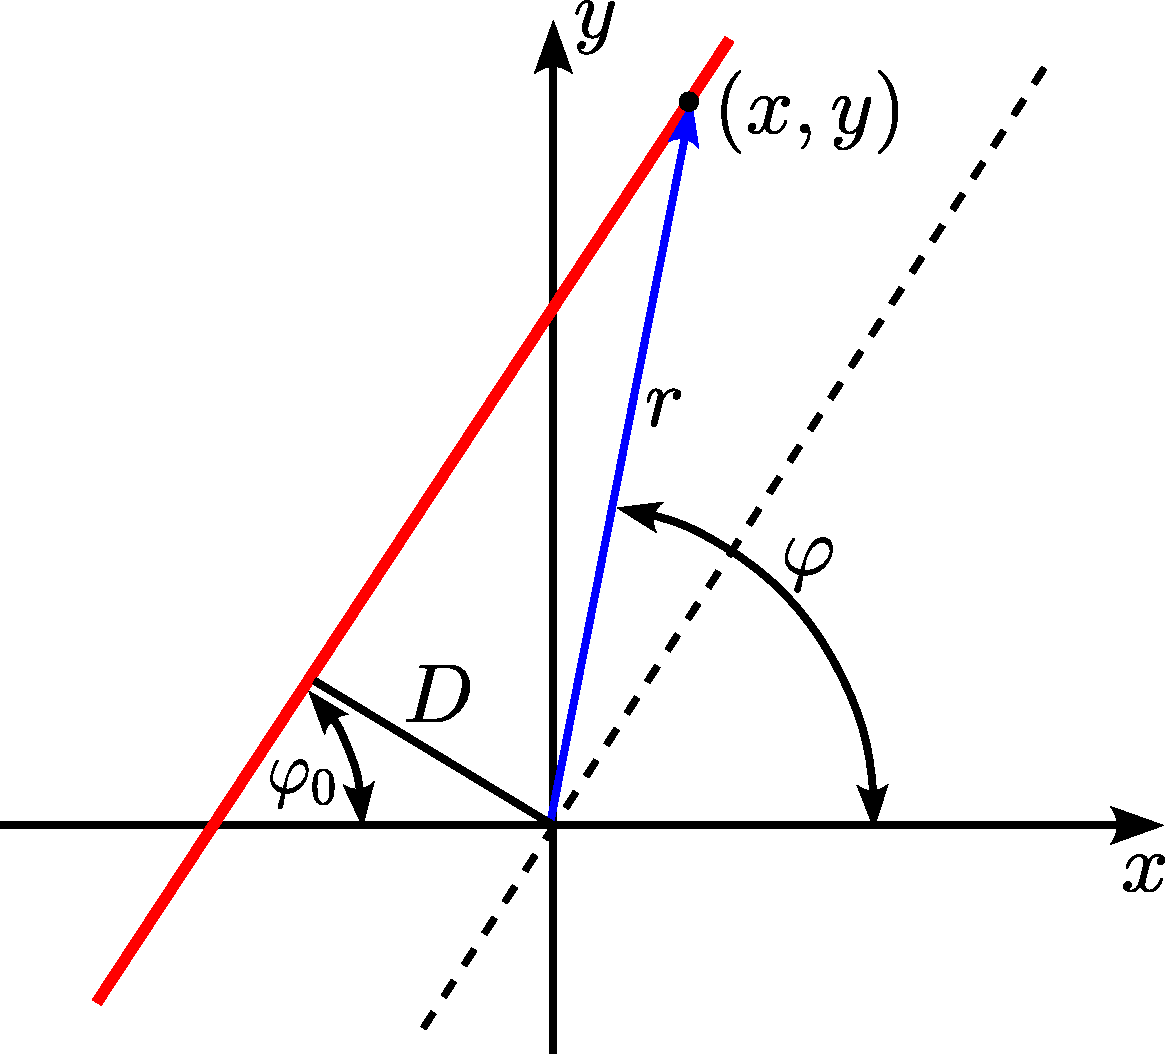
\includegraphics[height=6cm]{fig/fig-recta.pdf}
\caption{Soluci'on newtoniana para el movimiento del rayo de luz.}
\label{fig:recta}
\end{center}
\end{figure}

Determinaremos nuevamente una soluci'on aproximada de (\ref{ecglrg}). Primero definimos la variable adimensional $w(\varphi):=Du(\varphi)$. Con esto (\ref{ecglrg}) se transforma en
\begin{equation}
 w''+w=\epsilon\, w^2, \label{ecglrgw}
\end{equation}
que tiene como soluci'on ``sin perturbar'' a
\begin{equation}
 w_0(\varphi)=\sen(\varphi-\varphi_0). \label{w0l}
\end{equation}
La constante $\epsilon$ tiene el valor
\begin{equation}
 \epsilon:=\frac{3m}{D},
\end{equation}
que es mucho menor que 1, ya que suponemos que el rayo de luz pasa suficientemente lejos del centro de fuerzas de modo que $D\gg m$. Suponemos adem'as que $w\approx 1$. Con estos ingredientes determinaremos una soluci'on perturbativa de la forma (\ref{expw}), con $w_0$ dado por (\ref{w0l}). Introduciendo la expansi'on (\ref{expw}) y usando (\ref{w0l}) encontramos la ecuaci'on para la primera perturbaci'on $w_1$:
\begin{equation}
 w_1''+w_1=\sen^2(\varphi-\varphi_0). \label{ecw1l}
\end{equation}
La soluci'on general de esta ecuaci'on es de la forma
\begin{equation}
 w_1(\varphi)=A+B\cos(\varphi-\varphi_0+\beta)+C\cos^2(\varphi-\varphi_0).
\end{equation}
Substituyendo esta expresi'on en (\ref{ecw1l}) encontramos que $A=C=1/3$, mientras que las constantes $B$ y $\beta$ pueden adoptar valores arbitrarios. Sin embargo, sin p'erdida de generalidad es posible elegir\footnote{En efecto, si $B\neq 0$ y $\beta\neq 0$, la soluci'on puede reescribirse, \textit{a primer orden en} $\epsilon$ como
\begin{equation*}
u(\varphi)=\frac{1}{\tilde{D}}\left[\sen(\varphi-\tilde{\varphi}_0)+\frac{m}{\tilde{D}}\left(1+\cos^2(\varphi-\tilde{\varphi_0})\right)\right]+\mathcal{O}(\epsilon^2),
\end{equation*}
con $\tilde{D}:=D/(1-\epsilon B\sen\beta)$ y $\tilde{\varphi}_0:=\varphi_0-\epsilon B\cos\beta$. Esta expresi'on es equivalente a (\ref{solw1l}).} $B=\beta=0$. As'i, nuestra soluci'on a primer orden adopta la forma siguiente:
\begin{equation}\marginnote{Soluci'on pertubada rayo de luz}
 \boxed{u(\varphi)=\frac{1}{D}\left[\sen(\varphi-\varphi_0)+\frac{m}{D}\left[1+\cos^2(\varphi-\varphi_0)\right]\right]+\mathcal{O}(\epsilon^2).} \label{solw1l}
\end{equation}
Para calcular el \textit{'angulo de desv'io} de la luz, $\delta$, necesitamos los 'angulos $\delta_1$ y $\delta_2$ en que la trayectoria se desv'ia de la recta no perturbada, para $t\to -\infty$ y $t\to +\infty$, respectivamene. Estos 'angulos corresponden a un 'angulo inicial $\varphi_{\rm i}=\varphi_0+\pi+\delta_1$ y final $\varphi_{\rm f}=\varphi_0-\delta_2$, y pueden ser determinados por la condici'on que en cada caso $r\to\infty$ o, equivalentemente $u=0$. El 'angulo total de desv'io es entonces $\delta=\delta_1+\delta_2$. Reemplazamos por tanto $\varphi=\varphi_{\rm i}=\varphi_0+\pi+\delta_1$ en la condici'on $u(\varphi_{\rm i})$ obtenemos, a primer orden en $\delta_1$:
\begin{eqnarray}
 0&=&u(\varphi_{\rm i})\\
&=&\frac{1}{D}\left[\sen(\pi+\delta_1)+\frac{m}{D}\left(1+\cos^2(\pi+\delta_1)\right)\right] \\
&=&\frac{1}{D}\left[-\sen\delta_1+\frac{m}{D}\left(1+\cos^2\delta_1)\right)\right] \\
&=&\frac{1}{D}\left[-\delta_1+\frac{m}{D}\left(1+1\right)\right]+\mathcal{O}(\delta_1^2).
\end{eqnarray}
Por lo tanto, obtenemos,
\begin{equation}
 \delta_1=\frac{2m}{D}.
\end{equation}
Similarmente, para $\varphi_{\rm f}=\varphi_0-\delta_2$ encontramos:
\begin{eqnarray}
 0&=&u(\varphi_{\rm f})\\
&=&\frac{1}{D}\left[-\sen\delta_2+\frac{m}{D}\left(1+\cos^2\delta_2\right)\right] \\
&=&\frac{1}{D}\left[-\delta_2+\frac{m}{D}\left(1+1\right)\right]+\mathcal{O}(\delta_2^2),
\end{eqnarray}
de modo que
\begin{equation}
 \delta_2=\frac{2m}{D}.
\end{equation}
As'i obtenemos que el 'angulo total de desv'io es
\begin{equation}
 \delta\approx\frac{4m}{D},
\end{equation}
o, en t'erminos de la masa del cuerpo central\footnote{Note que, en estricto rigor, la constante $D$ no es exactamente el valor m'inimo de la coordenada radial en la trayectoria del fot'on. La soluci'on (\ref{solw1l}) implica que el m'inimo de $r$ (m'aximo de $u$) se obtiene para $\varphi=\varphi_0+\pi/2$, y que a primer orden $r_{\rm min}=D/(1+m/D)\approx D-m$. La diferencia entre $D$ y $r_{\rm min}$ es por esto muy peque\~na y despreciable en el contexto de de la aproximaci'on usada.\label{fn8}},
\begin{equation}\marginnote{'Angulo de desv'io} \label{dlRG}
 \boxed{\delta\approx\frac{4GM}{c^2D}.}
\end{equation}

En 1911 Einstein presenta un primer c'alculo para el 'angulo de desv'io de la luz en un campo gravitacional, basado en el principio de equivalencia, pero a'un en el contexto de la teor'ia newtoniana. El valor calculado de esta forma resulta ser \textit{la mitad} del 'angulo \eqref{dlRG} que predice teor'ia de Relatividad General completa. Ver \cite{Einstein11}, p'agina 908. Es interesante notar adem'as que si se considera la teor'ia newtoniana de la gravitaci'on y a los fotones como part'iculas (masivas) que son atraidas por el Sol y que se mueven con rapidez $c$, tambi'en se obtiene el resultado correspondiente a la mitad de \eqref{dlRG}. Ver \cite{Will88} para mayores detalles.  Por otro lado, el resultado \eqref{dlRG} fue presentado por Einstein por primera vez en su paper de 1916 \cite{Einstein16} (ecuaci'on 74, p'agina 822).

Note tambi'en que, de acuerdo a \eqref{dlRG}, la teor'ia de RG predice un 'angulo de desv'io \textit{independiente de la frecuencia de la radiaci'on}.

En el caso de rayos de luz pasando muy cerca de la superficie del Sol\footnote{Ver, por ejemplo, \url{http://nssdc.gsfc.nasa.gov/planetary/factsheet/sunfact.html}.}, $D\approx R_\odot\approx 6.96\times 10^5\text{\,km}$, y entonces
\begin{equation}
\delta_\odot\approx\frac{4GM}{c^2R_\odot}\approx 4\left(\frac{1.48\text{\,km}}{6.96\times 10^5\text{\,km}}\right)\approx 4\times 2.13\times 10^{-6}{\rm\, rad}\approx 8.52\times 10^{-6}{\rm\, rad}\approx 1.75\text{''}.
\end{equation}

La observaci'on de este efecto constituy'o la \textit{primera verificaci'on experimental de una predicci'on} de la teor'ia de gravitaci'on de Einstein. El desv'io de la luz fue medido en Mayo de 1919 por Eddington\footnote{Sir Arthur Eddington (1882-1944) astrof'isico brit'anico. Ver, por ejemplo, \url{http://es.wikipedia.org/wiki/Arthur_Stanley_Eddington}.} y colaboradores, a partir de mediciones 'opticas de las posiciones de estrellas cercanas al Sol, medidas durante un eclipse total de Sol, observado desde las islas atl'anticas de Sobral y Principe \cite{DED19}. Estos experimentos obtuvieron un resultado consistente con la predicci'on relativista, pero s'olo con un 30\% de precisi'on. Sin embargo, los resultados s'i permit'ian excluir un resultado nulo o la predicci'on ``cuasi-newtoniana'' (la mitad del valor de RG, es decir, $\approx 0.87$''). Se efectuaron nuevas medidas durante eclipses posteriores. En el del 30 de Junio de 1973 los resultados concordaban con la predicci'on de RG con un error del 10\%. Uno de las mayores fuentes de error en este tipo de observaci'on es causada por la corona solar, que tambi'en curva los rayos que pasan por ella. Actualmente, la precisi'on alcanzada por los sistemas VLBI (Very Large Baseline Interferometry) han permitido mejorar sustancialmente la confirmaci'on observacional de la predicci'on de RG para el desv'io de la luz, con una desviaci'on de 0.1\% \cite{SDLG04,Will06}.

\subsection{Redshift Gravitacional}\label{sec:redshift}
Revisaremos aqu'i la predicci'on para el redshift gravitacional (dilataci'on temporal gravitacional). En particular, derivaremos la expresi'on exacta para el redshift medido por dos observadores ``en reposo'' en el espaciotiempo de Schwarzschild. En particular consideraremos fotones que ``escapan'' del centro de fuerzas de manera radial. En este caso, debido a la simetr'ia esf'erica podemos considerar que los fotones se mueven en trayectorias con $\theta=\pi/2$ y $\varphi=0$.

De la condici'on de curva nula para el fot'on $g_{\mu\nu}dx^\mu dx^\nu=0$ obtenemos
\begin{equation}
 \left(1-\frac{2m}{r}\right)c^2dt^2-\frac{dr^2}{ \left(1-\frac{2m}{r}\right)}=0.
\end{equation}
Por lo tanto,
\begin{equation}
 c\,dt=\pm\frac{dr}{ \left(1-\frac{2m}{r}\right)}.
\end{equation}
Los signos positivo y negativo corresponden a fotones ``escapando desde'' y ``cayendo hacia'' el centro de fuerzas, respectivamente. Para el primer caso, tenemos entonces que
\begin{eqnarray}
 c(t-t_0)&=&\int^r_{r_0}\frac{dr}{\left(1-\frac{2m}{r}\right)} \\
&=&\left.\left(r+2m\ln|r-2m|\right)\right|^r_{r_0} \\
&=&r-r_0+2m\ln\left(\frac{r-2m}{r_0-2m}\right).
\end{eqnarray}
En otras palabras,
\begin{equation} \label{tferf}
 t=t_0+\frac{1}{c}\left[r-r_0+2m\ln\left(\frac{r-2m}{r_0-2m}\right)\right].
\end{equation}
Esta relaci'on define en forma impl'icita la ecuaci'on de la trayectoria, exacta en el espaciotiempo de Schwarzschild, $r(t)$, del fot'on escapando radialmente. Podemos verificar  aqu'i lo usado en la discusi'on del redshift gravitacional en la secci'on (\ref{zg1}): que $(\Delta t)_{\rm e}=(\Delta t)_{\rm r}$. En efecto, si un fot'on es emitido en el evento con coordenadas $x^\mu_{{\rm e},1}=(t_0,r_0,\pi/2,0)$ entonces 'este llega a un punto con coordenada radial $r$ en el evento $x^\mu_{{\rm r},1}=(t,r,\pi/2,0)$, donde $t$ es dado por (\ref{tferf}). Como (\ref{tferf}) es lineal en $t_0$ tendremos que si otro fot'on es enviado desde $r_0$ en el evento $x^\mu_{{\rm e},2}=(t_0+(\Delta t)_{\rm e},r_0,\pi/2,0)$, entonces llegar'a a $r$ en el evento $x^\mu_{{\rm e},2}=(t+(\Delta t)_{\rm e},r,\pi/2,0)$. En otras palabras, $(\Delta t)_{\rm e}=(\Delta t)_{\rm r}$. Este es un resultado general, v'alido para todo espaciotiempo estacionario (es decir, en que la m'etrica es independiente de la coordenada temporal).

Por otro lado, los tiempos propios asociados a observadores ``en reposo'' en el punto de emisi'on y recepci'on, es decir, cuyas l'ineas de mundo tienen coordenada radial constate $r_{\rm e}$ y $r_{\rm r}$ respectivamente, quedan determinados por
\begin{equation}
 ds^2=c^2d\tau^2=\left(1-\frac{2m}{r}\right)c^2dt^2,
\end{equation}
de modo que
\begin{equation}
\Delta\tau_{\rm e}=\sqrt{1-\frac{2m}{r_{\rm e}}}\, (\Delta t)_{\rm e}, \qquad
\Delta\tau_{\rm r}=\sqrt{1-\frac{2m}{r_{\rm r}}}\, (\Delta t)_{\rm r}.
\end{equation}
Con estos ingredientes, obtenemos
\begin{equation}\marginnote{Dilataci'on temporal gravitacional}\label{rgsch}
\boxed{\frac{\Delta\tau_{\rm r}}{\Delta\tau_{\rm e}}=\sqrt{\frac{1-\frac{2m}{r_{\rm r}}}{1-\frac{2m}{r_{\rm e}}}}}.
\end{equation}
Compare esta expresi'on con aquella encontrada en el l'imite de campo d'ebil, expresiones  (\ref{zapp1}) y (\ref{zapp2}).

\subsection{Tiempo de Vuelo (Efecto Shapiro)*}
Aqu'i estudiaremos la predicci'on de la teor'ia de Einstein de la gravitaci'on en lo que respecta al \textit{tiempo de vuelo} de se\~nales luminosas en la m'etrica de Schwarzschild.

Para obtener informaci'on del tiempo de vuelo de una se\~nal luminosa debemos analizar c'omo cambia la coordenada temporal $t$ a lo largo de la l'inea de mundo del rayo de luz.
Usando (\ref{ccl}) podemos escribir
\begin{equation}
\frac{dr}{dt}=\frac{dr}{d\varphi}\frac{d\varphi}{dt}=r'\frac{mc}{\alpha}\left(1-\frac{2m}{r}\right)\frac{1}{r^2}.
\end{equation}
Reemplazando ahora la expresi'on para $r'$ determinada por la relaci'on (\ref{ecrpf}) encontramos que
\begin{equation}
\frac{1}{c}\frac{dr}{dt}=\pm\, I(r),
\end{equation}
donde hemos definido
\begin{equation}
I(r):=\frac{1}{\alpha}\left(1-\frac{2m}{r}\right)\sqrt{\alpha^2+\frac{2m}{r^3}-\frac{1}{r^2}}.
\end{equation}
Ahora aplicamos esta expresi'on al caso en que el fot'on se mueve desde un punto con coordenadas $(ct_T,r_T,\pi/2,\varphi_T)$ hacia el centro de fuerzas, hasta el punto $(ct_0,r_0,\pi/2,\varphi_0)$ de m'aximo acercamiento. En este primer tramo $dr/dt<0$ y entonces
\begin{equation}\label{Dti1}
c\,(t_0-t_T)=-\int^{r_0}_{r_T}\frac{dr}{I(r)}.
\end{equation}
En el segundo tramo, desde $(ct_0,r_0,\pi/2,\varphi_0)$ hasta $(ct_V,r_V,\pi/2,\varphi_V)$, tenemos que $dr/dt>0$ y entonces
\begin{equation}\label{Dti2}
c\,(t_V-t_0)=\int_{r_0}^{r_V}\frac{dr}{I(r)}.
\end{equation}
El intervalo total de coordenada temporal en el proceso de vuelo (``de ida'') es entonces dado por $t_V-t_T$. Usando (\ref{Dti1}) y (\ref{Dti2}) obtenemos
\begin{eqnarray}
c\,(t_V-t_T)&=&\int_{r_0}^{r_V}\frac{dr}{I(r)}-\int^{r_0}_{r_T}\frac{dr}{I(r)} \\
&=&\int_{r_0}^{r_V}\frac{dr}{I(r)}+\int_{r_0}^{r_T}\frac{dr}{I(r)}. \label{cDtI}
\end{eqnarray}
Para evaluar esta expresi'on es necesario escribir $\alpha$ en t'erminos de $r_0=r_{\rm min}$, la coordenada radial m'inima al centro de fuerzas sobre la trayectoria del fot'on. Esta coordenada m'inima se encuentra, ver nota al pie \ref{fn8}, para el 'angulo $\varphi_{\rm min}=\varphi_0+\pi/2$ y satisface $u(\varphi_{\rm min})=1/r_{\rm min}$, $u'(\varphi_{\rm min})=0$, con
\begin{equation}
 r_0=D\left(1-\frac{m}{D}\right)+\mathcal{O}(\epsilon^2).
\end{equation}
Usando estas condiciones, la relaci'on (\ref{ecul0}) implica que
\begin{equation}
 \alpha^2=\frac{1}{r^2_0}\left(1-\frac{2m}{r_0}\right),
\end{equation}
y entonces
\begin{equation}
\alpha=\frac{1}{r_0}\left(1-\frac{m}{r_0}\right)+\mathcal{O}(\epsilon^2).
\end{equation}
Con esto, podemos expresar la funci'on $I(r)$ como
\begin{eqnarray}
 I(r)&=&\frac{1}{\alpha}\left(1-\frac{2m}{r}\right)\sqrt{\alpha^2+\frac{2m}{r^3}-\frac{1}{r^2}} \\
&=&\left(1-\frac{2m}{r}\right)\left(1+\frac{m}{r_0}\right)\sqrt{1-\frac{2m}{r_0}-\frac{2mr_0^2}{r^3}-\frac{r_0^2}{r^2}} +\mathcal{O}(\epsilon^2)\\
&=&\left(1-\frac{2m}{r}+\frac{m}{r_0}\right)\sqrt{1-\frac{r_0^2}{r^2}-\frac{2m}{r_0}\left(1-\frac{r_0^3}{r^3}\right)}+\mathcal{O}(\epsilon^2) \\
&=&\left(1-\frac{2m}{r}+\frac{m}{r_0}\right)\left[\sqrt{1-\frac{r_0^2}{r^2}}+\frac{1}{2\sqrt{1-\frac{r_0^2}{r^2}}}\left(-\frac{2m}{r_0}\right)\left(1-\frac{r_0^3}{r^3}\right)\right] +\mathcal{O}(\epsilon^2)\\
&=&\left(1-\frac{2m}{r}+\frac{m}{r_0}\right)\sqrt{1-\frac{r_0^2}{r^2}}\left[1-\frac{m}{r_0}\frac{\left(1-\frac{r_0^3}{r^3}\right)}{1-\frac{r_0^2}{r^2}}\right] +\mathcal{O}(\epsilon^2)\\
&=&\left(1-\frac{2m}{r}+\frac{m}{r_0}\right)\sqrt{1-\frac{r_0^2}{r^2}}\left[1-\frac{m}{r_0}\frac{\left(1+\frac{r_0}{r}+\frac{r_0^2}{r^2}\right)}{1+\frac{r_0}{r}}\right]+\mathcal{O}(\epsilon^2) \\
&=&\sqrt{1-\frac{r_0^2}{r^2}}\left[1-\frac{mr_0}{r(r+r_0)}-\frac{r_0}{r}\right]+\mathcal{O}(\epsilon^2).
\end{eqnarray}
De esta forma, obtenemos
\begin{equation}
 \frac{1}{I(r)}=\frac{1}{\sqrt{1-\frac{r_0^2}{r^2}}}\left[1+\frac{mr_0}{r(r+r_0)}+\frac{r_0}{r}\right]+\mathcal{O}(\epsilon^2),
\end{equation}
y entonces
\begin{equation}
 \int\frac{dr}{I(r)}=\sqrt{r^2-r_0^2}+2m\ln\left(r+\sqrt{r^2-r_0^2}\right)+m\sqrt{\frac{r-r_0}{r+r_0}}+\mathcal{O}(\epsilon^2).
\end{equation}
Con este resultado podemos evaluar el intervalor $(\Delta t)_{\rm ir}$ de ``ida y regreso''\footnote{Note que este intervalo es en rigor el intervalo de coordenada temporal. El tiempo propio que un observador en $r_T$ registra en el viaje de ida y regreso del fot'on es dado, a primer orden, por $(\Delta\tau)_{\rm ir}=(1-m/r_T)(\Delta t)_{\rm ir}$.} que, de acuerdo a (\ref{cDtI}), es entonces dado por
\begin{eqnarray}
\frac{c}{2}\,(\Delta t)_{\rm ir}&=&\sqrt{r_V^2-r_0^2}+\sqrt{r_T^2-r_0^2}+2m\ln\left[\frac{\left(r_V+\sqrt{r_V^2-r_0^2}\right)\left(r_T+\sqrt{r_T^2-r_0^2}\right)}{r_0^2}\right] \nonumber\\
&&+m\left(\sqrt{\frac{r_V-r_0}{r_V+r_0}}+\sqrt{\frac{r_T-r_0}{r_T+r_0}}\right)+\mathcal{O}(\epsilon^2).
\end{eqnarray}
En el caso que $r_0=R_\odot\ll r_V, r_T$ (``conjunci'on superior'') el efecto es m'aximo:
\begin{eqnarray}
c\,(\Delta t)_{\rm ir}&\approx& 2\left[r_V+r_T+2m\ln\left[\frac{\left(2r_V\right)\left(2r_T\right)}{R_\odot^2}\right]+m\left(1+1\right) \right]\\
&\approx&2\left[(r_V+r_T)+2m\left(1+\ln\left[\frac{4r_Vr_T}{R_\odot^2}\right]\right)\right].
\end{eqnarray}
Para el Sol, Venus y la Tierra $r_V\approx r_T\approx 10^8\text{\,km}$, el segundo t'ermino es $\approx 2\times 10^{-4}\text{\, s}$. Note que hemos despreciado el movimiento de Venus y la Tierra en el periodo en que el rayo de luz realiza su viaje de ida y regreso ($\sim 20\text{ min}$). El uso de este efecto para testear la teor'ia de RG fue propuesto por I. Shapiro en 1964 \cite{Shapiro64} y verificado la predicci'on con precisi'on cada vez mayor en los casos en que la se\~nal enviada ``rebota'' en Mercurio, Venus \cite{Shapiro71}. Este valor ha sido confirmado con una desviaci'on del 5\%. Ver \cite{Wei72} para mayores detalles.
\begin{figure}[H]
\begin{center}
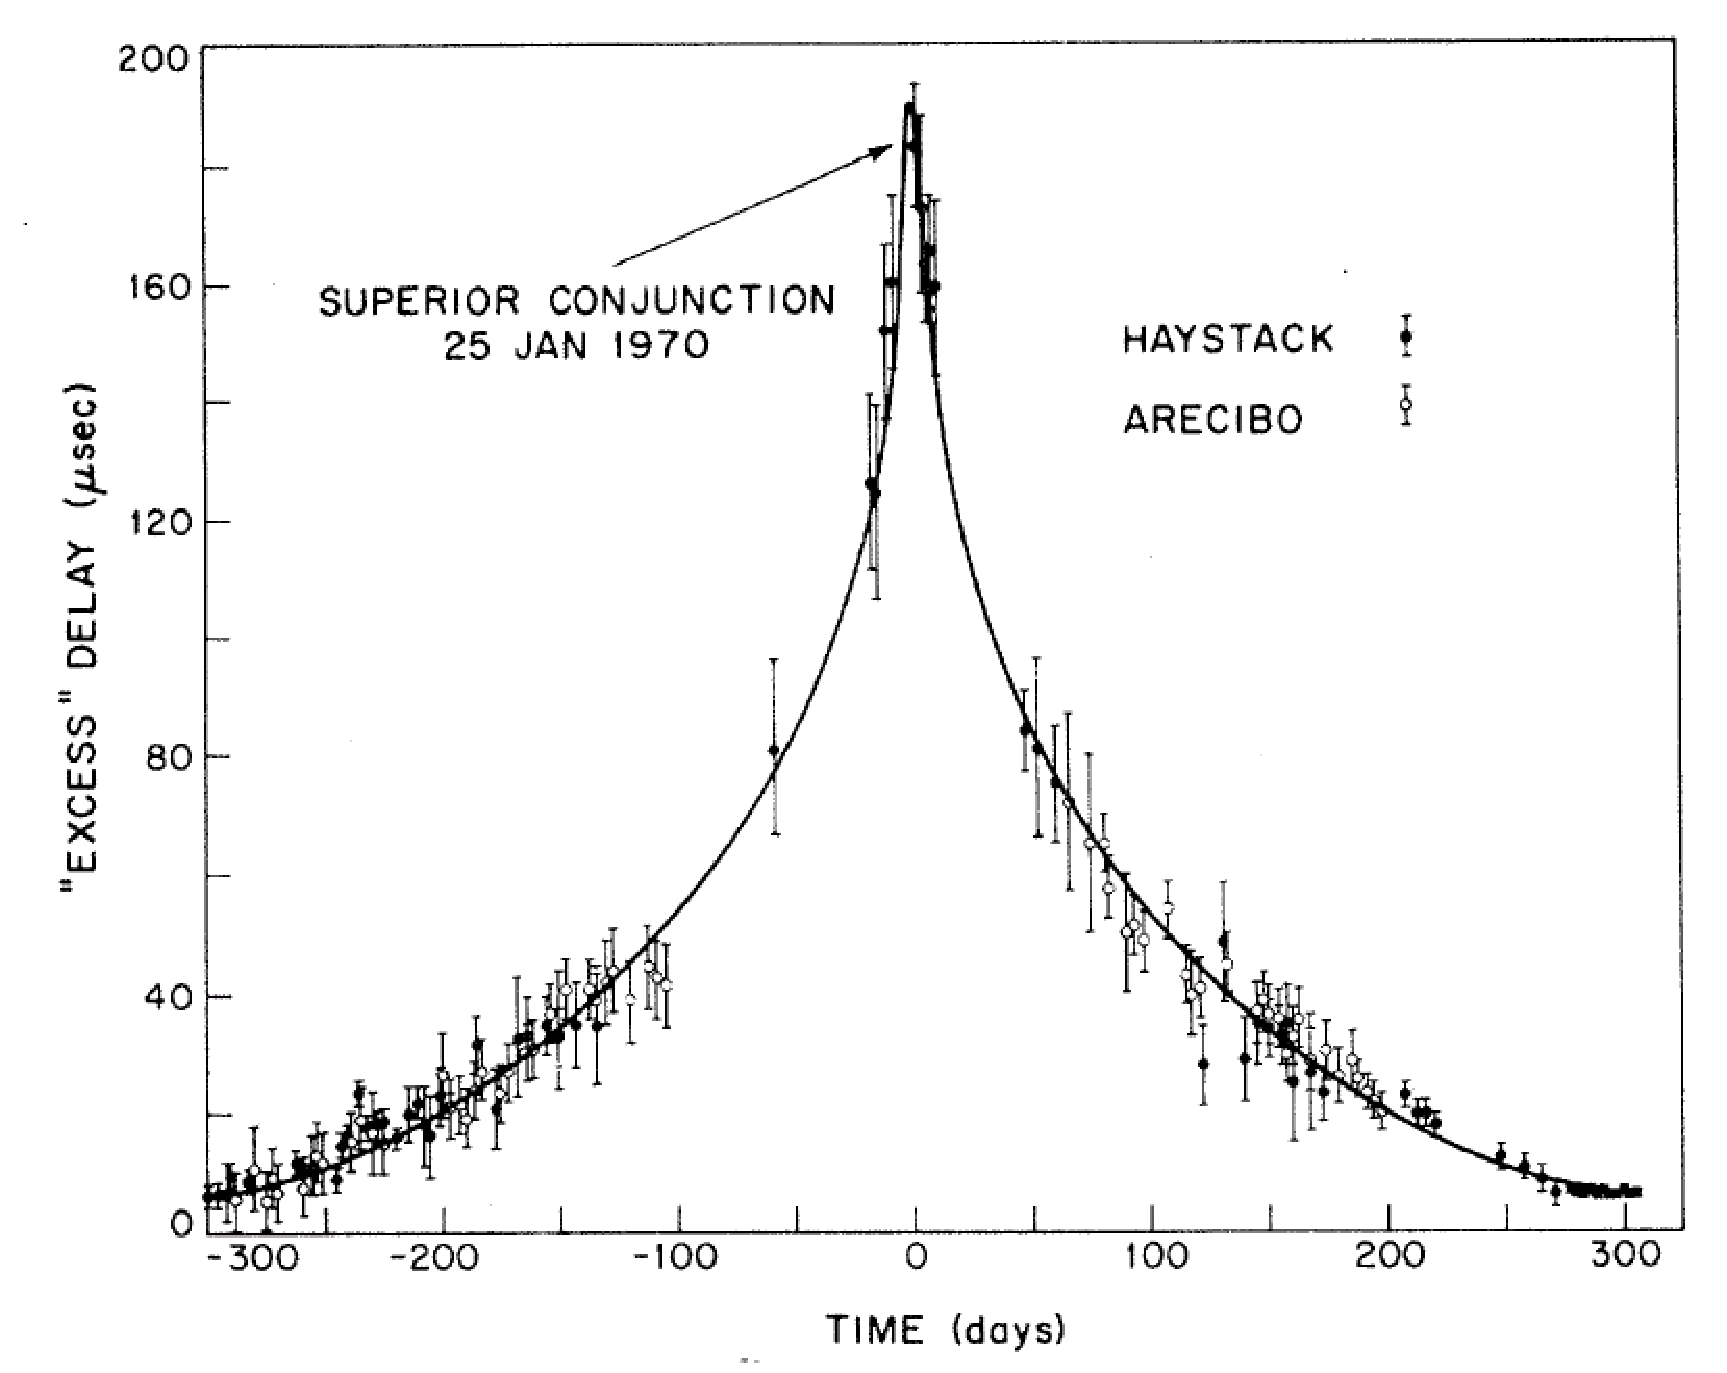
\includegraphics[height=6cm]{fig/fig-shapiro-delay-2.pdf}
\caption{Mediciones de Radar del efecto Shapiro.}
\end{center}
\end{figure}

\chapter{Agujeros Negros ***PRELIMINAR***}


\section{Singularidades y radio de Schwarzschild}

Aqu'i estudiaremos la estructura de la soluci'on de Schwarzschild en regiones \textit{cercanas al radio de Schwarzschild}, donde el campo gravitacional es muy intenso. En otras palabras, estudiaremos las geometr'ia del espaciotiempo esf'ericamente sim'etrico de una masa $M$ suficientemente compacta para que su tama\~no (la coordenada radial correspondiente a su superficie) sea menor que $2m$. Por ahora, postergaremos la importante discusi'on acerca de si existe un mecanismo f'isico realista para que una distribuci'on de masa pueda llegar a esta configuraci'on.

La geometr'ia del espaciotiempo de Schwarzschild, en coordenadas de
curvatura, es decir (\ref{Sch}), parece tener un mal comportamiento cerca de
$r=0$ y adem'as en $r=2m$, es decir, en el origen y en la esfera definida por
la condici'on que la coordenada radial $r$ sea igual al radio de Schwarzschild.
\begin{eqnarray}
 g_{00}&\to& -\infty,\quad g_{11}\to 0, \qquad \text{para}\quad r\to 0 ,\\
 g_{00}&\to& 0,\quad g_{11}\to -\infty, \qquad \text{para}\quad r\to 2m^+ .
\end{eqnarray}
Los coeficientes m'etricos son cantidades dependientes de las coordenadas
usadas, por lo que sus valores no necesariamente est'an relacionados con
cantidades f'isicas singulares. Para saber si estos comportamientos
singulares/divergentes son f'isicos, o s'olo \textit{singularidades coordenadas},
necesitamos considerar propiedades que sean independientes de las coordenadas
usadas.

Es relativamente f'acil generar singularidades coordenadas. Consideremos por ejemplo, el espacio euclidiano bidimensional $E_2$, con su elemento de l'inea en coordenadas cartesianas:
\begin{equation}
ds^2=dx^2+dy^2.
\end{equation}
Si introducimos una nueva coordenada $\xi$ por medio de
\begin{equation}
\xi:=\frac{1}{3}x^3,
\end{equation}
tendremos que la m'etrica toma la forma%
\begin{equation}
ds^2 =\left( 3\xi\right) ^{-\frac{4}{3}}d\xi^2+dy^2.
\end{equation}
La m'etrica parece tener ahora una singularidad en $\xi=0$. Sin embargo, esta
singularidad es totalmente removible introduciendo una ``nueva"\, variable $x$ por
medio de $\xi=x^3/3$. Por esto, se dice que 'esta es una
\textit{singularidad coordenada}. Es posible que tengamos una singularidad coordenada que sea el resultado de un quiebre de un sistema coordenado espec'ifico en lugar de ser una singularidad de la variedad subyacente. En otras palabras, se dice que la variedad tiene una singularidad (``verdadera'' o ``intr'inseca'') en su geometr'ia \textit{si ella no puede ser removida por un cambio de coordenadas apropiado}. En general no es obvio encontrar la manera de remover una singularidad coordenada.

Una forma de testear si una regi'on contiene singularidades de la geometr'ia (es decir, que no sean simples singularidades coordenadas) es calcular invariantes (es decir, escalares) a partir de contracciones del tensor de curvatura. Los escalares m'as simples son el escalar de curvatura
$R$, y sus contracciones $R_{\mu\nu\rho\sigma}R^{\mu\nu\rho\sigma}$, $R_{\mu\nu\rho\sigma}R^{\rho\sigma\lambda\tau}R^{\mu\nu}{}_{\lambda\tau}$, etc. Si alguno de estos escalares \textit{diverge} al acercarse a alg'un punto, tal punto es una singularidad de la geometr'ia. As'i, tenemos una condici'on \textit{suficiente}
para mostrar que un punto es una singularidad de la geometr'ia. Por otro lado, en general no es f'acil mostrar que un punto \textit{no es} singularidad.

En el caso de la m'etrica de Schwarzschild un c'alculo directo muestra que
\begin{equation}
R_{\mu\nu\rho\sigma}R^{\mu\nu\rho\sigma}=\frac{48m^2}{r^6},
\end{equation}
lo que prueba que $r=0$ (el origen del sistema coordenado usado) representa una
singularidad de la geometr'ia, donde la curvatura diverge. Puede verificarse que en $r=2m$ ninguno de los invariantes de curvatura arriba mencionados diverge. Por lo tanto, la esfera definida por $r=2m$ no es una singularidad de la curvatura (que mide propiedades locales de la variedad), sino algo diferente ...

\begin{itemize}
\item En $r=2m$, $g_{11}$ es infinito y $g_{00}$ es cero. Dado que $g_{00}
$ es cero, la superficie esf'erica en $r=2m$ es una \textit{superficie
infinitamente desplazada al rojo} por efecto de la dilataci'on temporal gravitacional. Ver la expresi'on (\ref{rgsch}). Decimos entonces que la superficie $r=2m$ es una \textit{superficie de redshift infinito}.

\item Adem'as, cuando $r<2m$, el signo de las componentes $g_{00}$ y $g_{11}$ cambian: $g_{00}$ se convierte en negativo y $g_{11}$ en positivo. Esto nos fuerza a reconsiderar el significado f'isico de $t$ y $r$. En efecto, en la regi'on del espaciotiempo con $r<2m$, $t$ es una coordenada tipo espacio y $r$ tipo tiempo, ya que una curva a lo largo del eje $t$ ($r$, $\theta$ y $\varphi$ constantes) posee $ds^2<0$, mientras que una curva a lo largo del eje $r$ ($t$, $\theta$ y $\varphi$ constantes) posee $ds^2>0$. Como veremos m'as adelante, esto trae como consecuencia que toda part'icula dentro de la regi'on delimitada por $r=2m$ caer'a hacia la singularidad central. Debido a esto, la superficie $r=2m$ es adicionalmente un \textit{horizonte de eventos}.
\end{itemize}

Estas caracter'isticas muestran que $r=2m$ es un radio inusual, pero
esto no implica que la geometr'ia local del espaciotiempo sea
singular en $r=2m$, como s'i ocurre en $r=0$.

Para analizar las propiedades f'isicas de la regi'on en torno a $r=2m$ con m'as detalle, estudiaremos las propiedades de fotones y de part'iculas en movimiento radial ``cayendo'' hacia (y ``escapando'' desde) la singularidad central.

\subsection{Diagrama Espacio-Temporal en Coordenadas de Schwarzschild}

Una manera de entender una geometr'ia es explorando su estructura causal, que est'a definida por las propiedades de propagaci'on de la luz. Consideremos en particular curvas (geod'esicas)
radiales tipo luz, es decir, para las cuales $\theta$ y $\varphi$ son constantes y
$ds^2=0$. Esta 'ultima condici'on se reduce a
\begin{equation}
 \left(1-\frac{2m}{r}\right) c^2dt^2-\frac{dr^2}{\left( 1-\frac
{2m}{r}\right) }=0,
\end{equation}
de donde obtenemos que
\begin{equation}
 c\frac{dt}{dr}=\pm\frac{1}{\left| 1-\frac{2m}{r}\right|}. \label{dtdr1}
\end{equation}
Considerando que
\begin{equation}
 \int_a^b\frac{dr}{\left| 1-\frac{2m}{r}\right|}=\pm\left[b-a+2m\ln\left(\frac{b-2m}{a-2m}\right)\right], \quad a<b,
\end{equation}
donde el signo positivo y negativo corresponde a los casos en que $a,b>2m$ y $a,b<2m$, respectivamente, podemos integrar (\ref{dtdr1}).

Si $r>2m$ el signo $+$ en (\ref{dtdr1}) corresponde a fotones alej'andose del centro de simetr'ia y el signo $-$ a fotones acerc'andose a 'este. En este caso obtenemos,
\begin{equation}
 c(t-t_0)=r-r_0+2m\ln\left(\frac{r-2m}{r_0-2m}\right),  \label{rtfs}
\end{equation}
para fotones salientes, y
\begin{equation}
 c(t-t_0)=r_0-r-2m\ln\left(\frac{r-2m}{r_0-2m}\right), \label{rtfe}
\end{equation}
para fotones entrantes, que pasan por el evento con coordenadas $(ct_0,r_0)$, respectivamente.
\begin{figure}[H]
 \begin{center}
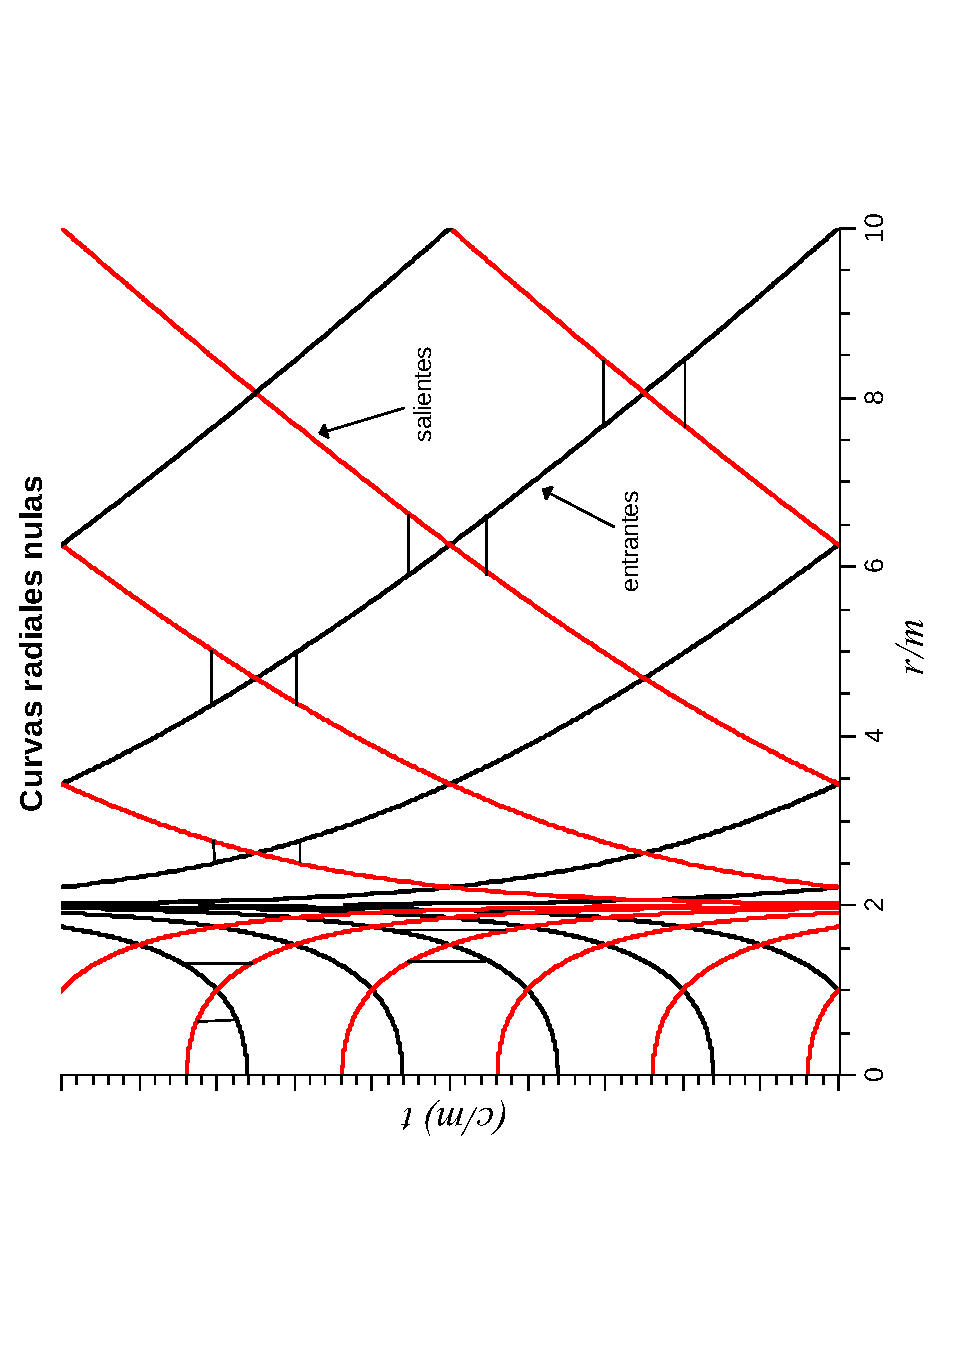
\includegraphics[height=8cm,angle=-90]{fig/fig-nullrays-cc-01.pdf}
\caption{Curvas nulas radiales en coordenadas de curvatura.}
\label{fig:nullrays-cc}
\end{center}
\end{figure}
Como es de esperar, muy lejos del centro de fuerzas $r\gg 2m$, recobramos
\begin{equation}
\frac{dr}{dt}=\pm\, c,
\end{equation}
tal como en un espaciotiempo plano. Por otro lado, cuando $r$ se aproxima a $2m$ (por ``la derecha'', es decir, con valores mayores a $2m$), tenemos
\begin{equation}
\frac{dt}{dr}\rightarrow\pm\infty,
\end{equation}
y los conos de luz se ``cierran", ya que las l'ineas tienden a ser
paralelas al eje $t$. Esto tendr'a como consecuencia que al acercarse a $r=2m$ la coordenada temporal de la trayectoria del fot'on aumentar'a indefinidamente. En otras palabras, en t'erminos de la coordenada temporal $t$, a medida que un rayo de luz se aproxima a $r=2m$ pareciera que el fot'on nunca llegar'a all'i. En realidad, como veremos a continuaci'on, un rayo de luz no tiene problemas en alcanzar $r=2m$ (tampoco part'iculas masivas), pero un observador lejos de $r=2m$ nunca ser'ia capaz de ``ver'' este hecho.

En efecto, para describir c'omo se ``ve''\, la ca'ida del fot'on desde lejos, consideraremos un observador en reposo en $r=R>2m$ y c'omo 'este puede informarse sobre la ca'ida del fot'on.

Para esto, consideramos un fot'on cayendo hacia la singularidad, y dos eventos $E_1$ y $E_2$ en su l'inea de mundo, con coordenadas $(ct,r)=(ct_1,r_1)$ y $(ct,r)=(ct_2,r_2)$ respectivamente, con $r_2<r_1<R$. De acuerdo a lo anterior, las coordenadas de estos eventos est'an relacionadas por medio de
\begin{equation}
c(t_2-t_1)=r_1-r_2+2m\ln\left(\frac{r_1-2m}{r_2-2m}\right). \label{t2t1}
\end{equation}
Consideremos que cuando el fot'on pasa por el evento $E_1$ una se~nal luminosa (otro fot'on) es enviada hacia el observador en $R>r_1$. Este nuevo fot'on viaja desde el evento $E_1$ hasta el evento de recepci'on $R_1$, con coordenadas $(ct,r)=(ct_{1\rm r},R)$. Como estos eventos pertenecen a la l'inea de mundo de un fot'on alej'andose de la singularidad, sus coordenadas satisfacen
\begin{equation}
c(t_{1 \rm r}-t_1)=R-r_1+2m\ln\left(\frac{R-2m}{r_1-2m}\right).\label{t1rt1}
\end{equation}
Similarmente, si en el evento $E_2$ se emite una segunda se\~nal luminosa hasta el observador, de modo que 'este la recibe en el evento $R_2$ con coordenadas $(ct,r)=(ct_{2\rm r},R)$, entonces
\begin{equation}
c(t_{2 \rm r}-t_2)=R-r_2+2m\ln\left(\frac{R-2m}{r_2-2m}\right).\label{t2rt2}
\end{equation}
El intervalo de coordenada temporal entre la recepci'on de las dos se~nales por el observador en reposo en la posici'on $r=R$ es dada por $(\Delta t)_{\rm r}=t_{2 \rm r}-t_{1 \rm r}$. Usando (\ref{t2t1}), (\ref{t1rt1}) y (\ref{t2rt2}), encontramos
\begin{equation}
c(\Delta t)_{\rm r}=2\left[r_1-r_2+2m\ln\left(\frac{r_1-2m}{r_2-2m}\right)\right].
\end{equation}
En otras palabras, $(\Delta t)_{\rm r}=2(t_2-t_1)$. Finalmente, el tiempo (propio) medido por el observador en $r=R$ entre las dos se~nales es $(\Delta\tau)_{\rm r}=(\Delta t)_{\rm r}\sqrt{1-2m/R}$. En particular, para un observador ``en el infinito", tendremos simplemente que
$(\Delta\tau)_{{\rm r},\infty}=2(t_2-t_1)$. Como consecuencia, desde el punto de vista de un observador externo (en $r=R$, o en el infinito) el fot'on requiere un tiempo infinito en llegar a $r=2m$, es decir, \textit{el observador nunca registra que el fot'on cruza el horizonte}, sino que lo observa acercarse cada vez m'as lentamente. No obtante, como veremos a continuaci'on, el fot'on no encuentra ning'un obst'aculo al acercarse al horizonte, cruz'andolo y alcanzando finalmente la singularidad central.

\subsection{Coordenadas de Eddington-Finkelstein}

Hemos visto que en t'erminos de las coordenadas de curvatura los conos de luz parecen comprimirse a medida que se acercan a $r=2m$, y que las curvas tipo luz radiales entrantes parecen nunca cruzar el horizonte, ya que estas curvas se tornan cada vez m'as verticales.

Es posible introducir nuevas coordenadas en las que estas caracter'isticas no est'an presentes. Espec'ificamente, podemos elegir nuevas coordenadas $\bar{x}^\mu=(c\bar{t},r,\theta,\varphi)$, en las que las l'ineas nulas radiales entrantes sean rectas con un 'angulo de 45 grados respecto al eje $r$. De (\ref{rtfe}) vemos que si definimos la \textit{coordenada de Eddington-Finkelstein retardada} por
\begin{equation}
 \bar{t}(t,r):=t+\frac{2m}{c}\ln\left|r-2m\right|, \label{tEF}
\end{equation}
entonces la relaci'on que define la trayectoria de un fot'on entrante es simplemente
\begin{equation}
 c(\bar{t}-\bar{t}_0)=r_0-r,
\end{equation}
que en el plano $(c\bar{t},r)$  corresponde precisamente una l'inea recta con pendiente $-1$.

En t'erminos de las nuevas coordenadas $\bar{x}^\mu$ el elemento de l'inea adopta la forma siguiente:
\begin{equation}\marginnote{Schwarzschild, Eddington-Finkelstein}
 ds^2=\left(1-\frac{2m}{r}\right)c^2d\bar{t}^2-\frac{4m}{r}c\,d\bar{t}\,dr-\left(1+\frac{2m}{r}\right)dr^2-r^2\left(d\theta^2+\sen^2\theta\,d\varphi^2\right). \label{dsEF}
\end{equation}
Vemos que la m'etrica en estas coordenadas es regular en $r=2m$. De hecho, ella es regular en todo el rango $0<r<2m$. Puede argumentarse que la transformaci'on (\ref{tEF}) no es v'alida para puntos con $r\le 2m$ y que por consiguiente (\ref{dsEF}) s'olo ser'ia v'alida en la regi'on fuera del horizonte. Sin embargo, en la teor'ia de RG, la m'etrica de Schwarzschild en coordenadas de curvatura, con $0<r<\infty$ es una soluci'on tan leg'itima de las ecuaciones de Einstein en el vac'io como lo es la m'etrica asociada a (\ref{dsEF}) con $0<r<\infty$. En general, el criterio usado es que, dada una m'etrica que es soluci'on de las Ecuaciones de Einstein, se busca el rango m'aximo de variaci'on de las coordenadas tales que la soluci'on sea v'alida. En otras palabras, puede perfectamente considerarse la m'etrica en coordenadas de Eddington-Finkelstein como la ``m'etrica original'', v'alida en todo el rango $0<r<\infty$, y la m'etrica en coordenadas de curvatura como s'olo apropiada en la regi'on exterior al horizonte. En cierto sentido, la m'etrica en coordenadas Eddington-Finkelstein es una suerte de ``continuaci'on anal'itica'' de la m'etrica de la soluci'on en coordenadas de curvatura.

Como vimos, en coordenadas de Eddington-Finkelstein, las l'ineas nulas radiales entrantes son l'ineas rectas. Por otro lado, las curvas nulas radiales \textit{salientes} est'an descritas por la relaci'on
\begin{equation}
 c(\bar{t}-\bar{t}_0)=r-r_0+4m\ln\left|\frac{r-2m}{r_0-2m}\right|,  \label{rtfsEF}
\end{equation}
que se obtiene directamente de (\ref{rtfs}) y la definici'on (\ref{tEF}).

\begin{figure}[H]
 \begin{center}
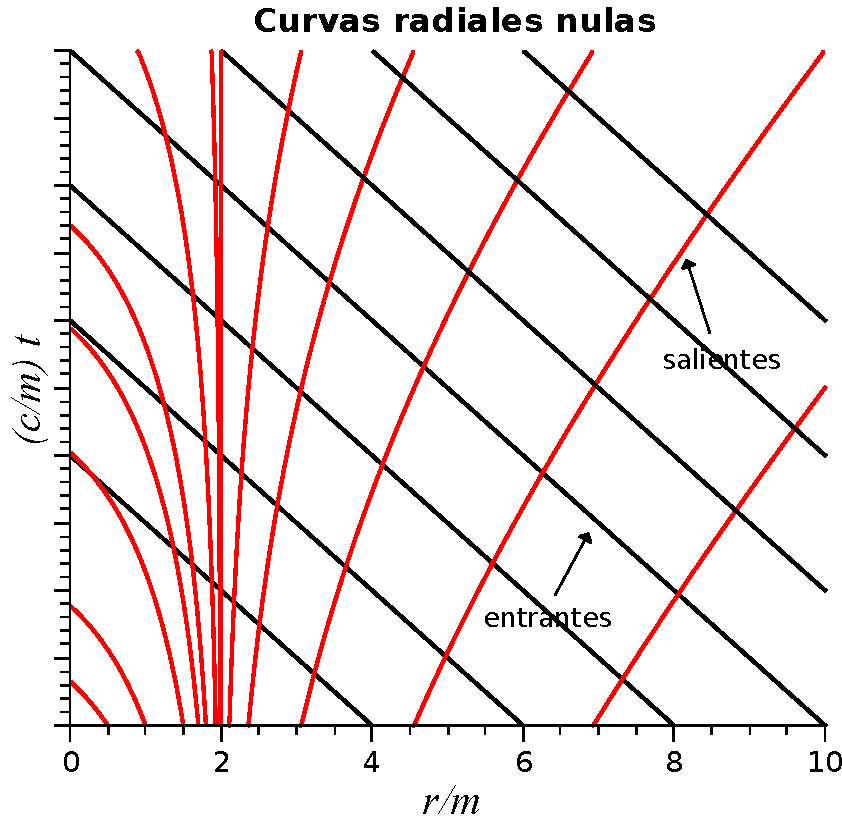
\includegraphics[height=6cm]{fig/fig-nullrays-cEF-2.pdf}
\caption{Curvas nulas radiales en coordenadas de Eddington-Finkelstein.}
\label{fig:nullrays-cEF}
\end{center}
\end{figure}

Vemos que la superficie definida por $r=2m$ act'ua como una ``membrana unidireccional'', en el sentido que s'olo permite cruzar a part'iculas cayendo hacia la singularidad central. Las l'ineas de mundo entrantes cruzan desde la regi'on externa hacia la interna. La superficie $r=2m$ es llamada un \textit{horizonte de eventos} ya que representa la regi'on que delimita los eventos que pueden ser en principio observados por un observador externo. El horizonte de Schwarzschild es \textit{absoluto} en el sentido que impide \textit{a todo observador externo} obtener informaci'on de eventos dentro del horizonte.

\subsection{Part'iculas cayendo radialmente}

Consideremos la trayectoria de una part'icula cayendo libremente en un movimiento radial hacia la singularidad. La trayectoria es entonces una geod'esica radial tipo tiempo. De acuerdo a lo estudiado anteriormente, en este caso la trayectoria tiene como constantes de movimiento a $k$ y $h$ dadas por (\ref{kh}), con $h=0$. De entre las posibles trayectorias, deteminadas por la constante $k$, nos concentraremos en aquellas correspondientes a part'iculas que caen  ``desde el reposo en el infinito'', es decir, tal que $\dot{r}\to 0$ para $r\to\infty$. En este caso la relaci'on (\ref{uuc22}) implica que $k^2=1$. Finalmente, (\ref{kh}a), muestra que para trayectorias ``orientadas hacia el futuro'', $k=1$. Con esto, (\ref{uuc22}) se reduce en este caso a
\begin{equation}
\dot{r}^2 =\frac{2mc^2}{r} .\label{pi1}
\end{equation}
Como estamos considerando una part'icula acerc'andose a la singularidad central, tendremos entonces que
\begin{equation}
\frac{dr}{d\tau}=-c\sqrt{\frac{2m}{r}} .
\end{equation}
Podemos integrar esta expresi'on directamente, y obtenemos
\begin{equation}
 c(\tau-\tau_0)=\frac{2}{3\sqrt{2m}}\left(r_0^{3/2}-r^{3/2}\right), \label{taurclr}
\end{equation}
donde $\tau_0$ es el tiempo propio (del reloj com'ovil con la part'icula) registrado en el instante en que 'esta pasa por $r=r_0$. Note que la expresi'on encontrada, (\ref{taurclr}), es la misma que el caso newtoniano. Como consecuencia, el intervalo de tiempo propio desde que la part'icula cruza $r=r_0$ y que llega a la singularidad central es finito:
\begin{equation}
 c(\tau|_{r=0}-\tau_0)=\frac{2}{3\sqrt{2m}}r_0^{3/2}.
\end{equation}
En particular, el tiempo propio requerido para caer desde el horizonte hasta la singularidad central es $4m/3c$

Para analizar c'omo var'ia la coordenada $t$ en este proceso, podemos escribir
\begin{equation}
 c\frac{dt}{dr}=c\frac{\dot{t}}{\dot{r}}=-\frac{1}{1-\frac{2m}{r}}\sqrt{\frac{r}{2m}}.
\end{equation}
Integrando esta expresi'on\footnote{$\int\sqrt{\frac{r}{a}}\frac{dr}{1-\frac{a}{r}}=\frac{2}{3}a\, (r/a)^{3/2}+2a\,(r/a)^{1/2}-a\ln\left(\frac{\sqrt{r}-\sqrt{a}}{\sqrt{r}+\sqrt{a}}\right) $.} encontramos
\begin{equation}
c(t-t_0)=-\frac{2}{3\sqrt{2m}}\left(r^{3/2} -r_0^{3/2}+6m\sqrt{r}-6m\sqrt{r_0}\right)+2m\ln\left[\frac{(\sqrt{r}+\sqrt{2m})(\sqrt{r_0}-\sqrt{2m})}{(\sqrt{r}-\sqrt{2m})(\sqrt{r_0}+\sqrt{2m})}\right].
\end{equation}
Vemos de esta expresi'on que la coordenada temporal de la trayectoria de la part'icula crece indefinidamente a medida que 'esta se acerca al horizonte.

% \section{Coordenadas de Eddington-Finkelstein}
%
% \begin{align}
% \left[ \left( 1-\frac{2m}{r}\right) \frac{2m^2}{\left(
% r-2m\right) ^2}-\frac{1}{\left( 1-\frac{2m}{r}\right) }\right]
% dr^2 & =\left[ \frac{2m^2}{r\left( r-2m\right) }-\frac
% {1}{\left( 1-\frac{2m}{r}\right) }\right] dr^2\\
% & =\left[ \frac{\left( 1-\frac{2m}{r}\right) 2m^2-r\left(
% r-2m\right) }{r\left( r-2m\right) \left( 1-\frac{2m}{r}\right)
% }\right] dr^2\\
% & =\left[ \frac{2m^2-r^2}{r\left( r-2m\right) }\right] dr^2\\
% & =\left[ \frac{\left( 2m-r\right) \left( 2m+r\right) }{r\left(
% r-2m\right) }\right] dr^2\\
% & =-\left[ \frac{\left( r-2m\right) \left( 2m+r\right) }{r\left(
% r-2m\right) }\right] dr^2\\
% & =-\left[ \frac{\left( 2m+r\right) }{r}\right] dr^2=-\left[
% 1+\frac{2m}{r}\right] dr^2%
% \end{align}
% de manera que%
% \begin{equation}
% ds^2=\left( 1-\frac{2m}{r}\right) d\overline{t}^2-\frac{22m}%
% {r}d\overline{t}dr-\left( 1+\frac{2m}{r}\right) dr^2-r^2d\Omega
% ^2\label{ef9}%
% \end{equation}
% expresi'on conocida como la forma de Eddington-Finkelstein de la
% m'etrica de Schwarzchild. Notemos que la soluci'on es ahora regular en
% $r=2m$, adem'as es tambi'en regular para todo el rango $\left(
% 0<r<2m\right) $. De modo que en alg'un sentido, la transformaci'on
% dada por la Ec. (\ref{ef6}) extiende el rango de las
% coordenadas desde $2m<r<\infty$ a $0<r<\infty$. El proceso es alguna
% reminiscencia de una continiaci'on anal'itica de una funci'on en
% an'alisis complejo. Debido a esto Ec. (\ref{ef9}) es llamada
% la extensi'on anal'itica de la soluci'on de Schwarzschild.
% Podr'ia ser objetado que la transformaci'on de coordenadas dada por
% Ec. (\ref{ef5}) no puede ser usada en $r=2m$ debido a que
% ella se convierte en singular. Sin embargo, Ec. (\ref{ef5}) es
% una herramienta conveniente para ir desde la soluci'on de Schwarzschild a
% Ec. (\ref{ef9}). Nuestro punto de partida es en realidad en
% base a estos dos elementos de l'inea. Dadas estas soluciones, la pregunta
% es \textquestiondown Cu'al es el mayor rango de las coordenadas para las
% cuales cada soluci'on es regular?. La respuesta es $2m<r<\infty$ para la
% soluci'on de Schwarzschild y $0<r<\infty$ para la forma de
% Eddington-Finkelstein (junto, obviamente a $-\infty<t<\infty,$ $0\leq
% \theta\leq\pi$ y $-\pi\leq\varphi\leq\pi$). En la regi'on de traslape
% ($2m<r<\infty$), las dos soluciones est'an relacionadas por medio de la
% transformaci'on \ref{ef5} y por lo tanto, ellas representan la misma
% soluci'on en esta regi'on.
%
% Notemos que la soluci'on en las coordenadas de Eddington-Finkelstein no es
% sim'etrica en el tiempo. Podemos obtener una soluci'on con el tiempo
% inverso introduciendo, en lugar de Ec. (\ref{ef6}), la
% siguiente transformaci'on en la coordenada temporal%
% \begin{equation}
% t\rightarrow\overline{t}=t-2m\ln\left( \frac{2m}{r}-1\right)
% \label{ef10}%
% \end{equation}
% para $r>2m$. Esto implica que la congruencia \ref{ef4} toma la forma
% \begin{align}
% t & =r+2m\ln\left( \frac{r}{2m}-1\right) +cte\nonumber\\
% \overline{t}+2m\ln\left( \frac{2m}{r}-1\right)  & =r+2m\ln\left(
% \frac{r}{2m}-1\right) +cte\nonumber\\
% \overline{t} & =r+cte\label{ef11}%
% \end{align}
% la cual es una l'inea que forma un 'angulo de $45^{\circ}$ con el eje
% $r$. De Ec. (\ref{ef10}) vemos que
% \begin{equation}
% d\overline{t}=dt-2m\frac{1}{\frac{r}{2m}-1}d\left( \frac{r}{2m%
% }\right) =dt-\frac{1}{\frac{r-2m}{2m}}dr=dt-\frac{2m}{r-2m}dr
% \end{equation}
% $\Longrightarrow$%
% \begin{equation}
% dt=d\overline{t}+\frac{2m}{r-2m}dr\label{ef12}%
% \end{equation}
%
%
% Introduciendo Ec. (\ref{ef12}) en la soluci'on de Schwarzschild tenemos%
% \begin{align}
% ds^2 & =\left( 1-\frac{2m}{r}\right) dt^2-\frac{dr^2}{\left(
% 1-\frac{2m}{r}\right) }-r^2d\Omega^2\nonumber\\
% ds^2 & =\left( 1-\frac{2m}{r}\right) \left( d\overline{t}+\frac
% {2m}{r-2m}dr\right) ^2-\frac{dr^2}{\left( 1-\frac{2m}%
% {r}\right) }-r^2d\Omega^2\nonumber\\
% ds^2 & =\left( 1-\frac{2m}{r}\right) \left( d\overline{t}^2%
% +2\frac{2m}{r-2m}d\overline{t}dr+\frac{2m^2}{\left( r-2m%
% \right) ^2}dr^2\right) -\frac{dr^2}{\left( 1-\frac{2m}{r}\right)
% }-r^2d\Omega^2\nonumber\\
% ds^2 & =\left( 1-\frac{2m}{r}\right) \left( d\overline{t}^2%
% +2\frac{2m}{r-2m}d\overline{t}dr+\frac{2m^2}{\left( r-2m%
% \right) ^2}dr^2\right) -\frac{dr^2}{\left( 1-\frac{2m}{r}\right)
% }-r^2d\Omega^2\nonumber\\
% ds^2 & =\left( 1-\frac{2m}{r}\right) d\overline{t}^2+2\left(
% 1-\frac{2m}{r}\right) \frac{2m}{r-2m}d\overline{t}dr+\left(
% 1-\frac{2m}{r}\right) \frac{2m^2}{\left( r-2m\right) ^2}%
% dr^2-\frac{dr^2}{\left( 1-\frac{2m}{r}\right) }-r^2d\Omega
% ^2\nonumber\\
% ds^2 & =\left( 1-\frac{2m}{r}\right) d\overline{t}^2+2\left(
% \frac{r-2m}{r}\right) \frac{2m}{r-2m}d\overline{t}dr+\left(
% \frac{r-2m}{r}\right) \frac{2m^2}{\left( r-2m\right) ^2}%
% dr^2-\frac{rdr^2}{\left( r-2m\right) }-r^2d\Omega^2\nonumber\\
% ds^2 & =\left( 1-\frac{2m}{r}\right) d\overline{t}^2+2\frac{2m%
% }{r}d\overline{t}dr+\left[ \left( \frac{r-2m}{r}\right) \frac{2m^2%
% }{\left( r-2m\right) ^2}-\frac{r}{\left( r-2m\right) }\right]
% dr^2-r^2d\Omega^2\nonumber\\
% ds^2 & =\left( 1-\frac{2m}{r}\right) d\overline{t}^2+2\frac{2m%
% }{r}d\overline{t}dr+\left[ \frac{2m^2}{r\left( r-2m\right) }%
% -\frac{r}{\left( r-2m\right) }\right] dr^2-r^2d\Omega^2\nonumber\\
% ds^2 & =\left( 1-\frac{2m}{r}\right) d\overline{t}^2+2\frac{2m%
% }{r}d\overline{t}dr+\left[ \frac{2m^2-r^2}{r\left( r-2m\right)
% }\right] dr^2-r^2d\Omega^2\nonumber\\
% ds^2 & =\left( 1-\frac{2m}{r}\right) d\overline{t}^2+2\frac{2m%
% }{r}d\overline{t}dr+\left[ \frac{\left( 2m-r\right) \left(
% 2m+r\right) }{r\left( r-2m\right) }\right] dr^2-r^2d\Omega
% ^2\nonumber\\
% ds^2 & =\left( 1-\frac{2m}{r}\right) d\overline{t}^2+2\frac{2m%
% }{r}d\overline{t}dr-\left( 1+\frac{2m}{r}\right) dr^2-r^2d\Omega
% ^2\label{ef13}%
% \end{align}
% expresi'on conocida como la m'etrica de Schwarzchild en coordenadas de
% Eddington-Finkelstein. As'i, la expresi'on más general para la
% m'etrica de Schwarzschild en las coordenadas de Eddington-Finkelstein viene
% dada por%
% \begin{equation}
% ds^2=\left( 1-\frac{2m}{r}\right) d\overline{t}^2\pm2\frac{2m}%
% {r}d\overline{t}dr-\left( 1+\frac{2m}{r}\right) dr^2-r^2d\Omega
% ^2\label{ef14}%
% \end{equation}
% Esta forma de la m'etrica es de nuevo independiente del tiempo pero no es
% diagonal. La m'etrica es ahora no singular en $r=2m$ y satisface las
% ecuaciones de campo de Einstein para todo valor $r>0$. Notemos sin embargo,
% que es requerida una transformaci'on singular para obtener este resultado.
%
% Mostremos ahora que las regiones a ambos lados de la superficie $r=2m$ se
% unen en forma suave sobre esta superficie. Un detallado entendimiento de la
% situaci'on se obtiene examinando la estructura general de los conos de luz
% de la m'etrica dada por Ec. (\ref{ef14}) en el plano
% $\left( \overline{t},r\right) $. Consideremos primero el caso del signo
% $\left( -\right) $.\ En este caso las direcciones radiales nulas ,con
% $\theta$ y $\varphi$ constantes, ser'an determinadas por la ecuaci'on%
% \begin{align}
% & ds^2=\left( 1-\frac{2m}{r}\right) d\overline{t}^2-2\frac{2m}%
% {r}d\overline{t}dr-\left( 1+\frac{2m}{r}\right) dr^2=0\nonumber\\
% & d\overline{t}^2-\frac{2m}{r}d\overline{t}^2-2\frac{2m}%
% {r}d\overline{t}dr-dr^2+\frac{2m}{r}dr^2=0\nonumber\\
% & d\overline{t}^2-dr^2-\frac{2m}{r}\left( d\overline{t}^2%
% +2d\overline{t}dr+dr^2\right) =0\nonumber\\
% & d\overline{t}^2-dr^2-\frac{2m}{r}\left( d\overline{t}+dr\right)
% ^2=0\nonumber\\
% & \left( d\overline{t}-dr\right) \left( d\overline{t}+dr\right)
% -\frac{2m}{r}\left( d\overline{t}+dr\right) ^2=0\nonumber\\
% & \left( d\overline{t}+dr\right) \left[ \left( d\overline{t}-dr\right)
% -\frac{2m}{r}\left( d\overline{t}+dr\right) \right] =0\nonumber\\
% & \left( d\overline{t}+dr\right) \left[ d\overline{t}-dr-\frac{2m}%
% {r}d\overline{t}-\frac{2m}{r}dr\right] =0\nonumber\\
% & \left( d\overline{t}+dr\right) \left[ \left( 1-\frac{2m}{r}\right)
% d\overline{t}-\left( 1+\frac{2m}{r}\right) dr\right] =0\label{ef15}%
% \end{align}
% de donde vemos que las direcciones nulas vienen dadas por%
% \begin{align}
% d\overline{t}+dr & =0\Longrightarrow\frac{dr}{d\overline{t}}=-1\label{ef16}\\
% \left( 1-\frac{2m}{r}\right) d\overline{t}-\left( 1+\frac{2m}%
% {r}\right) dr & =0\Longrightarrow\frac{dr}{d\overline{t}}=\frac{r-2m%
% }{r+2m}\label{ef17}%
% \end{align}
%
%
% Las l'ineas que son tangentes a una u otra de las direcciones dadas por
% Ec. (\ref{ef16}), (\ref{ef17}) son geod'esicas radiales nulas.
% De Ec. (\ref{ef16}) vemos que la primera familia de geod'esicas nulas posee la
% ecuaci'on%
% \begin{equation}
% d\left( \overline{t}+r\right) =0\Longrightarrow\overline{t}%
% +r=cte\label{ef18}%
% \end{equation}
% estas son l'ineas geod'esicas paralelas. La Ec. (\ref{ef17}) posee una
% integral menos simple. De ella vemos que
% \begin{align}
% \frac{dr}{d\overline{t}} & \rightarrow1\text{ para }r\rightarrow\infty\\
% \frac{dr}{d\overline{t}} & \rightarrow-1\text{ para }r\rightarrow0\\
% \frac{dr}{d\overline{t}} & \rightarrow0\text{ para }r\rightarrow 2m%
% \end{align}
%
%
% De la tercera de estas propiedades vemos que estas geod'esicas no cruzan la
% superficie $r=2m$ y ser'an de la forma mostrada en la figura.
%
% Es de inter'es recordar que las part'iculas se mueven sobre l'ineas
% de universo tipo tiempo o sobre l'ineas de universo nulas, es decir, sobre
% l'ineas que yacen en el interior o en la superficie del cono de luz. De la
% figura vemos que para $r>2m$ ninguna part'icula puede atravesar la
% hipersfera $r=2m$. Adem'as cualquier part'icula que en alg'un
% momento est'a en el interior de la superficie $r=2m$, se mover'a
% necesariamente hacia $r=0$ alcanzando esta l'inea en un tiempo finito, sea
% este coordenado o propio.
%
% El hecho de que ninguna part'icula, que en alg'un momento est'a en
% el interior de la superficie, pueda atravesar la superficie $r=2m$,
% significa que un observador $P$ situado en la regi'on $r>2m$ no puede
% recibir ninguna informaci'on acerca de eventos que ocurren al interior de
% la superficie $r=r_{0.}$ Por esto decimos que la hipersuperficie $r=2m$ es
% un horizonte de eventos para todos los observadores ubicados en la regi'on
% \thinspace$r>2m.$
%
% Consideremos ahora el caso del signo $\left( +\right) $. Las direcciones
% radiales nulas manteniendo $\theta,\varphi$ constantes son determinadas por
% \begin{align}
% & ds^2=\left( 1-\frac{2m}{r}\right) d\overline{t}^2+2\frac{2m}%
% {r}d\overline{t}dr-\left( 1+\frac{2m}{r}\right) dr^2=0\\
% & d\overline{t}^2-\frac{2m}{r}d\overline{t}^2+2\frac{2m}%
% {r}d\overline{t}dr-dr^2-\frac{2m}{r}dr^2=0\\
% & d\overline{t}^2-dr^2-\frac{2m}{r}\left( d\overline{t}^2%
% -2d\overline{t}dr+dr^2\right) =0\\
% & \left( d\overline{t}-dr\right) \left( d\overline{t}+dr\right)
% -\frac{2m}{r}\left( d\overline{t}-dr\right) ^2=0\\
% & \left( d\overline{t}-dr\right) \left[ \left( d\overline{t}+dr\right)
% -\frac{2m}{r}\left( d\overline{t}-dr\right) \right] =0\\
% & \left( d\overline{t}-dr\right) \left[ \left( 1-\frac{2m}{r}\right)
% d\overline{t}+\left( 1+\frac{2m}{r}\right) dr\right] =0
% \end{align}
% de donde vamos que las direcciones radiales nulas vienen dadas por%
% \begin{equation}
% d\overline{t}-dr=0\Longrightarrow\frac{dr}{d\overline{t}}=1\Longrightarrow
% \overline{t}-r=cte
% \end{equation}
% las cuales son rectas paralelas que forman un 'angulo de $45^{\circ}$ con
% el eje $r$. De aqui vemos que las part'iculas no tienen problemas para
% "salir" desde $r=0$ y atravesar la hipersuperficie $r=2m$. Por otra parte%
% \begin{align}
% & \left( 1-\frac{2m}{r}\right) d\overline{t}+\left( 1+\frac{2m}%
% {r}\right) dr=0\\
% & \frac{dr}{d\overline{t}}=-\frac{\left( 1-\frac{2m}{r}\right) }{\left(
% 1+\frac{2m}{r}\right) }\\
% & \frac{dr}{d\overline{t}}=-\frac{\left( r-2m\right) }{\left(
% r+2m\right) }%
% \end{align}
% de donde vemos que esta segunda familia tiene las siguientes propiedades:%
%
% \begin{align}
% \frac{dr}{d\overline{t}} & \rightarrow-1\ \text{\ para }%
% r\rightarrow\infty\nonumber\\
% \frac{dr}{d\overline{t}} & \rightarrow1\ \text{\ para }%
% r\rightarrow0\nonumber\\
% \frac{dr}{d\overline{t}} & \rightarrow0\text{ \ para }r\rightarrow
% 2m\label{efx1}%
% \end{align}
% al igual que en el caso anterior, ec. (\ref{efx1}) indica que
% estas familias de goed'esicas nulas nunca atraviesan la superficie
% $r=2m$ y al contrario del caso anterior, cualquier part'icula que se
% mueva al interior de $r=2m$, se mover'a asint'oticamente hacia
% $r=2m$ y nunca tocar'a la singularidad $r=0.$Para un observador ubicado
% en la regi'on $r>2m$ vemos que este tambi'en se mueve
% asint'oticamente a la hipersuperficie $r=2m$. De esta forma vemos que
% los eventos en las regiones $r>2m$ y $r<2m$ est'an desconectados, por
% lo tanto, $r=2m$ sigue siendo un horizonte de eventos.




% \section{Coordenadas de Kruskal}
%
% Kruskal introdujo un sistema coordenado esf'ericamente sim'etrico en el
% cual los rayos de luz radial tienen en todas partes la pendiente $\frac
% {dr}{dt}=\pm1$. Consideremos la soluci'on a la ecuaci'on
% \begin{equation}
% \frac{dt}{dr}=\pm\left( 1-\frac{2m}{r}\right) ^{-1}%
% \end{equation}
% la cual es dada por%
% \begin{equation}
% t=\pm r^{\ast}+cte=\pm\left[ r+2m\ln\left( \frac{r}{2m}-1\right)
% \right] +cte
% \end{equation}
% las coordenadas de Eddington-Finkelstein se obtienen haciendo%
% \begin{equation}
% t\rightarrow\overline{t}_{\pm}=t\pm 2m\ln\left( \frac{2m}{r}-1\right)
% \text{, para }r>2m%
% \end{equation}
% en las cuales%
% \begin{equation}
% ds^2=\left( 1-\frac{2m}{r}\right) d\overline{t}_{\pm}^2\pm
% 2\frac{2m}{r}d\overline{t_{\pm}}dr-\left( 1+\frac{2m}{r}\right)
% dr^2-r^2d\Omega^2\label{ck1}%
% \end{equation}
% la Ec. (\ref{ck1}) puede ser escrita de una manera más simple introduciendo
% una coordenada nula
% \begin{equation}
% v=\overline{t}_{+}+r\label{ck2}%
% \end{equation}
% conocida como \textit{par'ametro de tiempo avanzado}$.$%
% \begin{align}
% dv & =d\overline{t}_{+}+dr\\
% d\overline{t}_{+} & =dv-dr\\
% d\overline{t}_{+}^2 & =dv^2-2dvdr+dr^2%
% \end{align}
% $\Longrightarrow$%
% \begin{align}
% ds^2 & =\left( 1-\frac{2m}{r}\right) d\overline{t_{+}}^2%
% -2\frac{2m}{r}d\overline{t_{+}}dr-\left( 1+\frac{2m}{r}\right)
% dr^2-r^2d\Omega^2\nonumber\\
% ds^2 & =\left( 1-\frac{2m}{r}\right) \left( dv^2-2dvdr+dr^2%
% \right) -2\frac{2m}{r}\left( dv-dr\right) dr-\left( 1+\frac{2m}%
% {r}\right) dr^2-r^2d\Omega^2\nonumber\\
% ds^2 & =\left( 1-\frac{2m}{r}\right) dv^2-2\left( 1-\frac{2m}%
% {r}\right) dvdr+\left( 1-\frac{2m}{r}\right) dr^2\nonumber\\
% & -2\frac{2m}{r}dvdr+2\frac{2m}{r}dr^2-\left( 1+\frac{2m}%
% {r}\right) dr^2-r^2d\Omega^2\nonumber\\
% ds^2 & =\left( 1-\frac{2m}{r}\right) dv^2-2dvdr+2\frac{2m}%
% {r}dvdr+\left( 1-\frac{2m}{r}\right) dr^2\nonumber\\
% & -2\frac{2m}{r}dvdr+2\frac{2m}{r}dr^2-\left( 1+\frac{2m}%
% {r}\right) dr^2-r^2d\Omega^2\nonumber\\
% ds^2 & =\left( 1-\frac{2m}{r}\right) dv^2-2dvdr+\left(
% 1-\frac{2m}{r}\right) dr^2+2\frac{2m}{r}dr^2-\left( 1+\frac{2m%
% }{r}\right) dr^2-r^2d\Omega^2\nonumber\\
% ds^2 & =\left( 1-\frac{2m}{r}\right) dv^2-2dvdr+dr^2-\frac{2m%
% }{r}dr^2+2\frac{2m}{r}dr^2-dr^2-\frac{2m}{r}dr^2-r^2%
% d\Omega^2\nonumber\\
% ds^2 & =\left( 1-\frac{2m}{r}\right) dv^2-2dvdr-r^2d\Omega
% ^2\label{ck3}%
% \end{align}
% si en lugar de Ec. (\ref{ck2}) usamos la coordenada nula%
% \begin{equation}
% w=\overline{t_{-}}+r\text{ , con }\overline{t_{-}}=t-2m\ln\left( \frac
% {r}{2m}-1\right)
% \end{equation}
% conocido como \textit{par'ametro temporal retardado} se tiene%
% \begin{equation}
% ds^2=\left( 1-\frac{2m}{r}\right) dw^2+2dwdr-r^2d\Omega
% ^2\label{ck4}%
% \end{equation}
%
%
% Consideremos ahora las coordenadas nulas introducidas de la forma%
% \begin{align}
% v-w & =\overline{t_{+}}+r-\left( \overline{t_{-}}-r\right) =2r+\overline
% {t_{+}}-\overline{t_{-}}\\
% v+w & =\overline{t_{+}}+r+\left( \overline{t_{-}}-r\right) =\overline
% {t_{+}}-\overline{t_{-}}%
% \end{align}
% $\Longrightarrow$%
% \begin{align}
% v-w & =2r+t+2m\ln\left( \frac{r}{2m}-1\right) -\left( t-2m%
% \ln\left( \frac{r}{2m}-1\right) \right) \\
% & =2r+t+2m\ln\left( \frac{r}{2m}-1\right) -t+2m\ln\left( \frac
% {r}{2m}-1\right) \\
% & =2r+22m\ln\left( \frac{r}{2m}-1\right)
% \end{align}
% y%
% \begin{align}
% v+w & =t+2m\ln\left( \frac{r}{2m}-1\right) +t-2m\ln\left(
% \frac{r}{2m}-1\right) \\
% & =2t
% \end{align}
% demodo que podemos introducir las coordenadas $v$ y $w$ por medio de%
% \begin{align}
% v-w & =2\left\{ r+2m\ln\left( \frac{r}{2m}-1\right) \right\}
% =2r^{\ast}\Longrightarrow\frac{1}2\left( v-w\right) =r^{\ast}\\
% v+w & =2t\Longrightarrow\frac{1}2\left( v+w\right) =t
% \end{align}
% dado que
% \begin{equation}
% dr^2=\left( 1-\frac{2m}{r}\right) ^2\left( dr^{\ast}\right) ^2%
% \end{equation}
% y que%
% \begin{align}
% dr^{\ast} & =\frac{1}2\left( dv-dw\right) \\
% dr^{\ast2} & =\frac{1}{4}\left( dv-dw\right) ^2%
% \end{align}
% tenemos%
% \begin{align}
% dr^2 & =\frac{1}{4}\left( 1-\frac{2m}{r}\right) ^2\left(
% dv-dw\right) ^2\\
% & =\frac{1}{4}\left( 1-\frac{2m}{r}\right) ^2\left( dv^2%
% -2dvdw+dw^2\right) \\
% dt^2 & =\frac{1}{4}\left( dv+dw\right) ^2=\frac{1}{4}\left(
% dv^2+2dvdw+dw^2\right)
% \end{align}
% de esta manera%
% \begin{align}
% \left( 1-\frac{2m}{r}\right) dt^2-\frac{dr^2}{\left( 1-\frac{2m%
% }{r}\right) } & =\frac{1}{4}\left( 1-\frac{2m}{r}\right) \left(
% dv^2+2dvdw+dw^2\right) -\frac{1}{4}\left( 1-\frac{2m}{r}\right)
% \left( dv^2-2dvdw+dw^2\right) \nonumber\\
% & =\frac{1}{4}\left( 1-\frac{2m}{r}\right) \left\{ dv^2+2dvdw+dw^2%
% -\left( dv^2-2dvdw+dw^2\right) \right\} \nonumber\\
% & =\frac{1}{4}\left( 1-\frac{2m}{r}\right) 4dvdw=\left( 1-\frac{2m%
% }{r}\right) dvdw\nonumber\\
% \left( 1-\frac{2m}{r}\right) dt^2-\frac{dr^2}{\left( 1-\frac{2m%
% }{r}\right) } & =\left( 1-\frac{2m}{r}\right) dvdw\label{ck5}%
% \end{align}
% donde ahora la coordenada $r$ es definida impl'icitamente como una
% funci'on de $v$ y $w$.%
% \begin{equation}
% \frac{1}2\left( v-w\right) =r^{\ast}=r+2m\ln\left( \frac{r}{2m%
% }-1\right) \label{ck6}%
% \end{equation}
% de esta forma, cuando $r\rightarrow 2m$ tenemos $w\rightarrow\infty$ o
% $v\rightarrow\infty$ o ambas. Como vemos en este sistema coordenado el radio
% de Schwarzschild est'a en el infinito. La idea es reescalar $w$ y $v $ de
% modo de traer los puntos desde el infinito, para hacer esto consideremos
% Ec. (\ref{ck6}) y notemos que%
% \begin{align}
% \frac{1}{22m}\left( v-w\right)  & =\frac{r}{2m}+\ln\left( \frac
% {r}{2m}-1\right) \\
% \ln\left( \frac{r}{2m}-1\right)  & =\frac{1}{22m}\left( v-w\right)
% -\frac{r}{2m}\\
% \left( \frac{r}{2m}-1\right)  & =\exp\left[ \frac{1}{22m}\left(
% v-w\right) -\frac{r}{2m}\right] \\
% \left( \frac{r}{2m}-1\right)  & =\exp\left( \frac{1}{22m}\left(
% v-w\right) \right) \exp\left( -\frac{r}{2m}\right) \\
% \frac{r}{2m}\left( 1-\frac{2m}{r}\right)  & =\exp\left( \frac
% {1}{22m}\left( v-w\right) \right) \exp\left( -\frac{r}{2m}\right) \\
% \left( 1-\frac{2m}{r}\right)  & =\frac{2m}{r}\exp\left( \frac
% {1}{22m}\left( v-w\right) \right) \exp\left( -\frac{r}{2m}\right)
% \end{align}
% sustituyendo esta 'ultima expresi'on en Ec. (\ref{ck5}) %
% \begin{align}
% \left( 1-\frac{2m}{r}\right) dt^2-\frac{dr^2}{\left( 1-\frac{2m%
% }{r}\right) } & =\left( 1-\frac{2m}{r}\right) dvdw\nonumber\\
% \left( 1-\frac{2m}{r}\right) dt^2-\frac{dr^2}{\left( 1-\frac{2m%
% }{r}\right) } & =\frac{2m}{r}\exp\left( \frac{1}{22m}\left(
% v-w\right) \right) \exp\left( -\frac{r}{2m}\right) dvdw\label{ck8}%
% \end{align}
% donde hemos factorizado la m'etrica en una parte
% \begin{equation}
% \frac{1}{r}\exp\left( -\frac{r}{2m}\right)
% \end{equation}
% que no es singular cuando $r\rightarrow 2m$ (es decir, cuando
% $w\rightarrow-\infty$ o $v\rightarrow\infty$), y una parte dada por
% \begin{equation}
% \exp\left( \frac{1}{22m}\left( v-w\right) \right) dvdw=\exp\left(
% \frac{v}{22m}\right) \exp\left( \frac{-w}{22m}\right) dvdw
% \end{equation}
%
%
% Esto sugiere definir nuevas coordenadas%
% \begin{align}
% \tilde{u} & =-\exp\left( \frac{-w}{22m}\right) \\
% \tilde{v} & =\exp\left( \frac{v}{22m}\right)
% \end{align}
% $\Longrightarrow$%
% \begin{align}
% d\tilde{u} & =-\exp\left( \frac{-w}{22m}\right) \frac{1}{22m}\left(
% -dw\right) =\frac{1}{22m}\exp\left( \frac{-w}{22m}\right) dw\\
% & \Longrightarrow22md\tilde{u}=\exp\left( \frac{-w}{22m}\right) dw\\
% d\tilde{v} & =\exp\left( \frac{v}{22m}\right) \frac{1}{22m}dv\\
% & \Longrightarrow d\tilde{v}22m=\exp\left( \frac{v}{22m}\right) dv
% \end{align}
% $\Longrightarrow$%
% \begin{align}
% \exp\left( \frac{1}{22m}\left( v-w\right) \right) dvdw & =22m%
% 22md\tilde{u}d\tilde{v}\\
% \exp\left( \frac{1}{22m}\left( v-w\right) \right) dvdw & =42m%
% ^2d\tilde{u}d\tilde{v}%
% \end{align}
% $\Longrightarrow$%
% \begin{align}
% \left( 1-\frac{2m}{r}\right) dt^2-\frac{dr^2}{\left( 1-\frac{2m%
% }{r}\right) } & =\frac{2m}{r}\exp\left( \frac{1}{22m}\left(
% v-w\right) \right) \exp\left( -\frac{r}{2m}\right) dvdw\nonumber\\
% \left( 1-\frac{2m}{r}\right) dt^2-\frac{dr^2}{\left( 1-\frac{2m%
% }{r}\right) } & =4\frac{2m^3}{r}\exp\left( -\frac{r}{2m}\right)
% d\tilde{u}d\tilde{v}\label{ck9}%
% \end{align}
% ahora no hay singularidad en $r=2m$ (es decir, $\tilde{u}=0$ o $\tilde
% {v}=0$). De manera que podemos extender la soluci'on de Schwarzschild
% permitiendo tomar a $\tilde{u}$ y $\tilde{v}$ todos los valores compatibles
% con $r>0.$
%
% Finalmente,la transformaci'on%
% \begin{align}
% \tilde{t} & =\frac{1}2\left( \tilde{v}+\tilde{u}\right) \\
% \tilde{r} & =\frac{1}2\left( \tilde{v}-\tilde{u}\right)
% \end{align}
% conduce a la forma de Kruskal para la m'etrica de Schwarschild%
% \begin{align}
% d\tilde{t} & =\frac{1}2d\tilde{v}+\frac{1}2d\tilde{u}\\
% d\tilde{r} & =\frac{1}2d\tilde{v}-\frac{1}2d\tilde{u}%
% \end{align}
% $\Longrightarrow$%
% \begin{align}
% d\tilde{t}+d\tilde{r} & =d\tilde{v}\\
% d\tilde{t}-d\tilde{r} & =d\tilde{u}%
% \end{align}
% as'i,%
% \begin{equation}
% d\tilde{u}d\tilde{v}=\left( d\tilde{t}-d\tilde{r}\right) \left( d\tilde
% {t}+d\tilde{r}\right) =d\tilde{t}^2-d\tilde{r}^2%
% \end{equation}
% $\Longrightarrow$%
% \begin{align}
% \left( 1-\frac{2m}{r}\right) dt^2-\frac{dr^2}{\left( 1-\frac{2m%
% }{r}\right) } & =4\frac{2m^3}{r}\exp\left( -\frac{r}{2m}\right)
% d\tilde{u}d\tilde{v}\\
% \left( 1-\frac{2m}{r}\right) dt^2-\frac{dr^2}{\left( 1-\frac{2m%
% }{r}\right) } & =4\frac{2m^3}{r}\exp\left( -\frac{r}{2m}\right)
% \left( d\tilde{t}^2-d\tilde{r}^2\right)
% \end{align}
% $\Longrightarrow$%
% \begin{equation}
% ds^2=4\frac{2m^3}{r}\exp\left( -\frac{r}{2m}\right) d\tilde{t}%
% ^2-4\frac{2m^3}{r}\exp\left( -\frac{r}{2m}\right) d\tilde{r}%
% ^2-d\Omega^2\label{ck11}%
% \end{equation}
%
%
% En las coordenadas de Kruskal la geometr'ia representada por el elemento
% de l'inea de la Ec. (\ref{ck11}) es una soluci'on de las
% ecuaciones de campo de Einstein y no es singular salvo a lo largo de la
% hiperbola $\tilde{t}^2-\tilde{r}^2=1$ la cual corresponde a $r=0.$
%
% Encontremos las transformaciones $\left( t,r,\theta,\varphi\right)
% \rightarrow\left( \tilde{t},\tilde{r},\theta,\varphi\right) $. Dado que%
% \begin{align}
% \tilde{t} & =\frac{1}2\left( \tilde{v}+\tilde{u}\right) \\
% \tilde{r} & =\frac{1}2\left( \tilde{v}-\tilde{u}\right)
% \end{align}
% donde%
% \begin{align}
% \tilde{u} & =-\exp\left( \frac{-w}{22m}\right) \\
% \tilde{v} & =\exp\left( \frac{v}{22m}\right)
% \end{align}
% y que%
% \begin{align}
% v & =\overline{t_{+}}+r=t+r+2m\ln\left( \frac{r}{2m}-1\right) \\
% w & =\overline{t_{-}}-r=t-r-2m\ln\left( \frac{r}{2m}-1\right)
% \end{align}
% tenemos%
% \begin{align}
% \tilde{u} & =-\exp\left( \frac{-\left\{ t-r-2m\ln\left( \frac{r}{2m%
% }-1\right) \right\} }{22m}\right) =-\exp\left( \frac{r-t}{22m%
% }\right) \exp\left( \frac{2m}{22m}\ln\left( \frac{r}{2m}-1\right)
% \right) \\
% & =-\exp\left( \frac{r-t}{22m}\right) \exp\left( \ln\sqrt{\left(
% \frac{r}{2m}-1\right) }\right) =-\exp\left( \frac{-t}{22m}\right)
% \exp\left( \frac{r}{22m}\right) \sqrt{\left( \frac{r}{2m}-1\right) }%
% \end{align}%
% \begin{align}
% \tilde{v} & =\exp\left( \frac{t+r+2m\ln\left( \frac{r}{2m}-1\right)
% }{22m}\right) =\exp\left( \frac{t+r}{22m}\right) \exp\left(
% \frac{2m}{22m}\ln\left( \frac{r}{2m}-1\right) \right) \\
% & =\exp\left( \frac{t+r}{22m}\right) \exp\left( \ln\sqrt{\left(
% \frac{r}{2m}-1\right) }\right) =\exp\left( \frac{t}{22m}\right)
% \exp\left( \frac{r}{22m}\right) \sqrt{\left( \frac{r}{2m}-1\right) }%
% \end{align}
% $\Longrightarrow$%
% \begin{align}
% \tilde{t} & =\frac{1}2\left( \tilde{v}+\tilde{u}\right) \\
% \tilde{t} & =\frac{1}2\left( \exp\left( \frac{t}{22m}\right)
% \exp\left( \frac{r}{22m}\right) \sqrt{\left( \frac{r}{2m}-1\right)
% }-\exp\left( \frac{-t}{22m}\right) \exp\left( \frac{r}{22m}\right)
% \sqrt{\left( \frac{r}{2m}-1\right) }\right) \\
% \tilde{t} & =\exp\left( \frac{r}{22m}\right) \sqrt{\left( \frac
% {r}{2m}-1\right) }\frac{1}2\left( \exp\left( \frac{t}{22m}\right)
% -\exp\left( \frac{-t}{22m}\right) \right) \\
% \tilde{t} & =\exp\left( \frac{r}{22m}\right) \sqrt{\left( \frac
% {r}{2m}-1\right) }\senh\left( \frac{t}{22m}\right)
% \end{align}
% $\Longrightarrow$%
%
% \begin{align}
% \tilde{r} & =\frac{1}2\left( \tilde{v}-\tilde{u}\right) \\
% \tilde{r} & =\frac{1}2\left( \exp\left( \frac{t}{22m}\right)
% \exp\left( \frac{r}{22m}\right) \sqrt{\left( \frac{r}{2m}-1\right)
% }+\exp\left( \frac{-t}{22m}\right) \exp\left( \frac{r}{22m}\right)
% \sqrt{\left( \frac{r}{2m}-1\right) }\right) \\
% \tilde{r} & =\exp\left( \frac{r}{22m}\right) \sqrt{\left( \frac
% {r}{2m}-1\right) }\frac{1}2\left( \exp\left( \frac{t}{22m}\right)
% +\exp\left( \frac{-t}{22m}\right) \right) \\
% \tilde{r} & =\exp\left( \frac{r}{22m}\right) \sqrt{\left( \frac
% {r}{2m}-1\right) }\cosh\left( \frac{t}{22m}\right)
% \end{align}
% as'i, tenemos que las coordenadas $\left( \tilde{t},\tilde{r}%
% ,\theta,\varphi\right) $ dadas por
% \begin{align}
% \tilde{r} & =\exp\left( \frac{r}{22m}\right) \sqrt{\left( \frac
% {r}{2m}-1\right) }\cosh\left( \frac{t}{22m}\right) \label{ck12}\\
% \tilde{t} & =\exp\left( \frac{r}{22m}\right) \sqrt{\left( \frac
% {r}{2m}-1\right) }\senh\left( \frac{t}{22m}\right) \nonumber
% \end{align}
% son las llamadas \textit{coordenadas de Kruskal }en t'erminos de la cuales
% la m'etrica toma la forma%
% \begin{equation}
% ds^2=4\frac{2m^3}{r}\exp\left( -\frac{r}{2m}\right) d\tilde{t}%
% ^2-4\frac{2m^3}{r}\exp\left( -\frac{r}{2m}\right) d\tilde{r}%
% ^2-d\Omega^2%
% \end{equation}
% donde $r$ es definido impl'icitamente a partir de
% \begin{equation}
% \tilde{r}^2-\tilde{t}^2=\left( \frac{r}{2m}-1\right) \exp\left(
% \frac{r}{2m}\right)
% \end{equation}
%
%
% De la forma de la m'etrica, vemos que $\tilde{t}$ es la coordenada tipo
% tiempo. Las coordenadas de Kruskal tienen un n'umero de propiedades
% milagrosas. Al igual que las coordenadas $\left( t,r^{\ast}\right)$ , las
% curvas radiales nulas son del tipo plano%
% \begin{equation}
% \tilde{t}=\pm\tilde{r}+cte
% \end{equation}
% pero al contrario de las coordenadas $(t,r^{\ast})$ , el
% horizonte de eventos $r=2m$ no est'a infinitamente lejos, sno que es
% definido por
% \begin{equation}
% \tilde{r}^2-\tilde{t}^2=\left( \frac{r}{2m}-1\right) \exp\left(
% \frac{r}{2m}\right) =0
% \end{equation}
% $\Longrightarrow$%
% \begin{equation}
% \tilde{t}=\pm\tilde{r}%
% \end{equation}
% esta 'ultima condici'on significa que $r=2m$ corresponde a $\tilde
% {t}=\pm\tilde{r}$ en el plano $(\tilde{t},\tilde{r})$ lo cual
% es consistente en el sentido de que ella es una superficie nula. De manera mas
% general, podemos considerar las superficies $r=cte.$
%
% Dado que
% \begin{equation}
% \tilde{r}^2-\tilde{t}^2=\left( \frac{r}{2m}-1\right) \exp\left(
% \frac{r}{2m}\right)
% \end{equation}
% tenemos que para $r=0$%
% \begin{equation}
% \tilde{r}^2-\tilde{t}^2=\left( 0-1\right) \exp\left( 0\right)
% =-1\Longrightarrow\tilde{t}^2=1+\tilde{r}^2%
% \end{equation}
% y para $r=cte$
% \begin{equation}
% \tilde{r}^2-\tilde{t}^2=\left( \frac{cte}{2m}-1\right) \exp\left(
% \frac{cte}{2m}\right) =cte
% \end{equation}
% de modo que%
% \begin{equation}
% \tilde{r}^2-\tilde{t}^2=cte
% \end{equation}
% en el plano $(\tilde{r},\tilde{t})$ . Adicionalmente, las
% superficies $t=cte$ son definidas por%
% \begin{equation}
% \frac{\tilde{t}}{\tilde{r}}=\frac{\exp\left( \frac{r}{22m}\right)
% \sqrt{\left( \frac{r}{2m}-1\right) }\senh\left( \frac{t}{22m}\right)
% }{\exp\left( \frac{r}{22m}\right) \sqrt{\left( \frac{r}{2m}-1\right)
% }\cosh\left( \frac{t}{22m}\right) }=\frac{\senh\left( \frac{t}{22m%
% }\right) }{\cosh\left( \frac{t}{22m}\right) }=\tanh\left( \frac
% {t}{22m}\right)
% \end{equation}
% de manera que las superficies $t=cte$ corresponden, en el plano $\left(
% u,v\right) $ a:%
% \begin{equation}
% \frac{\tilde{t}}{\tilde{r}}=\tanh\left( \frac{t}{22m}\right) \label{ckx}%
% \end{equation}
% ecuaci'on que define l'ineas rectas que pasan a trav'es del origen y
% que tienen pendientes dadas por la Ec. (\ref{ckx}) . Notemos que
% $t\rightarrow\infty$ tenemos que $\tanh\left( \infty\right) =1$ \ y que
% cuando $t\rightarrow-\infty$, entonces $\tanh\left( -\infty\right) =-1$. De
% modo que para $t\rightarrow\pm\infty$
% \begin{equation}
% \frac{\tilde{r}}{\tilde{t}}=\pm1\Longrightarrow\tilde{t}=\pm\tilde{r}%
% \end{equation}
% estas superficies son las mismas que las superficies correspondientes a
% $r=2m$.
%
% Ahora, las coordenadas $(\tilde{r},\tilde{t})$ toman valores en
% la regi'on $-\infty\leq\tilde{r}\leq\infty$ y $\tilde{t}^2<\tilde{r}%
% ^2+1$. Ahora podemos dibujar un diagrama espacio-temporal en el plano
% $(\tilde{r},\tilde{t})$ (con $\theta,\varphi$ suprimidos)
% conocido como el diagrama de Kruskal, el cual representa el espaciotiempo que
% corresponde a la m'etrica de Schwarzschild.
%
% Tenemos
% \begin{equation}
% \tilde{r}^2-\tilde{t}^2=\left( \frac{r}{2m}-1\right) \exp\left(
% \frac{r}{2m}\right)
% \end{equation}
%
%
% \begin{itemize}
% \item regi'on $0<r<2m$
%
% si $r=2m\Longrightarrow\tilde{r}^2-\tilde{t}^2=0\Longrightarrow
% \tilde{t}=\pm\tilde{r}$
%
% si $r=cte<2m\Longrightarrow\tilde{r}^2-\tilde{t}^2=\left( \frac
% {cte}{2m}-1\right) \exp\left( \frac{cte}{2m}\right)
% =-cte=-A\Longrightarrow\tilde{t}^2-\tilde{r}^2=A$
%
% \item regi'on $r>2m$, supongamos $r=22m\Longrightarrow\tilde{r}%
% ^2-\tilde{t}^2=\left( \frac{22m}{2m}-1\right) \exp\left(
% \frac{22m}{2m}\right) =\exp\left( 2\right) $, m'as a'un, si
% $t=0\Longrightarrow u=\pm\exp$
% \end{itemize}
%
% Las coordenadas originales $\left( t,r\right) $ son buenas s'olo para
% $r>2m$, lo cual es s'olo una parte de la variedad mostrada en el
% diagrama de Kruskal. Como hemos visto, es conveniente deividir el diagrama en
% 4 regiones. La regi'on en que comenzamos fue la regi'on $I$. Siguiendo
% los rayos nulos dirigidos al futuro alcanzamos la regi'on $II$ y siguiendo
% los rayos nulos dirigidos al pasado alcanzamos la regi'on $III $. La
% regi'on $II$ es la que hemos definido como agujero negro. Una vez que
% alguna cosa pasa de la regi'on $I$ a la regi'on $II$, 'esta nunca
% puede retornar. En efecto, todo camino dirigido hacia el futuro en la
% regi'on $II$ finalizar'a en la singularidad $r=0$. No solo no es posible
% retornar a la regi'on $I$ sino que no es posible detener el movimiento en
% la direcci'on de $r$ decreciente debido a que la direcci'on es tipo tiempo.
%
% Las regiones $III$ y $IV$ pueden resultar inesperadas. La regi'on $III$ es
% la regi'on $II$ con el tiempo inverso. La regi'on $III$ es una parte del
% espaciotiempo desde la cual las cosas pueden escapar hacia nosotros, mientras
% que nosotros no podemos ir hacia all'a. Esta regi'on puede ser pensada
% como un \textit{agujero blanco}. Existe una singularidad en el pasado de la
% cual pudo aparecer el universo. El borde de la regi'on $III$ es a veces
% llamado \textit{horizonte de eventos pasados}, mientras que el borde de la
% regi'on $II$ es llamado \textit{horizonte de eventos futuros.}
%
% La regi'on $IV$ no puede ser alcanzada desde la regi'on $I$. Esta
% regi'on es otra regi'on asint'oticamente plana del espaciotiempo, la
% cual es una imagen especular de la regi'on $I$. Se puede pensar que la
% regi'on $IV$ puede ser conectada con la regi'on $II$ por medio de un
% \textbf{wormhole}, el cual es una configuraci'on tipo garganta que une dos
% regiones distintas.
%
% Consideremos un corte en el diagrama de Kruskal en superficies tipo espacio de
% $\tilde{t}$ constante:
%
% Ahora dibujamos los diagramas de cada corte (es decir, de cada rebanada)
% restaurando,por simplicidad, s'olo una coordenada angular:
%
% De modo que la geometr'ia de Schwarzschild describe en realidad dos
% regiones asint'oicamente planas las cuales, por un momento, son unidas por
% un wormhole y luego se desconectan. El wormhole se cierra r'apidamente para
% cualquier observador tipo tiempo que intente atravesar desde una regi'on a
% la otra.

\section{Colapso gravitacional}

% La teor'ia de la evoluci'on estelar nos dice que las estrellas cuyas
% masas son del orden de la masa del Sol, pueden alcanzar, luego de que los
% procesos termonucleares no sean suficientes para sustentarla, un
% estado de equilibrio final en forma de una enana blanca o una estrella de
% neutrones. Sin embargo, para estrellas de masa mucho mayor que la del
% Sol dicho equilibrio no es posible, y la estrella se contraer'a hasta alcanzar
% una densidad tal que los efectos gravitacionales superar'an la presi'on
% interna, que no ser'a capaz de detener la contracci'on. La
% teor'ia general de la relatividad predice que una estrella
% esf'ericamente sim'etrica se contraer'a hasta que la materia
% contenida en dicha estrella alcanzar'a una singularidad en el centro de
% simetr'ia.
%
 Imaginemos una situaci'on en el que el colapso de una estrella no rotante, y esf'ericamente sim'etrica, tiene lugar y contin'ua hasta que la superficie de la estrella se aproxima a su radio de Schwarzschild. Mientras la estrella se mantenga esf'ericamente sim'etrica, su campo externo es descrito por la soluci'on de Schwarzschild exterior. La figura \ref{fig:colapso} es un diagrama  espaciotemporal bidimensional del colapso gravitacional, donde la soluci'on exterior de Schwarzschild es considerada en coordenadas de Eddington-Finkelstein. Del diagrama podemos ver que un observador puede seguir una estrella que colapsa a trav'es de su radio de Schwarzschild. Si un observador ubicado en la superficie de la estrella env'ia se\~nales a intervalos regulares de acuerdo a su reloj, entonces cuando la superficie de la estrella alcance el radio de Schwarzschild, un observador distante recibir'a dichas se\~nales con una diferencia de tiempo siempre creciente. La se\~nal en $r=2m$ nunca lograr'a escapar de la hipersuperficie y mientras continua el colapso de la estrella, de manera que el radio de 'esta sea menor que el radio de Schwarzschild, todas las se\~nales enviadas de la superfice de la estrella ser'an arrastradas hacia la singularidad central. En la pr'actica, el observador distante podr'ia pronto no ver la superficie de la estrella, debido a que la intensidad observada desaparece r'apidamente debido al desplazamiento al rojo infinito en el radio de Schwarzschild. La estrella desaparece r'apidamente de la vista dejando atr'as un ``agujero negro''\, en el espacio.

\begin{figure}[H]
\begin{center}
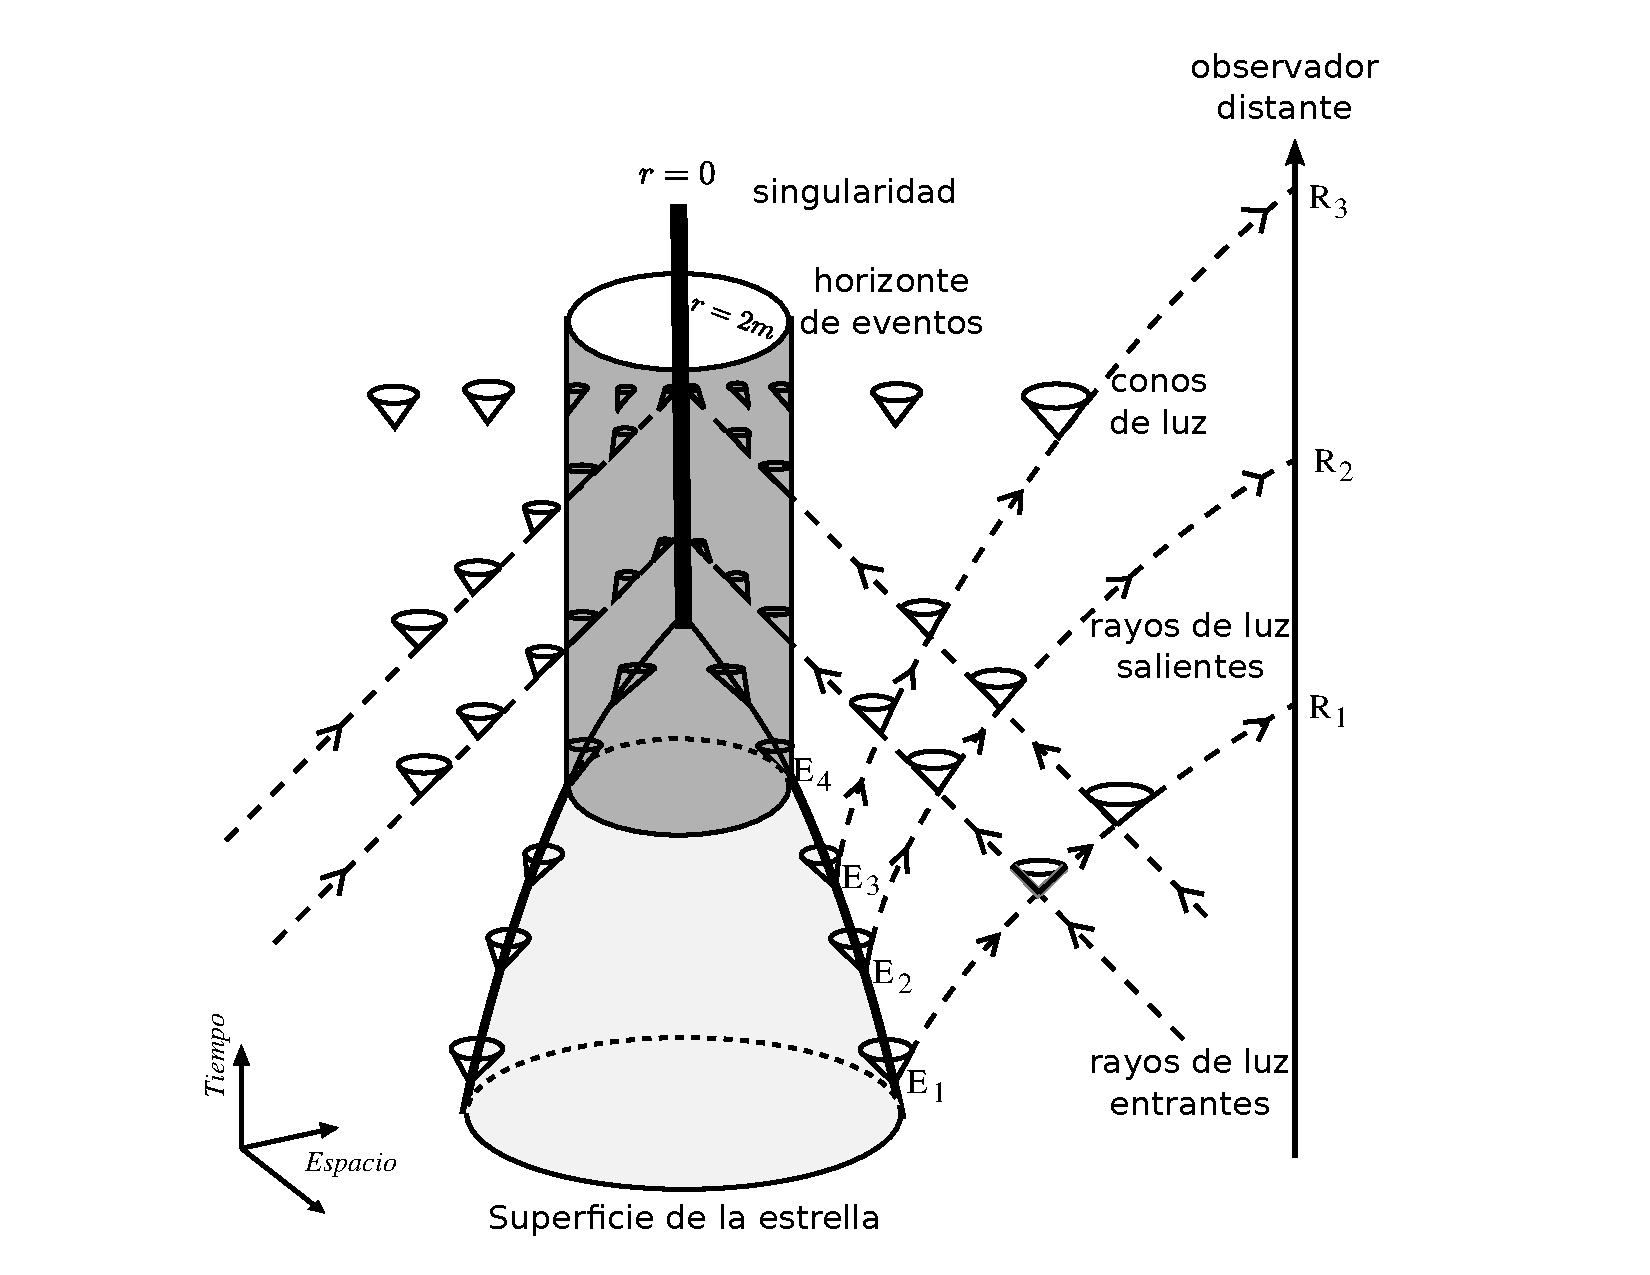
\includegraphics[height=6cm]{fig/fig-colapso.pdf}
\caption{Colapso estelar, figura adaptada a partir de Ref. \cite{Luminet98}}
\label{fig:colapso}
\end{center}
\end{figure}
\chapter{Agujeros Negros Rotantes ***PRELIMINAR***}\label{cap:Kerr}

Luego de que Karl Schwarzchild  encontrara en 1916 la primera soluci\'on de agujero negro esf\'ericamente sim\'etrica de las ecuaciones de Einstein, pas\'o poco menos de medio siglo sin que alguien pudiera encontrar la soluci\'on de agujero negro rotante.  Roy Kerr\footnote{Roy Patrick Kerr (16 de mayo de 1934) matem\'atico neozeland\'es. Ver \url{http://es.wikipedia.org/wiki/Roy_Kerr}.} fue el que encontr\'o esta soluci\'on en su famoso trabajo de 1963 \cite{Kerr63}, comenzando as\'i la llamada ``edad de oro'' de los agujero negros, periodo de alrededor de dos d\'ecadas donde hubo una considerable renovaci\'on en la f\'isica de estos objetos, que son el modelo usado para describir los agujeros negros astrof'isicos.

Existen tres cantidades que en teor\'ia describen completamente a un agujero negro: su masa, su momentum angular y su carga. La soluci\'on m\'as conocida es la que tiene momentum angular y carga nula: el agujero negro de Schwarzschild. Si el agujero negro tiene s\'olo carga nula es llamado de Kerr. Si tiene momentum angular nulo es llamado agujero negro de Reissner-Nordstrom y en el caso de que ninguna de las cantidades sea nula es llamado agujero negro de Kerr-Newman. 

%En el presente cap\'itulo se har\'a enf\'asis de la soluci\'on de Kerr, donde se estudiar\'an un buen n\'umero de propiedades asociadas a la soluci\'on, como la existencia de diversos horizontes de eventos, zonas dentro del agujero donde las part'iculas tienen la posibilidad de escapar o de usar al agujero negro como una fuente de energ\'ia, entre otras.


\section{Soluci\'on de Kerr}
La soluci\'on de Kerr en la \textit{forma de Boyer-Lindquist} es dada por el siguiente elemento de l\'inea:
 \begin{equation}
ds^2=\frac{\Delta}{\rho^2}(cdt-a\sen^2\theta d\varphi)^2-\frac{\sen^2\theta}{\rho^2}\left[(r^2+a^2)d\varphi-acdt \right]^2-\frac{\rho^2}{\Delta}dr^2-\rho^2d\theta^2, \label{BL}
 \end{equation}
donde
\begin{equation}
\rho^2:=r^2+a^2\cos^2\theta,\qquad \Delta=r^2-2mr+a^2.
\end{equation}
Al realizar la transformaci\'on de coordenadas definida por
\begin{equation}
\begin{aligned}
cd\bar{t}&=cdt+\frac{2mr}{\Delta}dr,\\
x&=r\sen\theta\cos\varphi+a\sen\theta\sen\varphi, \\
y&=r\sen\theta\sen\varphi-a\sen\theta\cos\varphi, \\
z&=r\cos\theta,   \label{zrt}
\end{aligned}
\end{equation}
se obtiene, a partir de \eqref{BL}, la soluci\'on de Kerr en la forma original en la que fue encontrada, es decir, en la \textit{forma de Kerr} \cite{Kerr63} (ver tambi'en \cite{Kerr65}),
\begin{align}
ds^2 &= c^2d\bar{t}^2-dx^2-dy^2-dz^2 \nonumber \\
&\quad -\frac{2mR^3}{R^4+a^2z^2}\left(cd\bar{t}+\frac{R}{R^2+a^2}(xdx+ydy)+\frac{a}{R^2+a^2}(ydx-xdy)+\frac{z}{R}dz \right)^2 , \label{Kerr}
\end{align}
donde $R(x,y,z)$ satisface
\begin{equation}
R^4 - (x^2+y^2+z^2-a^2)R^2 -a^2z^2=0.
\end{equation}

Algunas primeras caracter\'isticas destacables de esta soluci\'on es que es estacionaria y tiene simetr\'ia axial, ya que los coeficientes m\'etricos no depende de $t$ ni de $\varphi$ (por lo tanto $\partial_t$ y $\partial_\phi$ son vectores de Killing). Adem'as, la m\'etrica es invariante bajo reflexiones de estas coordenadas y, debido a la forma del elemento de l\'inea, es equivalente a decir que es invariante bajo las transformaciones
\begin{equation}
t\rightarrow -t, \qquad a\rightarrow -a.
\end{equation}

Para interpretar las constantes $m$ y $a$ podemos reordenan los t\'erminos de \eqref{BL} de la siguiente manera:
\begin{equation}
\begin{aligned}\label{BL2}
ds^2&=\left(1-\frac{2mr}{\rho^2}\right)c^2dt^2-\frac{\rho^2}{\Delta}dr^2-\rho^2d\theta^2-\left(r^2+a^2+\frac{2mra^2\sen^2 \theta}{\rho^2}\right)\sen^2\theta\,d\varphi^2\\
&\qquad+\frac{4amr\sen^2\theta}{\rho^2}d\varphi(cdt) .
\end{aligned}
\end{equation}
Utilizando coordenadas isotr\'opicas, dadas por la transformaci\'on de coordenadas
\begin{equation}
r=\bar{r}\left(1+\frac{m}{2\bar{r}}\right)^2,
\end{equation}
y considerando s\'olo t\'erminos de primer orden en $m/\bar{r}$ y $a/\bar{r}$, encontramos
\begin{equation}
ds^2 =\left(1-\frac{2m}{\bar{r}} \right)c^2dt^2-\left(1+\frac{2m}{\bar{r}} \right)\left[d\bar{r}^2+\bar{r}^2d\Omega^2\right]+\frac{4am}{\bar{r}}\sen^2\theta d\varphi(cdt)+\mathcal{O}(G^2) .\label{BL3}
\end{equation}

Al comparar \eqref{BL3} con \eqref{dssss2}, que describe la geometr\'ia del espacio-tiempo de una masa esf\'erica que rota con momentum angular constante $J$, vemos que esta soluci'on tiene momento angular no nulo, proporcional al par\'ametro $a$, que ser\'a llamado \textbf{par\'ametro de rotaci'on}. M'as espec'ificamente, obtenemos que el momento angular de la soluci'on es
\begin{equation}
J=aMc,
\end{equation}
$M=mc^2/G$ es la masa del agujero negro.
%
%Resumiendo, la m\'etrica de Kerr en coordenadas de Boyer-Lindquist viene dada por la expresi\'on
%\begin{equation}
%\boxed{ds^2=\frac{\Delta}{\rho^2}(cdt-a\sen^2\theta d\varphi)^2-\frac{\sen^2\theta}{\rho^2}\left[(r^2+a^2)d\varphi-acdt \right]^2-\frac{\rho^2}{\Delta}dr^2-\rho^2d\theta^2}, 
%\end{equation}
%donde,
%\begin{equation*}
%\begin{aligned}
%\rho^2&=r^2+a^2\cos^2 \theta ,\\
%\Delta&=r^2-2mr+a^2.
%\end{aligned}
%\end{equation*}

%\subsection{M\'etodo de Newman y Janis}
%
%Newman\footnote{Ezra Ted Newman (17 de octubre de 1929) f\'isico estadounidense \url{http://en.wikipedia.org/wiki/Ezra_T._Newman}.} y Janis encontraron un \'util m\'etodo para ``agregarle rotaci\'on'' a las soluciones, as\'i por ejemplo, se puede pasar desde la soluci\'on de Schwarzschild a la de Kerr o de la soluci\'on de Reissner-Nordstrom a la de Kerr-Newman.
%
%\subsubsection{La Tetrada Nula}
%
%Sea el conjunto de vectores contravariantes linealmente independientes $\left\lbrace e^{\, \mu}_a \right\rbrace_{a=1,4}$, donde $a$ etiqueta a cada vector definidos en un punto de una variedad. Este conjunto es llamado ``tetrada'' o ``frame'' (vierbein). Se define  entonces punto a punto la matriz de escalares $g_{ab}$, dada por
%\begin{equation}
%g_{ab}(x)=g_{\mu \nu}(x)e^{\,\mu}_a(x)e^{\,\nu}_b(x) \label{gij}
%\end{equation}
%
%Como los vectores son linealmente independientes, y suponiendo que $g_{\mu \nu}$ es no singular, entonces $g_{ab}$ es no singular. Con ello se demuestra la existencia de su inversa $g^{ab}$, satisfaci\'endose la siguiente identidad
%\begin{equation}
%g^{ab}g_{bc}=\delta^{a}_{\,c}.
%\end{equation}
%
%Una relaci\'on a utilizarse m\'as adelante es \eqref{gab}, que se puede obtener contrayendo \eqref{gij} con los vectores de la base (del espacio tangente) dual a $e^{\,\mu}_{a}$, dada por $e^{\,a}_{\mu}$ tal que $e^{\,\mu}_{a}e^{\,a}_{\nu}=\delta^{\mu}_{\nu}$ y $e^{\,\mu}_{a}e^{\,b}_{\mu}=\delta^{a}_{b}$.\\
%
%\begin{equation}
%g_{\mu \nu}(x)=g_{ab}(x) e^{\,a}_{\mu}(x)e^{\,b}_{\nu}(x).  \label{gab}
%\end{equation}
%
%Sea la tetrada $(v^{\mu},i^{\mu},j^{\mu},k^{\mu})$ donde $v^{\mu}$ es un vector tipo tiempo e $i^{\mu}, j^{\mu}$ y $k^{\mu}$ vectores tipo espacio, donde la m\'etrica del frame viene dada por la m\'etrica de Minkowski, es decir, $g_{ab}=\eta_{ab}=diag(1,-1,-1,-1)$.\\
%
%La idea es buscar un conjunto $(l^{\mu},n^{\mu},m^{\mu},p^{\mu})$ compuesto de vectores nulos (tipo luz) a partir de la tetrada en la que las relaciones ortonormalidad vienen dadas por la m\'etrica de Minkowski. Se definen entonces los dos primeros vectores del conjunto
%\begin{eqnarray} \label{l}
%l^{\mu}&:=\frac{1}{\sqrt{2}}(v^{\mu}+i^{\mu}),\\ \label{n}
%n^{\mu}&:=\frac{1}{\sqrt{2}}(v^{\mu}-i^{\mu}).
%\end{eqnarray}
%
%De \eqref{l} y \eqref{n} se puede verificar que los vectores construidos son efectivamente nulos 
%\begin{equation*}
%\begin{aligned}
%l^{\mu}l_{\mu}&=\frac{1}{2}(v^{\mu}+i^{\mu})(v_{\mu}+i_{\mu})\\
%&=\frac{1}{2}(v^{\mu}v_{\mu}+i^{\mu}i_{\mu})\\
%&=\frac{1}{2}(1-1)\\
%&=0,
%\end{aligned}
%\end{equation*}
%
%\begin{equation*}
%\begin{aligned}
%n^{\mu}n_{\mu}&=\frac{1}{2}(v^{\mu}-i^{\mu})(v_{\mu}-i_{\mu})\\
%&=\frac{1}{2}(v^{\mu}v_{\mu}+i^{\mu}i_{\mu})\\
%&=\frac{1}{2}(1-1)\\
%&=0.
%\end{aligned}
%\end{equation*}
%
%Y  adem\'as cumplen que $l^{\mu}n_{\mu}=1$, como se verifica a continuaci\'on :
%
%\begin{equation*}
%\begin{aligned}
%l^{\mu}n_{\mu}&=\frac{1}{2}(v^{\mu}+i^{\mu})(v_{\mu}-i_{\mu})\\
%&=\frac{1}{2}(v^{\mu}v_{\mu}-i^{\mu}i_{\mu})\\
%&=\frac{1}{2}(1+1)\\
%&=1.
%\end{aligned}
%\end{equation*}
%
%Por \'ultimo, es \'util que los vectores restantes que son combinaciones del conjunto de vetores $(j^{\mu},k^{\mu})$ sean complejos y de la forma
%\begin{eqnarray} \label{m}
%m^{\mu}&:=\frac{1}{\sqrt{2}}(j^{\mu}+ik^{\mu}),\\ \label{p}
%p^{\mu}&:=\frac{1}{\sqrt{2}}(j^{\mu}-ik^{\mu}).
%\end{eqnarray}
%
%Donde se oberva que $p^{\mu}=\bar{m}^{\mu}$.  Se puede verificar que los vectores encontrados tambi\'en son vectores nulos
%\begin{equation}
%m^{\mu}m_{\mu}=0,
%\end{equation}
%
%\begin{equation}
%\bar{m}^{\mu}\bar{m}_{\mu}=0.
%\end{equation}
%
%Otra relaci\'on importante que satisfacen estos vectores es que
%\begin{equation*}
%\begin{aligned}
%m^{\mu}\bar{m}_{\mu}&=\frac{1}{2}(j^{\mu}+ik^{\mu})(j_{\mu}-ik_{\mu})\\
%&=\frac{1}{2}(j^{\mu}j_{\mu}+k^{\mu}k_{\mu})\\
%&=\frac{1}{2}(-1-1)\\
%&=-1.
%\end{aligned}
%\end{equation*}
%
%Se puede escoger al conjunto de vectores encontrado como la tetrada nula
%\begin{equation}
%(e^{\,\mu}_0,e^{\,\mu}_1,e^{\,\mu}_2,e^{\,\mu}_3)=(l^{\mu},n^{\mu},m^{\mu},\bar{m}^{\mu}).
%\end{equation}
%
%Utilizando \eqref{gij} se demuestra que la m\'etrica de esta base viene dada por
%\begin{equation}
%g_{ab}=%
%\begin{pmatrix}
%0 & 1 & 0 & 0\\
%1 &0 & 0 & 0\\
%0 & 0 & 0 & -1\\
%0 & 0 & -1 & 0
%\end{pmatrix}.
%\end{equation}
%
%De \eqref{gab} se tiene que
%\begin{equation*}
%\begin{aligned}
%g_{\mu\nu}&=g_{ab}e^{\,a}_{\mu}e^{\,b}_{\nu} \\
%&=g_{01}e^{\,0}_{\mu}e^{\,1}_{\nu}+g_{10}e^{\,1}_{\mu}e^{\,0}_{\nu}+g_{23}e^{\,2}_{\mu}e^{\,3}_{\nu}+g_{32}e^{\,3}_{\mu}e^{\,2}_{\nu} \\
%&=l_{\mu}n_{\nu}+n_{\mu}l_{\nu}-m_{\mu}\bar{m}_{\nu}-\bar{m}_{\mu}m_{\nu}
%\end{aligned}
%\end{equation*}
%
%Por lo tanto, las componentes de $g_{\mu \nu}$ descompuesta en los vectores de la tetrada nula son
%\begin{equation}
%\boxed{g_{\mu \nu}=l_{\mu}n_{\nu}+n_{\mu}l_{\nu}-m_{\mu}\bar{m}_{\nu}-\bar{m}_{\mu}m_{\nu}}.
%\end{equation}
%
%De la relaci\'on \'anterior, se deduce que las componentes contravariantes vienen dadas por
%\begin{equation}\label{cv}
%\boxed{g^{\mu \nu}=l^{\mu}n^{\nu}+n^{\mu}l^{\nu}-m^{\mu}\bar{m}^{\nu}-\bar{m}^{\mu}m^{\nu}}.
%\end{equation}
%
%\subsubsection{Complexificaci\'on de la soluci\'on de Schwarzschild y soluci\'on de Kerr}
%
%Utilizando \eqref{Sch} y el cambio de variables de Eddington-Finkelstein dada por \eqref{tEF}, se tiene que
%\begin{equation}
%\begin{aligned}
%dt&=d\left(\bar{t}-\frac{2m}{c}\ln\left|r-2m\right| \right) \\
%&=d\bar{t}-\frac{2m}{c}\frac{dr/r}{\left(1-\frac{2m}{r} \right)}\\
%\end{aligned}
%\end{equation}
%
%con lo cual
%\begin{equation}
%dt^2=d\bar{t}^2-\frac{4m}{c}\frac{d\bar{t}dr/r}{\left(1-\frac{2m}{r} \right)}+\frac{4m^2}{c^2}\frac{dr^2/r^2}{\left(1-\frac{2m}{r} \right)^2} \label{t2ef}
%\end{equation}
%
%Reemplazando \eqref{t2ef} en \eqref{Sch}, se obtiene lo siguiente
%\begin{equation}
%ds^2=\left( 1-\frac{2m}{r}\right) (cd\bar{t})^2-\frac{4m}{c}cd\bar{t}dr-\left( 1+\frac
%{2m}{r}\right)dr^2-r^2d\Omega^2
%\end{equation}
%
%Introduciendo el par\'ametro de tiempo avanzado,
%\begin{equation}
%v:=c\bar{t}+r
%\end{equation}
%
%Reescribimos el elemento de l\'inea de Schwarzschild en coordenadas avanzadas de Eddington-Finkelstein tiene la siguiente forma
%\begin{equation}
%\boxed{ds^2=\left(1-\frac{2m}{r}\right)dv^2-2dvdr-r^2d\theta^2-r^2\sen^
%2\theta d\varphi^2} \label{ds2ef}
%\end{equation}
%
%Cabe destacar que el elemento de l\'inea \eqref{ds2ef} en estas coordenadas es una especie de extensi\'on anal\'itica de la soluci\'on de Schwarzshild dada en \eqref{Sch}. Expl\'icitamente, las componentes $g_{\mu \nu}$ en las coordenadas $x^{\mu}=(v,r,\theta,\varphi)$ son
%\begin{equation}
%g_{\mu \nu}=%
%\begin{pmatrix}
%1-\frac{2m}{r} & -1 & 0 & 0\\
%-1 &0 & 0 & 0\\
%0 & 0 & -r^2 & 0\\
%0 & 0 & 0& -r^2\sen^2 \theta
%\end{pmatrix}.
%\end{equation}
%
%As\'i, $g^{\mu \nu}$ viene dado por
%\begin{equation}
%g^{\mu \nu}=%
%\begin{pmatrix}
%0 & -1 & 0 & 0\\
%-1 &- \left(1-\frac{2m}{r}\right) & 0 & 0\\
%0 & 0 & -\frac{1}{r^2} & 0\\
%0 & 0 & 0 & -\frac{1}{r^2\sen^2\theta}
%\end{pmatrix}.
%\end{equation}
%
%Dentro de las infinitas soluciones que satisfacen \eqref{cv}, se puede verificar que una de ellas es la siguiente 
%\begin{equation}
%\begin{aligned}
%l^{\mu}&=(0,1,0,0),\\
%n^{\mu}&=\left(-1,-\frac{1}{2}\left(1-\frac{2m}{r}\right),0,0 \right),\\
%m^{\mu}&=\left(0,0,\frac{1}{r\sqrt{2}},\frac{i}{r\sqrt{2}\sen \theta} \right).\\
%\end{aligned}
%\end{equation}
%
%Ahora, el truco comienza haciendo que $r$ tenga valores complejos, luego
%\begin{equation}
%\frac{2}{r}\rightarrow \frac{1}{r}+\frac{1}{\bar{r}}.
%\end{equation}
%
%Entonces se puede re-escribir la tetrada de la siguiente forma
%\begin{equation}
%\begin{aligned}
%l^{\mu}&=(0,1,0,0),\\
%n^{\mu}&=\left(-1,-\frac{1}{2}\left(1-m\left(\frac{1}{r}+\frac{1}{\bar{r}} \right) \right),0,0 \right),\\
%m^{\mu}&=\left(0,0,\frac{1}{r\sqrt{2}},\frac{i}{r\sqrt{2}\sen \theta} \right).\\
%\end{aligned}
%\end{equation}
%
%Luego, se hace una transformaci'on compleja en la coordenadas $v$ y $r$ dejando las otras coordenadas invariantes, tal que las nuevas coordenadas $v'$ y $r'$ sean reales
%\begin{equation}
%\begin{aligned}
%v'&=v+ia\cos \theta, \\
%r'&=r+ia\cos \theta. \\
%\end{aligned}
%\end{equation}
%
%Un vector $V^{\mu}$, bajo una transformaci\'on general de coordenadas $x'^{\mu}=x'^{\mu}(x^{\nu})$, transforma como
%\begin{equation}
%V'^{\mu}(x')=\frac{\partial x'^{\mu}}{\partial x^{\nu}}(x')V^{\nu}(x').
%\end{equation}
%
%Luego, los vectores en las nuevas coordenadas quedan de la siguiente forma
%\begin{equation}
%\begin{aligned}
%l'^{\mu}&=(0,1,0,0),\\
%n^{\mu}&=\left(-1,-\frac{1}{2}\left(1-\frac{2mr'}{r'^2+a^2\cos^2\theta}\right),0,0 \right),\\
%m^{\mu}&=\frac{1}{\sqrt{2}(r'+ia\cos \theta)}\left(-ia\sen \theta,-ia\sen \theta,1,\frac{i}{\sen \theta} \right).\\
%\end{aligned}
%\end{equation}
%
%De \eqref{cv} se tiene que
%\begin{equation}\label{delta}
%g'^{\mu \nu}=%
%\begin{pmatrix}
%-\frac{a^2\sen^2\theta}{r'^2+a^2\cos^2\theta} & -1-\frac{a^2\sen^2\theta}{r'^2+a^2\cos^2\theta}  & 0 & \frac{a}{r'^2+a^2\cos^2\theta} \\
%-1 -\frac{a^2\sen^2\theta}{r'^2+a^2\cos^2\theta} &- 1+\frac{2mr'-a^2\sen^2\theta}{r'^2+a^2\cos^2\theta}  & 0 &\frac{a}{r'^2+a^2\cos^2\theta} \\
%0 & 0 & -\frac{1}{r'^2+a^2\cos^2\theta} & 0\\
%\frac{a}{r'^2+a^2\cos^2\theta} & \frac{a}{r'^2+a^2\cos^2\theta} & 0 & -\frac{1}{\sen^2\theta(r'^2+a^2\cos^2\theta)}
%\end{pmatrix}.
%\end{equation}
%
%Haciendo que $(v',r') \rightarrow (v,r)$, definiendo $\rho^2:=r^2+a^2\cos^2\theta$ y utilizando \eqref{delta}, la inversa de $g'^{\mu \nu}$ es
%\begin{equation}
%g'_{\mu \nu}=%
%\begin{pmatrix}
%1-\frac{2mr}{\rho^2} & -1 & 0 & -\frac{2mr}{\rho^2}a\sen^2\theta\\
%-1 &0 & 0 & -a\sen^2\theta\\
%0 & 0 & -\rho^2 & 0\\
%-\frac{2mr}{\rho^2}a\sen^2\theta & -a\sen^2\theta& 0 & -\left((r^2+a^2)\sen^2\theta+\frac{2mr}{\rho^2}a^2\sen^4\theta \right)
%\end{pmatrix}. \label{mkerr}
%\end{equation}
%
%Aqu\'i \eqref{mkerr} representa a la m\'etrica de la soluci\'on de Kerr en la \textit{forma de las coordenadas avanzadas de Eddington-Finkelstein}, donde el elemento de l\'inea viene dado por
%\begin{equation}
%ds^2=\left(1-\frac{2mr}{\rho^2} \right)dv^2+\frac{4mr}{\rho^2}a\sen^2\theta dvd\bar{\varphi}+2a\sen^2\theta drd\bar{\varphi}-\rho^2d\theta^2-\left((r^2+a^2)\sen^2\theta+\frac{2mr}{\rho^2}a^2\sen^4\theta \right)d\bar{\varphi}^2. \label{EF}
%\end{equation}
%
%Esta m\'etrica es una soluci\'on de las ecuaciones de Einstein en el vac\'io, ya que, como puede verificarse\footnote{Por ejemplo, usando el programa (wx)maxima, ver \url{http://maxima.sourceforge.net/es/}.}  anula el tensor de Einstein:
%\begin{equation}
%G_{\mu \nu}=0.
%\end{equation}
%
%Si se define
%\begin{equation}
%\Delta:=r^2-2mr+a^2,
%\end{equation}
%
%y se hacen las siguientes transformaciones de coordenadas
%\begin{equation}
%\begin{aligned}
%d\bar{\varphi}&=d\varphi+\frac{a}{\Delta}dr,\\
%dv&=cdt+\frac{2mr+\Delta}{\Delta}dr.
%\end{aligned}
%\end{equation}
% 
% Se obtiene la soluci\'on de Kerr en la \textit{forma de Boyer-Lindquist}, cuyo elemento de l\'inea es
% \begin{equation}
%ds^2=\frac{\Delta}{\rho^2}(cdt-a\sen^2\theta d\varphi)^2-\frac{\sen^2\theta}{\rho^2}\left[(r^2+a^2)d\varphi-acdt \right]^2-\frac{\rho^2}{\Delta}dr^2-\rho^2d\theta^2 . \label{BL}
% \end{equation}
%
%Por \'ultimo, al hacer la transformaci\'on de coordenadas
%\begin{equation}
%\begin{aligned}
%c\bar{t}&=v-r ,\\
%x&=r\sen\theta\cos\varphi+a\sen\theta\sen\varphi ,\\
%y&=r\sen\theta\sen\varphi-a\sen\theta\cos\varphi ,\\
%z&=r\cos\theta  .   \label{tck}
%\end{aligned}
%\end{equation}
%
%De \eqref{BL} se obtiene la soluci\'on de Kerr en la forma original en la que fue descubierta, es decir, en la \textit{forma de Kerr}
%\begin{equation}
%ds^2=c^2d\bar{t}^2-dx^2-dy^2-dz^2-\frac{2mr^3}{r^4+a^2z^2}\left(cd\bar{t}+\frac{r}{a^2+r^2}(xdx+ydy)+\frac{a}{a^2+r^2}(ydx-xdy)+\frac{z}{r}dz \right)^2 . \label{Kerr}
%\end{equation}
%
%Pero \eqref{Kerr} puede ser escrito en una forma mucho m\'as compacta
%\begin{equation}
%\boxed{ds^2=\eta_{\mu \nu}dx^{\mu}dx^{\nu}-\lambda l_{\mu}l_{\nu} dx^{\mu}dx^{\nu}.}
%\end{equation}
%
%Donde $\lambda=2mr^3/(r^4+a^2z^2)$ y $l_{\mu}$ es un vector nulo dado por
%\begin{equation}
%l_{\mu}=\left(1,\frac{rx+ay}{a^2+r^2},\frac{ry-ax}{a^2+r^2},\frac{z}{r}\right)
%\end{equation}
%
%Al hacer $a=0$ se tiene que
%\begin{equation*}
%\begin{aligned}
%\rho^2&=r^2 , \\
%\Delta&= r^2-2mr .
%\end{aligned}
%\end{equation*}
%
%Y reemplazando en \eqref{BL}, se obtiene m\'etrica de Schwarzschild exterior en coordenadas de curvatura. En efecto
%\begin{equation}
%\begin{aligned}
%ds^2&=\frac{r^2-2mr}{r^2}c^2dt^2-\frac{\sen^2\theta}{r^2}(r^2d\varphi)^2-\frac{r^2}{r^2-2mr}dr^2-r^2d\theta^2\\
%&=\left(1-\frac{2m}{r} \right)c^2dt^2-\frac{dr^2}{1-\frac{2m}{r}}-r^2(d\theta^2+\sen^2\theta d\varphi^2)\\
%&=\left(1-\frac{2m}{r} \right)c^2dt^2-\frac{dr^2}{1-\frac{2m}{r}}-r^2d\Omega^2 .
%\end{aligned}
%\end{equation}
%
%Si se define la coordenada esf\'erica radial como $R^2:=x^2+y^2+z^2=r^2+a^2\sen^2\theta$ y haciendo $R\rightarrow \infty$ con $r\gg a$, entonces elemento de l\'inea \eqref{BL} coincide con el de un espacio tiempo plano, esto es
%\begin{equation}
%ds^2=\eta_{\mu \nu}dx^{\mu}dx^{\nu} .
%\end{equation}
%
%En otras palabras la soluci\'on de Kerr es asint\'oticamente plana.\\
%
%Otras caracter\'isticas destacables de esta soluci\'on es que es estacionaria y tiene simetr\'ia axial ya que los coeficientes m\'etricos no depende de $t$ ni de $\varphi$ y que la m\'etrica es invariante bajo reflexiones de estas coordenadas y debido a la forma del elemento de l\'inea, es equivalente a decir que es invariante bajo las transformaciones
%\begin{equation}
%t\rightarrow -t, \qquad a\rightarrow -a.
%\end{equation}
%
%Otro punto a analizar es el rol que juega la constante $a$ en esta m\'etrica, para ello se reordenan los t\'erminos de \eqref{BL} de la siguiente manera
%\begin{equation}
%\begin{aligned}
%ds^2&=\left(1-\frac{2mr}{\rho^2}\right)c^2dt^2-\frac{\rho^2}{\Delta}dr^2-\rho^2d\theta^2-\left(r^2+a^2+\frac{2mra^2\sen^2 \theta}{\rho^2}\right)\sen^2\theta\,d\varphi^2\\
%&\qquad+\frac{4amr\sen^2\theta}{\rho^2}d\varphi(cdt) .\label{BL2}
%\end{aligned}
%\end{equation}
%
%Utilizando coordenadas isotr\'opicas, dadas por la transformaci\'on de coordenadas
%\begin{equation}
%r=\bar{r}^2\left(1+\frac{m}{2\bar{r}}\right)^2 .
%\end{equation}
%
%y considerando s\'olo t\'erminos de primer orden en $G$ con $\bar{r} \gg a$, entonces \eqref{BL2} tiene la siguiente forma
%\begin{equation}
%ds^2 =\left(1-\frac{2m}{\bar{r}} \right)c^2dt^2-\left(1+\frac{2m}{\bar{r}} \right)\left[d\bar{r}^2+\bar{r}^2d\Omega^2\right]+\frac{4am}{\bar{r}}\sen^2\theta d\varphi(cdt)+\mathcal{O}(G^2) .\label{BL3}
%\end{equation}
%
%Al comparar \eqref{BL3} con \eqref{dssss2} que describe la geometr\'ia del espacio-tiempo de una masa esf\'erica que rota con momentum angular constante $J$, devela la naturaleza de la soluci\'on de Kerr, que describe entonces un agujero negro rotante, con momento angular proporcional al par\'ametro $a$, que ser\'a llamado par\'ametro de giro. Al hacer el l\'imite de campo d\'ebil, en efecto, se despeja esta cantidad cuyo valor es
%\begin{equation}
%a=\frac{J}{Mc},
%\end{equation}
%donde $J$ es el momentum angular de la fuente de campo gravitacional y $M$ la masa del agujero negro.\\
%
%Resumiendo, la m\'etrica de Kerr en coordenadas de Boyer-Lindquist viene dada por la expresi\'on
%\begin{equation}
%\boxed{ds^2=\frac{\Delta}{\rho^2}(cdt-a\sen^2\theta d\varphi)^2-\frac{\sen^2\theta}{\rho^2}\left[(r^2+a^2)d\varphi-acdt \right]^2-\frac{\rho^2}{\Delta}dr^2-\rho^2d\theta^2}, 
%\end{equation}
%donde,
%\begin{equation*}
%\begin{aligned}
%\rho^2&=r^2+a^2\cos^2 \theta ,\\
%\Delta&=r^2-2mr+a^2.
%\end{aligned}
%\end{equation*}


\subsection{Singularidades y Horizontes de la Soluci\'on de Kerr}

El invariante de Riemann asociado a la m\'etrica de Kerr es
\begin{equation}
R^{\mu \nu \lambda \rho}R_{\mu \nu \lambda \rho}=\frac{48m^2\left(r^2-a^2\cos^2\theta \right)\left[\rho^4-16r^2a^2\cos^2\theta \right]}{\rho^{12}} .
\end{equation}

Se observa que existe s\'olo una singularidad instr\'inseca,  cuando $\rho=0$. Esto implica que $r^2+a^2\cos^2\theta=0$, entonces
$$r=0, \qquad \cos \theta=0.$$

Note que, utilizando \eqref{zrt}, se encuentra que la singularidad es un anillo  de radio $a$ en el plano $xy$, es decir,
\begin{equation}
x^2+y^2=a^2,\qquad z=0
\end{equation}

Este tipo de agujero negro, tiene asociada una \textit{superficie de redshift infinito}, es decir, una superficie desde la cual las se\~nales emitidas hacia puntos lejanos est'an infinitamente dilatadas temporalmente. Los radios de esta superficie se pueden encontrar utilizando el hecho que sobre ella $g_{00}=0$, entonces de \eqref{BL2} se tiene que
\begin{equation} \label{rsk}
g_{00}=0\quad\Rightarrow\quad r^2-2mr+a^2\cos^2 \theta=0 \quad \Rightarrow \quad \boxed{r_{s_{\pm}}(\theta)=m\pm\sqrt{m^2-a^2\cos^2\theta}.}
\end{equation}
As\'i, existen dos superficies $S_{+}$ y $S_{-}$, definidas por sus respectivos radios $r_{S_+}(\theta)$ y $r_{S_{-}}(\theta)$. Como los radios $r_{s_{\pm}}$ s'olo dependen de la coordenada $\theta$, estas superficies son axialmente sim\'etricas (superficies de revoluci'on en torno del eje $z$).

En el caso en que el par\'ametro de rotaci'on sea menor que el par\'ametro de masa del agujero negro $(a^2<m^2)$, la superficie $S_{+}$ posee un radio de $2m$ en el ecuador (plano $z=0$) y radio $m+\sqrt{m^2-a^2}$ en los polos, en tanto que la superficie $S_{-}$ est\'a contenida dentro de $S_{+}$. Ver figura \ref{fig:surface1}.
\begin{figure}[H]
 \centering
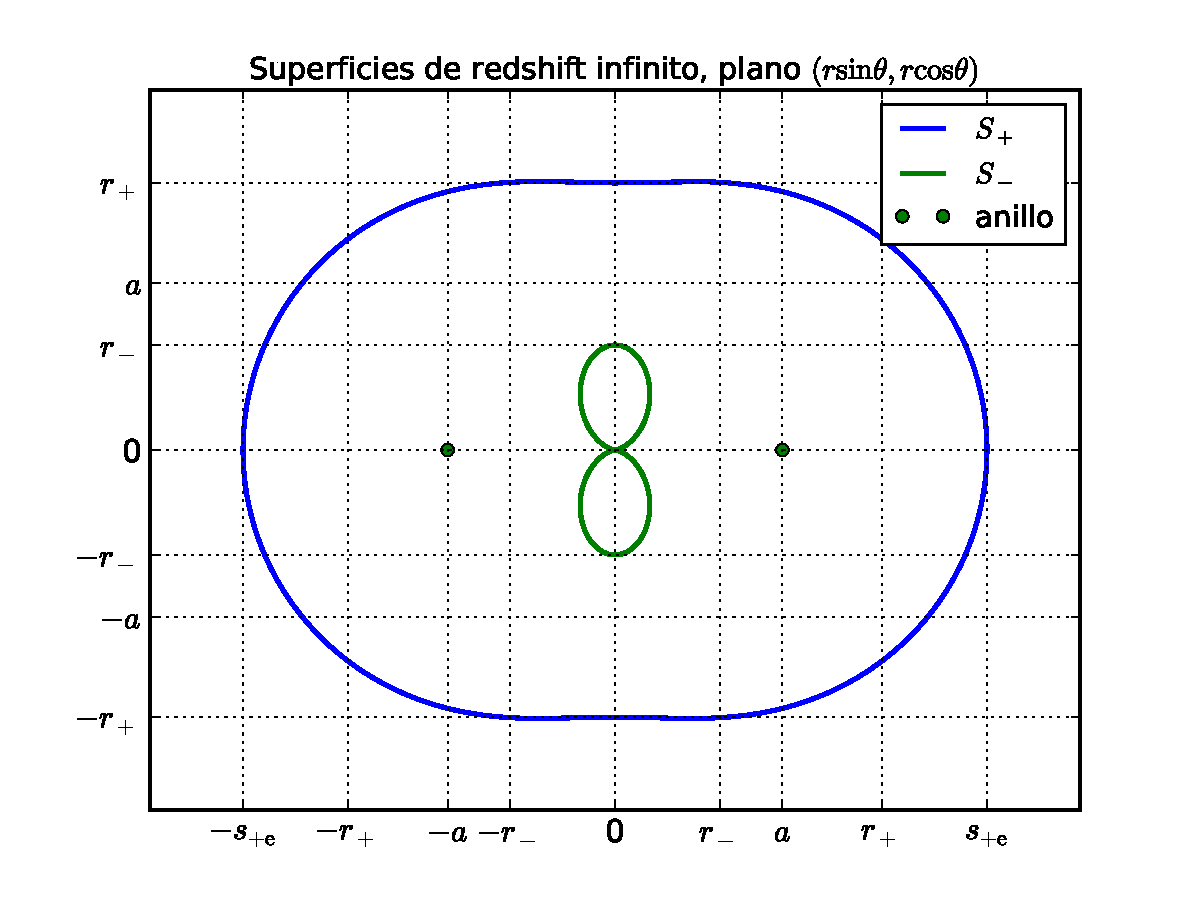
\includegraphics[height=7cm,angle=0]{fig/fig-superficies-1.pdf}
\caption{Superficies de redshift infinito. C'odigo Python \href{https://github.com/gfrubi/GR/blob/master/figuras-editables/fig-superficies-Kerr-01.py}{aqu\'i}.}
\label{fig:surface1}
\end{figure}
De \eqref{rsk} se observa que al hacer $a=0$, se obtiene lo ya sabido para la soluci\'on no rotante, donde $r_{S_{+}}$ coincide con el radio de
Schwarzschild $2m$ y el valor de $r_{S_{-}}$ con el de la singularidad.

Ahora, se buscar\'an superficies donde existan \textit{horizontes de eventos}. De \eqref{BL2} vemos que el horizonte estar'a ubicado en los puntos en los que $g_{rr}$ diverge, es decir, donde $\Delta$ se anula
\begin{equation}\label{grr}
g_{rr}=-\frac{\rho^2}{\Delta}\rightarrow -\infty \quad\Rightarrow\quad r^2-2mr+a^2=0.
\end{equation}
As\'i, los horizontes de eventos vienen dados por
\begin{equation}\label{horizontes}
\boxed{r_{\pm}=m\pm\sqrt{m^2-a^2}.}
\end{equation}
Note que estos horizontes existes s'olo si $a^2\leqslant m^2$. En el caso que $a^2>m^2$ se tiene que el campo gravitacional tiene una singularidad ``desnuda'' (debido a la no existencia de horizontes de eventos). La hip'otesis que esto no ocurre en la naturaleza es lo que se conoce como la \textit{Conjetura de Censura C\'osmica de Penrose}\footnote{Sir Roger Penrose (1931-) f\'isico-matem\'atico ingl\'es, \url{http://es.wikipedia.org/wiki/Roger_Penrose}.} que afirma que un colapso gravitacional que tiene condiciones iniciales bien comportadas nunca dar\'a origen a una singularidad desnuda. El agujero negro que tiene $a=m$ es llamado \textit{agujero negro maximalmente rotante}.\\

Luego, existen tres zonas (sin incluir la singualridad intr\'inseca) en las cuales la soluci\'on de Kerr es regular
\begin{equation}
\begin{aligned}
I&:\quad r_+<r<\infty\\
II&:\quad r_{-}<r<r_{+}\\
III&:\quad 0<r<r_{-}
\end{aligned}
\end{equation}

\begin{figure}[H]
 \centering
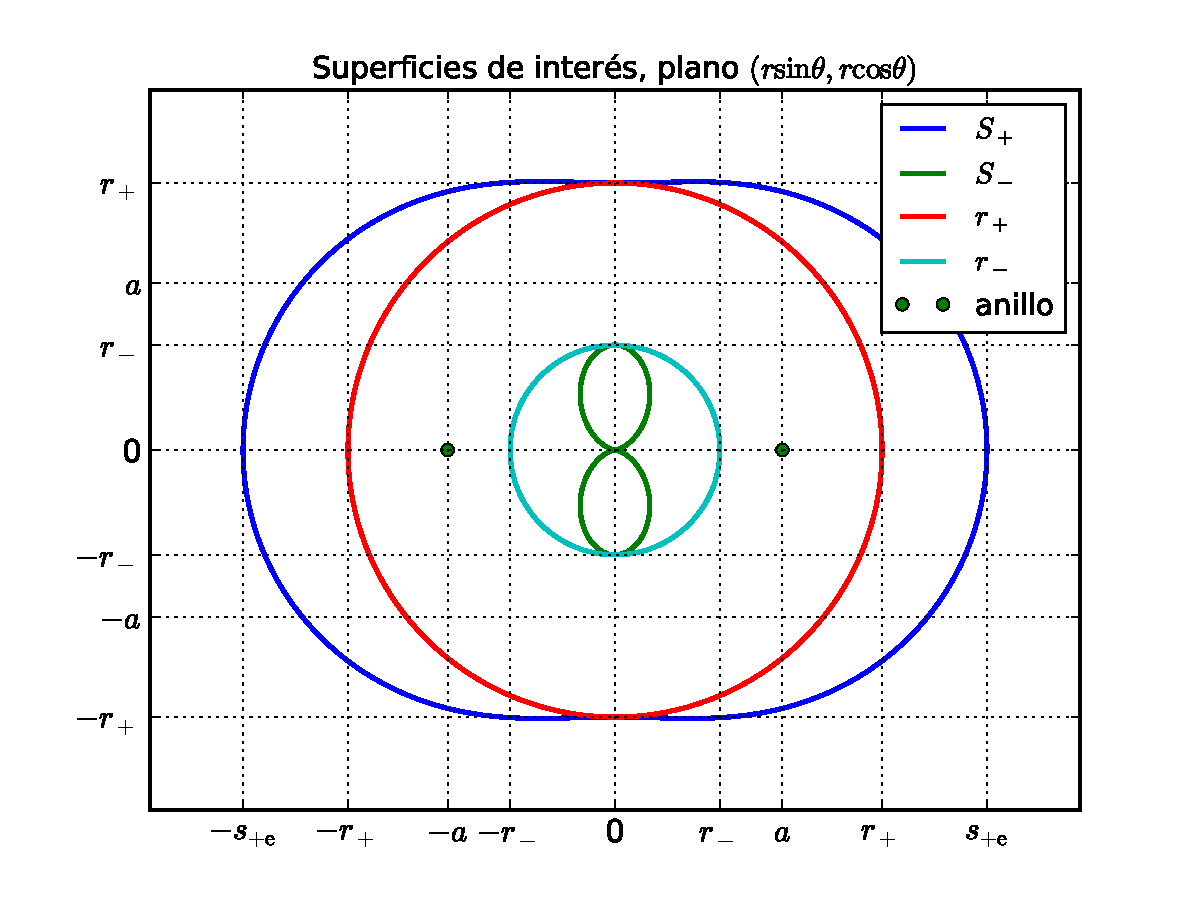
\includegraphics[height=7cm,angle=0]{fig/fig-superficies-2.pdf}
\caption{Horizontes y superficies de redshift infinito de la soluci\'on de Kerr.  C'odigo Python \href{https://github.com/gfrubi/GR/blob/master/figuras-editables/fig-superficies-Kerr-01.py}{aqu\'i}.}
\label{fig:surface2}
\end{figure}

Si $a=0$, entonces $r_{+}=2m$ y $r_{-}=0$, que tambi\'en coinciden con el radio de Schwarzschild y la singularidad intr\'inseca de ese caso. Se tiene que, como se mencion\'o anteriormente, en el caso de la soluci\'on de Schwarzschild $S_{+}$ coincide con el horizonte de eventos y $S_{-}$ con la singularidad en el origen.\\

Se define la \textit{Erg\'osfera} (del griego \textit{ergon} que significa trabajo) como la zona que existe entre la superficie de redshift infinito $S_{+}$ y el horizonte de eventos $r_{+}$(ver figura \ref{fig:surface2}), cuyas propiedades ser\'an analizadas m\'as adelante.\\

\begin{figure}[H]
 \centering
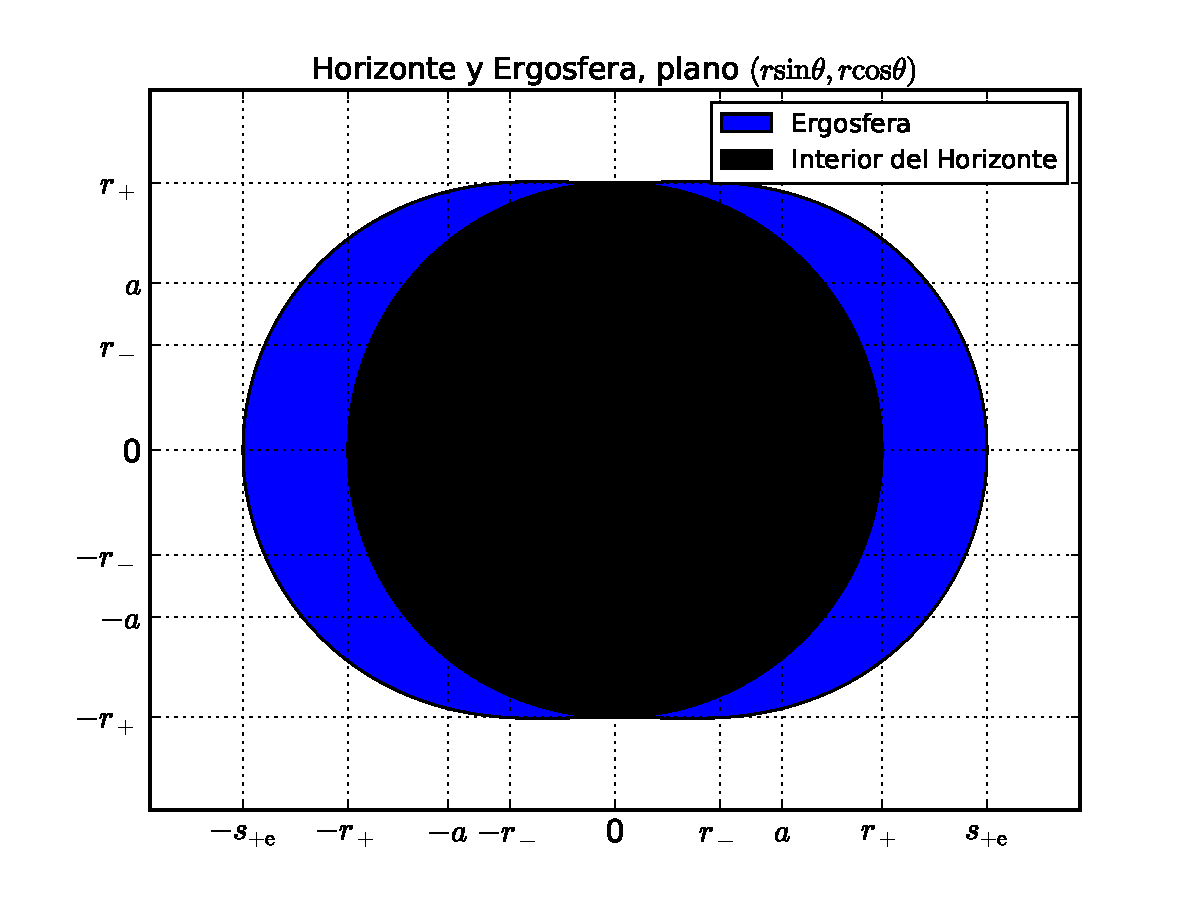
\includegraphics[height=7cm,angle=0]{fig/fig-superficies-3.pdf}
\caption{Horizonte de eventos y erg\'osfera de la soluci\'on de Kerr. C'odigo Python  \href{https://github.com/gfrubi/GR/blob/master/figuras-editables/fig-superficies-Kerr-01.py}{aqu\'i}.}
\label{fig:surface3}
\end{figure}

\subsection{Geod\'esicas tipo luz}

A diferencia de la soluci\'on de Schwarzschild en este caso no existen geod\'esicas nulas radiales, ya que no hay simetr\'ia esf\'erica. Sin embargo, s\'i es posible encontrar soluciones anal'iticas para el caso particular en que las trayectorias est'an contenidas en el cono definido por $\theta=\rm cte$. As\'i,
\begin{equation}
\theta={\rm cte},\qquad ds^2=0.
\end{equation}

Lo siguiente es resolver la ecuaci'on de la geod'esica para este caso. Sabemos que la ecuaci'on de la geod'esica puede ser derivada como las ecuaciones de Euler-Lagrange del lagrangiano efectivo dado, ver \eqref{gm1} y \eqref{gm4}, por
\begin{equation} \label{lagrange1}
\tilde{L}=\sqrt{-g_{\mu \nu}\dot{x}^{\mu}\dot{x}^{\nu}},
\end{equation}
donde la $\dot{x}^{\mu}=dx^\mu/d\lambda$ y $\lambda$ es alg'un par'ametro. Si bien podemos simplemente plantear la ecuaci'on de la geod'esica y resolverla, en esta secci'on haremos uso del siguiente hecho, que suministra un m'etodo alternativo (aunque equivalente), y que en algunos casos simplifica el c'alculo: Si $\lambda$ es un par\'ametro af\'in entonces la (misma) ecuaci'on geod'esica puede ser obtenida del siguiente lagrangeano ``alternativo'':
\begin{equation} \label{lagrange2}
\bar{L}= \frac{1}{2}g_{\mu \nu}\dot{x}^{\mu}\dot{x}^{\nu}.
\end{equation}
 
En el caso de la soluci'on de Kerr, este lagrangiano adopta la forma
\begin{equation}\label{lagrangeano1}
2\bar{L}=\frac{\Delta}{\rho^2}(c\dot{t}-a\sen^2\theta \dot{\varphi})^2-\frac{\sen^2\theta}{\rho^2}\left[(r^2+a^2)\dot{\varphi}-ac\dot{t} \right]^2-\frac{\rho^2}{\Delta}\dot{r}^2.
\end{equation}
Las ecuaciones de Euler-Lagrange vienen entonces dadas por
\begin{equation}\label{el}
\frac{\partial \bar{L}}{\partial x^{\mu}}-\frac{d}{d\lambda}\left(\frac{\partial \bar{L}}{\partial \dot{x}^{\mu}} \right)=0.
\end{equation}

Utilizando $x^0=ct$ en \eqref{el}, se obtiene la primera ecuaci\'on de movimiento:
\begin{equation}\label{elt}
\frac{\partial\bar{L}}{\partial c\dot{t}}=:l.
\end{equation}
 
Donde $l$ es una constante de integraci\'on. Desarrollando \eqref{elt}, se tiene lo siguiente:
\begin{equation}\label{11}
\frac{\Delta}{\rho^2}\left(c\dot{t}-a\sen^2 \theta \dot{\varphi}\right)+\frac{a\sen^2 \theta}{\rho^2}\left[(r^2+a^2)\dot{\varphi}-ac\dot{t} \right]=l.
\end{equation} 
 
 Ahora se buscar\'a la ecuaci\'on de movimiento correspondiente a $x^3=\varphi$, nuevamente de \eqref{el} se obtiene la siguiente ecuaci\'on de movimiento
 \begin{equation}\label{elp}
 \frac{\partial\bar{L}}{\partial \dot{\varphi}}=: -n,
 \end{equation}
 
donde $n$ tambi\'en es una constante de movimiento.\\

De \eqref{elp} se tiene que
\begin{equation}\label{22}
\frac{a\Delta \sen^2 \theta}{\rho^2}\left(c\dot{t}-a\sen^2 \theta \dot{\varphi}\right)+\frac{(r^2+a^2)\sen^2 \theta}{\rho^2}\left[(r^2+a^2)\dot{\varphi}-ac\dot{t} \right]=n.
\end{equation}
 
Usando el hecho que $ds^2=0$ y la expresi\'on \eqref{BL}, se tiene lo siguiente:
\begin{equation}\label{33}
\frac{\Delta}{\rho^2}(c\dot{t}-a\sen^2\theta \dot{\varphi})^2-\frac{\sen^2\theta}{\rho^2}\left[(r^2+a^2)\dot{\varphi}-ac\dot{t} \right]^2-\frac{\rho^2}{\Delta}\dot{r}^2=0.
\end{equation} 
 
Por \'ultimo utilizando $x^2=\theta$ y de \eqref{el}, se tiene que la ecuaci\'on de movimiento asociada a esta coordenada es
\begin{equation}
\frac{\partial }{\partial \theta}\left(g_{\mu \nu}\dot{x}^{\mu}\dot{x}^{\nu} \right)=0.
\end{equation} 

Desarrollando esta \'ultima expresi\'on se obtiene que
\begin{equation}\label{44}
\frac{a^2\Delta}{\rho^4}\left(c\dot{t}-a\sen^2 \theta \dot{\varphi} \right)^2-\frac{2a\Delta \dot{\varphi}}{\rho^2}\left(c\dot{t}-a\sen^2 \theta \dot{\varphi} \right)-\frac{(r^2+a^2)}{\rho^4}\left[(r^2+a^2)\dot{\varphi}-ac\dot{t} \right]^2+\frac{a^2\dot{r}^2}{\Delta}=0.
\end{equation}
 
Se obseva que s\'olo existen 3 inc\'ognitas ($\dot{t}$, $\dot{r}$ y $\dot{\varphi}$) y 4 ecuaciones, a saber, \eqref{11}, \eqref{22}, \eqref{33} y \eqref{44}. Por lo tanto, debe existir una expresi\'on que relacione los t\'erminos constantes $l$ y $n$. De \eqref{11} y \eqref{22} se obtienen las siguientes relaciones:
\begin{equation}\label{55}
\sen^2\theta \left[(r^2+a^2)\dot{\varphi}-ac\dot{t} \right]=(n-al\sen^2\theta),
\end{equation}
 
\begin{equation}\label{66}
\Delta(c\dot{t}-a\sen^2\theta\dot{\varphi})=\left[(r^2+a^2)l-an\right].
\end{equation}
 
De estas \'ultimas se puede despejar $\dot{\varphi}$, que viene dado por
\begin{equation}\label{77}
\dot{\varphi}=\frac{1}{\rho^2\sen^2\theta}(n-al\sen^2\theta)+\frac{a}{\rho^2\Delta}\left[(r^2+a^2)l-an\right].
\end{equation}
 
 Por otro lado, de \eqref{33} y \eqref{44} se tiene que
\begin{equation}\label{88}
 \frac{2a^2\Delta}{\rho^2}(c\dot{t}-a\sen^2\theta\dot{\varphi})^2 
 -2a\Delta \dot{\varphi}(c\dot{t}-a\sen^2\theta\dot{\varphi})-\frac{(r^2+a^2+a^2\sen^2\theta)}{\rho^2}\left[(r^2+a^2)\dot{\varphi}-ac\dot{t}\right]^2=0.
\end{equation}
 
 Reemplazando \eqref{55}, \eqref{66} y \eqref{77} en \eqref{88} se obtiene la ecuaci\'on que relaciona a $l$ y $n$:
 \begin{equation}
 (n+al\sen^2 \theta)(n-al\sen^2 \theta)=0.
 \end{equation}
 
Se escoger\'a la condici\'on $n-al\sen^2\theta=0$, que si es utilizada en \eqref{55} se tiene que
\begin{equation}\label{dott}
c\dot{t}=\frac{(r^2+a^2)}{a}\dot{\varphi}.
\end{equation}

Reemplazando \eqref{dott} en \eqref{11}, se puede despejar una expresi\'on para $\dot{\varphi}$
\begin{equation}\label{dotvar}
\dot{\varphi}=\frac{al}{\Delta}.
\end{equation}

As\'i, la ecuaci\'on para $c\dot{t}$ es
\begin{equation}\label{dott2}
c\dot{t}=\frac{(r^2+a^2)l}{\Delta}.
\end{equation}

Utilizando \eqref{dott} y \eqref{dotvar} en \eqref{33} se obtiene que
\begin{equation}
\dot{r}=\pm l.
\end{equation}

Luego, $r=\pm l\lambda+c$, donde $c$ es una constante, lo que entrega la libertad de elegir a $r$ como el par\'ametro af\'in a lo largo de cada geod\'esica, escogiendo en part\'icular $\dot{r}=+l$, se tiene de \eqref{dotvar} que
\begin{equation}\label{var1}
\frac{d \varphi}{dr}=\frac{\dot{\varphi}}{\dot{r}}=\frac{a}{\Delta}.
\end{equation}

Por otra parte de \eqref{dott2} se tiene que
\begin{equation}\label{t}
\frac{d(ct)}{dr}=\frac{c\dot{t}}{\dot{r}}=\frac{r^2+a^2}{\Delta}.
\end{equation}
 
Estas ecuaciones pueden ser integradas f\'acilmente. De \eqref{var1}  se tiene lo siguiente 
\begin{equation}
\begin{aligned}
\varphi(r)&=\int_{r_0}^r \frac{adr'}{\Delta} + \varphi_0\\
&=a\int_{r_0}^r\frac{dr'}{(r'-r_+)(r'-r_-)} + \varphi_0\\
&=\frac{a}{r_+-r_-}\int_{0}^r\left(\frac{1}{r'-r_+} - \frac{1}{r'-r_-} \right)dr'+\varphi_0\\
&=\frac{a}{r_+-r_-}\ln \left|\left(\frac{r-r_+}{r-r_-}\right)\left(\frac{r_0-r_-}{r_0-r_+} \right)\right| + \varphi_0.
\end{aligned}
\end{equation}
 
 Utilizando \eqref{horizontes} se tiene que 
 $$r_+-r_-=2\sqrt{m^2-a^2}.$$ 
 
 Considerando que $a^2<m^2$, se ecuentra que la expresi\'on para $\varphi$ como funci\'on de la coordenada $r$ de una curva que pasa por las coordenadas $(r_0,\varphi_0)$ es
\begin{equation}\label{congphi}
\boxed{\varphi(r)=\frac{a}{2\sqrt{m^2-a^2}}\ln \left|\left(\frac{r-r_+}{r-r_-}\right)\left(\frac{r_0-r_-}{r_0-r_+} \right)\right| + \varphi_0.}
\end{equation}  

De \eqref{t} se tiene que
\begin{equation}
\begin{aligned}
ct&=\int_{r_0}^r\frac{r'^2+a^2}{\Delta}dr'+ct_0\\
&=\int_{r_0}^r \frac{r'^2dr'}{(r'-r_+)(r'-r_-)}+a^2\int_{r_0}^r\frac{dr'}{(r'-r_+)(r'-r_-)}+ct_0.\\
\end{aligned}
\end{equation}

Se tiene adem\'as que
\begin{equation}
\int \frac{r^2dr}{(r-r_+)(r-r_-)}=r+\frac{r_{+}^2 \ln |r-r_+|}{r_+-r_-}-\frac{r_{-}^2\ln |r-r_-|}{r_+-r_-}.
\end{equation}

Luego
\begin{equation}
ct=r-r_0+\frac{(r_+^2+a^2)}{r_+-r_-}\ln\left|\frac{r-r_+}{r_0-r_+}\right|-\frac{(r_-^2+a^2)}{r_+-r_-}\ln \left|\frac{r-r_-}{r_0-r_-}\right|+ct_0.
\end{equation}

Al igual que en el c\'alculo de la expresi\'on para $\varphi$ se utiliza \eqref{horizontes} para encontrar lo siguiente
\begin{equation*}
r_{\pm}^2=m^2+\pm 2m\sqrt{m^2-a^2}+m^2-a^2.
\end{equation*}

As\'i, la expresi\'on buscada para $t$ como funci\'on de la coordenada $r$ de una curva que pasa por la coordenadas $(ct_0,r_0)$ es
\begin{equation}\label{congt}
\boxed{ct(r)=r-r_0+\left(m+\frac{m^2}{\sqrt{m^2-a^2}} \right)\ln\left|\frac{r-r_+}{r_0-r_+}\right|+\left(m-\frac{m^2}{\sqrt{m^2-a^2}} \right)\ln \left|\frac{r-r_-}{r_0-r_-}\right|+ct_0 .}
\end{equation}

Tal como se oberva en la figura \ref{fig:delta}, se tiene que $\Delta$ es positivo en las regiones $I$ y $III$, mientras que es negativo en la regi\'on $II$.

\begin{figure}[H]
 \centering
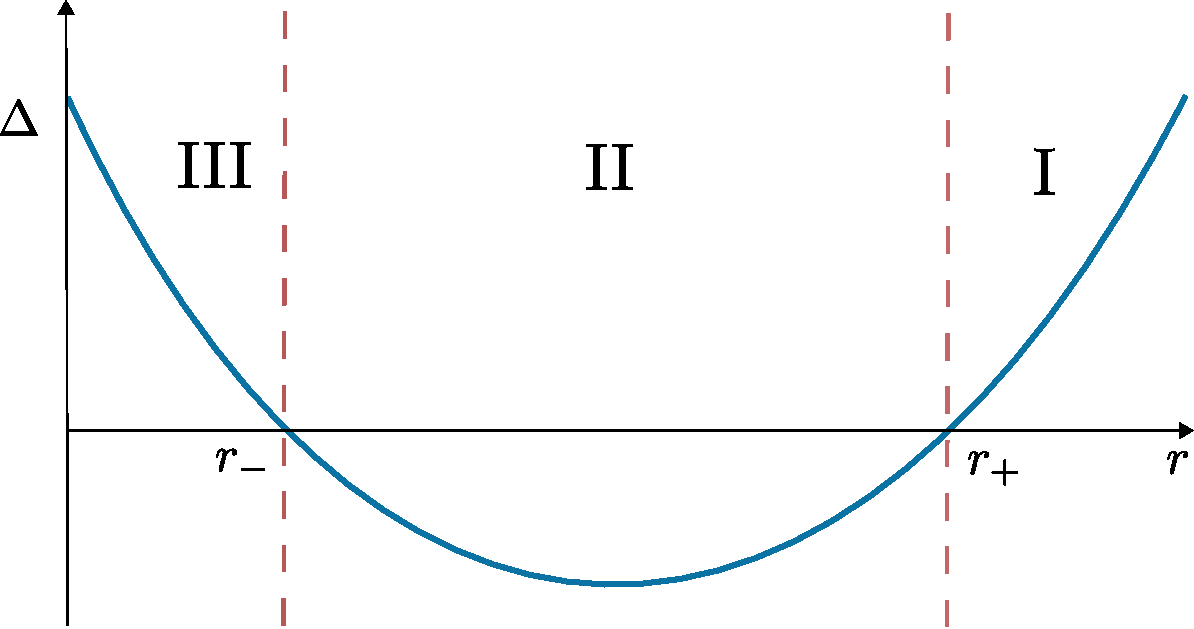
\includegraphics[height=4cm,angle=0]{fig/fig-delta.pdf}
\caption{Funci\'on $\Delta$ versus coordenada $r$}
\label{fig:delta}
\end{figure}

Como $\Delta >0$ en $I$ entonces $dr/dt>0$, as\'i las curvas son salientes en esta regi\'on con esta elecci\'on de signo en $\dot{r}$ ($\dot{r}=+l$),  a este conjunto de curvas (congruencia) se le llama \textit{congruencia principal de las geod\'esicas salientes tipo luz}. Mientras que si la elecci\'on es con signo negativo en $\dot{r}$, entonces $dr/dt<0$, donde esta congruencia es llamada \textit{congruencia principal de las geod\'esicas entrantes tipo luz}, cabe destacar que este caso es equivalente a hacer el cambio de signo simult\'aneamente en $ct$ y $\varphi$
\begin{equation}
\frac{dr}{dt}<0 \quad \Longleftrightarrow \quad ct \rightarrow -ct \quad \wedge \quad \varphi \rightarrow -\varphi .
\end{equation}

Por lo tanto, la expresi\'on para estas curvas es
\begin{equation}
\begin{aligned}
\varphi(r)&=-\frac{a}{2\sqrt{m^2-a^2}}\ln \left|\left(\frac{r-r_+}{r-r_-}\right)\left(\frac{r_0-r_-}{r_0-r_+} \right)\right| + \varphi_0 ,\\
ct(r)&=r_0-r-\left(m+\frac{m^2}{\sqrt{m^2-a^2}} \right)\ln\left|\frac{r-r_+}{r_0-r_+}\right|-\left(m-\frac{m^2}{\sqrt{m^2-a^2}} \right)\ln \left|\frac{r-r_-}{r_0-r_-}\right|+ct_0.\\
\end{aligned}
\end{equation}

Al hacer $a=0$ en \eqref{congphi} y \eqref{congt} se obtiene lo siguiente
\begin{equation}
\begin{aligned}
\varphi &=\varphi_0 ,\\
ct&=r-r_0+2m\ln|r-2m|+ct_0,\\
\end{aligned}
\end{equation}
que corresponden a las congruencias salientes, de la soluci\'on de Schwarzschild dadas en \eqref{rtfs} para el caso de part\'iculas tipo luz moviendose radialmente.\\

\subsection{Diagrama Espacio-Temporal}

Al representar gr\'aficamente la expresi\'on \eqref{congt} se obtiene el llamado diagrama espacio-temporal de los conos de luz (figura \ref{fig:conos1}), donde se observa que a medida que los conos se aproximan al horizonte de eventos $r_+$ en la regi\'on $I$ \'estos se empiezan a estrechar, hasta que la coordenada $t$ diverge, como es de esperar, ya que $r=r_+$ es una singularidad de las coordenadas. \'Esta puede ser removida al igual que en el caso de la soluci\'on de Schwarschild con un buen cambio de coordenadas.

 \begin{figure}[H]
 \centering
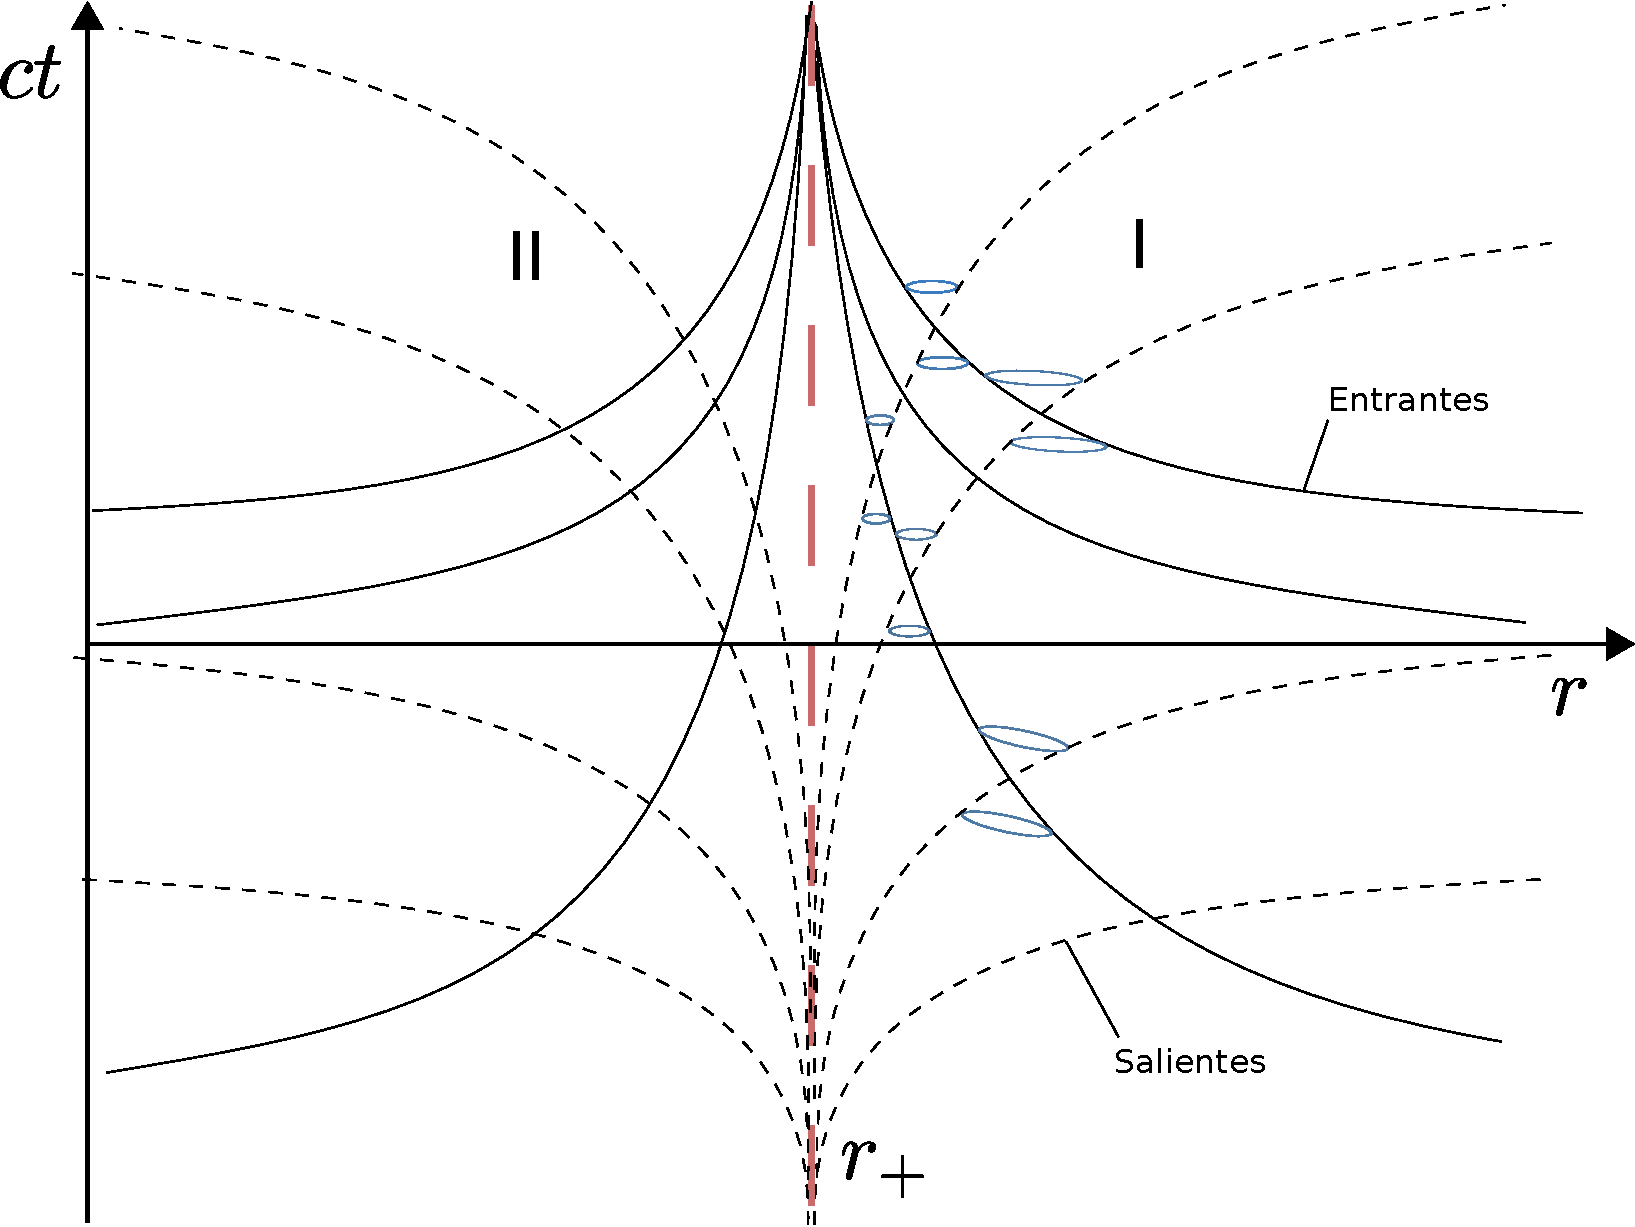
\includegraphics[height=6cm,angle=0]{fig/fig-conos1.pdf}
\caption{Diagrama espacio-tiempo en la vecindad de $r_+$}
\label{fig:conos1}
\end{figure}
  
Con ese prop\'osito se buscar\'a un an\'alogo al sistema de coordenadas de Eddington-Finkelstein utilizado en la soluci\'on de Schwarzschild. 

\subsubsection{Coordenadas de Eddington-Finkelstein} 

En el caso de la m\'etrica de Schwarzschild para extender las congruencias entrantes a trav\'es del horizonte de eventos $r=r_+$ se hac\'ia que las geod\'esicas tuvieran pendiente $-1$ en un diagrama espacio-tiempo durante todo su recorrido hasta llegar a la singularidad geom\'etrica, es decir, para encontrar las coordenadas de Eddington-Finkelstein $(c\bar{t},r,\varphi,\theta)$ se utiliz\'o la siguiente condici\'on: 
\begin{equation}
\frac{d(ct)}{dr}=-1 \quad \Rightarrow \quad d(ct)=-dr,
\end{equation}

Donde las coordenadas $(\varphi,\theta )$ eran constantes, esto es
\begin{equation}
d\varphi=0, \qquad d\theta=0 .
\end{equation}

En este caso se utilizar\'an las mismas condiciones, pero sobre las relaciones ya conocidas \eqref{t} y \eqref{var1}, utilizando $\dot{r}=-l$, as\'i
\begin{equation}
\begin{aligned}
d(ct)&=-\frac{r^2+a^2}{\Delta}dr,\\
d \varphi&=-\frac{a}{\Delta}dr,\\
\end{aligned}
\end{equation}

tal que
\begin{equation}
d\left(c\bar{t}\right)=-dr, \qquad d\bar{\varphi}=0 .
\end{equation}

Es f\'acil verificar que la transformaci\'on entre coordenadas buscada, en su forma diferencial, viene dada por
\begin{equation}
\begin{aligned}
d\left(c\bar{t}\right)&=d(ct)+\frac{2mr}{\Delta}dr,\\
d\bar{\varphi}&=d	\varphi+\frac{a}{\Delta}dr.\\
\end{aligned}
\end{equation}

Por lo tanto, las congruencias entrantes de las geod\'esicas nulas  en el sistema de coordenadas de Eddington-Finkelstein vienen dadas por
\begin{equation}
\begin{aligned}
c\bar{t}&=r_0-r+c\bar{t}_0,\\
\bar{\varphi}&=\bar{\varphi}_0.\\
\end{aligned}
\end{equation}

\'Estas se pueden ver en la figura \ref{fig:conos2}, donde la trayectoria para las geod\'esicas entrantes no son alteradas por los horizontes de eventos, no as\'i con las congruencias salientes, donde los valores de $ct$ y $\phi$ divergen en estos puntos ($r_-,r_+$).\\
\begin{figure}[H]
 \centering
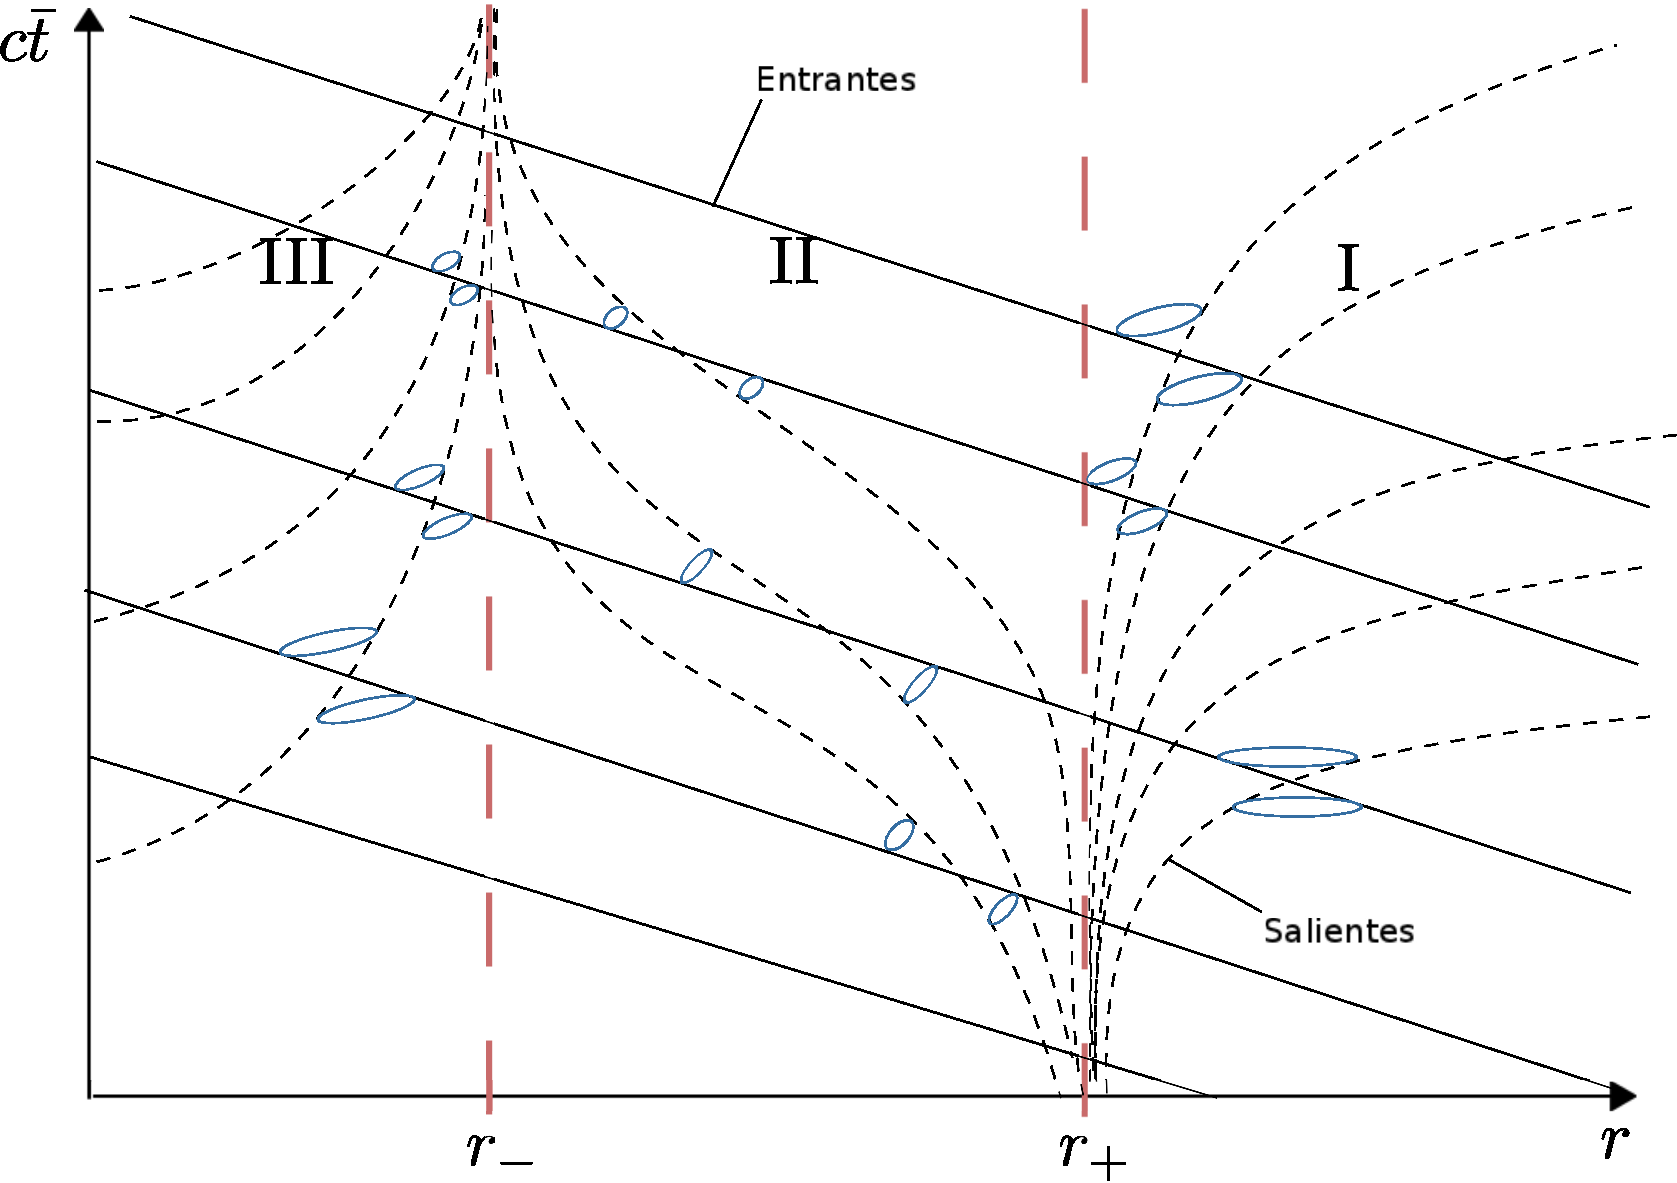
\includegraphics[height=6cm,angle=0]{fig/fig-conos2.pdf}
\caption{Diagrama de espacio tiempo en coordenadas de Eddington-Finkelstein.}
\label{fig:conos2}
\end{figure}

\subsection{L\'imite Estacionario y Observadores Estacionarios}

Al analizar la m\'etrica de Schwarzschild fue necesario utilizar observadores est\'aticos en el infinito, para estudiar la m\'etrica de Kerr se generaliza este concepto utilizando los llamados \textit{Observadores Estacionarios} que se eligen de tal forma que $r$ y $\theta$ permanezcan fijos
y que roten en torno al eje de giro del agujero negro con velocidad angular constante $\Omega$ dada por
\begin{equation}
\Omega=\frac{d\varphi}{dt}=c\frac{u^{\varphi}}{u^{0}},
\end{equation}
donde $u^{\mu}=dx^{\mu}/d\tau$ con $\tau$ el tiempo propio. Utilizando el hecho que el observador tiene una l\'inea de mundo tipo tiempo $(u^{\mu}u_{\mu}=c^2)$ entonces se debe cumplir que
\begin{equation}\label{cuadrados}
\left(u^{0}\right)^2\left[g_{\varphi \varphi}\frac{\Omega^2}{c^2}+2g_{\varphi 0}\frac{\Omega}{c} +g_{00}\right]=c^2, \qquad \theta=\frac{\pi}{2}.
\end{equation}

As\'i la expresi\'on entre corchetes cuadrados debe ser positiva. Debido  a que esa funci\'on tiene concavidad hacia abajo ($g_{\varphi \varphi}<0$), entonces 
\begin{equation}
\Omega_{-}<\Omega <\Omega_{+},
\end{equation}
donde $\Omega_{\pm}$ son la ra\'ices de la expresi\'on entre corchetes cuadrados en \eqref{cuadrados}
\begin{equation}\label{roots}
\Omega_{\pm}= c\left[ \frac{-g_{0\varphi}\mp\sqrt{g_{0\varphi}^2-g_{00}g_{\varphi \varphi}}}{g_{\varphi \varphi}} \right].
\end{equation}

Utilizando \eqref{BL2} notamos que $\Omega_{-}=0$ cuando $g_{00}=r^2-2mr+a^2\cos^2 \theta=0$, cuya soluci\'on (respetando que $r_+<r$) es justamente la superficie de redshift infinito $S_{+}$ que viene dada por el radio
\begin{equation}
r_{s_+}=m+\sqrt{m^2-a^2\cos^2\theta}.
\end{equation}

En el caso que $r_+<r<r_{s_+}$ la velocidad angular $\Omega$ siempre ser\'a postiva ya que en ese caso $\Omega_{-}>0$, que viene del hecho que $g_{00}>0$ (coordenada $ct$ es tipo tiempo). Por lo tanto, en este rango no pueden existir observadores est\'aticos (es decir con $\Omega=0$). As\'i, s\'olo en el caso en que $r=r_{s_+}$ se tiene que $\Omega=0$, raz\'on por la cual se le llama \textit{L\'imite Est\'atico}.\\

\begin{figure}[H]
\centering
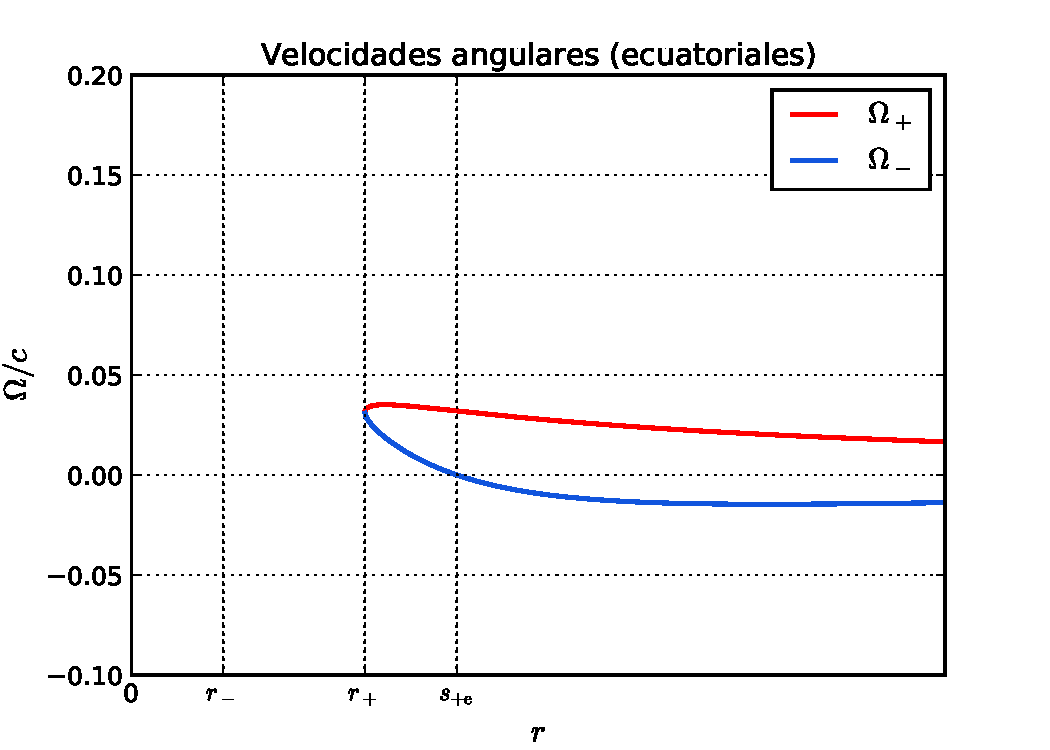
\includegraphics[height=7cm,angle=0]{fig/fig-omega-ecuatorial.pdf}
\caption{Frecuencias angulares permitidas para 'orbitas circulares ecuatoriales. C'odigo Python \href{https://github.com/gfrubi/GR/blob/master/figuras-editables/fig-omega-ecuatorial.py}{aqu\'i}.}
\label{fig:omegaecua}
\end{figure}

Adem'as, de \eqref{roots} se observa que los observadores estacionarios no existen si $g_{0\varphi}^2-g_{00}g_{\varphi \varphi}<0$, lo que se traduce en que $\Delta <0$, ya que
\begin{equation}
(r-r_-)(r-r_+)<0.
\end{equation}
As\'i, los observadores estacionarios existen s\'olo cuando $r>r_+$ que viene a ser la generalizaci\'on del hecho que los observadores est\'aticos no existen dentro del horizonte de eventos en la soluci\'on de Schwarzschild. Ver tambi'en la figura \ref{fig:omegaecua}.

%\subsubsection{Estructura de los Conos de Luz en la Erg\'osfera}
%
%Se consideran ahora curvas de part\'iculas tipo luz que tienen las coordenadas $r$ y $\theta$ fijas $(dr=d\theta=0)$ (no son geod\'esicas), es decir, part\'iculas que inicialmente estaban obligadas a orbitar la fuente con esta condici\'on de \eqref{BL} se obtiene que
%\begin{equation}
%\frac{\Delta}{\rho^2}(cdt-a\sen^2\theta d\varphi)^2-\frac{\sen^2\theta}{\rho^2}\left[(r^2+a^2)d\varphi-acdt \right]^2=0,
%\end{equation}
%
%de donde se tiene que 
%\begin{equation}\label{dphidt}
%\left( \frac{d\varphi}{dt} \right) _{\pm}=\frac{ac\sen \theta \pm c\sqrt{\Delta}}{(r^2+a^2)\sen\theta \pm a\sqrt{\Delta}\sen^2\theta}.
%\end{equation}
%
%En el caso de elegir la soluci\'on positiva en \eqref{dphidt} entonces  $d\varphi/dt >0$, con lo cual la part\'icula gira en el mismo sentido de la fuente. Ahora la pregunta es, para qu\'e caso  $d\varphi/dt \leqslant 0$, es decir, que la part\'icula gira en sentido contrario o parece estacionaria en estas coordenadas.\\
%
%Si se parte con la condici\'on $r> r_{+}$ en la soluci\'on negativa de \eqref{dphidt} se puede concluir f\'acilmente que el denominador de \eqref{dphidt} es positivo
%\begin{equation}
%(r^2+a^2)\sen\theta - a\sqrt{\Delta}\sen^2\theta >0.
%\end{equation}
%
%Luego, el sentido de rotaci\'on queda inmediatamente ligado al numerador de \eqref{dphidt}
%\begin{equation} \label{numerador}
%\frac{d\varphi}{dt}  \leqslant   0 \quad  \Leftrightarrow \quad  a\sen \theta - \sqrt{\Delta} \leqslant 0.
%\end{equation} 
%
%Desarrollando en \eqref{numerador} la condici\'on impuesta en el numerador, podemos escribir
%\begin{equation}
%\begin{aligned}
%a^2\sen^2 \theta &\leqslant \Delta ,\\
% a^2\sen^2 \theta &\leqslant r^2-2mr+a^2 , \\
% 0 &\leqslant r^2-2mr+a^2\cos^2 \theta ,\\
% 0 &\leqslant (r-r_{s_{+}})(r-r_{s_{-}}).\\
%\end{aligned}
%\end{equation}
%
%Como $r>r_{+}$ entonces $r>r_{s_-}$, luego la condici\'on buscada para que \eqref{dphidt} sea menor o igual que cero es que
%\begin{equation}
%r\geqslant r_{s_+}.
%\end{equation}
%
%Analizando este resultado, se tiene que si la part\'icula se encuentra sobre la superficie $S_+$, entonces \'esta parece estar estacionaria (para un observador estacionario en el infinito). En cambio m\'as all\'a de la supeficie dada, las part'iculas luminosas en el r\'egimen impuesto recorren las curvas en sentido inverso a la rotaci\'on de la fuente, no as\'i dentro de la erg\'osfera, donde las part\'iculas orientan su cono luz en la direcci\'on del giro de la fuente.\\

\section{Extracci\'on de Energ\'ia de una Agujero Negro Rotante}

\subsection{Geod\'esicas tipo tiempo}

En este caso se calcular\'an las geod\'esicas de part\'iculas en movimiento en el plano ecuatorial $\theta=\pi/2$. Para resolver el caso general se puede utilizar una forma descubierta por B. Carter\footnote{Brandon Carter (1942) f\'isico te\'orico australiano \url{http://en.wikipedia.org/wiki/Brandon_Carter}.}, que utiliza el m\'etodo de Hamilton-Jacobi.

Usaremos la funci\'on lagrangeana \eqref{lagrangeano1}, con $\dot{x}^{\mu}=dx^{\mu}/d \lambda$ y $\lambda$ es un par\'ametro af\'in que, por conveniencia, elegimos como $\lambda=\tau/m_0$, donde $m_0$ es la masa de la part\'icula movi\'endose en este campo gravitacional y $\tau$ su tiempo propio. Ya que el lagrangiano no depende expl'icitamente de las coordenadas $ct$ y $\varphi$, existen dos constantes de movimiento: $p^0=E/c$ y $p^\varphi=-L$, donde $E$ es la energ\'ia de la part\'icula y $L$ su momentum angular:
\begin{equation}
\begin{aligned}
p^{t}&:=\frac{\partial \bar{L}}{\partial(c\dot{t})}=\left(1-\frac{2m}{r}\right)c\dot{t}+\frac{2am\dot{\varphi}}{r}:=\frac{E}{c},\\ 
p^{\varphi}&:=\frac{\partial \bar{L}}{\partial \dot{\varphi}}=\frac{2am}{r}c\dot{t}-\left(r^2+a^2+\frac{2ma^2}{r}\right)\dot{\varphi}:=-L,\\
\end{aligned}
\end{equation}
y en general $p^\mu:=\partial\bar{L}/\partial\dot{x}^\mu$.

Despejando $c\dot{t}$ y $\dot{\varphi}$, de estas ecuaciones se obtiene que
\begin{equation}
\begin{aligned}
c\dot{t}&=\frac{(r^3+a^2r+2ma^2)E/c-2amL}{r\Delta},\\ \label{dottdotphi}
\dot{\varphi}&=\frac{(r-2m)L+2amE/c}{r\Delta}.\\
\end{aligned}
\end{equation}

De la identidad $g_{\mu \nu}p^{\mu} p^{\nu}=g_{\mu \nu}\dot{x}^{\mu}\dot{x}^{\nu}=m_0^2c^2$, se tiene que 
\begin{equation}\label{pp=m2c2}
\left[\left(1-\frac{2m}{r}\right)c^2\dot{t}^2-\frac{r^2}{\Delta}\dot{r}^2-\left(r^2+a^2+\frac{2ma^2}{r}\right)\dot{\varphi}^2
+\frac{4am}{r}\dot{\varphi}(c\dot{t}) \right]=m_0^2c^2,
\end{equation}
de donde podemos despejar $\dot{r}^2$:
\begin{equation}\label{dotr}
\frac{r^2}{\Delta}\dot{r}^2=\left(1-\frac{2m}{r}\right)c^2\dot{t}^2-\left(r^2+a^2+\frac{2ma^2}{r}\right)\dot{\varphi}^2
+\frac{4am}{r}\dot{\varphi}(c\dot{t}) -m_0^2c^2.
\end{equation}

Reemplazando \eqref{dottdotphi} en \eqref{dotr}, obtenemos
\begin{equation}
\frac{r^2}{\Delta}\dot{r}^2=\left( r^3+a^2r+2ma^2\right)\frac{E^2}{c^2r\Delta}-4am\frac{EL}{cr\Delta}-\left(r-2m\right)\frac{L^2}{r\Delta}-m_0^2c^2.
\end{equation}

Por lo tanto,
\begin{equation}\label{dotr2}
r^3\dot{r}^2=\left( r^3+a^2r+2ma^2\right)\frac{E^2}{c^2}-4am\frac{E}{c}L-\left(r-2m\right)L^2-m_0^2c^2r\Delta .
\end{equation}

Definimos la funci\'on
\begin{equation}\label{R}
R(E,L,r):=\left( r^3+a^2r+2ma^2\right)\frac{E^2}{c^2}-4am\frac{E}{c}L-\left(r-2m\right)L^2-m_0^2c^2r\Delta,
\end{equation}
de modo que \eqref{dotr2} adopta la forma:
\begin{equation}
r^3\left(\frac{dr}{d\lambda}\right)^2=R(E,L,r).
\end{equation}
De este modo, $R$ act'ua como un potencial unidimensional efectivo para nuestro problema.


Nos restringuimos ahora al caso en que la \'orbita de la part\'icula sea una circunsferencia, $\dot{r}=0$ y $\ddot{r}=0$, que entonces require que 
\begin{equation}
R=0, \qquad \frac{\partial R}{\partial r}=0.
\end{equation}
[\textbf{Tarea}: verifique la segunda condici'on, usando la ecuaci'on de la geod'esica]

Con estas condiciones se pueden encontrar los valores de $E$ y $L$ para el caso de una \'orbita circular:
\begin{equation}
\frac{E}{m_0c^2}=\frac{r^2-2mr\pm a\sqrt{mr}}{r\left(r^2-3mr\pm 2a\sqrt{mr}\right)^{\frac{1}{2}}} , \label{Ekerr}
\end{equation}

\begin{equation}
\frac{L}{m_0c}=\pm\frac{\sqrt{mr}\left(r^2\mp 2a\sqrt{mr}+a^2 \right)}{r\left(r^2-3mr\pm 2a\sqrt{mr}\right)^{\frac{1}{2}}} .\label{Lkerr} 
\end{equation}

El signo de arriba ($+$) al frente de \eqref{Lkerr} indica que la part\'icula gira en el mismo sentido que el agujero negro, en cambio con el de abajo $(-$) gira en sentido contrario al agujero (sentido retr\'ogrado).\\

Las \'orbitas circulares para part\'iculas con masa $m_0\neq 0$ existen desde el infinito hasta que la \'orbita circular anule el denominador de \eqref{Ekerr}--\eqref{Lkerr}\footnote{Esto equivale al caso de que las 'orbitas sean tipo luz, lo que se obtiene en el l'imite $L$ finito y $m_0\to 0$, de modo que $L/m_0\to\infty$.}. As\'i,
\begin{equation}
r^2_{\rm f}-3mr_{\rm f}\pm 2a\sqrt{mr_{\rm f}}=0,
\end{equation}
cuya soluci\'on puede escribirse como
\begin{equation}\label{phorbit}
r_{\rm f}=2m\left(1+\cos\left[\frac{2}{3}\cos^{-1}\left(\mp \frac{a}{m} \right) \right] \right).
\end{equation}

Donde $r_{\rm f}$ corresponde al radio de la \'orbita de un fot\'on en el plano ecuatorial. Cabe destacar que si $a=0$ entonces $r_{\rm f}=3m$, en cambio, si $a=m$ (rotaci\'on extrema) entonces $r_{\rm f}=m$ para 'orbitas que tienen el mismo sentido de la fuente y $r_{\rm f}=4m$ para \'orbitas retrogradas con respecto al sentido del giro de la fuente.\\

\begin{figure}[H]
\begin{center}
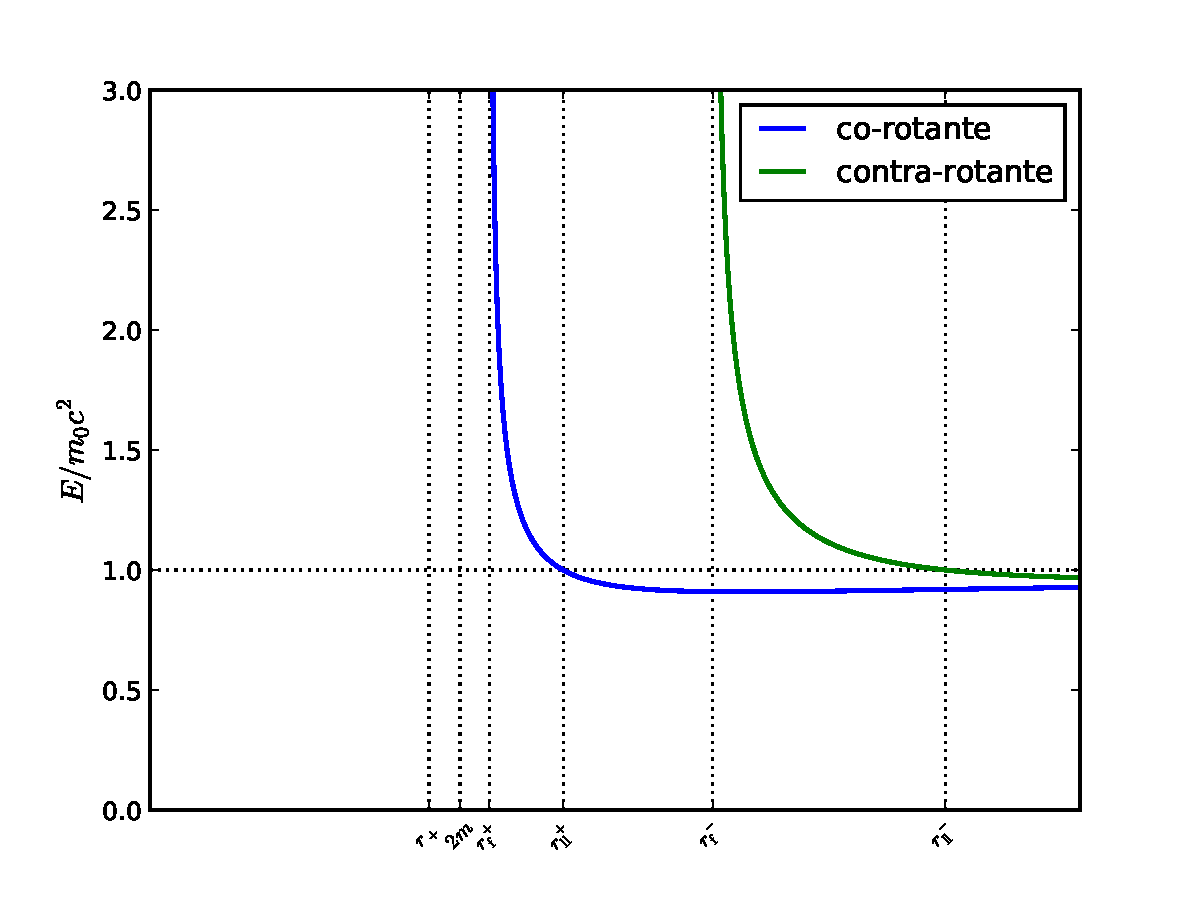
\includegraphics[height=7cm,angle=0]{fig/fig-Ecirc.pdf}
\caption{Energ'ias de 'orbitas circulares ecuatoriales, para $a=0.3m$.}
\label{fig:Ecirc}
\end{center}
\end{figure}

Se tiene que las \'orbitas con energ\'ia $E/m_0c^2>1$ son tales que bajo perturbaciones del radio las part\'iculas escapan al infinito con trayectoria hiperb\'olica y esto puede ocurrir perfectamente para $r>r_{\rm f}$. Luego los radios para los cuales las \'orbitas circulares son ligadas cumplen que $r>r_{\rm ll}$, donde $r_{\rm ll}$ es la \'orbita circular levemente ligada con energ\'ia $E/m_0c^2=1$, cuyo radio es
\begin{equation}\label{mborbit}
r_{ll}=2m\mp a+2\sqrt{m\left(m\mp a \right)}.
\end{equation}

Se tiene que si $a=0$ entonces $r_{\rm ll}=4m$ y para $a=m$, $r_{\rm ll}=m$ si la part\'icula gira en el mismo sentido que el agujero y $r_{\rm ll}=5.83m$ si la rotaci\'on es retrograda con respecto al agujero negro.\\

La estabilidad de la \'orbita estar\'a garantizada si $\partial^2 R/\partial r^2 \leq 0$. Utilizando \eqref{R} tenemos que
\begin{equation}
\frac{\partial^2 R}{\partial r^2}=6r\frac{E^2}{c^2}-m_0^2c^2\left(6r-4m\right) \leq 0.
\end{equation}

Luego
\begin{equation}\label{stable}
1-\frac{E^2}{m_0^2c^4} \leq \frac{2m}{3r}.
\end{equation}

Reemplazando \eqref{Ekerr} en \eqref{stable} obtenemos
\begin{equation}
r^2-6mr\pm 8a\sqrt{mr}-3a^2 \geq 0.
\end{equation}

As\'i, se encuentra la siguiente condici\'on para el radio de la \'orbita :
\begin{equation}
r \geq r_{\rm le}.
\end{equation}

Aqu\'i $r_{\rm le}$ es el radio de la \'orbita circular levemente estable la cual est\'a dada por
\begin{equation}
r_{\rm le}=m\left[ 3+Z_2\mp \sqrt{\left(3-Z_1\right)\left( 3+Z_1+2Z_2\right)}\right],
\end{equation}

donde
\begin{eqnarray}
&Z_1=1+\left( 1-\frac{a^2}{m^2}\right)^{\frac{1}{3}}\left[\left( 1+\frac{a}{m}\right)^{\frac{1}{3}}+\left( 1-\frac{a}{m}\right)^{\frac{1}{3}} \right] ,\\
&Z_2 =\left(\frac{3a^2}{m^2}+Z_1^2 \right)^{\frac{1}{2}}.
\end{eqnarray}

Se tiene que para $a=0$, entonces $r_{\rm le}=6m$ y para $a=m$, $r_{\rm le}=m$ si la part\'icula gira en la misma direcci\'on que el agujero negro y $r_{\rm le}=9m$ si la part\'icula gira en sentido retr\'ogrado con respecto al agujero.\\

%Se tiene que en este sistema de coordenadas los radios caracter\'isticos son $r_{\rm le}=r_{\rm ll}=r_{\rm f}=r_{+}=m$ en el caso que $a \rightarrow m$, pero se puede demostrar que la \'orbita $r_{\rm le}$ est\'a siempre causalmente desconectada (curva tipo espacio) de las otras. Esto se hace calculando la distancia propia $s$ entre dos puntos dados por $x^{\mu}_{1}=(ct_0,r_{1},\theta_0,\varphi_0)$ y $x^{\mu}_2=(ct_0,r_2,\theta_0,\varphi_0)$ en el l\'imite dado. As\'i, de \eqref{BL2} se tiene que
%\begin{equation}\label{propdist}
%\begin{aligned}
%s&=\lim_{a \rightarrow m}\int_{x^{\mu}_1}^{x^{\mu}_2}\sqrt{|ds^2|}\\
%&=\lim_{a \rightarrow m}\int_{r_1}^{r_2} \frac{rdr}{\sqrt{r^2-2mr+a^2}}.
%\end{aligned}
%\end{equation}
%
% \begin{figure}[H]
% \centering
%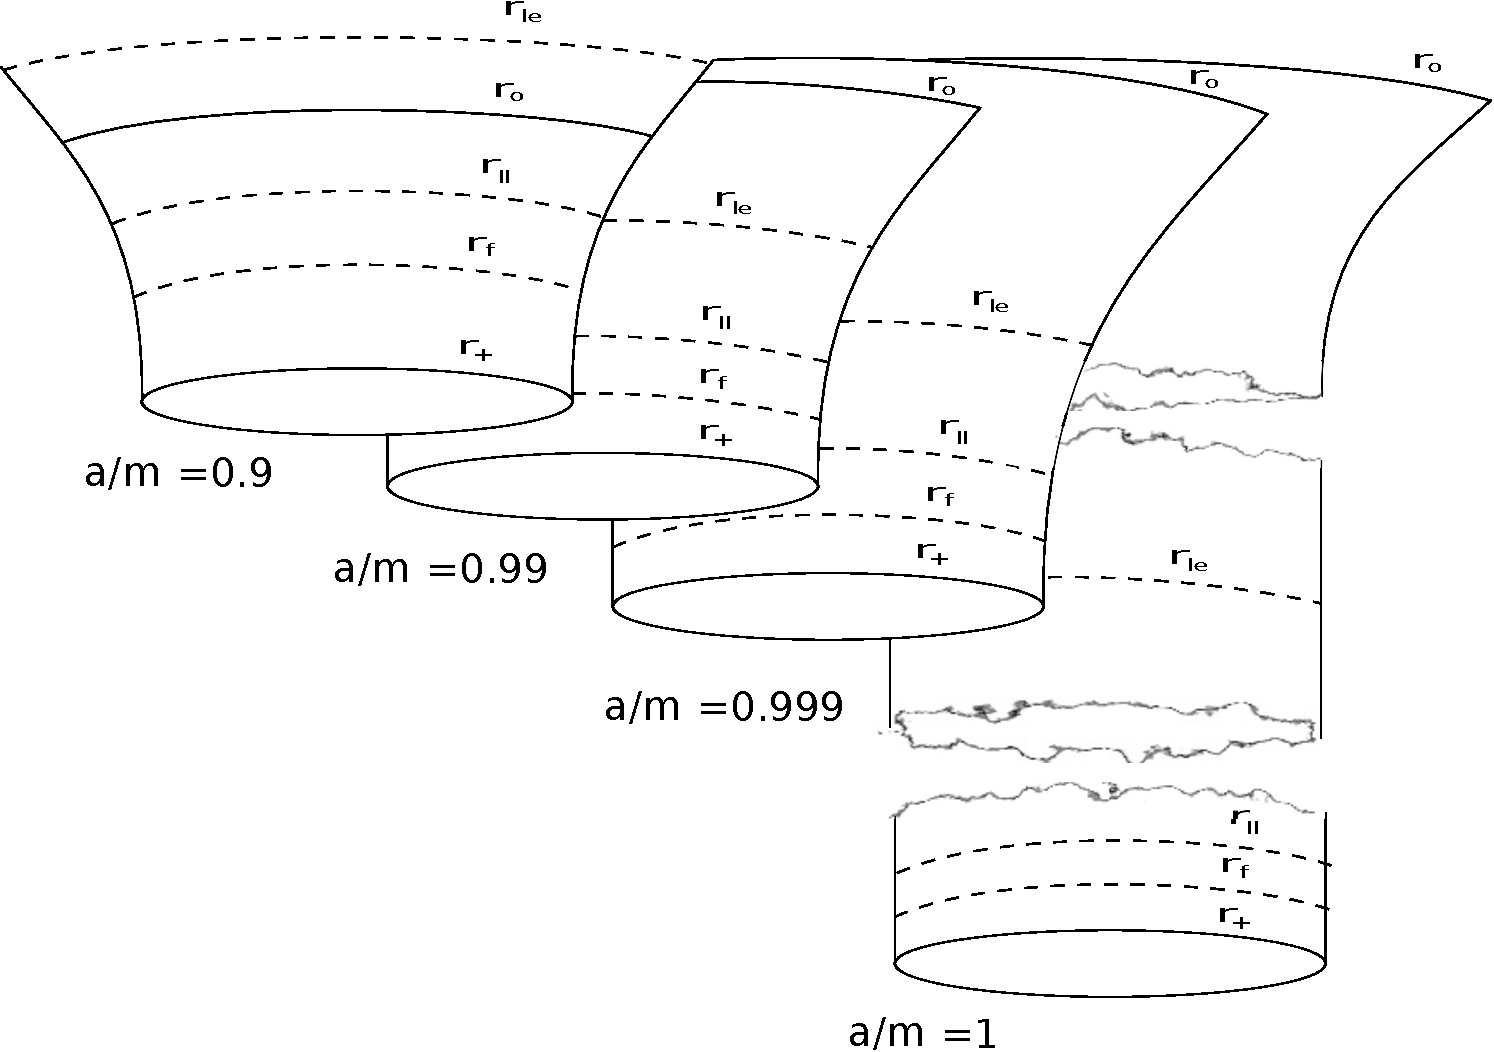
\includegraphics[height=8cm,angle=0]{fig-embedding.pdf}
%\caption{Representaci\'on de la conexi\'on causal entre \'orbitas a medida de que aumenta la velocidad angular.}
%\label{fig:tubos}
%\end{figure}


Se encuentra que \eqref{propdist} diverge cuando $r_1=r_{\rm le}$ y $r_{\rm f}=r_{\rm +}=r_{0}=r_{\rm ll}=r_{\rm f}$. Esto significa que no hay conexi\'on causal entre estos radios cuando el agujero negro es maximalmente rotante (ver figura \ref{fig:tubos}).

\subsubsection{Energ\'ia de Enlace}

La energ\'ia de enlace $E_{\rm e}$ se define como la energ\'ia necesaria para tomar la part\'icula y ponerla en el infinito (part\'icula libre con energ\'ia $E=m_0c^2$). Por lo tanto, la energ\'ia de enlace para una part\'icula de energ\'ia $E$ y masa en reposo $m_0$ es
 \begin{equation}
 \begin{aligned}
 E_{\rm e}&=E_{\rm f}-E_{\rm i}\\
 &=m_0c^2\left(1-\frac{E}{m_0c^2}\right).
 \end{aligned}
 \end{equation}
 
Para el estudio de la energ\'ia de enlace de una \'orbita circular levemente estable es conveniente reemplazar  \eqref{stable} (en el caso de la igualdad) en \eqref{Ekerr}, con lo cual se obtiene la siguiente relaci\'on
\begin{equation}
\frac{a}{m}=\mp\frac{4\sqrt{2}\left(1-\frac{E^2}{m_0^2c^4} \right)^{1/2}-\frac{2E}{m_0c^2}}{3\sqrt{3}\left(1-\frac{E^2}{m_0^2c^4} \right)}.
\end{equation}

As\'i, para part\'iculas que giran en la misma direcci\'on de giro que el agujero negro la energ\'ia decrece desde $E=(2\sqrt{2}/3)m_0c^2$ para $a=0$ hasta $E=(1/\sqrt{3})m_0c^2$ para $a=m$.\\

Para part\'iculas que giran en un sentido retr\'ogrado la energ\'ia crece desde $E=(2\sqrt{2}/3)m_0c^2$ para $a=0$ hasta $E=(5/3\sqrt{3})m_0c^2$ para $a=m$.\\

El m\'aximo valor de la energ\'ia de enlace se alcanza cuando el agujero negro es maximalmente rotante y la part\'icula gira en sentido directo, cuyo valor es $E_{\rm e}=(1-1/\sqrt{3})m_0c^2 \approx 0.423 m_0c^2$, es decir, un 42,3$\%$ de la energ\'ia en reposo de la part\'icula. Esta energ\'ia de enlace es la energ\'ia que libera la part\'icula al momento girar hacia al agujero negro a trav\'es de una serie de \'orbitas circulares. Luego, como esta energ\'ia se liber\'o en el agujero (qued\'o en aquel lugar) se puede considerar al agujero negro como una fuente de energ\'ia. Luego de pasar la \'orbita circular levemente estable, la part\'icula libera muy poca energ\'ia hasta caer dentro del agujero negro.\\

\subsection{Regi\'on de Energ\'ia Negativa}

Resolviendo la ecuaci\'on \eqref{dotr2} para $E$, se obtiene la siguiente expresi\'on:
\begin{equation}\label{energia}
\frac{E}{c}=\frac{2amL+\sqrt{L^2r^2\Delta+\left(r^3+a^2r+2ma^2\right)\left(m_0^2c^2r\Delta+\dot{r}^2r^3\right)}}{r^3+a^2r+2ma^2}.
\end{equation}

Cabe destacar la elecci\'on del signo postivo antes de la ra\'iz de \eqref{energia}, ya que en este caso al hacer $r\rightarrow \infty$ la energ\'ia es postiva ($E \geq m_0c^2$). En el caso de que $E<0$ se requiere que $L<0$ (\'orbita retr\'ograda) como se observa en \eqref{energia}, con la condici\'on de que el valor absoluto de la primera parte en el numerador de esta expresi\'on sea mayor que el valor absoluto de la segunda, o equivalentemente:
\begin{equation}\label{desigualdad}
L^2r^2\Delta+\left(r^3+a^2r+2ma^2\right)\left(m_0^2c^2r\Delta+\dot{r}^2r^3\right) < 4a^2m^2L^2.
\end{equation}

De \eqref{desigualdad}, se tiene que
\begin{equation}\label{desigualdad2}
r^2 \Delta +\left(r^3+a^2r+2ma^2\right)\left(\frac{m_0^2}{L^2}c^2r\Delta+\frac{\dot{r}^2}{L^2}r^3\right) < 4a^2m^2.
\end{equation}

Para obtener el l\'imite de la regi\'on con energ\'ia negativa se debe hacer que la parte izquierda de \eqref{desigualdad2} s\'olo tenga dependencia en la parte radial tal que $r$ tenga su mayor valor posible y se respete la desigualdad. Para lo cual se debe tener que $L>>m_0ca$ y $\dot{r} \rightarrow 0$, as\'i
\begin{equation}\label{desigualdad3}
r^2 \Delta < 4a^2m^2,
\end{equation}
donde se obtiene que el radio m\'aximo permitido es $r=r_0=2m$, es decir, el l\'imite estacionario en el plano ecuatorial. Por lo tanto las part\'iculas con energ\'ia negativa se encuentran en \'orbitas inferiores al l\'imite estacionario.\\

\subsection{Mecanismo de Penrose}

Sir Roger Penrose y R. M. Floyd explotaron  la existencia de energ\'ia negativa en un trabajo publicado en 1971 [42], donde explica c\'omo extraer energ\'ia de un agujero negro rotante, es decir, utilizar estos colosos como fuente de energ\'ia. El mec\'anismo que lleva su nombre se demuestra con el siguiente experimento pensado. Dada una part\'icula con una determinada energ\'ia $E_{\rm en}$ y una trayectoria tal que pase el l\'imite estacionario y considere que cuando se encuentre en la erg\'osfera ($r_+<r<r_0$) se divida en dos part\'iculas, una que sea capaz de salir de la erg\'osfera hacia al infinito, con una energ\'ia $E_{\rm sal}$, y otra part\'icula que tenga energ\'ia $E$ que luego sea absorbida por el agujero (que entre en el horizonte de eventos). Utilizando la conservaci\'on de energ\'ia,
\begin{equation}
E_{\rm en}=E_{\rm sal}+E,
\end{equation}
en el caso que $E<0$ se tiene que $E_{\rm sal}>E_{\rm en}$. As\'i, el hecho de existir \'orbitas en una regi\'on determinada (erg\'osfera) con energ\'ia negativa abre la posibilidad de que una part\'icula que sea observida por el agujero negro eyecte al infinito otra una energ\'ia a\'u mayor.\\

La energ\'ia con la cual sale la part\'icula es extraida de la energ\'ia rotacional del agujero negro, la cu\'al disminuye al momento que la par\'icula con energ\'ia negativa que tiene por supuesto una \'orbita retr\'ograda, es capturada.\\

De la misma forma en las ondas (electromagn\'eticas o gravitacionales) ocurre un fen\'omeno similar de amplificaci\'on de la energ\'ia donde, con un valor de la frecuencia adecuado estas ondas son dispersadas por el agujero negro rotante. Parte de la onda es absorbida y otra parte es emitida con energ\'ia mayor que la incidente. A este fen\'omeno se le llama Super Radiancia.\\

\subsubsection{L\'imite Inferior de la Velocidad Relativa}

James Maxwell Bardeen et al. en su trabajo de 1972 [43] mostraron que existe un l\'imite inferior para la velocidad relativa entre las part\'iculas (creadas de la separaci\'on de la part\'icula entrante) que se encuentran en la erg\'osfera del agujero negro para que se lleve a cabo el mecanismo de Penrose.\\

Se considera una part\'icula de masa $m_0$ y una cantidad conservada $E=cp_{\mu}\xi_{(t)}^{\mu}$ a lo largo de la geod\'esica, que se identifica con la energ\'ia, donde $\xi_{(t)}^{\mu}=(1,0,0,0)$ es el vector de Killing temporal (vector asociado a la simetr\'ia en la direcci\'on temporal de la soluci\'on de Kerr) y $p^{\mu}=m_0 u^{\mu}$ es el 4-momentum. Lo primero que se har\'a ser\'a encontrar cu\'al es rango de energ\'ia de la cantidad $E/m_0c^2$ para un punto del espacio-tiempo en general.\\

Escogiendo una tetrada ortonormal $\left(e^{\mu}_a\right)_{a=1,4}$ como base  para expresar la 4-velocidad y el vector de Killing temporal en un punto determinado, se tiene que
\begin{equation}\label{uyxi}
u^a=u^{\mu}e^a_{\mu}=(\gamma c, \gamma \vec{v}), \qquad \xi^a_{(t)}=\xi^{\mu}_{(t)}e^a_{\mu}=\left(\xi^{\hat{0}},\vec{\xi} \right).
\end{equation}
donde se satisface que $g_{\mu \nu}=\eta_{ab}e^a_{\mu}e^b_{\nu}$ con $g_{\mu \nu}$ la m\'etrica de Kerr y $\eta_{ab}$ la m\'etrica de Minkowski, donde adem\'as $\vec{v}$ es el vector velocidad de la part\'icula, $\gamma=1/\sqrt{1-\frac{v^2}{c^2}}$ y $\vec{\xi}$ es un vector en el espacio 3-dimensional.\\

De \eqref{uyxi}, el cuociente entre la energ\'ia de la part\'icula y su energ\'ia en reposo es
\begin{equation}\label{E/mu}
\frac{E}{m_0c^2}=\frac{g_{\mu \nu}u^{\mu}\xi_{(t)}^{\nu}}{c}=\frac{\eta_{ab}u^a\xi^b_{(t)}}{c}=\gamma\left(\xi^{\hat{0}}-\frac{\vec{v} \cdot \vec{\xi}}{c} \right)
\end{equation}

Una condici\'on necesaria para que \eqref{E/mu} sea un extremo es que $\vec{v}$ y $\vec{\xi}$ sean (anti)paralelos, de modo que $\vec{v} \cdot \vec{\xi}=\pm v\xi$ con $\xi=\sqrt{\vec{\xi}\cdot \vec{\xi}}$. Adem\'as, se tiene que
\begin{equation}\label{xi2}
\xi_{(t)}^2=g_{\mu \nu} \xi_{(t)}^{\mu}\xi_{(t)}^{\nu}=g_{00}=\left( 1-\frac{2mr}{\rho^2}\right)
\end{equation}
donde el valor de la norma del 4-vector es un escalar, con lo cual es independiente de las coordenadas utilizadas, en particular al utilizar las coordenadas de Kerr se obtiene \eqref{xi2}.\\

Por lo tanto, si la part\'icula se encuentra en la erg\'osfera entonces $\xi_{(t)}^{\mu}$ es un vector tipo espacio, que significa que $\xi^2_{(t)}<0$ entonces $\xi_{\hat{0}}^2-\xi^{2}<0$, con lo cual $\xi^{\hat{0}} < \xi$. As\'i, de \eqref{E/mu} se ve que todos los valores son permitidos para $E/m_0c^2$, donde el l\'imite superior se da con $v \rightarrow c$ y $\vec{v} \cdot \vec{\xi}=-v\xi$ y el inferior tambi\'en con $v \rightarrow c$ y $\vec{v} \cdot \vec{\xi}=+v\xi$. Por lo tanto,
\begin{equation}\label{condicion1}
-\infty <\frac{E}{m_0c^2}<+\infty.
\end{equation}

En el caso de estar fuera de la erg\'osfera de \eqref{xi2} se tiene que $\xi_t^{\mu}$ es tipo tiempo, con lo cual $\xi^{\hat{0}} >\xi$. Con esto el valor de la energ\'ia es siempre positivo, donde se debe determinar el l\'imite inferior del rango permitido para el couciente \eqref{E/mu}.\\

Derivando la expresi\'on \eqref{E/mu} con respecto a $v$ e igualandola a 0, se encuentra que el valor de la velocidad que extremiza el valor de la energ\'ia es:
\begin{equation}\label{v}
v=\frac{c\xi}{\xi^{\hat{0}}}.
\end{equation}

Reemplazado \eqref{v} en \eqref{E/mu}, se obtiene que el l\'imite inferior viene dado por la norma del m\'odulo del vector de Killing en el caso que es tipo tiempo $\xi_{(t)}$ (donde $\xi^2_{(t)}=\xi_{\hat{0}}^2-\xi^2$) :
\begin{equation}\label{condicion2}
\xi_{(t)}\leq  \frac{E}{m_0c^2}<+\infty.
\end{equation}

Como \eqref{condicion2} est\'a dentro del rango \eqref{condicion1}, entonces se encuentra la condici\'on general
\begin{equation}
\frac{E^{2}}{m_0^2c^4}-\xi_{(t)}^2 \geq 0.
\end{equation}

Para encontrar el l\'imite inferior para la velocidad, se debe considerar lo siguiente: Dada las \'orbitas de dos part\'iculas de masa $m_1$ y $m_2$ que se intersectan en un punto, donde las energ\'ias de cada part\'icula son $E_1$ y $E_2$, respectivamente, y con diferentes 4-velocidades, tal que la norma vector de velocidad relativo $|w|$ (velocidad de una part\'icula vista por un observador com\'ovil con la otra part\'icula) es distinto de cero.\\

Se escoge nuevamente una tetrada ortonormal como base de los 4-vectores en este punto, tal que las correspondientes 4-velocidades son
\begin{equation}
u_1^{a}=\left(\gamma c, -\gamma \vec{v} \right), \qquad u_2^{a}=\left(\gamma c, \gamma \vec{v}\right).
\end{equation}

La magnitud de la velocidad relativa $|w|$, se encuentra utilizando la f\'ormula de composici\'on de velocidades:
\begin{equation}\label{w}
|w|=\frac{2v}{1+\frac{v^2}{c^2}}.
\end{equation}

Adem\'as, de \eqref{E/mu} se tiene que
\begin{equation}\label{sistema}
\frac{E_1}{m_1c^2}=\gamma\left(\xi^{\hat{0}}+\frac{\vec{v} \cdot \vec{\xi}}{c} \right), \qquad \frac{E_2}{m_2c^2}=\gamma\left(\xi^{\hat{0}}-\frac{\vec{v} \cdot \vec{\xi}}{c} \right).
\end{equation}

Resolviendo el sistema de ecuaciones \eqref{sistema} para $\xi_{\hat{0}}^2$ y $\xi^2$, considerando que $\vec{v}\cdot \vec{\xi} \equiv v\xi \cos \eta$, donde $\eta$ es el \'angulo entre $\vec{v}$ y $\vec{\xi}$, se tiene que
\begin{equation}
\begin{aligned}
\xi_{\hat{0}}^2&=\frac{\left(\frac{E_1}{m_1c^2}+\frac{E_2}{m_2c^2} \right)^2}{4\gamma ^2},\\
\xi^2&=\frac{\left(\frac{E_1}{m_1c^2}-\frac{E_2}{m_2c^2} \right)^2}{4\frac{\gamma ^2 v^2}{c^2}\cos^2 \eta}. \\
\end{aligned}
\end{equation}

Con lo cual se tiene que
\begin{equation}
\left(\frac{E_1}{m_1c^2}-\frac{E_2}{m_2c^2} \right)^2=\left[\left(\frac{E_1}{m_1c^2}+\frac{E_2}{m_2c^2}\right)^2-4\gamma^2 \xi_{(t)}^2   \right]\frac{v^2}{c^2}\cos^2 \eta.
\end{equation}

Utilizando el hecho que $0\leq |\cos \eta| \leq 1$ se tiene que
\begin{equation}
\left(\frac{E_1}{m_1c^2}-\frac{E_2}{m_2c^2} \right)^2 \leq \left[\left(\frac{E_1}{m_1c^2}+\frac{E_2}{m_2c^2} \right)^2-4\gamma^2 \xi_{(t)}^2 \right]\frac{v^2}{c^2}.
\end{equation}

Resolviendo la \'ultima desigualdad para $v/c$ se tiene que
\begin{equation}\label{v/c}
\frac{v^2}{c^2} \geq \left[ \frac{\frac{E_1}{m_1c^2} -\frac{E_2}{m_2c^2}}{\sqrt{\frac{E_1^2}{m_{1}^{2}c^{4}}-\xi_{(t)}^2}+\sqrt{ \frac{E_2^2}{m_{2}^{2}c^{4}} -\xi_{(t)}^2}}\right]^2 .
\end{equation}

Aplicando las relaciones encontradas al caso de tener la geometr\'ia de Kerr, de \eqref{xi2} con $r \geq r_+$, encontramos
\begin{equation}
|\xi_{(t)}^2| \leq 1, \qquad  \forall \quad \theta,\varphi .
\end{equation}

Sea $E_1$ el valor de la m\'inima energ\'ia de una part\'icula que se encuentra en el m\'inimo radio en que la \'orbita circular es estable, la cual se da cuando $a \rightarrow m$ y $E_2$ tiene el valor de la energ\'ia de una part\'icula que se encuentra en el borde de la regi\'on de energ\'ia negativa
\begin{equation}
\frac{E_1}{m_1c^2}=\frac{1}{\sqrt{3}}, \qquad \frac{E_2}{m_2c^2}=0.
\end{equation}

De \eqref{v/c} se obtiene que
\begin{equation}\label{finalv/c}
\frac{v}{c} \geq 2-\sqrt{3}.
\end{equation}

Y finalmente, reemplazando \eqref{finalv/c} en \eqref{w}, se obtiene la siguiente desigualdad
\begin{equation}
|w|\geq \frac{c}{2}.
\end{equation}

As\'i, para lograr extraer energ\'ia de un agujero negro rotante la part\'icula que es capaz de salir debe acelerar a una velocidad tal que la velocidad relativa sea al menos la mitad de la velocidad de la luz, ya que bajo este requerimiento existir\'a una part\'icula en la regi\'on de energ\'ia negativa, logrando salir la part\'icula que se encuentra fuera de esta regi\'on (de energ\'ia negativa) con m\'as energ\'ia que la part\'icula entrante.\\


\chapter{Campos gravitacionales d'ebiles y ondas gravitacionales}\label{capdebil1}

\section{Expansi'on en potencias de \texorpdfstring{$G$}{G}}
Las ecuaciones de Einstein son no-lineales en la m'etrica. Por esto, sus
soluciones dependen de forma nolineal del tensor de energ'ia-momentum de la
materia (que asumimos conocido). Como $T^{\mu\nu}$ aparece al lado derecho de las ecuaciones de Einstein siempre multiplicado por la constante de gravitaci'on $G$, es decir, en la combinaci'on $GT^{\mu\nu}$, entonces las componentes m'etricas depender'an no-linealmente de $G$. Podemos verificar esta propiedad, por ejemplo, en el caso de la soluci'on de Schwarzschild.

Asumiendo que el \textit{campo gravitacional es d'ebil} (curvatura peque\~na), pero \textit{no necesariamente estacionario}, es posible desarrollar un \textit{m'etodo perturbativo}
para expresar las soluciones de las ecuaciones de Einstein como una serie de
t'erminos, cada uno proporcional a una potencia dada de la constante de gravitaci'on $G$.

%Aqu'i consideraremos s'olo la aproximaci'on a primer orden.
% Adem'as las velocidades de
% las part'iculas no necesitan ser peque\~nas comparadas con la velocidad de la
% luz.

Dividimos la m'etrica en
\begin{equation} \label{exp01}
g_{\mu\nu}=\eta_{\mu\nu}+h_{\mu\nu}, \qquad \left|h_{\mu\nu}\right|<< 1,
\end{equation}
donde $\eta$ es la m'etrica plana, es decir, $Riemann(\eta)=0$ y usaremos
coordenadas ``cuasi-inerciales'' $x^\mu$ tales
que $\eta_{\mu\nu}=diag(+1,-1,-1,-1)$. Adem'as, separaremos la perturbaci'on $h_{\mu\nu}$ en una serie de potencias de $G$, de modo que
\begin{equation}
h_{\mu\nu}=h^{(1)}_{\mu\nu}+h^{(2)}_{\mu\nu}+h^{(3)}_{\mu\nu}+\cdots,
\end{equation}
donde $h^{(n)}_{\mu\nu}$, $n=0,1,\cdots$, denota el t'ermino proporcional a $G^n$. En particular $h^{(0)}_{\mu\nu}=\eta_{\mu\nu}$.

%Nos concentraremos en el t'ermino de primer orden, de modo que
% consideraremos que $h_{\mu\nu}$ es lineal en $G$, lo que denotamos por
% $h=\mathcal{O}(G)$.

% Recuerde que en el sistema solar
% $\left|h_{\mu\nu}\right|\sim \frac{|\phi|}{c^2} \sim
% \frac{GM_\odot}{c^2R_\odot} \sim 10^{-6}$.

Realizaremos una expansi'on similar para cada cantidad relevante. Por ejemplo,
\begin{align}
\Gamma^\lambda_{\mu\nu} &= \Gamma^{\lambda}_{(1)\mu\nu}+\Gamma^{\lambda}_{(2)\mu\nu}+\Gamma^{\lambda}_{(3)\mu\nu}+\cdots, \\
R_{\mu\nu} &= R^{(1)}_{\mu\nu}+R^{(2)}_{\mu\nu}+R^{(3)}_{\mu\nu}+\cdots,\\
G_{\mu\nu} &= G^{(1)}_{\mu\nu}+G^{(2)}_{\mu\nu}+G^{(3)}_{\mu\nu}+\cdots.
\end{align}
Note que, ya que el t'ermino de orden cero es la m'etrica plana (y adem'as usamos coordenadas donde esta m'etrica plana es constante), las expansiones de la conexi'on, curvatura, y el tensor de Einstein comienzan con el orden 1.

Similarmente, es necesario en general considerar una expansi'on del tensor de energ'ia-momentum de la materia:
\begin{equation}
T_{\mu\nu}=T^{(0)}_{\mu\nu}+T^{(1)}_{\mu\nu}+T^{(2)}_{\mu\nu}+\cdots.
\end{equation}
Aqu'i $T_{\mu\nu}^{(0)}$ representa el tensor de energ'ia-momentum de la materia a orden cero en $G$, \textbf{como si la materia estuviese distribuida en un espacio plano}. Recuerde que en general $T_{\mu\nu}$ depende de la m'etrica\footnote{Por ejemplo, para un fluido perfecto $T^{\mu\nu}=(\rho+p/c^2) u^\mu u^\nu-p\,g^{\mu\nu}$.}, por lo que es necesario realizar la expansi'on correspondiente para $T_{\mu\nu}$.

Con esto, las ecuaciones de Einstein adoptan la forma
\begin{equation}
G^{(1)}_{\mu\nu}+G^{(2)}_{\mu\nu}+G^{(3)}_{\mu\nu}+\cdots=
\frac{8\pi G}{c^4}\left(T^{(0)}_{\mu\nu}+T^{(1)}_{\mu\nu}+T^{(2)}_{\mu\nu}+\cdots\right),
\end{equation}
que \textit{separaremos}, consistentemente, en
\begin{align}
G^{(1)}_{\mu\nu}&=\frac{8\pi G}{c^4}T^{(0)}_{\mu\nu},\label{orden1}\\
G^{(2)}_{\mu\nu}&=\frac{8\pi G}{c^4}T^{(1)}_{\mu\nu},\\
G^{(3)}_{\mu\nu}&=\frac{8\pi G}{c^4}T^{(2)}_{\mu\nu}\label{orden3},
\end{align}
etc.

\subsection{Expansi'on a primer orden}
\subsubsection{M'etrica}

Primero requerimos calcular la m'etrica inversa $g^{\mu\nu}$
\begin{equation}
g^{\mu\nu}=\eta^{\mu\nu}+g^{\mu\nu}_{(1)}+g^{\mu\nu}_{(2)}+\mathcal{O}(G^3).
\end{equation}
Un c'alculo simple muestra que
\begin{align}
g^{\mu\nu}_{(1)}&=-\eta^{\mu\lambda}\eta^{\nu\rho}h_{\lambda\rho}=:-h^{\mu\nu}_{(1)} .
\end{align}

\textit{Por convenci'on, en el contexto de la expansi'on realizada subimos y bajamos los 'indices usando la m'etrica plana} $\eta$. As'i, por ejemplo, $h^{(1)}:=h^\mu_{(1)}{}_\mu=\eta^{\mu\nu}h^{(1)}_{\mu\nu}$ es la \textit{traza} del tensor $h^{(1)}_{\mu\nu}$ y $\square :=\partial_\mu\partial^\mu=\eta^{\mu\nu}\partial_\mu\partial_\nu$ es el operador de onda.
\subsubsection{Conexi'on}\label{sec:conG1}

La primera contribuci'on a los s'imbolos de Christoffel resultan ser
\begin{align}
\Gamma^\lambda_{(1)\mu\nu}&=\frac{1}2\eta^{\lambda\rho}\left(\partial_\mu
h^{(1)}_{\nu\rho} +\partial_\nu h^{(1)}_{\mu\rho} - \partial_\rho h^{(1)}_{\mu\nu}\right)\\
&=\frac{1}{2}\left(\partial_\mu h^\lambda_{(1)\nu} + \partial_\nu h^\lambda_{(1)\mu} -\partial^\lambda h^{(1)}_{\mu\nu}\right) . \label{Gamma1}
\end{align}

\subsubsection{Tensor de curvatura de Riemann}
Similarmente, el t'ermino de primer orden del tensor de curvatura es:
\begin{align}
R^\rho_{(1)\mu\nu\lambda}&= \partial_\nu
\Gamma^\rho_{(1)\mu\lambda}-\partial_\lambda \Gamma^\rho_{(1)\mu\nu} \\
&= \frac{1}{2}\left(\partial_\mu\partial_\nu h^\rho_{(1)\lambda} -
\partial_\mu\partial_\lambda h^\rho_{(1)\nu} + \partial_\lambda \partial^\rho
h^{(1)}_{\mu\nu} - \partial_\nu\partial^\rho h^{(1)}_{\mu\lambda}\right)  \, .
\end{align}

\subsubsection{Tensor de Ricci}

Como consecuencia, el tensor de Ricci es de la forma:
\begin{align}
R^{(1)}_{\mu\lambda}&=R^\rho_{(1)\mu\rho\lambda} \\
&=\frac{1}{2}\left(\partial_\mu\partial_\nu h^\nu_{(1)\lambda}
 + \partial_\lambda \partial^\nu h^{(1)}_{\mu\nu}- \partial_\mu\partial_\lambda h^{(1)} -\square h^{(1)}_{\mu\lambda}\right).
\end{align}




\subsubsection{Escalar de Curvatura}

El escalar de curvatura es dado, a primer orden por,
\begin{equation}\label{R1}
R^{(1)}=\eta^{\mu\nu}R^{(1)}_{\mu\nu}=\partial^\mu\partial^\nu h^{(1)}_{\mu\nu} - \square h^{(1)} .
\end{equation}


\subsubsection{Tensor de Einstein}

Finalmente, el tensor de Einstein es
\begin{align}
G^{(1)}_{\mu\nu} &= R^{(1)}_{\mu\nu}-\frac{1}{2}\eta_{\mu\nu}R^{(1)}\\
&= \frac{1}{2}\left[\partial_\mu\partial^\lambda h^{(1)}_{\lambda\nu} +\partial_\nu\partial^\lambda h^{(1)}_{\lambda\mu} - \partial_\mu\partial_\nu h^{(1)} -\square h^{(1)}_{\mu\nu} -\eta_{\mu\nu}\left(\partial^\lambda \partial^\rho h^{(1)}_{\lambda\rho} - \square h^{(1)}\right) \right].
\end{align}
Es conveniente definir el tensor $\bar{t}_{\mu\nu}$, asociado a un
tensor sim'etrico $t_{\mu\nu}$, como
\begin{eqnarray}
\bar{t}_{\mu\nu}&:=&t_{\mu\nu}-\frac{1}2\eta_{\mu\nu}\, t \label{tbarra}\\
&=&t_{\mu\nu}-\frac{1}2\eta_{\mu\nu}\, \eta^{\lambda\rho}\, t_{\lambda\rho} \, .
\end{eqnarray}
Puede verificarse que 
\begin{equation}
\bar{t}:= \eta^{\mu\nu}\,\bar{t}_{\mu\nu}=-t, \qquad 
\bar{\bar{t}}_{\mu\nu}=t_{\mu\nu}.
\end{equation}
Entonces podemos escribir:
\begin{equation}
G^{(1)}_{\mu\nu} =-\frac{1}{2}\left[\square \bar{h}^{(1)}_{\mu\nu}
+\eta_{\mu\nu}\, \partial^\lambda\partial^\rho\bar{h}^{(1)}_{\lambda\rho}-
\partial_\mu\partial^\lambda\bar{h}^{(1)}_{\lambda\nu}
- \partial_\nu\partial^\lambda \bar{h}^{(1)}_{\lambda\mu}\right].
\end{equation}

\section{Ecuaciones de Einstein linealizadas}
A primer orden, la ecuaci'on (\ref{orden1}) para $h^{(1)}_{\mu\nu}$ es
\begin{equation}\label{lee}
\boxed{\square \bar{h}^{(1)}_{\mu\nu}
+\eta_{\mu\nu}\, \partial^\lambda\partial^\rho\bar{h}^{(1)}_{\lambda\rho}-
\partial_\mu\partial^\lambda\bar{h}^{(1)}_{\lambda\nu}
- \partial_\nu\partial^\lambda \bar{h}^{(1)}_{\lambda\mu} =
-\frac{16\pi G}{c^4}T_{\mu\nu}^{(0)} .}
\end{equation}

Note adem'as que operando con $\partial^\mu$ a ambos lados de  \eqref{lee}, obtenemos que la ``cuadridivergencia'' del lado izquierdo se anula id'enticamente. Como consecuencia, el tensor de energ'ia-momentum en el lado derecho de (\ref{lee}) debe satisfacer
\begin{equation}
\partial^\mu T_{\mu\nu}^{(0)}=0, \label{cT0}
\end{equation}
es decir, que la energ'ia y el momentum de la materia descrito por $T_{\mu\nu}^{(0)}$ \textit{se conserva}. Esto es consistente con la interpretaci'on que $T_{\mu\nu}^{(0)}$ describe el contenido de energ'ia-momentum de la materia \textit{en ausencia de gravitaci'on}.


\section{Transformaciones de gauge}
En la secci'on anterior derivamos las ecuaciones de Einstein linealizadas asumiendo como punto de partida la descomposici'on (\ref{exp01}) de la m'etrica, en un sistema de coordenadas cuasi-inercial. Sin embargo, este sistema de coordenadas, y por lo tanto la descomposici'on (\ref{exp01}), \textit{no es 'unico}. De hecho, \textit{existen infinitos sistemas de coordenadas en los que puede descomponerse la m'etrica como en} (\ref{exp01}), pero en general con perturbaciones $h_{\mu\nu}$ diferentes.

En efecto, como consecuencia del hecho que estamos usando un espaciotiempo ``de fondo'' plano, el formalismo es naturalmente covariante bajo
transformaciones de Lorentz \textit{globales} de las coordenadas, es
decir, bajo la transformaci'on de Lorentz $x^\mu\rightarrow x'^\mu=\Lambda^\mu_{\ \nu}\, x^\nu$ las componentes de la m'etrica son transformadas de forma tal que en el nuevo SC una descomposici'on de la forma (\ref{exp01}) es tambi'en v'alida, con $h^{\mu\nu}\to h'^{\mu\nu}=\Lambda^\mu_{\ \lambda}\Lambda^\nu_{\ \rho}h^{\lambda\rho}$.

 Adicionalmente, transformaciones de la forma
\begin{equation}\label{cc}
x^\mu(P) \rightarrow x'^\mu(P)=x^\mu(P) + \xi^\mu(x(P))
\end{equation}
(de las coordenadas usadas para etiquetar el evento $P$) conducen a nuevas descomposiciones del tipo (\ref{exp01}). Verificamos esto calculando las componentes del tensor m'etrico en las nuevas coordenadas:
\begin{equation}
g'_{\mu\nu}(x' (P)) = \frac{\partial x^\lambda}{\partial
x'^\mu}(P) \frac{\partial x^\rho}{\partial x'^\nu}(P)\, g_{\lambda\rho}(x(P)).
\end{equation}
Tal como lo hicimos antes, podemos considerar que $\xi^\mu$ tiene una dependencia general con $G$, de modo que\footnote{Un t'ermino del tipo $\xi^\mu_{(0)}$ no es considerado puesto que transformar'ia m'etricas donde la separaci'on (\ref{exp01}) es v'alida en m'etricas que no cumplen con esta descomposici'on. }
\begin{equation}
\xi^\mu=\xi^\mu_{(1)}+\xi^\mu_{(2)}+\xi^\mu_{(3)}+\cdots.
\end{equation}
A primer orden, obtenemos
\begin{eqnarray}
g'_{\mu\nu}(x' (P))&=&\frac{\partial x^\lambda}{\partial
x'^\mu}(P)
\frac{\partial x^\rho}{\partial x'^\nu}(P)\, g_{\lambda\rho}(x(P)) \\
&=&\left(\delta^\lambda_\mu - \partial_\mu\xi^\lambda_{(1)}(P)
\right)\left(\delta^\rho_\nu -
\partial_\nu\xi^\rho_{(1)}(P) \right) \left(\eta_{\mu\nu} + h^{(1)}_{\mu\nu}\right) +
\mathcal{O}(G^2) \\
&=& \eta_{\mu\nu} + h^{(1)}_{\mu\nu}(P)- \partial_\mu\xi_\nu^{(1)}(P) - \partial_\nu
\xi_\mu^{(1)}(P)
+ \mathcal{O}(G^2) \\
&=:& \eta_{\mu\nu} + h'^{(1)}_{\mu\nu}(P)+ \mathcal{O}(G^2) .
\end{eqnarray}
Por lo tanto, en las coordenadas $x'$ las perturbaciones m'etricas de primer orden $h'^{(1)}_{\mu\nu}$ est'an dadas por
\begin{equation}\label{pc}\marginnote{Transf. de gauge}
\boxed{h'^{(1)}_{\mu\nu}=h^{(1)}_{\mu\nu}- \partial_\mu\xi_\nu^{(1)} - \partial_\nu\xi_\mu^{(1)} , \qquad \xi_\mu^{(1)}:=\eta_{\mu\nu}\, \xi^\nu_{(1)} .}
\end{equation}

Resumiendo, el cambio de coordenadas (\ref{cc}) transforma una m'etrica de la forma (\ref{exp01}) en una m'etrica de la misma forma, pero con una perturbaci'on $h'^{(1)}_{\mu\nu}$ relacionada con la original por medio de (\ref{pc}).


\subsection{Invariancia de gauge}
La propiedad fundamental de las transformaciones de gauge (\ref{cc}) y
(\ref{pc}) es que ellas dejan, a primer orden, el tensor de curvatura, y por consiguiente las ecuaciones linealizadas de Einstein, \textit{invariantes}\footnote{\dots y no s'olo covariantes. Ellas \textit{siempre} son covariantes, bajo cualquier transformaci'on coordenada.}. Esto es verificado f'acilmente calculando el correspondiente cambio del tensor de Riemann (totalmente covariante):
Verificamos que bajo (\ref{pc}) se cumple que
\begin{equation}
R'^{(1)}_{\mu\nu\lambda\rho}=R^{(1)}_{\mu\nu\lambda\rho}
\end{equation}
y, por lo tanto, $R'^{(1)}_{\mu\nu}=R^{(1)}_{\mu\nu}$, $R'^{(1)}=R^{(1)}$ y
$G'^{(1)}_{\mu\nu}=G^{(1)}_{\mu\nu}$.

\subsection{Gauge de Lorenz}\label{sec:GL}
Ya que el lado izquierdo de las ecuaciones de Einstein es invariante bajo la
transformaci'on (\ref{cc}) en el orden lineal, podemos usar esta libertad de
gauge para seleccionar sistemas de coordenadas en los que las
perturbaciones $\bar{h}^{(1)}_{\mu\nu}$ sean particularmente simples.

Impondremos el \textit{gauge de Lorenz}\footnote{Denominado as'i por su analog'ia con el gauge de Lorenz usado en electrodin'amica.}, definido por
\begin{equation} \label{lgauge}\marginnote{Gauge de Lorenz}
\boxed{\partial^\nu\bar{h}^{(1)}_{\mu\nu}\stackrel{!}{=} 0 .}
\end{equation}
Este gauge siempre puede ser impuesto. Suponga que se comienza con un campo
$h^{(1)}_{\mu\nu}$ que no satisface (\ref{lgauge}). Entonces podemos realizar una transformaci'on de gauge (\ref{pc}) tal que
\begin{eqnarray}
\bar{h}'^{(1)}_{\mu\nu}&=&h'^{(1)}_{\mu\nu}-\frac{1}2\eta_{\mu\nu}
h'^{(1)} \\
&=& h^{(1)}_{\mu\nu}- \partial_\mu\xi^{(1)}_\nu - \partial_\nu\xi^{(1)}_\mu -\frac{1}{2}\eta_{\mu\nu}
\left(h^{(1)} - 2\partial_\lambda \xi_{(1)}^\lambda \right)  \\
&=& \bar{h}^{(1)}_{\mu\nu}- \partial_\mu\xi^{(1)}_\nu - \partial_\nu\xi^{(1)}_\mu
 +\eta_{\mu\nu}\partial_\lambda \xi_{(1)}^\lambda \, . \label{hp3}
\end{eqnarray}
De este modo, podemos imponer $\partial'^\nu
\bar{h}'^{(1)}_{\mu\nu} = \partial^\nu
\bar{h}'^{(1)}_{\mu\nu}= \partial^\nu\bar{h}^{(1)}_{\mu\nu} -
\square \xi^{(1)}_\mu \stackrel{!}{=} 0 $, que requiere elegir un campo $\xi^{(1)}_\mu$ tal que
\begin{equation}\label{gcond}
\square \xi^{(1)}_\mu= \partial^\nu\bar{h}^{(1)}_{\mu\nu} \, .
\end{equation}
Esta condici'on siempre puede ser satisfecha, ya que la ecuaci'on de onda
siempre tiene soluciones, dadas las condiciones de borde adecuadas.

Suponga ahora que ya disponemos de un campo $h^{(1)}_{\mu\nu}$ que
satisface el gauge de Lorenz. Entonces existe a'un una \textit{libertad residual} (tal
como en electrodin'amca), definida por aquellas transformaciones de gauge
generadas por un vector $\xi^{(1)}_\mu$ que sea \textit{arm'onico}, es decir, que satisfaga
\begin{equation}\label{cxi0}
\square \xi^{(1)}_\mu=0,
\end{equation}
ver (\ref{gcond}).

En el gauge de Lorenz, las ecuaciones de Einstein linealizadas asumen la forma
de una \textit{ecuaci'on de onda inhomog'enea}. Usando (\ref{lee}) y (\ref{lgauge}),
encontramos
\begin{equation}\label{leelg}\marginnote{Ecs. lineales gauge Lorenz}
\boxed{\square \bar{h}^{(1)}_{\mu\nu} = -\frac{16\pi G}{c^4} T_{\mu\nu}^{(0)} ,
\qquad \partial^\nu\bar{h}^{(1)}_{\mu\nu}=0 \, .}
\end{equation}
Es decir, en el gauge de Lorenz la perturbaci'on de primer orden $\bar{h}_{\mu\nu}$ satisface la ecuaci'on de onda inhomog'enea. En una regi'on sin materia $\bar{h}_{\mu\nu}$ satisface la ecuaci'on de onda (homog'enea), lo que implica que pueden existir \textit{soluciones propagantes}, \textbf{cuya velocidad de propagaci'on es la velocidad de la luz}.

Como puede verse, la situaci'on es an'aloga al caso de las ecuaciones de Maxwell en Electrodin'amica Cl'asica donde las ecuaciones inhomog'eneas de Maxwell adoptan, en t'erminos del 4-potencial electromagn'etico $A_{\mu}^{\rm em}=(\phi_{\rm em},-\vec{A}_{\rm em})$, la forma $\Box A^\mu_{\rm em}-\partial^\mu(\partial_\nu A^\nu_{\rm em})=4\pi J^\mu /c$ (donde $J_{\mu}:=(c\rho,-\vec{j})$ es la $4$-densidad de corriente), pero pueden ser reducidas a ecuaciones de onda inhomog'eneas,  $\Box A_{\mu}^{\rm em}=4\pi J_{\mu}/c$ si se usan potenciales que satisfagan el gauge de Lorenz, $\partial^{\mu}A_{\mu}^{\rm em}=0$.

Recuerde que, al orden de aproximaci'on considerado, es suficiente calcular el
tensor de energ'ia-momentum a orden cero, es decir, en ausencia de campo gravitacional y usando la m'etrica plana para subir y bajar los 'indices.

Las soluciones particulares correspondientes a \textit{campos retardados asint'oticamente nulos} son entonces de la forma
\begin{equation}
\bar{h}^{(1)}_{\mu\nu}(\vec{x},t)=-\frac{4G}{c^4} \int\frac{T_{\mu\nu}^{(0)}
(\vec{x}',t-{\left|\vec{x}-\vec{x}'\right|}/{c})}{\left|\vec{x}-\vec{x}
'\right|}\, d^3x' ,\label{solh0}
\end{equation}
o simplemente,
\begin{equation}
\boxed{\bar{h}^{(1)}_{\mu\nu}(\vec{x},t)=-\frac{4G}{c^4} \int\frac{T_{\mu\nu}^{(0)}(\vec{x}',t_{\rm ret})}{\left|\vec{x}-\vec{x}'\right|}\, d^3x'.} \label{solh}
\end{equation}
La m'etrica, incluyendo contribuciones hasta primer orden, puede ser obtenida entonces como
\begin{equation}
\boxed{g_{\mu\nu}=\eta_{\mu\nu} + \bar{h}^{(1)}_{\mu\nu}-\frac{1}2\eta_{\mu\nu}\,
\bar{h}^{(1)} \, .} \label{solg}
\end{equation}

\subsubsection{Gauges adicionales en el vac'io}

En regiones libres de fuentes, es decir, donde $T^{(0)}_{\mu\nu}=0$, es posible elegir coordenadas tales que, adicionalmente a la condici'on de Lorenz (\ref{lgauge}), se satisfaga
\begin{equation}\label{ttg}
\boxed{h^{(1)}=0, \qquad h_{0i}^{(1)}=0.}
\end{equation}
En efecto, de (\ref{pc}) se sigue que la transformaci'on de la traza $h^{(1)}$ es de la forma siguiente:
\begin{equation}
h'_{(1)}= h_{(1)}- 2\partial_\mu\xi_{(1)}^\mu .
\end{equation}
Por lo tanto, $h'_{(1)}=0$ si
\begin{equation}
2\partial_\mu\xi_{(1)}^\mu = h_{(1)}. \label{egv1}
\end{equation}
Similarmente, (\ref{pc}) implica que
\begin{equation}
h'^{(1)}_{0i}= h^{(1)}_{0i} -\partial_0\xi^{(1)}_i-\partial_i\xi^{(1)}_0,
\end{equation}
de modo que $h'^{(1)}_{0i}=0$ si
\begin{equation}
\partial_0\xi^{(1)}_i+\partial_i\xi^{(1)}_0= h^{(1)}_{0i} . \label{egv2}
\end{equation}
Las ecuaciones (\ref{egv1}) y (\ref{egv2}) forman entonces un conjunto de cuatro ecuaciones diferenciales para los cuatro campos $\xi_{(1)}^\mu$. Podemos verificar, aplicando el operador de onda sobre (\ref{egv1}) y (\ref{egv2}), que la condici'on que estas transformaciones adicionales preserven el gauge de Lorenz, es decir, que satisfagan (\ref{cxi0}), implica necesariamente que $\square h^{(1)}=0$ y $\square h^{(1)}_{0i}=0$. Estas condici'on necesarias son satisfechas, de acuerdo a la ecuaci'on de campo (\ref{leelg}), en regiones libres de fuentes. Para una discusi'on que muestra que estas condiciones son \textit{suficientes} para asegurar la soluci'on de (\ref{cxi0}), (\ref{egv1}) y (\ref{egv2}), vea \cite{Wald84}, secci'on 4.4b.

El ``gauge" (es decir, la elecci'on de coordenadas cuasi-inerciales) en el que el campo $h^{(1)}_{\mu\nu}$ satisface tanto el gauge de Lorenz (\ref{lgauge}) como las condiciones (\ref{ttg}) es llamado \textit{gauge transversal sin traza} (o TT-gauge, por ``Transverse Traceless"). En la secci'on \ref{sec:OGP} consideraremos este gauge en la descripci'on de ondas gravitacionales planas.

En el gauge, TT no es necesario hacer la distinci'on entre $h^{(1)}_{\mu\nu}$ y $\bar{h}^{(1)}_{\mu\nu}$, ya que $h^{(1)}=\bar{h}^{(1)}=0$ y por lo tanto
\begin{equation}
h^{(1)}_{\mu\nu}=\bar{h}^{(1)}_{\mu\nu}.
\end{equation}
Adem'as, como $h^{(1)}=h^{(1)\mu}_{\ \mu}=h^{(1)0}_{\ 0}+h^{(1)i}_{\ i}=0$ podemos escribir la componente $h^{(1)0}_{\ 0}$ en funci'on de las componentes puramente espaciales: $h^{(1)}_{00}=-h^{(1)i}_{\ i}=h^{(1)}_{ii}$. Esto permite escribir cualquier expresi'on que involucre $h^{(1)}_{\mu\nu}$ como una funci'on s'olo de las componentes puramente espaciales $h^{(1)}_{ij}$. Finalmente, note adem'as que en el gauge TT la condici'on de gauge de Lorenz (\ref{lgauge}) se reduce a
\begin{equation}
\partial_0h^{(1)}_{00}=0, \qquad \partial_ih_{(1)}^{ij}=0. \label{dh00}
\end{equation}

\section{Ondas gravitacionales planas: dos polarizaciones}\label{sec:OGP}

Consideramos una regi'on sin materia por la que se propaga una onda gravitacional plana de la forma
\begin{equation}\label{op}
 \bar{h}_{\mu\nu}=\Re\left[A_{\mu\nu}\exp{(ik_\lambda x^\lambda)}\right],
\end{equation}
donde $A_{\mu\nu}$ es el \textit{tensor} (bajo TL) \textit{amplitud de la onda} y $k_\lambda$ es el \textit{4-vector} (bajo TL) \textit{de onda}. Introduciendo (\ref{op}) en la ecuaci'on de onda homog'enea, $\square\bar{h}_{\mu\nu}=0$, encontramos que $k_\lambda k^\lambda=0$, mientras que la condici'on de gauge de Lorenz implica que
\begin{equation}
 A_{\mu\nu}k^\nu=0. \label{glA}
\end{equation}
Estas 'ultimas cuatro condiciones reducen el n'umero de componentes linealmente independientes de la amplitud $A_{\mu\nu}$ de 10 a 6. Adicionalmente, podemos usar la libertad de gauge residual para reducir el n'umero de componentes independientes a s'olo 2.

En efecto, dado un vector tipo luz $k_\mu$ arbitrario, podemos elegir los ejes coordenados (por medio de una TL) de modo que la onda se propague a lo largo del eje $z$ positivo, es decir, tal que
\begin{equation}\label{kmu}
 k^\mu=(k,0,0,k), \qquad k_\mu=(k,0,0,-k),
\end{equation}
con $k>0$. Con esto, la condici'on (\ref{glA}) implica que $A_{\mu 3}=-A_{\mu 0}$, de modo que
\begin{equation}\label{AA}
 A^{\mu\nu}=\left(\begin{array}{cccc}
A^{00} & A^{01} & A^{02} & A^{00} \\
A^{01} & A^{11} & A^{12} & A^{01} \\
A^{02} & A^{12} & A^{22} & A^{02} \\
A^{00} & A^{01} & A^{02} & A^{00} \end{array}
\right)=\left(\begin{array}{cccc}
A^{33} & A^{13} & A^{23} & A^{33} \\
A^{13} & A^{11} & A^{12} & A^{13} \\
A^{23} & A^{12} & A^{22} & A^{23} \\
A^{33} & A^{13} & A^{23} & A^{33} \end{array}
\right).
\end{equation}
Consideramos ahora la transformaci'on de gauge definida por
\begin{equation}\label{xiOP}
 \xi^\mu=-\Re\left[i\epsilon^\mu\exp{(ik_\lambda x^\lambda)}\right],
\end{equation}
donde $\epsilon^\mu$ son constantes, que ajustaremos a continuaci'on. Esta elecci'on de $\xi^\mu$ satisface $\square\xi^\mu=0$, de modo que la transformaci'on preserva la condici'on de Lorenz. Adem'as, (\ref{pc}) implica que la nueva perturbaci'on $\bar{h}'_{\mu\nu}$ tiene tambi'en la forma (\ref{op}) de una onda plana monocrom'atica, pero con la nueva amplitud
\begin{equation}\label{AAp}
 A'_{\mu\nu}=A_{\mu\nu}-\epsilon_\mu k_\nu-\epsilon_\nu k_\mu+\eta_{\mu\nu}(\epsilon^\lambda k_\lambda).
\end{equation}
Usando (\ref{kmu}) y (\ref{AA}) podemos escribir la transformaci'on (\ref{AAp}) expl'icitamente como
\begin{eqnarray}
A'^{00}&=&A^{00}-k(\epsilon^0+\epsilon^3),\\
A'^{01}&=&A^{01}-k\epsilon^1,\\
A'^{02}&=&A^{02}-k\epsilon^2,\\
A'^{11}&=&A^{11}-k(\epsilon^0-\epsilon^3),\\
A'^{12}&=&A^{12},\\
A'^{22}&=&A^{22}-k(\epsilon^0-\epsilon^3).
\end{eqnarray}
Podemos entonces elegir las constantes $\epsilon^\mu$ de modo que la amplitud $A'^{\mu\nu}$ adopte una forma simple. En particular, resulta conveniente imponer que $A'^{00}\stackrel{!}{=}A'^{01}\stackrel{!}{=}A'^{02}\stackrel{!}{=}0$ y $A'^{11}\stackrel{!}{=}-A'^{22}$. Esta elecci'on requiere elegir
\begin{eqnarray}
\epsilon^0&=&\frac{1}{4k}\left(2A^{00}+A^{11}+A^{22}\right),\\
\epsilon^1&=&\frac{1}{k}A^{01},\\
\epsilon^2&=&\frac{1}{k}A^{02},\\
\epsilon^3&=&\frac{1}{4k}\left(2A^{00}-A^{11}-A^{22}\right),
\end{eqnarray}
y con esto obtenemos finalmente que
\begin{equation}\label{AApf}
 A'^{\mu\nu}=\left(\begin{array}{cccc}
0 & 0 & 0 & 0 \\
0 & A'^{11} & A'^{12} & 0 \\
0 & A'^{12} & -A'^{11} & 0 \\
0 & 0 & 0 & 0 \end{array}
\right)=A'^{11}\left(\begin{array}{cccc}
0 & 0 & 0 & 0 \\
0 & 1 & 0 & 0 \\
0 & 0 & -1 & 0 \\
0 & 0 & 0 & 0 \end{array}
\right)+A'^{12}\left(\begin{array}{cccc}
0 & 0 & 0 & 0 \\
0 & 0 & 1 & 0 \\
0 & 1 & 0 & 0 \\
0 & 0 & 0 & 0 \end{array}
\right).
\end{equation}
Debido a que esta elecci'on de gauge satisface $A'^\mu{}_\mu=0$, entonces $\bar{h}'=h'=0$, es decir, la perturbaci'on es de traza nula. 
%Como consecuencia,  $\bar{h}'_{\mu\nu}=h'_{\mu\nu}$. 
Adem'as, como $h'_{\mu 0}=0$ y $h'_{\mu 3}=0$ 
%se dice que este gauge es \textit{transversal}. Por estas razones, el gauge aqu'i 
%presentado se conoce como el gauge \textit{transversal sin traza} o ``gauge TT'' 
%(de ``Transverse-Traceless-gauge''). 
verificamos que \textbf{$A'_{\mu\nu}$ describe una soluci'on en el gauge transversal sin traza} (TT). En este sentido, una onda gravitacional plana es \textit{transversal} y tiene s'olo \textit{2 estados de polarizaci'on independientes}.

Si denotamos las amplitudes (complejas) $A'^{11}$ y $A'^{12}$ en t'erminos de constantes reales, de modo que
\begin{equation}
A'^{11}=:h_+e^{-i\varphi_+}, \qquad A'^{12}=:h_\times e^{-i\varphi_\times},
\end{equation}
entonces \textit{el elemento de l'inea correspondiente a una onda gravitacional propag'andose a lo largo del eje $z$ positivo, con vector de onda $k$ y frecuencia $\omega=ck$, con amplitudes $h_+$ y $h_\times$, y fases $\varphi_+$ y $\varphi_\times$ respectivamente}, es dado por
\begin{equation}\marginnote{El. l'inea onda grav. plana, gauge TT}
 \boxed{ds^2=c^2dt^2-d\vec{x}^2+h_+\cos(\omega t-kz-\varphi_+)(dx^2-dy^2)+2h_\times\cos(\omega t-kz-\varphi_\times)dxdy .}
\end{equation}

Consideremos por separado las dos posibles polarizaciones linealmente independientes de la onda gravitacional plana. Para el primer estado de polarizaci'on posible, con $h_+\neq 0$ y $h_\times=0$, tendremos que el elemento de l'inea se reduce a
\begin{equation}\label{pol1}
 ds^2=c^2dt^2-d\vec{x}^2+h_+\cos(\omega t-kz-\varphi_+)(dx^2-dy^2).
\end{equation}
En cambio, para el segundo estado de polarizaci'on independiente, con $h_+=0$ y $h_\times\neq 0$,
\begin{equation}\label{pol2}
 ds^2=c^2dt^2-d\vec{x}^2+2h_\times\cos(\omega t-kz-\varphi_\times)dxdy.
\end{equation}
Ahora, tomemos el elemento de l'inea (\ref{pol1}) correspondiente al primer estado de polarizaci'on y efectuemos una \textit{rotaci'on de los ejes coordenadas en un 'angulo de 45 grados en torno al eje de propagaci'on de la onda}. Es decir, introduzcamos el nuevo sistema coordenado $x'^\mu=(ct,x',y',z)$, con
\begin{equation}
 x':=\frac{1}{\sqrt{2}}(x+y), \qquad y':=-\frac{1}{\sqrt{2}}(x-y).
\end{equation}
Es directo verificar que con este cambio de coordenadas el elemento de l'inea (\ref{pol1}) adopta la forma siguiente:
\begin{equation}
 ds^2=c^2dt^2-d\vec{x}'^2-2h_+\cos(\omega t-kz-\varphi_+)dx'dy'.
\end{equation}
Concluimos de este modo que \textit{los elementos de l'inea de las ondas gravitacionales planas correspondientes a los dos estados de polarizaci'on f'isicos, y por consiguiente sus efectos, difieren (obviando su amplitud y fases eventualmente diferentes) s'olo en una rotaci'on de $\pi/4$ en el plano normal a la propagaci'on de la onda}. Debido a esta propiedad, podemos en lo sucesivo restringirnos al estudio de las propiedades de un estado de polarizaci'on de una onda gravitacional plana, puesto que los efectos de la otra polarizaci'on independiente son similares, luego de efectuar una rotaci'on de $\pi/4$ al sistema.

\section{Efectos de una onda gravitacional: principio de un detector de ondas gravitacionales}
Consideremos una regi'on del espaciotiempo por donde viaja una onda gravitacional plana, con vector de onda $k^\mu=(k,0,0,k)$ ($k>0$) dado. Usando (\ref{Gamma1}) y (\ref{AApf}) encontramos que en el gauge TT, a primer orden, $\Gamma^\mu_{\ 00}=0$.
% \begin{eqnarray}
% \Gamma^\mu_{\ 00}&=&0,\\
% \Gamma^0_{\ 0i}&=&0,\\
% \Gamma^i_{\ 0j}&=&\frac{1}{2}\partial_0h^i_{\ j}=-\frac{1}{2}\Re\left[ik_0A^{ij}\exp{(ik_\lambda x^\lambda)}\right],\\
% \end{eqnarray}
Debido a esto, tenemos que las curvas tipo tiempo dadas por $x^\mu(\tau)=(c\tau,\vec{x}_0)$ con $\vec{x}_0$ constante son geod'esicas, ya que entonces
\begin{equation}
 \frac{d^2x^\mu}{d\tau^2}+\Gamma^\mu_{\ \nu\lambda}\frac{dx^\nu}{d\tau} \frac{dx^\lambda}{d\tau}=0+\Gamma^\mu_{\ 00}c^2=0.
\end{equation}
Lo anterior implica que una part'icula de prueba ubicada en $\vec{x}=\vec{x}_0$ e inicialmente en reposo respecto al SC cuasi-inercial,  es decir, con  $(d\vec{x}/dt)(0)=\vec{0}$, \textit{permanecer'a con su coordenada espacial constante} en el futuro. Esto no implica, sin embargo, que la ``distancia'' (o, m'as precisamente, el tiempo de vuelo) entre distintos cuerpos de prueba inicialmente en reposo en el SC usado sea constante, ya que la m'etrica del espaciotiempo var'ia tanto en el espacio como en el tiempo.

Consideremos un conjunto de part'iculas de prueba ubicadas inicialmente en un c'irculo en el plano $xy$, de radio $R$ en coordenadas cuasi-inerciales, y el movimiento de ida y regreso de fotones desde el centro, $\vec{x}=\vec{0}$, hasta un punto sobre la circunsferencia, ubicado en un 'angulo $\varphi$ respecto al eje $x$.

Parametrizamos la curva desde el origen hasta el punto de retorno sobre la circunsferencia por $\vec{x}(t)=(r(t)\cos\varphi,r(t)\sen\varphi,0)$. El movimiento de un fot'on satisface $ds^2=0$ de modo que, en el caso de una onda polarizada tal que el elemento de l'inea sea (\ref{pol1}), podemos escribir
 \begin{eqnarray}
 cdt&=&\sqrt{dx^2+dy^2-h_+\cos(\omega t-kz-\varphi_+)(dx^2-dy^2)}\\
 &=&\sqrt{dr^2-h_+\cos(\omega t-kz-\varphi_+)(\cos^2\varphi-\sen^2\varphi)dr^2}\\
 &=&dr\sqrt{1-h_+\cos(\omega t-kz-\varphi_+)\cos(2\varphi)}\\
 &=&dr\left[1-\frac{1}{2}h_+\cos(\omega t-kz-\varphi_+)\cos(2\varphi)\right]+\mathcal{O}(G^2). \label{dr}
 \end{eqnarray}
Luego
\begin{eqnarray}
dr&=&\frac{cdt}{1-\frac{1}{2}h_+\cos(\omega t-kz-\varphi_+)\cos(2\varphi)}+\mathcal{O}(G^2)\\
&=&\left[1+\frac{1}{2}h_+\cos(\omega t-kz-\varphi_+)\cos(2\varphi) \right]cdt+\mathcal{O}(G^2)
\end{eqnarray}
Si $t_0$ es (la coordenada temporal correspondiente a) el instante en que el fot\'on sale del origen y $t_{i}$ al de llegada del fot'on a la posici'on de la part\'icula ubicada en la circunsferencia de radio $R$, entonces (a primer orden en $G$):
\begin{eqnarray}
\int_{0}^{R}dr&=&\int_{t_0}^{t_{i}}\left[1+\frac{1}{2}h_+\cos(\omega t-kz-\varphi_+)\cos(2\varphi) \right]cdt\\
R&=&c\left[t_{i}-t_{0}+\frac{h_+}{2w}\left[\sen(\omega t_i-kz-\varphi_+)-\sen(\omega t_0-kz-\varphi_+)\right]\cos(2\varphi) \right].
\end{eqnarray}
A partir de esta expresi'on, obtenemos
\begin{eqnarray}
t_i&=&t_0+\frac{R}{c}-\frac{h_+}{2\omega}\left[\sen(\omega t_i-kz-\varphi_+)-\sen(\omega t_0-kz-\varphi_+)\right]\cos(2\varphi) \label{ti1}\\
&=&t_0+\frac{R}{c}+\mathcal{O}(G). \label{ti2}
\end{eqnarray}
Note que \eqref{ti1} define una ecuaci'on trascendental para $t_i$. Afortunadamente, debido a que estamos usando un esquema perturbativo, es posible encontrar una soluci'on anal'itica, a primer orden en $G$. Para esto usamos \eqref{ti2} e ``iteramos'', es decir, reemplazamos esta expresi'on en el lado derecho de \eqref{ti1}. Entonces, podemos escribir
\begin{eqnarray}
\sen(\omega t_i-kz-\varphi_+)&=&\sen(\omega t_0+\frac{Rw}{c}-\varphi_++\mathcal{O}(G))\\
&= &\sen(\omega t_0+\frac{Rw}{c}-\varphi_+)+\mathcal{O}(G) .
\end{eqnarray}
Por lo tanto, una expresi'on para $t_i$ (instante de llegada del fot\'on a la circunsferencia en funci\'on el tiempo de partida $t_0$ y $\varphi$), correcta a primer orden en $G$ es dada por
\begin{equation}
t_i=t_0+\frac{R}{c}-\frac{h_+}{2\omega}\left[\sen(\omega t_0+\frac{R\omega}{c}-kz-\varphi_+)-\sen(\omega t_0-kz-\varphi_+)\right]\cos(2\varphi)+\mathcal{O}(G^2). \label{ti3}
\end{equation}
Si el tama\~no de la circunsferencia es suficientemente peque\~no, espec\'ificamente si $R\ll 2\pi c/\omega=\lambda$, entonces podemos aproximar \eqref{ti3} realizando una expansi\'on de la siguiente forma:
\begin{equation}
\sen\left(\omega t_0+\frac{R\omega}{c}-kz-\varphi_+\right)\approx \sen(\omega t_0-kz-\varphi_+)+\frac{R\omega}{c}\cos\left(\omega t_0-kz-\varphi_+ \right)+\mathcal{O}(\frac{R^2 w^2}{c^2}) .\label{sin}
\end{equation}

Reemplazando (\ref{sin}) en (\ref{ti3}) se obtiene la siguiente relaci\'on

\begin{equation}
c(\Delta t)_i\approx R\left[1-\frac{h_+}{2}\cos(\omega t_0-kz-\varphi_+)\cos(2\varphi) \right].
\end{equation}

De lo anterior, es posible obtener una expresi\'on para el intervalo $(\Delta t)_{\rm ir}$ de ida y vuelta del fot\'on desde el centro, dada por

\begin{equation}
c(\Delta t)_{ir}\approx 2R\left[1-\frac{h_+}{2}\cos(\omega t_0-kz-\varphi_+)\cos(2\varphi) \right]. \label{tir}
\end{equation}

Note que es posible obtener este resultado directamente, asumiendo la misma aproximaci\'on $(R\ll \lambda)$, a partir de \eqref{dr} ya que en este caso podemos considerar el integrando de \eqref{dr}, $\cos(\omega t-kz-\varphi_+)$ (y por tanto la m\'etrica) como \textit{aproximadamente constante durante el viaje de ida y regreso del fot\'on}, es decir, $\cos(\omega t-kz-\varphi_+)\approx \cos(\omega t_0-kz-\varphi_+)$. En otras palabras, bajo estas condiciones el tiempo de vuelo del fot'on es mucho menor que el tiempo que requiere la onda para cambiar su fase apreciablemente.

Si, de acuerdo a la costumbre, llamamos ``distancia efectiva'' entre el centro y un punto sobre la circunsferencia, correspondiente al 'angulo $\varphi$, a la combinaci'on $L(\varphi):=c (\Delta t)_{\rm ir}/2$, entonces
\begin{equation}
\boxed{L(\varphi,t_0)\approx R\left[1-\frac{1}{2}h_+\cos(\omega t_0-kz-\varphi_+)\cos(2\varphi)\right].} \label{elip}
\end{equation}
Esta expresi'on muestra, como era de esperar, que en ausencia de una onda gravitacional ($h_+=0$) se recobra el resultado usual $L_0(\varphi)=R$, mientras que una onda gravitacional de amplitud $h_+\neq 0$ en forma efectiva cambia las distancias (tiempos de vuelo!) de las part'iculas de prueba respecto al centro. M'as detalladamente, para tiempos $t_0$ en los que $h_+\cos(\omega t_0-kz-\varphi_+)>0$ la expresi'on (\ref{elip}) implica que las part'iculas de prueba son ``estiradas'' y ``apretadas'', en forma alternada, a lo largo de los ejes $x$ e $y$ respectivamente, formando elipses.

\begin{center}
\begin{figure}[H]
\centerline{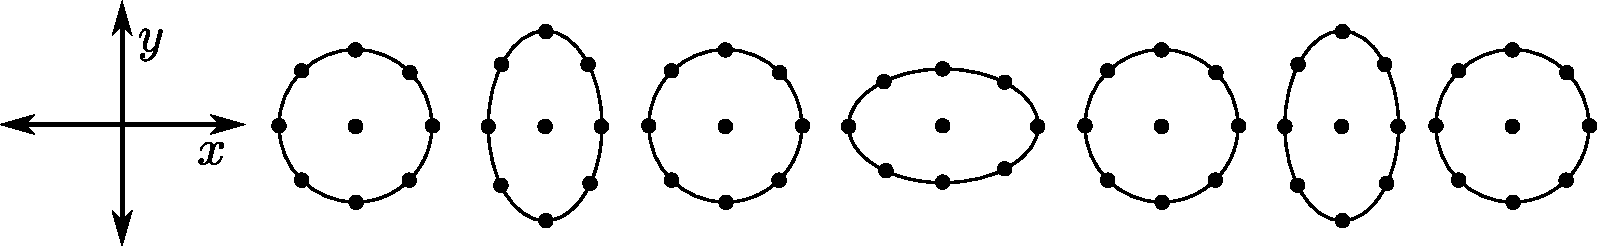
\psfig{file=fig/fig-onda-grav-mas.pdf,height=2.1cm,angle=0}}
\centerline{\psfig{file=fig/fig-onda-grav-cruz.pdf,height=2.1cm,angle=0}}
\centerline{\psfig{file=fig/fig-onda-grav-circular.pdf,height=2.1cm,angle=0}}
\caption{Oscilaciones inducidas por una onda gravitacional con polarizaci'on $+$, $\times$ y circular. Figuras adaptadas a partir de originales en \cite{Carroll97}.}
\label{fig:og}
\end{figure}
\end{center}
%\begin{center}
%\begin{figure}[H]
%\centerline{\psfig{file=fig-onda-grav-cruz.pdf,height=2.3cm,angle=0}}
%\caption{Oscilaciones inducidas por una onda gravitacional con polarizaci'on $\times$. Figura adaptada a partir de la original contenida en \cite{Carroll97}.}
%\label{fig:ogcruz}
%\end{figure}
%\end{center}
%\begin{center}
%\begin{figure}[H]
%\centerline{\psfig{file=fig-onda-grav-circular.pdf,height=2.3cm,angle=0}}
%\caption{Oscilaciones inducidas por una onda gravitacional con polarizaci'on circular. Figura adaptada a partir de la original contenida en \cite{Carroll97}.}
%\label{fig:ogccirc}
%\end{figure}
%\end{center}
Note que la amplitud del cambio de la distancia $L(\varphi)$ es $\delta L=Rh_+/2$, es decir,
\begin{equation}
\boxed{ \frac{\delta L}{L_0}\simeq h .}
\end{equation}
Se espera que los detectores de ondas gravitacionales interferom'etricos actuales alcancen una sensibilidad que permita detectar amplitudes hasta de $h\sim 10^{-20}$, que es tambi'en el orden de magnitud de la amplitud \textit{m'axima} de la radiaci'on gravitacional esperada en la Tierra debido a diversas fuentes astron'omicas. Por ejemplo, el proyecto \href{http://www.ligo.caltech.edu/}{LIGO}. consta de un interfer'ometro de 4\,km, de modo que deber'ia detectar fluctuaciones de distancia ($\delta L$) del orden de $10^{-17}\text{m}$, es decir, m'as peque\~nas que un n'ucleo at'omico!.

\begin{center}
\begin{figure}[H]
\centerline{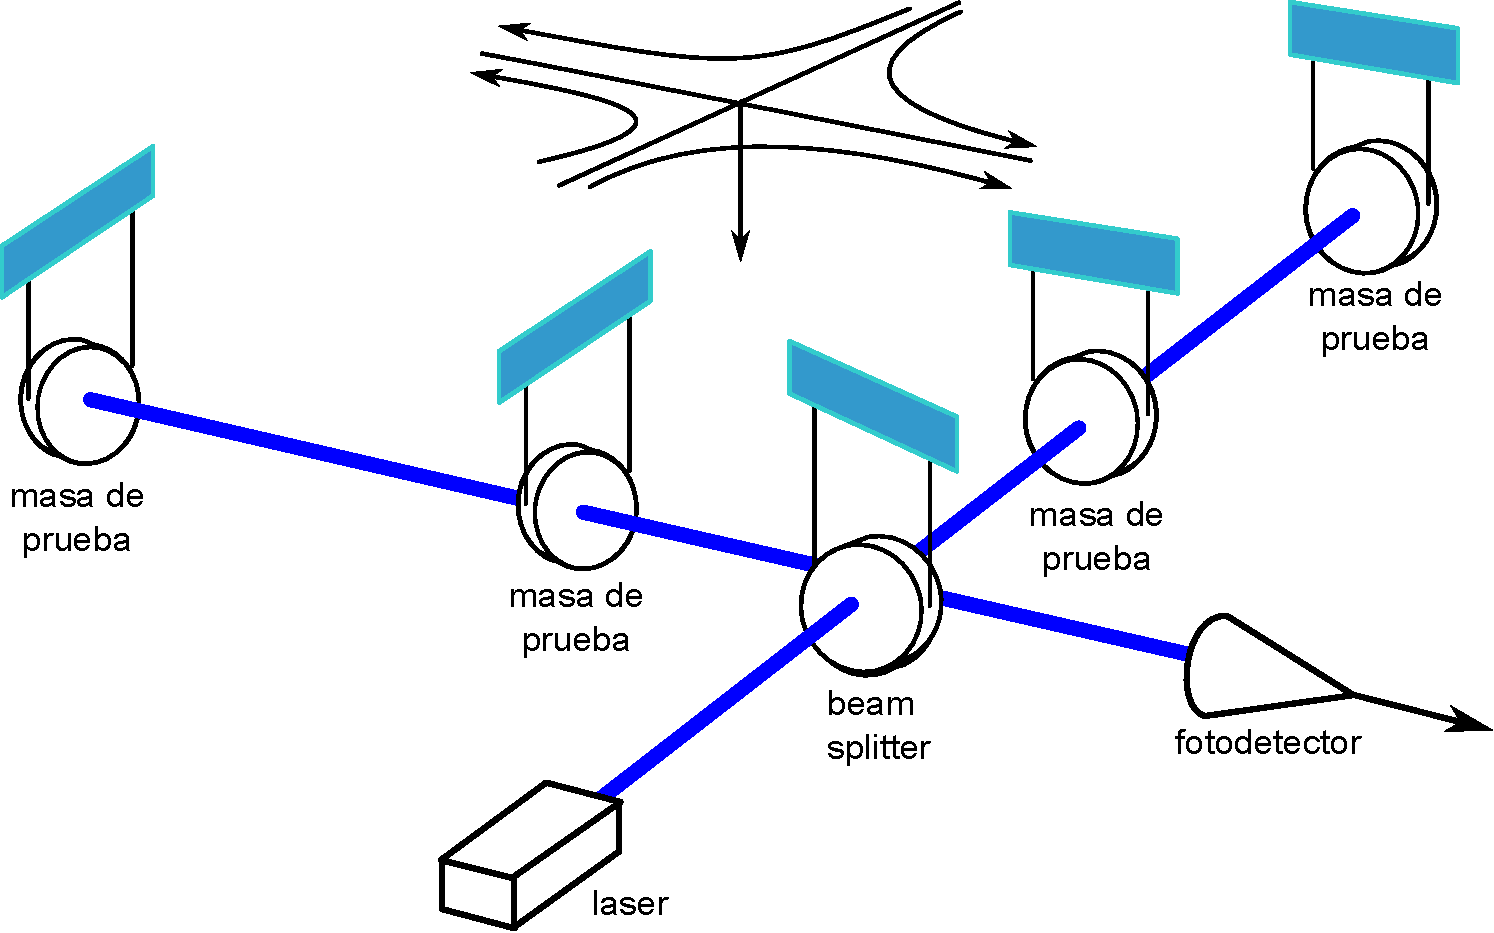
\psfig{file=fig/fig-LIGO.pdf,height=5cm,angle=0}}
\caption{Esquema de un detector interferom'etrico de ondas gravitacionales. Figura original \href{http://commons.wikimedia.org/wiki/File:Ligo.svg}{aqu'i}.}
\label{fig:LIGO}
\end{figure}
\end{center}
\section{Generaci'on de ondas gravitacionales}\label{sec:GOG}
Tal como en el caso de ondas electromagn'eticas, a distancias muy grandes (en la zona lejana o zona de radiaci'on, $r\gg\lambda$) y para fuentes peque\~nas (de tama\~no $L\ll\lambda$), encontramos que el t'ermino dominante de (\ref{solh}) es
\begin{equation}\label{hradT}
\bar{h}_{\rm rad}^{\mu\nu}(\vec{x},t)=-\frac{4G}{c^4} \frac{1}{r}\int T^{\mu\nu}_{(0)}(\vec{x}',t-\frac{r}{c})\, d^3x'.
\end{equation}
Adem'as, en una regi'on limitada del espacio, la onda puede aproximarse por una onda plana. En el gauge de Lorenz, toda la informaci'on de la onda est'a contenida en las componentes puramente espaciales $\bar{h}^{ij}$, ver (\ref{AA}). Adem'as, podemos expresar la integral (retardada) $\int T^{ij}_{(0)}\,d^3x$ en t'erminos de derivadas del momento cuadrupolar de la fuente. En efecto, usando la ley de conservaci'on para el tensor de energ'ia-momentum $T^{\mu\nu}_{(0)}$, podemos escribir
\begin{eqnarray}
 \int \partial_k(T^{ik}_{(0)}x^j)\,d^3x&=&\int (\partial_kT^{ik}_{(0)})x^j\,d^3x +\int T^{ij}_{(0)}\,d^3x \\
&=&-\int (\partial_0T^{i0}_{(0)})x^j\,d^3x +\int T^{ij}_{(0)}\,d^3x \\
&=&-\frac{1}{c}\frac{d\ }{dt}\int T^{i0}_{(0)}x^j\,d^3x +\int T^{ij}_{(0)}\,d^3x .
\end{eqnarray}
Pero la expresi'on del lado izquierdo puede transformarse en una integral de superficie en la frontera del volumen de integraci'on, que encierra la distribuci'on de energ'ia-momentum que genera el campo gravitacional. Asumiendo que esta distribuci'on est'a confinada a una regi'on acotada del espacio, tendremos que la integral de superficie se anula y por lo tanto
\begin{equation}
 \int T^{ij}_{(0)}\,d^3x =\frac{1}{c}\frac{d\ }{dt}\int T^{i0}_{(0)}x^j\,d^3x.
\end{equation}
Ya que $T^{ij}$ es sim'etrico podemos equivalentemente escribir
\begin{equation}\label{intT1}
 \int T^{ij}_{(0)}\,d^3x =\frac{1}{2c}\frac{d\ }{dt}\int \left(T^{i0}_{(0)}x^j+T^{j0}_{(0)}x^i\right)\,d^3x.
\end{equation}
Efectuamos ahora un an'alisis similar con la expresi'on $\int\partial_k(T^{0k}_{(0)}x^ix^j)\,d^3x$, que tambi'en es nula debido a que puede transformarse a una integral de superficie fuera de la regi'on con fuentes:
\begin{eqnarray}
 0&=&\int\partial_k(T^{0k}_{(0)}x^ix^j)\,d^3x\\
&=&\int(\partial_kT^{0k}_{(0)})x^ix^j\,d^3x+\int \left(T^{0i}_{(0)}x^j+T^{0j}_{(0)}x^i\right)\,d^3x\\
&=&-\int(\partial_0T^{00}_{(0)})x^ix^j\,d^3x+\int \left(T^{0i}_{(0)}x^j+T^{0j}_{(0)}x^i\right)\,d^3x\\
&=&-\frac{1}{c}\frac{d\ }{dt}\int T^{00}_{(0)}x^ix^j\,d^3x+\int \left(T^{0i}_{(0)}x^j+T^{0j}_{(0)}x^i\right)\,d^3x.
\end{eqnarray}
Por lo tanto,
\begin{equation}\label{intT2}
 \int \left(T^{0i}_{(0)}x^j+T^{0j}_{(0)}x^i\right)\,d^3x=\frac{1}{c}\frac{d\ }{dt}\int T^{00}_{(0)}x^ix^j\,d^3x.
\end{equation}
De esta forma, usando (\ref{intT1}) y (\ref{intT2}) encontramos que
\begin{equation}
 \int T^{ij}_{(0)}\,d^3x=\frac{1}{2c^2}\frac{d^2\ }{dt^2}\int T^{00}_{(0)}x^ix^j\,d^3x,
\end{equation}
y entonces
\begin{equation}
\bar{h}_{\rm rad}^{ij}(\vec{x},t)=-\frac{2G}{c^4} \frac{1}{r}\frac{d^2\ }{dt^2}\left[\frac{1}{c^2}\int T^{00}_{(0)}(x')\,x'^ix'^j\,d^3x'\right]_{\rm ret}.
\end{equation}
Como $T^{00}_{(0)}/c^2=\rho(\vec{x},t)$ es la densidad de masa de la fuente (a primer orden), se acostumbra escribir
\begin{equation}\label{hrad}
\boxed{\bar{h}_{\rm rad}^{ij}(\vec{x},t)=-\frac{2G}{c^4} \frac{1}{r}\left[\ddot{M}^{ij}\right]_{\rm ret},}
\end{equation}
donde
\begin{equation}
M^{ij}(t):=\int \rho(\vec{x},t)\,x^ix^j\,d^3x,
\end{equation}
es el \textit{tensor momento de inercia} (con traza) de la fuente.

Note que $\bar{h}_{\rm rad}^{ij}$ (b'asicamente, el potencial gravitacional de la onda generada) decae con $1/r$ y que la primera contribuci'on no nula corresponde a \textit{radiaci'on cuadrupolar}. Esta diferencia con el caso de ondas electromagn'eticas se debe a que la derivada temporal del \textit{momento dipolar gravitacional} $\int \rho x^i\,d^3x$ es proporcional al momentum lineal del sistema, que es conservado (constante) a primer orden, por lo que no aporta a la energ'ia radiada (que depende de la derivada de $\bar{h}_{\rm rad}^{ij}$).

\subsection{Ejemplo}
Consideremos un ejemplo sencillo, en el que dos cuerpos, cada uno de masa $M$, con una separaci'on $2R$, rotan con velocidad angular $\omega$ en un movimiento no-relativista en torno al centro de masa del sistema. Si modelamos las posiciones de ambas masas por $\vec{x}=\pm(R\cos(\omega t),R\sen(\omega t),0)$, es decir en el plano $xy$ y con posiciones iniciales en el eje $x$, tendremos que (la segunda derivada d)el tensor momento de inercia ser'a
\begin{equation}
 \ddot{M}^{ij}=-4MR^2\omega^2\left(
\begin{array}{ccc}
 \cos(2\omega t) & \sen(2\omega t) &0 \\
\sen(2\omega t) & -\cos(2\omega t) &0 \\
0&0&0
\end{array}\right).
\end{equation}
Con esto, (\ref{hrad}) implica que
\begin{eqnarray}
\bar{h}_{\rm rad}^{ij}(\vec{x},t)&=&\frac{8GMR^2\omega^2}{c^4r}\left(
\begin{array}{ccc}
 \cos\left[2\omega(t-r/c)\right] & \sen\left[2\omega(t-r/c)\right] &0\\
\sen\left[2\omega(t-r/c)\right] & -\cos\left[2\omega(t-r/c)\right] &0\\
0&0&0
\end{array}\right)\\
&=&\frac{8GMR^2\omega^2}{c^4r}\left[
\left(\begin{array}{ccc} 1 & 0 & 0\\ 0 & -1 &0 \\ 0&0&0\end{array}\right) \cos\left[2\omega(t-r/c)\right]
+\left(\begin{array}{ccc} 0 & 1 &0 \\ 1 & 0&0\\ 0&0&0\end{array}\right) \sen\left[2\omega(t-r/c)\right]
\right] \nonumber\\
&=&\frac{8GMR^2\omega^2}{c^4r}\Re\left[
\left(\begin{array}{ccc} 1 & 0 &0 \\ 0 & -1 &0 \\ 0&0&0\end{array}\right) e^{i\left[2\omega(t-\frac{r}{c})\right]} +\left(\begin{array}{ccc} 0 & 1 &0 \\ 1 & 0 &0 \\ 0&0&0\end{array}\right) e^{i\left[2\omega(t-\frac{r}{c})-\frac{\pi}{2}\right]}
\right] .
\end{eqnarray}
Vemos de aqu'i que \textit{un observador ubicado en un punto sobre el eje} $z$ detectar'a una onda gravitacional de frecuencia angular $2\omega$, que \textit{satisface autom'aticamente el gauge TT}, y que es una combinaci'on lineal de las polarizaciones $+$ y $\times$, con una diferencia de fase de $\pi/2$. Este estado es an'alogo al de una onda electromagn'etica con polarizaci'on circular.

El orden de magnitud de la amplitud de la onda es dada por
\begin{equation}
 h\simeq\frac{8GMR^2\omega^2}{c^4r}=8\left( \frac{GM}{c^2}\right) \left( \frac{1}{r}\right) \left( \frac{\omega R}{c}\right)^2 =8\left( \frac{m}{r}\right) \left( \frac{v}{c}\right) ^2.
\end{equation}
Por ejemplo, el pulsar binario PSR 1913+16 consta de 2 estrellas de neutrones de masa $M\approx 1.4 M_\odot$, con periodo orbital $T\approx 8\text{\,h}\approx 3\times 10^4\text{\,s}$, velocidades orbitales $v\simeq 10^2\text{\,km/s}$, a una distancia $r\approx 2\times 10^4\text{\, ly}\approx 10^{20}\text{\, m}$. En este caso, $m\approx 2\text{\,km}$, $v/c\simeq 3\times 10^{-4}$ y entonces $h\simeq 10^{-23}$ para la radiaci'on recibida en la Tierra, a una frecuencia del orden de $10^{-4}Hz$ (no detectable con LIGO).





 \section{Expansi'on hasta orden cuadr'atico en \texorpdfstring{$G$}{G}}
\subsubsection{M'etrica}

Ahora obtendremos una expresi'on para las ecuaciones de Einstein a segundo orden, es decir, aquellas que son cuadr'aticas en la constante gravitacional. Naturalmente, esta ecuaci'on de segundo orden en nuestro esquema perturbativo depender'a linealmente de la perturbaci'on de segundo orden de la m'etrica $h^{(2)}_{\mu\nu}$ y cuadr'aticamente de la perturbaci'on de primer orden $h^{(1)}_{\mu\nu}$.

Calculamos primero la perturbaci'on de orden 2 de la m'etrica inversa, que resulta ser 
\begin{equation}
g^{\mu\nu}_{(2)}=-h^{\mu\nu}_{(2)}+ h^{\mu\lambda}_{(1)}h_{(1)}{}_\lambda^{\ \nu} ,
\end{equation}
y donde hemos usado una notaci'on similar a la usada para las perturbaciones de primer orden para simbolizar las contracciones con la m'etrica plana $\eta$.

\subsubsection{Conexi'on}
Similarmente, la perturbaci'on de orden 2 de la conexi'on tiene la forma
\begin{equation}
\Gamma^\lambda_{(2)\mu\nu}=\frac{1}{2}\left(\partial_\mu h^\lambda_{(2)\nu} + \partial_\nu h^\lambda_{(2)\mu} -\partial^\lambda h^{(2)}_{\mu\nu}\right)
-\frac{1}{2}h_{(1)}^{\lambda\rho}\left(\partial_\mu
h^{(1)}_{\nu\rho} +\partial_\nu h^{(1)}_{\mu\rho} - \partial_\rho h^{(1)}_{\mu\nu}\right).
\end{equation}

\subsubsection{Tensor de Ricci}
Por otro lado, la componente cuadr'atica en $G$ del tensor de Ricci puede escribirse como
\begin{align}
R^{(2)}_{\mu\lambda} = &\ \frac{1}{2}\left(\partial_\mu\partial_\nu h^\nu_{(2)\lambda}+ \partial_\lambda \partial^\nu h^{(2)}_{\mu\nu} - \partial_\mu\partial_\lambda h^{(2)} -\square h^{(2)}_{\mu\lambda}\right) \\
& +\frac{1}{2}\left[\frac{1}{2}(\partial_\lambda h^{\sigma\rho}_{(1)})(\partial_\mu h_{\sigma\rho}^{(1)})+h^{\sigma\rho}_{(1)}\left(\partial_\lambda\partial_\mu h^{(1)}_{\sigma\rho}-\partial_\rho\partial_\mu h^{(1)}_{\lambda\sigma}-\partial_\rho\partial_\lambda h^{(1)}_{\mu\sigma}+ \partial_\rho\partial_\sigma h^{(1)}_{\mu\lambda}\right) \right.\\
& \left.+ (\partial_\sigma h^\rho_{(1)\lambda})\left(\partial^\sigma h^{(1)}_{\mu\rho}-\partial_\rho h^\sigma_{(1)\mu}\right) -\partial_\rho\left(h^{\sigma\rho}_{(1)}-\frac{1}{2}\eta^{\sigma\rho}\,h^{(1)}\right)\left(\partial_\mu h^{(1)}_{\lambda\sigma}+\partial_\lambda h^{(1)}_{\mu\sigma}-\partial_\sigma h^{(1)}_{\mu\lambda}\right) \right]\\
=&\ \frac{1}{2}\left(\partial_\mu\partial_\nu h^\nu_{(2)\lambda}+ \partial_\lambda \partial^\nu h^{(2)}_{\mu\nu} - \partial_\mu\partial_\lambda h^{(2)} -\square h^{(2)}_{\mu\lambda}\right) +A_{\mu\lambda},
\end{align}
donde hemos definido
\begin{align}
A_{\mu\lambda} := & \ \frac{1}{2}\left[\frac{1}{2}(\partial_\lambda h^{\sigma\rho}_{(1)})
(\partial_\mu h_{\sigma\rho}^{(1)})+h^{\sigma\rho}_{(1)}
\left(\partial_\lambda\partial_\mu h^{(1)}_{\sigma\rho}-\partial_\rho\partial_\mu
h^{(1)}_{\lambda\sigma}-\partial_\rho\partial_\lambda h^{(1)}_{\mu\sigma}
+ \partial_\rho\partial_\sigma h^{(1)}_{\mu\lambda}\right) \right. \nonumber\\
& + \left.  (\partial_\sigma h^\rho_{(1)\lambda})\left(\partial^\sigma h^{(1)}_{\mu\rho}-\partial_\rho h^\sigma_{(1)\mu}\right) -\partial_\rho\left(h^{\sigma\rho}_{(1)}-\frac{1}{2}\eta^{\sigma\rho}\,h^{(1)}\right)\left(\partial_\mu h^{(1)}_{\lambda\sigma}+\partial_\lambda h^{(1)}_{\mu\sigma}-\partial_\sigma h^{(1)}_{\mu\lambda}\right) \right]. \label{defAmn}
\end{align}

\subsubsection{Escalar de Curvatura}
La correspondiente componente del escalar de curvatura resulta ser
\begin{align}
R^{(2)} = &\ \eta^{\mu\nu}R^{(2)}_{\mu\nu}-h_{(1)}^{\mu\nu}R^{(1)}_{\mu\nu} \\
= &\ \partial^\mu\partial^\nu h^{(2)}_{\mu\nu} - \square h^{(2)}
-\frac{1}{2}h_{(1)}^{\mu\lambda}\left(2\partial_\mu\partial_\nu h^\nu_{(1)\lambda}
- \partial_\mu\partial_\lambda h^{(1)} -\square h^{(1)}_{\mu\lambda}\right)
+ \eta^{\mu\nu}A_{\mu\nu} \\
= &\ \partial^\mu\partial^\nu h^{(2)}_{\mu\nu} - \square h^{(2)}
+h_{(1)}^{\sigma\rho}\left(\square h^{(1)}_{\sigma\rho}
-2\partial_\rho\partial_\nu \bar{h}^\nu_{(1)\sigma}\right)
+\frac{3}{4}(\partial^\mu h_{(1)}^{\sigma\rho})(\partial_\mu h^{(1)}_{\sigma\rho}) \\
& -\frac{1}{2}(\partial^\sigma h_{(1)}^{\rho\mu})(\partial_\rho h^{(1)}_{\sigma\mu})
-(\partial_\rho h_{(1)}^{\sigma\rho})(\partial_\mu \bar{h}^\mu_{(1)\sigma})
+\frac{1}{2}(\partial^\nu h^{(1)})(\partial_\mu \bar{h}^\mu_{(1)\nu})\\
= &\ \partial^\mu\partial^\nu h^{(2)}_{\mu\nu} - \square h^{(2)}
+B,
\end{align}
con
\begin{align}
B := &\ h_{(1)}^{\sigma\rho}\left(\square h^{(1)}_{\sigma\rho}
-2\partial_\rho\partial_\nu \bar{h}^\nu_{(1)\sigma}\right)
+\frac{3}{4}(\partial^\mu h_{(1)}^{\sigma\rho})(\partial_\mu h^{(1)}_{\sigma\rho}) -\frac{1}{2}(\partial^\sigma h_{(1)}^{\rho\mu})(\partial_\rho h^{(1)}_{\sigma\mu}) \nonumber \\
& -(\partial_\rho h_{(1)}^{\sigma\rho})(\partial_\mu \bar{h}^\mu_{(1)\sigma})
+\frac{1}{2}(\partial^\nu h^{(1)})(\partial_\mu \bar{h}^\mu_{(1)\nu})
. \label{defB}
\end{align}

\subsubsection{Tensor de Einstein}
Finalmente, la contribuci'on cuadratica en $G$ al tensor de Einstein es dada por
\begin{align}
G^{(2)}_{\mu\nu} & =  R^{(2)}_{\mu\nu}-\frac{1}{2}\eta_{\mu\nu}R^{(2)}-\frac{1}{2}h^{(1)}_{\mu\nu}R^{(1)}\\
& =  \frac{1}{2}\left[\partial_\mu\partial^\lambda h^{(2)}_{\lambda\nu}
+\partial_\nu\partial^\lambda h^{(2)}_{\lambda\mu} -
\partial_\mu\partial_\nu h^{(2)} -\square h^{(2)}_{\mu\nu}
-\eta_{\mu\nu}\left(\partial^\lambda \partial^\rho h^{(2)}_{\lambda\rho}
- \square h^{(2)}\right) \right]+C_{\mu\nu},
\end{align}
con
\begin{align}
C_{\mu\lambda} :=&\  A_{\mu\lambda}-\frac{1}{2}\,\eta_{\mu\lambda}\, B-\frac{1}{2}h^{(1)}_{\mu\lambda}R^{(1)}.
\end{align}
En t'erminos de $\bar{h}^{(2)}_{\mu\nu}$, tenemos
\begin{align}
G^{(2)}_{\mu\nu} = & -\frac{1}{2}\left[\square \bar{h}^{(2)}_{\mu\nu}
+\eta_{\mu\nu}\, \partial^\lambda\partial^\rho\bar{h}^{(2)}_{\lambda\rho}-
\partial_\mu\partial^\lambda\bar{h}^{(2)}_{\lambda\nu}
- \partial_\nu\partial^\lambda \bar{h}^{(2)}_{\lambda\mu}\right]
+C_{\mu\nu}.
\end{align}

Note que las todas las expresiones para las perturbaciones de segundo orden dependen de la perturbaci'on $h^{(2)}_{\mu\nu}$ exactamente de la misma forma que las expresiones de primer orden dependen de $h^{(1)}_{\mu\nu}$. Esto es consecuencia de la expansi'on de estamos realizando (en torno a la m'etrica plana, de orden 0), y de la consistencia de la separaci'on realizada de las ecuaciones de Einstein en t'erminos que dependen de distintas potencias de $G$. Como vemos, lo que diferencia las expresiones de segundo orden es que adem'as poseen t'erminos, necesariamente sumados a los primeros, que dependen cuadr'aticamente de (las derivadas de) $h^{(1)}_{\mu\nu}$.


\section{Ecuaciones de Einstein a segundo orden}
De esta forma, las ecuaciones de Einstein de segundo orden son
\begin{equation}\label{lee2g2}
\square \bar{h}^{(2)}_{\mu\nu}
+\eta_{\mu\nu}\, \partial^\lambda\partial^\rho\bar{h}^{(2)}_{\lambda\rho}-
\partial_\mu\partial^\lambda\bar{h}^{(2)}_{\lambda\nu}
- \partial_\nu\partial^\lambda \bar{h}^{(2)}_{\lambda\mu} -2C_{\mu\nu}=
-\frac{16\pi G}{c^4}T_{\mu\nu}^{(1)} \, ,
\end{equation}
o, llevando el t'ermino $C_{\mu\nu}$ al lado derecho,
\begin{equation}\label{lee2g3}
\boxed{\square \bar{h}^{(2)}_{\mu\nu}
+\eta_{\mu\nu}\, \partial^\lambda\partial^\rho\bar{h}^{(2)}_{\lambda\rho}-
\partial_\mu\partial^\lambda\bar{h}^{(2)}_{\lambda\nu}
- \partial_\nu\partial^\lambda \bar{h}^{(2)}_{\lambda\mu} =
-\frac{16\pi G}{c^4}\left(T_{\mu\nu}^{(1)}+t_{\mu\nu} \right)\, .}
\end{equation}
Aqu'i hemos introducido
\begin{equation}
t_{\mu\nu}:=-\frac{c^4}{8\pi G}\,C_{\mu\nu}, \label{deft}
\end{equation}
que se suma a la contribuci'on de primer orden del tensor de energ'ia-mom'entum de la materia. El lado derecho de (\ref{lee2g3}) depende de la distribuci'on de materia (que se supone conocida) y de $h^{(1)}_{\mu\nu}$. De esta forma, (\ref{lee2g3}) suministra una ecuaci'on para la perturbaci'on de segundo orden $h^{(2)}_{\mu\nu}$, que tiene la misma forma que aquella para la perturbaci'on de primer orden, ec. (\ref{lee}), pero con un ``t'ermino fuente'' dependiente de la distribuci'on de materia y de la perturbaci'on de primer orden de la m'etrica. Adem'as, tal como en el caso de primer orden, la cuadridivergencia del lado izquierdo de (\ref{lee2g3}) es id'enticamente nula por lo que, como consecuencia,
\begin{equation}
\partial_\nu\left(T^{\mu\nu}_{(1)}+t^{\mu\nu} \right)=0. \label{cTt}
\end{equation}
En otras palabras, y esta vez a diferencia de lo encontrado a primer orden, la correspondiente componente del tensor de energ'ia-mom'entum de la materia \textit{no es conservado por separado}, sino s'olo su suma con el (pseudo-)tensor (\ref{deft}). Puesto que $t^{\mu\nu}$ depende (cuadr'aticamente) de $h^{(1)}_{\mu\nu}$, es posible interpretarlo como un \textbf{tensor de energ'ia-mom'entum efectivo para campo gravitacional}. Entonces (\ref{cTt}) representa la conservaci'on, correcta hasta el orden lineal en $G$, de la energ'ia y el mom'entum total del sistema materia + campo gravitacional. Equivalentemente, sumando (\ref{cTt}) y (\ref{cT0}) podemos escribir
\begin{equation}
\boxed{\partial_\nu\left(T^{\mu\nu}_{(0,1)}+t^{\mu\nu} \right)=0,} \label{cT01t}
\end{equation}
donde $T^{\mu\nu}_{(0,1)}:=T^{\mu\nu}_{(0)}+T^{\mu\nu}_{(1)}$ es el tensor de energ'ia-mom'entum de las fuentes, correcto hasta orden lineal en $G$.

\subsection{Gauges}
A segundo orden,
\begin{align}\label{pc2}
h'^{(2)}_{\mu\nu} = &\ h^{(2)}_{\mu\nu}- \partial_\mu\xi_\nu^{(2)} - \partial_\nu\xi_\mu^{(2)}\\
&  -(\partial_\nu\xi^\rho_{(1)})h^{(1)}_{\mu\rho} -(\partial_\mu\xi^\lambda_{(1)})h^{(1)}_{\nu\lambda} \\
& +(\partial_\nu\xi^\lambda_{(1)})(\partial_\lambda\xi_\mu^{(1)})
+(\partial_\mu\xi^\lambda_{(1)})(\partial_\lambda\xi_\nu^{(1)})
+(\partial_\mu\xi^\lambda_{(1)})(\partial_\nu\xi_\lambda^{(1)}).
\end{align}
Podemos considerar las transformaciones generadas por $\xi^\mu_{(1)}$ y $\xi^\mu_{(2)}$ \textit{en forma secuencial}. Es decir, podemos efectuar \textit{primero} todas las transformaciones de gauge generadas por $\xi^\mu_{(1)}$ (y $\xi^\mu_{(2)}=0$) que sean necesarias para, por ejemplo, imponer las condiciones del gauge $TT$ a $h^{(1)}_{\mu\nu}$,  tendremos un tensor ``intermedio" $h^{\rm i, (2)}_{\mu\nu}$. A partir de este tensor intermedio, podemos \textit{posteriormente} realizar transformaciones de gauge generada por $\xi^\mu_{(2)}$ (y $\xi^\mu_{(1)}=0$). A partir de \eqref{pc2} vemos que estas transformaciones cambian $h^{(2)}_{\mu\nu}$ de forma similar a la transformaci'on de primer orden, ver (\ref{pc}):
\begin{align}\label{pc2b}
h'^{(2)}_{\mu\nu} = &\ h^{\rm i,(2)}_{\mu\nu}- \partial_\mu\xi_\nu^{(2)} - \partial_\nu\xi_\mu^{(2)}.
\end{align}
Por lo tanto, es posible elegir $\xi^\mu_{(2)}$ de modo que la perturbaci'on de segundo orden tambi'en satisfaga el gauge de Lorenz,
\begin{equation} \label{lgauge2}
\partial^\nu\bar{h}^{(2)}_{\mu\nu}\stackrel{!}{=} 0 \, .
\end{equation}

\subsection{Tensor de energ'ia-mom'entum del campo gravitacional: con gauges, en el vac'io}
De lo discutido en la secci'on \ref{sec:GL} sabemos que podemos elegir coordenadas de modo que $h^{(1)}_{\mu\nu}$ satisfaga el gauge de Lorenz, ec. (\ref{lgauge}). Bajo estas condiciones (\ref{defAmn}) se reduce a
\begin{align}
A_{\mu\lambda} := & \ \frac{1}{4}(\partial_\lambda h^{\sigma\rho}_{(1)})
(\partial_\mu h_{\sigma\rho}^{(1)})+\frac{1}{2}h^{\sigma\rho}_{(1)}
\left(\partial_\lambda\partial_\mu h^{(1)}_{\sigma\rho}-\partial_\rho\partial_\mu
h^{(1)}_{\lambda\sigma}-\partial_\rho\partial_\lambda h^{(1)}_{\mu\sigma}
+ \partial_\rho\partial_\sigma h^{(1)}_{\mu\lambda}\right) \\
& + \frac{1}{2} (\partial_\sigma h^\rho_{(1)\lambda})\left(\partial^\sigma h^{(1)}_{\mu\rho}-\partial_\rho h^\sigma_{(1)\mu}\right),
\end{align}
mientras que (\ref{defB}) implica que
\begin{equation}
B := %\ h_{(1)}^{\sigma\rho}\square h^{(1)}_{\sigma\rho} +
 \frac{3}{4}(\partial^\mu h_{(1)}^{\sigma\rho})(\partial_\mu h^{(1)}_{\sigma\rho}) -\frac{1}{2}(\partial^\sigma h_{(1)}^{\rho\mu})(\partial_\rho h^{(1)}_{\sigma\mu}) .
\end{equation}
Note que aqu'i fueron tambi'en usadas las ecuaciones de movimiento \textit{fuera de las fuentes}, es decir, $\square h^{(1)}_{\mu\nu}=0$
Adem'as, bajo las mismas condiciones, la contribuci'on de primer orden del escalar de curvatura, ec. (\ref{R1}), se anula, por lo que
\begin{align}
C_{\mu\lambda} =&\  A_{\mu\lambda}-\frac{1}{2}\,\eta_{\mu\lambda}\, B \\
 = & \  \frac{1}{4}(\partial_\lambda h^{\sigma\rho}_{(1)})
(\partial_\mu h_{\sigma\rho}^{(1)}) + \frac{1}{2} (\partial_\sigma h^\rho_{(1)\lambda})\left(\partial^\sigma h^{(1)}_{\mu\rho}-\partial_\rho h^\sigma_{(1)\mu}\right) \nonumber\\
& +\frac{1}{2}h^{\sigma\rho}_{(1)}
\left(\partial_\lambda\partial_\mu h^{(1)}_{\sigma\rho}-\partial_\rho\partial_\mu
h^{(1)}_{\lambda\sigma}-\partial_\rho\partial_\lambda h^{(1)}_{\mu\sigma}
+ \partial_\rho\partial_\sigma h^{(1)}_{\mu\lambda}\right)
\nonumber \\
& -\frac{1}{2}\,\eta_{\mu\lambda}\left[ \frac{3}{4}(\partial^\nu h_{(1)}^{\sigma\rho})(\partial_\nu h^{(1)}_{\sigma\rho})
-\frac{1}{2}(\partial^\sigma h_{(1)}^{\rho\nu})(\partial_\rho h^{(1)}_{\sigma\nu})\right] .
\end{align}

Para calcular la \textit{potencia radiada} necesitamos las componentes $C_{0i}$:
\begin{align}
C_{0i} = & \  \frac{1}{4}(\partial_i h^{\sigma\rho}_{(1)})(\partial_0 h_{\sigma\rho}^{(1)}) +\frac{1}{2} h^{\sigma\rho}_{(1)}\left(\partial_i\partial_0 h^{(1)}_{\sigma\rho}-\partial_\rho\partial_0
h^{(1)}_{i\sigma}-\partial_\rho\partial_i h^{(1)}_{0\sigma}
+ \partial_\rho\partial_\sigma h^{(1)}_{0i}\right) \nonumber \\
& + \frac{1}{2} (\partial_\sigma h^\rho_{(1)i})\left(\partial^\sigma h^{(1)}_{0\rho}-\partial_\rho h^\sigma_{(1)0}\right). \label{C0ia}
\end{align}

\subsubsection{Potencia Radiada: gauge de TT en zona de radiaci'on}
Sin dejar el gauge de Lorenz es posible adem'as imponer, fuera de las fuentes, el gauge TT, es decir, las condiciones  (\ref{ttg}), que a su vez implican las relaciones (\ref{dh00}). Usando estas expresiones, (\ref{C0ia}) se reduce a
\begin{align}
C_{0i} = & \  \frac{1}{4}(\partial_i h^{jk}_{(1)})(\partial_0 h_{jk}^{(1)})
+\frac{1}{2}h^{jk}_{(1)}\left(\partial_i\partial_0 h^{(1)}_{jk} -\partial_k\partial_0 h^{(1)}_{ij}\right) - \frac{1}{2}(\partial_0 h^j_{(1)i})(\partial_j h^0_{(1)0}).
\end{align}
Para conseguir una simplificaci'on adicional, consideramos que en la \textit{zona de radiaci'on} (l'imite de campo lejano) los campos (que representan ondas \textit{salientes}) satisfacen la relaci'on\footnote{Esta relaci'on puede tambi'en derivarse a partir de la forma asint'otica de la soluci'on de la ecuaci'on de onda en coordenadas esf'ericas.}, ver (\ref{hradT}),
\begin{equation}\label{zrad}
\partial_i h^{(1)}_{jk}=-\frac{\hat{r}_i}{c}\partial_t h^{(1)}_{jk}+O(r^{-2}),
\end{equation}
donde $\hat{r}_i=\hat{r}^i:=x^i/r$ es el vector unitario correspondiente al vector que une las fuentes con el punto de observaci'on.

Podemos entonces usar \eqref{zrad} para convertir todas las derivadas espaciales de $h^{(1)}_{ij}$ en t'erminos proporcionales a derivadas temporales:
\begin{align}
c^2C_{0i} = & -\frac{1}{4}(\hat{r}_i\partial_t h^{jk}_{(1)})(\partial_t h_{jk}^{(1)})
-\frac{1}{2}h^{jk}_{(1)}\left(\hat{r}_i\partial^2_t h^{(1)}_{jk}-\hat{r}_k\partial^2_t
h^{(1)}_{ij}\right)
+ \frac{1}{2}(\partial_t h^j_{(1)i})(\hat{r}_j \partial_t h^0_{(1)0})\\
= & -\frac{1}{4}(\hat{r}_i\partial_t h^{jk}_{(1)})(\partial_t h_{jk}^{(1)})
-\frac{1}{2}h^{jk}_{(1)}\left(\hat{r}_i\partial^2_t h^{(1)}_{jk}-\hat{r}_k\partial^2_t
h^{(1)}_{ij}\right) \\
= & -\frac{1}{4}\hat{r}_i\,\dot{h}_{jk}^{(1)}\dot{h}_{jk}^{(1)}
-\frac{1}{2}\partial_t\left(\hat{r}_i h^{jk}_{(1)}\dot{h}^{(1)}_{jk}-\hat{r}_kh^{jk}_{(1)}\dot{h}^{(1)}_{ij}\right)
+\frac{1}{2}\hat{r}_i\dot{h}^{(1)}_{jk}\dot{h}^{(1)}_{jk}
-\frac{1}{2}\hat{r}_k\,\dot{h}^{jk}_{(1)}\dot{h}^{(1)}_{ij}\\
= &\ \frac{1}{4}\,\hat{r}_i\,\dot{h}_{jk}^{(1)}\dot{h}_{jk}^{(1)} -\frac{1}{2}\partial_t\left(\hat{r}_i h^{jk}_{(1)}\dot{h}^{(1)}_{jk}-\hat{r}_kh^{jk}_{(1)}\dot{h}^{(1)}_{ij}\right)
-\frac{1}{2}\hat{r}_k\,\dot{h}^{jk}_{(1)}\dot{h}^{(1)}_{ij} \label{c2c0i}\\
= &\ \frac{1}{4}\,\hat{r}_i\,\dot{h}_{jk}^{(1)}\dot{h}_{jk}^{(1)}
-\frac{1}{2}\partial_t\left(\hat{r}_i h^{jk}_{(1)}\dot{h}^{(1)}_{jk} -\hat{r}_kh^{jk}_{(1)}\dot{h}^{(1)}_{ij}\right).
\end{align}
En el 'ultimo paso se us'o el hecho que (\ref{dh00}b) y (\ref{zrad}) implican que el 'ultimo t'ermino del lado derecho de (\ref{c2c0i}) se anula.

Finalmente, como es usual en procesos continuos de emisi'on de energ'ia, es 'util considerar el \textit{promedio temporal} de la potencia radiada. Este promedio es definido en general por
\begin{equation}
\left\langle f\right\rangle :=\frac{1}{T}\int_0^T f(t')\,dt'.
\end{equation}
Como consecuencia, el promedio de cualquier funci'on que es la \textit{derivada temporal de una funci'on acotada} (tal como la amplitud $h_{ij}^{(1)}$), en un intervalo de tiempo mucho mayor que el periodo t'ipico de variaci'on de la funci'on, tiende a cero, ya  que
\begin{equation}
\left\langle \frac{dg}{dt}\right\rangle=\frac{g(T)-g(0)}{T}\to 0.
\end{equation}
Usando esto, encontramos que
\begin{equation}
\left\langle c^2C_{0i}\right\rangle=\frac{1}{4}\,\hat{r}_i\left\langle\dot{h}_{jk}^{(1)}\dot{h}_{jk}^{(1)}\right\rangle .
\end{equation}

La potencia promedio radiada por las ondas gravitacionales es entonces dada por
\begin{align}
\left\langle P\right\rangle =& \oint r^2 \left\langle ct^{0i}\right\rangle\hat{r}_i\,d\Omega\\
=& \frac{c^5}{8\pi G}\oint r^2\left\langle C_{0i}\right\rangle\hat{r}_i\,d\Omega\\
=& \frac{c^3}{32\pi G} \oint r^2\left\langle\dot{h}_{jk}^{(1)}\dot{h}_{jk}^{(1)}\right\rangle\,d\Omega .
\end{align}

En otras palabras, la \textit{potencia promedio radiada por unidad de 'angulo s'olido} es
\begin{equation}\label{PTT}
\boxed{\left\langle\frac{d P}{d\Omega}\right\rangle=\frac{c^3r^2}{32\pi G} \left\langle\dot{h}_{ij}^{(1,\rm TT)}\dot{h}_{ij}^{(1,\rm TT)}\right\rangle .}
\end{equation}
En esta 'ultima expresi'on hemos agregado el signo $TT$ para indicar que este resultado es v'alido cuando el campo $h^{(1)}_{ij}$ est'a expresado en el gauge transversal sin traza, $h^{(1)}_{ij}=h^{(1,\rm TT)}_{ij}$.

\section{F'ormula cuadrupolar para la potencia radiada}
Tal como vimos en la secci'on \ref{sec:GOG}, en la zona de radiaci'on ($r\gg\lambda$) el campo $h^{(1)}_{\mu\nu}$ producido por una fuente peque\~na ($L\ll\lambda$) es dado por la expresi'on (\ref{hrad}). Sin embargo, (\ref{hrad}) es v'alido en coordenadas usadas tanto dentro como fuera de las fuentes, y en general no satisface las condiciones (adicionales a las del gauge de Lorenz) del gauge TT. Por esto, no es posible usar directamente (\ref{PTT}), para el campo dado por (\ref{hrad}). Es posible, sin embargo, \textit{transformar} el campo (\ref{hrad}) al gauge TT, por medio de una transformaci'on de gauge apropiada. Como primer paso para esta transformaci'on, generalizaremos el proceso aplicado en la secci'on \ref{sec:OGP}, al caso de una onda plana propag'andose en una direcci'on arbitraria, y luego al caso de una onda esf'erica en la zona de radiaci'on.

\subsection{Transformaci'on de una onda plana}\label{sec:TOP}
Tal como en la secci'on \ref{sec:OGP}, consideramos una onda plana de la forma (\ref{op}), con una ampitud $A_{\mu\nu}$ que satisface la condici'on de Lorenz  (\ref{glA}). Esto permite escribir
\begin{equation}
 (k^0)^2=-k_ik^i=:+\vec{k}^2.
\end{equation}
Esta vez, sin embargo, con un vector de onda $\vec{k}$ tiene una direcci'on arbitraria. La condici'on (\ref{glA}) permite expresar las componentes de $A_{00}$ y $A_{0i}$ en t'erminos de las componentes puramente espaciales de $A_{\mu\nu}$,
\begin{equation}\label{A000i}
A_{00}=A_{ij}n^in^j, \qquad A_{0i}=-A_{ij}n^j,
\end{equation}
donde hemos introducido el vector (tridimensional) unitario $n^i:=k^i/k^0$.

Realizamos ahora una transformaci'on de gauge de la forma (\ref{xiOP}), que induce la transformaci'on (\ref{AAp}) de la amplitud. Si imponemos la condiciones del gauge TT para el campo transformado, es decir, que $A'_{0i}=0$ y que $A':=A'^\mu_{ \mu}=0$, obtenemos las siguientes condiciones:
\begin{equation}
A_{0i}-\epsilon_0k_i-\epsilon_ik_0=0, \qquad
A+2\epsilon_0k^0+2\epsilon_ik^i=0.
\end{equation}
Estas cuatro condiciones permiten determinar 'unicamente las cuatro componentes del vector $\epsilon_\mu$, resultando:
\begin{align}
\epsilon_0 &= -\frac{1}{4k^0}\left(A+2A_{0i}n^i\right) ,\\
\epsilon_i &= \frac{1}{k^0}\left(A_{0i}+\frac{1}{4}An_i+\frac{1}{2}A_{0j}n_in^j\right).
\end{align}
Usando (\ref{A000i}) y $A=A_{00}+A^i_{\ i}$, podemos reescribir el resultado anterior como:
\begin{align}
\epsilon_0 &= \frac{1}{4k^0}\left(A_{ij}n^in^j-A^i_{\ i}\right) ,\\
\epsilon_i &= \frac{1}{k^0}\left(\frac{1}{4}A^j_{\ j}n_i-A_{ij}n^j-\frac{1}{4}A_{jk}n_in^jn^k\right).
\end{align}
Sustituyendo estos par'ametros en la transformaci'on de gauge de la amplitud (\ref{AAp}), obtenemos una expresi'on para las otras componentes de $A'_{\mu\nu}$:
\begin{equation}\label{AijTT}
A'_{ij} = A_{ij}+A_{jk}n_in^k+A_{ik}n_jn^k+\frac{1}{2}A_{kl}n_in_jn^kn^l-\frac{1}{2}A^k_{\ k}n_in_j+\frac{1}{2}A^k_{\ k}\delta_{ij}+\frac{1}{2}A_{kl}\delta_{ij}n^kn^l,
\end{equation}
mientras que
\begin{equation}
A'_{00} = 0.
\end{equation}
Finalmente, podemos escribir $A'_{ij}$ en (\ref{AijTT}) como la acci'on de un \textit{operador de proyecci'on} $\Lambda_{ij}^{\ \ kl}(\hat{n})$, definido por
\begin{equation}
\boxed{\Lambda_{ij}^{\ \ kl}(\hat{n}):=\delta^k_i\delta^l_j-\frac{1}{2}\delta_{ij}\delta^{kl}+\delta^l_jn_in^k+\delta^k_in_jn^l +\frac{1}{2}n_in_j\delta^{kl} +\frac{1}{2}\delta_{ij}n^kn^l
+\frac{1}{2}n_in_jn^kn^l,}
\end{equation}
de modo que
\begin{equation}
\boxed{A'_{ij}=\Lambda_{ij}^{\ \ kl}(\hat{n})\,A_{kl}.}
\end{equation}

Equivalentemente, y usando la convenci'on de escribir todas las componentes espaciales en forma contravariante, podemos escribir
\begin{equation}
A'^{ij}=\Lambda^{ij,kl}(\hat{n})\,A^{kl},
\end{equation}
con
\begin{equation}
\Lambda^{ij,kl}(\hat{n}):=\delta^{ik}\delta^{jl}-\frac{1}{2}\delta^{ij}\delta^{kl}-\delta^{jl}n^in^k-\delta^{ik}n^jn^l
+\frac{1}{2}n^in^j\delta^{kl} +\frac{1}{2}\delta^{ij}n^kn^l +\frac{1}{2}n^in^jn^kn^l .
\end{equation}
Es directo mostrar que este operador es completamente transversal a $n^i$, en el sentido que satisface
\begin{equation}
n^i\Lambda^{ij,kl}=n^j\Lambda^{ij,kl}=\Lambda^{ij,kl}n^k=\Lambda^{ij,kl}n^l\equiv 0.
\end{equation}
Adem'as, es libre de trazas, en el sentido que
\begin{equation}
\Lambda^{ii,kl}=\Lambda^{ij,kk}=0,
\end{equation}
Como consecuencia de estas propiedades, se satisface
\begin{equation}\label{LLL}
\Lambda^{ij,kl}\Lambda^{ij,pq}\equiv \Lambda^{kl,pq}.
\end{equation}
Finalmente, la siguiente identidad geom'etrica nos ser'a de utilidad
\begin{equation}\label{intL}
\oint\Lambda^{ij,kl}\,d\Omega=\frac{2\pi}{15}\left(11\delta^{ik}\delta^{jl}-4\delta^{ij}\delta^{kl}+\delta^{il}\delta^{jk}\right).
\end{equation}

\subsection{Transformaci'on de ondas esf'ericas en la zona de radiaci'on}\label{sec:TOER}

Es posible extender este resultado directamente al caso en que el campo original se escribe como una combinaci'on lineal de ondas planas. Sin embargo, en el caso particular en el que estamos interesados aqu'i, basta una discusi'on simplificada. Esto se debe a que, por un lado, para calcular la potencia promedio radiada s'olo los campos radiativos, que decaen con $1/r$ a grandes distancias, tienen una contribuci'on no nula. Adem'as, la expresi'on (\ref{hradT}) nos dice que
\begin{equation}\label{hradf}
\bar{h}_{\rm rad}^{\mu\nu}(\vec{x},t)= \frac{1}{r}\left.A^{\mu\nu}\right|_{t-r/c}, \qquad A^{\mu\nu}(t):=-\frac{4G}{c^4}\int T^{\mu\nu}_{(0)}(\vec{x}',t)\, d^3x'.
\end{equation}
Por lo tanto, la perturbaci'on de primer orden requerida depende de la distancia $r$ a las fuentes a trav'es del factor global $1/r$ y a trav'es de la dependencia temporal de $A^{\mu\nu}(t)$, ya que esta funci'on (de una variable) debe ser evaluada en el tiempo retardado $t_{\rm ret}=t-r/c$. En resumen, en el caso de presente inter'es el campo a considerar tiene una dependencia espacial simple, lo que reduce considerablemente los c'alculos.

Consideramos primero la descomposici'on de Fourier (temporal) de la funci'on $A^{\mu\nu}(t)$,
\begin{equation}\label{FIij}
A^{\mu\nu}(t)=\frac{1}{\sqrt{2\pi}}\int_{-\infty}^\infty \tilde{A}^{\mu\nu}(\omega)e^{i\omega t}\,d\omega,
\end{equation}
donde
\begin{equation}
\tilde{A}^{\mu\nu}(\omega)=\frac{1}{\sqrt{2\pi}}\int_{-\infty}^\infty A^{\mu\nu}(t)e^{-i\omega t}\,dt.
\end{equation}
Usando (\ref{FIij}) podemos escribir (\ref{hrad}) como
\begin{equation}\label{Fhrad}
\bar{h}_{\rm rad}^{\mu\nu}(\vec{x},t)=\frac{1}{\sqrt{2\pi}}\int_{-\infty}^\infty \tilde{A}^{\mu\nu}(\omega)\frac{e^{i\omega (t-r/c)}}{r}\,d\omega,
\end{equation}
es decir, como una superposici'on de ondas esf'ericas. Cada una de estas ondas puede escribirse como $e^{i\omega (t-r/c)}=e^{ik_\mu x^\mu}$, con $k^0=\omega/c$ y $k^i=(\omega/c)\,\hat{r}^i$, donde $\hat{r}^i$ es el vector radial unitario desde la fuente al punto de observaci'on (es decir, $\hat{r}^i=x^i/r$). Para transformar (\ref{Fhrad}) al gauge TT aplicamos la transformaci'on generada por (compare con (\ref{xiOP})):
\begin{equation}
\xi^\mu_{(1)}=\frac{1}{\sqrt{2\pi}}\int_{-\infty}^\infty (-i\epsilon^\mu)\frac{e^{ik_\mu x^\mu}}{r}\,d\omega, \qquad \epsilon^\mu=\epsilon^\mu(\omega,\hat{r}).
\end{equation}
Usando la ley general de transformaci'on (\ref{hp3}) y teniendo en cuenta la
dependencia de $\bar{h}_{\rm rad}^{\mu\nu}$ con $1/r$ es directo verificar que
el campo transformado contendr'a t'erminos que decaen con $1/r^2$, y por lo tanto no contribuyen al campo de radiaci'on. Por otro lado, los t'erminos radiativos (aquellos que decaen con $1/r$) ser'an de la forma
\begin{equation}
\bar{h}_{\rm rad}^{'\mu\nu}=\frac{1}{\sqrt{2\pi}}\int_{-\infty}^\infty \tilde{A}'^{\mu\nu}(\omega)\frac{e^{ik_\mu x^\mu}}{r}\,d\omega,
\end{equation}
con $\tilde{A}'^{\mu\nu}$ dado por la \textit{misma expresi'on} (\ref{AAp}) encontrada en el caso de ondas planas. Esto muestra que, para cada valor de $\omega$ y $\hat{n}=\hat{r}$ puede aplicarse el procedimiento descrito en \ref{sec:TOP}. Esto implica entonces que
\begin{align}
h_{{\rm rad}, TT}^{ij} &= \frac{1}{\sqrt{2\pi}}\int_{-\infty}^\infty \Lambda^{ij,kl}(\hat{r})\tilde{A}^{kl}(\omega)\frac{e^{ik_\mu x^\mu}}{r}\,d\omega \\
&= \frac{1}{\sqrt{2\pi}}\,\Lambda^{ij,kl}(\hat{r})\int_{-\infty}^\infty \tilde{A}^{kl}(\omega)\frac{e^{ik_\mu x^\mu}}{r}\,d\omega \\
&= \Lambda^{ij,kl}(\hat{r})\,\bar{h}_{\rm rad}^{kl},
\end{align}
mientras que $\bar{h}^{'\rm rad}_{0\mu}=0$. En resumen, la transformaci'on desde el campo de radiaci'on en el gauge de Lorenz hasta el gauge TT tiene la siguiente forma
\begin{equation}\label{hradTT}
\boxed{h_{{\rm rad}, TT}^{ij}(\vec{x},t)= \Lambda^{ij,kl}(\hat{r})\,\bar{h}_{\rm rad}^{kl}(t,r).}
\end{equation}
Introduciendo ahora la expresi'on (\ref{hradTT})  en  (\ref{PTT}) obtenemos
\begin{equation}\label{PGL}
\left\langle\frac{d P}{d\Omega}\right\rangle=\frac{c^3r^2}{32\pi G}\, \Lambda^{ij,kl}(\hat{r})\Lambda^{ij,pq}(\hat{r})\left\langle\dot{\bar{h}}_{\rm rad}^{kl}\dot{\bar{h}}_{\rm rad}^{pq}\right\rangle.
\end{equation}
Usando el resultado (\ref{LLL}) podemos escribir
\begin{equation}\label{PGL2}
\boxed{\left\langle\frac{d P}{d\Omega}\right\rangle=\frac{c^3r^2}{32\pi G}\, \Lambda^{ij,kl}(\hat{r})\left\langle\dot{\bar{h}}_{\rm rad}^{ij}\dot{\bar{h}}_{\rm rad}^{kl}
\right\rangle.}
\end{equation}
En virtud del resultado (\ref{hrad}), encontramos la siguiente expresi'on para la potencia promedio radiada por unidad de 'angulo s'olido:

\begin{equation}\label{PGL3}
\boxed{\left\langle\frac{d P}{d\Omega}\right\rangle=\frac{G}{8\pi c^5}\, \Lambda^{ij,kl}(\hat{r})\left\langle\dddot{M}^{ij}\dddot{M}^{kl}\right\rangle_{\rm ret} .}
\end{equation}
La identidad (\ref{intL}) permite encontrar una expresi'on simple para la potencia promedio total radiada. Al integrar, se encuentra que
\begin{equation}\label{intLII}
\oint\Lambda^{ij,kl}(\hat{r})\dddot{M}^{ij}
\dddot{M}^{kl}\,d\Omega=\frac{8\pi}{5}\left[\dddot{M}^{ij}\dddot{M}^{ij}-\frac{1}{3}(\dddot{M}^{ii})^2\right],
\end{equation}
obteniendo as'i que
\begin{equation}\label{PII}
\left\langle P\right\rangle =\frac{G}{5c^5}\, \left\langle \dddot{M}^{ij}\dddot{M}^{ij}-\frac{1}{3}\left(\dddot{M}^{ii}\right)^2\right\rangle_{\rm ret},
\end{equation}
o, en t'erminos del \textbf{momento cuadrupolar sin traza},
\begin{equation}\label{Qij}
Q^{ij}:=M^{ij}-\frac{1}{3}M^{kk}\delta^{ij},
\end{equation}
%\begin{equation}\label{intLII2}
%\oint\Lambda^{ij,kl}(\hat{r})\dddot{I}^{ij}
%\dddot{I}^{kl}\,d\Omega=\frac{8\pi}{5}\left(\dddot{Q}^{ij}\dddot{Q}^{ij}\right).
%\end{equation}
\begin{equation}\label{PTTQ}
\boxed{\left\langle P\right\rangle=\frac{G}{5c^5}\, \left\langle \dddot{Q}^{ij}\dddot{Q}^{ij}\right\rangle_{\rm ret} ,}
\end{equation}
que es la famosa f'ormula cuadrupolar para la potencia promedio total radiada.

In c'alculo algo m'as complicado \cite{Maggiore} permite adem'as determinar el \textit{momento angular promedio total transportado por las ondas gravitacionales, por unidad de tiempo}:
\begin{equation}\label{eqfinal}
\boxed{\left\langle\dot{L}^{i}\right\rangle=\frac{2G}{5c^{5}}\epsilon^{ijk} \left\langle\ddot{Q}^{jl}\dddot{Q}^{kl}\right\rangle_{\rm ret}.}
\end{equation}
\subsection{Ejemplo: Potencia radiada por un sistema binario}
Consideramos aqu'i el caso en que un sistema binario est'a conformado por masas compactas, que modelaremos como puntuales, orbitando una respecto a la otra por efecto de su atracci'on gravitacional mutua. Para esto, realizaremos los c'alculos (newtonianos) en el sistema de referencia del centro de masa, usando los resultados del ap'endice \ref{app:Kepler}.

Requerimos el tensor momento de inercia del sistema. Como es de esperar, puede mostrarse f'acilmente que el momento de inercia total del sistema binario se reduce al de una part'icula con masa reducida $\mu$, realizando un movimiento descrito por la coordenada relativa $\vec{r}$. Ver ap'endice \ref{app:Kepler} para los detalles:
\begin{equation}
M_{ij}=m_1x_i^{(1)}x_j^{(1)}+m_2x_i^{(2)}x_j^{(2)}=\mu\, r_i\,r_j.
\end{equation}
Si las coordenadas son elegidas de modo que el movimiento del sistema est'a confinado al plano $xy$, tendremos que s'olo $M_{11}$, $M_{12}$ y $M_{22}$ ser'an distintos de cero. De este modo, encontramos que
\begin{align}
M_{11} & = \mu\, x^2\\
& = \mu r^2\cos^2\varphi \\
& = \mu a^2(1-e^2)^2\frac{\cos^2\varphi}{\left[1+e\cos(\varphi-\varphi_0)\right]^2},
\end{align}
y, similarmente,
\begin{align}
M_{12} & = \mu\, xy \\
& = \mu r^2\cos\varphi\sen\varphi \\
& = \mu a^2(1-e^2)^2\frac{\sen\varphi\cos\varphi}{\left[1+e\cos(\varphi-\varphi_0)\right]^2},
\end{align}
\begin{align}
M_{22} & = \mu\, y^2 \\
& = \mu r^2\sen^2\varphi \\
& = \mu a^2(1-e^2)^2\frac{\sen^2\varphi}{\left[1+e\cos(\varphi-\varphi_0)\right]^2}.
\end{align}
A continuaci'on requerimos determinar las terceras derivadas $\dddot{I}_{ij}$. Para esto, introducimos la coordenada angular $\varphi$ y usamos (\ref{Ln}) y (\ref{rphi}), de modo que podamos escribir
\begin{align}
\dot{M}_{ij} &= \frac{dM_{ij}}{d\varphi}\dot{\varphi} \\
&= \frac{dM_{ij}}{d\varphi}\frac{L}{\mu r^2} \\
&= \frac{L}{\mu a^2(1-e^2)^2}\left[1+e\cos(\varphi-\varphi_0)\right]^2 \frac{dI_{ij}}{d\varphi}\\
&= \frac{\omega_0}{(1-e^2)^{3/2}}\left[1+e\cos(\varphi-\varphi_0)\right]^2 \frac{dI_{ij}}{d\varphi}.
\end{align}
Luego de algo de 'algebra encontramos que
\begin{equation}
\dot{M}_{11}=(-2)\mu a^2\omega_0\left(1-e^2\right)^{1/2}\frac{\cos\varphi(\sen\varphi+e\sen\varphi_0)}{1+e\cos(\varphi-\varphi_0)},
\end{equation}
\begin{equation}
\dot{M}_{22}=(+2)\mu a^2\omega_0\left(1-e^2\right)^{1/2}\frac{\sen\varphi(\cos\varphi+e\cos\varphi_0)}{1+e\cos(\varphi-\varphi_0)},
\end{equation}
\begin{equation}
\dot{M}_{12}=\mu a^2\omega_0\left(1-e^2\right)^{1/2}\frac{(\cos2\varphi+e\cos(\varphi+\varphi_0))}{1+e\cos(\varphi-\varphi_0)}.
\end{equation}

An'alogamente, encontramos que
\begin{equation}\label{I11}
\dddot{M}_{11}=\alpha\left[1+e\cos(\varphi-\varphi_0)\right]^2 \left[4\sen(2\varphi)+3e\sen(2\varphi)\cos(\varphi-\varphi_0)
+2e\cos\varphi\sen\varphi_0\right],
\end{equation}
\begin{equation}\label{I22}
\dddot{M}_{22}=\alpha\left[1+e\cos(\varphi-\varphi_0)\right]^2 \left[-4\sen(2\varphi)-3e\sen(2\varphi)\cos(\varphi-\varphi_0)
-2e\sen\varphi\cos\varphi_0\right],
\end{equation}
\begin{equation}\label{I12}
\dddot{M}_{12}=\alpha\left[1+e\cos(\varphi-\varphi_0)\right]^2 \left[-4\cos(2\varphi)-3e\cos(2\varphi)\cos(\varphi-\varphi_0)
-e\cos(\varphi+\varphi_0)\right],
\end{equation}
con
\begin{equation}
\alpha:=\frac{\mu a^2\omega_0^3}{\left(1-e^2\right)^{5/2}}.
\end{equation}
En t'erminos del tensor momento de inercia con traza, la potencia promedio radiada es dada por (\ref{PII}), y se reduce en este caso a
\begin{align}
\left\langle P\right\rangle &=\frac{G}{5c^5}\, \left\langle \dddot{M}^{ij}\dddot{M}^{ij}-\frac{1}{3}\left(\dddot{M}^{ii}\right)^2\right\rangle \\
&=\frac{G}{5c^5}\, \left\langle \left(\dddot{M}_{11}\right)^2+ \left(\dddot{M}_{22}\right)^2+2 \left(\dddot{M}_{12}\right)^2-\frac{1}{3}\left(\dddot{M}_{11}+\dddot{M}_{22}\right)^2\right\rangle \\
&=\frac{2G}{15c^5}\, \left\langle \left(\dddot{M}_{11}\right)^2+ \left(\dddot{M}_{22}\right)^2+3\left(\dddot{M}_{12}\right)^2 -\dddot{M}_{11}\dddot{M}_{22}\right\rangle .
\end{align}
Luego de reemplazar las expresiones (\ref{I11})-(\ref{I12}), y usando (\ref{Kepler3}), obtenemos
\begin{equation}
\left\langle P\right\rangle = \frac{2G^4\mu^2M^3}{15c^5a^5\left(1-e^2\right)^{5}}\left\langle g(\varphi)\right\rangle ,
\end{equation}
donde hemos introducido la funci'on angular
\begin{equation}\label{Pphi}
g(\varphi):=2\left[1+e\cos(\varphi-\varphi_0)\right]^4
\left[24+13e^2+48e\cos(\varphi-\varphi_0) +11e^2\cos(2\varphi-2\varphi_0)\right].
\end{equation}
Para calcular el promedio $\left\langle g(\varphi)\right\rangle$, transformamos la integral temporal en una integral sobre el 'angulo $\varphi$:
\begin{align}
\left\langle g(\varphi)\right\rangle &= \frac{1}{T}\int_0^T g(t)\,dt \\
&= \frac{1}{T}\int_0^{2\pi} g(\varphi)\frac{dt}{d\varphi}\,d\varphi \\
&= \frac{1}{T}\int_0^{2\pi} g(\varphi)\frac{1}{\dot{\varphi}}\,d\varphi \\
&= \frac{1}{T}\frac{\mu}{L}\int_0^{2\pi} r^2(\varphi)g(\varphi)\,d\varphi \\
&= \frac{\mu a^2(1-e^2)^2}{TL}\int_0^{2\pi} \frac{g(\varphi)}{\left[1+e\cos(\varphi-\varphi_0)\right]^2}\,d\varphi \\
&= \frac{(1-e^2)^{3/2}}{2\pi}\int_0^{2\pi} \frac{g(\varphi)}{\left[1+e\cos(\varphi-\varphi_0)\right]^2}\,d\varphi.
\end{align}
Luego de reemplazar (\ref{Pphi}) en la expresi'on anterior, se obtiene una integral de simples funciones trigonom'etricas, que al ser evaluada se reduce a
\begin{equation}
\left\langle g(\varphi)\right\rangle= 48(1-e^2)^{3/2}\left(1+\frac{73}{24}e^2+\frac{37}{96}e^4\right).
\end{equation}
Con esto, encontramos la famosa expresi'on de la potencia total promedio radiada por un sistema binario, de masa total $M$, masa reducida $\mu$, describiendo una 'orbita (relativa) con semieje mayor $a$, y excentricidad $e$ \cite{PM63}
\begin{equation}\label{PSbin}\marginnote{Potencia Radiada Sistema Binario}
\boxed{\left\langle P\right\rangle =\frac{32}{5}\frac{G^4\mu^2M^3}{c^5a^5}\,f(e),}
\end{equation}
\begin{equation}
\boxed{f(e):=\frac{1}{\left(1-e^2\right)^{7/2}}\left(1+\frac{73}{24}e^2+\frac{37}{96}e^4\right).}
\end{equation}

An'alogamente, el mom'entum angular promedio radiado es
\begin{equation}
\boxed{\langle\dot{L}\rangle=\frac{32}{5}\frac{G^{7/2}\mu^{2}M^{5/2}}{c^5a^{7/2}}\frac{1}{(1-e^{2})^{2}}\left[1+\displaystyle\frac{7}{8}e^{2}\right].}
\end{equation}

A partir de \eqref{PSbin} podemos encontrar una predicci'on de c'omo ir'a ``colapsando'' el sistema binario, es decir, c'omo ir'a disminuyendo el tama\~no de las 'orbitas ($a$) y el periodo orbital correspondiente ($T$). Para esto, usamos \eqref{aE} y \eqref{Kepler3} que permiten relacionar el cambio $\dot{E}=-\left\langle P\right\rangle$ de la energ'ia del sistema binario con los correspondientes cambios del semieje mayor ($\dot{a}$) y del periodo orbital ($\dot{T}$), obteniendo
\begin{equation}
\frac{\dot{E}}{E}=-\frac{\dot{a}}{a}=-\frac{2}{3}\frac{\dot{T}}{T}.
\end{equation}
De aqu'i encontramos la predicci'on de la \textit{Teor'ia de Relatividad General para la disminuci'on del periodo orbital de un sistema binario debido a la emisi'on de radiaci'on gravitacional}:
\begin{align}
\frac{\dot{T}}{T} &= -\frac{3}{2}\frac{\dot{E}}{E} \\
&= -\frac{96}{5} \frac{G^3\mu M^2}{c^5a^4}f(e) \\
&= -\frac{96}{5} \frac{G^{5/3}\mu M^{2/3}}{c^5}\left(\frac{T}{2\pi}\right)^{-8/3}f(e).
\end{align}

Esta predicci'on fue testeada por primera vez con el pulsar binario de Hulse y Taylor, verific'andose la predicci'on de la teor'ia de Einstein con gran precisi'on. Ver figura \ref{fig:HT} y la referencia \cite{WT05}.
\begin{center}
\begin{figure}[H]
\centerline{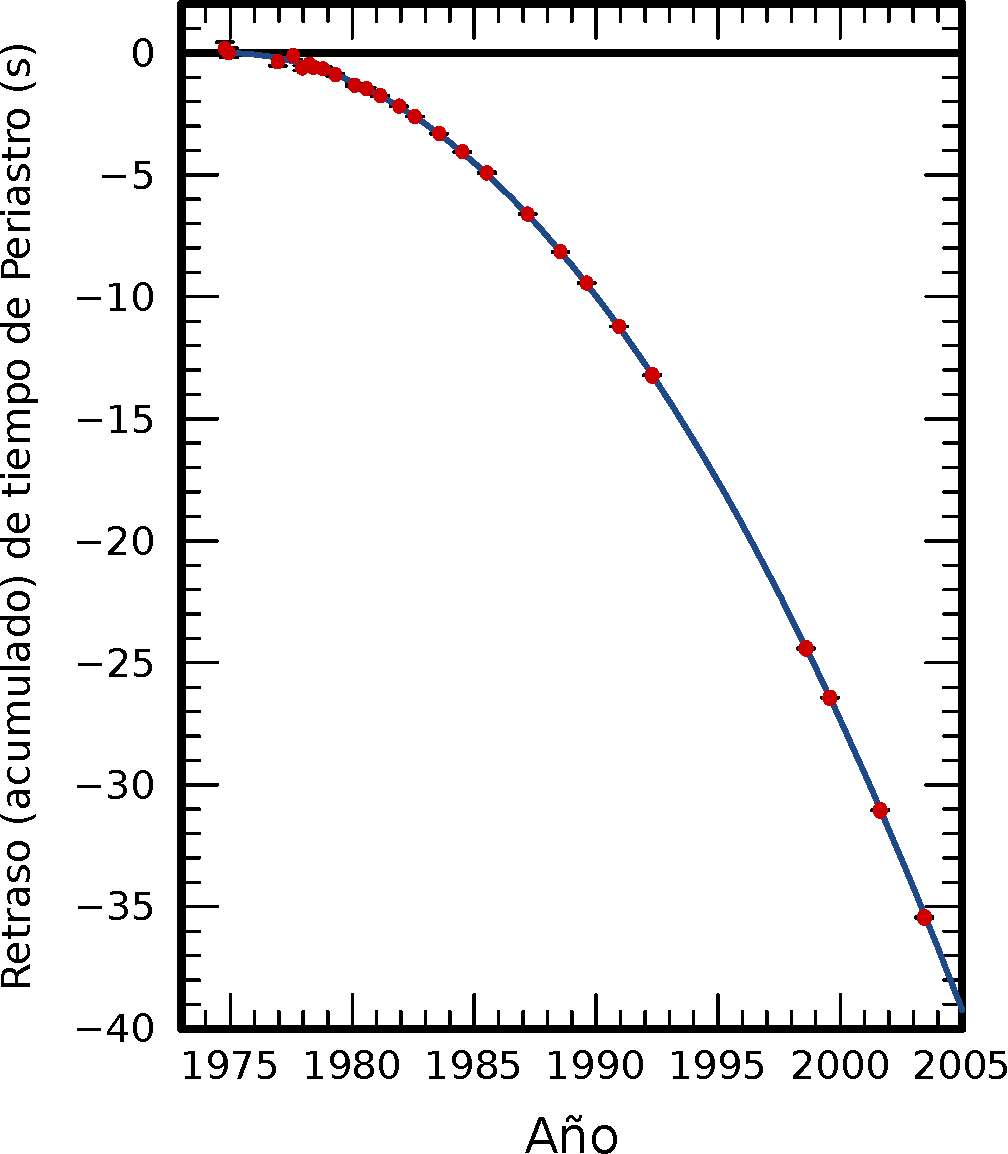
\psfig{file=fig/fig-HT.pdf,height=7cm,angle=0}}
\caption{Predicci'on y observaci'on del tiempo en que el pulsar binario de Hulse y Taylor completa cada revolución (tiempo de periastro), respecto al valor newtoniano. Adaptada a partir de \href{http://en.wikipedia.org/wiki/File:PSR_B1913\%2B16_period_shift_graph.svg}{esta} figura original.}
\label{fig:HT}
\end{figure}
\end{center}


\begin{align}
\frac{da}{dt} &= -\frac{64}{5}\frac{G^3\mu M^2}{c^5a^3}\frac{1}{\left(1-e^2\right)^{7/2}}\left(1+\frac{73}{24}e^2+\frac{37}{96}e^4\right) \label{dadt},\\
\frac{de}{dt} &= -\frac{304}{15}\frac{G^3\mu M^2}{c^5a^4}\frac{e}{\left(1-e^2\right)^{5/2}}\left(1+\frac{121}{304}e^2\right). \label{dedt}
\end{align}

En el caso de una 'orbita circular, $e=0$, la ecuaci'on se reduce a
\begin{equation}
\frac{da}{dt} = -\frac{64}{5}\frac{G^3\mu M^2}{c^5a^3},
\end{equation}
cuya soluci'on es...
\begin{equation}
a(t) = \left[a_0^4-\frac{256}{5}\frac{G^3\mu M^2}{c^5}(t-t_0)\right]^{1/4}.
\end{equation}

Dividiendo las ecuaciones \eqref{dadt} \eqref{dedt} para $\dot{a}$ y $\dot{e}$ podemos eliminar el tiempo de estas expresiones y encontrar una ecuaci'on que relaciona directamente $a$ con $e$:
\begin{equation}
\frac{da}{de}=\frac{12}{19}a\frac{1+(73/24)e^2+(37/96)e^4}{e(1-e^2)[1+(121/304)e^2]}.
\end{equation}
La soluci'on de esta ecuaci'on es de la forma
\begin{equation}
a(e)=a_{0}\frac{g(e)}{g(e_{0})},
\end{equation}
con 
\begin{equation}
g(e):= \frac{e^{12/19}}{1-e^2}\left(1+\frac{121}{304} \right)^{870/2299}.
\end{equation}

% \section{Ecuaci'on de movimiento para una part'icula de prueba}
%
% \begin{equation}
% \frac{d^2x^I}{dt^2}=-\Gamma^I_{\ 00}+ \left[\Gamma^0_{\ 00}\delta^I_J-
% 2\Gamma^I_{\ 0J}\right]v^J +\left[2 \Gamma^0_{\ 0J}\delta^I_K -
% \Gamma^I_{\ JK}\right]v^Jv^K + \Gamma^0_{\ JK}v^Iv^Jv^K ,
% \end{equation}
%
% A primer orden en $v$, es decir, en el l'imite no-relativista, podemos
% escribir
%
% \chapter{La apr'oximaci'on post-newtoniana}
%
% The post-Newtonian approximation (see \cite{Wei72,Will93}, also \cite{Sch96})
% applies to systems of slowly moving particles bound together by
% gravitational forces. In such systems the typical values of the Newtonian
% potential $\bar{\phi}\sim\frac{G\bar{M}}{\bar{r}}$
% ($\bar{M}$ and $\bar{r}$ are the typical mass and distance between
% particles) is of the same
% order of magnitude as the typical squared velocities of the particles
% $\bar{v}^2$ (e.g. for a test particle in a circular orbit of radius $r$
% around a central mass $M$ we actually have $v^2=GM/r$).
% The post-Newtonian approximation is based on an expansion of
% the quantities involved in the determination of the trajectories of the
% particles, in powers of the small parameter $v$, taking into account
% that $O(\phi)\sim O(v^2)$, and keeping only the first post-Newtonian
% correction in a consistent way. In this section we follow the conventions
% and notation of Weinberg \cite{Wei72} and use $c=1$, and a metric with
% signature $(-,+,+,+)$.
%
% The geodesic equation for a test particle can be written as (see
% \cite{Wei72}, eq. (9.1.2))
% \begin{equation}\label{geo}
% \frac{d^2x^i}{dt^2}=-\Gamma^i_{\ 00}-2\Gamma^i_{\ 0j}v^j -
% \Gamma^i_{\ jk}v^jv^k +\left[\Gamma^0_{\ 00} +2 \Gamma^0_{\ 0j}v^j +
% \Gamma^0_{\ jk}v^jv^k\right]v^i \, es decir,
% \end{equation}
% where we are using coordinates $x^\mu=(t,x^i)$, $i=1,2,3$,
% $v^i:=\frac{dx^i}{dt}$ and $\Gamma^\mu_{\ \nu\lambda}$ are the
% Christoffel symbols corresponding to the metric tensor $g$
% describing the gravitational field of the system.
%
% In the Newtonian approximation, one neglects all velocities and identifies
% $g_{00}\approx -1-2\phi$ so that one recovers the Newtonian law
% \begin{equation}\label{na}
% \frac{d^2x^i}{dt^2}=-\Gamma^i_{\ 00}\approx \frac{1}2\,\delta^{ij}
% \frac{\partial g_{00}}{\partial x^j}\approx -\delta^{ij}
% \frac{\partial \phi}{\partial x^j} .
% \end{equation}
% One then sees that (\ref{na}) contains only terms from (\ref{geo}) up
% to order $v^2/r$. Therefore, in the post-Newtonian approximation, one wants
% to compute (\ref{geo}) up to the next order, which in this case corresponds
% to order $v^4/r$. To carry out this procedure one consider the derivatives
% $\frac{\partial}{\partial x^i}$ and $\frac{\partial}{\partial t}$ as of
% order $1/r$ and $v/r$ respectively.
%
% One can see from (\ref{geo}) that one needs to know the Christoffel
% symbols to the following orders of accuracy: $\Gamma^i_{\ 00}$ to order
% $v^4/r$, $\Gamma^i_{\ 0j}$ to order $v^3/r$, $\Gamma^i_{\ jk}$ to order
% $v^2/r$, $\Gamma^0_{\ 00}$ to order $v^3/r$, $\Gamma^0_{\ 0j}$ to order
% $v^2/r$ and $\Gamma^0_{\ jk}$ to order $v/r$.
% For that, it is enough to compute the metric tensor to the following orders:
% $g_{00}$ to order $v^4$, $g_{0i}$ to order $v^3$ and $g_{ij}$ to order $v^2$.
% In this way, one uses expansions of the form
% \begin{eqnarray}
% g_{00}&=&-1+\stackrel{(2)}g_{00} + \stackrel{(4)}g_{00} + \dots \, es decir,
% \\
% g_{0i}&=&\stackrel{(3)}g_{0i} + \dots \, es decir, \\
% g_{ij}&=&\delta_{ij}+\stackrel{(2)}g_{ij} + \dots \, .
% \end{eqnarray}
%
% With this expansion and a similar one for the matter energy-mom'entum tensor,
% i.e.
% \begin{eqnarray}
% T^{00}&=&\stackrel{(0)}{T^{00}} + \stackrel{(2)}{T^{00}}+ \dots \, es decir,
% \\
% T^{0i}&=&\stackrel{(1)}{T^{0i}} + \stackrel{(3)}{T^{0i}}+ \dots \, es decir,
% \\
% T^{ij}&=&\stackrel{(2)}{T^{ij}} + \stackrel{(4)}{T^{ij}}+ \dots \, es decir,
% \end{eqnarray}
% one can develop the Einstein eqs.
% \begin{equation}
% R_{\mu\nu}=-8\pi G\left(T_{\mu\nu}-\frac{1}2\, g_{\mu\nu}T^\lambda_{\
% \lambda} \right)\, es decir,
% \end{equation}
% in order to obtain equations for the functions entering in the expansion of
% the metric coefficients. A great simplification is achieved by using
% coordinates satisfying the harmonic coordinate condition
% $g^{\mu\nu}\Gamma^\lambda_{\ \mu\nu}=0$. With this coordinate gauge, the
% Einstein equations reduce to \cite{Wei72}:
% \begin{eqnarray}
% \nabla^2 \stackrel{(2)}g_{00}&=&-8\pi G \stackrel{(0)}{T^{00}} \, es decir, \\
% \nabla^2 \stackrel{(4)}g_{00}&=& \frac{\square \stackrel{(2)}g_{00}}
% {\partial t^2} + \stackrel{(2)}g_{ij}\frac{\square \stackrel{(2)}g_{00}}
% {\partial x^i \partial x^j} - \left(\frac{\partial \stackrel{(2)}g_{00}}
% {\partial x^i}\right) \left(\frac{\partial \stackrel{(2)}g_{00}}
% {\partial x^i}\right) \nonumber \\
% && - 8\pi G\left[\stackrel{(2)}{T^{00}}- 2\stackrel{(2)}g_{00}
% \stackrel{(0)}{T^{00}} + \stackrel{(2)}{T^{ii}}\right] \, es decir, \\
% \nabla^2 \stackrel{(3)}g_{0i}&=&+16\pi G \stackrel{(1)}{T^{0i}} \, es decir,
% \\
% \nabla^2 \stackrel{(2)}g_{ij}&=&-8\pi G \delta_{ij}\stackrel{(0)}{T^{00}} .
% \end{eqnarray}
% The solution of these equations is given by
% \begin{eqnarray}
% \stackrel{(2)}g_{00}&=&-2\phi \, es decir, \\
% \stackrel{(4)}g_{00}&=&-2\phi^2 -2\psi \, es decir, \\
% \stackrel{(3)}g_{0i}&=&\xi_i \, es decir, \\
% \stackrel{(2)}g_{ij}&=&-2\delta_{ij}\phi \, es decir,
% \end{eqnarray}
% where
% \begin{eqnarray}
% \phi&:=&-G\int d^3 x^\prime \frac{\stackrel{(0)}{T^{00}}({\bf x}^\prime,t)}
% {\left|\bf x-x^\prime\right|} ,\\
% \psi&:=&-\int \frac{d^3 x^\prime}{\left|\bf x-x^\prime\right|}\left[
% \frac{1}{4\pi}\, \frac{\square \phi({\bf x}^\prime,t)}{\partial t^2} +
% G \stackrel{(2)}{T^{00}}({\bf x}^\prime,t)+G\stackrel{(2)}{T^{ii}}
% ({\bf x}^\prime,t) \right], \\
% \xi_i&:=&-4G\int d^3 x^\prime \frac{\stackrel{(1)}{T^{0i}}({\bf x}^\prime,t)}
% {\left|\bf x-x^\prime\right|} .
% \end{eqnarray}
%
%
% In summary, in the post-Newtonian approximation the metric tensor is given by
% \begin{eqnarray}
% g_{00}&=&-1 -2\phi -2\phi^2 -2\psi + O(v^6),\\
% g_{0i}&=&\xi_i + O(v^5),\\
% g_{ij}&=&\delta_{ij}\left(1-2\phi\right) +O(v^4)\, .
% \end{eqnarray}
% The geodesic eq. (\ref{geo}) in vector notation takes the form
% (see \cite{Wei72}, eq. (9.2.1)):
% \begin{eqnarray}
% \frac{d\vec{v}}{dt}&=&-\vec{\nabla}\left(\phi +2\phi^2+\psi\right)
% -\frac{\partial\vec{\xi}}{\partial t} + \vec{v}\, \times\left(\vec{\nabla}
% \times \vec{\xi}\right) \nonumber \\
% && + 3\vec{v}\, \frac{\partial\phi}{\partial t}+4\vec{v}
% \left(\vec{v}\cdot\vec{\nabla}\right)\phi -v^2\vec{\nabla}\phi +O(v^6/r) \, .
% \end{eqnarray}
%
% \section{Static, spherically symmetric pressureless matter distribution}
%
% %For the case of a static, spherically symmetric matter distribution we have
% %$T^{00}=T^{00}(r)$ and $T^{0i}=0$.
%
% We assume a static, spherically symmetric matter distribution described
% by the energy mom'entum tensor of dust, so that
% \begin{equation}
% T^{\mu\nu}=\rho\, U^\mu U^\nu\, es decir,
% \end{equation}
% with $U^\mu=\left(\frac{dt}{d\tau},0,0,0\right)$ is the 4-velocity of
% the static matter distribution and $\rho=\rho(r)$ is the rest mass density.
% In this case only $T^{00}$ is different from zero and, in particular :
% %(\cite{Wei72}, eqs. (9.3.8)- (9.3.11)):
% \begin{eqnarray}
% \stackrel{(0)}{T^{00}}&=&\rho(r) , \\
% \stackrel{(2)}{T^{00}}&=& -2\phi(r)\, \rho(r) \, . \label{dif}
% \end{eqnarray}
%
% %[Now I have obtained the factor 2, in agreement with Will, table 4.1, with
% %$U=-\phi$ and $\Phi_2=-\psi/2$. See also eq. (39.42a) in \cite\cite{MTW73}
%.Now everything seems to be correct.]
%
% Under these simplifications the metric is given by
% \begin{eqnarray}
% g_{00}&=&-1 -2\phi -2\phi^2 -2\psi + O(v^6),\\
% g_{0i}&=&0 + O(v^5),\\
% g_{ij}&=&\delta_{ij}\left(1-2\phi\right) +O(v^4)\, es decir,
% \end{eqnarray}
% with
% \begin{eqnarray}
% \phi&:=&-G\int d^3 x^\prime \frac{\rho(r^\prime)}
% {\left|\bf x-x^\prime\right|} \, es decir, \\
% \psi&:=&2G\int \frac{d^3 x^\prime}{\left|\bf x-x^\prime\right|} \,
% \phi(r^\prime)\, \rho(r^\prime) \, .
% \end{eqnarray}
%
% The geodesic equation reduces to
% \begin{equation}
% \frac{d\vec{v}}{dt}=-\vec{\nabla}\left(\phi +2\phi^2+\psi\right)
% +4\vec{v}\left(\vec{v}\cdot\vec{\nabla}\right)\phi -v^2\vec{\nabla}\phi
% +O(v^6/r) \, .
% \end{equation}
%
% For a finite matter distribution the potentials $\phi$ and $\psi$ approach
% to zero at infinity. Therefore, the metric is asymptotically the Minskowski
% metric. One then sees, that at infinity, the coordinates employed become
% inertial coordinates. As a result, the associated reference frame at infinity
% is an inertial frame in which the central matter distribution seems to be at
% rest. This corresponds, to an inertial frame comoving with the central mass
% distribution (the center of the galaxy in our case).
%
% However, for a isolated matter distribution, the metric tensor is given
% asymptotically by
% \begin{eqnarray}
% g_{00}&=&-1 +2\frac{G\stackrel{0}{M}}{r} + 2\frac{G\stackrel2{M}}{r}
% + O(r^{-2},v^6),\\
% g_{0i}&=&0 + O(v^5),\\
% g_{ij}&=&\delta_{ij}\left(1+2\frac{G\stackrel{0}{M}}{r}\right)
% +O(r^{-2},v^4)\, es decir,
% \end{eqnarray}
% where
% \begin{equation}
% \stackrel{0}{M}:=\int d^3 x\, \rho ,
% \qquad \stackrel2{M}:=-2\int d^3 x\, \rho\phi \, .
% \end{equation}
%
% Since it is the ``total gravitating mass" $M:=\stackrel{0}{M}+
% \stackrel2{M}$ the one of practical interest (the one
% obtained by studying the motion of test particles far from the central body),
% it is more convenient to replace the rest mass density $\rho$
% in the above equations by the
% ``gravitational mass density" $\rho_g:=\rho\left( 1-
% 2\phi\right)$,
% so that to first post-newtonian order, we can write
% \begin{eqnarray}
% g_{00}&=&-1 -2\phi_g -2\phi_g^2 + O(v^6),\\
% g_{0i}&=&0 + O(v^5),\\
% g_{ij}&=&\delta_{ij}\left(1-2\phi_g\right) +O(v^4)\, es decir,
% \end{eqnarray}
% where
% \begin{equation}
% \phi_g:=-G\int d^3 x^\prime \frac{\rho_g(r^\prime)}
% {\left|\bf x-x^\prime\right|}=\phi+\psi \, .
% \end{equation}
%
% The geodesic eq. then reads,
% \begin{equation}\label{geopn}
% \frac{d\vec{v}}{dt}=-\vec{\nabla}\left(\phi_g +2\phi_g^2\right)
% +4\vec{v}\left(\vec{v}\cdot\vec{\nabla}\right)\phi_g -v^2\vec{\nabla}
% \phi_g +O(v^6/r) \, .
% \end{equation}
%
% In newtonian terms, this procedure can be thought as a mass renormalization.
% In this context, the total gravitating mass of the system
% ($M=\stackrel{0}{M}+\stackrel2{M}=\int d^3 x\, \rho_g$,
% defined asymptotically) has a contributions from the ``gravitational
% energy'' of the system. Thus, the problem of
% phenomenologically modelling the density $\rho$ is replaced now by the
% problem of modelling $\rho_g$. Since in the applications, we will always use
% this last form of the geodesic equations, we will omit the subindex in
% $\phi_g$ and $\rho_g$ and denote them simply by $\phi$ and $\rho$.
%
% \section{Energy and Angular mom'entum}
%
% It is possible to define the post-Newtonian generalizations of the
% {\em conserved} quantities corresponding to energy and mom'entum
% per unit mass in the Newtonian theory.
%
% We define:
% \begin{eqnarray}
% E&:=&\frac{1}2 v^2 + \phi -3\phi v^2 -\phi^2
% %+\psi
% \, es decir, \\
% \vec{l}&:=&(1-4\phi)\, \vec{r}\times\vec{v} \, .
% \end{eqnarray}
%
% Using the equation of motion \ref{geopn}) one shows that these quantities are
% conserved within our approximation:
% \begin{equation}
% \frac{dE}{dt}=0 +O(v^7/r), \qquad \frac{d\vec{l}}{dt}=\vec{0} + O(v^6) \,.
% \end{equation}
%
% In the orbit plane, one can use cylindrical coordinates $(r,\varphi)$
% \footnote{As usual $x=r\cos(\varphi)$, $y=r\sen(\varphi)$} and
% find the equation giving the dependence of the angle $\varphi$ in terms of
% $r$. Using the expressions for the conserved quantities in cylindrical
% coordinates, namely
% \begin{eqnarray}
% E&=&\frac{1}2\left(1-6\phi\right)\left[\left(\frac{dr}{dt}\right)^2 +
% r^2 \left(\frac{d\varphi}{dt}\right)^2\right] + \phi -2\phi^2
% %+\psi
% \, es decir, \\
% l&=&\left(1-4\phi\right)\, r^2 \frac{d\varphi}{dt} \, es decir,
% \end{eqnarray}
% one finds
% \begin{equation}
% \frac{l^2}{r^4}\left(\frac{dr}{d\varphi}\right)^2=2(1-2\phi)E-\frac{l^2}{r^2}
% -2\phi +6\phi^2 %-\psi
% +O(v^6) \, .
% \end{equation}
% Thus, one obtains
% \begin{equation}\label{fideere}
% \frac{d\varphi}{dr}=\pm \frac{l}{r^2}\left[2(1-2\phi)E-\frac{l^2}{r^2}
% -2\phi +6\phi^2 %-\psi
% \right]^{-1/2} \, .
% \end{equation}
%




\chapter{Elementos de Cosmolog'ia ***PRELIMINAR***}\label{cap:cosmo}
El objetivo de la cosmolog'ia es describir la estructura y din'amica del universo a muy grandes escalas ($\gtrsim 10^{7}\text{pc}$, $1\text{pc}\approx 3.26\text{ly}\approx 3.1\times 10^{16}\text{m}$). A estas escalas cosmol'ogicas, la din'amica de los constituyentes del universo es gobernada por la interacci'on gravitacional, que es descrita satisfactoriamente (hasta donde sabemos) por la teor'ia de RG.
Com'unmente, muchas consideraciones de simplicidad son usadas en la formulaci'on de los modelos cosmol'ogicos. 
En primer lugar el contenido de materia/energ'ia en el Universo es usualmente modelado como un fluido perfecto, 
con densidad propia $\rho$ y presi'on $p$, y donde cada elemento de fluido representa una regi'on del espacio de m'as de $10^{7}\text{pc}$. Adem'as, el modelo cosmol'ogico est'andar asume que a escalas cosmol'ogicas el Universo es \textit{is'otropo y homog'eneo}. Estas consideraciones de simplicidad son usualmente llamadas \textit{principio cosmol'ogico}. El requerimiento de isotrop'ia significa que la distribuci'on de materia y energ'ia en el Universo, respecto a observadores com'oviles con el fluido cosmol'ogico, es la misma en todas las direcciones, asumiendo que los elementos del fluido cosmol'ogico (c'umulos de galaxias) se mueven por geod'esicas del espaciotiempo.
La supuesta homog'eneidad significa que la distribuci'on de materia y energ'ia del Universo es la misma en todos los puntos de 'este (a un mismo tiempo de evoluci'on cosmol'ogica), es decir, que no existe punto f'isicamente privilegiado en el 
Universo. Esto implica que las propiedades geom'etricas del espacio en un punto deben ser las mismas que en cualquiera otro a un mismo tiempo cosmol'ogico.
La mejor evidencia observacional a favor del principio cosmol'ogico la ofrece la radiaci'on c'osmica de fondo (CMB), descubierta en 1965 (Penzias y Wilson) que, de acuerdo a las mediciones realizadas, es altamente is'otropa (con anisotrop'ias del orden de una parte en $10^5$).
\section{Espacios de Curvatura constante}
Sabemos que el espacio eucl'ideo tridimensional es invariante bajo rotaciones y translaciones, es decir, es is'otropo y homog'eneo. Esto lo hace un buen candidato para caracterizar la parte espacial del universo a grandes escalas. Por otro lado, el espacio eucl'ideo tiene curvatura igual a cero en toda su extensi'on y nos restringe al caso en que el universo es espacialmente plano. Existen, sin embargo, espacios tridimensionales is'otropos y homog'eneos de curvatura no nula. Una forma de encontrar la m'etrica de estos espacios es generalizando la construcci'on de espacios bidimensionales is'otropos y homog'eneos, que describimos a continuaci'on.

Consideremos el espacio eucl'ideo tridimensional cuyo elemento de l'inea en coordenadas cartesianas es:
\begin{equation}
dl^{2}= dx^{2} + dy^{2} + dz^{2}.
\end{equation}
Ahora nos restingimos s'olo a los puntos sobre una esfera\footnote{Es claro que se conserva la homogeneidad y la isotrop'ia pues una esfera es invariante bajo rotaciones.} de radio $a$. El elemento de l'inea inducido sobre la esfera puede escribirse, en t'erminos de las coordenadas $x$ e $y$, como
\begin{equation}
dl^{2}= dx^{2} + dy^{2} + \frac{(xdx + ydy)^{2}}{a^2-(x^2 + y^2)},
\end{equation}
donde hemos usado la condici'on $x^2 +y^2 + z^2 =a^2$ para eliminar la coordenada $z$.

An'alogamente podemos generar otra superficie is'otropa y homog'enea considerando un espacio tridimensional ``Lorentziano", con elemento de l'inea
\begin{equation}
dl^{2}= dx^{2} + dy^{2}  -dz^{2},
\end{equation}
y luego restringui'endonos a la superficie determinada por la condici'on $z^2-x^2-y^2=a^2$ (superficie hiperb'olica), obteni'endose
\begin{equation}
dl^{2}= dx^{2} + dy^{2} - \frac{(xdx + ydy)^{2}}{a^2+(x^2 + y^2)}.
\end{equation}

En resumen, podemos escribir\footnote{Usando el elemento de l'inea $dl^{2}= dx^{2} + dy^{2} + kdz^{2}$ y adem'as $z^2 +k(x^2 + y^2)=a^2$.}
\begin{equation}
dl^{2}= dx^{2} + dy^{2} + k\frac{(xdx + ydy)^{2}}{a^2-k(x^2 + y^2)},\label{60j}
\end{equation}
con
\begin{equation}
k=\left\{\begin{array}{rl}
-1,& \mbox{Superficie Hiperb\'olica}\\ \label{61j}
0,& \mbox{Superficie Plana}\\
1,& \mbox{Superficie Esf\'erica}
\end{array}\right. .
\end{equation}
Estas tres superficies poseen curvatura constante. En efecto, las componentes no nulas de la conexi'on en estas coordenadas son:
\begin{align}
\Gamma^{1}_{11} &= \frac{{k}^{2}\,x\,{y}^{2}-a^{2}\,k\,x}{a^{2}\,k\,{y}^{2}+a^{2}\,k\,{x}^{2}-a^{4}}, \quad
\Gamma^{2}_{11}=\frac{{k}^{2}\,{y}^{3}-a^{2}\,k\,y}{a^{2}\,k\,{y}^{2}+a^{2}\,k\,{x}^{2}-a^{4}}, \\
\Gamma^{1}_{12} &= \frac{-{k}^{2}\,{x}^{2}\,y}{a^{2}\,k\,{y}^{2}+a^{2}\,k\,{x}^{2}-a^{4}},\quad
\Gamma^{2}_{12}=\frac{-{k}^{2}\,x\,{y}^{2}}{a^{2}\,k\,{y}^{2}+a^{2}\,k\,{x}^{2}-a^{4}},\\
\Gamma^{1}_{22} &= \frac{{k}^{2}\,{x}^{3}-a^{2}\,k\,x}{a^{2}\,k\,{y}^{2}+a^{2}\,k\,{x}^{2}-a^{4}}, \quad
\Gamma^{2}_{22}=\frac{\left( {k}^{2}\,{x}^{2}-a^{2}\,k\right) \,y}{a^{2}\,k\,{y}^{2}+a^{2}\,k\,{x}^{2}-a^{4}},
\end{align}
y entonces el escalar de curvatura es dado por
\begin{equation}
R=\frac{2k}{a^2}.
\end{equation}
Puede verificarse adem'as que estos espacios son \textbf{maximalmente sim'etricos}, ya que poseen el n'umero m'aximo de 3 vectores de Killing independientes permitidos por la dimensi'on.
Puede elegirse como vectores de Killing independientes a
\begin{equation}
\hat{\xi}_{1}=\sqrt{1-k(x^2+y^2)}\partial_x, \qquad \hat{\xi}_{2}=\sqrt{1-k(x^2+y^2)}\partial_y, \qquad \hat{\xi}_{3} = x\partial_y -y\partial_x.
\end{equation}

\section{La m'etrica de Friedman-Lema\^itre-Robertson-Walker}
Propuesta 1922 por \href{http://es.wikipedia.org/wiki/Aleksandr_Fridman}{Alexander Friedman} la m'etrica de Friedman-Lema\^itre-Robertson-Walker (FLRW) fue redescubierta en 1930 por \href{http://en.wikipedia.org/wiki/Howard_P._Robertson}{Howard Robertson} y \href{http://en.wikipedia.org/wiki/Arthur_Geoffrey_Walker}{Arthur G. Walker}, quienes la hicieron famosa y por lo mismo lleva sus nombres. Esta m'etrica describe un Universo en expansi'on (o contracci'on), espacialmente homog'eneo e is'otropo.

An'alogamente con la secci'on anterior buscamos una m'etrica que describa un espaciotiempo cuya parte espacial sea is'otropa y homogenea. Partimos de un espacio plano ficticio de dimensi'on 5,
\begin{equation}
 ds^{2}= c^2dt^2 -(dx^{1})^{2}-(dx^{2})^{2}-(dx^{3})^{2}-k(dx^{4})^{2},
 \end{equation}
para luego restringirnos a la hipersuperficie definida por la condici'on:
 \begin{equation}\label{60k}
(x^{4})^{2} +kx^{i}x^{i}=a^{2}(t),\qquad i=1,2,3, 
  \end{equation}
donde $k$ puede adoptar los valores -1,0 'o 1. Obteniendo una expresi'on an'aloga a \eqref{60j} para la m'etrica inducida:
\begin{equation}\label{60kk}
ds^{2}= c^2dt^2 - d\vec{x}^{2} - k\frac{(\vec{x}\cdot d\vec{x})^{2}}{a^{2}(t)+k\vec{x}^{2}}. 
\end{equation}

Por otro lado, dado que nuestra hipersuperficie satisface (\ref{60k}) podemos reescalar la parte espacial, usando
$x^i=a(t)x'^{i}$,  tal que
\begin{equation}
(x'^{4})^{2} +kx'^{i}x'^{i}=1,
\end{equation}
Luego (\ref{60kk}) adopta la forma
\begin{equation}
ds^{2}= c^2dt^2 - a^{2}(t)\left[ d\vec{x}'^{2}+ k\frac{(\vec{x}'\cdot d\vec{x}')^{2}}{1-k\vec{x}'^{2}}\right],
\end{equation}
donde $a(t)$ es un factor de escala con dimensiones de longitud, dependiente s'olo de la coordenada temporal $t$, conocido
como el \textit{Factor de Escala Cosmol'ogico}.\\
Finalmente renombrando $x'^i$ como $x^i$ obtenemos la expresi'on
\begin{equation}
ds^{2}= c^2dt^2 - a^{2}(t)\left[ d\vec{x}^{2} + k\frac{(\vec{x}\cdot d\vec{x})^{2}}{1-k\vec{x}^{2}}\right].
\end{equation}
Otra foma com'un de expresar el intervalo es usando coordenadas esf'ericas:
\begin{equation}\marginnote{M'etrica de FRW}
 ds^2=c^2dt^2-a^2(t)\left[\frac{dr^2}{1-kr^2}+r^2\,d\theta^2+r^2\sen^2\theta\,d\varphi^2\right].\label{dsFRW}
\end{equation}
La constante $k$ puede adoptar, al igual que en (\ref{61j}), los valores $0$, $1$ 'o $-1$, y est'a relacionada con la curvatura nula, positiva o
negativa, de la secci'on espacial ($t=$ cte.), respectivamente.\\
En efecto, la geometr'ia espacial est'a determinada por el elemento de l'inea
\begin{equation}
 d\ell^2=a^2(t)\left[\frac{dr^2}{1-kr^2}+r^2\,d\theta^2+r^2\sen^2\theta\,d\varphi^2\right],
\end{equation}
cuyo escalar de curvatura es constante (su valor es independiente de $r$, $\theta$ y $\varphi$) e igual a $6k/a^2$.
Claramente, si $k=0$ la geometr'ia espacial es plana. Si $k=-1$ entonces el escalar de curvatura es negativo. En ambos 
casos el espacio es \textit{abierto}, en el sentido que la coordenada $r$ puede variar entre $0$ y $+\infty$. Si $k=+1$ 
entonces el espacio es \textit{cerrado}, ya que $r$ puede variar entre $0$ y $+1$, y el volumen total es finito.
%\begin{equation}
%R^{(3)}_{ijkl}=\frac{k}{a^2}\left(g^{(3)}_{ik}g^{(3)}_{jl}-g^{(3)}_{jk}g^{(3)}_{il}\right).
%\end{equation}
%\subsection{Otros sistemas de coordenadas}
%Coordenadas hyperesf'ericas $(\chi,\theta,\varphi)$
%\begin{equation}
%r=S_k(\chi):=\left\{\begin{array}{ll}
%\frac{1}{\sqrt{k}}\sen(\sqrt{k}\chi),& k>0\\
%r, & k=0\\
%\frac{1}{\sqrt{|k|}}\senh(\sqrt{|k|}\chi), & k<0
%\end{array}\right.
%\end{equation}
%\begin{equation}
%d\ell^2=a^2\left[d\chi^2+S_k^2(\chi)\,d\Omega^2\right]
%\end{equation}

%Coordenadas esf'ericas conformes $(\rho,\theta,\varphi)$
%\begin{equation}
%r=\frac{\rho}{1+k\rho^2/4}
%\end{equation}
%\begin{equation}
%d\ell^2=\frac{a^2}{\left(1+k\rho^2/4\right)^2}\left[d\rho^2+\rho^2\,d\Omega^2\right]
%\end{equation}

%Coordenadas cartesianas conformes $(x,y,z)$
%\begin{equation}
%d\ell^2=\frac{a^2}{\left(1+k\vec{x}^2/4\right)^2}\left[dx^2+dy^2+dz^2\right]
%\end{equation}
\section{Observadores com'oviles}
Las componentes no nulas de la conexi'on en las coordenadas en las que el elemento de l'inea es dado por (\ref{dsFRW}) son
\begin{eqnarray} 
 \Gamma^0_{11}&=&\frac{1}{c}\frac{a\dot{a}}{1-kr^2}, \qquad \Gamma^0_{22}=\frac{1}{c}a\dot{a}r^{2}, \qquad 
\Gamma^0_{33}=\frac{1}{c}a\dot{a}r^2\sen^2\theta ,\\
\Gamma^1_{01}&=&\frac{1}{c}\frac{\dot{a}}{a}, \qquad \Gamma^1_{11}=\frac{kr}{1-kr^2}, \qquad
\Gamma^1_{22}=-r(1-kr^2),\\
 \Gamma^1_{33}&=&-r(1-kr^2)\sen^2\theta, \qquad \Gamma^2_{02}=\frac{1}{c}\frac{\dot{a}}{a}, \qquad
\Gamma^2_{12}=\frac{1}{r}, \\
\Gamma^2_{33}&=&-\sen\theta\cos\theta, \qquad \Gamma^3_{03}=\frac{1}{c}\frac{\dot{a}}{a}, \qquad
\Gamma^3_{13}=\frac{1}{r}, \qquad
\Gamma^3_{23}=\cot\theta .
\end{eqnarray}
Ya que $\Gamma^\mu_{00}=0$ la l'inea de mundo $x^\mu(\tau)=(c(\tau-\tau_0),r_0,\theta_0,\varphi_0)$ con $\tau_0$, $r_0$, $\theta_0$ y $\varphi_0$ constantes es una geod'esica. En efecto,
\begin{equation}
\frac{dx^\mu}{d\tau}=(c,0,0,0), \qquad   \frac{d^2x^\mu}{d\tau^2}=0,
\end{equation}
y por lo tanto se satisface la ecuaci'on de la geod'esica,
\begin{equation}
 \frac{d^2x^\mu}{d\tau^2}+\Gamma^\mu_{\ \nu\lambda}\frac{dx^\nu}{d\tau}\frac{dx^\lambda}{d\tau}=0+\Gamma^\mu_{\ 00}c^2=0.
\end{equation}
Los c'umulos de galaxias (o el ``fluido cosmol'ogico'') se mueven en geod'esicas de la m'etrica cosmol'ogica,
que se identifican con aquellas con coordenadas espaciales constantes. De esta forma, (\ref{dsFRW}) implica que los
intervalos de coordenada temporal $t$ coinciden con los intervalos de tiempo propio respecto a part'iculas del fluido
cosmol'ogico. Por esta raz'on $t$ es llamado \textit{tiempo c'osmico} y las coordenadas espaciales $(r,\theta,\varphi)$
son \textit{com'oviles} con el fluido cosmol'ogico.
\section{Redshift Cosmol'ogico}
Consideremos un observador $O$ movi'endose con el fluido cosmol'ogico. Sin p'erdida de generalidad (debido a la
homogeneidad del espacio) podemos elegir las coordenadas espaciales de $O$ de modo que $r_O=0$. Adem'as, consideramos 
otra part'icula de fluido cosmol'ogico con coordenadas $(r_1,\theta_1,\varphi_1)$, que emite una se\~nal luminosa en el
evento con tiempo c'osmico $t_1$ hacia $O$, quien recibe la se\~nal en $t=t_0$. La se\~nal luminosa viaja hasta $O$ por 
una curva geod'esica nula con $d\theta=d\varphi=0$. De (\ref{dsFRW}) vemos que la condici'on $ds^2=0$ implica:
\begin{equation}
\frac{cdt}{a(t)}=-\frac{dr}{\sqrt{1-kr^2}}. \label{59i}
\end{equation}
Integrando (\ref{59i}) encontramos que
\begin{equation}
c\int_{t_1}^{t_0}\frac{dt}{a(t)}=-\int_{r_1}^{0}\frac{dr}{\sqrt{1-kr^2}}=:f(r_1), \label{60i}%
\end{equation}
donde
\begin{equation}
f(r_1)=\left\{
\begin{array}
[c]{ccl}%
\text{arcsen}(r_1), &\text{si}& k=+1\\
r_1, &\text{si}& k=0\\
\text{arcsenh} (r_1), &\text{si}& k=-1
\end{array}
\right. . \label{61i}%
\end{equation}
Vemos que la expresi'on (\ref{60i}) que, dados $a(t)$, $r_1$, $t_1$ y $k$ puede entenderse como 
una ecuaci'on para $t_0$, el tiempo cosmol'ogico de recepci'on de la se\~nal. Si, por ejemplo, $a(t)=a(t_1)$ es 
constante entonces $t_1=t_0+a(t_1)f(r_1)/c$. Si $\dot{a}>0$ entonces $t_1>t_0+a(t_1)f(r_1)/c$ y si $\dot{a}<0$ 
entonces $t_1<t_0+a(t_1)f(r_1)/c$. Este comportamiento corresponde a la noci'on cl'asica que cada elemento de 
fluido cosmol'ogico (si bien sus coordenadas espaciales permanecen constantes) se aleja o acerca respecto a cualquier 
otro, es decir que el Universo se expande o contrae, dependiendo de si el factor de escala $a(t)$ aumenta o disminuye, 
respectivamente.
Ahora, consideremos dos rayos de luz sucesivos emanando de $P$ a tiempos
$t_1$ y $t_1+\Delta t_1$, y recibidos por $O$ en los tiempos $t_0$ y
$t_0+\Delta t_0$ respectivamente, asumiendo que tanto el emisor como el receptor  de la se\~nal permanecen en sus
mismas posiciones. \textbf{Entonces, usando (\ref{60i}) podemos escribir:}
\begin{equation}
c\int_{t_1+\Delta t_1}^{t_0+\Delta t_0}\frac{dt}{a(t)}=-\int_{r_1}^{0}\frac{dr}{\sqrt{1-kr^2}}.
\end{equation}
Luego, igualando estas relaciones, obtenemos
\begin{equation}
\int_{t_1+\Delta t_1}^{t_0+\Delta t_0}\frac{dt}{a(t)}=\int_{t_1}^{t_0}%
\frac{dt}{a(t)}.
\end{equation}
Por lo tanto,
\begin{equation}
\int_{t_1+\Delta t_1}^{t_0+\Delta t_0}\frac{dt}{a(t)}-\int_{t_1}^{t_0}%
\frac{dt}{a(t)}=\int_{t_0}^{t_0+\Delta t_0}\frac{dt}{a(t)}-\int_{t_1}%
^{t_1+\Delta t_1}\frac{dt}{a(t)}=0.
\end{equation}
Asumiendo que $a(t)$ no var'ia apreciablemente en los intervalos $\Delta t_1$ y
$\Delta t_0$ ($\Delta t_0\ll a/\dot{a}$ y $\Delta t_1\ll a/\dot{a}$), podemos encontrar una expresi'on a primer
orden en $\Delta t_1$ y $\Delta t_0$:
\begin{equation}
\frac{\Delta t_0}{a(t_0)}=\frac{\Delta t_1}{a(t_1)}. \label{62i}%
\end{equation}
Los intervalos $\Delta t_1$ y $\Delta t_0$ son los intervalos de tiempo propio entre las dos se\~nales, medidas por 
un observador com'ovil con la fuente y por el receptor, respectivamente. En el caso particular en que estos intervalos
de tiempo son los periodos de la radiaci'on emitida y recibida, encontramos una expresi'on para el correspondiente redshift
cosmol'ogico:
\begin{equation}\marginnote{Redshift cosmol'ogico}
\boxed{z=\frac{a(t_0)}{a(t_1)}-1.} \label{zc}
\end{equation}
\textbf{Las observaciones indican que el universo se est'a expandiendo ($a(t_0)>a(t_1)$) y por lo tanto $z>0$
(recordemos que $t_{0}>t_{1}$), es decir, hay un corrimiento de la luz hacia el rojo (si el universo se contrae se debe esperar un 
corrimiento hacia el azul). Adem'as esta expansi'on es acelerada, lo que significa que el factor de escala cosmol'ogico $a(t)$
tiene una segunda derivada positiva ($\ddot a \geq 0 $). Por lo tanto, la \textquotedblleft velocidad"\footnote{Redshifts peque\~nos pueden
ser interpretados como si fuesen debido al effecto Doppler causado por las galaxias que se alejan, pero para redshifts mayores
esta interpretaci'on ya no es consistente. Lo que ocurre realmente es que el universo se expande con el avanzar del tiempo,
haciendo que la longitud de onda de la luz se expanda junto con 'el.} 
con que se alejan las galaxias aumenta continuamente en el tiempo.}\\
\textbf{Supongamos que $a(t)$ var'ia muy poco en el intervalo de tiempo $(t-t_{0})$. En tal caso podemos
 aproximar $a(t)$ por una expansi'on en serie de potencias}
\begin{eqnarray}
a(t) &=& a(t_{0})+ \dot{a}(t_{0})(t-t_{0}) +  O\left[(t-t_{0})^2\right],\\
 &=& a(t_{0})\left[1 + \frac{\dot{a}(t_{0})}{a(t_{0})}(t-t_{0})\right] +  O\left[(t-t_{0})^2\right],
\end{eqnarray}
entonces
\begin{equation}
\frac{a(t)}{a(t_{0})} = 1 + \frac{\dot{a}(t_{0})}{a(t_{0})}(t-t_{0}) + O\left[(t-t_{0})^2\right].
\end{equation}
Definimos las cantidad $H_{0}:=\dot{a}(t_{0})/a(t_{0})$, tal que a primer orden en $(t-t_0)$
\begin{equation} 
\frac{a(t)}{a(t_{0})} \approx 1 + H_{0}(t-t_{0}). \label{a1/a0}           
\end{equation}
Comparando (\ref{a1/a0}) con (\ref{zc}) tenemos que 
\begin{equation}
z\approx H_{0}(t_{0}-t_{1}).
\end{equation}
\textbf{'Esta es la conocida Ley de Hubble, donde $H_{0}$ es la constante de Hubble.\\ \\
En la d'ecada de 1920, Edwin Powell Hubble descubri'o una relaci'on lineal entre redshift y distancia a una galaxia: 
entre m'as lejos se encuentre mayor es su corrimiento al rojo. A trav'es del estudio que efectu'o, Hubble estim'o el valor para
la constante de $H_0$ en $502$ km s$^{-1}$Mpc$^{-1}$ \cite{Hubble1}. Este valor es mucho mayor que el valor aceptado actualmente, $72$ km s$^{-1}$Mpc$^{-1}$,
debido al error en la calibraci'on de la distancia \cite{Hubble2}.}\\
\begin{figure}
  \centering
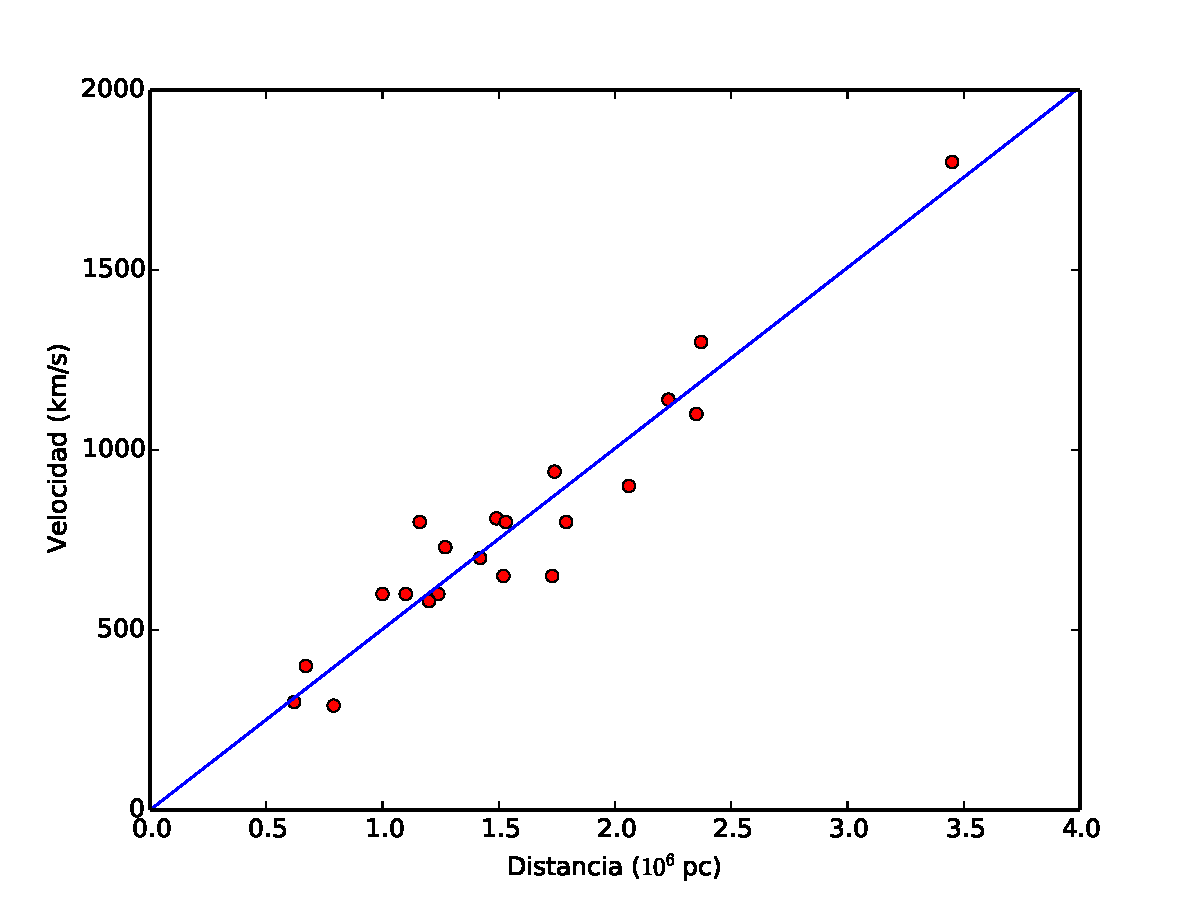
\includegraphics[width=0.7\textwidth]{fig/ajuste.pdf}
 \caption{Relaci'on entre la $velocidad$ y distancia de las nebulosas, medida por Hubble \cite{Hubble1}.}
  \label{hubble}
\end{figure}
Por otro lado, por comodidad es 'util definir el par'ametro adimensional $h$ tal que
\begin{equation}
H_0= 100 h \mbox{ km s}^{-1}\mbox{Mpc}^{-1} \label{h}
\end{equation}

%La figura (\ref{hubble}) muestra la recta originalmente ajustada por Hubble en 1929.
\section{Definiciones de Distancia}
Desde la aparici'on de la teor'ia de Relatividad Especial el concepto de distancia deja de ser una cantidad absoluta, por lo mismo 
se debe tener cuidado al momento de definir las distintas medidas de distancia usadas. En Cosmolog'ia la definici'on de distancia no es 'unica y se pueden 
emplear varios m'etodos para medirlas. Sus valores coinciden con la noci'on habitual de distancia para 
puntos cercanos ($r\ll 1$), pero difieren para puntos muy lejanos.\\
\subsection{Paralaje Trigonom'etrico}
El movimiento de la Tierra alrededor del Sol produce un movimiento aparente de la posici'on de alguna estrella alrededor
de una elipse. Para efectos pr'acticos se asume que la Tierra gira en una 'orbita circular cuyo radio es la distancia promedio
al Sol.
\begin{figure}[h]
  \centering
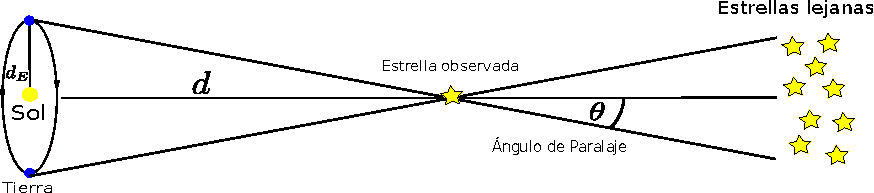
\includegraphics[width=0.8\textwidth]{fig/paralaje3.pdf}
 \caption{El movimiento de la Tierra alrededor del Sol.}
  \label{Paralaje}
  \end{figure}
Afortunadamente siempre la distancia de la Tierra a una estrella es mucho mayor que la distancia 
promedio de la Tierra al Sol (definida como \textit{Unidad Astron'omica}\footnote{$1\,AU= 1.496\times 10^{8}\,km$.} y simbolizada como $AU$) en ese caso el 'angulo de paralaje se puede aproximar
por la tangente entre ambos,
\begin{equation}
 \theta=\frac{d_{E}}{d},
\end{equation}
con $d_{E}$ la distancia Tierra-Sol y $d$ la distancia Tierra-Estrella.\\
A partir de esto podemos definir una nueva unidad de distancia, el \textit{P'arsec}\footnote{$1\,pc=206,264.8\,AU= 3.0856\times 10^{13}\,km = 3.2616\,\mbox{a\~nos luz}$.} (denotado con la sigla $pc$), como la distancia a la que 
debe estar un objeto para que el 'angulo de paralaje sea de $1"$. 
\subsection{Movimiento Propio}
Una fuente de luz a una distancia $d$ con  velocidad $v_{\bot}$ perpendicular a la l'inea de visi'on\footnote{L'inea recta imaginaria que une al observador con la estrella.}
parecer'a moverse a trav'es del cielo a una raz'on $\mu$ (en radianes/tiempo) dada por
\begin{equation}
\mu=\frac{v_{\bot}}{d}.
\end{equation}
Esto es conocido como movimiento propio. En general no se mide directamente esta cantidad, sino que la componente radial de la velocidad
$v_{\mbox{r}}$ a trav'es del efecto Doppler que genera el desplazamiento.\\ \\
'Ultimamente casi todas las mediciones de objetos dentro de nuestra galaxia se han efectuado usando alguno de estos dos m'etodos cl'asicos. Pero
si se desean medir la distancia a objetos mucho m'as lejanos dejan de ser adecuados, pues se basan en una visi'on cl'asica de un universo euclidiano.
\subsection{Luminosidad Aparente}
'Este es el m'etodo m'as usado para determinar distancias en Cosmolog'ia. Se basa en medir la potencia de luz emitida por un objeto,
cuya \textit{luminosidad absoluta} es conocida. La luminosidad absoluta $L$ se define como la potencia total radiada por el objeto 
(en todas direcciones). Entonces, asumiendo que la potencia radiada es la misma en todas direcciones podemos encontrar una simple 
relaci'on entre la potencia radiada total y la que recibir'ia un observador a una distancia $d$ del objeto.
\begin{equation}
l=\frac{L}{4\pi d^2}, \label{aparente}
\end{equation}
donde $l$ es la \textit{luminosidad aparente} recibida por el observador. Cabe se\~nalar que hemos considarado en esta 
expresi'on que el espacio es euclideano.
La expresi'on (\ref{aparente}) puede ser mejorada tomando en cuenta los efectos de la expansi'on del universo en la definici'on 
de $d$.\\ \\
Otro efecto importante a considerar es que un observador en la Tierra percibir'a una luminosidad aparente menor a la 
esperada por causa de la atm'osfera terrestre que absorbe parte de la luz recibida.
Se define la \textit{Magnitud Bolom'etrica} como la  magnitud aparente que tendr'ia una estrella si la radiaci'on
emitida por ella pudiera medirse en ausencia de la atm'osfera. Se representa por $M$ la magnitud absoluta y $m$ la aparente.\\
El astr'onomo brit'anico Norman Pogson en 1856 defini'o la escala moderna de magnitudes con base en la comparaci'on 
de luminosidades entre estrellas, de la cual se encuentra la relaci'on $l \propto 10^{2m/5}$. La constante 
de proporcionalidad pudo ser fijada en la d'ecada de 1930 con la llegada de las fotoceldas \cite{Hubble2}. 
De esta manera se obtuvo
\begin{equation}
l=10^{-2m/5}\times 2.52 \times 10^{-5} \left [\frac{erg}{cm^{2}s}\right ],
\end{equation}
 y la \textit{Magnitud bolom'etrica absoluta} $M$ 
\begin{equation}
L=10^{-2M/5}\times 3.02 \times 10^{35} \left [ \frac{erg}{s}\right ].
\end{equation}
Ambas expresiones son v'alidas para cualquier longitud de onda. Usando estas dos expresiones podemos reescribir (\ref{aparente}) como:
\begin{equation}
d=10^{1+(m-M)/5}pc.    \label{d}
\end{equation}
Hay muchos tipos de estrellas que son usadas para medir distancias a trav'es de la observaci'on de su luminosidad aparente.
\subsection{Velas Estandar}
'Estos son objetos estelares que pertenecen a una clase particular cuya luminosidad absoluta es conocida. Luego, por comparaci'on de luminosidades pueden ser
calculadas las distancias a otros objetos de la misma clase que se encuentren m'as lejanos a nuestra galaxia.
\paragraph{Cefeidas Variables:} Si se monitorea el brillo de ciertas estrellas, veremos que 'este oscila en el tiempo.
'Estas son conocidas como \textit{Estrellas variables}. El periodo de luminosidad puede variar desde minutos a meses o incluso
a\~nos. Dentro de este tipo de estrellas se encuentran las Cefeidas variables, cuyos periodos de luminosidad var'ian entre 1
a 100 d'ias y en nuestra galaxia se han encontrado  m'as de 1000.\\
Cuando se estudian las l'ineas espectrales en Cefeidas, se detectan corrimientos que var'ian con el mismo periodo que el de su 
luminosidad. Esto nos indica que la superficie de esta estrella se mueve, es decir, la luminosidad cambia como cambia la superficie
de la estrella.\\
Para entender esto consideremos una estrella com'un y corriente de radio $R_{0}$ y supongamos que 'esta es perturbada cambiando
su radio a $R$, tal que $R<R_{0}$, entonces debido a esta perturbaci'on su densidad y presi'on aumentar'an. El exceso en la presi'on
har'a que se expanda sobrepasando el radio de $equilibrio$ $R_{0}$. La disminuci'on en la presi'on generar'a que se vuelva
a comprimir, repiti'endose este proceso sucesivas veces.\\
En el an'alisis anterior dejamos de lado efectos importantes como la Opacidad\footnote{Un material presenta opacidad cuando no deja pasar luz en proporci'on apreciable.}.
En estrellas normales, la opacidad disminuye al aumentar la temperatura, esto significa, al comprimirse la estrella a causa del
aumento de presi'on tambi'en aumentar'a la temperatura y por lo tanto disminuir'a la opacidad. De este modo, cuando la estrella se expande
disminuye la presi'on y la temperatura, provocando un aumento en la opacidad. Esto genera los cambios peri'odicos en su luminosidad \cite{ceph2}.\\
En particular, las Cefeidas son un tipo de estrella variable con una gran luminosidad y por lo mismo son unas de las  m'as
usadas para medir distancias fuera de nuestra galaxia.
Adem'as, su periodo de luminosidad tiene una estrecha relaci'on con la misma luminosidad: entre mayor sea el periodo, mayor ser'a su luminosidad.
Calibrando la relaci'on entre luminosidad-periodo de Cefeidas cercanas se puede calcular la luminosidad de otras m'as lejanas
a trav'es de su periodo y por lo tanto nos permiten establecer distancias a trav'es de su luminosidad.
\begin{figure}[h!]
  \centering
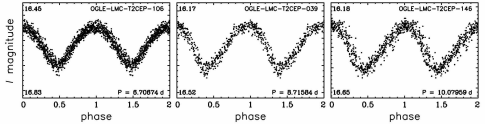
\includegraphics[width=0.8\textwidth]{fig/cepheid.png}
 \caption{Curvas de luz de tres Cefeidas ordinarias tipo II, con periodos similares \cite{ceph}.}
  %\label{}
  \end{figure}\\
\paragraph{Supernova Ia:} Se cree que ocurre cuando una enana blanca en un sistema binario aumenta su masa absorbiendo la de su
compa\~nera hasta acercarse al l'imite de Chandrasekhar\footnote{Es la m'axima masa posible de una estrella fr'ia estable. Si la estrella supera este l'imite  colapsa.}.
Cuando esto ocurre la enana blanca se vuelve inestable, aumentando su temperatura y densidad, generando explosiones
termonucleares las cuales pueden abarcar distancias de varios megaparsecs. Como todas estas estrellas explotan en condiciones
similares, la luminosidad de sus explosiones variar'an muy poco unas de otras, haciendo de las supernovas Ia un buen indicador de distancias.
\subsection{Distancia de Luminosidad}
Cuando se miden distancias con redshifts considerables ($z>0.1$) lo efectos de la expansi'on cosmol'ogica no pueden ser 
despreciados. Anteriormente encontramos una relaci'on entre la luminosidad absoluta y la luminosidad aparente (\ref{aparente})
a una distancia $d$, a la cual debemos hacer algunas correcciones.\\ \\
Imaginemos una estrella con coordenadas $\vec{x}_{1}=(ct_{1},r_{1},0,0)$ (en coordenadas esf'ericas), y que la tierra
se encuentra en las coordenadas $\vec{x}_{0}=(ct_{0},0,0,0)$, considerando (\ref{dsFRW}), la m'etrica inducida por una esfera centrada
(para un tiempo fijo) en $\vec{x}_{1}$ y que pasa por $\vec{x}_{0}$ ser'a 
\begin{equation}
 dl^2=a_{0}^2 r_{1}^2(d\theta^2  +\sen^2\theta d\varphi^2),\hspace{0.5cm} \mbox{con} \hspace{0.5cm}  a_{0}= a(t_{0}),
\end{equation}
cuya 'area es
\begin{equation}
A=4\pi a_{0}^2 r_{1}^2 . 
\end{equation}
Por otro lado, si la estrella emite $N$ fotones, de fecuencia $\nu_{1}$, en un intervalo de tiempo $\delta t_{1}$, la 
luminosidad absoluta ser'a:
\begin{equation} 
L=\frac{N h\nu_{1}}{\delta t_{1}}  \hspace{0.2cm} \Rightarrow \hspace{0.2cm} N=\frac{L\delta t_{1}}{h\nu_{1}},\label{Ltotal}
\end{equation}
con $h$ la constante de Planck. Un observador en $\vec{x}_{0}$ detectar'a $n$ fotones ($n<N$) en un 'area $S$ con frecuencia $\nu_{0}$, a causa del redshift,
en un intervalo de tiempo $\delta t_{0}$. Adem'as, al ser el espacio is'otropo cualquier observador que se encuentre en la superficie
esf'erica que encierra a la estrella recibir'a los mismos $n$ fotones con la misma frecuencia en el mismo intervalo de tiempo y superficie. As'i,
asumiendo que no hay p'erdida de fotones, por esta superficie esf'erica deber'an pasar en total $N$ fotones en el intervalo
de tiempo $\delta t_{0}$, es decir,
\begin{equation}
\int_{A}\frac{n}{S}dA=4\pi a_{0}^2 r_{1}^2 \frac{n}{S}= N.
\end{equation}
Entonces, podemos escribir la luminosidad aparente como
\begin{equation}
 l=\frac{nh\nu_{0}}{S\delta t_{0}} =\frac{Nh\nu_{0}}{4\pi a_{0}^2r_{1}^2\delta t_{0}}  \hspace{0.2cm} \Rightarrow \hspace{0.2cm} N=\frac{4\pi l a_{0}^2r_{1}^2\delta t_{0}}{h\nu_{0}},\label{laparente} 
\end{equation}
igualando (\ref{Ltotal}) y (\ref{laparente}) obtenemos
\begin{equation}
l=\frac{L}{4\pi a_{0}^2 r_{1}^2}\frac{\delta t_{1}}{\delta t_{0}}\frac{\nu_{0}}{\nu_{1}}.
\end{equation}
Adem'as, podemos relacionar $\delta t_{1}/\delta t_{0}$ y $\nu_{0}/\nu_{1}$ con el redshift cosmol'ogico usando (\ref{zc}) y (\ref{62i})
respectivamente. Con esto, encontramos la relaci'on
\begin{equation}
l =\frac{L}{4\pi a_{0}^2 r_{1}^2 (1+z)^2}.
\end{equation}
En base a este resultado, podemos definir la \textit{distancia de luminosidad} como
\begin{equation}
d_{L} :=  a_{0} r_{1} (1+z), \label{dl}
\end{equation}
tal que 
\begin{equation}
l=\frac{L}{4\pi d_{L}^2}.
\end{equation}
Por otro lado, usando (\ref{dl}) y (\ref{d}) podemos expresar la distancia de luminosidad en funci'on de las magnitudes absolutas y relativas de las estrellas.
\begin{equation}
m-M = 5\log\left(\frac{d_L(z)}{1pc}\right) - 5. \label{m-M}
\end{equation}
Esta definici'on de distancia resulta muy 'util para encontrar una relaci'on entre distancia y redshifts. Ahora la utilizaremos
en el caso particular en que $z\ll1$, para expandir en serie de potencias a segundo orden en $(t-t_{0})$:\\
\begin{eqnarray}
 a(t)&=&a(t_0)+\dot{a}(t_0)(t-t_0)+\frac{1}{2}\ddot{a}(t_0)(t-t_0)^2+\cdots \\
&=& a(t_0)\left[1+H_0(t-t_0)-\frac{1}{2}q_0H_0^2(t-t_0)^2+\cdots\right]. 
\end{eqnarray}
Aqu'i hemos definido el \textit{par'ametro de desaceleraci'on} $q_0$ como 
\begin{equation}
q_0:=-\frac{a(t_0)}{\dot{a}^2(t_0)}\ddot{a}(t_0).\label{q0}
\end{equation}
Luego,
\begin{equation}
\frac{a(t)}{a(t_0)}=1+H_0(t-t_0)-\frac{1}{2}q_0H_0^2(t-t_0)^2+\cdots .\label{z2}
\end{equation}
Pero $1+z=a(t_0)/a(t)$. Entonces, invirtiendo (\ref{z2}) encontramos
\begin{eqnarray}
 \frac{a(t_0)}{a(t)}&=&\left[1+H_0(t-t_0)-\frac{1}{2}q_0H_0^2(t-t_0)^2+\cdots\right]^{-1} \\
&=& 1+H_0(t_0-t)+\frac{1}{2}(q_0 +2)H_0^2(t_0-t)^2+ O\left[(t-t_{0})^3\right]\\
\Rightarrow z&\approx&H_0(t_0-t)+\frac{1}{2}(q_0 +2)H_0^2(t_0-t)^2.   \label{z3}
\end{eqnarray}
Esta expresi'on puede ser invertida\footnote{Basta con encontrar las raices de esta expresi'on y expandir a segundo orden en potencias de $z$.} expresando $t$ en funci'on de $z$
\begin{equation}
 H_{0}(t_0 -t)\approx  z -\frac{1}{2}(q_0 +2)z^2.
\end{equation}
Pero lo que deseamos hacer es relacionar la distancia de luminosidad con el redshift, para ello usaremos (\ref{60i}), que adopta la forma
\begin{equation}
\frac{c}{a(t_0)}\int_{t_1}^{t_0}\left[H_{0}t+\frac{1}{2}H_{0}^{2}(q_0 +2)t^2\right]dt \approx r_1.
\end{equation}
Como aproximamos a segundo orden en $(t-t_{0})$, podemos escribir
\begin{equation}
  \frac{r_1}{c} \approx \frac{t_0 -t_1}{a(t_0)} +\frac{H_{0}(t_0 -t_1)^2}{2a(t_0)}.\\
\end{equation}
\begin{equation}
   \frac{r_1}{c} a(t_0) H_0 \approx z -\frac{1}{2}(1+ q_0)z^2. \hspace{0.5cm}
\end{equation}
Manteniendo la aproximaci'on a segundo orden en $z$ y usando la definici'on de distancia de luminosidad (\ref{dl}) encontramos
\begin{equation}
d_{L}\approx \frac{c}{H_0}\left[z+\frac{1}{2}(1-q_0)z^2 \right]. \label{dlq0}
\end{equation}
Esta expresi'on tiene una buena precisi'on hasta redshifts de 0.2, para mayores valores la expansi'on en serie de potencias no es 'util.

\subsection{Distancia Angular}
Otra noci'on simple de distancia es la \textit{distancia angular}. Ella requiere conocer el tama\~no (lineal) ``real'' $D$
de un objeto (por ejemplo, una galaxia), entendido como su tama\~no medido por un observador que se mueve con el objeto. 
Si respecto a un observador lejano el objeto subtiende un 'angulo $\Delta\varphi$ entonces definimos la distancia angular
desde el observador al objeto como $d_A:=D/\Delta\varphi$.
\begin{figure}[h]
  \centering
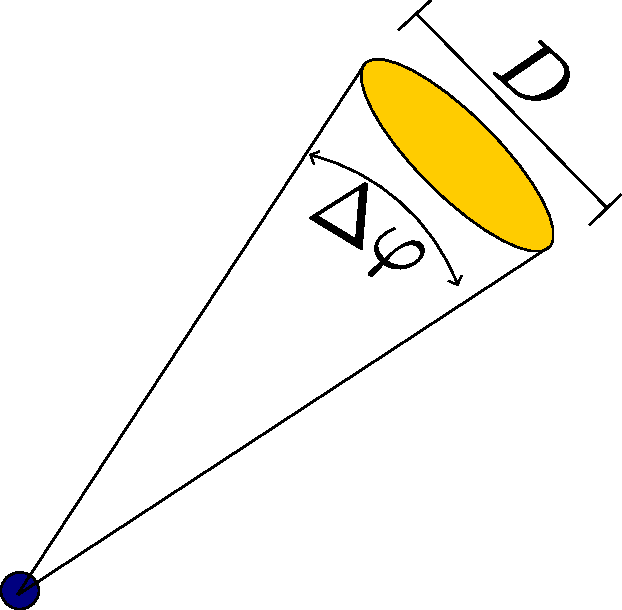
\includegraphics[width=0.3\textwidth]{fig/dangular.pdf}
 \caption{El punto azul representa la tierra mientras que el amarillo el objeto en estudio.}
 % \label{}
  \end{figure}\\
  Un c'alculo simple muestra que un objeto ubicado en la coordenada
$r_1$ en el tiempo $t_1$ tendr'a distancia angular dada por
\begin{equation}\marginnote{distancia angular}
 d_A=a(t_1)r_1.
\end{equation}

Es claro que tanto $d_L$ como $d_A$ coinciden con la definici'on usual de distancia si estamos en un 
universo plano sin expansi'on. Tambi'en es importante notar que para determinar tanto $d_A$ como $d_L$ es necesario 
conocer \textit{propiedades int'insecas} del objeto. Para calcular la distancia angular se requiere conocer el tama\~no
``real'' $D$ del objeto, mientras que para determinar la distancia de luminosidad se requiere la luminosidad absoluta $L$.

%\subsection{Relaci'on distancia de luminosidad - redshift}

%\begin{eqnarray}
% a(t)&=&a(t_0)+\dot{a}(t_0)(t-t_0)+\frac{1}{2}\ddot{a}(t_0)(t-t_0)^2+\cdots \\
%&=& a(t_0)\left[1+H_0(t-t_0)-\frac{1}{2}q_0H_0^2(t-t_0)^2+\cdots\right], \label{expR}
%\end{eqnarray}
%donde hemos definido la \textit{constante de Hubble} y el \textit{par'ametro de desaceleraci'on} por
%\begin{equation}
% H_0:=\frac{\dot{a}(t_0)}{a(t_0)},
%\end{equation}
%\begin{equation}
%q_0:=-\frac{a(t_0)}{\dot{a}^2(t_0)}\ddot{a}(t_0).
%\end{equation}
%Usando (\ref{expR}) podemos reescribir (\ref{zc}) como
%\begin{equation}
% z=H_0(t_0-t_1)+\left(1+\frac{q_0}{2}\right)H_0^2(t_0-t_1)^2+\cdots
%\end{equation}
%Invirtiendo esta expresi'on, encontramos
%\begin{equation}
% t_0-t_1=\frac{1}{H_0}\left[z-\left(1+\frac{q_0}{2}\right)z^2+\cdots\right].
%\end{equation}
%Con esto, podemos expresar la integral como
%\begin{equation}
% f(r_1)=\frac{c}{a(t_0)}\left[(t_0-t_1)+\frac{1}{2}H_0(t_0-t_1)^2+\cdots\right]
%\end{equation}
%\begin{equation}
% f(r_1)=\frac{c}{a(t_0)H_0}\left[z-\frac{1}{2}(1+q_0)z^2+\cdots\right]
%\end{equation}
%\begin{equation}
%d_L=\frac{c}{H_0}\left[z+\frac{1}{2}(1-q_0)z^2+\cdots\right]
%\end{equation}

\section{Ecuaciones de Einstein}

Como bien dijimos al principio del cap'itulo, a escalas cosmol'ogicas el universo (visto por observadores com'oviles con el fluido cosmol'ogico) luce homog'eneo e is'otropo. 
Esto implica que el tensor de energ'ia-mom'entum del fluido cosmol'ogico debe poseer estas mismas propiedades. Si suponemos que
el fluido cosmol'ogico es un fluido perfecto con presi'on $p$ y densidad de masa $\rho$, las componentes de su tensor energ'ia-mom'entum, debido a que la m'etrica
de espaciotiempo  es diagonal, ver (\ref{dsFRW}), ser'an
\begin{eqnarray}
T^{00}=\rho(t)c^2,\qquad T^{0i}=0, \qquad T^{ij}= -g^{ij}p(t),
\end{eqnarray}
donde $p$ y $\rho$ s'olo pueden depender del tiempo (por la isotrop'ia y homogeneidad). $T^{0i}=0$ tambi'en nos indica que el fluido cosmol'ogico
est'a en reposo respecto a observadores com'oviles con 'el ($u^\mu=(u^0,0,0,0)$).
De este modelo del universo podemos extraer informaci'on interesante. De la ec. de balance de la energ'ia %por ejemplo usando (\ref{dcT0})
\begin{eqnarray}
0 = \nabla_\mu T^{0\mu}&=& \frac{\partial T^{0\mu}}{\partial x^\mu} + \Gamma^{0}_{\mu\nu} T^{\nu \mu} + \Gamma^{\mu}_{\mu \nu} T^{0\nu}\\
                   &=& \frac{\partial T^{00}}{\partial x^0} + \Gamma^{0}_{ij} T^{ij} + \Gamma^{i}_{i0} T^{00},\\
\end{eqnarray}
obteniendo finalmente\footnote{Cabe mencionar que usando (\ref{a1}) y (\ref{a2}) tambi'en se puede obtener (\ref{rho}).}
\begin{equation}
\boxed{\dot \rho +3\frac{\dot a}{ac^2}(p+\rho c^2)= 0.} \label{rho} 
\end{equation}
Asumiendo la ecuaci'on de estado politr'opica
\begin{equation}
p=c^2\omega \rho,
\end{equation}
siendo $\omega$ independiente del tiempo, podemos encontrar una relaci'on entre $\rho$ y $a$ a partir de (\ref{rho}):
\begin{equation}
\rho =\rho_0 \left(\frac{a}{a_0}\right)^{-3(1+\omega)}.
\end{equation}
En el caso en que el fluido cosmol'ogico est'a compuesto mayoritariamente por materia no-relativista ($p\ll \rho c^{2}$), entonces $\omega \ll 1$ y por lo tanto
\begin{equation}
\rho =\rho_0 \left(\frac{a}{a_0}\right)^{-3}, \label{materia}
\end{equation}
o bien si fuese predominante la materia relativista ($p=c^{2}\rho/3$ , es decir $\omega = 1/3$)
\begin{equation}
\rho =\rho_0 \left(\frac{a}{a_0}\right)^{-4}. \label{radiacion}
\end{equation}
Por otro lado, de las ecuaciones de Einstein se puede obtener m'as informaci'on sobre la din'amica de la expansi'on del universo. De la componente $\mu=\nu=0$ de (\ref{EE3})
 y usando las conexiones calculadas anteriormente,
\begin{equation}
R_{00}=\frac{\partial\Gamma_{00}^\lambda}{\partial x^\lambda} -\frac{\partial\Gamma_{0\lambda}^\lambda}{\partial x^0}  +\Gamma^\lambda_{\lambda\rho}\Gamma^\rho_{00}  -\Gamma^\lambda_{0\rho}\Gamma^\rho_{0\lambda},          
\end{equation}
se obtiene
\begin{equation}
R_{00}=-\frac{3}{c^2}\frac{\ddot a}{a}.
\end{equation}
Adem'as,
\begin{equation}
T_{00}-\frac{1}{2}g_{00}T=\frac{4\pi G}{c^4}(\rho c^2+3p).
\end{equation}
Por lo tanto,
\begin{equation}
\boxed{\frac{3\ddot a}{a}=-\frac{4\pi G}{c^2}(\rho c^2+3p).} \label{a1}
\end{equation}
Por otro lado, sabemos que $T_{0i}=0$ y por los mismos motivos de homogeneidad del espacio $R_{0i}$ debe ser $0$. As'i, s'olo 
falta calcular $R_{ij}$,
\begin{equation}
R_{ij}=\frac{\partial\Gamma_{ij}^\lambda}{\partial x^\lambda} -\frac{\partial\Gamma_{j\lambda}^\lambda}{\partial x^i}  +\Gamma^\lambda_{\lambda\rho}\Gamma^\rho_{ij}  -\Gamma^\lambda_{i\rho}\Gamma^\rho_{j\lambda},   
\end{equation}
\begin{equation}
R_{ij}= \left[2k +\frac{2}{c^2}\dot a^2 +\frac{1}{c^2}a\ddot a\right] \mbox{\~g}_{ij},
\end{equation}
con $\mbox{\~g}_{ij}=\mbox{g}_{ij}/a^2$, adem'as
\begin{equation}
T_{ij}-\frac{1}{2}g_{ij}T=\frac{a^2}{2c^2}(\rho c^2- p)\mbox{\~g}_{ij}.
\end{equation}
Por lo tanto,
\begin{equation}
\boxed{\frac{2kc^2}{a^2} +\frac{2\dot a^2}{a^2} +\frac{\ddot a}{a}= \frac{4\pi G}{c^2}(\rho c^2- p).} \label{a2}
\end{equation}
Usando (\ref{a1}) y (\ref{a2}) se pueden eliminar las segundas derivadas, obteniendo
\begin{equation}
\boxed{\dot a^2 +kc^2  = \frac{8\pi G\rho a^2}{3}.} \label{dota}
\end{equation}
'Esta es la ecuaci'on fundamental de Friedmann \cite{friedmann} que gobierna la expansi'on del universo.\\
De aqu'i vemos que la expansi'on s'olo puede detenerse en un universo con curvatura positiva, es decir $k=1$.\\
En base a (\ref{dota}) podemos definir la \textit{densidad de masa cr'itica} actual como
\begin{equation}
\rho_{0\rm{,crit}}:= \frac{3H_0^2}{8\pi G} = 1.878\times 10^{-29} h^2 \mbox{ g/cm}^3,
\end{equation}
donde $h$ es la constante de Hubble en unidades de $100$ km s$^{-1}$Mpc$^{-1}$. Es llamada as'i pues despejando $\rho$ de
(\ref{dota}) se obtiene
\begin{equation}
\rho = \frac{3\dot a^2}{8\pi Ga^2} + \frac{3kc^2}{8\pi Ga^2}, \label{densidad}
\end{equation}
lo que significa que
\begin{equation}
\rho_0 = \frac{3 H_0^2}{8\pi G} + \frac{3kc^2}{8\pi Ga_0^2} = \rho_{0\rm{,crit}} + \frac{3kc^2}{8\pi Ga_0^2}. 
\end{equation}
Si $\rho_0 > \rho_{0\rm{,crit}}$ estamos en un universo con curvatura espacial positiva.
Si $\rho_0=\rho_{0\rm{,crit}}$ estamos en un universo espacialmente plano. Si $\rho_0<\rho_{0\rm{,crit}}$ estamos en un universo curvatura espacial negativa.
Es decir, $\rho_{0\rm{,crit}}$ es un \textit{punto de inflecci'on} para el valor de la densidad, entre estos tres posibles casos.\\
De la definici'on (\ref{q0}) y la ec. (\ref{a1}) encontramos la expresi'on
\begin{equation}
q_{0}=\frac{4\pi G}{3c^2 H_0^2}(\rho_0 c^2 +3p_0)=\frac{\rho_0 c^2 +3p_0}{2\rho_{0\rm{,crit}}} . \label{q00}
\end{equation}

Por otro lado, analizando (\ref{a1}) vemos que este modelo s'olo permite una expansi'on desacelerada, ya que, si $c^2\rho+ 3p$ proviene de una mezcla de
radiaci'on y materia $q_0>0$ y $\ddot a<0$. Esto tiene mucho sentido, pues en ausencia de cualquier otro tipo de fuerzas, la
atracci'on gravitacional ser'a la 'unica que domine el comportamiento del universo a escalas cosmol'ogicas.\\
Otra de las consecuencias de este modelo es que la edad actual del 
universo es mayor que el tiempo de Hubble. Si graficamos  $a(t)/a_0$ vs $t$ entonces $H_0$ es la pendiente de la curva en $t_0$,
por lo tanto cualquier modelo del universo debe tener dicha pendiente en $t_0$.\\
\begin{figure}[h!]
  \centering
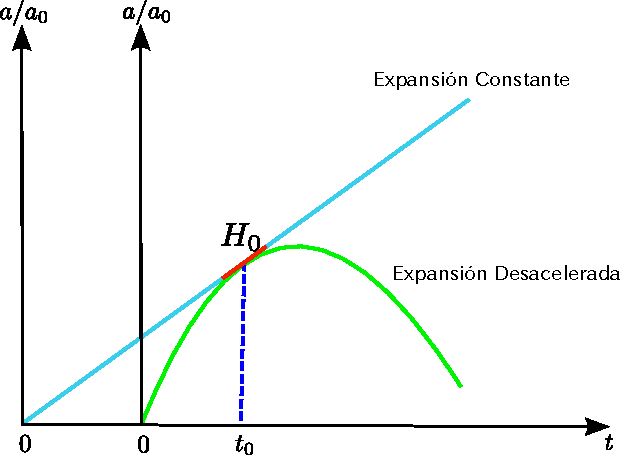
\includegraphics[width=0.55\textwidth]{fig/ex.pdf}
 \caption{Como se puede observar del gr'afico, si la expansi'on es desacelerada el tiempo transcurrido desde $a=0$ hasta $a_0$ es menor que el de un modelo de expansi'on a velocidad constante.}
 % \label{}
  \end{figure}\\
Como ya hemos visto, actualmente se sabe que la expansi'on del universo no es desacelerada,
por el contrario, el universo se expande en forma acelerada, por lo que el modelo propuesto no se ajusta a las observaciones.
Esto puede ser solucionado agregando la Constante Cosmol'ogica $\Lambda$ a las ecuaciones de Einstein\footnote{Ver ecuaci'on (\ref{EE2}).}
tal que $\ddot a > 0$. Esta constante tiene dos interpretaciones distintas. 
La primera, es que 'esta es una correcci'on a las ecuaciones de Einstein, la que s'olo es significativa a escalas cosmol'ogicas. 
La segunda, requiere poner esta constante al otro lado de la igualdad,
\begin{equation}
R_{\mu \nu} -\frac{1}{2}Rg_{\mu \nu} = \frac{8\pi G}{c^4}T_{\mu \nu}+ \Lambda g_{\mu \nu} = \frac{8\pi G}{c^4}T^{\prime}_{\mu \nu}, \label{TEL}
\end{equation}
as'i $T^{\prime}_{\mu \nu}$ corresponde al tensor energ'ia-momentum de la materia que conforma el universo conocido m'as 
otro tipo de \textquotedblleft materia\textquotedblright  con densidad de masa y presi'on tales que $\ddot a > 0$.\\
En ese caso, el tensor de energ'ia-momentum de este fluido desconocido ser'ia
\begin{equation}
T^{\Lambda}_{\mu\nu}=\frac{c^4\Lambda}{8\pi G} g_{\mu\nu}.
\end{equation}
Puede identificarse este energ'ia-momentum como el de un fluido perfecto con densidad y presi'on dadas por,
\begin{eqnarray}
\rho_{\Lambda}=\frac{c^2\Lambda}{8\pi G},    \qquad
p_{\Lambda}=-\frac{c^4\Lambda}{8\pi G}.
\end{eqnarray}
Por lo que este supuesto fluido satisface una ec. de estado politr'opica,
\begin{equation}
p=-\rho c^2,
\end{equation}
es decir, aqu'i  $\omega=-1$.\\
Entonces, si aparte del fluido cosmol'ogico agregamos este nuevo fluido a (\ref{a1}), obtenemos
\begin{equation}
\frac{3\ddot a}{a}=-\frac{4\pi G}{c^2}(\rho c^2+3p)+\Lambda c^2. 
\end{equation}
Entonces, para que $\ddot a$ sea mayor a cero $\Lambda$ debe satisfacer
\begin{equation}
\Lambda > \frac{4\pi G}{c^4}(\rho c^2 + 3p),
\end{equation}
Esto significa que $\Lambda$ debe ser una constante positiva, y por consiguiente genera presi'on efectiva negativa, tal que
contrarresta la atracci'on gravitacional.\\ \\
Ahora bien, supongamos que el universo est'a conformado por materia relativista y materia no-relativista las cuales no interactuan en forma significativa entre ellas  y adem'as agregamos la constante cosmol'ogica, entonces

\begin{equation}
\rho = \rho_{\rm{R}} + \rho_{\rm{M}} + \rho_{\rm{\Lambda}},
\end{equation}
aqu'i $\rho_{\rm{R}}$ representa la densidad de masa de la materia relativista, $\rho_{\rm{M}}$ la densidad de masa de la materia no relativista y $\rho_\Lambda$ representa una densidad de masa efectiva a causa de la constante cosmol'ogica. Reemplazando con (\ref{materia}) y (\ref{radiacion}), encontramos
\begin{equation}
\rho = \rho_{0\,\rm{R}}\left(\frac{a_0}{a}\right)^{4} + \rho_{0\,\rm{M}}\left(\frac{a_0}{a}\right)^{3} + \rho_{\rm{\Lambda}}.
\end{equation}
Podemos reescribir la densidad de masa como:
\begin{equation}
\rho = \frac{3H_0^2}{8\pi G}\left[\Omega_{\rm{R}}\left(\frac{a_0}{a}\right)^{4} + \Omega_{\rm{M}}\left(\frac{a_0}{a}\right)^{3} + \Omega_{\rm{\Lambda}}\right], \label{ro0}
\end{equation}
con
\begin{eqnarray}
\Omega_{\rm{R}} := \frac{3H_0^2\rho_{0\,\rm{R}}}{8\pi G},\qquad 
\Omega_{\rm{M}} := \frac{3H_0^2\rho_{0\,\rm{M}}}{8\pi G}, \qquad
\Omega_{\rm{\Lambda}} := \frac{3H_0^2 \rho_{0\,\rm{\Lambda}}}{8\pi G},
\end{eqnarray}
tal que al evaluar (\ref{dota}) en $t_0$ obtenemos
\begin{equation}
\hspace{2cm} \Omega_{\rm{R}} +\Omega_{\rm{M}} +\Omega_{\rm{\Lambda}} +\Omega_{\rm{k}} =1, \hspace{1cm} \mbox{con} \hspace{0.2cm} \Omega_{\rm{k}} := -\frac{kc^2}{a_0^2H_0^2}. 
\end{equation}
Adem'as, podemos escribir la presi'on actual como
\begin{equation}
p_0=\frac{3H_0^2}{8\pi G}\left( -\Omega_{\rm{\Lambda}}  +\frac{1}{3}\Omega_{\rm{R}} \right). \label{p0}
\end{equation}
Reemplazando (\ref{p0}) y (\ref{ro0}) en (\ref{q00}), se obtiene que
\begin{equation}
q_0=\frac{1}{2}(\Omega_{\rm{M}} + 2\Omega_{\rm{R}}  - 2\Omega_{\rm{\Lambda}}).  \label{q0omega}
\end{equation}
Por otro lado, usando (\ref{dota}) vemos que
\begin{equation}
 \dot a^2 = H_0^2 a^2\left[\Omega_{\rm{R}}\left(\frac{a_0}{a}\right)^{4} + \Omega_{\rm{M}}\left(\frac{a_0}{a}\right)^{3} + \Omega_{\rm{\Lambda}} +\Omega_{\rm{k}}\left(\frac{a_0}{a}\right)^{2} \right]. 
\end{equation}
Luego, definiendo $x=:a/a_0$, podemos escribir 
\begin{equation}
\dot x^2 =H_0^2 x \left[\Omega_{\rm{R}}x^{-4} + \Omega_{\rm{M}}x^{-3}  +\Omega_{\rm{k}}x^{-2} + \Omega_{\rm{\Lambda}}\right].
\end{equation}
Usando (\ref{zc}) y despejando $t$ en funci'on de $z$, obtenemos
\begin{equation}
t(z)=\frac{1}{H_0}\int_0^{1/(1+z)}\frac{dx}{x\sqrt{\Omega_{\rm{R}}x^{-4} + \Omega_{\rm{M}}x^{-3}+\Omega_{\rm{k}}x^{-2} + \Omega_{\rm{\Lambda}} }}.
\end{equation}
Esta expresi'on nos permite calcular la edad actual del universo como
\begin{equation}
t_0=\frac{1}{H_0}\int_0^1\frac{dx}{x\sqrt{\Omega_{\rm{R}}x^{-4} + \Omega_{\rm{M}}x^{-3}+\Omega_{\rm{k}}x^{-2} + \Omega_{\rm{\Lambda}} }}. \label{tiempo}
\end{equation}
Por otro lado, de (\ref{60i}) vemos que
\begin{equation}
f(r(z))=c\int_{t_0}^{t(z)}\frac{dt}{a(t)}= \frac{c}{a_0H_0}\int_{1/(1+z)}^1\frac{dx}{x^2\sqrt{\Omega_{\rm{R}}x^{-4} + \Omega_{\rm{M}}x^{-3}+\Omega_{\rm{k}}x^{-2} + \Omega_{\rm{\Lambda}} }}.
\end{equation}
Luego,
\begin{equation}
r(z)=S\left[\frac{c}{a_0H_0}\int_{1/(1+z)}^1\frac{dx}{x^2\sqrt{\Omega_{\rm{R}}x^{-4} + \Omega_{\rm{M}}x^{-3}+\Omega_{\rm{k}}x^{-2} + \Omega_{\rm{\Lambda}} }}\right],
\end{equation}
con
\begin{equation}
S\left[y\right]=\left\{
\begin{array}
[c]{ccl}%
\text{sen}(y), &\text{si}& k=+1\\
y, &\text{si}& k=0\\
\text{senh}(y), &\text{si}& k=-1
\end{array}
\right. . \label{61i2}%
\end{equation}
Entonces, usando la definici'on de distancia de luminosidad (\ref{dl}), encontramos
\begin{equation}
d_L(z)=a_0(1+z)S\left[\frac{c}{a_0H_0}\int_{1/(1+z)}^1\frac{dx}{x^2\sqrt{\Omega_{\rm{R}}x^{-4} + \Omega_{\rm{M}}x^{-3} +\Omega_{\rm{k}}x^{-2} + \Omega_{\rm{\Lambda}}}}\right]. \label{dlzk}
\end{equation}
En particular para el caso $k=0$ tenemos que $\Omega_k=0$ y por lo tanto
\begin{equation}
\boxed{d_L(z)=\frac{(1+z)c}{H_0}\int_{1/(1+z)}^1\frac{dx}{x^2\sqrt{\Omega_{\rm{R}}x^{-4} + \Omega_{\rm{M}}x^{-3} + \Omega_{\rm{\Lambda}}}}.} \label{dlz}
\end{equation}



%\begin{align}
%G_{00} &= \frac{3}{c^2}\left(\frac{\dot{a}^2}{a^2}+\frac{kc^2}{a^2}\right), \\
%G_{rr} &=-\frac{1}{c^2(1-kr^2)}\left(2R\ddot{a}+\dot{a}^2+kc^2\right) = \frac{g_{rr}}{c^2}\left(2a\ddot{a}+\dot{a}^2+kc^2\right), \\
%G_{\theta\theta} &= -\frac{r^2}{c^2}\left(2a\ddot{a}+\dot{a}^2+kc^2\right) 
%=\frac{g_{\theta\theta}}{c^2}\left(2a\ddot{a}+\dot{a}^2+kc^2\right) , \\
%G_{\varphi\varphi} &= G_{\theta\theta}\sen^2\theta
%=\frac{g_{\varphi\varphi}}{c^2}\left(2a\ddot{R}+\dot{a}^2+kc^2\right).
%\end{align}

%\begin{align}
%T_{00} &= \rho c^2, \\
%T_{rr} &= -p\, g_{rr}, \\
%T_{\theta\theta} &= -p\, g_{\theta\theta}, \\
%T_{\varphi\varphi} &= -p\, g_{\varphi\varphi}.
%\end{align}
\section{Datos experimentales, Modelos y Ajustes}
         
Como hemos visto, este modelo cosmol'ogico nos permite obtener mucha informaci'on sobre el universo, sobre su curvatura, su edad y tipo de 
materia que lo compone. Entonces es momento de poner a prueba nuestros modelos del universo, usando los datos experimentales.\\ \\
El Proyecto Cosmol'ogico de Supernovas (Supernova Cosmology Project\footnote{Sitio web: \url{http://supernova.lbl.gov/}.} o abreviado por sus siglas SCP) es uno de los dos equipos de investigaci'on que determinaron
que el universo se expande en forma acelerada. Ellos usaron cientos de datos tomados del redshift de supernovas tipo Ia.
El SCP Union2.1 SN Ia\footnote{Direcci'on web: \url{http://supernova.lbl.gov/Union/}.} es una compilaci'on de datos obtenidos de las supernovas Ia.
Como se puede ver en el link al pie de la p'agina, estos datos est'an en una tabla donde la primera columna corresponde al nombre de la
supernova, la segunda al redshift medido, la tercera columna corresponde a la cantidad $m-M$ y la cuarta columna corresponde al error asociado a la medici'on de $m-M$.
\begin{equation}
\begin{array}{lccl}
\mbox{Nombre} & z        &     m-M       & \mbox{Error } m-M\\
1993\mbox{ah} & 0.028488 & 35.3465833928 & 0.223905932998	\\
1993\mbox{ag} & 0.050043 & 36.6823679154 & 0.166828851413	\\
1993\mbox{o}  & 0.052926 & 36.8176912545 & 0.1557559148	\\
1993\mbox{b}  & 0.070086 & 37.4467365424 & 0.158466934433	\\
1992\mbox{bs} & 0.062668 & 37.4834093505 & 0.156099434739	\\
...    & ...	  & ...	      	  & ...
\end{array}
\end{equation}
Estos mismos datos ser'an los que utilizaremos
para ajustar los par'ametros de nuestro modelo. Los gr'aficos de la figura \ref{zvsm-M}, corresponden a los datos obtenidos 
de las supernovas tipo Ia por el SCP.
\begin{figure}[h!]
  \centering
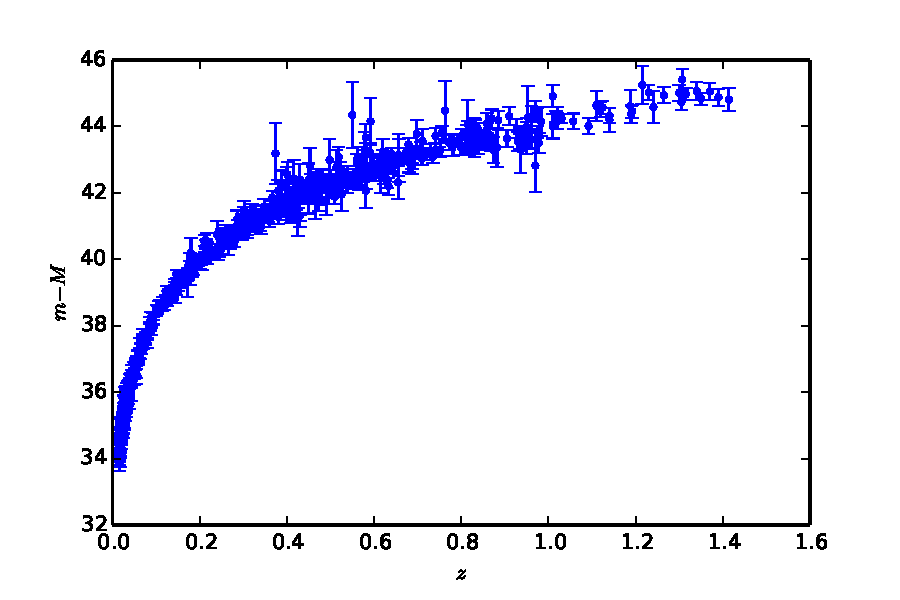
\includegraphics[width=0.48\textwidth]{fig/m-M-versus-z-con-error.pdf}
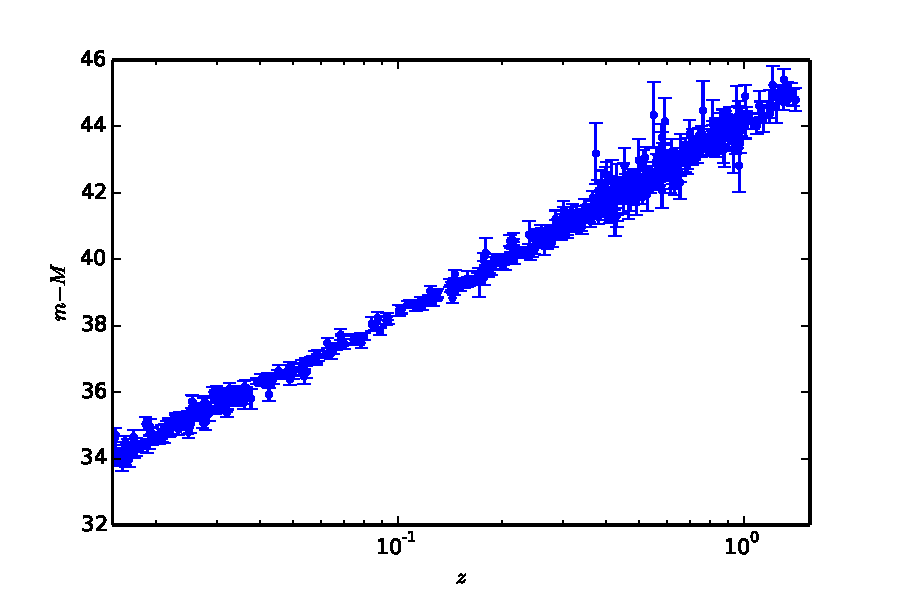
\includegraphics[width=0.48\textwidth]{fig/m-M_vs_z_semilog.pdf}
 \caption{El gr'afico superior corresponde a m-M versus redshift, mientras que el inferior es una representaci'on semilogar'itmica procedentes de supernovas tipo Ia. Ambos con barras de error.}
  \label{zvsm-M}
  \end{figure}\\
Ahora bien, de (\ref{m-M}) y (\ref{dlq0}) y usando el m'etodo de m'inimos cuadrados ponderados podemos en contrar los valores de 
$h$ y $q_0$ que se ajustan mejor a los datos (en el apendice se encuentra una secci'on con los scripts utilizados). Dichos valores
resultan ser
\begin{eqnarray}
h=0.688 \qquad; \hspace{0.5cm} q_0=-0.175\hspace{0.1cm}. 
\end{eqnarray}
Esto significa que el universo debe estar en expansi'on acelerada pues $q_0<0$. Adem'as con el valor de $h$  obtenido 
y (\ref{h}), tenemos que $H_0= 68,8 \mbox{ km s}^{-1}\mbox{Mpc}^{-1}$. Se debe mencionar tambi'en, que el valor de $q_0$
no es muy preciso, pues como se ve en los datos, hay redshifts de hasta $1.4$ lo que es bastante grande para la aproximaci'on 
a segundo orden en $z$.\\
\begin{figure}[h!]
  \centering
\includegraphics[width=0.7\textwidth]{fig/datos-y-ajusteq0.pdf}
 \caption{Gr'afico correspondiente al ajuste de la expresi'on a segundo orden en $z$. Con $h=0.688$ y $q_0=-0.175$.}
  \label{q000}
  \end{figure}\\
De la figura (\ref{q000}), se ve que la curva se ajusta muy bien a los datos observacionales, pero es conveniente hacer
un estudio un poco m'as profundo para dilucidar si este ajuste  es bueno. Con este propocito utilizaremos el diagrama de residuos
y su correspondiente histograma. C'omo se puede apreciar de (\ref{res}), el diagrama de residuos nuestra una distribuci'on 
m'as o menos aleatoria en torno a cero, esto significa que el ajuste pasa aproximadamente por en medio de todos los puntos. Esto
es corroborado por su histograma, ya que presenta aproximadamente una forma de distribuci'on normal\footnote{El Teorema del l'imite central establece que, bajo ciertas condiciones, la suma de un gran n'umero de variables aleatorias se aproxima a una distribuci'on normal.}. 
\begin{figure}[h!]
  \centering
\includegraphics[width=0.48\textwidth]{fig/residuosnorq0.pdf}
\includegraphics[width=0.48\textwidth]{fig/gaussq0.pdf}
 \caption{El gr'afico de la izquierda corresponde al diagrama de residuos del ajuste, mientras que el de la derecha corresponde 
 al histograma de residuos al cual se le ajust'o una curva gaussiana, con $\sigma^2$ la varianza y $\mu$ la media.}
  \label{res}
  \end{figure}\\ \\      
Este mismo an'alisis se puede hacer con los modelos definidos por la relaci'on (\ref{dlzk}), usando m'inimos cuadrados ponderados podemos ajustar 
los par'ametros de los 3 modelos ($k=-1,0,1$). En la figura \ref{datosyajustes} vemos los 3 modelos. Es dif'icil discernir entre cu'al de los tres
es el mejor, ya que en los 3 casos las curvas se ajustan muy bien a los datos y adem'as los valores de los par'ametros obtenidos son muy similares. Para el caso $k=-1$ se tiene
\begin{eqnarray}
h=0.7001,\quad\Omega_\Lambda=0.7237,\quad\Omega_M=0.2731,\quad\Omega_R=0.0024,\quad\Omega_k=0.0008.\hspace{0.1cm} 
\end{eqnarray}
Para el caso $k=0$,
\begin{eqnarray}
h=0.7000,\quad\Omega_\Lambda=0.7225,\quad\Omega_M=0.2773,\quad\Omega_R=0.0002,\quad\Omega_k\equiv0\hspace{1.1cm}
\end{eqnarray}
Para el caso $k=1$,
\begin{eqnarray}
h=0.7000,\quad\Omega_\Lambda=0.7231,\quad\Omega_M=0.2765,\quad\Omega_R=0.0005,\quad\Omega_k=-0.0001.
\end{eqnarray}
\begin{figure}[h!]
  \centering
\includegraphics[width=0.49\textwidth]{fig/datos-y-ajustek-1.pdf}
\includegraphics[width=0.49\textwidth]{fig/datos-y-ajustek1.pdf}
\includegraphics[width=0.60\textwidth]{fig/datos-y-ajuste.pdf}
 \caption{El gr'afico superior izquierdo corresponde al caso de un universo con curvatura espacial negativa, el superior
 derecho al caso de un universo con curvatura espacial positiva y el inferior central, al caso de un universo espacialmente plano.}
  \label{datosyajustes}
\end{figure}\\
\begin{figure}[h!]
  \centering
\includegraphics[width=0.49\textwidth]{fig/residuosnork-1.pdf}
\includegraphics[width=0.49\textwidth]{fig/residuosnork1.pdf}
\includegraphics[width=0.55\textwidth]{fig/residuosnor.pdf}
\includegraphics[width=0.49\textwidth]{fig/gaussk-1.pdf}
\includegraphics[width=0.49\textwidth]{fig/gaussk1.pdf}
\includegraphics[width=0.55\textwidth]{fig/gaussk0.pdf}
 \caption{Diagrama de residuos correspondientes a los tres distintos valores de $k$, con sus respectivos histogramas.}
  \label{residuos}
\end{figure}\\
En los tres casos los par'ametros toman valores similares, alrededor del $73\%$ de la densidad de masa del universo es contribuida
por la constante cosmol'ogica y el $27\%$ restante es contribuido por la materia no-relativista. Por otro lado, la contribuci'on
de la materia relativista no alcanza el $1\%$. Adem'as, reemplazando en (\ref{tiempo}) los valores obtenidos, podemos
calcular las correspondientes edades del universo, que nuevamente resultan muy similares para los 3 casos.\\
\begin{equation}
\begin{array}{ll}
k=-1,& \mbox{Edad del Universo} \approx 13.66 \mbox{ miles de Millones de a\~nos}.\\
k=0, & \mbox{Edad del Universo} \approx 13.75 \mbox{ miles de Millones de a\~nos}.\\
k=1, & \mbox{Edad del Universo} \approx 13.73 \mbox{ miles de Millones de a\~nos}.\\
\end{array}
\end{equation}
As'i mismo, sus respectivos diagramas de residuos e histogramas, como vemos en la figura \ref{residuos}, presentan formas muy similares.
Por otro lado, con estos valores obtenidos y de (\ref{q0omega}) podemos obtener valores m'as precisos de $q_0$, ya que el obtenido anteriormente
proviene de una aproximaci'on a segundo orden en $z$. Para $k=-1$ se tiene que $q_0=-0.5848$, mientras que para $k=0$ se obtiene $q_0=-0.5836$, por 'ultimo,
 en el caso $k=1$ el valor obtenido es $ q_0=-0.5844$. Estos tres valores de $q_0$ son aproximadamente tres veces m'as grandes que el anteriormente
 calculado.\\
 
 Por otro lado, podemos calcular el \textit{Coeficiente de determinaci'on} de nuestros ajustes, definido como 
\begin{equation}
 R^2:=1- \frac{\sum_i(y_i-f_i)^2}{\sum_i(y_i- \bar{y})^2},
\end{equation}
con $y_i$ los datos utilizados, $f_i$ el ajuste usado y $\bar{y}$ el promedio de todos los datos. Entre m'as cercano sea $R^2$ a uno
mejor es el ajuste, por el contrario, si $R^2$ se aproxima a cero entonces el ajuste no es muy confiable.\\
Los coeficientes de determinaci'on obtenidos fueron:
\begin{equation}
\begin{array}{rl}
\mbox{Aproximaci'on a segundo orden en $z$:}& R^2 = 0.992795,\\
\mbox{Modelo con $k=-1$:}& R^2 = 0.993036,\\
\mbox{Modelo con $k=0$:} & R^2 = 0.993036, \\
\mbox{Modelo con $k=1$:} & R^2 = 0.993036.
\end{array}
\end{equation}
Como es de esperarse, la aproximaci'on a segundo orden en $z$, no es tan buena como los ajustes de los tres modelos, pues es s'olo una 
aproximaci'on. Por otro lado, el coeficiente de determinaci'on no nos permite distinguir qu'e modelo del universo es mejor ($k=-1,0,1$).\\
 
 
Pero a'un no hemos corroborado la importancia de la constante cosmol'ogica. Ya que todos los modelos son muy parecidos, consideraremos $k=0$ por su simplicidad. 
En la figura \ref{parametros}, hemos graficado nuestro modelo con valores de $\Omega_\Lambda$, $\Omega_R$ y $\Omega_M$ asignados por nosotros. Para las tres curvas
elegimos $h=0.7$.
\begin{figure}[h!]
  \centering
\includegraphics[width=0.49\textwidth]{fig/parametros_de_prueba.pdf}
\includegraphics[width=0.49\textwidth]{fig/zoom.pdf}
 \caption{El gr'afico de la izquierda corresponde a las curvas del modelo con $k=0$, para algunos valores de los par'ametros asignados por nosotros. 
 El gr'afico de la derecha corresponde a un zoom de la parte superior del gr'afico de la izquierda. Las tres curvas para redshifts peque\~nos se ajustan bien los datos, pero para redshifts mayores toma mayor importancia el
 tipo de materia presente en el universo.}
  \label{parametros}
\end{figure}\\
En el caso l'imite de un universo vac'io, s'olo con constante cosm'olgica (la curva de color rojo), el modelo predice una expansi'on mayor a la observada. Por otro lado, en un universo
s'olo con materia relativista y no-relativista (curva de color negro), predice una expansi'on menor a la observada. En sus respectivos diagramas de residuos se
ve que hay tendencias que se dejan fuera para estos dos casos.\\
%Recordemos que introdujimos las constante cosmol'ogica para poder describir la expansi'on acelerada del universo, en su aucencia
\begin{figure}[h!]
  \centering
\includegraphics[width=0.49\textwidth]{fig/resparametros1.pdf}
\includegraphics[width=0.49\textwidth]{fig/resparametros3.pdf}
 %\caption{}
  \label{parametros2}
\end{figure}\\
Adem'as, podemos elegir de antemano $\Omega_\Lambda=0$ y usar el m'etodo de m'inimos cuadrados para ajustar (\ref{dlzk}) a los datos.  
\begin{figure}[h!]
  \centering
\includegraphics[width=0.70\textwidth]{fig/datos-y-ajustelambda0.pdf}
 %\caption{}
  \label{lambda0}
\end{figure}\\     
La curva se ajusta muy bien a los datos, y parece no ser necesaria la constante cosmol'ogica, pero el valor obtenido de los par'ametros ajustados son:
$h= 0.6645$, $\Omega_M=1.7057$ y $\Omega_R=-0.7057$. Es claro que esto se aleja de la realidad f'isica del problema, pues $\rho_R>0$.
Por lo que, la constante cosmol'ogica es necesaria en este modelo del universo.

Por otro lado, podemos hacer un an'alisis estad'istico de nuestros ajustes, con los contornos de confianza (confidence contours) de los
par'ametros ajustados. Esto es un intervalo de n'umeros entre los cuales se estima que estar'a cierto valor
desconocido con una determinada probabilidad de acierto. Esta probabilidad se calcula a partir de datos de una muestra, y los valores desconocidos
son los par'ametros a ajustar. La probabilidad de 'exito en la estimaci'on se representa con $1-\alpha$ y se denomina nivel de confianza. Aqu'i $\alpha$ 
es el llamado error aleatorio o nivel de significaci'on y es una medida de las posibilidades de fallar en la estimaci'on mediante tal intervalo.
El nivel de confianza y la amplitud del intervalo var'ian conjuntamente, de forma que un intervalo m'as amplio tendr'a m'as probabilidad
de acierto (mayor nivel de confianza). Mientras que, para un intervalo m'as peque\~no, la estimaci'on es m'as precisa, pero aumenta su
probabilidad de error. Es habitual que el par'ametro presente una distribuci'on normal.

Los valores m'inimos de $\chi^2$ en los cuatro casos son:


\begin{eqnarray}
\mbox{Aprox. a segundo orden en $z$}: \qquad \chi^2\approx581.39,\\
\mbox{Expresi'on completa, caso $k=-1$}: \qquad \chi^2\approx 562.23,\\
\mbox{Expresi'on completa, caso $k=0$}:  \qquad \chi^2\approx 562.23,\\
\mbox{Expresi'on completa, caso $k=1$}:  \qquad \chi^2\approx 562.23.
\end{eqnarray}
\begin{figure}[h]
  \centering
\includegraphics[width=0.65\textwidth]{fig/contornoq0.pdf}
\includegraphics[width=0.65\textwidth]{fig/contornok-1.pdf}
\includegraphics[width=0.65\textwidth]{fig/contornok0.pdf}
\includegraphics[width=0.65\textwidth]{fig/contornok1.pdf}
 \caption{Contornos de confianza de nuestros modelos. La barra lateral indica el valor de $\chi^2$ dependiendo del valor de los par'ametros. Los
 valores de $h$ y $\Omega_k$ utilizados son los obtenidos por m'inimos cuadrados en cada caso. La x el punto en que $\chi^2$ alcanza su valor m'inimo.}
  \label{parametros22}
\end{figure}

Por otro lado, como la estad'istica de $\chi^2$ es una variable aleatoria, se le puede asignar una distribuci'on de probabilidad, dada por
\begin{eqnarray}
X(\chi^2;\nu)= \frac{(\chi^2)^{(\frac{\nu}{2}-1)}\exp[-\chi^2/2]}{2^{\nu/2}\Gamma(\nu/2)}, \qquad \mbox{con} \qquad \nu=\mbox{N}-\mbox{\textit{N}}.
\end{eqnarray}
Donde $\nu$ son los grados de libertad del ajuste, es decir, es el n'umero de datos usados menos el n'umero de par'ametros a ajustar. En la
figura \ref{parametros3} se muestra el gr'afico correspondientes a la densidad de probabilidad de $\chi^2$.\\ 
\begin{figure}[h!]
  \centering
\includegraphics[width=0.60\textwidth]{fig/densidadq0.pdf}
%\includegraphics[width=0.49\textwidth]{densidadk-1.pdf}
%\includegraphics[width=0.49\textwidth]{densidadk0.pdf}
%\includegraphics[width=0.49\textwidth]{densidadk1.pdf}
 \caption{Densidad de probablidad de $\chi^2$. 'Esta se calcul'o usando 580 datos y usando dos par'ametros libres para ajustar. En el caso de la proximaci'on en 
 $z$ los parametros son $h$ y $q_0$. Por otro lado, para la expresi'on completa, se fijaron $h$ y $\Omega_k$ en los valores que minimizan $\chi^2$, $\Omega_M$ y $\Omega_R$ fueron los considerados como par'ametros a ajustar.
 La x roja corresponde al valor de $\chi^2_{\rm{min}}$ con la aproximaci'on a segundo orden en $z$ y la x negra corresponde al valor $\chi^2_{\rm{min}}$ usando la expresi'on completa. El valor 'optimo de $\chi^2$ seg'un su 
 distribuci'on de probabilidad es de aproximandamente 576.9.} 
  \label{parametros3}
\end{figure}\\         
Con esta expresi'on podemos calcular la probabilidad de encontrar alg'un $\chi^2$ entre el valor m'inimo de $\chi^2$ ($\chi^2_{\rm{min}}$) e $\infty$ , como:
\begin{equation}
P(\chi^2_{min}\leq\chi^2\leq\infty;\nu)=\int^{\infty}_{\chi^2_{\rm{min}}}X(\chi^2;\nu)d\chi^2.
\end{equation}
Pero, por otro lado esta probabilidad est'a normalizada, entonces
\begin{equation}
 1=\int^{\infty}_0 X(\chi^2;\nu)d\chi^2,
\end{equation}
luego, podemos escribir 
\begin{equation}
P(\chi'^2\leq\chi^2\leq\infty;\nu)=1- \int^{\chi'^2}_0 X(\chi^2;\nu)d\chi^2 = 1 -\alpha.
\end{equation}
'Este es el porcentaje de probabilidad de obtener un valor de $\chi^2 \geq \chi'^2$. \\ \\ \\

Entonces, hemos visto que el universo se est\'a expandiendo y lo hace en forma acelerada. Adem\'as, en este modelo del universo es 
necesaria la constante cosmolo\'ogica en las ecuaciones de Einstein para podemer explicar la expansi\'on acelerada. En los tres modelos
del universo, alrededor del $73\%$ de la densidad de masa del universo es contribuida por la constante cosmol'ogica y el $27\%$
restante es contribuido por la materia no-relativista. Con los diagramas de residuos e histogramas pudimos verificar que tan buenos fueron
los ajustes, en particular, s\'olo con los datos de las supernovas no es posible dilucidar cual es el caso que se ajusta mejor a los datos.
\chapter{Campo Gravitomagn\'etico ***PRELIMINAR***}\label{cap:gravito}

\section{Introducci'on}

En RG toda forma de energ'ia \textit{y mom'entum} contribuye a modificar la geometr'ia del espaciotiempo a su alrededor y con ello a producir lo que llamamos campo gravitacional. As'i, por ejemplo, el Sol al estar rotando, produce un campo gravitacional diferente en el sistema solar, comparado con el caso en que 'este estuviese est'atico. Esto representa una gran diferencia respecto a la teor'ia de Newton de la Gravitaci'on, donde s'olo la densidad de masa de los cuerpos es fuente de campo gravitacional y por lo tanto el campo gravitacional del Sol es independiente de su rotaci'on.

Sin embargo, y como es de esperar, en regiones con campos gravitacionales d'ebiles los efectos predichos por RG debido al movimiento de las fuentes son en general varios 'ordenes de magnitud menores que los causados por su densidad de masa (o densidad de energ'ia).

En este cap'itulo se estudiar'an, \textit{dentro de la aproximaci'on de campo d'ebil} (primer orden en la expansi'on en potencias de $G$), los efectos gravitacionales causados por el movimiento, y \textit{en especial por la rotaci'on}, de las fuentes. Es interesante comprobar que la descripci'on resulta ser muy an'aloga a la de los campos el'ectricos y magn'eticos en electrodin'amica cl'asica, pues ciertas componentes de la perturbaci'on de la m'etrica a primer orden depender'an de la densidad y del flujo de masa de la fuente, de forma similar a la que los \textit{potenciales electromagn'eticos} dependen de la densidad de carga y corriente. Debido a esto, el an'alogo gravitacional del campo magn'etico recibe en ocasiones el nombre de \textit{campo gravitomagn'etico} y es de especial inter'es puesto que, a diferencia del ``campo gravitoel'ectrico'', no tiene contraparte en la teor'ia gravitacional newtoniana.


\section{Caso de una distribuci'on de materia no-relativista sin presi'on}\label{sec:CDNR}

En este caso, podemos usar la expresi'on para el tensor de energ'ia-mom'entum de
polvo. En el r'egimen no-relativista, donde las velocidades de las part'iculas
que constituyen el polvo son muy bajas comparadas con la velocidad de la luz,
tenemos que, a primer orden en $v^i/c$,
\begin{equation}\label{Tem0norel}
(T^{(0)})_{00}\approx \rho c^2, \qquad (T^{(0)})_{0i}\approx -\rho cv^i, \qquad (T^{(0)})_{ij}\approx 0,
\end{equation}
donde $\rho$ es la densidad (propia) de masa. De este modo (\ref{solh}) implica que
\begin{eqnarray}
\bar{h}_{00}(\vec{x},t)&\approx&-\frac{4G}{c^2}\int\frac{\rho(\vec{x}',t_{\rm ret})}{\left|\vec{x}-\vec{x}'\right|}\, d^3x' \\
&=&\frac{4}{c^2}\phi_{\rm ret}, \label{hbar00}
\end{eqnarray}
donde
\begin{equation}\label{defphii}
 \phi_{\rm ret}(\vec{x},t):=-G\int\frac{\rho(\vec{x}',t_{\rm ret})}{\left|\vec{x}-\vec{x}'\right|}\, d^3x'
\end{equation}
denota el potencial newtoniano \textit{retardado}, mientras que
\begin{eqnarray}
\bar{h}_{0i}(\vec{x},t)&\approx& \frac{4G}{c^3}\int\frac{(\rho v^i)(\vec{x}',t_{\rm ret})}{\left|\vec{x}-\vec{x}'\right|}\, d^3x' =-\frac{1}{c^2}A^i_{\rm ret}, \label{hbar0i}
% \\
% &\approx& \frac{4G}{c^3}\int\left.\frac{\rho v^i}{\left|\vec{x}-\vec{x}'\right|}\right|_{\rm ret}\, d^3x',
\end{eqnarray}
con
\begin{equation}\label{defAret}
 A^i_{\rm ret}(\vec{x},t):=-4\frac{G}{c}\int\frac{(\rho v^i)(\vec{x}',t_{\rm ret})}{\left|\vec{x}-\vec{x}'\right|}\, d^3x' .
\end{equation}
Finalmente,
\begin{equation}
\bar{h}_{ij}(\vec{x},t)\approx 0.
\end{equation}
Usando ahora (\ref{solg}) encontramos que
\begin{equation}\label{gphiA}
 g_{00}\approx 1+\frac{2}{c^2}\phi_{\rm ret}, \qquad g_{0i}\approx -\frac{1}{c^2}A^i_{\rm ret}, \qquad
g_{ij}\approx -\delta_{ij}\left(1-\frac{2}{c^2}\phi_{\rm ret}\right).
\end{equation}
Con esto, el elemento de l'inea adopta la forma
\begin{equation}\label{ds2phiA}\marginnote{Elem. de l'inea, fuente no-relativista}
\boxed{ds^2\approx \left(1+\frac{2}{c^2}\phi_{\rm
ret}\right)c^2dt^2-\frac{2}{c}dt\,\vec{A}_{\rm ret}\cdot d\vec{x}-\left(1-\frac{2}{c^2}\phi_{\rm ret}\right)d\vec{x}\cdot d\vec{x}.}
\end{equation}

Note la similaridad de $\phi_{\rm ret}$ y $\vec{A}_{\rm ret}$ con las expresiones para los potenciales escalar y vectorial retardados de la teor'ia electromagn'etica cl'asica, en el gauge de Lorenz. Por esto, algunos autores se refieren a $\phi$ como el potencial  ``gravitoel'ectrico'', mientras que a $\vec{A}$ como el potencial ``gravitomagn'etico''. De hecho, \textit{los efectos del campo $\vec{A}_{\rm ret}$, producido por movimiento de masas, son an'alogos a los efectos de un campo magn'etico} (producido por el movimiento de cargas).

En t'erminos de estos potenciales, la condici'on de gauge de Lorenz \eqref{lgauge} para $\bar{h}_{\mu\nu}$ se reduce, para $\mu=0$, a
\begin{equation}
\frac{4}{c}\frac{\partial \phi}{\partial t}+\partial_i A^i\approx 0,\label{gaugelorenz0}\\
\end{equation}
mientras que para $\mu=i$, obtenemos que las variaciones temporales de $A^i$ son despreciables:
\begin{equation}
\frac{\partial A^i}{\partial t}\approx 0.\label{a0}
\end{equation}

\section{Ecuaci'on de la geod'esica para un cuerpo masivo en t'erminos de los potenciales gravitomagn'eticos.}

En el cap'itulo \ref{capTEG} vimos que en RG la ecuaci'on que gobierna el movimiento de los cuerpos en el espaciotiempo, bajo la acci'on exclusiva del campo gravitacional, es la ecuaci'on de la geod'esica que, usando un par'ametro arbitrario para describir la l'inea de mundo, $x^\mu(\lambda)$, adopta la forma
\begin{equation}
\frac{d^2x^\mu }{d\lambda^2}+\Gamma^\mu _{\ \nu\sigma}\frac{dx^{\nu}}{d\lambda}\frac{dx^{\sigma}}{d\lambda}=f(\lambda)\frac{dx^\mu }{d\lambda},\label{geo}
\end{equation}
donde $f(\lambda)$ es una funci'on que depende del par'ametro elegido.

Nuestra tarea es evaluar (\ref{geo}) para el caso de una part'icula masiva que se mueve en el espaciotiempo levemente curvado por la distribuci'on de masa norelativista, descrito por \eqref{ds2phiA}, y expresarla en t'erminos de sus potenciales gravitacionales $\phi$ y $\vec{A}$.

Para esto, consideramos los s'imbolos de Christoffel a primer orden en $G$, ya calculados en la secci'on \ref{sec:conG1}. Espec'ificamente, a partir de \eqref{Gamma1}, junto con las identificaciones \eqref{hbar00} y \eqref{hbar0i}, obtenemos
\begin{align}
\Gamma^0_{\ 0 0}={}&\frac{1}{c^3}\frac{\partial \phi}{\partial t}+O(G^2),\label{simbolo1}\\
\Gamma^0_{\ 0 i}={}&\frac{1}{c^2}\partial_i\phi+O(G^2)=\Gamma^0_{\ i 0},\\
\Gamma^0_{\ i j}={}&-\frac{1}{2c^2}\left( \partial_i A^{j}+\partial_j A^{i}\right)-\frac{1}{c^3}\delta_{ij}\frac{\partial \phi}{\partial t}+O(G^2),\label{simbolo3}\\
\Gamma^i_{\ 0 0}={}&\frac{1}{c^2}\partial_i \phi+O(G^2),\label{chaudadt}\\
\Gamma^i_{\ 0 j}={}&-\frac{1}{2c^2}\left(\partial_i A^{j}-\partial_j A^{i}\right)-\frac{1}{c^3}\delta_{ij}\frac{\partial \phi}{\partial t}+O(G^2)=\Gamma^i_{\ j 0},\\
\Gamma^i_{\ j k}={}&\frac{1}{c^2}\left( \delta_{jk}\ \partial_i\phi-\delta_{ij}\ \partial_k\phi-\delta_{ik}\ \partial_j\phi \right)+O(G^2)\label{simbolo6},
\end{align}
donde en (\ref{chaudadt}) hemos usado el hecho que $\partial A^{i}/\partial t$ es despreciable, dada nuestra aproximaci'on, ver \eqref{a0}.

Debido a que las coordenadas usadas son ``cuasi-inerciales'' es conveniente parametrizar las geod'esicas usando la coordenada temporal $t$. Entonces podemos interpretar a $x^i=x^i(t)$ como la trayectoria que describe la part'icula masiva vista por un observador ``cuasi-inercial'' con coordenadas $x^\mu$. As'i, eligiendo $\lambda\stackrel{!}{=}t$ en (\ref{geo}), encontramos que la componente $\mu=0$ implica
\begin{equation}
\frac{d^2x^{0}}{dt^2}+\Gamma^{0}_{\ 00}\frac{dx^{0}}{dt}\frac{dx^{0}}{dt}+2\ \Gamma^{0}_{\ 0i}\frac{dx^{0}}{dt}\frac{dx^{i}}{dt}+\Gamma^{0}_{\ ij}\frac{dx^{i}}{dt}\frac{dx^{j}}{dt}=f(t)\frac{dx^{0}}{dt}.\label{geot2}
\end{equation}
Como $x^0=ct$, se tiene que $dx^0/dt=c$ y por lo tanto $d^2x^0/dt^2=0$. Si reemplazamos esto 'ultimo en (\ref{geot2}) y adem'as definimos la velocidad de la part'icula $\vec{v}(t)$ en la forma usual,
\begin{equation}
v^i(t):=\frac{dx^i}{dt}(t),
\end{equation}
encontramos una expresi'on para la funci'on $f(t)$ en t'erminos de los s'imbolos de Christoffel y la velocidad de la part'icula:
\begin{equation}
 f(t)=c\Gamma^{0}_{\ 00}+2v^i\Gamma^{0}_{\ 0i}+\frac{1}{c}v^iv^j\Gamma^{0}_{\ ij}.\label{f}
\end{equation}
Adem'as, si evaluamos la ecuaci'on \eqref{geo} para las componentes espaciales $\mu=i$, tendremos que
\begin{equation}
\frac{d^2x^{i}}{dt^2}+\Gamma^{i}_{\ 00}\frac{dx^{0}}{dt}\frac{dx^{0}}{dt}+2\ \Gamma^{i}_{\ 0j}\frac{dx^{0}}{dt}\frac{dx^{j}}{dt}+\Gamma^{i}_{\ jk}\frac{dx^{j}}{dt}\frac{dx^{k}}{dt}=f(t)\frac{dx^{i}}{dt}.\label{geoi}
\end{equation}
Por lo tanto, luego de reemplazar la funci'on $f(t)$ encontrada en (\ref{f}), obtenemos
\begin{equation}
\frac{dv^{i}}{dt}=-c^2\Gamma^{i}_{\ 00}-2cv^j\Gamma^{i}_{\ 0j}-v^jv^k\Gamma^{i}_{\ jk}+cv^i\Gamma^{0}_{\ 00}+2v^iv^j\Gamma^{0}_{\ 0j}+\frac{1}{c}v^iv^jv^k\Gamma^{0}_{\ jk},\label{movc}
\end{equation}
que es una ecuaci'on diferencial de primer orden para $\vec{v}(t)$, dependiente de una combinaci'on de productos de la velocidad del cuerpo de prueba con las componentes de los s'imbolos de Christoffel.

Finalmente, sustituyendo (\ref{simbolo1})-(\ref{simbolo6}) en (\ref{movc}), encontramos expl'icitamente la ecuaci'on de movimiento a primer orden en $G$, para una part'icula masiva en t'erminos su velocidad y de los potenciales gravitacionales:
\begin{align}
\frac{dv^{i}}{dt}={}&-\partial_i\phi+\frac{v^j}{c}(\partial_iA^{j}-\partial_jA^{i})+3\frac{v^i}{c}\frac{1}{c}\frac{\partial \phi}{\partial t}\nonumber\\
{}&+4\frac{v^i}{c}\frac{v^j}{c}\partial_j \phi-\frac{v^2}{c^2}\partial_i\phi-\frac{v^i}{c}\frac{v^j}{c}\frac{v^k}{c}\partial_j A^{k}-\frac{v^i}{c}\frac{v^2}{c^2}\frac{1}{c}\frac{\partial\phi}{\partial t}+O(G^2).\label{movpot}
\end{align}

\subsection{Ecuaci'on del movimiento de una part'icula ligada no-relativista y definici'on de los campos gravitomagn'eticos}

Para aplicar la ecuaci'on del movimiento (\ref{movpot}) a una \textbf{part'icula ligada gravitacionalmente}, como por ejemplo la Tierra en torno al Sol o un sat'elite en torno a la Tierra, es necesario para la consistencia de nuestra aproximaci'on a primer orden en $G$, que consideremos el hecho que en este tipo de sistemas, la velocidad con que orbita la part'icula \textit{no es independiente de} $G$.

Tal como puede verificarse con el resumen detallado en el ap'endice \ref{app:Kepler}, un cuerpo siguiendo una 'orbita kepleriana ligada se mueve con una rapidez $\bar{v}$, cuyo orden de magnitud est'a determinado por
\begin{equation}
\bar{v}^2\sim\frac{GM}{\bar{r}},\label{magnitudv2}
\end{equation}
donde $\bar{r}$ es la distancia caracter'istica del movimiento del cuerpo respecto al centro de fuerzas. As'i, las 'orbitas newtonianas \textit{ligadas} satisfacen que el m'odulo cuadrado de la velocidad de la part'icula depende linealmente de $G$.

Como nuestro an'alisis de campo d'ebil a primer orden en $G$ no es m'as que una correci'on en el orden m'as bajo a la teor'ia de Newton, al incluir los efectos gravitomagn'eticos las 'orbitas de cuerpos ligados ser'an levemente distintas a las keplerianas, pero el orden de magnitud seguir'a siendo es mismo, es decir, \eqref{magnitudv2}.
De aqu'i concluimos finalmente que\textit{ la velocidad de una part'icula ligada es de orden semi-entero en} $G$, es decir,
\begin{equation}\boxed{
|v^i|\sim G^{1/2}.}\label{gfrac}
\end{equation}
Este resultado es relevante para la consistencia de nuestro c'alculo perturbativo, que ha despreciado todo t'ermino cuadr'atico (y de orden superior) en $G$. Por lo tanto, no tiene sentido considerar todos los t'erminos en (\ref{movpot}) en el caso de una part'icula ligada, ya que algunos t'erminos ser'an de orden mayor que cuadr'atico en $G$. M'as detalladamente, vemos que el primer t'ermino en la primera l'inea de \eqref{movpot} es de orden $G^1$ mientras que aquellos lineales en la velocidad son de orden $G^{3/2}$. Finalmente, los t'erminos de la segunda l'inea de \eqref{movpot} son todos al menos de orden $G^2$, y deben por lo tanto ser despreciados. As'i obtenemos que para una part'icula ligada 
\begin{equation}
\frac{dv^{i}}{dt}=-\partial_i\phi+\frac{v^j}{c}(\partial_iA^{j}-\partial_jA^{i})+3\frac{v^i}{c^2}\frac{\partial \phi}{\partial t}+O\left(G^2\right).\label{movnorel}
\end{equation}

Podemos expresar el segundo t'ermino del lado derecho de \eqref{movnorel} como
\begin{align}
\frac{v^j}{c}\left( \partial_iA^{j}-\partial_jA^{i}\right)={}&\epsilon_{kij}\epsilon_{kml}\frac{v^j}{c}\partial_m A^{l},\\
={}&\epsilon_{ijk}\frac{v^j}{c}\epsilon_{kml}\partial_m A^{l},\\
={}&\left[ \frac{\vec{v}}{c}\times\left( \vec{\nabla}\times\vec{A}\right) \right]^i.\label{cruz2}
\end{align}
Luego, reemplazando (\ref{cruz2}) en (\ref{movnorel}), obtenemos en notaci'on vectorial,
%\footnote{El t'ermino $-c^{-1}{\partial \vec{A}}/{\partial t}$ no aparece en el lado en esta ecuaci'on. Esto se debe a que en (\ref{chaudadt}) lo despreciamos frente a los dem'as t'erminos.}:
\begin{equation}
\frac{d\vec{v}}{dt}=-\vec{\nabla}\phi+\frac{\vec{v}}{c}\times\left( \vec{\nabla}\times\vec{A}\right)+3\frac{\vec{v}}{c^2}\frac{\partial \phi}{\partial t}+O\left(G^2\right).\label{movnorel2}
\end{equation}
Se advierte el gran parecido de \eqref{movnorel2} con la ecuaci'on del movimiento en electrodin'amica cl'asica, es decir, con la determinada por la fuerza de Lorentz para una part'icula no-relativista de masa $m$ y carga $q$, escrita en t'erminos de los potenciales electromagn'eticos:
\begin{equation}
\frac{m}{q}\frac{d\vec{v}}{dt}=\frac{\vec{F}_{\rm em}}{q}=\vec{E}+\frac{\vec{v}}{c}\times\vec{H}=-\vec{\nabla}\phi_{\rm em}-\frac{1}{c}\frac{\partial \vec{A}_{\rm em}}{\partial t}+\frac{\vec{v}}{c}\times\left(\vec{\nabla}\times\vec{A}_{\rm em}\right).\label{fuerzalorentz}
\end{equation}
En virtud de esta analog'ia, la ecuaci'on del movimiento (\ref{movnorel2}) nos motiva a definir el \textit{campo gravitoel'ectrico} $\vec{g}$ y el \textit{campo gravitomagn'etico} $\vec{H}$ a partir de los potenciales:
\begin{equation}\boxed{
\vec{g}(\vec{x},t):=-\vec{\nabla}\phi,}\label{cge}
\end{equation}
\begin{equation}\boxed{
\vec{H}(\vec{x},t):=\vec{\nabla}\times\vec{A}.}\label{cgm}
\end{equation}
Debido a que $\vec{A}$ satisface $\partial \vec{A}/\partial t\approx 0$, entonces de (\ref{cgm}) se tiene que $\vec{H}$ tambi'en es un campo estacionario dentro del grado de precisi'on considerado, en el sentido que
\begin{equation}
\frac{\partial \vec{H}}{\partial t}\approx 0.
\end{equation}
Notemos que el campo gravitoel'ectrico en (\ref{cge}) tiene la misma forma que el campo electroest'atico,
con la diferencia de que en este caso, $\vec{g}$ depende en general del tiempo, pues $\phi$ no es necesariamente estacionario.

Con las definiciones (\ref{cge}) y (\ref{cgm}), la ecuaci'on del movimiento (\ref{movnorel2}) difiere en forma de la ecuaci'on de Lorentz no-relativista, s'olo en el 'ultimo t'ermino:
\begin{equation}
\frac{d\vec{v}}{dt}=\vec{g}+\frac{\vec{v}}{c}\times\vec{H}+3\frac{\vec{v}}{c^2}\frac{\partial \phi}{\partial t}+O\left(G^2\right).\label{movnorel3}
\end{equation}
Esta ecuaci'on del movimiento muestra la gran analog'ia existente entre esta aproximaci'on de RG a orden $G^{3/2}$ y la electrodin'amica cl'asica, pues no s'olo los campos son an'alogos en forma, sino que tambi'en en la manera en que 'estos modifican el estado de movimiento de part'iculas de prueba no-relativistas.

Si adem'as nos restringuimos al caso de \textit{fuentes estacionarias}, donde se cumple id'enticamente que
\begin{equation}
\frac{\partial\phi}{\partial t}=0=\frac{\partial A^i}{\partial t},
\end{equation}
de modo que lo tanto $\vec{g}$ y $\vec{H}$ ser'an tambi'en campos estacionarios. Entonces, el 'ultimo t'ermino en (\ref{movnorel3}) se anula, y la ecuaci'on del movimiento se reduce a
\begin{equation}\boxed{
\frac{d\vec{v}}{dt}=\vec{g}+\frac{\vec{v}}{c}\times\vec{H}+O\left(G^2\right),}\label{movnorel4}
\end{equation}
que es v'alida para describir el movimiento de una part'icula masiva, ligada y no-relativista bajo la acci'on de los campos gravitoel'ectrico $\vec{g}$ y gravitomagn'etico $\vec{H}$ estacionarios, a orden $G^{3/2}$.

\subsection{Forma de Maxwell de las Ecuaciones del campo gravitacional*}

Con el fin de continuar explorando la analog'ia entre los campos electromagn'eticos usuales y los gravitacionales definidos en esta aproximaci'on de RG, calculemos la divergencia y el rotor de los campos $\vec{g}$ y $\vec{H}$, a partir de sus definiciones, para encontrar un set de ecuaciones an'alogas a las ecuaciones de Maxwell.

Primero, al calcular directamente el rotor de la ecuaci'on \eqref{cge} y la divergencia de \eqref{cgm}, vemos claramente que los campos $\vec{g}$ y $\vec{H}$ satisfacen:
\begin{align}
\vec{\nabla}\times\vec{g} &= 0,\\
\vec{\nabla}\cdot\vec{H} &= 0.
\end{align}
Por otro lado, para calcular el rotor de $\vec{H}$, usamos
\begin{align}
\vec{\nabla}\times\vec{H} &= \vec{\nabla}\times(\vec{\nabla}\times\vec{A})= \vec{\nabla}(\vec{\nabla}\cdot\vec{A})-{\nabla}^2\vec{A},\label{rotorhcasi}
\end{align}
de donde vemos que necesitamos calcular $\vec{\nabla}\cdot\vec{A}$ y ${\nabla}^2\vec{A}$.

Escribiendo las ecuaciones de Einstein linealizadas \eqref{leelg} para la componente $\bar{h}_{0i}$, obtenemos
\begin{equation}
\square \bar{h}_{0i}=-\frac{16\pi G}{c^4}T_{0i}^{(0)}.\label{ecuacionh0i}
\end{equation}
Si reemplazamos en \eqref{ecuacionh0i} las expresiones para $\bar{h}_{0i}$ y $T_{0i}^{(0)}$, dadas en \eqref{hbar0i} y \eqref{Tem0norel}, respectivamente, podemos encontrar una ecuaci'on para ${\nabla}^2A^i$,
\begin{equation}
{\nabla}^2A^i=\frac{16\pi G}{c}\rho v^i+\frac{1}{c^2}\frac{\partial}{\partial t}\left(\frac{\partial A^i}{\partial t}\right).\label{nabla2acasi}
\end{equation}
Como $\partial A^i/\partial t\approx0$, entonces el 'ultimo t'ermino en (\ref{nabla2acasi}) es despreciado bajo nuestra aprox\-imaci'on y entonces,
\begin{equation}
{\nabla}^2A^i=\frac{16\pi G}{c}\rho v^i.\label{nabla2a}
\end{equation}
Adicionalmente, del gauge de Lorenz (\ref{gaugelorenz0}), vemos que
\begin{equation}
\vec{\nabla}\cdot\vec{A}=-\frac{4}{c}\frac{\partial \phi}{\partial t}.\label{gaugecasi}
\end{equation}
Finalmente, sustituyendo (\ref{nabla2a}) y (\ref{gaugecasi}) en (\ref{rotorhcasi}), obtenemos una expresi'on para $\vec{\nabla}\times\vec{H}$, an'aloga a la ecuaci'on de Ampere-Maxwell en electrodin'amica:
\begin{equation}
\vec{\nabla}\times\vec{H}=4\left(-\frac{4\pi}{c}G\rho \vec{v}+\frac{1}{c}\frac{\partial \vec{g}}{\partial t}\right).
\end{equation}

Para completar este an'alisis, calculamos la divergencia de $\vec{g}$. De la definici'on en \eqref{cge}, encontramos que
\begin{equation}
\vec{\nabla}\cdot\vec{g}=-{\nabla}^2\phi.\label{diverg}
\end{equation}
An'alogamente al caso anterior, a partir de la ecuaci'on de Einstein linealizada \eqref{leelg} para $\bar{h}_{00}$, adem'as de \eqref{hbar00} y \eqref{Tem0norel}, obtenemos
\begin{equation}
{\nabla}^2\phi=4\pi G\rho +\frac{1}{c^2}\frac{\partial^2 \phi}{\partial t^2}.\label{nabla2phicasi}
\end{equation}
Notemos, sin embargo, que el 'ultimo t'ermino en (\ref{nabla2phicasi}) es nulo dentro de nuestra aproximaci'on, pues al calcular la derivada parcial respecto al tiempo de (\ref{gaugecasi}), se tiene
\begin{equation}
\vec{\nabla}\cdot\frac{\partial \vec{A}}{\partial t}=-\frac{4}{c}\frac{\partial^2\phi}{\partial t^2},
\end{equation}
y como $\partial \vec{A}/\partial t\approx\vec{0}$, entonces
\begin{equation}
\frac{\partial^2\phi}{\partial t^2}\approx 0.\label{d2phidt20}
\end{equation}
As'i, reemplazando (\ref{nabla2phicasi}) y (\ref{d2phidt20}) en (\ref{diverg}), encontramos que la divergencia de $\vec{g}$ es dada simplemente por
\begin{equation}
\vec{\nabla}\cdot\vec{g}=-4\pi G\rho ,
\end{equation}
en forma an'aloga a la ley de Gauss para el campo el'ectrico.

Ahora que hemos calculado tanto la divergencia como el rotor de los campos $\vec{g}$ y $\vec{H}$ en t'erminos de sus fuentes, la densidad de masa $\rho (\vec{x},t)$ y la densidad de corriente de masa $\vec{J}_m=\rho (\vec{x},t)\vec{v}(\vec{x},t)$, podemos afirmar que dentro de nuestra aproximaci'on de RG para campo gravitacional d'ebil y fuentes no-relativistas y sin presi'on, hemos encontrado un conjunto de cuatro ecuaciones que describen el campo ``gravito-electromagn'etico", de la misma forma que las ecuaciones de Maxwell lo hacen para el campo electromagn'etico, dadas en resumen por,
\begin{gather}
\vec{\nabla}\cdot\vec{g}\approx -4\pi G\rho ,\\
\vec{\nabla}\cdot\frac{1}{4}\vec{H}\approx 0,\\
\vec{\nabla}\times\vec{g}\approx 0,\\
\vec{\nabla}\times\frac{1}{4}\vec{H}\approx -\frac{4\pi}{c}G\rho \vec{v}+\frac{1}{c}\frac{\partial \vec{g}}{\partial t}.
\end{gather}
Comparando con las ecuaciones de Maxwell, vemos que el t'ermino con $\partial \vec{H}/\partial t$ est'a ausente en la ecuaci'on an'aloga a la ley de Faraday, debido que en el grado de aproximaci'on considerado las variaciones temporales de $\vec{H}$ son despreciables. Podr'iamos hacer que este t'ermino apareciera, al incluir t'erminos de orden superior, pero en ese caso tambi'en aparecer'ian t'erminos extra ``no-maxwellianos''. El factor $4$ que aparece en las ecuaciones puede ser absorbido en la definici'on de $\vec{H}$ o bien de $\vec{A}$, pero tarde o temprano vuelve a aparecer en otra ecuaci'on.
%Finalmente, la tabla \ref{tab:corr} resume la correspondencia entre cantidades electromagn'eticas y gravitacionales.
%\begin{table}[!htp]
%\begin{center}
% \begin{tabular}{|ccc|} \hline
% Elecrodin'amica & &Gravitodin'amica \\ \hline
% $\vec{E}$&$\longleftrightarrow$&$\vec{g}$\\
% $\vec{H}$&$\longleftrightarrow$&$\frac{1}{4}\vec{H}$\\
% $\rho$ &$\longleftrightarrow$ & $-G\rho $ \\
% $\vec{J}$ & $\longleftrightarrow$ & $-G\rho\vec{v}$ \\
%% $\partial \vec{E}/\partial t$&$\longleftrightarrow$&$\partial \vec{g}/\partial t$\\
%% $\partial \vec{H}/\partial t$&$\longleftrightarrow$&$\frac{1}{4}\partial \vec{H}/\partial t\approx0$ \\
%  \hline
% \end{tabular}
% \caption{Correspondencia entre cantidades electromagn'eticas y gravitacionales.}
% \label{tab:corr}
%\end{center}
%\end{table}


\section{Campo gravitomagn'etico producido por una distribuci'on de masa esf'ericamente sim'etrica y estacionaria que rota lentamente en torno a un eje fijo.}

Consideramos el caso simple de una distribuci'on de masa \textit{esf'ericamente sim'etrica} con densidad de masa $\rho =\rho (r)$, que rota con un campo de velocidades \textit{estacionario} $\vec{v}=\vec{v}(\vec{x})$ \textit{en torno a un eje con direcci'on fija} $\hat{\omega}$. Ver figura \ref{fig:fuente}.
\begin{figure}[H]
\centering
\includegraphics[angle=0,width=0.4\textwidth]{fig/fig-fuente.pdf}
\caption{Modelo de fuente de campo gravitacional: Una distribuci'on de masa esf'ericamente sim'etrica que rota, uniforme- y lentamente, en torno a un eje fijo.}
\label{fig:fuente}
\end{figure}

El campo de velocidades $\vec{v}(\vec{x})$ es entonces
\begin{align}
\vec{v}(\vec{x})={}&\vec{\omega}(r)\times\vec{x},
\end{align}
donde $\vec{\omega}=\omega(r)\hat{\omega}$ es la velocidad angular de la distribuci'on con respecto a la direcci'on fija $\hat{\omega}$. Suponemos que la rapidez angular $\omega(r)$ s'olo depende de la distancia radial $r$. El vector $\vec{x}$ puede ser escrito como
\begin{equation}
\vec{x}=r\, \hat{r}=r\left(\hat{\rho}\sen\theta +\hat{z}\cos\theta\right),
\end{equation}
con $\hat{\rho}=\hat{x}\cos\varphi+\hat{y}\sen\varphi$. Adem'as, podemos elegir la orientaci'on del sistema coordenado de modo que el eje de rotaci'on sea el eje $z$, es decir, $\hat{\omega}=\hat{z}$, con lo que $\vec{v}(\vec{x})$ se reduce a
\begin{align}
\vec{v}(\vec{x})={}&\omega(r)r(\hat{z}\times\hat{r})\\
 ={}&\omega(r)r\sen \theta (\hat{z}\times\hat{\rho})\\
 ={}&\omega(r)r\sen \theta\, \hat{\varphi} ,\label{campovelocidad}
\end{align}
donde $\hat{\varphi }=\hat{z}\times\hat{\rho}=-\hat{x}\sen\varphi +\hat{y}\cos\varphi $.

Ahora que ya tenemos una expresi'on general para el campo de velocidades de la distribuci'on, calculemos su mom'entum angular total $\vec{J}$, dado por
\begin{equation}
\vec{J}=\int_V \vec{x}\times(\rho \vec{v})\,d^3x.\label{mom'entumangular}
\end{equation}
Reemplazando (\ref{campovelocidad}) en (\ref{mom'entumangular}), podemos escribir
\begin{align}
\vec{J}={}&\int_V \rho (r)\omega(r)\sen \theta r^2(\hat{r}\times\hat{\varphi })d^3x\\
 ={}&\int_0^{2\pi}d\varphi \int_0^{\pi}d\theta \int_0^{R}dr\ \rho (r)\omega(r)\sen^2 \theta r^4\left(\sen \theta \hat{z}-\cos \theta \hat{\rho}\right)\\
 ={}&\hat{z}\int_0^{2\pi}d\varphi \int_0^{\pi}d\theta \sen^3 \theta  \int_0^{R}dr\ \rho (r)\omega(r)r^4\nonumber\\
 {}&-\int_0^{2\pi}d\varphi \ \hat{\rho}\int_0^{\pi}d\theta \sen^2 \theta \cos \theta  \int_0^{R}dr\ \rho (r)\omega(r)r^4.\label{j2}
\end{align}
Si adem'as reemplazamos las integrales $\int_0^{2\pi}\hat{\rho}\,d\varphi =\vec{0}$, $\int_0^{\pi}\sen^3\theta\,d\theta  ={4}/{3}$ en (\ref{j2}), obtenemos
\begin{equation}\boxed{
\vec{J}=\frac{8\pi}{3}\int_0^{R}\rho (r)\vec{\omega}(r)r^4\, dr.}\label{jgeneral}
\end{equation}

Calculemos ahora, a partir de la definici'on \eqref{defAret}, el potencial gravitomagn'etico $\vec{A}$ que produce esta distribuci'on de masa:
\begin{align}
\vec{A}(\vec{x})={}&-\frac{4G}{c}\int_V \frac{\rho (r') \vec{v}(\vec{x}')}{|\vec{x}-\vec{x}'|}\ d^3x'\\
 ={}&-\frac{4G}{c}\int_V \frac{\rho (r') \vec{\omega}(r')\times\vec{x}'}{|\vec{x}-\vec{x}'|}\ d^3x'\\
 ={}&-\frac{4G}{c}\int_0^{R}dr'r'^2\rho (r')\vec{\omega}(r')\times\left[\int_{\Omega}\frac{\vec{x}'}{|\vec{x}-\vec{x}'|}\ d\Omega'\right],\label{Aradialangular}
\end{align}
La integral angular en \eqref{Aradialangular} es conocida, y su valor es
\begin{equation}
\int_{\Omega}\frac{\vec{x}'}{|\vec{x}-\vec{x}'|}d\Omega'=
\dfrac{4\pi}{3}\frac{r'^2}{r^3}\, \vec{x}, \qquad r'<r .\label{intangular2}
\end{equation}
Reemplazando (\ref{intangular2}) en (\ref{Aradialangular}), obtenemos
\begin{align}
\vec{A}(\vec{x})={}&-\frac{16\pi G}{3cr^3}\int_0^{R}dr'r'^4\rho (r')\vec{\omega}(r')\times\vec{x}\\
={}&\frac{16\pi G}{3cr^3}\ \vec{x}\times\int_0^{R}dr'r'^4\rho (r')\vec{\omega}(r').\label{Acasi}
\end{align}

La integral en (\ref{Acasi}) es proporcional al mom'entum angular total $\vec{J}$ de la distribuci'on, dado por \eqref{jgeneral}. De este modo encontramos una expresi'on para el potencial gravitomagn'etico $\vec{A}(\vec{x})$ en t'erminos del mom'entum angular $\vec{J}$:
\begin{equation}\boxed{
\vec{A}(\vec{x})=-\frac{2G}{c}\ \frac{\vec{J}\times\vec{x}}{r^3},\qquad r>R.}\label{Afinal}
\end{equation}
Note que esta expresi'on tiene la misma forma (salvo factores que involucran las constantes gravitacionales y electromagn'eticas) que el potencial vectorial electromagn'etico producido por un \textit{dipolo magn'etico} (ideal) con momento dipolar magn'etico $\vec{\mu}$.

Calculando el rotor de \eqref{Afinal} obtenemos la expresi'on final para el campo gravitomagn'etico estacionario, producido por la esfera rotante con mom'entum angular constante $\vec{J}$:
\begin{equation}\boxed{
\vec{H}(\vec{x})=-\frac{2G}{c}\ \frac{3(\vec{J}\cdot\hat{r})\hat{r}-\vec{J}}{r^3},\qquad r>R.}\label{Hgravito}
\end{equation}

Por otro lado, el potencial gravitoel'ectrico estacionario producido por la distribuci'on de masa continua siendo el newtoniano, es decir,
\begin{equation}\boxed{
\phi(\vec{x})=-\frac{GM}{r},\qquad r>R,}\label{phifinal}
\end{equation}
donde $M$ es la masa total de la distribuci'on definida como es usual por,
\begin{equation}
M:=\int_V \rho (\vec{x})\, d^3x,\label{masatotal}
\end{equation}

Finalmente, el campo gravitoel'ectrico, de acuerdo a \eqref{cge}, es
\begin{equation}\boxed{
\vec{g}(\vec{x})=-\frac{GM}{r^2}\hat{r},\qquad r>R.}\label{ggravito}
\end{equation}

Pensando en la analog'ia con la electrodin'amica, este resultado es id'entico en forma al campo electroest'atico producido por una distribuci'on de carga esf'ericamente sim'etrica con carga total $Q$.

En la figura \ref{fig:gravitoelectromagnetico} podemos ver un esquema de las l'ineas de campo gravitoel'ectrico y gravitomagn'etico que produce la distribuci'on de masa rotante. Esta fuente de campo se caracteriza completamente por su mom'entum angular total $\vec{J}$ y por su masa total $M$.
\begin{figure}[H]
\centering
\includegraphics[angle=0,width=0.5\textwidth]{fig/fig-gravitoelectromagnetico.pdf}
\caption{L'ineas de campo gravitoel'ectrico y gravitomagn'etico, producidas por una distribuci'on esf'ericamente sim'etrica de masa total $M$ y que rota con mom'entum angular total constante $\vec{J}$.}
\label{fig:gravitoelectromagnetico}
\end{figure}

Note que las l'ineas de campo gravitomagn'etico mostradas en \ref{fig:gravitoelectromagnetico} tienen sentido opuesto al del campo magn'etico generado por una distribuci'on rotante de carga (positiva). Esto se suma al conocido hecho que las l'ineas de campo gravitoel'ectrico tienen sentido opuesto a las del campo el'ectrico producido por cargas positivas.

Para finalizar el an'alisis de esta secci'on, comparemos los 'ordenes de magnitud de los campos $\vec{g}$ y $\vec{H}$, producidos por la esfera rotante. De las expresiones (\ref{Hgravito}) y (\ref{ggravito}), podemos ver que estos campos son del orden,
\begin{equation}\label{magg}
g\sim \frac{GM}{R^2}, \qquad H\sim \frac{GJ}{cR^3}.
\end{equation}
Para estimar el orden de magnitud de $J$ podemos hacer $J\sim I\omega\sim MvR$, con lo que obtenemos
\begin{equation}
\frac{H}{g}\sim\frac{v}{c}\ll 1.
\end{equation}

Vemos que, debido a las velocidades no-relativistas de la fuente, el campo gravitomagn'etico producido es mucho menor en magnitud el correspondiente campo gravitoel'ectrico. Por ejemplo, para el Sol y la Tierra $v/c\sim10^{-6}$, por lo que en estos casos $\vec{H}$ es al menos seis 'ordenes de magnitud menor que $\vec{g}$.

\subsection{Geometr'ia del espaciotiempo fuera de la distribuci'on de masa esf'erica rotante}

Retornando a la descripci'on geom'etrica de la teor'ia, podemos determinar la m'etrica  y el elemento de l'inea del espaciotiempo fuera de la distribuci'on esf'erica rotante, en t'erminos de los par'ametros que caracterizan a la fuente: su masa total $M$ y su mom'entum angular total $\vec{J}$.

El eje fijo de rotaci'on de la distribuci'on rompe la simetr'ia esf'erica que tendr'ia el espaciotiempo si la fuente estuviese est'atica. Sin embargo, persiste una simetr'ia axial remanente  en torno a la direcci'on definida por el eje de rotaci'on del cuerpo. Sin p'erdida de generalidad, podemos elegir un sistema coordenado en que el eje de rotaci'on del cuerpo coincida con el eje $z$, de tal forma que el mom'entum angular de la distribuci'on se pueda expresar en la forma,
\begin{equation}
\vec{J}=J\hat{z}.
\end{equation}
En este caso, se tiene que los potenciales $\phi$ y $\vec{A}$ toman una forma m'as simple,
\begin{equation}
\phi(r) = -\frac{GM}{r},\label{phiii}\\
\end{equation}
\begin{equation}
\vec{A}(r,\theta,\varphi ) = -\frac{2GJ}{c}\frac{\hat{z}\times\hat{r}}{r^2}
=-\frac{2GJ}{c}\frac{\sen \theta }{r^2}\hat{\varphi}%=-\frac{2GJ}{c}\frac{\sen \theta }{r^2}\left[-\hat{x}\sen\varphi +\hat{y}\cos\varphi\right]
.\label{aphii}
\end{equation}
Si reemplazamos ahora \eqref{aphii} en \eqref{ds2phiA}, obtenemos el elemento de l'inea:
%\begin{equation}
%g_{\mu\nu}(x):=
%\left( \begin{array}{cccc}
%\vspace{4mm}
%1-\frac{2GM}{c^2r} & -\frac{2GJ}{c^3r^2}\sen \theta \sen\varphi & \frac{2GJ}{c^3r^2}\sen \theta \cos\varphi & 0 \\
%\vspace{4mm}
%-\frac{2GJ}{c^3r^2}\sen \theta \sen\varphi &-1-\frac{2GM}{c^2r} & 0 & 0 \\
%\vspace{4mm}
%\frac{2GJ}{c^3r^2}\sen \theta \cos\varphi & 0 &-1-\frac{2GM}{c^2r} & 0 \\
%0 & 0 & 0 &-1-\frac{2GM}{c^2r} \\
%\end{array} \right)+O(G^2).\label{grafica2}
%\end{equation}
\begin{equation}
ds^2=\left(1-\frac{2GM}{c^2r}\right)c^2dt^2-\left(1+\frac{2GM}{c^2r}\right)d\vec{x}^2+\frac{4GJ}{c^3r^2}\sen\theta (\hat\varphi\cdot d\vec{x})cdt+O(G^2).\label{ds22}
\end{equation}
En coodenadas esf'ericas, sabemos que $\hat\varphi\cdot d\vec{x}=r\sen\theta\,d\varphi$, y por lo tanto la expresi'on a primer orden en $G$ para el elemento de l'inea fuera de la distribuci'on esf'erica rotante, en coordenadas esf'ericas y en t'erminos de $M$ y $J$, resulta ser
\begin{equation}\boxed{
ds^2=\left(1-\frac{2GM}{c^2r}\right)c^2dt^2-\left(1+\frac{2GM}{c^2r}\right)\left[dr^2+r^2d\Omega^2\right]+\frac{4GJ}{c^3r}\sen^2 \theta d\varphi (cdt)+O(G^2).}\label{dssss2}
\end{equation}
Es posible verificar que la soluci'on exacta del agujero negro rotante de Kerr en coordenadas isotr'opicas, se reduce a (\ref{dssss2}) en el l'imite de campo debil. Si adicionalmente hacemos $J=0$ recobramos la soluci'on de Schwarzschild, a primer orden en $G$, tambi'en en coordenadas isotr'opicas.

\section{Estudio de 'orbitas y resoluci'on perturbativa de la ecuaci'on del movimiento para una part'icula ligada y no-relativista en el espaciotiempo fuera de una esfera rotante.}

\section{Precesi'on Relativista de Gir'oscopos}

Una de las formas de testear las predicciones de RG respecto al campo gravitomagn'etico, es describiendo los efectos que la presencia de 'este campo produce sobre \textit{peque\~nos cuerpos de prueba con movimiento interno de rotaci'on} (``spin"), es decir, sobre lo que llamaremos un \textit{gir'oscopo}.

\subsection{Gir'oscopos y 4-vector de spin}

Modelamos un gir'oscopo como un peque\~no cuerpo caracterizado no s'olo por %su masa $m$, 
su posici'on $\vec{x}(t)$ y su velocidad $\vec{v}(t)$, sino que adem'as por un \textit{vector de mom'entum angular de rotaci'on propia} o \textit{spin} $\vec{S}(t)$, que describe la rotaci'on en torno a su propio eje. En la pr'actica se construyen gir'oscopos mec'anicos y 'opticos (ver \cite{1} para m'as detalles.)
%El mom'entum lineal del cuerpo se define como es usual:
%\begin{align}
%\vec{p}:=m\vec{v}
%\end{align}
%y su mom'entum angular orbital por
%\begin{align}
%\vec{L}:=\vec{x}\times\vec{p}.
%\end{align}

La propiedad b'asica de un gir'oscopo, es que \textit{en ausencia de fuerzas y torques externos ellos mantienen constante la magnitud y direcci'on de su spin $\vec{S}$}, respecto a un SRI, es decir, 
\begin{align}
\frac{d\vec{S}}{dt}=\vec{0}.\label{dinamicaS1}
\end{align}


Como sabemos, para describir el movimiento de un cuerpo en la Teor'ia Especial de la Relatividad, es 'util parametrizar las cantidades usando el tiempo propio $\tau$ y definir la 4-posici'on del objeto $x^\mu (\tau)$, adem'as de su 4-velocidad $u^\mu (\tau)$. Por otro lado, para describir el vector de spin $\vec{S}$, definimos un \textit{4-vector de spin} $S^\mu (\tau)$, tal que en el SRI com'ovil con el gir'oscopo s'olo tiene componentes espaciales:
\begin{align}
S^\mu \stackrel{*}{=}(0,\vec{S}).
\end{align}
Puesto que en este SRI la 4-velocidad del cuerpo es dada por $u^\mu\stackrel{*}{=}(u^0,\vec{0})$, entonces se tiene $S^\mu u_\mu\stackrel{*}{=}0$. Como consecuencia $S^{\mu}$ es ortogonal a $u^{\mu}$ en todo SRI, ya que $S^\mu u_\mu$ es un escalar:
\begin{equation}\boxed{\label{escalarSu2}
S^\mu u_\mu=0.}
\end{equation}

Adem'as, como la 4-velocidad del gir'oscopo es un 4-vector tipo tiempo, es decir $u^{\mu}u_{\mu}>0$, entonces de (\ref{escalarSu2}) se desprende que $S^{\mu}$ es siempre un vector tipo espacio, es decir, $S^\mu S_{\mu}<0$.

As'i, en Relatividad Especial, un gir'oscopo ser'a descrito por 
%su masa $m$, 
su 4-posici'on $x^{\mu}(\tau)$, su 4-velocidad $u^{\mu}(\tau)$ y su vector de spin $S^{\mu}(\tau)$, tal como se ilustra en la figura \ref{giroscopo}. La ecuaci'on que describe la din'amica de $S^{\mu}$, en ausencia de fuerzas y torques externos, se debe reducir a (\ref{dinamicaS1}), y es dada en cualquier SRI por
\begin{equation}\boxed{
\frac{dS^{\mu}}{d\tau}=0.}\label{dinamicaS2}
\end{equation}
\begin{figure}[H]
\centering
\includegraphics[angle=0,width=0.4\textwidth]{fig/fig-giroscopo.pdf}
\caption{Un gir'oscopo.}
\label{giroscopo}
\end{figure}

\subsection{Determinaci'on de la velocidad angular de precesi'on del spin de un gir'oscopo movi'endose en una geod'esica bajo la acci'on del campo gravitomagn'etico.}

Consideremos un gir'oscopo que se mueve en el espaciotiempo fuera de una fuente de campo gravitacional, con 4-velocidad
\begin{equation}
u^\mu (\tau):=\frac{dx^\mu }{d\tau}.
\end{equation}
Requerimos una ecuaci'on de evoluci'on para el vector $S^\mu$ en un campo gravitacional no nulo. Para encontrarla, hacemos uso del principio de equivalencia de Einstein. En ausencia de gravitaci'on (y adem'as de fuerzas y torques netos de otras fuerzas), la direcci'on y magnitud del vector de spin es constante respecto a un SRI. Por lo tanto, lo mismo debe ocurrir, de acuerdo a este principio, en un SRLI. Si $\bar{x}^\mu$ son las coordenadas geod'esicas asociadas a un SRLI, entonces (ver \eqref{dinamicaS2}): 
\begin{equation}\label{dSdtauast0}
\frac{d\bar{S}^\mu }{d\tau}\stackrel{*}{=}0.
\end{equation}
En coordenadas arbitrarias, tendremos
\begin{equation}\label{fwt}
\boxed{\frac{DS^\mu }{D\tau}=0,}
\end{equation}
donde hemos introducido la \textit{derivada covariante a lo largo de la l'inea de mundo $x^\mu(\tau)$}:
\begin{equation}\label{DSDtau}
\frac{DS^\mu}{D\tau}:=\frac{dS^\mu}{d\tau}+\Gamma^{\mu}_{\ \nu\lambda}S^\nu u^\lambda .
\end{equation}
Claramente, la ecuaci'on \eqref{fwt} se reduce a \eqref{dSdtauast0} en coordenadas geod'esicas, ya que las componentes de la conexi'on se anulan\footnote{Note que este resultado es v'alido para \textit{todo evento sobre la l'inea de mundo} $x^\mu(\tau)$.}. Adem'as, \eqref{DSDtau} es un vector bajo TGC's. Esto puede verificarse f'acilmente notando que podemos escribir
\begin{equation}
\frac{DS^\mu}{D\tau}:=u^\nu\nabla_\nu S^\mu,
\end{equation}
que es la generalizaci'on covariante de la derivada respecto al tiempo propio $\tau$ (que mide un observador com'ovil con el gir'oscopo) a lo largo de la trayectoria $x^\mu (\tau)$:
\begin{equation}
\frac{dS^\mu }{d\tau}=u^{\nu}\partial_{\nu} S^{\mu}.
\end{equation}
%Cualquier 4-vector que satisfaga una ecuaci'on de la forma de (\ref{fwt}), se dice que efect'ua un transporte de ``Fermi-Walker'' a lo largo de su trayectoria.

Si contraemos la ecuaci'on (\ref{fwt}) con $S_{\mu}$, completamos la derivada covariante total, parametrizada con respecto a $\tau$, y usamos el hecho que para un escalar la derivada covariante coincide con la derivada parcial, se encuentra que $S^\mu S_{\mu}$ es una \textit{constante del movimiento}, es decir,
\begin{equation}\boxed{
\frac{d\ }{d\tau}\left(S^\mu S_{\mu}\right)=0.}\label{SSconstante}
\end{equation}

En particular, consideremos el caso de un gir'oscopo que orbita (dentro de un sat'elite) una fuente de campo gravitacional (la Tierra, por ejemplo). Supongamos que el sat'elite est'a construido de tal forma que es capaz de proteger al gir'oscopo de toda influencia externa no-gravitacional, haciendo que su 4-aceleraci'on $a^\mu $ sea nula y por consiguiente el gir'oscopo se mueva en una geod'esica bajo la acci'on del campo gravitacional,
\begin{equation}
a^\mu (\tau):=\frac{d^2x^\mu }{d\tau^2}+\Gamma^\mu _{\ \nu\lambda}\frac{dx^{\nu}}{d\tau}\frac{dx^{\lambda}}{d\tau}=0.
\end{equation}
Bajo estas consideraciones,  las ecuaciones (\ref{fwt}) y (\ref{SSconstante}) son v'alidas para describir la din'amica del 4-vector de spin $S^{\mu}(\tau)$.

En la figura \ref{GPB} se muestra gr'aficamente el problema que queremos analizar para el caso particular de un gir'oscopo dentro de un sat'elite que orbita la Tierra, como es el caso del proyecto GPB.
\begin{figure}[H]
\centering
\includegraphics[angle=0,width=0.5\textwidth]{fig/fig-GPB.pdf}
\caption{Gir'oscopo que describe una geod'esica en torno a la Tierra.}
\label{GPB}
\end{figure}
Ahora expresamos las derivadas en \eqref{escalarSu2}, \eqref{fwt} con \eqref{DSDtau} y  \eqref{SSconstante} en t'erminos de la coordenada temporal $t$ del observador cuasi-inercial, con lo que obtenemos 
\begin{align}
\frac{dS^\mu }{dt}+\Gamma^\mu _{\ \nu\lambda}S^{\nu}\frac{dx^{\lambda}}{dt}={}&0,\label{giro1}\\
g_{\mu\nu}S^\mu S^{\nu}={}&\text{cte},\label{giro2}\\
g_{\mu\nu}S^\mu \frac{dx^{\nu}}{dt}={}&0.\label{giro3}
\end{align}
El paso siguiente es calcular las ecuaciones \eqref{giro1}-\eqref{giro3}, consistentemente hasta orden $G^{3/2}$, reescribi'endolas en t'erminos de la velocidad $v^i=dx^i/dt$ del gir'oscopo, el vector de spin $S^i$ (componentes espaciales) y los potenciales $\phi$ y $A^i$.

Primero, si evaluamos (\ref{giro1}) para $\mu=i$ y notamos que $dx^{0}/dt=c$, encontramos
\begin{equation}
\frac{dS^{i}}{dt}+c\Gamma^{i}_{\ 00}S^{0}+\Gamma^{i}_{\ 0j}S^{0}v^j+c\Gamma^{i}_{\ j0}S^{j}+\Gamma^{i}_{\ jk}S^{j}v^k=0.\label{giro12}
\end{equation}
Luego, si reemplazamos en (\ref{giro12}), los valores de los s'imbolos de Christoffel dados en (\ref{simbolo1})-(\ref{simbolo6}), obtenemos
\begin{align}
\frac{dS^{i}}{dt}={}&-\frac{1}{c}(\partial_i\phi)S^0+\frac{1}{2c^2}(\partial_i A^j-\partial_j A^i)S^0v^j+\frac{1}{c^3}\frac{\partial \phi}{\partial t}S^0v^i+\frac{1}{2c}(\partial_i A^j-\partial_j A^i)S^j+\frac{1}{c^2}\frac{\partial \phi}{\partial t}S^i\nonumber\\
{}&-\frac{1}{c^2}(\partial_i \phi) S^jv^j+\frac{1}{c^2}v^j(\partial_j\phi)S^i+\frac{1}{c^2}(\partial_j \phi) S^jv^i+O(G^2)\label{dsidt}.
\end{align}

%Por otra parte, usando las expresiones para las componentes de la m'etrica $g_{\mu\nu}$ en t'erminos de los potenciales, dadas en (\ref{gphiA}), podemos escribir expl'icitamente (\ref{giro2}) hasta orden $G$:
%\begin{equation}
%(S^0)^2+\frac{2}{c^2}\phi(S^0)^2-\frac{2}{c^2}A^iS^0S^i-S^iS^i+\frac{2}{c^2}\phi S^iS^i+O(G^2)=\text{cte}.\label{sisicte}
%\end{equation}
Necesitamos escribir $S^0$ en t'erminos de las dem'as cantidades, para lo cual la ecuaci'on (\ref{giro3}) nos ser'a 'util:
\begin{align}
S^0-\frac{2\phi}{c^2}S^0-\frac{1}{c^3}A^iv^iS^0-\frac{1}{c^2}A^iS^i-\frac{1}{c}S^iv^i-\frac{2\phi}{c^3}S^iv^i+O(G^2)=0.\label{giro32}
\end{align}
De \eqref{giro32} podemos despejar $S^0$, como siempre despreciando t'erminos de orden $G^2$:
\begin{equation}
S^0=\frac{1}{c}v^iS^i+\frac{1}{c^2}A^iS^i+\frac{4}{c^3}\phi S^iv^i+O(G^2).\label{S00}
\end{equation}
Note que el t'ermino $(S^iv^i)(A^jv^j)/c^4$ ha sido despreciado debido a que es de orden $G^2$, pues $v^i\sim G^{1/2}$. 
%A partir de \eqref{S00} calculamos $(S^0)^2$ qued'andonos con t'erminos hasta orden $G^{3/2}$:
%\begin{equation}
%(S^0)^2=\frac{1}{c^2}(v^iS^i)(v^jS^j)+\frac{2}{c^3}(A^iS^i)(v^jS^j)+O(G^2).\label{S002}
%\end{equation}
Finalmente, si reemplazamos \eqref{S00} %y \eqref{S002} 
en \eqref{dsidt}, %y \eqref{sisicte}
obtenemos dos ecuaciones en que s'olo aparecen $S^i$, $v^i$, $\phi$ y $A^i$, dadas por
\begin{align}
\frac{dS^{i}}{dt} &= \frac{1}{2c}\left(\partial_iA^j-\partial_jA^i\right)S^j+\frac{1}{c^2}\frac{\partial \phi}{\partial t}S^i \nonumber \\
&\quad  -\frac{2}{c^2}(\partial_i\phi) S^jv^j+\frac{1}{c^2}(\partial_j\phi)v^jS^i+\frac{1}{c^2}(\partial_j\phi)S^jv^i+O(G^2).\label{dsidt2}
\end{align}
%\begin{equation}
%S^iS^i-\frac{2\phi}{c^2}S^iS^i-\frac{1}{c^2}(v^iS^i)^2+O(G^2)=\text{cte}.\label{sisicte2}
%\end{equation}
%La ecuaci'on (\ref{sisicte2}) sugiere definir el vector de spin auxiliar 
%\begin{equation}\boxed{
%{\cal L}^i:=\left(1-\frac{1}{c^2}\phi\right)S^i-\frac{1}{2c^2}v^i(v^jS^j),}\label{defli}
%\end{equation}
%cuyo m'odulo cuadrado reproduce precisamente el lado izquierdo de \eqref{sisicte2}, y por lo tanto satisface 
%\begin{equation}
%{\cal L}^i{\cal L}^i=\text{cte.}+O(G^2) ,\label{lilicte}
%\end{equation}
%es decir, que su m'odulo cuadrado es constante a orden $G^{3/2}$.
%
%Expresamos ahora la ecuaci'on \eqref{dsidt2} en t'erminos de la variable auxiliar ${\cal L}^i$. Para ello, calculamos su derivada temporal a partir de su definici'on en \eqref{defli}:
%\begin{equation}
%\frac{d{\cal L}^i}{dt}=-\frac{1}{c^2}\frac{\partial\phi}{\partial t}S^i-\frac{1}{c^2}v^j(\partial_j\phi)S^i+\frac{dS^i}{dt}-\frac{\phi}{c^2}\frac{dS^i}{dt}-\frac{1}{2c^2}v^jS^j\frac{dv^i}{dt}-\frac{1}{2c^2}v^iS^j\frac{dv^j}{dt}-\frac{1}{2c^2}v^iv^j\frac{dS^j}{dt}.\label{dlidt}
%\end{equation}
%Luego, reemplazando (\ref{dsidt2}) y la ecuaci'on del movimiento (\ref{movnorel}) en (\ref{dlidt}), se obtiene la siguiente ecuaci'on que incluye t'erminos hasta  orden $G^{3/2}$:
%\begin{align}
%\frac{d{\cal L}^i}{dt}=\frac{1}{2c}(\partial_iA^j-\partial_jA^i)S^j+\frac{3}{2c^2}\left(v^i\partial_j\phi-v^j\partial_i\phi\right)S^j+O(G^2).\label{dlidt2}
%\end{align}
%Finalmente, podemos reemplazar $S^j$ por ${\cal L}^j$ en el lado derecho de (\ref{dlidt2}), ya que ambas cantidades difieren en t'erminos de orden mayor o igual a $G$. Adem'as, si utilizamos el s'imbolo de Levi-Civita, obtenemos
%\begin{equation}
%\frac{d{\cal L}^i}{dt}=\frac{1}{2c}\epsilon_{ijk}{\cal L}^j\left(\epsilon_{klm}\partial_l A^m\right)+\frac{3}{2c^2}\epsilon_{ijk}{\cal L}^k\left(\epsilon_{jlm}v^l\partial_m\phi\right)+O(G^2),\label{dlidt3}
%\end{equation}
%y en notaci'on vectorial,
%\begin{equation}\boxed{
%\frac{d\vec{{\cal L}}}{dt}=\left[-\frac{1}{2c}(\vec{\nabla}\times\vec{A})-\frac{3}{2c^2}(\vec{v}\times\vec{\nabla}\phi)\right]\times\vec{{\cal L}}+O(G^2).}
%\end{equation}
Esta ecuaci'on puede reescribirse como 
\begin{align}
\frac{dS^i}{dt} =& \frac{1}{2c}\epsilon_{ijk}S^j\left(\epsilon_{klm}\partial_l A^m\right)+\frac{3}{2c^2}\epsilon_{ikj}S^k\left(\epsilon_{jlm}v^l\partial_m\phi\right)\nonumber\\
& +\frac{1}{2c^2}\left[2(\partial_j\phi)v^jS^i-(\partial_i\phi)v^jS^j -(\partial_j\phi)v^iS^j\right]+O(G^2),\label{dlidt3}
\end{align}
y en notaci'on vectorial,
\begin{equation}\boxed{
\frac{d\vec{S}}{dt} = \left[-\frac{1}{2c}(\vec{\nabla}\times\vec{A})-\frac{3}{2c^2}(\vec{v}\times\vec{\nabla}\phi)\right]\times\vec{S} 
+\frac{1}{2c^2}\left[2\vec{S}(\vec{v}\cdot\vec{\nabla}\phi)-(\vec{\nabla}\phi)\vec{v}\cdot\vec{S}
-(\vec{S}\cdot\vec\nabla\phi)\vec{v}\right]+O(G^2).}
\end{equation}

%Debido a que adem'as $\vec{{\cal L}}$ en (\ref{lilicte}) satisface
%\begin{align}\boxed{
%\vec{{\cal L}}\hspace{1mm}^2+O(G^2)=\text{cte},}
%\end{align}
%entonces podemos identificar una velocidad angular $\vec{\Omega}$ asociada a la precesi'on del spin auxiliar del gir'oscopo:
%\begin{equation}
%\frac{d\vec{{\cal L}}}{dt}=\vec{\Omega}\times\vec{{\cal L}}+O(G^2),
%\end{equation}
\begin{equation}
\frac{d\vec{S}}{dt}=\vec{\Omega}\times\vec{{\cal S}}+\cdots + O(G^2),
\end{equation}
donde hemos definido,
\begin{equation}
\vec{\Omega}:=\vec{\Omega}_{\rm GEO}+\vec{\Omega}_{\rm LT},
\end{equation}
con $\vec{\Omega}_{\rm GEO}$ la velocidad angular de preseci'on \emph{geod'esica}, dada por
\begin{align}\boxed{
\vec{\Omega}_{\rm GEO}:=\frac{3}{2c^2}(\vec{v}\times\vec{g}),}\label{geodetic}
\end{align}
y $\vec{\Omega}_{\rm LT}$ la velocidad angular de precesi'on de \emph{Lense-Thirring}, 
\begin{align}\boxed{
\vec{\Omega}_{\rm LT}:=-\frac{1}{2c}\vec{H},}\label{LT}
\end{align}
en honor a los dos cient'ificos que en 1918 predijeron este efecto conocido como ``frame-dragging''.


\subsection{Predicci'on de la teor'ia para un gir'oscopo que orbita la Tierra y que intenta medir el GPB}

Evaluemos las expresiones (\ref{geodetic}) y (\ref{LT}) para el caso de un gir'oscopo que orbita la Tierra, con lo que podremos obtener la famosa predicci'on que recientemente midi'o con 'exito el GPB \cite{Everitt11}. Usaremos los campos gravitoel'ectro y gravitomagn'etico, de una masa esf'ericamente sim'etrica rotando respecto a un eje fijo, calculados en (\ref{Hgravito}) y (\ref{ggravito}), de modo que en este caso
\begin{align}
\vec{g}(r)={}&-\frac{GM_T}{r^2}\hat{r},\label{gGPB}\\
\vec{H}(r)={}&-\frac{2GJ_T}{cr^3}\left[3(\hat{J}_T\cdot\hat{r})\hat{r}-\hat{J}_T\right]\label{BGPB},
\end{align}
donde $M_T$ es la masa total de la Tierra, $J_T$ su momento angular total y $\hat{J}_T$ el vector unitario la direcci'on de rotaci'on.

Por simplicidad, supongamos que el gir'oscopo gira en una \textit{'orbita circular} en torno a la Tierra, por lo que su velocidad se puede escribir en forma compacta por
\begin{equation}
\vec{v}=\left(\frac{M_TG}{R}\right)^{1/2}\hat{h}\times\hat{r},\label{aproxcirculo}
\end{equation}
donde $R$ es el radio de la 'orbita y $\hat{h}$ su vector unitario normal\footnote{Esta 'orbita circular es una geod'esica a primer orden en $G$. Ver por ejemplo \eqref{solucasi}.}. Ver la figura \ref{orbitaGPB}. Luego, reemplazando (\ref{gGPB}), (\ref{BGPB}) y (\ref{aproxcirculo}) en (\ref{geodetic}) y (\ref{LT}), obtenemos
\begin{align}
\vec{\Omega}_{\rm GEO}={}&\frac{3}{2c^2}\frac{M_T^{3/2}G^{3/2}}{R^{5/2}}\left[\hat{h}-(\hat{h}\cdot\hat{r})\hat{r}\right],\label{geo11}\\
\vec{\Omega}_{\rm LT}={}&\frac{GJ_T}{c^2R^3}\left[3(\hat{J}_T\cdot\hat{r})\hat{r}-\hat{J}_T\right].\label{LT11}
\end{align}
Consideremos adem'as el caso particular en que el gir'oscopo se mueve \textit{en una 'orbita polar alrededor de la Tierra}, es decir, tal que
\begin{align}
\hat{h}\cdot\hat{J}_T=0,
\end{align}
como se muestra en la figura \ref{orbitaGPB}.
\begin{figure}[H]
\centering
\includegraphics[angle=0,width=0.3\textwidth]{fig/fig-orbitaGPB.pdf}
\caption{Gir'oscopo en una 'orbita circular polar en torno a la Tierra.}
\label{orbitaGPB}
\end{figure}
De la figura vemos que podemos parametrizar la 'orbita por
\begin{align}
\hat{r}(\phi)=\hat{J}_T\cos\phi-\hat{h}_{\perp}\sen\phi,\label{parametrizacionorbita}
\end{align}
donde $\hat{h}_{\perp}$ es un vector unitario perpendicular a $\hat{h}$ y $\hat{J}_T$. Si reemplazamos (\ref{parametrizacionorbita}) en (\ref{geo11}) y (\ref{LT11}), y luego promediamos a lo largo de una 'orbita completa del gir'oscopo, es decir, $\phi\in[0,2)$, entonces las \emph{velocidades angulares promedio} de precesi'on por revoluci'on, quedan dadas finalmente por
\begin{equation}\boxed{
\begin{aligned}
\langle\vec{\Omega}_{\rm GEO}\rangle={}&\frac{3G^{3/2}}{2c^2}\frac{M_T^{3/2}}{R^{5/2}}\hat{h},\\
\langle\vec{\Omega}_{\rm LT}\rangle={}&\frac{G}{2c^2}\frac{J_T}{R^3}\hat{J}_T.\label{LT22}
\end{aligned}}
\end{equation}
Las expresiones (\ref{LT22}) son las predicciones de RG para el caso de un gir'oscopo orbitando una masa rotante en una 'orbita circular polar. Para obtener un resultado num'erico, consideramos a la Tierra como una esfera de radio $R_T=6,371\cdot 10^6{}m$ (***diferencia con tabla en ap'endice!***) y distribuci'on de masa esf'ericamente sim'etrica de masa total $M_T=5.97\cdot 10^{24}{}kg$. Sea la altura de la 'orbita polar circular de $642 km$ sobre la superficie de la Tierra, es decir, $h=6,42\cdot 10^5m$, por lo que se tiene $R=R_T+h=7,013\cdot 10^{6}m$. Para calcular el mom'entum angular total de rotaci'on de la Tierra, usamos su definici'on en (\ref{jgeneral}), con lo que obtenemos
\begin{align}
J_T=\frac{2}{5}M_TR_T^2\omega,
\end{align}
y finalmente considerando que el periodo de rotaci'on de la Tierra es $T=23.9345 hr$, se tiene $\omega=2\pi/T=7,2919\cdot 10^{-5}Hz$ y por consiguiente $J_T=7,0679\cdot 10^{33}kg\hspace{1mm}m^2/s$.
Luego, evaluando todos los datos en (\ref{LT22}), y considerando $G=6,67\cdot 10^{-11}N\hspace{1mm}m^2/kg^2$, las predicciones num'ericas de RG para la precesi'on del gir'oscopo que confirm'o el sat'elite GPB son:
\begin{align}
\langle\vec{\Omega}_{\rm GEO}\rangle={}&6.6\frac{sec}{yr}\hat{h},\\
\langle\vec{\Omega}_{\rm LT}\rangle={}&0.049\frac{sec}{yr}\hat{J}_T.
\end{align}

***No s'e por qu'e la precesi'on de Lense-Thirring difiere en $0.005 sec/yr$ con respecto al resultado de la figura 7.6 y en $0.007 sec/yr$ con respecto al paper oficial del GPB, que es $\langle\Omega_{\rm LT}\rangle=0.039 sec/yr$. El resultado experimental medido por GPB fue $\langle\Omega_{\rm LT}{}\rangle_{\rm\bf exp}=(0.0372\pm 0.0072) sec/yr$. Para m'as detalles ver \cite{Everitt11}. ***

\begin{figure}[H]
\centering
\includegraphics[angle=0,width=0.5\textwidth]{fig/fig-precesion.pdf}
\caption{Esquema de los 'angulos de precesi'on del gir'oscopo, medidos por la sonda GPB.}
\label{precesion}
\end{figure}
\chapter{Equilibrio Estelar Newtoniano}\label{chap:eq_newton}

\section{Ecuaciones de equilibrio}
Consideremos modelar una estrella como una distribuci'on \textit{esf'erica y est'atica de un fluido ideal no relativista en equilibrio}, esto es, como aquella situaci'on en la que la presi'on $P_{mat}$ que ejerce la materia hacia el exterior (debida, por ejemplo, a reacciones termonucleares)  es capaz de mantener el equilibrio de la estrella, contrarrestando su propia
atracci'on gravitacional, que tiende a comprimirla.

Como estamos considerando un fluido ideal, sin viscosidad, la ecuaci'on de Euler adopta la siguiente forma para el campo de velocidades $\vec{v}$:

\begin{equation}\label{euler}
\rho(\vec{r})\frac{d\vec{v}}{dt}=\rho(\vec{r})\left( \dfrac{\partial\vec{v}}{\partial t}+(\vec{v}\cdot\vec{\nabla})\vec{v}\right)=-\vec{\nabla}P(\vec{r})+\vec{f} (\vec{r}).
\end{equation}
En el caso est'atico considerado el campo velocidad ser'a nulo $\vec{v}(\vec{x},t)=\vec{0}$. Aqu'i $\vec{f}$ es la \textit{densidad de fuerza externa} que act'ua en cada elemento de volumen. As'i, la ec. (\ref{euler}) se reducir'a a $\vec{\nabla}P=\vec{f}$. Pero en este caso la 'unica fuerza externa considerada es la gravitacional, que act'ua sobre un elemento de masa $dm=\rho(\vec{r})dV$ con densidad $\rho(\vec{r})$, y es por lo tanto dado por $d\vec{F}_g=-dm\vec{\nabla}\phi$, donde $\phi$ es el potencial gravitacional newtoniano. De este modo, la densidad de fuerza ser'a $\vec{f}=-\rho\vec{\nabla}\phi$, y por lo tanto, la condici'on de equilibrio queda expresada por:
\begin{equation}\label{equi}
\vec{\nabla}P(\vec{r})=-\rho\vec{\nabla}\phi(\vec{r}).
\end{equation}

Al asumir \textit{simetr'ia esf'erica}, tenemos que $P=P(r)$ y $\phi=\phi(r)$, entonces
\begin{equation}\label{equir}
\frac{dP(\vec{r})}{dr}=-\rho(\vec{r})\frac{d\phi}{dr}.
\end{equation}

Por otro lado, el potencial gravitacional $\phi$ satisface la ecuaci'on de Poisson:
\begin{equation}\label{n2p}
\nabla^2\phi(r)=4\pi G\rho(r).
\end{equation}

Integrando la ecuaci'on anterior desde el centro de la estrella, $r=0$, hasta un radio arbitrario $r$,  y denotando la \textit{masa dentro del radio} $r$ de la estrella por
\begin{equation}\label{masa1}\marginnote{Ecuaci'on de masa}
\mathcal{M}(r)=4\pi\int\limits^r_{0}dr'r'^2\rho(r'),
\end{equation}
o, equivalentemente
\begin{equation}\label{masa2}\marginnote{Ecuaci'on de masa como derivada}
\boxed{\frac{d\mathcal{M}(r)}{dr}=4\pi r^2\rho(r),}
\end{equation}
tenemos luego que \eqref{n2p} implica (asumiendo que \textit{no existe} una masa puntual en el centro):
\begin{equation}
\frac{d\phi}{dr}=\frac{4\pi G}{r^2}\int\limits^r_{0}dr'r'^2\rho(r')=\frac{G\mathcal{M}(r)}{r^2}.
\end{equation}

Reemplazando la expresi'on anterior en (\ref{equir}), tenemos la condici'on de equilibrio hidrost'atico newtoniano:
\begin{equation}\label{eqnewton}\marginnote{Equilibrio hidrost'atico newtoniano}
\boxed{\frac{dP(r)}{dr}=-\frac{G\mathcal{M}(r)}{r^2}\rho(r).}
\end{equation}

Notemos que, debido a que $\rho>0$, \textbf{la presi'on es una funci'on mon'otonamente decreciente de la coordenada radial}.


\section{Resolviendo las ecuaciones de estructura}\label{resolviendo}

La ecuaci'on de equilibrio hidrost'atico (\ref{eqnewton}) y la ecuaci'on de masa, (\ref{masa1}) 'o (\ref{masa2}), conforman un sistema de \textit{dos ecuaciones} en las que hay \textit{tres campos escalares}, dependientes de la coordenada radial, por determinar: la presi'on $P(r)$, la densidad $\rho\,(r)$ y la masa $\mathcal{M}(r)$. Por lo tanto, necesitamos otra ecuaci'on que ligue a las variables anteriores para que exista una soluci'on 'unica a una determinada configuraci'on. Usualmente, esta ecuaci'on faltante liga a la presi'on con la densidad (cuando la entrop'ia $s$ es constante) y se conoce como \emph{ecuaci'on de estado}\footnote{Para mayores detalles, ver ap'endice  \ref{cap:termo}.}:
\begin{equation}\label{estado}\marginnote{Ecuaci'on de estado}
\boxed{P=P(\rho).}
\end{equation}

As'i, tenemos un sistema de dos ecuaciones diferenciales y una ecuaci'on algebraica para la estructura estelar, que adoptan la forma
\begin{align}
 P'(r)&=P'(P(r),\mathcal{M}(r)),\\
\mathcal{M}'(r)&=\mathcal{M}(\rho(r)),\\
P(r)&=P(\rho(r)).
\end{align}

Luego, el sistema f'isico modelado por el sistema de ecuaciones (\ref{eqnewton}), (\ref{masa2}) y (\ref{estado}) quedar'a completamente determinado imponiendo dos condiciones iniciales apropiadas (tenemos dos ecuaciones diferenciales de primer orden):
\begin{enumerate}
 \item $\mathcal{M}(r=0)=0$. Esto suceder'a siempre que $\rho(r=0)$ sea \textit{finito}, como es razonable suponer.
 \item $P(r=0)=P_0$. Se asigna un valor dado a la presi'on en el centro de la estrella.
\end{enumerate}

Como la presi'on \marginnote{Procedimiento de \\resoluci'on} es una funci'on mon'otonamente decreciente (puesto que $\rho(r)\geq0$), la determinaci'on de un modelo estelar $[P(r), \rho(r),\mathcal{M}(r)]$, dada una ecuaci'on de estado y una cierta presi'on central, se obtendr'a integrando el sistema de ecuaciones antes mencionado desde el centro hacia afuera, hasta llegar a un punto $r=R$ tal que $P(r=R)=0$. A dicha coordenada $R$ se le denominar'a \textit{radio de la estrella}. Aqu'i se debe considerar la imposici'on f'isica que $(\forall\; r\geq R) \quad P=0 \quad\mbox{y}\quad \rho=0$. Evaluando la ecuaci'on (\ref{masa1}) en el radio $R$, definiremos \textit{la masa total $M$ de la estrella}  como
\begin{equation}\marginnote{Masa total}
M:=\mathcal{M}(r=R).
\end{equation}



\section{Soluci'on: Densidad constante}
\subsection{Obteniendo la presi'on  \texorpdfstring{$P(r)$}{P(r)}}
El caso m'as simple de resolver el sistema de ecuaciones de equilibrio estelar es asumir la ecuaci'on de estado para densidad constante,
\begin{equation}\label{cte0}
\rho=\rho_{\rm c}=cte,\quad r\leq R,
\end{equation}
i.e., considerar materia incompresible. 'Esta es una suposici'on poco realista, pero el modelo estelar as'i construido ya muestra muchas de las caracter'isticas de otros m'as complejos.

Con dicha ecuaci'on de estado, es posible integrar directamente la ecuaci'on de masa (\ref{masa1}):

\begin{equation}\label{cte1}
\mathcal{M}(r)=4\pi\int^r_{0}dr'r'^2\rho_{\rm c}=4\pi\rho_{\rm c}\int^r_{0}dr'r'^2=\frac{4}{3}\pi\rho_{\rm c} r^3.
\end{equation}

Luego, reemplazando lo anterior en la ecuaci'on de equilibrio hidrost'atico (\ref{eqnewton}) e integrando de $r=0$ a $r=r$ (recordar que $P(r=0)=P_0$ es la presi'on central), obtenemos
\begin{align*}
 \frac{dP(r)}{dr}&=-\frac{G\mathcal{M}(r)}{r^2}\rho_{\rm c}=-\frac{4}{3}\pi G\rho_{\rm c}^2 r,
\end{align*}
y por lo tanto,

\begin{equation}
\label{cte2}\boxed{P(r)=P_0-\frac{2}{3}\pi G\rho_{\rm c}^2 r^2.}
\end{equation}

\marginnote{Soluci'on \text{con $\rho=cte$}}
As'i, hemos resuelto el problema al obtener la forma expl'icita de los tres campos escalares involucrados: ver (\ref{cte0}), (\ref{cte1}) y (\ref{cte2}). Ahora podemos encontrar el radio total de la estrella en funci'on de la presi'on central, de acuerdo a la definici'on anterior ($P(R)=0$), evaluando (\ref{cte2}) en $r=R$:
\begin{equation}\label{ctep}
 P_0=\frac{2}{3}\pi G\rho_{\rm c}^2 R^2.
\end{equation}
Por otra parte, la masa total de la estrella se encuentra, de acuerdo a su definici'on, evaluando (\ref{cte1}) en $r=R$ dado por (\ref{ctep}):
\begin{equation}\label{ctem}
 M=\mathcal{M}(R)=\frac{4}{3}\pi\rho_{\rm c} R^3.
\end{equation}
Si se reemplaza (\ref{ctem}) en (\ref{ctep}) y se recuerda la definici'on seg'un Relatividad General del radio de Schwarzschild,
\begin{equation}\label{radiosch}
 r_{\rm s}=\frac{2GM}{c^2},
\end{equation}
tendremos que
\begin{align*}
P_0 &=\rho_{\rm c} c^2\frac{r_{\rm s}}{4R},
\end{align*}
y por lo tanto,\marginpar{\footnotesize \vspace{0.5cm}Soluci'on para $P(r)$ en t'erminos de $r_S$}
\begin{equation}\label{presionnewton}
 \boxed{P(r)=\rho_{\rm c} c^2\left(\frac{r_S}{4 R^3}\right)\left(R^2-r^2\right)}.
\end{equation}

\subsection{Validez de la descripci'on newtoniana}

De las relaciones anteriores es posible establecer la condici'on:
\begin{align}
\frac{r_{\rm s}}{4R}&=\frac{P_0}{\rho_{\rm c} c^2}. \label{rango}
\end{align}
En general, el cuociente anterior ser'a muy peque\~no para materia en estrellas corrientes, indicando que los efectos relativistas son despreciables y por lo tanto imponiendo una condici'on para la validez de la soluci'on de equilibrio estelar newtoniana presentada. En forma equivalente, podemos decir que la descripci'on newtoniana desarrollada antes es v'alida si el radio de la estrella es mucho mayor que el radio de Schwarzschild asociado a su masa. Una estimaci'on de 'ordenes de magnitud extendido a casos en que $\rho$ no sea constante ser'ia por lo tanto
\marginnote{Validez de la descripci'on no relativista}
\begin{equation}\label{cuo}
\frac{r_s}{4R}\sim\frac{P_0}{\rho c^2}\ll 1.
\end{equation}
En caso que no se cumpla la desigualdad anterior, es posible anticipar que los efectos relativistas no ser'an despreciables. Para comprobar esta afirmaci'on, podemos evaluar aproximadamente (\ref{rango}) \marginnote{Efectos relativistas \\para el Sol} en ciertos casos particulares. Por ejemplo, para una estrella ordinaria de secuencia principal como el Sol, se puede asumir que su materia satisface la ecuaci'on de estado de los gases ideales,

\begin{equation}
P=\frac{\rho k_{\rm B} T}{m},
\end{equation}
en donde $T$ es la temperatura, $k_B$ la constante de Boltzmann y $m$ es la masa de cada una de las part'iculas del gas ideal. Entonces, de (\ref{cuo}) tenemos que
\begin{equation}
\frac{r_{\rm s}}{4R}\sim\frac{P}{\rho c^2}=\frac{k_{\rm B}T}{mc^2}.
\end{equation}

El constituyente principal de estrellas como el Sol son 'atomos de hidr'ogeno, que con una masa at'omica $m_p$ poseen una energ'ia en reposo
\begin{equation}
mc^2\approx1\;GeV.
\end{equation}
Adem'as, se sabe que en el centro del Sol las reacciones termonucleares producen una temperatura del orden de $T\sim 10^7\; K$, cuya energ'ia asociada es
\begin{equation}\label{17}
k_{\rm B}T\sim 1\; {\rm keV}.
\end{equation}
Luego, evaluando (\ref{cuo}), encontramos que
\marginnote{Efectos relativistas para una estrella ``normal''}\begin{equation}\label{18}
\frac{r_S}{4R}\sim\frac{k_{B}T}{mc^2}\sim10^{-6},
\end{equation}
lo que indica que los efectos relativistas para una estrella ``normal'' como el Sol son despreciables, y por lo tanto es v'alido usar la aproximaci'on newtoniana.

\section{Soluci'on: Estrellas politr'opicas}
\subsection{Ecuaci'on de Lane-Emden}
En esta secci'on resolveremos el sistema de ecuaciones de estructura estelar asumiendo una relaci'on $P=P(\rho)$ un poco m'as realista que la anterior, en la forma de una ecuaci'on de estado politr'opica \eqref{estadopolitropica}. Para determinar las inc'ognitas $P$, $\rho$ y $\mathcal{M}$, se parte de la ecuaci'on de equilibrio hidrost'atico (\ref{eqnewton}), deriv'andola con respecto a $r$:
\begin{align}
\quad\frac{r^2}{\rho}\frac{dP}{dr}&=-G\mathcal{M},\quad\\
\Rightarrow\qquad\frac{d}{dr}\left(\frac{r^2}{\rho}\frac{dP}{dr}\right)&=-G\frac{d\mathcal{M}}{dr}\\
&=-4\pi G\rho r^2,\label{eq-hidrostatico-sinm}
\end{align}
en donde en la 'ultima igualdad se ha usado la ecuaci\'on de masa en forma de derivada (\ref{masa2}), eliminando as\'i $\mathcal{M}$ y reduciendo el n'umero de inc'ognitas a 2. Para que la ecuaci'on anterior quede expresada 'unicamente en la variable $\rho$, se requiere usar ahora la ecuaci'on de estado politr'opica (\ref{estadopolitropica}), notando que ${dP}/{dr}=K\gamma\rho^{\gamma-1}d\rho/dr$. As'i,
\begin{equation}\label{laneprevia}
 \frac{d}{dr}\left(\frac{r^2}{\rho}\frac{dP}{dr}\right)=K\gamma\frac{d}{dr}\left(r^2\rho^{\gamma-2}\frac{d\rho}{dr}\right)=-4\pi G\rho r^2.
\end{equation}

Luego, hemos reducido el sistema a una ecuaci'on diferencial de segundo orden para $\rho(r)$. Como tal, se requieren dos condiciones de borde para encontrar una soluci'on particular:
\begin{enumerate}
\item $\rho(0)=\rho_{\rm c}<\infty$: La densidad debe ser \textit{finita} en el centro de la estrella.
\item $\rho'(0)=0$: El gradiente de densidad debe ser nulo en el centro de la estrella. Esto implica que la densidad alcanza su m'aximo en el centro de la estrella (ya que la presi'on es mon'otonamente decreciente)\footnote{La justificaci'on de este hecho proviene de derivar expl'icitamente el lado izquierdo de la ecuaci'on de Lane-Emden \eqref{laneprevia} (denotando $()':=d/dr$)
\begin{align}
\left(r^2\rho^{\gamma-2}\rho'\right)'&=-\frac{4\pi G}{K \gamma}\rho r^2,\\
 2r\rho^{\gamma-2}\rho'+r^2(\gamma-2)\rho^{\gamma-3}\rho'+r^2\rho^{\gamma-2}\rho''&=-\frac{4\pi G}{K \gamma}\rho r^2,
\end{align}
y para $r\to 0$:
\begin{equation}
2\left[\rho(0)\right]^{\gamma-3}\left(\frac{\left[\rho(0)\right]'}{r}\right)+(\gamma-2)\left[\rho(0)\right]^{\gamma-4}\left[\rho(0)\right]'
+\left[\rho(0)\right]^{\gamma-3}\left[\rho(0)\right]''=-\frac{4\pi G}{K \gamma}=cte.
\end{equation}
As'i, el primer t'ermino diverger'a a menos que
\begin{equation}\label{divergencia2}
 \lim_{r\to 0}\left(\frac{\rho'}{r}\right)<\infty\quad\Rightarrow\quad\rho'(0)=0.
\end{equation}}.
\end{enumerate}

Ahora bien, para simplificar (\ref{laneprevia}), se introducen las variables adimensionales para la coordenada radial $x$ y la densidad $\Theta(x)$, relacionadas con sus respectivas cantidades f'isicas por:
\begin{align}
 r&=ax&\Leftrightarrow& &x&:=\frac{r}{a},\label{x}\\
\rho&=\rho_{\rm c}\,\Theta(x)^{\frac{1}{\gamma-1}}&\Leftrightarrow& &\Theta(x)&:=\left(\frac{\rho}{\rho_{\rm c}}\right)^{\gamma-1}\label{theta},
\end{align}
en donde $\Theta(x)$ se denomina \textit{funci'on de Lane-Emden}\footnote{\href{http://en.wikipedia.org/wiki/Jonathan_Homer_Lane}{Jonathan Lane} (1819-1880): astrof'isico e inventor estadounidense.} \footnote{\href{http://en.wikipedia.org/wiki/Robert_Emden}{Jacob Robert Emden} (1862-1940): astrof'isico y meteor'ologo sueco.}. y  $a$ es una escala de longitud. Para determinarla expl'icitamente, se sustituyen las expresiones anteriores en (\ref{laneprevia}), obteniendo:
\begin{align}
 K\gamma\frac{d}{d(ax)}\left((ax)^2\left(\rho_{\rm c}\Theta^{\frac{1}{\gamma-1}}\right)^{\gamma-2}\frac{d}{d(ax)}\left( \rho_{\rm c}\Theta^{\frac{1}{\gamma-1}}\right)\right)&=-4\pi G \left(\rho_{\rm c} \Theta^{\frac{1}{\gamma-1}}\right)\, \left(ax\right)^2,\\
\frac{1}{x^2}\frac{d}{dx}\left(x^2\frac{d\Theta}{dx}\right)&=-a^2\frac{4\pi G(\gamma-1)}{K\gamma}\frac{1}{\rho_{\rm c}^{\gamma-2}}\Theta^{\frac{1}{\gamma-1}}.
\end{align}
As'i, defininiendo:
\begin{equation}\label{lanemden-a}
 a=\left(\frac{K\gamma}{4\pi G(\gamma-1)}\right)^{1/2}\rho_{\rm c}^{\frac{\gamma}{2}-1},
\end{equation}
obtenemos la llamada \emph{ecuaci'on de Lane-Emden} de 'indice $1/(\gamma-1)$,
\begin{equation}\label{laneemden}\marginnote{Ecuaci'on de Lane-Emden}
 \boxed{\frac{1}{x^2}\frac{d}{dx}\left(x^2\frac{d\Theta}{dx}\right)+\Theta^{\frac{1}{\gamma-1}}=0.}
\end{equation}
Por conveniencia, la relaci'on anterior tambi'en puede ser expresada en t'erminos del siguiente par'ametro auxiliar:
 \begin{equation}\label{ngamma}
 n=\frac{1}{\gamma-1}
\end{equation}
Adem\'as, las condiciones de borde antes mencionadas ser'an:
\begin{enumerate}
 \item \begin{equation}\label{bcs_laneemden1}
\Theta(0)=\left(\frac{\rho(r=0)}{\rho_{\rm c}}\right)^{\gamma-1}=\left(\frac{\rho_{\rm c}}{\rho_{\rm c}}\right)^{\gamma-1}=1,
\end{equation}

\item
\begin{equation}\label{bcs_laneemden2}
\Theta'(0)=\left.\frac{d}{dr}\left(\frac{\rho}{\rho_{\rm c}}\right)^{\gamma-1}\right|_{0}=(\gamma-1)\left.\frac{\rho^{\gamma-2}}{\rho_{\rm c}^{\gamma-1}}\rho'\right|_0=(\gamma-1)\frac{1}{\rho_{\rm c}^{\gamma}}\underbrace{\cancelto{0}{\rho'(0)}}_{ \eqref{divergencia2}}=0.
\end{equation}
\end{enumerate}
Esta es la ecuaci'on fundamental que determina la estructura estelar para una estrella newtoniana con ecuaci'on de estado politr'opica.



\subsection{Propiedades f'isicas de las funciones de Lane-Emden}

La propiedad b'asica que satisfacen las soluciones $\Theta(x)$ de la ecuaci'on de Lane-Emden es $d\Theta(x)/dx<0$, es decir, son mon'otonamente decrecientes desde su m'aximo en el origen $\Theta(x=0)=1$. Esto equivalente f'isicamente a que la densidad sea m'axima en el centro de la estrella: $\rho(r=0)=\rho_{\rm c}$, y que decrezca conforme la coordenada radial aumenta. Para probar esta propiedad, nos remitimos a la ecuaci'on de equilibrio hidrost'atico \eqref{eqnewton}, la cual simplificamos mediante el uso de la ecuaci'on de estado politr'opica \eqref{estadopolitropica} y la reexpresamos en t'erminos de las variables $x$ \eqref{x} y $\Theta$ \eqref{theta}:
\begin{align}
\gamma K\rho^{\gamma-1}\frac{d\rho}{dr}&=-\frac{G\mathcal{M}}{r^2}\rho\\
\Rightarrow\quad \frac{d\Theta}{dx}&=-\frac{\frac{G\mathcal{M}}{r^2}\rho}{\gamma K \rho^{\gamma-1}\rho_{\rm c}\frac{1}{a(\gamma-1)}\Theta^{\frac{2-\gamma}{\gamma-1}}}\label{theta-decreciente}
\end{align}
De donde se observa f'acilmente que la propiedad mencionada se satisface, pues todos los factores del lado derecho son definidos positivos por requerimientos f'isicos. Ahora bien, en base a esta consideraci'on es que podemos hallar las siguientes variables caracter'isticas de una estrella modelada por la ecuaci'on de estructura de Lane-Emden:

\subsubsection{Radio estelar politr'opico}

Por consideraciones f'isicas, es de esperar que debido al comportamiento decreciente de la densidad mencionado, exista un punto donde se llegue al borde de la estrella y 'esta se anule. De hecho, para $\gamma>6/5$\footnote{Ver subsecci'on \ref{sec:exactas-n5} para una justificaci'on}, existe una coordenada radial adimensional $x=x_1$ tal que la funci'on de Lane-Emden posee una ra'iz all'i: $\Theta(x_1)=0$. Esto equivale a decir, por su definici\'on (\ref{theta}), que la densidad se anula para el radio correspondiente a dicho punto: $R=ax_1\Rightarrow\rho(R)=0$, y por la ecuaci'on de estado (\ref{estadopolitropica}), tenemos que lo anterior tambi'en implica que la presi'on se anula all'i: $P(R)=0$. A la coordenada radial $R$ donde sucede eso, se le define, por las propiedades anteriores, como el radio de la estrella. Por lo tanto, de la definici'on de $x$ \eqref{x} y de la escala de longitud $a$ en \eqref{lanemden-a}, tenemos que el radio estelar ser'a expresable en funci'on de la ra'iz de la soluci'on de Lane-Emden $x_1$ para un $\gamma$ 'o $n$  dado como:
\begin{equation}\label{radiopolitropico}\marginnote{Radio de la estrella}
\boxed{
\begin{aligned}
R&=\left(\frac{K\gamma}{4\pi G(\gamma-1)}\right)^{1/2}\rho_{\rm c}^{\frac{\gamma}{2}-1}x_1\\
&=\left(\frac{(1+n)K}{4\pi G}\right)^{1/2}\rho_{\rm c}^{\frac{1-n}{2n}}x_1
\end{aligned}}
\end{equation}

Debido a la dificultad de la resoluci'on anal\'itica de la ecuaci'on de Lane-Emden, las ra'ices $x_1$ de $\Theta(x)$ se hallan, en general, mediante m'etodos num'ericos, los que se describir'an en la secci'on \ref{sec:lane-numerico}. All'i se obtendr'a la tabla \ref{tablalaneemden} que proporciona dichos valores de $x_1$ para distintos 'indices $n$ de la ecuaci'on de Lane-Emden.

\subsubsection{Masa estelar politr'opica}

La masa de la estrella al interior del radio $r$ vendr'a dada  por la integral \eqref{masa1}, en donde se integra hasta la coordenada normalizada $x$ usando las definiciones \eqref{x} y \eqref{theta}:
\begin{align}
\mathcal{M}(x)&=4\pi\int_0^r dr'\,r'^2\rho(r'),\\
&=4\pi\int_0^{x} \left(d(ax)'\right)\,(ax')^{2}\left(\rho_{\rm c} \Theta^{\frac{1}{\gamma-1}}\right)\label{masapol1},\\
&=4\pi a^3\rho_{\rm c}\int\limits_0^{x}dx'\, x'^2\Theta^{\frac{1}{\gamma-1}}
% &=4\pi\rho_{\rm c}^{\frac{3\gamma-4}{2}}\left(\frac{K\gamma}{4\pi G(\gamma-1)}\right)^{3/2}\int\limits_0^{x}dx'\, x'^2\Theta^{\frac{1}{\gamma-1}}.
\end{align}
Usando la ecuaci'on de Lane-Emden (\ref{laneemden}), es posible expresar la masa en t'erminos de la derivada de la funci'on de Lane-Emden  $\Theta'(x)$, ya que:
\begin{align}
 \frac{d}{dx}\left(x^2\frac{d\Theta}{dx}\right)&=-x^2\Theta^{\frac{1}{\gamma-1}},\\
\Rightarrow\quad x^{2}\Theta'(x)&=-\int\limits_0^{x}dx'\,x'^2\Theta^{\frac{1}{\gamma-1}},\label{masapol2}
\end{align}
y como $\Theta'(x)<0$, tomando su valor absoluto tenemos para la masa de la estrella al interior de $r$, usando la definici'on de la escala de longitud $a$ dada en \eqref{lanemden-a}:
\begin{equation}
 \mathcal{M}(x)=4\pi a^3\rho_{\rm c}\, x^2\left|\Theta'(x)\right|=4\pi\left(\frac{K\gamma}{4\pi G(\gamma-1)}\right)^{3/2}\rho_{\rm c}^{\frac{3\gamma-4}{2}}x^2\left|\Theta'(x)\right|.\label{masaparcial-laneemden}
\end{equation}
De aqu'i se puede obtener f'acilmente la masa total de la estrella, evaluando la expresi'on anterior a partir de \eqref{x} en el radio $r=R=ax_1$:
\begin{equation}\label{masalaneemden}\marginnote{Masa de la estrella}
 \boxed{
\begin{aligned}M&=4\pi\left(\frac{K\gamma}{4\pi G(\gamma-1)}\right)^{3/2}\rho_{\rm c}^{\frac{3\gamma-4}{2}}x_1^2\left|\Theta'(x_1)\right|\\
 &=4\pi\left(\frac{(1+n)K}{4\pi G}\right)^{3/2}\rho_{\rm c}^{\frac{3-n}{2n}}x_1^2\left|\Theta'(x_1)\right|.
\end{aligned}}
\end{equation}
Adem'as, notando que de \eqref{x}:
\begin{equation}\label{laneemden-rax}
a=\frac{r}{x}=\frac{R}{x_1}\quad\Rightarrow\quad x=x_1\frac{r}{R},
\end{equation}
podemos expresar la masa parcial (aquella al interior del radio $r$) en t'erminos de la masa total de la estrella, dividiendo \eqref{masaparcial-laneemden} entre \eqref{masalaneemden}:
\begin{equation}\label{masapoli-en-r}
\mathcal{M}(r)=\left\{\frac{\left(x_1\frac{r}{R}\right)^2\left|\Theta'\left(x_1\frac{r}{R}\right)\right|}{x_1^2\left|\Theta'(x_1)\right|}\right\}M
\end{equation}
Debido a su aparici'on expl'icita en las relaciones anteriores, la cantidad $x_1^2\left|\Theta'(x_1)\right|$, que es obtenida mediante la soluci'on num'erica de la ecuaci'on de Lane-Emden, tambi'en se muestra expl'icitamente en la tabla \ref{tablalaneemden}.

\subsubsection{Relaci'on Masa-Radio}
De este modo, tanto el radio de la  estrella dado por \eqref{radiopolitropico} y su masa dada por \eqref{masalaneemden}, quedan completamente determinados para una ecuaci'on de estado politr'opica con un 'indice adiab'atico $\gamma$ dado, debido a su dependencia en $x_1$ y $x_1^2\left|\Theta'(x_1)\right|$, respectivamente. Por lo tanto, el radio y la masa son funciones bien definidas de la densidad central $\rho_{\rm c}$:
\begin{align}
M&=cte(\gamma)\cdot\rho_{\rm c}^{\frac{3\gamma-4}{2}}=cte(n)\cdot\rho_{\rm c}^{\frac{3-n}{2n}}\label{lane-masagamma}\\
R&=cte(\gamma)\cdot\rho_{\rm c}^{\frac{\gamma}{2}-1}=cte(n)\cdot\rho_{\rm c}^{\frac{1-n}{2n}}\label{lane-radiogamma}
\end{align}
Adem'as, a'un podemos encontrar otra expresi'on que relacione la masa con el radio de la estrella directamente. Para ello, primero despejamos la densidad central en t'erminos del radio de la estrella mediante \eqref{radiopolitropico}
\begin{equation}
 \rho_{\rm c}=\left(\frac{R}{x_1}\right)^{\frac{2}{\gamma-2}}\left(\frac{4\pi G(\gamma-1)}{K\gamma}\right)^{\frac{1}{\gamma-2}}=\left(\frac{R}{x_1}\right)^{\frac{2n}{1-n}}\left(\frac{4\pi G}{(1+n)K}\right)^{\frac{n}{n-1}}
\end{equation}
Luego, reemplazando en \eqref{masalaneemden},
\begin{equation}
 M=4\pi\left[\left(\frac{R}{x_1}\right)^{\frac{2}{\gamma-2}}\left(\frac{4\pi G(\gamma-1)}{K\gamma}\right)^{\frac{1}{\gamma-2}}\right]^{\frac{3\gamma-4}{2}}\left(\frac{K\gamma}{4\pi G(\gamma-1)}\right)^{3/2}x_1^2\left|\Theta'(x_1)\right|,
\end{equation}
obtenemos finalmente la relaci'on masa-radio de estrellas politr'opicas:
\begin{equation}\label{masaradiopolitropico}
\boxed{
\begin{aligned}
 M&=4\pi R^{\frac{3\gamma-4}{\gamma-2}}\left(\frac{K\gamma}{4\pi G(\gamma-1)}\right)^{\frac{1}{2-\gamma}}x_1^{-\frac{3\gamma-4}{\gamma-2}}\,x_1^2\left|\Theta'(x_1)\right|\\
&=4\pi R^{\frac{n-3}{n-1}}\left(\frac{(1+n)K}{4\pi G}\right)^{\frac{n}{n-1}}x_1^{-\frac{n-3}{n-1}}\,x_1^2\left|\Theta'(x_1)\right|
\end{aligned}}
\end{equation}


\subsubsection{Densidad central y media *}
 La densidad media de materia $\overline{\rho}(r)$ al interior de la coordenada $r$ de la estrella se define por:
\begin{equation}\label{defin-densidadmedia}
 \overline{\rho}(x)=\frac{\mathcal{M}(x)}{\frac{4}{3}\pi r^3}
\end{equation}
Usando \eqref{x} y la definici'on de masa parcial \eqref{masaparcial-laneemden}, expresada en t'erminos de $a$ \eqref{lanemden-a}, tenemos que:
\begin{align}
 \overline{\rho}(x)&=\frac{4\pi\rho_{\rm c}\, a^3 x^2\left|\Theta'(x)\right|}{\frac{4}{3}\pi(ax)^3}\\
 &=3\rho_{\rm c}\left[\frac{x^2\left|\Theta'(x)\right|}{x^3}\right]\label{densidadmedia1}
\end{align}
Si evaluamos la expresi'on anterior en el radio adimensional de la estrella $x=x_1$, encontramos el interesante resultado:
\begin{equation}\label{laneemden-densidadmedia}
\boxed{ \overline{\rho}:=\overline{\rho}(x_1)=3\rho_{\rm c}\frac{x_1^2\left|\Theta'(x_1)\right|}{x_1^3}},
\end{equation}
es decir, la densidad media total de la estrella es un m'ultiplo de su densidad central. Pero como $\bar{\rho}$ se puede expresar expl'icitamente en funci'on de la masa y radio totales de la estrella,
\begin{equation}
 \overline{\rho}=\frac{M}{\frac{4}{3}\pi R^3}=3\rho_{\rm c}\frac{x_1^2\left|\Theta'(x_1)\right|}{x_1^3},
\end{equation}
tenemos que la densidad central se puede determinar expl'icitamente si la masa y radio totales de la estrella son conocidos, adem'as del 'indice politr'opico $\gamma$, pues est'a dada por:
\begin{equation}\label{densidad0politropica}
\boxed{ \rho_{\rm c}=\frac{1}{4\pi}\frac{x_1^3}{x_1^2\left|\Theta'(x_1)\right|}\frac{M}{R^3}.}
\end{equation}

% Por 'ultimo, podemos expresar \eqref{densidadmedia1}, en t'erminos de la coordenada radial $r$ y cantidades conocidas mediante \eqref{defin-densidadmedia} y \eqref{masapoli-en-r}
% \begin{align}
%  \overline{\rho}(r)=\frac{M(r)}{\frac{4}{3}\pi r^3}=\frac{M}{\frac{4}{3}\pi r^3}\left\{\frac{\left(x_1\frac{r}{R}\right)^2\left|\Theta'\left(x_1\frac{r}{R}\right)\right|}{x_1^2\left|\Theta'(x_1)\right|}\right\}
% \end{align}

\subsection{Soluciones exactas de la ecuaci'on de Lane-Emden}\label{sec:exactas}
En general, la ecuaci'on de Lane-Emden es dif'icil de resolver anal'iticamente, excepto para ciertos casos particulares, los cuales se obtendr'an en esta secci'on. En efecto, seg'un el texto de Chandrasekhar \cite{Chandra39}, existen tres valores de $n$ para los cuales existe una soluci'on anal'itica de la ecuaci'on anterior:

\subsubsection{Caso \texorpdfstring{$n=0$}{n0}}

F'isicamente, de \eqref{ngamma}, es posible ver que este caso equivale al l'imite en que el 'indice adiab'atico $\gamma\to\infty$. De la ecuaci'on de estado adiab'atico \eqref{estadopolitropica}, podemos ver que
\begin{equation}
 P=K\rho^{\gamma}\quad\Rightarrow\quad \rho=\rho_0\left(\frac{P}{P_0}\right)^{1/\gamma},
\end{equation}
y para $\gamma\to\infty$
\begin{equation}
 \rho\to\rho_0\left(\frac{P}{P_0}\right)^{0}=\rho_0=\text{cte.},
\end{equation}
es decir, este caso corresponde al de materia incompresible.

Ahora, para resolver \eqref{laneemden} en este caso $n=0$, se debe notar que es posible su integraci\'on directa:
\begin{align}
 &\frac{1}{x^2}\frac{d}{dx}\left(x^2\frac{d\Theta}{dx}\right)=-1\\
\Rightarrow \quad &x^2\frac{d\Theta}{dx}=-\int x^2\,dx=-\frac{x^3}{3}-C\\
\Rightarrow\quad &\frac{d\Theta}{dx}=-\frac{x}{3}-\frac{C}{x^2},
\end{align}
con $C$ una constante de integraci'on. Integrando nuevamente, y denotando con $D$ a la nueva constante de integraci'on, notamos que:
\begin{equation}
 \Theta(x)=D+\frac{C}{x}-\frac{x^2}{6}.
\end{equation}
Pero de la condici'on de borde \eqref{bcs_laneemden2}, que implica en particular que $\Theta$ sea finita en el origen, encontramos $C=0$. Finalmente, aplicando la otra condici'on de borde \eqref{bcs_laneemden1}
\begin{equation}
 \Theta(0)=1=D-\frac{0}{6}\quad\Rightarrow\quad D=1,
\end{equation}
tenemos que la soluci'on de Lane-Emden para el caso $n=0$ ser'a:
\begin{equation}\label{lane0}
 \boxed{\Theta_0=1-\frac{x^2}{6}.}
\end{equation}
que es mon'onotonamente decreciente, y cuya primera y 'unica ra'iz para $x>0$ est'a en $x_1=\sqrt{6}\approx2.44$. Tambi'en se puede mostrar que este n'umero es el menor entre todas las ra'ices soluciones de la ecuaci'on de Lane-Emden para un $n$ arbitrario.

\subsubsection{Caso \texorpdfstring{$n=1$}{n1}}
En este caso, con $\gamma=2$, la ecuaci'on a resolver \eqref{laneemden} adopta la forma:
\begin{align}
&\frac{1}{x^2}\frac{d}{dx}\left(x^2\frac{d\Theta}{dx}\right)=-\Theta,\\
&\frac{d}{dx}\left(x^2\frac{d\Theta}{dx}\right)+\Theta x^2=0,\label{bessel}
\end{align}
que es equivalente a la ecuaci'on esf'erica de Bessel de orden $n$:
\begin{equation}
 \frac{d}{dr}\left(r^2\frac{dR}{dr}\right)+\left[k^2 r^2-n(n+1)\right]R=0
\end{equation}
en donde, para este caso, $k=1$ y $n=0$. Luego, la soluci'on general de \eqref{bessel} es conocida y dada por:
\begin{equation}
 \Theta=Aj_0(x)+Bn_0(x),
\end{equation}
en donde $j_0(x)=\sen x/x$ es la funci'on esf'erica de Bessel del primer tipo de orden $n=0$, y $n_0(x)=-\cos x/x$ es la funci'on esf'erica de Bessel del segundo tipo de orden $n=0$. Pero, para respetar la condici'on de borde \eqref{bcs_laneemden2}, se requiere que  $B=0$ pues $n_0(x)$ diverge en el origen. Aplicando la otra condici'on de borde \eqref{bcs_laneemden1}, encontramos directamente que $A=1$, por lo que usando la forma conocida de $j_0(x)$, tenemos que la soluci'on de Lane-Emden para $n=1$ es:
\begin{equation}\label{lane1}
 \boxed{\Theta_1=\frac{\sen x}{x}}
\end{equation}
Esta funci'on tambi'en es mon'otonamente decreciente en el intervalo $[0,\pi]$, y su primera ra'iz es $x_1=\pi$. Tal cual se hab\'ia comentado despu\'es de \eqref{lane0}, se verifica la desigualdad $x_{1,n=0}=\sqrt{6}<\pi=x_{1,n=1}.$ (m\'inimo radio estelar para $n=0$)


\subsubsection{Caso \texorpdfstring{$n=5$}{n5}}\label{sec:exactas-n5}
Para abordar este caso, conviente primero definir una nueva variable para el inverso de la longitud:
\begin{equation}\label{lane5cambio}
 \xi=\frac{1}{x}\qquad\Rightarrow\qquad \frac{d}{d x}=-\xi^2\frac{d}{d\xi}.
\end{equation}
As\'i, Lane-Emden \eqref{laneemden} en t'erminos de la nueva variable $\xi$ es:
\begin{align}
\xi^2(-\xi^2)\frac{d}{d\xi}\left(\frac{1}{\xi^2}(-\xi^2\frac{d\Theta}{d\xi})\right)&=-\Theta^n, \\
\xi^4\frac{d^2\Theta}{d\xi^2}=-\Theta^n.\label{transkelvin}
\end{align}

Escribimos la solución en la forma siguiente:
\begin{equation}\label{lane5solgeneral}
 \Theta(\xi)=a\xi^{\omega}z(\xi),
\end{equation}
donde $a$ y $\omega$ son constantes a elegir convenientemente. Reemplazando \eqref{lane5solgeneral} en \eqref{transkelvin}, obtendremos una ecuaci'on  para $z$, m'as simple de resolver:
\begin{align}\label{lane5eqgen}
 \xi^4\left[a\xi^{\omega}\frac{d^2 z}{d\xi^2}+2a\omega\xi^{\omega-1}\frac{dz}{d\xi}+a\omega(\omega-1)\xi^{\omega-2}z\right]&=-a^{n}\xi^{n\omega}z^n
 \end{align}
 Para simplicar esta ecuación elegimos las constantes $a$ y $\omega$ de modo que
\begin{align}
\omega(\omega-1)&=-a^{n-1},\label{lane5a}\\
\omega+2&=n\omega,
\end{align}
de donde obtenemos:
\begin{align}
\omega&=\frac{2}{n-1} \label{lane5omega},\\
a&=\left[2\frac{(n-3)}{(n-1)^2}\right]^{1/(n-1)}\label{lane5a2}.
\end{align}
Con esto, \eqref{lane5eqgen} se reduce a 
\begin{align}
\xi^2\frac{d^2 z}{d\xi^2}+2\omega\xi\frac{dz}{d\xi}+\omega(\omega-1)z&=-a^{n-1}z^n,
\end{align}
que es una ecuaci'on tipo Euler-Cauchy, por lo que usando la sustituci'on est'andar:
\begin{equation}\label{euler-sust}
 \xi=e^{t}\quad\Rightarrow\quad \frac{dt}{d\xi}=e^{-t}.
\end{equation}
La ecuaci'on en $z$ toma la forma:
\begin{equation}
 \frac{d^2 z}{dt^2}+(2\omega-1)\frac{dz}{dt}+\omega(\omega-1)z+a^{n-1}z^n=0.
\end{equation}
Usando \eqref{lane5a} y \eqref{lane5omega} podemos escribir esta ecuación en términos de $n$, obteniendo
\begin{equation}\label{translane5}
 \frac{d^2 z}{dt^2}+\frac{5-n}{n-1}\frac{dz}{dt}+2\frac{3-n}{(n-1)^2}z(1-z^{n-1})=0.
\end{equation}
En el caso $n=5$ vemos que el segundo t'ermino de la ecuaci'on \eqref{translane5} se anula, por lo que 'esta toma la forma:
\begin{equation}\label{translane5b}
 \frac{d^2 z}{dt^2}=\frac{z}{4}(1-z^4).
\end{equation}
Para resolverla, se puede multiplicar a ambos lados por $dz/dt$, ya que,
\begin{align}
\left[\frac{d}{dt}\left(\frac{dz}{dt}\right)\right]\frac{dz}{dt}&=\frac{z}{4}(1-z^4)\frac{dz}{dt},\\
\Rightarrow\quad \frac{1}{2}\frac{d}{dt}\left(\frac{dz}{dt}\right)^2&=\frac{z}{4}(1-z^4)\frac{dz}{dt}.
\end{align}
Integrando con respecto a $t$ y denotando a la constante de integraci'on como $D$, obtenemos:
\begin{equation}
\left(\frac{dz}{dt}\right)^2=\frac{z^2}{4}-\frac{z^6}{12}+2D.
\end{equation}
Notemos que si $z\to\pm\infty$, entonces $(dz/dt)^2\to-\infty$, lo que se contradice con el hecho que $dz/dt\in \mathbb{R}$, y as'i se deduce que $z$ debe estar acotado. Ahora, la soluci'on a la ecuaci'on anterior se reduce al problema de hallar la integral de:
\begin{equation}
 \frac{dz}{\left(2D+\frac{1}{4}z^2-\frac{1}{12}z^6\right)^{1/2}}=\pm dt
\end{equation}
Si $D\neq0$, la integraci'on es complicada al involucrar integrales el'ipticas. Pero en el caso estudiado, s'olo interesa $D=0$ (?), simplific\'andose notablemente el problema anterior a:
\begin{equation}\label{lane5integral}
 \int\frac{dz}{z\left(1-\frac{1}{3}z^4\right)^{1/2}}=\pm\int\frac{1}{2}dt,
\end{equation}
integral soluble anal'iticamente en forma simple. En efecto, mediante la sustituci'on trigonom'etrica:
\begin{equation}\label{lane5sustitucion}
\frac{1}{3}z^4=\sen^2 \zeta,
\end{equation}
encontramos que \eqref{lane5integral} equivale a:
\begin{equation}
\int\cosec\zeta d\zeta =\ln\left[\tan\left(\frac{\zeta}{2}\right)\right]=\pm t+C',
\end{equation}
es decir, considerando $C'$ como la constante de integraci'on y $C=e^{C'}$,
\begin{equation}
 \tan\left(\frac{\zeta}{2}\right)=C e^{\pm t}
\end{equation}
Entonces, volviendo a la variable original $z$, dada por \eqref{lane5sustitucion} y teniendo presente que:
\begin{equation}
\frac{z^4}{3}= \sen^2 \zeta=\frac{1}{1+\dfrac{1}
{\tan^2\zeta}}=\frac{1}{1+\left(\dfrac{1-\tan^2(\zeta/2)}
{2\tan(\zeta/2)}\right)^2}=\frac{4\tan^2(\zeta/2)}{\left(1+\tan^2(\zeta/2)\right)^2},
\end{equation}
podemos ver que la soluci'on a \eqref{translane5b} es:
\begin{equation}
 z=\pm\left[\frac{12C^2e^{\mp 2t}}{(1+C^2e^{\mp 2t})^2}\right]^{1/4}
\end{equation}
Expresando la soluci'on anterior en t'erminos de $\xi$ mediante \eqref{euler-sust},
\begin{equation}
 z=\pm\left[\frac{12C^2\xi^{\mp2}}{(1+C^2\xi^{\mp2})^2}\right]^{1/4},
\end{equation}
y recordando que tenemos la restricci'on f'isica $\Theta>0$, podemos reemplazar la relaci'on hallada para $z$ con signo $+$, en la soluci'on propuesta de la ecuaci'on de Lane-Emden \eqref{lane5solgeneral} en t'erminos de la variable $\xi$, y as'i obtener
\begin{equation}
 \Theta=a\xi^{\omega}\left[\frac{12C^2\xi^{\mp2}}{(1+C^2\xi^{\mp2})^2}\right]^{1/4}
\end{equation}
Reemplazando $n=5$ en las relaciones para $\omega$ \eqref{lane5omega} y $a$ \eqref{lane5a2}, encontramos que:
\begin{equation}
\Theta=\left(\frac{1}{4}\right)^{1/4}\xi^{2/4} \left[\frac{12C^2\xi^{\mp2}}{(1+C^2\xi^{\mp2})^2}\right]^{1/4}=\left[ \frac{3C^2}{(1+C^2\xi^{-2})^2}\right]^{1/4}
\end{equation}
y retornando a la variable original $x$ dada por \eqref{lane5cambio}:
\begin{equation}
\theta=\left(\frac{3C^2}{(1+C^2x^2)^2}\right)^{1/4}
\end{equation}
Finalmente, aplicando la condici'on de borde \eqref{bcs_laneemden1}:
\begin{equation}
 \Theta(0)=1=(3C^2)^{1/4}\quad\Rightarrow C^2=\frac{1}{3},
\end{equation}
de modo que la soluci'on a la ecuaci'on de Lane-Emden para $n=5$ 'o $\gamma=6/5$ est'a dada por
\begin{equation}\label{lane5}
\boxed{\Theta_5=\frac{1}{\left(1+\frac{1}{3}x^2\right)^{1/2}}}
\end{equation}
Podemos notar que, si bien esta soluci'on es mon'otonamente decreciente, tiende a $0$ conforme $x\to\infty$. Esto implica que la primera ra'iz de esta funci'on se puede considerar como $x_1=\infty$.

\subsection{Soluciones num'ericas de la ecuaci'on de Lane-Emden}\label{sec:lane-numerico}

La ecuaci'on de Lane-Emden \eqref{laneemden} para un $n$ dado puede ser resuelta  num'ericamente mediante el conocido algoritmo de Runge-Kutta de 4${}^{\circ}$ orden. Para ello, primero se debe reducir la ecuaci'on original a un sistema acoplado de ecuaciones diferenciales de primer orden, lo que se logra definiendo las variables:
\begin{equation}
Y_1:=\Theta(x)\qquad\text{y}\qquad Y_2:=\frac{d\Theta(x)}{dx}.
\end{equation}
Luego, notando que la ecuaci'on de Lane-Emden se puede escribir en la forma
\begin{align}
 \frac{1}{x^2}\left(x^2\frac{d^2\Theta(x)}{dx^2}+2x\frac{d\Theta(x)}{dx}\right)&=-\Theta(x)^n,\\
\Rightarrow\quad \Theta''(x)&=-\left(\frac{2}{x}\Theta'(x)+\Theta(x)^n\right),
\end{align}
tenemos que el sistema de ecuaciones buscado es:
\begin{equation}
\boxed{
\begin{aligned}
 Y_1'&=Y_2,\\
Y_2'&=-\left(\frac{2}{x}Y_2+Y_1^n\right),
\end{aligned}}
\end{equation}
sujeto a las condiciones iniciales, debido a \eqref{bcs_laneemden1} y \eqref{bcs_laneemden2}:
\begin{align}
 Y_1(0)=1\qquad\text{y}\qquad Y_2(0)=0.
\end{align}

Este sistema de ecuaciones se resuelve entonces para $Y_1$ e $Y_2$ mediante el m'etodo se\~nalado, escogiendo un tama\~no de paso apropiado, tal como $\Delta x=1\cdot10^{-3}$. Como $Y_1$ es decreciente (ver \eqref{theta-decreciente}), eventualmente llegar'a hasta un punto (para $\gamma>6/5$) en donde se anule y posteriormente se vuelva negativo. Pero tenemos la restricci'on f'isica que $Y_1>0$, debido a que est'a relacionado con la densidad de la estrella mediante \eqref{theta}, por lo que la integraci'on se debe detener en el punto $x=x_1$ donde $Y_1(x_1)=0$. En dicho punto, el m'etodo de Runge-Kutta tambi'en proporcionar'a el valor $Y_2$, con el cual se podr'a determinar la cantidad caracter'istica que aparece en las relaciones de masa estelar, $x_1^2\left|\Theta'(x_1)\right|=x_1^2\left|Y_2(x_1)\right|$. De esta forma, tendremos las dos cantidades que nos permiten determinar el radio, masa y densidad central de la estrella por cada valor del 'indice $n$ de Lane-Emden.

En el gr'afico \ref{graficolane-emden}, se representan los resultados de la integraci'on num'erica: las funciones de Lane-Emden $\Theta(x)=Y_1$ para los tres casos anal'iticamente solubles (ver \ref{sec:exactas}), adem'as de los casos $\gamma=4/3\Leftrightarrow n=3$ y $\gamma=5/3\Leftrightarrow n=3/2$, que son relevantes como casos l'imite de la ecuaci'on de estructura de Fermi exacta (ver secci'on \ref{sec:ec-fermi-limites}).
\begin{figure}[H]
\centering
\includegraphics[angle=0,width=0.8\textwidth]{fig/fig-Lane-Emden.pdf}
\caption{Algunas soluciones de la ecuaci'on de Lane-Emden, con $n=1/(\gamma-1)$. C'odigo Python \href{https://github.com/gfrubi/GR/blob/master/figuras-editables/fig-Lane_Emden.py}{aqu\'i} (G. Neumann).}
\label{graficolane-emden}
\end{figure}

En la tabla \ref{tablalaneemden} se resumen los valores\footnote{Estos valores fueron calculados por el algoritmo de integraci'on usado y corresponden con todos los decimales (a excepci'on del 'ultimo, que puede atribuirse a la aproximaci'on o truncamiento utilizado) a los valores dados en el texto de Weinberg \cite{Weinberg72}.} de las ra'ices $x_1$ de la funci'on de Lane-Emden $\Theta(x)$, adem'as de las cantidades caracter'isticas $x_1^2\left|\Theta'(x_1)\right|$, para distintos valores del 'indice $\gamma$ 'o $n$. Estos son los valores que se usar'an en todas las secciones posteriores que los requieran para la obtenci'on de propiedades f'isicas estelares.

\begin{table}[H]
\begin{center}
\caption{Tabla de Ra'ices de la ecuaci'on de Lane-Emden}\label{tablalaneemden}
\vspace{2mm}
\begin{tabular}{|c|c|c|c|}\hline
$n$&$\gamma$ &$x_1$&$x_1^2\left|\Theta'(x_1)\right|$\\ \hline
5&6/5&$\infty$&1.73205\\
9/2&11/9&31.83646&1.73780\\
4&5/4&14.97155&1.79723\\
7/2&9/7&9.53581&1.89056\\
3&4/3&6.89685&2.01824\\
5/2&7/5&5.35528&2.187(20)\\
2&3/2&4.35287&2.41105\\
3/2&5/3&3.65375&2.71406\\
1&2&$\pi$&$\pi$\\
1/2&3&2.75280&3.78710\\
0&$\infty$&$\sqrt{6}$&2$\sqrt{6}$\\ \hline
\end{tabular}
\end{center}
\end{table}


\subsection{Comportamiento f'isico de algunas soluciones particulares}\label{sec:casos-lane-emden}

De las ecuaciones anteriores para la masa y radio de las estrellas surgen varias consecuencias importantes para el comportamiento de un modelo estelar politr'opico con determinados valores del 'indice politr'opico $\gamma$ 'o $n$, los que se detallar'an a continuaci'on:

\begin{itemize}

\item Para $\gamma\to\infty$ 'o $n=0$, que corresponde a materia incompresible, la soluci'on encontrada anal'iticamente $\Theta_0(x)$ en \eqref{lane0} coincide con la encontrada expl'icitamente en \eqref{presionnewton}, luego de retornar a las variables f'isicas por medio de las transformaciones \eqref{theta} y \eqref{x}. En efecto, considerando adem'as la ecuaci'on de estado \eqref{estadopolitropica}, \eqref{lane0} equivale a (sin consider a'un el l'imite $\gamma\to\infty$):
\begin{align}
 \left(\frac{\rho}{\rho_{\rm c}}\right)^{\gamma-1}=\left(\left(\frac{P}{P_0}\right)^{1/\gamma}\right)^{\gamma-1}&=1-\frac{1}{6}\left(\frac{4\pi G}{K}\left(1-\frac{1}{\gamma}\right)\right)\rho_{\rm c}^{2-\gamma}r^2,\\
\frac{P}{P_0}\left(\frac{P}{P_0}\right)^{1/\gamma}&=1-\frac{1}{6}\left(4\pi G\left(1-\frac{1}{\gamma}\right)\right)\frac{1}{K}\rho_{\rm c}^{2-\gamma}r^2,\\
P\left(\frac{P}{P_0}\right)^{1/\gamma}&=P_0-\frac{2}{3}\pi G\left(1-\frac{1}{\gamma}\right)\cancelto{1}{\frac{P_0}{K\rho_{\rm c}^{\gamma}}}\rho_{\rm c}^{2}r^2,
\end{align}
en donde se ha usado nuevamente \eqref{estadopolitropica} para simplificar el factor del lado derecho. Ahora,  para $\gamma\to\infty$, tendremos que $1/\gamma\to 0 $, por lo que $(P/P_0)^{1/\gamma}\to 1$ y as'i recuperamos la ecuaci'on \eqref{presionnewton} que corresponde al caso analizado de materia incompresible:
\begin{equation}
 P(r)=P_0-\frac{2}{3}\pi G\rho^2r^2
\end{equation}


Por otra parte, el hecho que la ra'iz $x_1$ sea la menor de todas las funciones $\Theta_n(x)$ para un $n$ dado, implica f'isicamente que una estrella compuesta de materia incompresible ($n=0$) es la que posee el menor radio de entre todas las estrellas politr'opicas con la misma presi'on ('o densidad) central. Este radio estar'a dado por la expresi'on general \eqref{radiopolitropico} y la ecuaci'on de estado \eqref{estadopolitropica}:
\begin{align}
 R&=\lim_{\gamma\to\infty}\left(\frac{K\gamma}{4\pi G(\gamma-1)}\right)^{1/2}\rho_{\rm c}^{\frac{\gamma}{2}-1}x_1\\
 &=\left(\frac{1}{4\pi G}\right)^{1/2}\frac{x_1}{\rho_{\rm c}}\lim_{\gamma\to\infty}\cancelto{1}{\left(\frac{\gamma}{\gamma-1}\right)^{1/2}}(K\rho_{\rm c}^\gamma)^{1/2}\\
 &=\left(\frac{1}{4\pi G}\right)^{1/2}\frac{P_0^{1/2}}{\rho_{\rm c}}x_1.
\end{align}
Pero, como $x_1=\sqrt{6}$, tendremos que el radio ser'a conocido s'olo si se especifica la raz'on $P_0/\rho_{\rm c}^2$, ya que 'este puede expresarse como:
\begin{equation}\label{rlane0}
 R=\sqrt{\frac{3}{2\pi G}\frac{P_0}{\rho_{\rm c}^2}}.
\end{equation}
% Esto puede entenderse de la manera siguiente: Si la ecuaci'on de estado politr'opica \eqref{estadopolitropica} es v'alida con $\gamma$ finito, entonces el radio $R$ ser'a expresable (por \eqref{radiopolitropico}) como funci'on de $R=R(\gamma,K,\rho_{\rm c})$. Pero en este caso, no existe un $K$ definido, por lo que se requiere expresar el radio en funci'on de otra variable, como lo es la presi'on central en la estrella, de modo tal que $R=R(\gamma,P_0,\rho_{\rm c})=R(\gamma,P_0/\rho_{\rm c}^2)=R(P_0/\rho_{\rm c}^2)$.
Cabe destacar que la relaci'on \eqref{rlane0} tambi'en puede obtenerse imponiendo la condici'on que $P(R)=0$ sobre la ecuaci'on \eqref{presionnewton}, conduciendo al mismo resultado antes hallado \eqref{ctep}.

Finalmente, la masa y la relaci'on masa-radio para este caso de materia incompresible, puede obtenerse f'acilmente, en vez de usar las ecuaciones \eqref{masalaneemden} y \eqref{masaradiopolitropico}, mediante la definici'on de densidad y la relaci'on antes hallada \eqref{rlane0}:
\begin{align}
 M=\rho V&=\frac{4}{3}\pi R^3 \rho_{\rm c}\\
 &=\frac{4}{3}\pi\rho_{\rm c} \left[\frac{3}{2\pi G}\frac{P_0}{\rho_{\rm c}^2}\right]^{3/2}\\
 &=\sqrt{\frac{6}{\pi}}\rho_{\rm c} \left(\frac{P_0}{G\rho_{\rm c}^2}\right)^{3/2}.
\end{align}


\item Para $\gamma=2$ 'o $n=1$, se obtuvo la soluci'on anal'itica $\Theta_1(x)$ en \eqref{lane1}, cuya primera ra'iz es $x_1=\pi$. Reemplazando en el radio de la estrella \eqref{radiopolitropico}, se observa de inmediato que 'este ser'a independiente de la densidad central, pues
 \begin{equation}
  R=\left(\frac{2K}{4\pi G(2-1)}\right)^{1/2}\rho_{\rm c}^{\frac{2}{2}-1}\pi.
 \end{equation}
As'i, tendremos el radio para una estrella politr'opica con $\gamma=2$:
\begin{equation}
 R=\sqrt{\frac{\pi K}{2G}},
\end{equation}
que depende 'unicamente de la constante $K$ de la ecuaci'on de estado politr'opica.

\item  Para $\gamma=6/5$ 'o $n=5$, tambi'en se obtuvo una soluci'on anal'itica $\Theta_5(x)$ en \eqref{lane5}, en donde la primera ra'iz s'olo se alcanza en $x_1\to\infty$. Por \eqref{radiopolitropico}, una estrella con este 'indice adiab'atico tendr'ia un radio infinito, para cualquier valor finito de la densidad central $\rho_{\rm c}$. Por otra parte, la masa de estas estrellas estar'ia dada por \eqref{masalaneemden}, tomando el l'imite cuando $x_1\to\infty$:
\begin{align}
 M=4\pi\rho_{\rm c}^{\frac{3\cdot6/5-4}{2}}\left(\frac{K\cdot6/5}{4\pi G(6/5-1)}\right)^{3/2}\lim_{x_1\to\infty}x_1^2\left|\Theta'_5(x_1)\right|.
\end{align}
El l'imite anterior se puede calcular en base a \eqref{lane5}:
\begin{align}
 \lim_{x_1\to\infty}x_1^2\left|\Theta'_5(x_1)\right|&=\lim_{x_1\to\infty}x_1^2\left|\frac{d}{dx}\left.\left(\frac{1}{1+\frac{x^2}{3}}\right)^{1/2}\right|_{x=x_1}\right|\\
 &=\lim_{x_1\to\infty}\frac{1}{3}\frac{x_1^3}{\left(1+\frac{x_1^2}{3}\right)^{3/2}}\\
 &=\lim_{x_1\to\infty}3^{1/2}\frac{1}{\left(\frac{3}{x_1^2}+1\right)^{3/2}}\\
 &=\sqrt{3}
\end{align}
De esta forma, podemos ver que la masa de una estrella con $\gamma=6/5$ es finita, aunque su radio sea infinito, estando dada por:
\begin{equation}
 M=36\pi\left(\frac{K}{4\pi G}\right)^{3/2}\rho_{\rm c}^{-1/5}.
\end{equation}


 \item De la ecuaci'on de masa \eqref{masalaneemden} 'o \eqref{lane-masagamma}, se puede ver que la masa de la estrella $M$ es creciente con respecto su densidad central $\rho_{\rm c}$ para $\gamma>4/3$ ($n<3$), mientras que para $\gamma<4/3$ ($n>3$) es decreciente. De forma an'aloga, considerando ahora la relaci'on masa-radio \eqref{masaradiopolitropico}, podemos ver que el mismo comportamiento existe con respecto al radio: la masa de la estrella $M$ es creciente con respecto a su radio $R$ para $\gamma>4/3$ ($n<3$), mientras que para $\gamma<4/3$ ($n>3$) es decreciente. Estos hechos tienen importantes consecuencias para la estabilidad estelar.

 \item Para $\gamma=4/3$ 'o $n=3$, de acuerdo a la discusi'on del 'item anterior, la masa de la estrella ser'a independiente de la densidad central y del radio, estando dada por \eqref{masalaneemden}:
\begin{align}\label{masa4/3}
 M=4\pi\left(\frac{K}{\pi G}\right)^{3/2}x_1^2\left|\Theta'(x_1)\right|
 =4\cdot2.01824\cdot\pi\left(\frac{K}{\pi G}\right)^{3/2}=:M_{\rm ch},
\end{align}
en donde se ha usado el valor de $x_1^2\left|\Theta'(x_1)\right|$ obtenido num'ericamente de la funci'on de Lane-Emden $\Theta_3(x)$, recopilado en la tabla \ref{tablalaneemden}. Esta cantidad se denomina \emph{Masa de Chandrasekhar} $M_{\rm ch}$, y representa un valor l'imite que posee una importante interpretaci'on f'isica para ciertos tipos de estrellas, como se mostrar'a posteriormente.
 Por completitud, tambi'en se dar'a la expresi'on expl'icita para el radio asociado a este 'indice politr'opico usando \eqref{radiopolitropico}, aunque m'as adelante se ver'a que esta aproximaci'on carece de valor pr'actico.
\begin{align}\label{radio4/3}
 R=\left(\frac{K}{\pi G}\right)^{1/2}\rho_{\rm c}^{-1/3}x_1
 =6.89685\left(\frac{K}{\pi G}\right)^{1/2}\rho_{\rm c}^{-1/3},
\end{align}
en donde se ha usado el valor de $x_1$ hallado en la tabla \ref{tablalaneemden}.

\item Para $\gamma=5/3$ 'o $n=3/2$, que corresponde al 'indice politr'opico de un gas ideal (ver justificaci'on en el ap'endice \ref{cap:termo}), podemos ver que su radio se obtiene de \eqref{radiopolitropico} simplemente reemplazando este valor y usando los valores de $x_1$ de la tabla \ref{tablalaneemden}:
\begin{equation}\label{radio5/3}
 R=\left(\frac{5K}{8\pi G}\right)^{1/2}\rho_{\rm c}^{-1/6}x_1=3.65375\left(\frac{5K}{8\pi G}\right)^{1/2}\rho_{\rm c}^{-1/6}.
\end{equation}
As'i mismo, podemos encontrar una expresi'on para la masa a partir de \eqref{masalaneemden} y de la tabla \ref{tablalaneemden}:
\begin{equation}\label{masa5/3}
 M=4\pi\rho_{\rm c}^{1/2}\left(\frac{5K}{8\pi G}\right)^{3/2}x_1^2\left|\Theta'(x_1)\right|=4\cdot2.71406\cdot\pi\rho_{\rm c}^{1/2}\left(\frac{5K}{8\pi G}\right)^{3/2}.
\end{equation}
Finalmente, usando la ecuaci'on masa-radio \eqref{masaradiopolitropico}, podemos ver que:
\begin{align}
M&=4\pi R^{-3}\left(\frac{5K}{8\pi G}\right)^3x_1^3\left\{x_1^2\left|\Theta'(x_1)\right|\right\}\label{masaradio5/3},\\
\Rightarrow\quad M\left[\frac{4\pi}{3}R^3\right]&=\frac{1}{3}\frac{1}{4\pi}\left(\frac{5K}{2G}\right)x_1^3\left\{x_1^2\left|\Theta'(x_1)\right|\right\}.
\end{align}
Identificando el factor en par'entesis cuadrado en el lado izquierdo de la igualdad anterior como el volumen $V$ de la estrella, encontramos que el producto de la masa y volumen para este modelo estelar es constante, estando dado por
\begin{equation}
 MV=\frac{1}{3\cdot 2^5\pi}\left(\frac{5K}{G}\right)^3 x_1^ 3\left\{x_1^2\left|\Theta'(x_1)\right|\right\}=\frac{132.384}{3\cdot 2^5\pi}\left(\frac{5K}{G}\right)^3\label{masavolumen5/3}.
\end{equation}

\end{itemize}


\subsubsection{Determinaci'on de par'ametros estelares en funci'on de \texorpdfstring{$M$}{M}, \texorpdfstring{$R$}{R} y \texorpdfstring{$\gamma$}{gamma}}

Para poder constrastar los resultados obtenidos mediante el modelo estelar newtoniano descrito, con respecto a las cantidades f'isicas directamente provistas por las observaciones, se requiere reescribir las relaciones anteriores y sus soluciones de la forma detallada a continuaci'on. Se supondr'a que los par'ametros conocidos de una estrella son su \emph{masa} $M$, su \emph{radio} $R$ y el \emph{'indice politr'opico} $\gamma$ del gas que la compone. Luego, el procedimiento para modelar dicha estrella ser'a:

\begin{enumerate}
 \item Como $\gamma$ es dado, $n$ ser'a conocido mediante \eqref{ngamma}. As'i, por cada $n\in[0,5]$, la ecuaci'on de Lane-Emden \eqref{laneemden} tendr'a una soluci'on 'unica $\Theta_n(x)$, que en general se encuentra num'ericamente. El conocimiento de la funci'on de Lane-Emden anterior tambi'en proporciona su primera ra'iz positiva $x_1$ (en donde $\Theta(x_1)=0$), y adem'as $x_1^2\left|\Theta'(x_1)\right|$.
\item La constante $K$ de la ecuaci'on de estado politr'opica \eqref{estadopolitropica} queda completamente determinada. En efecto, de la relaci'on \eqref{masaradiopolitropico}, escrita en t'erminos de $n$, es posible despejar $K$ en t'erminos de las cantidades conocidas $M$, $R$, $x_1$ y $x_1^2\left|\Theta'(x_1)\right|$:
\begin{align}
M&=4\pi R^{\frac{n-3}{n-1}}\left(\frac{K(1+n)}{4\pi G}\right)^{\frac{n}{n-1}}x_1^{-\frac{n-3}{n-1}}\,x_1^2\left|\Theta'(x_1)\right|,\\
% M^{\frac{n-1}{n}}&=(4\pi)^{\frac{n-1}{n}}R^{\frac{n-3}{n}}\frac{K}{4\pi G}(1+n)x_1^{\frac{n+1}{n-1}\frac{n-1}{n}}\left|\Theta'(x_1)\right|^{\frac{n-1}{n}}\\
% GM^{\frac{n-1}{n}}R^{\frac{3-n}{n}}&=K\frac{(n+1)}{(4\pi)^{1/n}}x_1^{\frac{n+1}{n}}\left|\Theta'(x_1)\right|^{\frac{n-1}{n}}\\
% \Rightarrow\quad K&=\frac{1}{n+1}\left(\frac{4\pi}{x_1^{n+1}\left|\Theta'(x_1)\right|^{n-1}}\right)^{1/n}GM^{\frac{n-1}{n}}R^{\frac{3-n}{n}}
% \end{align}
% De esta forma, tendremos finalmente que:
% \begin{equation}
\Rightarrow\quad K&=\frac{1}{n+1}\left(\frac{4\pi}{x_1^{3-n} \left(x_1^2\left|\Theta'(x_1)\right|\right)^{n-1}}\right)^{1/n}GM^{1-\frac{1}{n}}R^{\frac{3}{n}-1}.\label{kpolitropico}
\end{align}

 \item La densidad central $\rho_{\rm c}$ presente en la normalizaci'on que condujo a la definici'on de la variable $\Theta(x)$, ya se determin'o en t'erminos de las variables conocidas en \eqref{densidad0politropica}.
% en se puede obtener f'acilmente reemplazando el resultado anterior \eqref{kpolitropico} en \eqref{radiopolitropico} (escrita en t'erminos de $n$):
% \begin{align}
% R&=\left(\frac{K(1+n)}{4\pi G}\right)^{1/2}\rho_{\rm c}^{\frac{1-n}{2n}}x_1\\
% R^{\frac{2n}{1-n}}&=\left(\frac{K(1+n)}{4\pi G}\right)^{\frac{n}{1-n}}x_1^{\frac{2n}{1-n}}\rho_{\rm c}\\
% R^{\frac{2n}{1-n}}&=\left(\frac{1+n}{4\pi G}\right)^{\frac{n}{1-n}}\left[\frac{1}{n+1}\left(\frac{4\pi}{x_1^{3-n} \left(x_1^2\left|\Theta'(x_1)\right|\right)^{n-1}}\right)^{\frac{1}{n}}GM^{1-\frac{1}{n}}R^{\frac{3}{n}-1}\right]^{\frac{n}{1-n}}x_1^{\frac{2n}{1-n}}\rho_{\rm c}\\
% R^{\frac{2n}{1-n}}&=4\pi\frac{x_1^2\left|\Theta'(x_1)\right|}{x_1^3}\frac{R^{\frac{3-n}{1-n}}}{M}\rho_{\rm c}
% \end{align}
% Es decir, obtenemos la densidad central en t'erminos de cantidades conocidas:

\item La densidad $\rho(r)$ entonces queda completamente determinada al expresarla en funci'on de la funci'on de Lane-Emden $\Theta(x)$ por medio de \eqref{theta}, pues usando $\rho_{\rm c}$ dado en \eqref{densidad0politropica} podemos escribir:
\begin{align}
 \rho(r)&=\rho_{\rm c}\left[\Theta(x)\right]^n\label{rhoder}\\
&=\frac{1}{4\pi}\frac{x_1^3}{x_1^2\left|\Theta'(x_1)\right|}\frac{M}{R^3}\left[\Theta(x)\right]^n,
\end{align}
y considerando \eqref{laneemden-rax}:
\begin{equation}\label{densidadpolitropica}
 \rho(r)=\frac{1}{4\pi}\frac{x_1^3}{x_1^2\left|\Theta'(x_1)\right|}\frac{M}{R^3}\left[\Theta\left(x_1\frac{r}{R}\right)\right]^n.
\end{equation}

\item Usando la ecuaci'on de estado \eqref{estadopolitropica}, podemos determinar directamente tambi'en la presi'on en el centro de la estrella $P_0$, pues eval'uandola all'i:
\begin{equation}
 P_0=K\rho_{\rm c}^{1+\frac{1}{n}}.
\end{equation}
As'i, reemplazando \eqref{kpolitropico} y \eqref{densidad0politropica}, tenemos:
\begin{align}
%  P_0&=\frac{1}{n+1}\left(\frac{4\pi}{x_1^{3-n} \left(x_1^2\left|\Theta'(x_1)\right|\right)^{n-1}}\right)^{1/n}GM^{1-\frac{1}{n}}R^{\frac{3}{n}-1}\left[\frac{1}{4\pi}\frac{x_1^3}{x_1^2\left|\Theta'(x_1)\right|}\frac{M}{R^3}\right]^{1+\frac{1}{n}}\\
P_0&=\frac{1}{4\pi(n+1)}\frac{x_1^4}{\left(x_1^2\left|\Theta'(x_1)\right|\right)^2}\frac{GM^2}{R^4}\label{presionpolitropica}.
\end{align}
\item An'alogamente, tambi'en podemos determinar la dependencia radial de la presi'on al interior de la estrella, usando \eqref{estadopolitropica} y \eqref{rhoder}:
\begin{align}
 P(r)=K\rho(r)^{1+\frac{1}{n}}=K\left(\rho_{\rm c}\left[\Theta(x)\right]^n\right)^{1+\frac{1}{n}}=P_0\left[\Theta(x)\right]^{1+n}.
\end{align}
Entonces, reemplazando \eqref{presionpolitropica}, tenemos que la forma expl'icita del perfil de presi'on en la estrella vendr'a dado por:
\begin{equation}
 P(r)=\frac{1}{4\pi(n+1)}\frac{x_1^4}{\left(x_1^2\left|\Theta'(x_1)\right|\right)^2}\frac{GM^2}{R^4}\left[\Theta\left( x_1\frac{r}{R}\right)\right]^{1+n}.
\end{equation}






\end{enumerate}

\section{Soluci'on exacta para gas de Fermi}\label{sec:fermi-exacta}

Un caso mucho m'as realista que los tratados anteriormente para resolver el sistema de ecuaciones de estructura estelar, es considerar la ecuaci'on de estado exacta de un gas de Fermi completamente degenerado (a $T=0$), dada en forma impl'icita por las ecuaciones \eqref{presionfermi2} y \eqref{densidad_electrones-fermi}, que se pueden expresar respectivamente como:
\begin{align}\label{ec-estado-fermi}
 P&=Af(x),&\rho&=Bx^3,
\end{align}
en donde $x$ es un par'ametro adimensional expresado en funci'on del momentum de Fermi por \eqref{xrelativo}, en t'erminos del cual se define:
\begin{equation}\label{ec-fermi-fx}
 f(x)=x\sqrt{1+x^2}\left(2x^2-3\right)+3\senh^{-1}x.
\end{equation}
Adem'as, $A$ es una constante dada por:
\begin{align}\label{ec-fermi-A}
 A_{e,n}&=\frac{\pi m_{e,n}^4 c^5}{3 h^3},
\end{align}
tanto para electrones ($e$) como neutrones ($n$), mientras que $B$ es otra constante que para electrones y neutrones toma respectivamente los valores:
\begin{align}\label{ec-fermi-B}
B_e=\frac{8\pi m_e^3 c^3}{3h^3}m_u\mu_e,\qquad\qquad B_n=\frac{8\pi m_n^4 c^3}{3h^3}&
\end{align}

\subsection{Ecuaci'on de estructura de Fermi}
En principio tenemos las tres inc'ognitas, $P$, $\rho$ y $M$, por determinar, la 'ultima de las cuales se puede despejar siguiendo el procedimiento que condujo a la ecuaci'on diferencial \eqref{eq-hidrostatico-sinm} de $P$ y $\rho$ en funci'on de la coordenada radial $r$. Sustituyendo la ecuaci'on de estado \eqref{ec-estado-fermi}, tenemos:
\begin{align}
\frac{1}{Br^2}\frac{d}{dr}\left(\frac{r^2}{x^3}\frac{dP}{dx}\frac{dx}{dr}\right)&=-4\pi G B x^3.
\end{align}
Notando que la derivada de la presi'on con respecto a $x$ se puede determinar directamente del integrando de \eqref{presionfermi1}, obtenemos:
\begin{align}
\frac{1}{Br^2}\frac{d}{dr}\left(\frac{r^2}{x^3}\frac{8Ax^4}{\sqrt{1+x^2}}\frac{dx}{dr}\right)&=-4\pi G B x^3,\\
\frac{1}{r^2}\frac{d}{dr}\left(r^2\frac{x}{\sqrt{1+x^2}}\frac{dx}{dr}\right)&=-\frac{\pi G B^2}{2A} x^3,\\
\frac{1}{r^2}\frac{d}{dr}\left(r^2\frac{d}{dr}\sqrt{1+x^2}\right)&=-\frac{\pi G B^2}{2A} x^3.
\end{align}
Haciendo la sustituci'on:
\begin{align}\label{sust-fermi}
 y:=\sqrt{1+x^2},\qquad\Rightarrow\qquad x=\sqrt{y^2-1},
\end{align}
tenemos que:
\begin{align}\label{ec-fermi1}
\frac{1}{r^2}\frac{d}{dr}\left(r^2\frac{dy}{dr}\right)&=-\frac{\pi G B^2}{2A} \left(y^2-1\right)^{3/2},
\end{align}
ecuaci'on an'aloga a la de Lane-Emden \eqref{laneemden}, por lo que podemos usar t'ecnicas similares para encontrar sus soluciones. En primer lugar, se escribe en t'erminos de la coordenada radial adimensional $\eta$ y de la variable reescalada $\phi$, definidas por:
\begin{equation}\label{cambio-fermi-adim}
 r=a\eta,\qquad\text{y}\qquad y=y_0\phi,
\end{equation}
con $y_0$ constante, reminiscente de la densidad central de la estrella $\rho_{\rm c}$ (comparar con el cambio de variables de Lane-Emden \eqref{x} y \eqref{theta}). Para encontrar $a$, reemplazamos en \eqref{ec-fermi1}:
\begin{align}
\frac{1}{(a\eta)^2}\frac{d}{d(a\eta)}\left((a\eta)^2\frac{d(y_0\phi)}{d(a\eta)}\right)&=-\frac{\pi G B^2}{2A} \left((y_0\phi)^2-1\right)^{3/2},\\
\frac{1}{\eta^2}\frac{d}{d\eta}\left(\eta^2\frac{d\phi}{d\eta}\right)&=-a^2\frac{\pi G B^2 y_0^2}{2A}\left(\phi^2-\frac{1}{y_0^2}\right)^{3/2}.
\end{align}
As'i, definiendo:
\begin{equation}\label{ec-fermi-a}
 a:=\sqrt{\frac{2A}{\pi G}}\frac{1}{B y_0}=\frac{l}{y_0},
\end{equation}
con $l$ una escala de longitud independiente de $y_0$, obtenemos \emph{la ecuaci'on de estructura de Fermi}, dependiente del par'ametro $y_0$ (comparar con \eqref{laneemden} que depende, en cambio, del par'ametro $n$ 'o $\gamma$):
\begin{align}\label{ec-fermi2}
\boxed{
\frac{1}{\eta^2}\frac{d}{d\eta}\left(\eta^2\frac{d\phi}{d\eta}\right)=-\left(\phi^2-\frac{1}{y_0^2}\right)^{3/2}.}
\end{align}
Las condiciones de borde son las mismas de Lane-Emden para la variable $\Theta$, ya que en el centro de la estrella $y(\eta=0)=y_0$, y as'i:
\begin{equation}\label{bcs-fermi}
\phi(\eta=0)=1\qquad\text{y}\qquad \phi'(\eta=0)=0,
\end{equation}
en donde la segunda condici'on se justifica de la misma forma que en \eqref{divergencia2}.

\subsection{Propiedades f'isicas de la ecuaci'on de estructura de Fermi}

\subsubsection{Radio de la estrella}
Al igual que en el caso de la ecuaci'on de Lane-Emden, tenemos que las soluciones $\phi=\phi(\eta)$ son mon'otonamente decrecientes. Como dicha variable est'a relacionada con $y$  de acuerdo a \eqref{cambio-fermi-adim}, 'esta a su vez con $x$ a trav'es de \eqref{sust-fermi}, que a su vez es parte de la ecuaci'on de estado para la densidad $\rho$ \eqref{ec-estado-fermi}, vemos que:
\begin{equation}\label{rho-x-y-phi}
\begin{split}
 \rho=Bx^3=B\left(y^2-1\right)^{3/2}&=B\left[(y_0\phi)^2-1\right]^{3/2}\\
&=By_0^3\left(\phi^2-\frac{1}{y_0^2}\right)^{3/2}.
\end{split}
\end{equation}
Luego, es claro que la densidad tambi'en ser'a mon'otonamente decreciente. Por lo tanto, se definir'a el radio de la estrella, al igual que para Lane-Emden, como aquella coordenada radial adimensional $\eta_1$ en que la densidad se anule: $\rho(\eta_1)=0$. Como de la ecuaci'on anterior esto equivale a que $x(\eta_1)=0$, vemos de \eqref{ec-estado-fermi} y \eqref{ec-fermi-fx} que la presi'on de la estrella tambi'en se anular'a all'i: $P(x=0)=0$, lo cual es consistente con lo que uno esperar'ia f'isicamente para el borde de una estrella. Ahora bien, esta condici'on implica, por \eqref{rho-x-y-phi}, que:
\begin{equation}
%  0=\rho(\eta_1)=B\left((y_0\phi(\eta_1))^2-1\right)^{3/2}\quad\Rightarrow\quad
\phi(\eta_1)=\frac{1}{y_0}\label{ec-fermi-raices}
\end{equation}
Consistentemente, tendremos de la definici'on de la variable $\eta$ en \eqref{cambio-fermi-adim}, que el radio f'isico $R$ de la estrella vendr'a dado, al considerar \eqref{ec-fermi-a}, por:
\begin{equation}\label{ec-fermi-radio}
\boxed{
\begin{aligned}
 R&=a\eta_1=l\frac{\eta_1}{y_0}\\
&=\sqrt{\frac{2A}{\pi G}}\frac{1}{B}\frac{\eta_1}{y_0}.
\end{aligned}}
\end{equation}

Al igual que para el caso de Lane-Emden, el radio adimensional $\eta_1$ se obtiene, para cada $y_0$, resolviendo la ecuaci'on de estructura de Fermi mediante m'etodos num'ericos, que se describir'an en la secci'on \ref{sec:fermi-numerico}.

\subsubsection{Masa de la estrella}

La masa de la estrella al interior del radio adimensional $\eta$ se obtendr'a a partir de su definici'on en \eqref{masa1} y de \eqref{ec-fermi-dens}:
\begin{align}
 \mathcal{M}(\eta)&=4\pi\int\limits^R_{0}dr'r'^2\rho(r')=4\pi a^3\int\limits^{\eta}_{0}d\eta' \eta'^2\rho\\
&=4\pi B y_0^3 a^3\int\limits^{\eta}_{0} \left(\phi^2-\frac{1}{y_0^2}\right)^{3/2}\eta'^2d\eta'.
\end{align}
Pero, al igual que para Lane-Emden, notamos que de la ecuaci'on de estructura de Fermi  \eqref{ec-fermi2}:
\begin{align}
 \eta^2\left(\phi^2-\frac{1}{y_0^2}\right)^{3/2}&=-\frac{d}{d\eta}\left(\eta^2\frac{d\phi}{d\eta}\right),\\
\Rightarrow\quad \int\limits^{\eta}_{0} \left(\phi^2-\frac{1}{y_0^2}\right)^{3/2}\eta'^2d\eta'&=\eta^2\left\Vert\phi'(\eta)\right\Vert,
\end{align}
en donde se toma el valor absoluto puesto que $\phi'(\eta)<0$ (soluciones decrecientes). Luego, la masa al interior de $\eta$ se podr'a expresar usando tambi'en la definici'on de $a$ en \eqref{ec-fermi-a}, como:
\begin{align}
\mathcal{M}(\eta)&=4\pi B y_0^3 a^3\eta^2\left\Vert\phi'(\eta)\right\Vert\label{ec-fermi-masaparcial1}\\
&=4\pi\left(\frac{2A}{\pi G}\right)^{3/2}\frac{1}{B^2}\,\eta^2\left\Vert\phi'(\eta)\right\Vert\label{ec-fermi-masaparcial2}.
\end{align}
La masa total  de la estrella ser'a toda aquella al interior de su radio adimensional $M:=\mathcal{M}(\eta_1)$, por lo que evaluando la expresi'on anterior en $\eta_1$, encontramos:
\begin{equation}\label{ec-fermi-masatotal}
\boxed{
 M=4\pi\left(\frac{2A}{\pi G}\right)^{3/2}\frac{1}{B^2}\eta_1^2\left\Vert\phi'(\eta_1)\right\Vert.}
\end{equation}
Note que aqu'i el par'ametro $y_0$ de la ecuaci'on de estructura s'olo aparece impl'icitamente, a trav'es de la soluci'on $\phi$ y la cantidad caracter'istica $\eta_1^2\left\Vert\phi'(\eta_1)\right\Vert$, que se encuentran num'ericamente (ver secci'on \eqref{sec:fermi-numerico}).

\subsubsection{Densidad central y media}
La densidad central de la estrella $\rho_{\rm c}$ se conseguir'a evaluando \eqref{rho-x-y-phi} en $\eta=0$ y aplicando la condici'on de borde \eqref{bcs-fermi}:
\begin{align}
 \rho_{\rm c}:&=\rho(\eta=0)=B\left[(y_0\phi(\eta=0))^2-1\right]^{3/2}\\
&=B\left(y_0^2-1\right)^{3/2}=By_0^3\left(1-\frac{1}{y_0^2}\right)^{3/2}.\label{ec-fermi-byrho1}
\end{align}
De esta forma, tendremos que la densidad central es funci'on 'unicamente del par'ametro $y_0$ de la ecuaci'on de estructura de Fermi:
\begin{equation}\label{ec-fermi-byrho2}
 \boxed{\rho_{\rm c}=B(y_0^2-1)^{3/2}}
\end{equation}

Por otra parte, el perfil de densidad de la estrella se puede expresar reescribiendo \eqref{rho-x-y-phi} y usando la relaci'on anterior:
\begin{align}
 \rho(r)&=By_0^3\left(\phi(\eta)^2-\frac{1}{y_0^2}\right)^{3/2}\label{ec-fermi-dens}\\
&=\rho_{\rm c}\frac{y_0^3}{\left(y_0^2-1\right)^{3/2}}\left(\phi(\eta)^2-\frac{1}{y_0^2}\right)^{3/2}\\
&=\rho_{\rm c}\left(\frac{\phi(\eta)^2-\frac{1}{y_0^2}}{1-\frac{1}{y_0^2}}\right)^{3/2}.
\end{align}
Tambi'en podemos establecer una relaci'on similar a la de Lane-Emden entre la densidad media $\bar{\rho}$ y la densidad central $\rho_{\rm c}$ de la estrella. Para ello, notamos que la densidad media de materia dentro del radio $\eta$ se expresar'a en funci'on de la masa al interior de dicho radio por medio de \eqref{ec-fermi-masaparcial1}:
\begin{align}
 \bar{\rho}(\eta)&=\frac{\mathcal{M}(r)}{\frac{4}{3}\pi r^3},\\
&=\frac{\cancel{4\pi} B y_0^3 \cancel{a^3}\eta^2\left\Vert\phi'(\eta)\right\Vert}{\frac{\cancel{4}}{3}\cancel{\pi} (\cancel{a}\eta)^3},
\end{align}
y expresando $B$ en t'erminos de $\rho_{\rm c}$ por medio de \eqref{ec-fermi-byrho1}, tendremos la siguiente relaci'on entre la densidad media parcial y la central\footnote{Consistemente, es f'acilmente verificable, a partir de la relaci'on mostrada, que $\lim_{\eta\to 0}\bar{\rho}(\eta)=\rho_{\rm c}$. En efecto, usando la regla de L'H\^opital y recordando la condici'on de borde $\phi'(0)=0$, vemos que:
\begin{align}
\lim_{\eta\to 0}\bar{\rho}=\frac{3\rho_{\rm c}}{\left(1-\frac{1}{y_0^2}\right)^{3/2}}\lim_{\eta\to 0}\frac{\left\Vert\phi'(\eta)\right\Vert}{\eta}
=
\frac{3\rho_{\rm c}}{\left(1-\frac{1}{y_0^2}\right)^{3/2}}\lim_{\eta\to 0}\frac{\left\Vert\phi''(\eta)\right\Vert}{1}\label{ec-fermi-limite-rho}
\end{align}
Luego, despejando $\phi''(\eta)$ de la ecuaci'on de estructura \eqref{ec-fermi2} (lo que se har'a expl'icitamente en \eqref{ec-fermi-phi''}), podemos reemplazarlo en el l'imite anterior y recordando la condici'on de borde $\phi(0)=0$, obtenemos la relaci'on:
\begin{align}
\lim_{\eta\to 0}\phi''(\eta)&=\lim_{\eta\to 0}\frac{\phi'(\eta)}{\eta}=\lim_{\eta\to 0}-\left[2\frac{\phi'(\eta)}{\eta}+\left(\phi(\eta)-\frac{1}{y_0^2}\right)^{3/2}\right]\\
\Rightarrow\quad\lim_{\eta\to 0}3\frac{\phi'(\eta)}{\eta}&=-\left(\phi(0)-\frac{1}{y_0^2}\right)^{3/2}\\
\Rightarrow\quad\lim_{\eta\to 0}\left\Vert\phi''(\eta)\right\Vert&=\frac{1}{3}\left(1-\frac{1}{y_0^2}\right)^{3/2}
\end{align}
As'i, reemplazando el l'imite anterior en \eqref{ec-fermi-limite-rho}, obtenemos finalmente que:
$\lim_{\eta\to 0}\bar{\rho}(\eta)=\rho_{\rm c}.$
}:
\begin{align}
\bar{\rho}(\eta)=\frac{3\rho_{\rm c}}{\left(1-\frac{1}{y_0^2}\right)^{3/2}}\frac{\eta^2\left\Vert\phi'(\eta)\right\Vert}{\eta^3},
\end{align}
y para la densidad media total $\bar{\rho}$ de la estrella, en $\eta=\eta_1$; obtenemos:
\begin{align}\label{ec-fermi-densidadmediaycentral}
\boxed{\bar{\rho}=\frac{3\rho_{\rm c}}{\left(1-\frac{1}{y_0^2}\right)^{3/2}}\frac{\eta_1^2\left\Vert\phi'(\eta_1)\right\Vert}{\eta_1^3},}
\end{align}
es decir, la densidad media ser'a proporcional a la densidad central, pues los otros factores dependen s'olo de la soluci'on a la ecuaci'on de estructura de Fermi para un $y_0$ dado (comparar con el resultado de Lane-Emden \eqref{laneemden-densidadmedia}). Y como la densidad media total de una estrella es $\bar{\rho}=M/(4\pi R^3/3)$, tendremos que la densidad central tambi'en se puede expresar en funci'on de su radio y masa total:
\begin{equation}
\boxed{ \rho_{\rm c}=\left(1-\frac{1}{y_0^2}\right)^{3/2}\frac{1}{4\pi}\frac{\eta_1^2\left\Vert\phi'(\eta_1)\right\Vert}{\eta_1^3}\frac{M}{R^3}.}
\end{equation}



\subsection{Casos l'imite de las soluciones}\label{sec:ec-fermi-limites}

\subsubsection{Aproximaci'on de bajas densidades}
De la ecuaci'on de estado de Fermi \eqref{ec-estado-fermi} para la densidad en t'erminos del par'ametro $x$ , notamos que si esta cantidad evaluada en el centro de la estrella es peque\~na: $x(\eta=0)=x_0\ll1$, entonces la densidad central de la estrella, $\rho_{\rm c}=Bx_0^3$, tambi'en lo ser'a ($\rho_{\rm c}\ll B$, en donde los valores num'ericos de esta constante est'an dados en \eqref{densidad_electrones-fermi} y \eqref{densidad_neutrones-fermi}). Por lo tanto, en la aproximaci'on de bajas densidades a analizar, se despreciar'an t'erminos de orden $\mathcal{O}(x_0^4)$, y as'i, el lado derecho de la ecuaci'on de estructura de Fermi \eqref{ec-fermi2} se podr'a escribir, al considerar \eqref{sust-fermi}, como:
\begin{align}
 -\left(\phi^2-\frac{1}{y_0^2}\right)^{3/2}&=-\left(\phi^2-\frac{1}{1+x_0^2}\right)^{3/2}\\
&\approx-\left(\phi^2-(1-x_0^2)\right)^{3/2}.
\end{align}
Definiendo
\begin{equation}\label{ec-fermi-sust-5/3-1}
 \widetilde{\Theta}:=\phi^2-(1-x_0^2),
\end{equation}
podemos expresar $\phi$ en t'erminos de $\widetilde{\Theta}$,
\begin{align}
\phi=\sqrt{1+\widetilde{\Theta}-x_0^2}\approx1-\frac{1}{2}\left(x_0^2-\widetilde{\Theta}\right)\qquad\Rightarrow\quad \frac{d\phi}{d\eta}\approx\frac{1}{2}\frac{d\widetilde{\Theta}}{d\eta},\label{ec-fermi-sust-5/3}
\end{align}
y as'i, podemos cambiar la variable dependiente en la ecuaci'on de estructura de Fermi \eqref{ec-fermi2} de $\phi$ a $\widetilde{\Theta}$:
\begin{align}\label{ec-fermi-ec5/3-1}
 \frac{1}{2}\frac{1}{\eta^2}\frac{d}{d\eta}\left(\eta^2\frac{d\widetilde{\Theta}(\eta)}{d\eta}\right)=-\left[\widetilde{\Theta}(\eta)\right]^{3/2},
\end{align}
por lo que cambiando la variable independiente a $\widetilde{x}=\sqrt{2}\eta$, tenemos:
\begin{align}\label{ec-fermi-ec5/3-2}
 \frac{1}{\widetilde{x}^2}\frac{d}{d\widetilde{x}}\left(\widetilde{x}^2\frac{d\widetilde{\Theta}(\widetilde{x})}{d\widetilde{x}}\right)=-\left[\widetilde{\Theta}(\widetilde{x})\right]^{3/2},
\end{align}
es decir, hemos recuperado la ecuaci'on de Lane-Emden  \eqref{laneemden} de 'indice $n=3/2$, pero con condiciones de borde distintas, ya que en el origen $\eta=0$, la variable $\bar{\Theta}$  definida en \eqref{ec-fermi-sust-5/3-1} tomar'a el valor:
\begin{align}\label{ec-fermi-bcs5/3}
 \widetilde{\Theta}(0)=\left(\underbrace{\cancelto{1}{\phi(0)}^2}_{\text{\eqref{bcs-fermi}}}-(1-x_0^2)\right)=x_0^2,
\end{align}
a diferencia de la funci'on de Lane-Emden $\Theta_{3/2}(x)$ que satisface $\Theta_{3/2}(x=0)=1$. Pero igualmente se puede aprovechar esta soluci'on conocida, notando que la funci'on definida por:
\begin{equation}\label{ec-fermi-thetatilde5/3}
 \widetilde{\Theta}(\widetilde{x})=x_0^2\Theta_{3/2}(\sqrt{x_0} \,\widetilde{x}),
\end{equation}
tambi'en ser'a una soluci'on de la misma ecuaci'on de Lane-Emden\footnote{Esta es una caracter'istica general de la soluciones de la ecuaci'on de Lane-Emden, denominada propiedad de \emph{homolog'ia}: Si $\Theta_n(x)$ es una soluci'on de la ecuaci'on de Lane-Emden \eqref{laneemden} de 'indice $n$ con la condici'on de borde usual $\Theta_n(0)=1$, entonces $\widetilde{\Theta}(x)=A^{\frac{2}{n-1}}\Theta_n(Ax)$ tambi'en ser'a soluci'on de la misma ecuaci'on, pero con condici'on de borde $\widetilde{\Theta}(0)=A^{\frac{2}{n-1}}$.}. En efecto, reemplazando $\widetilde{\Theta}(x)$ en el lado izquierdo de \eqref{laneemden} con $n=3/2$:
\begin{align} \frac{1}{x^2}\frac{d}{dx}\left(x^2\frac{d\widetilde{\Theta}(x)}{dx}\right)&=\frac{x_0^2}{x^2}\frac{d}{dx}\left(x^2\frac{d}{dx}\Theta_{3/2}(\sqrt{x_0}x)\right),\\
&=x_0^2(\sqrt{x_0})^2\left[\frac{1}{(\sqrt{x_0}x)^2}\frac{d}{d(\sqrt{x_0}x)}\left((\sqrt{x_0}x)^2\frac{d}{d(\sqrt{x_0}x)}\Theta_{3/2}(\sqrt{x_0}x)\right)\right]\\
&=-x_0^3\left[\Theta_{3/2}(\sqrt{x_0}x)\right]^{3/2}\\
&=-\left[\widetilde{\Theta}(x)\right]^{3/2}.
\end{align}
Luego, $\widetilde{\Theta}(\widetilde{x})$ tambi'en ser'a soluci'on de la ecuaci'on de Lane-Emden \eqref{ec-fermi-ec5/3-2}, pero con la condici'on de borde \eqref{ec-fermi-bcs5/3} apropiada para este caso. Entonces, podemos volver a la variable independiente $\eta$ de la ecuaci'on de estructura de Fermi original, y as'i escribir la soluci'on de ella (en la aproximaci'on $x_0\ll1$) en t'erminos de la funci'on conocida de Lane-Emden $\Theta_{3/2}$ dada en \eqref{ec-fermi-thetatilde5/3}, al reemplazar en la definici'on de $\phi$  \eqref{ec-fermi-sust-5/3}, obteniendo:
\begin{align}
 \phi(\eta)&\approx1-\frac{1}{2}\left(x_0^2-\widetilde{\Theta}(\widetilde{x})\right)\\
&\approx1-\frac{x_0^2}{2}\left(1-\Theta_{3/2}(\sqrt{2x_0} \,\eta)\right).\label{ec-fermi-phi5/3}
\end{align}

El radio adimensional de la estrella $\eta_1$, en esta aproximaci'on, tambi'en se puede expresar en t'erminos del radio adimensional correspondiente a la soluci'on de la ecuaci'on de Lane-Emden, dado por la ra'iz $x_{1_{3/2}}$ de $\Theta_{3/2}$ (dada en la tabla \ref{tablalaneemden}). Para ello, notamos que el borde de la estrella en las variables de la ecuaci'on de estructura de Fermi est'a dado por la condici'on \eqref{ec-fermi-raices}:
\begin{align}
 \phi(\eta_1)=\frac{1}{y_0}&=\frac{1}{\sqrt{1+x_0^2}}\approx1-\frac{x_0^2}{2}.
\end{align}
Entonces, al igualar con la soluci'on $\phi$ en \eqref{ec-fermi-phi5/3} evaluada en $\eta_1$, obtenemos:
\begin{align}
 \phi(\eta_1)&=1-\frac{x_0^2}{2}\left(\cancel{1}-\Theta_{3/2}(2\sqrt{x_0} \,\eta_1)\right)\approx1-\cancel{\frac{x_0^2}{2}},\\
\Rightarrow\quad \Theta_{3/2}(\sqrt{2x_0} \,\eta_1)&=\Theta_{3/2}(x_{1_{3/2}})=0.
\end{align}
Por lo tanto, tendremos que el radio adimensional de la estrella para el caso de la ecuaci'on de estructura de Fermi, en el l'imite de bajas densidades, vendr'a dado por:
\begin{equation}\label{ec-fermi-eta1}
 \eta_1=\frac{x_{1_{3/2}}}{\sqrt{2x_0}}.
\end{equation}

Ahora podemos verificar que la aproximaci'on realizada es consistente con el obtenido a partir de la ecuaci'on de estado politr'opica \eqref{fermi_norelativista} con $\gamma=5/3$ , que se obtiene en la aproximaci'on no relativista \eqref{xrelativo} del par'ametro adimensional relativo : $x\ll1$, y que por \eqref{xrelativo_electrones} y  \eqref{xrelativo_neutrones} es equivalente al l'imite de baja densidad central de la estrella: $\rho_{\rm c}\ll10^{9}[kg/m^3]$ para electrones 'o $\rho_{\rm c}\ll6\cdot10^{18}[kg/m^3]$ para neutrones. En efecto, de la expresi'on para el radio f'isico $R$ de la estrella en el contexto de la ecuaci'on de estructura de Fermi, \eqref{ec-fermi-radio}, con $a$ dado por \eqref{ec-fermi-a}, y usando \eqref{rho-x-y-phi} y \eqref{ec-fermi-eta1}, se puede escribir en forma equivalente:
\begin{align}
 R&=\sqrt{\frac{2A}{\pi G}}\frac{\eta_1}{B}\frac{1}{y_0}\\
&=\sqrt{\frac{2A}{\pi G} }\frac{1}{B^{5/6}}\left(\frac{1}{B^{1/6}}\right)\frac{1}{\sqrt{1+x_0^2}}\\
&=\sqrt{\frac{2A}{\pi G B^{5/3}}}\left(\frac{x_0^3}{\rho_{\rm c}}\right)^{1/6}\left(\frac{x_{1_{3/2}}}{\sqrt{2x_0}}\right)\left(1-\frac{x_0^2}{2}\right)\\
&\approx\sqrt{\frac{A}{\pi G B^{5/3}}}\rho_{\rm c}^{-1/6}x_{1_{3/2}},
\end{align}
en donde se han despreciado t'erminos de orden $\mathcal{O}(x_0^2)$. Reemplazando los valores  de $A$ y $B$ dados por \eqref{ec-fermi-A} y \eqref{ec-fermi-B}, tendremos que si identificamos (tanto para electrones como neutrones):
\begin{align}
 K_{5/3}=\frac{8}{5}\frac{A}{B_{e,n}^{5/3}}=
\begin{cases}
 \frac{3^{2/3}\pi^{4/3}}{5}\frac{\hbar^2 }{m_e(m_u\mu_e)^{5/3}}\\
\frac{3^{2/3}\pi^{4/3}}{5}\frac{\hbar^2 }{m_n^{8/3}}
\end{cases},
\end{align}
entonces recuperamos la expresi'on ya encontrada para el radio politr'opico con $\gamma=5/3$ \eqref{radio5/3}, en donde $K_{5/3}$ son precisamente las constantes politr'opicas que surgen de las ecuaciones de estado \eqref{fermi_norelativista} para electrones y \eqref{fermi_norelativista2} para neutrones, que corresponden al caso l'imite de la ecuaci'on de estado de Fermi en la aproximaci'on mencionada.

A la misma conclusi'on se puede llegar considerando la ecuaci'on para la masa de la estrella \eqref{ec-fermi-masatotal}, teniendo presente \eqref{ec-fermi-phi5/3}:
\begin{align}
\frac{d\phi}{d\eta}&=\frac{x_0^2}{2}\sqrt{2x_0}\frac{d\Theta_{3/2}(\widetilde{x})}{d\widetilde{x}},\\
\Rightarrow\quad \left\Vert\phi'(\eta_1)\right\Vert&=\frac{x_0^{3/2}}{\sqrt{2}}\left\Vert\Theta'(\sqrt{2x_0}\eta_1)\right\Vert,
\end{align}
y usando \eqref{ec-fermi-eta1}, tendremos la relaci'on entre los par'ametros caracter'isticos de las soluciones de la ecuaci'on exacta de estructura de Fermi y de Lane-Emden.
\begin{align}
 \eta_1^2\left\Vert\phi'(\eta_1)\right\Vert=\left(\frac{x_0^2}{2}\right)x_{1_{3/2}}^2\left\Vert\Theta'(x_{1_{3/2}})\right\Vert.
\end{align}




\subsubsection{Aproximaci'on de altas densidades: Masa l'imite}\label{sec:ec-fermi-masalimite}
Consideremos ahora el caso en que se tome el l'imite $y_0\to\infty$ del par'ametro que determina la ecuaci'on de estructura de Fermi \eqref{ec-fermi2}, con lo cual 'esta tomar'a la forma:
\begin{equation}
\frac{1}{\eta^2}\frac{d}{d\eta}\left(\eta^2\frac{d\phi}{d\eta}\right)=-\phi^3,
\end{equation}
cuya soluci'on es la correspondiente a la  ecuaci'on de Lane-Emden \eqref{laneemden} de 'indice $n=3$: $\phi=\Theta_{3}$ (considerando que ambas ecuaciones poseen las mismas condiciones de borde). Esta soluci'on es conocida y ya se discuti'o en la p'agina \pageref{masa4/3}, donde se dedujo su caracter'istica m'as importante: la masa de una estrella con 'indice politr'opico asociado  $n=3$ 'o $\gamma=4/3$ (por \eqref{ngamma}) es independiente de su densidad central, as'i como tambi'en del radio de 'esta. Estas propiedades las podemos recuperar y ver de forma m'as clara su procedencia mediante el siguiente an'alisis: considerando la expresi'on para el radio f'isico de la estrella, \eqref{ec-fermi-radio}, podemos notar que al tomar el l'imite anterior:
\begin{equation}
 \lim_{y_0\to\infty}R=\lim_{y_0\to\infty}l\,\frac{\eta_1}{y_0}=0,
\end{equation}
ya que $\eta_1$ es finito. Adem'as, considerando la ecuaci'on \eqref{ec-fermi-masatotal} para la masa total de la estrella, podemos notar que de la correspondencia mencionada con las soluciones $\Theta_3$ de Lane-Emden, tenemos:
\begin{align}
 \lim_{y_0\to\infty}M&= \lim_{y_0\to\infty}4\pi\left(\frac{2A}{\pi G}\right)^{3/2}\frac{1}{B^2}\eta_1^2\left\Vert\phi'(\eta_1)\right\Vert,\\
&=4\pi\left(\frac{2A}{\pi GB^{4/3}}\right)^{3/2}x_1^2\left\Vert\Theta_3'(x_1)\right\Vert<\infty,\label{ec-fermi-masachandra}
\end{align}
es decir, conforme $y_0\to\infty$, el radio de la estrella tiende a cero pero su masa se acerca a un l'imite finito. Si expresamos la siguiente cantidad en t'erminos de variables f'isicas mediante las definiciones de $A$ y $B$ en \eqref{ec-fermi-A} y \eqref{ec-fermi-B}, tanto para electrones como neutrones:
\begin{align}\label{ec-fermi-k4/3}
 K_{4/3}=\frac{2A}{B_{e,n}^{4/3}}=\begin{cases}
\frac{3^{1/3}\pi^{2/3}}{4}\frac{\hbar c }{(m_u\mu_e)^{5/3}}\\
\frac{3^{1/3}\pi^{2/3}}{4}\frac{\hbar c }{m_n^{4/3}}
\end{cases},
\end{align}
podemos notar que $K_{4/3}$ corresponde al 'indice politr'opico para $\gamma=4/3$ dado en \eqref{fermi_relativista} y \eqref{fermi_relativista2}, de modo tal que obtenemos el mismo resultado para $M$ que el hallado en \eqref{masa4/3}, en donde este valor entonces representa la \emph{Masa de Chandrasekhar}:
\begin{equation}\label{masachandra2}
\boxed{\lim_{y_0\to\infty}M=M_{ch}=4\pi\left(\frac{K}{\pi G}\right)^{3/2}x_1^2\left\Vert\Theta'(x_1)\right\Vert},
\end{equation}
con $K$ y $\Theta$ los correspondientes a $\gamma=4/3$ 'o $n=3$.

La predicci'on de la existencia de una masa l'imite es el comportamiento que se observa para objetos compactos, tales como enanas blancas y estrellas de neutrones, ya que se pueden considerar compuestos de gases de fermiones (electrones y neutrones, respectivamente) completamente degenerados. Entonces, $M_{ch}$ representa el l'imite superior que puede tener la masa de estas estrellas en condiciones de equilibrio y sujetas a la ecuaci'on de estado de Fermi, por lo que esta cantidad f'isica se puede expresar de forma conveniente en unidades de esta masa l'imite al dividir \eqref{ec-fermi-masatotal} por \eqref{ec-fermi-masachandra}:
\begin{align}\label{ec-fermi-masa-masachandra}
 \boxed{M=\frac{\eta_1^2\left\Vert\phi'(\eta_1)\right\Vert}{x_1^2\left\Vert\Theta_3'(x_1)\right\Vert}M_{ch}.}
\end{align}

Tambi'en podemos verificar, independientemente del resultado anterior para la masa, que este caso l'imite es consistente con el obtenido a partir de la ecuaci'on de estado politr'opica con $\gamma=4/3$ \eqref{fermi_relativista}, que se obtiene en la aproximaci'on ultrarelativista del par'ametro adimensional relativo \eqref{xrelativo} : $x\gg1$, y que por \eqref{xrelativo_electrones} y \eqref{xrelativo_neutrones} es equivalente al l'imite de alta densidad central de la estrella: $\rho_{\rm c}\gg10^{9}\,[kg/m^3]$ para electrones 'o $\rho_{\rm c}\gg6\cdot10^{18}\,[kg/m^3]$ para neutrones. En efecto,  tenemos que si $y_0$ es grande, entonces por \eqref{sust-fermi} y \eqref{cambio-fermi-adim}:
\begin{align}
y_0\gg 1\quad\Rightarrow\quad x=\sqrt{(y_0\phi)^2-1}\gg1,
\end{align}
ya que $\phi$ es acotado para todo valor f'isicamente relevante de $y_0$. De esta forma,  la funci'on $f(x)$ dada en \eqref{ec-fermi-fx} ser'a en este l'imite:
\begin{equation}
 x\gg1\quad\Rightarrow\quad f(x)\to 2Ax^4,
\end{equation}
por lo que la ecuaci'on de estado de Fermi \eqref{ec-estado-fermi} en funci'on del par'ametro $x$ tendr'a la forma asint'otica:
\begin{align}
 x\gg 1\qquad\Rightarrow\qquad &P\to 2Ax^4\qquad\text{y} \qquad\rho\to Bx^3.
\end{align}
Debe notarse que aqu'i se observa claramente la equivalencia entre $y_0\gg 1$ y la aproximaci'on de densidades altas. Finalmente, podemos obtener la ecuaci'on de estado en forma expl'icita $P=P(\rho)$ combinando las dos expresiones param'etricas anteriores y recordando \eqref{ec-fermi-k4/3}:,
\begin{align}
 P&=\frac{2A}{B^{4/3}}\rho^{4/3}=K_{4/3}\rho^{4/3},
\end{align}
que es una ecuaci'on de estado politr'opica \eqref{estadopolitropica} de 'indice $\gamma=4/3$ (por lo que se puede analizar en base a la ecuaci'on de Lane-Emden), que consistentemente coincide con el caso l'imite de la ecuaci'on de estado de Fermi en la aproximaci'on mencionada: \eqref{fermi_relativista} y \eqref{fermi_relativista2}.

\subsection{Soluci'on num'erica de la ecuaci'on de estructura de Fermi}\label{sec:fermi-numerico}
Al igual que para la soluci'on num'erica de Lane-Emden en \ref{sec:lane-numerico}, se resolver'a la ecuaci'on de estructura de Fermi \eqref{ec-fermi2} mediante el algoritmo de Runge-Kutta de 4${}^{\circ}$ orden. Por lo tanto, definiendo las variables
\begin{equation}
 Y_1=\phi(\eta)\qquad\text{y}\qquad Y_2=\frac{d\phi(\eta)}{d\eta},
\end{equation}
y notando que la ecuaci'on de estructura de Fermi se puede escribir en la forma:
\begin{align}
\frac{1}{\eta^2}\left(\eta^2\frac{d^2\phi(\eta)}{d\eta^2}+2\eta
\frac{d\phi(x)}{d\eta}\right)&=-\left(\phi(\eta)^2-\frac{1}{y_0^2}\right)^{3/2},\\
\Rightarrow\quad \phi''(\eta)&=-\left[\frac{2}{\eta}\phi'(\eta)+\left(\phi(\eta)^2-y_0^{-2}\right)^{3/2}\right],\label{ec-fermi-phi''}
\end{align}
tenemos que el sistema de ecuaciones diferenciales de primer orden apropiado para utilizar Runge-Kutta es:
\begin{equation}
\boxed{
\begin{aligned}
 Y_1'&=Y_2,\\
Y_2'&=-\left[\frac{2}{\eta}Y_2+\left(Y_1^2-y_0^{-2}\right)^{3/2}\right],
\end{aligned}}
\end{equation}
sujeto a las mismas condiciones iniciales que Lane-Emden:
\begin{align}
 Y_1(0)=1\qquad\text{y}\qquad Y_2(0)=0.
\end{align}
Utilizando el mismo tama\~no de paso $\Delta\eta=1\cdot 10^{-3}$, se procede a la integraci'on obteniendo los valores respectivos de $Y_1$ e $Y_2$. Sin embargo, a diferencia de Lane-Emden, la integraci'on se detendr'a en la coordenada $\eta_1$ en la que la funci'on decreciente $Y_1$ alcance el valor $1/y_0$, debido a que all'i se alcanza el borde de la estrella (ver \eqref{ec-fermi-raices}). En dicho punto, el integrador tambi'en proporcionar'a el valor de $Y_2$, con el que se determina la cantidad caracter'istica $\eta_1^2\left\Vert\phi'(\eta_1)\right\Vert$, y de este modo tendremos a disposici'on los par'ametros necesarios para especificar la masa, radio y densidad de estrellas modeladas por esta ecuaci'on. Los resultados de la integraci'on num'erica para la variable $\phi(\eta)$ se muestran en el siguiente gr'afico, para los cinco valores representativos del par'ametro $1/y_0$ indicados.

\begin{figure}[H]
\centering
\includegraphics[angle=0,width=0.7\textwidth]{fig/fig-fermi-soluciones.pdf}
\caption{Soluciones $\phi(\eta)$ de la ecuaci'on de estructura de Fermi.}\label{grafico-fermi-soluciones}
\end{figure}



Una importante relaci'on f'isica que se mostrar'a en la siguiente secci'on es la existente entre las masas y radios de las estrellas que obedecen a esta ecuaci'on de estado. Para obtenerla, notamos que la cota superior de las masas est'a dada por la de Chandrasekhar \eqref{ec-fermi-masa-masachandra}, que corresponde a $y_0\to\infty$ 'o $1/y_0=0$. Debido a esto, seleccionamos un conjunto apropiado de valores para este par'ametro, que en nuestro caso son 500 puntos distribuidos uniformemente desde $1/y_0=0$ hasta $1/y_0=0.94$. Esta elecci'on se justifica si recordamos que la condici'on m'inima admisible ser'ia para $1/y_0=1.0$, que corresponder'ia al mismo valor de la condici'on de borde en el origen $\phi(0)=1=1/y_0$, lo que implicar'ia que el radio de la estrella ser'ia nulo: $\eta_1=0$. Luego, los valores de la soluci'on num'erica de la ecuaci'on de estructura por cada uno de estos $y_0$ nos proporcionar'a la cantidad $\eta_1^2\left\Vert\phi'(\eta_1)\right\Vert$, que determina el conjunto de masas estelares admisibles a trav'es de \eqref{ec-fermi-masa-masachandra}: desde un valor m'inimo por conocer, para $y_{\rm 0,min}$, hasta la masa m'axima de Chandrasekhar, para $y_0=\infty$. Por otra parte, del algoritmo de resoluci'on obtendremos tambi'en $\eta_1$ por cada $y_0$, con lo que tendremos los valores del radio de la estrella a trav'es de \eqref{ec-fermi-radio} por cada valor dado de la masa. Por lo tanto, por cada integraci'on num'erica de la ecuaci'on de estructura de Fermi, obtendremos un s'olo punto del diagrama masa-radio, requiri'endose unas 500 en nuestro caso para su determinaci'on con un grado de precisi'on aceptable.

De forma an'aloga tambi'en se determina otra importante relaci'on f'isica que se mostrar'a en la siguiente secci'on: la relaci'on masa-densidad central. En efecto, si mediante el m'etodo anterior obtenemos un conjunto de valores para la masa estelar por cada $y_0$, entonces podemos asociar a cada uno de dichos puntos una densidad central $\rho_{\rm c}$ dada por \eqref{ec-fermi-byrho2}, puesto que depende 'unicamente del par'ametro $y_0$.


\section{Aplicaci'on: Estrellas degeneradas}
En las dos secciones previas se lleg'o a soluciones expl'icitas para la masa y radio de estrellas newtonianas que satisfacen tanto la ecuaci'on de estado de Fermi \eqref{ec-estado-fermi} como las ecuaciones de estado politr'opicas \eqref{estadopolitropica}, que en los casos de $\gamma=5/3$ y $\gamma=4/3$ son aproximaciones de la primera. Ahora bien, hay dos casos simples de estrellas que adoptan naturalmente una ecuaci'on de estado de estos tipos, apropiadas para describir materia degenerada en donde la temperatura no juega un rol relevante (se considera $T=0 K$): las enanas blancas y las estrellas de neutrones. En ellas, la presi'on de materia que contrarresta a la gravitatoria est'a dada por la presi'on de degeneraci'on de sus electrones o neutrones, respectivamente.


\subsection{Enanas blancas}\label{sec:enanasblancas}
Cuando una estrella agota todo el combustible disponible para la fusi'on nuclear, entonces comienza a enfriarse y contraerse, debido a que la presi'on t'ermica no puede contrarrestar la presi'on gravitatoria. La contracci'on tiene como consecuencia que la materia dentro de la estrella se pueda considerar compuesta fundamentalmente de un plasma de n'ucleos at'omicos y electrones degenerados que obedecen a la estad'istica de Fermi-Dirac. Este gas ser'a m'as ideal, es decir, la interacci'on electromagn'etica entre los n'ucleos y los electrones ser'a m'as despreciable (predominando 'unicamente la degeneraci'on de electrones), cuanto m'as alta sea la densidad de la materia considerada. Por lo tanto, cuando la temperatura es suficientemente baja, 'estos 'ultimos pueden ser modelados en primera aproximaci'on como un gas ideal de Fermi completamente degenerado, en donde la principal contribuci'on a la densidad de masa proviene de los n'ucleos at'omicos. En estas circunstancias, es v'alida la ecuaci'on de estado de Fermi exacta y sus aproximaciones politr'opicas  relativista y ultrarelativista (con 'indices politr'opicos $\gamma=5/3$ y $\gamma=4/3$), desarrolladas en el ap'endice \ref{sec:ecsdeestado}.

\subsubsection{Masas y Radios}
Por lo tanto, podemos reemplazar dichas ecuaciones de estado para electrones en las relaciones radio y masa con respecto a la densidad central, y tambi'en en la expresi'on masa-radio de los dos cap'itulos anteriores, adem'as de los resultados num'ericos  de Lane-Emden resumidos en las ra'ices $x_1$ y $x_1^2\left|\Theta(x_1')\right|$ de la tabla \ref{tablalaneemden}, obteniendo las siguientes expresiones que se comparar'an gr'aficamente\footnote{En las relaciones mostradas, se ha usado como normalizaci'on el radio solar $R_{\odot}=6.955\cdot 10^{8}\,[m]$ y la masa solar $M_{\odot}=1.99\cdot10^{30}\,[kg]$.}:

\begin{enumerate}

 \item \emph{Caso no relativista, baja densidad} ($\gamma=5/3$ y $\rho_{\rm c}\ll10^{9}\,[kg/m^3]$).
Aqu'i usamos la constante $K$ para electrones dada en \eqref{fermi_norelativista}
\begin{itemize}
 \item \emph{Radio}:
Reemplazando $K$ en \eqref{radio5/3}, tenemos la siguiente relaci'on radio-densidad central:
\begin{align}
R&=\left(\frac{3^{2/3}\cdot\pi^{1/3}}{8}\frac{\hbar^2}{Gm_e m_u^{5/3}}\right)^{1/2}x_1\,\mu_e^{-5/6}\rho_{\rm c}^{-1/6}\\
% &\approx 3.5470\cdot10^{5}\cdot \left(\frac{\mu_e}{2}\right)^{-5/6}\rho_{\rm c}^{-1/6}\\
% &\approx 0.5010\cdot \left(\frac{\mu_e}{2}\right)^{-5/6}\rho_{\rm c}^{-1/6}\,R_{\odot},\\%0.90871
 &\approx1.1216\cdot10^{4}\left[\frac{\rho_{\rm c}}{10^{9}\,[kg/m^3]}\right]^{-1/6}\left(\frac{\mu_e}{2}\right)^{-5/6}\,[km].
\end{align}
\item \emph{Masa}:
Reemplazando $K$ en \eqref{masa5/3}, tenemos la siguiente relaci'on masa-densidad central:
\begin{align}
M&=4\pi\left(\frac{3^{2/3}\pi^{1/3}}{8}\frac{\hbar^2}{Gm_e m_u^{5/3}}\right)^{3/2}x_1^2\left|\Theta(x_1')\right|\mu_e^{-5/2}\rho_{\rm c}^{1/2}\\
&\approx1.5687\cdot 10^{-5}\,\left(\frac{\mu_e}{2}\right)^{-5/2}\rho_{\rm c}^{1/2}\,M_{\odot}\label{enanablanca5/3-masadensidad}\\
&\approx0.4961\cdot\left[\frac{\rho_{\rm c}}{10^{9}\,[kg/m^3]}\right]^{1/2}\left(\frac{\mu_e}{2}\right)^{-5/2}\,M_{\odot}.
\end{align}
Y reemplazando $K$ en \eqref{masaradio5/3}, obtenemos la siguiente relaci'on masa-radio:
\begin{align}
 M&=\frac{3^2\pi^2}{2^7}\left(\frac{\hbar^2}{Gm_em_u^{5/3}}\right)^3\,x_1^3\,x_1^2\left|\Theta(x_1')\right|\mu_e^{-5} R^{-3}\\
% \frac{M}{M_{\odot}}&=132.384\frac{3^2\pi^2}{2^7}\left(\frac{\hbar^2}{R_{\odot}Gm_em_u^{5/3}}\right)^3 M_{\odot}^{-1}\mu_e^{-5} \left(\frac{100R}{R_{\odot}}\right)^{-3}\\
&\approx7.001\cdot10^{11}\,\left(\frac{\mu_e}{2}\right)^{-5} \left[\frac{R}{1\,[km]}\right]^{-3}M_{\odot} \label{enanablanca5/3-masaradio}\\
% &\approx 2.0809\,\left(\frac{\mu_e}{2}\right)^{-5} \left(\frac{100R}{R_{\odot}}\right)^{-3}M_{\odot}, \label{enanablanca5/3-masaradio}\\
&\approx0.7001\cdot\left[\frac{R}{10^{4}\,[km]}\right]^{-3}\left(\frac{\mu_e}{2}\right)^{-5}\,M_{\odot}.
\end{align}
Recordemos que debido a la discusi'on de la secci'on \eqref{sec:casos-lane-emden}, en este caso tendremos que $MV=cte$, es decir, el volumen de una enana blanca es inversamente proporcional a su masa. Esta afirmaci'on proviene del hecho que la estrella se soporta contra el colapso gravitatorio debido a la presi'on de degeneraci'on de los electrones. 'Estos deben estar m'as cercanamente confinados (menor volumen) para generar una presi'on de degeneraci'on m'as grande (de acuerdo con el principio de exclusi'on de Pauli), necesaria para soportar una estrella m'as masiva.
\end{itemize}

 \item \emph{Caso ultra-relativista, alta densidad} ($\gamma=4/3$ y $\rho_{\rm c}\gg10^{9}\,[kg/m^3]$). Aqu'i usamos la constante $K$ para electrones dada en \eqref{fermi_relativista}.
\begin{itemize}
 \item \emph{Radio}: Reemplazando $K$ en \eqref{radio4/3}, tenemos la siguiente relaci'on radio-densidad central:
\begin{align}
R&=\left(\frac{3^{1/3}}{4\pi^{1/3}}\frac{\hbar c}{Gm_u^{4/3}}\right)^{1/2}x_1\,\mu_e^{-2/3}\,\rho_{\rm c}^{-1/3}\\
% &\approx3.3462\cdot10^{8}\cdot\left(\frac{\mu_e}{2}\right)^{-2/3}\,\rho_{\rm c}^{-1/3}\,[km]\\
% &\approx 48.112\cdot\left(\frac{\mu_e}{2}\right)^{-2/3}\,\rho_{\rm c}^{-1/3}R_{\odot}\\
 &\approx3.3461\cdot10^{4}\left[\frac{\rho_{\rm c}}{10^{9}\,[kg/m^3]}\right]^{-1/3}\left(\frac{\mu_e}{2}\right)^{-2/3}\,[km],
\end{align}
\item \emph{Masa}: Para este valor del 'indice politr'opico, tenemos que la masa, denominada de Chandrasekhar, representa un valor l'imite (ver secci'on \eqref{sec:ec-fermi-masalimite}), es independiente tanto de la densidad central como del radio de la estrella, y su valor se obtendr'a reemplazando $K$ en \eqref{masachandra2} 'o \eqref{masa4/3}:
\begin{align}\label{masachandra}
M_{ch}&=\frac{\sqrt{3\pi}}{2}\left(\frac{\hbar c}{Gm_u^{4/3}}\right)^{3/2}x_1^2\left|\Theta(x_1')\right|\mu_e^{-2}\\
 &\approx1.4562\cdot\left(\frac{\mu_e}{2}\right)^{-2}\,M_{\odot},\label{enanablanca4/3-masa}
\end{align}
de donde vemos que la masa de Chandrasekhar depende 'unicamente de la composici'on de la enana blanca a trav'es del peso molecular medio por electr'on $\mu_e$. Para estrellas compuestas de helio o carbono, donde $\mu_e=2$, su valor es $M_{ch}\approx1.45M_{\odot}$.
\end{itemize}

\item \emph{Ec. de estado de Fermi exacta}. En este caso usamos los resultados obtenidos en la secci'on \eqref{sec:fermi-exacta}.
\begin{itemize}
\item \emph{Radio}: Reemplazando las constantes $A$ \eqref{ec-fermi-A} y $B$ \eqref{ec-fermi-B} para el caso de electrones en la definici'on de $a$ \eqref{ec-fermi-a}, y 'esta en la expresi'on para el radio \eqref{ec-fermi-radio}, tenemos la siguiente relaci'on del radio con el par'ametro $y_0$ y el radio adimensional $\eta_1$:
\begin{align}
R&=\frac{1}{2}\sqrt{\frac{3\pi}{cG}}\frac{\hbar^{3/2}}{ m_e m_u \mu_e}\left(\frac{\eta_1}{y_0}\right)\\
&=3.8849\cdot10^3\left(\frac{\mu_e}{2}\right)^{-1}\left(\frac{\eta_1}{y_0}\right)\;[km].\label{enanablanca-exacta-radio}
% &=0.55858\left(\frac{\mu_e}{2}\right)^{-1}\left(\frac{\eta_1}{y_0}\right)\;\frac{R_{\odot}}{100}.\label{enanablanca-exacta-radio}
\end{align}
\item \emph{Masa}: Podemos expresar la masa de las enanas blancas en t'erminos de la masa l'imite de Chandrasekhar \eqref{enanablanca4/3-masa} mediante la relaci'on \eqref{ec-fermi-masa-masachandra}. Al reemplazar los valores correspondientes de la tabla \ref{tablalaneemden}, obtenemos la siguiente relaci'on de la masa con el valor caracter'istico $\eta_1^2\left\Vert\phi'(\eta_1)\right\Vert$:
\begin{align}
M&=\frac{\eta_1^2\left\Vert\phi'(\eta_1)\right\Vert}{x_1^2\left\Vert\Theta_3'(x_1)\right\Vert}\,M_{ch}\\
&\approx0.72122\left(\frac{\mu_e}{2}\right)^{-2}\eta_1^2\left\Vert\phi'(\eta_1)\right\Vert\, M_{\odot}.\label{enanablanca-exacta-masa}
\end{align}
\item \emph{Densidad central}: Reemplazando el valor de $B$ dado por \eqref{ec-fermi-B} (para electrones) en \eqref{ec-fermi-byrho2}, obtenemos la siguiente relaci'on de la densidad central con el par'ametro $y_0$:
\begin{align}
\rho_{\rm c}&=\frac{m_e^3 c^3}{3\pi^2\hbar^3}m_u\mu_e(y_0^2-1)^{3/2}\\
&\approx1.9478\cdot10^{9}\left(\frac{\mu_e}{2}\right)\,(y_0^2-1)^{3/2}\,[kg/m^3].\label{enanablanca-exacta-densidad}
\end{align}
\end{itemize}


\end{enumerate}

\subsubsection{Gr'aficos y comparaci'on entre modelos exactos y aproximados}
A continuaci'on, puede apreciarse el gr'afico \ref{graficomasa-radio}, donde se muestra la relaci'on masa-radio para enanas blancas (con el valor caracter'istico para el peso molecular medio por electr'on $\mu_e=2$), obtenida directamente por las relaciones provenientes de las ecuaciones de estado aproximadas \eqref{enanablanca5/3-masaradio} y \eqref{enanablanca4/3-masa}, adem'as de la hallada a partir de la soluci'on num'erica de la ecuaci'on de estado de Fermi exacta por medio del m'etodo descrito en la subsecci'on \ref{sec:fermi-numerico}, donde se usan los valores de \eqref{enanablanca-exacta-masa} y \eqref{enanablanca-exacta-radio}.

\begin{figure}[H]
\centering
\includegraphics[angle=0,width=0.7\textwidth]{fig/fig-fermielectron-masa-radio.pdf}
\caption{Relaci'on masa-radio para enanas blancas compuestas un gas de electrones completamente degenerado en los casos l'imite no relativista ($\gamma=5/3$) y ultra relativista ($\gamma=4/3$).}\label{graficomasa-radio}
\end{figure}

En primer lugar se debe notar que la masa y el radio obtenidas de la relaci'on exacta para enanas blancas, son inversamente proporcional para todo valor del radio. Adem'as, en la regi'on de radios grandes, la curva exacta se superpone a la correspondiente al caso no relativista, por lo que 'esta es una buena aproximaci'on para radios de enanas blancas mayores a unos 15000 km. (2\% del radio solar), que corresponden a masas del orden de un 20\% de la correspondiente al Sol. Estos cantidades representan entonces los valores t'ipicos para estos par'ametros en este tipo de estrellas.

Por otra parte, cuando el radio de una enana blanca comienza a disminuir por debajo de unos 10000 km (1.5 \% del radio solar), la curva no relativista comienza a diferenciarse notoriamente del resultado exacto, indicando que se est'a entrando en el rango de validez de la aproximaci'on ultra relativista. 'Esta es una buena aproximaci'on para radios menores que unos 5000 km. (similar al radio de la Tierra), pues predice que la masa tiende al valor l'imite de la masa de Chandrasekhar $M_{ch}$ dado en \eqref{enanablanca4/3-masa}. N'otese que, mediante la curva exacta, se observa claramente lo mencionado en la secci'on \ref{sec:ec-fermi-masalimite}: la masa de Chandrasekhar s'olo se alcanza cuando el radio estelar tiende a cero, que es cuando el par'ametro $y_0$ de la ecuaci'on de estructura de Fermi tiende a infinito.

La 'ultima afirmaci'on del p'arrafo anterior implica que la densidad media de la estrella, y por ende la densidad central, (recordar que debido a \eqref{ec-fermi-densidadmediaycentral} ambas cantidades son proporcionales) tender'an a infinito, por lo que es relevante conocer qu'e relaci'on existe entre la masa y densidad central de las enanas blancas. Esto se representa en el gr'afico (\ref{graficomasa-densidad}), donde se muestra dicha relaci'on obtenida directamente por las relaciones provenientes de las ecuaciones de estado aproximadas \eqref{enanablanca5/3-masadensidad} y \eqref{enanablanca4/3-masa}, adem'as de la hallada a partir de la soluci'on num'erica de la ecuaci'on de estado de Fermi exacta  por medio del m'etodo descrito en la subsecci'on \ref{sec:fermi-numerico}, donde se usan los valores \eqref{enanablanca-exacta-masa} y \eqref{enanablanca-exacta-densidad}.

\begin{figure}[H]
\centering
\includegraphics[angle=0,width=0.7\textwidth]{fig/fig-fermielectron-masa-densidad.pdf}
\caption{Relaci'on masa-densidad central para enanas blancas compuestas un gas de electrones completamente degenerado en los casos l'imite no relativista ($\gamma=5/3$) y ultra relativista ($\gamma=4/3$).}\label{graficomasa-densidad}
\end{figure}

La primera caracter'istica relevante que se observa de la curva exacta es que la masa es mon'otonamente creciente con respecto a la densidad central. A'un m'as importante es el hecho que aqu'i se pueden ver claramente los rangos de validez de las aproximaciones efectuadas: el caso no relativista se determin'o haciendo la aproximaci'on $\rho_{\rm c}\ll10^{9}\,[kg/m^3]$, mientras que el ultra relativista se obtuvo para $\rho_{\rm c}\gg10^{9}\,[kg/m^3]$, y consistemente, ambos casos l'imite se superponen a la curva exacta en sus dominios correspondientes. Sin embargo, la curva de la aproximaci'on no relativista es ya muy cercana a la exacta tan s'olo para un orden de magnitud menor de densidades centrales que la densidad cr'itica, mientras que la aproximaci'on ultra relativista posee el mismo margen de exactitud para m'as de tres 'ordenes de magnitud por encima del mismo valor.

La raz'on f'isica del comportamiento anterior se puede entender del siguiente modo: en el rango no relativista, es v'alida la relaci'on masa volumen $MV={\rm cte}$ (\eqref{masavolumen5/3}), por lo que agregando cada vez m'as masa a enanas blancas de baja densidad, dichos astros se encoger'ian proporcionalmente, pero sin l'imite: eventualmente alcanzar'ian $R\to 0$ y $M\to\infty$ (ver gr'afico \ref{graficomasa-radio}), resultando por tanto en una densidad central claramente divergente (ver gr'afico \ref{graficomasa-densidad}). Pero este comportamiento no ocurre debido a que cuando las densidades en el interior de estas estrellas exceden los $10^{9}\,[kg/m^3]$, los electrones se encuentran tan cercanamente confinados que, debido al principio de exclusi'on de Pauli, estos obtendr'ian un momentum tal que dar'ia como resultado velocidades cercanas a las de la luz. Por esta raz'on es que se entra en el rango relativista para densidades mayores que la cr'itica, en donde se observa (ver gr'afico \ref{graficomasa-densidad}) que la masa se aproxima asint'oticamente a la de Chandrasekhar s'olo cuando  $\rho_{\rm c}\to\infty$, que es consistente con el hecho antes mencionado que el radio debe ser nulo para que se logre dicha condici'on.


\subsection{Estrellas de neutrones}

Seg'un el argumento de la secci'on previa, a medida que la densidad de una enana blanca se incrementa en el dominio relativista, se deber'ia obtener la masa l'imite de Chandrasekhar. Pero 'esta nunca se alcanza, pues antes de ello las extremas densidades presentes en el n'ucleo estelar producen un tipo de reacci'on nuclear conocido como decaimiento beta inverso\footnote{Esta reacci'on nuclear es predominante cuando las densidades centrales de las enanas blancas superan los $4\cdot10^{14}\;[kg/m^3]$, mientras que la presi'on de degeneraci'on es dominada por neutrones para densidades mayores a $4\cdot10^{15}\;[kg/m^3]$. Para detalles, ver cap'itulo 3 del texto de Shapiro \cite{Shapiro83}. }:
\begin{equation}
 p+e^{-}\quad\longrightarrow\quad n+\nu_{e},
\end{equation}
lo que cambia la composici'on de la enana blanca antes de su colapso total a una compuesta fundamentalmente por neutrones, donde el nuevo estado de equilibrio se alcanza debido a la presi'on de degeneraci'on de estos fermiones, form'andose as'i las estrellas de neutrones. Por lo tanto, 'estas se pueden modelar en primera aproximaci'on como un gas ideal de neutrones completamente degenerado, donde la masa total se debe 'unicamente s'olo a ellos. En estas circunstancias, es v'alida la misma ecuaci'on de estado de Fermi exacta y sus aproximaciones politr'opicas no relativista ($\gamma=4/3$) y ultra relativista ($\gamma=5/3$), en donde s'olo cambian las constantes referidas a neutrones en vez de a electrones.

\subsubsection{Masas y Radios}
Siguiendo el mismo desarrollo que para enanas blancas, podemos obtener las siguientes relaciones para los radios y masas de estrellas de neutrones, en sus dos aproximaciones caracter'isticas delimitadas por el valor de $x_F$ en \eqref{xrelativo_neutrones}:

\begin{enumerate}

\item \emph{Caso no relativista, baja densidad} ($\gamma=5/3$ y $\rho_{\rm c}\ll6\cdot10^{18}\,[kg/m^3]$).
Aqu'i usamos la constante $K$ para neutrones dada en \eqref{fermi_norelativista2}.
\begin{itemize}
 \item \emph{Radio}:
Reemplazando $K$ en \eqref{radio5/3}, tenemos la siguiente relaci'on radio-densidad central:
\begin{align}
R&=\left(\frac{3^{2/3}\cdot\pi^{1/3}}{8}\frac{\hbar^2}{G m_n^{5/3}}\right)^{1/2}x_1\,\rho_{\rm c}^{-1/6}\\
% &\approx 0.02104\cdot \rho_{\rm c}^{-1/6}\,R_{\odot},\\%0.90871
 &\approx14.633\left[\frac{\rho_{\rm c}}{10^{18}\,[kg/m^3]}\right]^{-1/6}\,[km].
\end{align}
\item \emph{Masa}:
Reemplazando $K$ en \eqref{masa5/3}, tenemos la siguiente relaci'on masa-densidad central:
\begin{align}
M&=4\pi\left(\frac{3^{2/3}\pi^{1/3}}{8}\frac{\hbar^2}{G m_n^{8/3}}\right)^{3/2}x_1^2\left|\Theta(x_1')\right|\rho_{\rm c}^{1/2}\\
&\approx1.1015\cdot 10^{-9}\,\rho_{\rm c}^{1/2}\,M_{\odot}\label{neutrones5/3-masadensidad}\\
&\approx1.1015\cdot\left[\frac{\rho_{\rm c}}{10^{18}\,[kg/m^3]}\right]^{1/2}\,M_{\odot}.
\end{align}
Y reemplazando $K$ en \eqref{masaradio5/3}, obtenemos la siguiente relaci'on masa-radio:
\begin{align}
 M&=\frac{3^2\pi^2}{2^7}\left(\frac{\hbar^2}{Gm_n^{8/3}}\right)^3\,x_1^3\,x_1^2\left|\Theta(x_1')\right| R^{-3}\\
% \frac{M}{M_{\odot}}&=132.384\frac{3^2\pi^2}{2^7}\left(\frac{\hbar^2}{R_{\odot}Gm_em_u^{5/3}}\right)^3 M_{\odot}^{-1}\mu_e^{-5} \left(\frac{100R}{R_{\odot}}\right)^{-3}\\
% &\approx 10.2601\, \left(\frac{10^5 R}{R_{\odot}}\right)^{-3}M_{\odot}, \\
&\approx3.4518\cdot\left[\frac{R}{10\,[km]}\right]^{-3}\,M_{\odot}.\label{neutrones5/3-masaradio}
\end{align}

\end{itemize}

 \item \emph{Caso ultra-relativista, alta densidad} ($\gamma=4/3$ y $\rho_{\rm c}\gg6\cdot10^{18}\,[kg/m^3]$). Aqu'i usamos la constante $K$ para neutrones dada en \eqref{fermi_relativista2}
\begin{itemize}
 \item \emph{Radio}: Reemplazando $K$ en \eqref{radio4/3}, tenemos la siguiente relaci'on radio-densidad central:
\begin{align}
R&=\left(\frac{3^{1/3}}{4\pi^{1/3}}\frac{\hbar c}{Gm_n^{4/3}}\right)^{1/2}x_1\,\rho_{\rm c}^{-1/3}\\
% &\approx 75.935\,\rho_{\rm c}^{-1/3}R_{\odot}\\
 &\approx52.813\left[\frac{\rho_{\rm c}}{10^{18}\,[kg/m^3]}\right]^{-1/3}\,[km].
\end{align}
\item \emph{Masa}: La masa de este caso l'imite, denominada de Chandrasekhar, se obtendr'a reemplazando $K$ en \eqref{masachandra2} 'o \eqref{masa4/3}:
\begin{align}\label{masachandra-neutrones}
M_{ch}&=\frac{\sqrt{3\pi}}{2}\left(\frac{\hbar c}{Gm_n^{4/3}}\right)^{3/2}x_1^2\left|\Theta(x_1')\right|\mu_e^{-2}\\
 &\approx5.7252\,M_{\odot},\label{neutrones4/3-masa}
\end{align}
de donde vemos que es aproximadamente 4 veces mayor que la correspondiente masa de Chandrasekhar para enanas blancas \eqref{enanablanca4/3-masa}, considerando $\mu_e=2$.
\end{itemize}

\item \emph{Ec. de estado de Fermi exacta}. Aqu'i usamos los resultados obtenidos en la secci'on \eqref{sec:fermi-exacta}.
\begin{itemize}
\item \emph{Radio}: Reemplazando las constantes $A$ \eqref{ec-fermi-A} y $B$ \eqref{ec-fermi-B} para el caso de neutrones en la definici'on de $a$ \eqref{ec-fermi-a}, y 'esta en la expresi'on para el radio \eqref{ec-fermi-radio}, tenemos la siguiente relaci'on del radio con el par'ametro $y_0$ y el radio adimensional $\eta_1$:
\begin{align}
R&=\frac{1}{2}\sqrt{\frac{3\pi}{cG}}\frac{\hbar^{3/2}}{m_n^2}\left(\frac{\eta_1}{y_0}\right)\\
% &=0.60236\left(\frac{\eta_1}{y_0}\right)\;\frac{R_{\odot}}{10^{5}}.\label{neutrones-exacta-radio}
&=4.18945\left(\frac{\eta_1}{y_0}\right)\,[km].\label{neutrones-exacta-radio}
\end{align}
\item \emph{Masa}: Notando que aqu'i tambi'en es v'alido \eqref{enanablanca-exacta-masa}, pero usando el l'imite de Chandrasekhar para neutrones \eqref{neutrones4/3-masa}, podemos encontrar que:
\begin{align}
M&=\frac{\eta_1^2\left\Vert\phi'(\eta_1)\right\Vert}{x_1^2\left\Vert\Theta_3'(x_1)\right\Vert}\,M_{ch}.\\
&=2.83673\,\eta_1^2\left\Vert\phi'(\eta_1)\right\Vert\, M_{\odot}.\label{neutrones-exacta-masa}
\end{align}
\item \emph{Densidad central}: Reemplazando el valor de $B$ dado en \eqref{ec-fermi-B} para neutrones, en \eqref{ec-fermi-byrho2}, obtenemos la siguiente relaci'on de la densidad central con el par'ametro $y_0$:
\begin{align}
\rho_{\rm c}&=\frac{m_n^4 c^3}{3\pi^2\hbar^3}(y_0^2-1)^{3/2}\\
&=6.10656\cdot10^{18}\,(y_0^2-1)^{3/2}\,[kg/m^3].\label{neutrones-exacta-densidad}
\end{align}
\end{itemize}


\end{enumerate}

\subsubsection{Gr'aficos}
En el gr'afico siguiente se muestra la relaci'on masa-radio para estrellas de neutrones, obtenida directamente por las relaciones provenientes de las ecuaciones de estado aproximadas \eqref{neutrones5/3-masaradio} y \eqref{neutrones4/3-masa}, adem'as de la hallada a partir de la soluci'on num'erica de la ecuaci'on de estado de Fermi exacta por medio del m'etodo descrito en la subsecci'on \ref{sec:fermi-numerico}, donde se usan los valores \eqref{neutrones-exacta-masa} y \eqref{neutrones-exacta-radio}.


\begin{figure}[H]
\centering
\includegraphics[angle=0,width=0.7\textwidth]{fig/fig-fermineutron-masa-radio.pdf}
\caption{Relaci'on masa-radio para estrellas de neutrones compuestas un gas de neutrones completamente degenerado en los casos l'imite no relativista ($\gamma=5/3$) y ultra relativista ($\gamma=4/3$). Se destaca, adem'as, el valor m'as nombrado en la literatura para la masa y el radio de estas estrellas (1 $M_\odot$, $10[km]$).}\label{graficomasa-radio-neutrones}
\end{figure}

Evidentemente, este gr'afico corresponde s'olo a un reescalamiento del correspondiente a enanas blancas \ref{graficomasa-radio}, siendo v'alidos los mismos comentarios hechos all'i. Por tanto, lo 'unico digno de mencionar es que, si bien las masas t'ipicas de las estrellas de neutrones est'an en torno a una masa solar, sus radios t'ipicos son unas 1000 veces menores que los correspondientes a las enanas blancas, siendo tan s'olo de algunas decenas de kil'ometros.

Por otra parte, en el siguiente gr'afico, se muestra la relaci'on masa-densidad obtenida directamente por las relaciones provenientes de las ecuaciones de estado aproximadas \eqref{neutrones5/3-masadensidad} y \eqref{neutrones4/3-masa}, adem'as de la hallada a partir de la soluci'on num'erica de la ecuaci'on de estado de Fermi exacta por medio del m'etodo descrito en la subsecci'on \ref{sec:fermi-numerico}, donde se usan los valores de \eqref{neutrones-exacta-masa} y \eqref{neutrones-exacta-densidad}.

\begin{figure}[H]
\centering
\includegraphics[angle=0,width=0.7\textwidth]{fig/fig-fermineutron-masa-densidad.pdf}
\caption{Relaci'on masa-densidad central estrellas de neutrones compuestas un gas de neutrones completamente degenerado en los casos l'imite no relativista ($\gamma=5/3$) y ultra relativista ($\gamma=4/3$)}\label{graficomasa-densidad-neutrones}
\end{figure}

Obviamente, este gr'afico tambi'en corresponde a un reescalamiento del correspondiente al de las enanas blancas (ver figura \ref{graficomasa-densidad}). Los radios extremadamente peque\~nos que exhiben las estrellas de neutrones mostrados en la figura \ref{graficomasa-radio-neutrones}, implican necesariamente que su densidad debe ser gigantesca: aqu'i se puede ver claramente que sus densidades centrales t'ipicas son del orden de $\rho_{\rm c}\approx10^{18}\,[kg/m^3]$, que corresponden al orden de magnitud de las densidades de los n'ucleos at'omicos. Esto se puede entender al pensar que estos astros est'an compuestos pr'acticamente s'olo de neutrones, tan cercanamente confinados que pr'acticamente no hay espacio entre ellos: es en este sentido que las estrellas de neutrones son como un n'ucleo at'omico gigante.


%\section[Principio variacional]{Energ'ia de una estrella y Principio variacional *}\label{sec:ppio_variacional_newton}
%
%\subsection{Energ'ia de una estrella politr'opica}\label{sec:energia_newton}
%
%En esta subsecci'on se calcular'a expl'icitamente la energ'ia interna $U$ y potencial gravitacional $V$, para una estrella politr'opica que satisface \eqref{estadopolitropica}. La energ'ia total de este sistema ser'a simplemente la suma de ambas.
%
%\subsubsection{Energ'ia potencial gravitacional}
%El c'alculo se har'a de dos formas distintas, las cuales se comparar'an posteriormente para determinar una integral que se utilizar'a para la energ'ia interna:
%\begin{enumerate}
% \item \emph{M'etodo 1: Usando la ecuaci'on de equilibrio hidrost'atico \eqref{eqnewton}.}
%
%La energ'ia potencial gravitatoria total de una estrella se definir'a por:
%\begin{align}\label{energia_potencial_newton}
%V=-\int_0^R\frac{G\mathcal{M}(r)}{r}d\mathcal{M}.
%\end{align}
%Usando \eqref{masa1} para determinar $d\mathcal{M}(r)$ y la ecuaci'on de equilibrio hidrost'atico \eqref{eqnewton} para introducir la presi'on $P$, tenemos que:
%\begin{align}
% V&=-\int\limits_0^R\frac{G\mathcal{M}(r)}{r}\left[4\pi r^2\rho(r)\,dr\right]=-4\pi\int\limits_0^R  r\left[G\mathcal{M}(r)\rho(r)\right]\,dr \label{energia_potencial_newton1}\\
%&=4\pi\int\limits_0^R r\left[-r^2\frac{dP}{dr}\right]\,dr=4\pi\int\limits_0^R r^3\,dP.
%\end{align}
%Integrando por partes, podemos escribir:
%\begin{align}
% V&=4\pi\int\limits_0^R r^3\,dP=4\pi\left[\int\limits_0^R d(Pr^3)-\int\limits_0^R P\,d(r^3)\right]\\
%&=4\pi\left[\cancelto{0}{P(R)}R^3-\lim_{r\to 0}(P(r)\cancelto{0}{r^3})-3\int\limits_0^R P\,r^2\,dr\right]\\
%&=-3\int\limits_0^R P\,4\pi r^2\,dr.\label{energia_potencial1}
%\end{align}
%Si ahora multiplicamos y dividimos por la densidad $\rho$, podemos usar la expresi'on para la masa $\mathcal{M}$ \eqref{masa2}, e integrar nuevamente por partes:
%\begin{align}
% V&=-3\int\limits_0^R \frac{P}{\rho}\,\left[4\pi \rho r^2 \,dr\right]=-3\int\limits_0^R\frac{P}{\rho}d\mathcal{M}\\
%&=-3\int\limits_0^R\left[d\left(\frac{P}{\rho}\mathcal{M}\right)-\mathcal{M}d\left(\frac{P}{\rho}\right)\right]\\
%&=-3\left[\cancelto{0}{\left(\lim_{r\to R}\frac{P}{\rho}\right)}\mathcal{M}-\left(\lim_{r\to 0}\frac{P}{\rho}\cancelto{0}{\mathcal{M}}\right)\right]+3\int\limits_0^R\mathcal{M}\,d\left(\frac{P}{\rho}\right).\label{energia_potencial_2}
%\end{align}
%El primer l'imite se anula debido a que, por la ecuaci'on de estado politr'opica, tendremos la relaci'on siguiente
%\begin{align}
% \frac{P}{\rho}=K\rho^{\gamma-1}\quad\Rightarrow\quad \lim_{r\to R}\left(\frac{P}{\rho}\right)=K[\cancelto{0}{\rho(R)}]^{\gamma-1}=0,
%\end{align}
%para todos los valores f'isicamente aceptables del 'indice politr'opico ($\gamma>6/5$). Con el objetivo de seguir simplificando $V$, primero notamos que
%\begin{align}
% P=K\rho^{\gamma}\qquad\Rightarrow\qquad \rho=\left(\frac{P}{K\rho}\right)^{1/(\gamma-1)}.
%\end{align}
%Con esta relaci'on, es posible expresar el diferencial $d\left(P/\rho\right)$ en t'erminos del diferencial $dP$, pues:
%\begin{align}
% dP&=d(K\rho^{\gamma})=K\gamma\rho^{\gamma-1}d\rho,\\
% &=K\gamma\rho^{\gamma-1}d\left(\frac{P}{K\rho}\right)^{1/(\gamma-1)}\\
%&=\frac{\gamma}{\gamma-1}\rho^{\gamma-1}\left(\frac{P}{K\rho}\right)^{1/(\gamma-1)-1}\,d\left(\frac{P}{\rho}\right)\\
%&=\frac{\gamma}{\gamma-1}\rho^{\gamma-1}\left(\rho^{\gamma-1} \right)^{(2-\gamma)/(\gamma-1)} \,d\left(\frac{P}{\rho}\right)\\
%&=\frac{\gamma}{\gamma-1}\;\rho\;d\left(\frac{P}{\rho}\right).
%\end{align}
%As'i, reemplazando la relaci'on anterior en \eqref{energia_potencial_2} y usando nuevamente la ecuaci'on de equilibrio \eqref{eqnewton}, tenemos:
%\begin{align}
% V&=3\int\limits_0^R\mathcal{M}\,\frac{\gamma-1}{\gamma}\frac{dP}{\rho}=3\frac{\gamma-1}{\gamma}\int\limits_0^R\mathcal{M}\,\left[\frac{1}{\rho}\frac{dP}{dr}\right]\,dr\\
%&=3\frac{\gamma-1}{\gamma}\int\limits_0^R\mathcal{M}\,\left[-\frac{G\mathcal{M}}{r^2}\right]\,dr\\
%&=3G\frac{\gamma-1}{\gamma}\int\limits_0^R\mathcal{M}^2\,d\left(\frac{1}{r}\right).\label{relacion_dp}
%\end{align}
%Integrando por partes, podemos escribir:
%\begin{align}
% V&=3G\frac{\gamma-1}{\gamma}\int\limits_0^R\left[d\left(\frac{\mathcal{M}^2}{r}\right)-d\left(\mathcal{M}^2\right)\frac{1}{r}\right]\\
%&=3G\frac{\gamma-1}{\gamma}\left[\frac{[\mathcal{M}(R)]^2}{R}-\lim_{r\to 0}\cancelto{0}{\left(\frac{\mathcal{M}^2}{r}\right)}-2\int\limits_0^R\,\frac{\mathcal{M}}{r}d\mathcal{M}\right],\\
%&=3\frac{\gamma-1}{\gamma}\left[\frac{GM^2}{R}-2\int\limits_0^R\,\frac{G\mathcal{M}}{r}d\mathcal{M}\right].
%\end{align}
%Vemos que la 'ultima integral la podemos identificar con la expresi'on original para $V$, es decir,
%\begin{align}
% V&=3\frac{\gamma-1}{\gamma}\left[\frac{GM^2}{R}+2V\right],
%\end{align}
%y despejando dicha variable, encontramos una expresi'on expl'icita para la energ'ia potencial gravitatoria en t'erminos de la masa $M$, radio $R$ e 'indice politr'opico $\gamma$ de la estrella:
%\begin{equation}\label{energia_potencial_newton:r1}
% \boxed{V=-3\left(\frac{\gamma-1}{5\gamma-6}\right)\frac{GM^2}{R}.}
%\end{equation}
%Para aplicaciones posteriores es 'util reexpresar la relaci'on anterior eliminando $R$ e introduciendo la densidad central $\rho_{\rm c}$, adem'as de la funci'on adimensional de Lane-Emden $\Theta$ que depende de $\gamma$. Con este objetivo se debe usar la relaci'on \eqref{densidad0politropica}, despejando $1/R$:
%\begin{equation}
% \frac{1}{R}=\left(\frac{4\pi \rho_{\rm c}}{M}\frac{x_1^2\left\Vert\Theta'(x_1)\right\Vert}{x_1^3}\right)^{1/3},
%\end{equation}
%la cual se puede reemplazar en \eqref{energia_potencial_newton:r1}, obteniendo:
%\begin{equation}\label{energia_potencial_newton:r2}
% \boxed{V=-3\left(\frac{\gamma-1}{5\gamma-6}\right)\frac{\left(4\pi x_1^2\left\Vert\Theta'(x_1)\right\Vert\right)^{1/3}}{x_1}GM^{5/3}\rho_{\rm c}^{1/3}.}
%\end{equation}
%\item\emph{Forma 2: Sin asumir la ecuaci'on de equilibrio hidrost'atico newtoniana \eqref{eqnewton}, 'o en t'erminos de variables adimensionales de Lane-Emden.}\\
%Partimos nuevamente de la definici'on de energ'ia potencial gravitatoria como la integral \eqref{energia_potencial_newton1} (en donde s'olo se ha usado la ecuaci'on de masa), pero ahora escribi'endola en t'erminos de las variables adimensionales de Lane-Emden $x$ y $\Theta$ dadas en \eqref{x} y \eqref{theta}. Adem'as, $\mathcal{M}$ se puede reescribir usando \eqref{masapoli-en-r} como:
%\begin{equation}
% \mathcal{M}=\frac{x^2\left\Vert\Theta'(x)\right\Vert}{x_1^2\left\Vert\Theta'(x_1)\right\Vert}M.
%\end{equation}
%Luego, tendremos que:
%\begin{align}
%V&=-4\pi G\int_0^R \mathcal{M}\,\rho\,r\,dr\\
%&=-4\pi G\int_0^{x_1}\left[\frac{x^2\left\Vert\Theta'(x)\right\Vert}{x_1^2\left\Vert\Theta'(x_1)\right\Vert}M\right]\,\left[\rho_{\rm c}\,\Theta^{1/(\gamma-1)}\right](ax)\,d(ax)\\
%&=\frac{4\pi G M\rho_{\rm c}}{x_1^2\left\Vert\Theta'(x_1)\right\Vert}\,a^2\int\limits_0^{x_1}x^3\Theta'(x)\Theta(x)^{1/(\gamma-1)}\,dx.
%\end{align}
%Pero podemos usar \eqref{masaparcial-laneemden} (evaluada en $x=x_1$) para encontrar una expresi'on para la escala de longitud $a$ en t'erminos de las variables antes se\~naladas:
%\begin{equation}
% a=\left(\frac{M}{4\pi\rho_{\rm c} x_1^2\left|\Theta'(x_1)\right|}\right)^{1/3}.
%\end{equation}
%De este modo, encontramos que,
%\begin{align}
% V=\left(4\pi\rho_{\rm c}\right)^{1/3}\frac{GM^{5/3}}{\left(x_1^2\left\Vert\Theta'(x_1)\right\Vert\right)^{5/3}}\int\limits_0^{x_1}x^3\Theta'\Theta^{1/(\gamma-1)}\,dx.
%\end{align}
%Integrando por partes la integral anterior es posible expresarla de una forma m'as compacta:
%\begin{align}
% \int\limits_0^{x_1}x^3\Theta'\Theta^{1/(\gamma-1)}\,dx&=\int\limits_0^{x_1}\frac{x^3}{1/(\gamma-1)+1}\frac{d}{dx}\left(\Theta^{1/(\gamma-1)+1}\right)\,dx\\
%&=\frac{\gamma-1}{\gamma}\left[\int\limits_0^{x_1}d\left(\Theta^{\gamma/(\gamma-1)}x^3\right)-\int\limits_0^{x_1}\Theta^{\gamma/(\gamma-1)}d(x^3)\right]\\
%&=\frac{\gamma-1}{\gamma}\left[[\cancelto{0}{\Theta(x_1)}x_1^3]^{\gamma/(\gamma-1)}-\lim_{x\to 0}\left(\Theta^{\gamma/(\gamma-1)}\cancelto{0}{x}^3\right)-3\int\limits_0^{x_1}x^2\Theta^{\gamma/(\gamma-1)}\,dx\right].
%\end{align}
%Por lo tanto, encontramos que el potencial gravitatorio se puede escribir tambi'en en la forma:
%\begin{align}\label{energia_potencial_politropicac}
% \boxed{V=-\left(4\pi\rho_{\rm c}\right)^{1/3}\frac{GM^{5/3}}{\left(x_1^2\left\Vert\Theta'(x_1)\right\Vert\right)^{5/3}}\,3\frac{\gamma-1}{\gamma}\int\limits_0^{x_1}x^2\Theta^{\gamma/(\gamma-1)}\,dx.}
%\end{align}
%Tambi'en podemos expresar lo anterior en una forma que ser'a 'util en el siguiente cap'itulo, separando la parte dependiente de $\gamma$ de los dem'as par'ametros:
%\begin{equation}\label{energia_potencial_newton-c}
%\boxed{V=-C_2\,M^{5/3}\,\rho_{\rm c}^{1/3}=-G\mathcal{C}_2(\gamma)\,M^{5/3}\,\rho_{\rm c}^{1/3}}
%\end{equation}
%en donde $C_2:=G\mathcal{C}_2$ y
%\begin{equation}\label{energia_coef_c2}
% \mathcal{C}_2(\gamma):=3\frac{\left(4\pi\right)^{1/3}}{x_1^2\left\Vert\Theta'(x_1)\right\Vert}\,\frac{\gamma-1}{\gamma}\int\limits_0^{x_1}x^2\Theta^{\gamma/(\gamma-1)}\,dx.
%\end{equation}
%
%
%Ser'a 'util tambi'en determinar el valor de la integral que aparece en la 'ultima ecuaci'on en t'erminos de funciones de Lane-Emden simples. Para ello, simplemente se igualan las relaciones para $V$ antes halladas en \eqref{energia_potencial_newton:r2} y \eqref{energia_potencial_politropicac}, obteniendo:
%\begin{align}
%%  V&=-\left(4\pi\rho_{\rm c}\right)^{1/3}\frac{GM^{5/3}}{x_1^2\left\Vert\Theta'(x_1)\right\Vert}\,3\frac{\gamma-1}{\gamma}\int\limits_0^{x_1}x^2\Theta^{\gamma/(\gamma-1)}\,dx=-3\left(\frac{\gamma-1}{5\gamma-6}\right)\frac{\left(4\pi x_1^2\left\Vert\Theta'(x_1)\right\Vert\right)^{1/3}}{x_1}GM^{5/3}\rho_{\rm c}^{1/3}\\
%\int\limits_0^{x_1}x^2\Theta^{\gamma/(\gamma-1)}\,dx=\frac{\gamma}{5\gamma-6}\frac{\left(x_1^2\left\Vert\Theta'(x_1)\right\Vert\right)^2}{x_1}.\label{integral_laneemden}
%\end{align}
%
%
%
%\end{enumerate}
%
%\subsubsection{Energ'ia interna}
%Si definimos la energ'ia interna por unidad de volumen ('o densidad de energ'ia interna) como $u(r)=dU(r)/dV$, tendremos que la energ'ia interna total de la estrella ser'a:
%\begin{align}\label{energia_interna_newton}
% U&=\int\limits_0^R \,u(r)\,dV=\int\limits_0^R 4\pi r^2\,u(r)\,dr.
%\end{align}
%Reemplazando la ecuaci'on de estado politr'opica \eqref{estadopolitropica_alterna}, que relaciona $u$  con $P$,  en la relaci'on anterior, tenemos
%\begin{align}\label{energia_interna1}
%U&=\frac{1}{\gamma-1}\int\limits_0^R P\, 4\pi r^2 \,dr.
%\end{align}
%
%\begin{enumerate}
% \item \emph{Forma 1: Usando la definici'on de energ'ia potencial gravitacional}\\
%En \eqref{energia_interna1}, podemos identificar la expresi'on para la energ'ia potencial gravitacional dada en \eqref{energia_potencial1}, de donde obtenemos la relaci'on entre ambos tipos de energ'ias:
%\begin{align}
%U&=-\frac{V}{3(\gamma-1)},\label{energia_int_pot}
%\end{align}
%con la cual, de la expresi'on expl'icita para $V$ dada en \eqref{energia_potencial_newton:r1}, encontramos finalmente para la energ'ia interna de una estrella politr'opica:
%\begin{equation}\label{energia_interna_newton:r1}
% \boxed{U=\frac{1}{5\gamma-6}\frac{GM^2}{R}.}
%\end{equation}
%
%\item \emph{Forma 2: Sin asumir la ecuaci'on de equilibrio hidrost'atico, 'o en t'erminos de variables adimensionales.}\\
%Podemos expresar \eqref{energia_interna1} en funci'on de $x$ y $\Theta$ mediante sus definiciones \eqref{x}, \eqref{theta} y la ecuaci'on de estado politr'opica:
%\begin{align}
% U&=\frac{1}{\gamma-1}\int\limits_0^R K\rho^{\gamma}\, 4\pi (ax)^2 \,d(ax)=\frac{4\pi a^3 K}{\gamma-1}\int\limits_0^{x_1}\left(\rho_{\rm c}\Theta^{1/(\gamma-1)}\right)^{\gamma}\,x^2\,dx\\
%&=\frac{\left(4\pi\rho_{\rm c}\, a^3\right)}{\gamma-1}K\rho_{\rm c}^{\gamma-1}\int\limits_0^{x_1}x^2\,\Theta^{\gamma/(\gamma-1)}\,dx.
%\end{align}
%Usando \eqref{masaparcial-laneemden} evaluada en $x=x_1$, es posible reescribir la cantidad entre par'entesis anterior en t'erminos de $M$, y la integral se puede calcular en funci'on de \eqref{integral_laneemden}, de modo que:
%\begin{align}
% U=\frac{M}{x_1^2\left|\Theta'(x_1)\right|}\frac{K\rho_{\rm c}^{\gamma-1}}{\gamma-1}\left[\frac{\gamma}{5\gamma-6}\frac{(x_1^2\left|x_1^2\Theta'(x_1)\right|)^2}{x_1}\right].
%\end{align}
%Entonces, tenemos que la energ'ia interna total ser'a:
%\begin{align}\label{energia_interna_newton:r2}
% \boxed{U=\frac{\gamma/(\gamma-1)}{5\gamma-6}\,\frac{x_1^2\left|\Theta'(x_1)\right|}{x_1}\, KM\,\rho_{\rm c}^{\gamma-1}.}
%\end{align}
%
%De la misma forma que en el caso anterior, podemos separar esta expresi'on en una parte dependiente de $\gamma$ y otra de los par'ametros:
%\begin{equation}\label{energia_interna_newton-c}
% \boxed{U=C_1\,M\,\rho_{\rm c}^{\gamma-1}=K\,\mathcal{C}_1(\gamma)\,M\,\rho_{\rm c}^{\gamma-1}.}
%\end{equation}
%en donde $C_1:=K\mathcal{C}_1(\gamma)$ y
%\begin{equation}\label{energia_coef_c1}
% \mathcal{C}_1(\gamma):=\frac{\gamma/(\gamma-1)}{5\gamma-6}\,\frac{x_1^2\left|\Theta'(x_1)\right|}{x_1}.
%\end{equation}
%
%\end{enumerate}
%
%
%\subsubsection{Energ'ia total}
%De las relaciones anteriores \eqref{energia_interna_newton:r1} y \eqref{energia_potencial_newton:r1} podremos determinar una expresi'on para una estrella newtoniana que obedece la ecuaci'on de estado \eqref{estadopolitropica} con 'indice politr'opico $\gamma$:
%\begin{align}\label{energia_total_newtoniana}
% \boxed{E=U+V=(4-3\gamma)U=-\frac{3\gamma-4}{5\gamma-6}\frac{GM^2}{R}.}
%\end{align}
%De aqu'i es posible deducir que la energ'ia de la estrella ser'a negativa si $\gamma>4/3$, mientras que $E>0$ si $6/5<\gamma<4/3$\footnote{Recordar que el caso $\gamma<6/5$ no es f'isicamente relevante, pues la estrella tendr'ia radio infinito.}.
%
%La energ'ia total tambi'en se puede obtener sumando las expresiones alternas para las energ'ias interna y potencial gravitatoria \eqref{energia_interna_newton-c} y \eqref{energia_potencial_newton-c}:
%\begin{equation}\label{energia_newton}
%\boxed{ E=U+V=C_1\, M\rho_{\rm c}^{\gamma-1}-C_2\,M^{5/3}\rho_{\rm c}^{1/3}.}
%\end{equation}
%
%\subsection{Ecuaci'on de equilibrio hidrost'atico de un principio variacional}
%
%
%
%En esta secci'on, se probar'a que el hecho que la energ'ia $E$ de una estrella compuesta de un fluido ideal (con composici'on qu'imica y entrop'ia por bari'on constante) sea extremal ('o un punto cr'itico, 'o estacionario), es equivalente a la condici'on de equilibrio hidrost'atico dada por la ecuaci'on \eqref{eqnewton}. Este resultado se aplicar'a en la siguiente secci'on para obtener configuraciones de equilibrio a partir de este m'etodo variacional. Para ello, debemos considerar la energ'ia total de la estrella $E$ en t'erminos de la coordenada radial como funci'on de la masa parcial al interior de dicho radio, es decir, $r=r(\mathcal{M})$, un supuesto v'alido debido al hecho que dichas cantidades tienen una relaci'on 1-1 (en particular, $\mathcal{M}$ es mon'onotamente creciente con $r$). De esta forma, se debe tomar la variaci'on $\delta$ de la energ'ia total manteniendo constante $\mathcal{M}$, para luego sumar las expresiones generales de $U$ y $V$ dadas en \eqref{energia_interna_newton} y \eqref{energia_potencial_newton}, respectivamente:
%\begin{align}
% \delta E&=\delta U+\delta V\\
%&=\delta \int_0^M u\;dV-G\int\limits_0^M \mathcal{M}(r)\,d\mathcal{M}\,\delta\left(\frac{1}{r}\right)\\
%&=\int_0^M \delta \left[\frac{u(r)}{\rho}\right]\;d\mathcal{M}+G\int\limits_0^M \frac{\mathcal{M}}{r^2}\,\delta r\,d\mathcal{M}.\label{energia_gral_0}
%\end{align}
%Usando la definici'on de presi'on \eqref{def_presion} de la primera ley de la Termodin'amica (pero con variaciones $\delta$  en vez de diferenciales $d$), y recordando que en el caso newtoniano $\rho\approx\rho_0=m_B\, n$, podemos reescribir la integral para $\delta U$ como:
%\begin{align}
%\delta U&=\frac{1}{m_B}\int_0^M \delta \left[\frac{u}{n}\right]\;d\mathcal{M}\\
%&=\frac{1}{m_B}\int_0^M \left[-P\delta\left(\frac{1}{n}\right)\right]\;d\mathcal{M}\\ &=\int_0^M \left[-P\delta\left(\frac{1}{\rho}\right)\right]\;d\mathcal{M}.
%\end{align}
%La variaci'on $\delta \rho^{-1}$ se puede simplificar de la ecuaci'on de masa \eqref{masa1}, ya que:
%\begin{equation}
% \frac{d\mathcal{M}}{dr}=4\pi r^2\rho\quad\Rightarrow\quad \frac{1}{\rho}=4\pi r^2\frac{dr}{d\mathcal{M}},
%\end{equation}
%y as'i es posible separar la integral para $U$ en dos t'erminos:
%\begin{align}
%\delta U&=-\int_0^M P\delta\left(4\pi r^2\frac{dr}{d\mathcal{M}}\right)\;d\mathcal{M}\\
%&=-\int_0^M 8\pi P\frac{dr}{d\mathcal{M}}r\delta r\,d\mathcal{M}-\int_0^{M}4\pi P r^2\delta\left(\frac{dr}{d\mathcal{M}}\right)d\mathcal{M}\\
%&=\int_0^M 4\pi \delta r\left(-2Pr\frac{dr}{d\mathcal{M}}\right)\,d\mathcal{M}-\int_0^{M}4\pi P r^2\,d\left(\frac{\delta r}{d\mathcal{M}}\right)d\mathcal{M}
%\end{align}
%en donde en el 'ultimo t'ermino se han intercambiado el diferencial $d$ con la variaci'on $\delta$ (derivada funcional). Integrando por partes este 'ultimo t'ermino, y recordando que en el borde $r=R$ de la estrella se debe tener $P(R)=0$, tenemos que:
%\begin{align}
% \delta U&=\int_0^M 4\pi \delta r\left(-2Pr\frac{dr}{d\mathcal{M}}\right)\,d\mathcal{M}-\int_0^{M}4\pi\left\{ \frac{d}{d\mathcal{M}}\cancelto{0}{\left(P r^2\,\delta r\right)}d\mathcal{M} -\frac{d}{d\mathcal{M}}\left(Pr^2\right)\delta r\,d\mathcal{M}\right\}\\
%&=\int_0^M 4\pi \delta r\,d\mathcal{M}\left\{-2Pr\frac{dr}{d\mathcal{M}}+\frac{d}{d\mathcal{M}}\left(Pr^2\right)\right\}\\
%&=\int_0^M 4\pi r^2 \frac{dP}{d\mathcal{M}}\delta r\,d\mathcal{M}.\label{energia_gral_1}
%\end{align}
%Usando la ecuaci'on de masa parcial \eqref{masa1}, podemos ver que la derivada $dP/d\mathcal{M}$ se puede reescribir como:
%\begin{equation}
% \frac{d\mathcal{M}}{dr}=4\pi r^2\rho\quad\Rightarrow\quad\frac{dP}{d\mathcal{M}}=\frac{dP}{dr}\frac{dr}{d\mathcal{M}}=\frac{dP}{dr}\frac{1}{4\pi r^2 \rho},
%\end{equation}
%y de este modo, la energ'ia interna \eqref{energia_gral_1} queda expresada como:
%\begin{align}
% \delta U&=\int_0^M\frac{1}{\rho}\frac{dP}{dr}\,\delta r\,d\mathcal{M}.
%\end{align}
%Entonces, reemplazando lo anterior en la relaci'on original para la variaci'on de la energ'ia de la estrella \eqref{energia_gral_0}, obtenemos:
%\begin{align}
%\delta E&=\int_0^M\frac{1}{\rho}\frac{dP}{dr}\,\delta r\,d\mathcal{M}+G\int\limits_0^M \frac{\mathcal{M}}{r^2}\,\delta r\,d\mathcal{M}\\
%&=\int_0^M\left\{\frac{1}{\rho}\frac{dP}{dr}+\frac{G\mathcal{M}}{r^2}\right\}\,\delta r\,d\mathcal{M}.
%\end{align}
%Por consiguiente, la condici'on $\delta E=0,\;\;\forall \delta r$, implica
%\begin{align}
%\frac{dP}{dr}&=-\frac{G\mathcal{M}\rho}{r^2}.
%\end{align}
%As'i, vemos que la relaci'on anterior es id'entica a la ecuaci'on de equilibrio hidrost'atico newtoniano \eqref{eqnewton}.
%
%
%
%
%
%\section{Condiciones de estabilidad *}
%
%Todas las soluciones de las ecuaciones de estructura estelar antes halladas representan estados de equilibrio, pero son f'isicamente relevantes s'olo si son estables. Ahora bien, para determinar si una determinada configuraci'on estelar es estable, existen varios m'etodos y criterios que se detallar'an a continuaci'on.
%
%
%
%\subsection{Criterio de transici'on entre configuraciones estables e inestables}\label{sec:criterio_transicion}
%El m'etodo m'as directo consiste en hallar el comportamiento de una configuraci'on de equilibrio frente a peque\~nas perturbaciones (lineales), determinando las frecuencias propias$\omega_n$ de sus modos normales. A'un sin efectuar el an'alisis detallado (que se mostrar'a en la siguiente secci'on), es posible establecer un criterio de estabilidad frente a oscilaciones radiales que involucra 'unicamente la soluci'on de equilibrio. Para ello, supondremos que hemos construido una secuencia de configuraciones estelares de equilibrio con la misma ecuaci'on de estado politr'opica, pero a diferentes densidades centrales $\rho_{\rm c}$ (es decir, dependientes de un s'olo par'ametro).
%
%\emph{Una estrella compuesta de un fluido ideal, con composici'on qu'imica y entrop'ia por nucle'on constante, pasa de estabilidad a inestabilidad con respecto a un modo normal radial (es decir, una perturbaci'on en la densidad del tipo $\delta \rho=\delta\rho(r,t)$) para un valor de la densidad central $\rho_{\rm c}$ en que la energ'ia total $E$ y el n'umero de bariones $N$ sean estacionarios}\footnote{En rigor, esto es v'alido si se desprecian reacciones nucleares, viscosidad, conducci'on de calor y transferencia de energ'ia radiativa}:
%\begin{equation}\label{criterio_transicion}
%\boxed{ \frac{\partial E}{\partial \rho_{\rm c}}=0\quad\text{y}\quad \frac{\partial N}{\partial \rho_{\rm c}}=0. }
%\end{equation}
%Esto puede entenderse debido al hecho que las ecuaciones din'amicas que gobiernan las perturbaciones radiales (que son una linealizaci'on de las ecuaciones de estructura) son invariantes bajo inversi'on temporal $t\to-t$ (no hay fuerzas disipativas), por lo que las frecuencias de los modos normales que se obtienen quedan en t'erminos de $\omega_n^2$, correspondiente al modo normal $n$. Ahora, si la ecuaci'on de estado politr'opica es conocida (con el 'indice $\gamma$ constante), cada modelo estelar es parametrizado por la densidad central, por lo que tendremos que la frecuencia es una funci'on real continua de dicho par'ametro:
%\begin{equation}
% \omega_n^2=\omega_n^2(\rho_{\rm c}).
%\end{equation}
%As'i, tenemos dos situaciones posibles:
%\begin{enumerate}
% \item Si $\omega_n^2>0$, entonces las frecuencias ser'an reales y la estrella oscilar'a con una dependencia arm'onica en el tiempo del tipo:
%\begin{equation}\label{modelo-estable}
%\delta\rho\propto\exp(-i\omega_n t)=\exp(\pm i|\omega_n|t),
%\end{equation}
%es decir, este caso corresponde a una configuraci'on \emph{estable}.
%\item Si $\omega_n^2<0$, entonces las frecuencias ser'an complejas y conjugadas. El modo con parte imaginaria positiva tendr'a una dependencia de la forma:
%\begin{equation}
%\delta\rho\propto\exp(-i\omega_n)=e^{-i\mathfrak{Re}(\omega_n)t} e^{+|\mathfrak{Im}(\omega_n)|t},
%\end{equation}
%lo que implica un crecimiento exponencial en el tiempo, claramente correspondiendo a una inestabilidad. En cambio, el modo con parte imaginaria positiva tendr'a una dependencia de la forma
%\begin{equation}
%\delta\rho\propto\exp(-i\omega_n)=e^{-i\mathfrak{Re}(\omega_n)t} e^{-|\mathfrak{Im}(\omega_n)|t},
%\end{equation}
%lo que implica una oscilaci'on exponencialmente amortiguada. Ahora, en una soluci'on general siempre estar'an presentes ambos signos de la parte compleja de $\omega_n$, si bien con una condici'on dada particular el sistema f'isico se determinar'a por una de ellas. Por lo tanto, al considerar el conjutno de todas estas posibilidades, se dir'a que el caso con $\omega_n^2<0$ representa una configuraci'on estelar \emph{inestable}.
%
%\end{enumerate}
%Luego, por continuidad, la transici'on de una soluci'on estable a una inestable corresponder'a al valor de $\rho_{\rm c}$ en que $\omega_n^2=0$. Ahora bien, un valor de $\omega_n$ cercano a $0$ implicar'a una frecuencia de oscilaci'on 'o tasa de crecimiento de dicho modo muy largo, por lo que el estado din'amico de la configuraci'on cerca del punto de cambio de estabilidad a inestabilidad se puede considerar cuasi-adiab'atico (los cambios en las variables ocurren muy lentamente). As'i, si la configuraci'on $\rho(r)$ es de equilibrio, $\rho(r)+\delta\rho(r)$ tambi'en lo ser'a, teniendo esta 'ultima la misma energ'ia $E$ y n'umero de bariones $N$ que la primera, por las leyes de conservaci'on respectivas. Entonces, el 'unico par'ametro que var'ia entre las configuraciones anteriores es la densidad central $\rho_C$, pues si se tuviera $\delta\rho_C=0$ implicar'ia el resultado trivial $\delta\rho(r)=0$ y no habr'ian oscilaciones. De esta forma, en el punto de transici'on de estabilidad a inestabilidad hay configuraciones vecinas de equilibrio con \emph{distintos} valores de $\rho_C$ pero con los \emph{mismos} $E$ y $N$, que equivale a la afirmaci'on que ambas cantidades son estacionarias all'i (ver \eqref{criterio_transicion}).
%
%Para el caso newtoniano, tendremos que si $m_u$ representa la masa t'ipica de un bari'on, entonces la masa total $M$ de la estrella vendr'a dada por $M=m_u N$, por lo que la segunda condici'on del criterio \eqref{criterio_transicion} equivale simplemente a que la funci'on $M=M(\rho_{\rm c})$ tenga un punto cr'itico en la transici'on:
%\begin{equation}
%\boxed{\frac{\partial M}{\partial \rho_{\scriptscriptstyle C}}=0.}
%\end{equation}
%
%\subsection{Criterio de estabilidad est'atico}
%Si consideramos, al igual que en la subsecci'on anterior, una familia de modelos estelares parametrizados por la densidad central de modo tal que $M=M(\rho_{\rm c})$ y $R=R(\rho_{\rm c})$, entonces es posible demostrar que una condici'on \emph{necesaria} para la estabilidad de un modelo estelar, en el sentido de la ecuaci'on \eqref{modelo-estable}), es:
%\begin{align}\label{criterio-estabilidad-estatico}
%\frac{\partial M}{\partial \rho_{\rm c}}>0,
%\end{align}
%mientras que la desigualdad contraria \emph{siempre} implica la inestabilidad de una configuraci'on. Esto es plausible si pensamos que el agregar masa a una estrella provoca su contracci'on, lo que implica una presi'on mayor para que contrarreste la fuerza gravitacional incrementada y as'i pueda seguir en un estado de equilibrio. Y l'ogicamente, una mayor presi'on implicar'a tambi'en una densidad central m'as grande, de donde es claro que la masa total $M$ de la estrella debe ser creciente con respecto a $\rho_{\rm c}$.
%
%Existe otro criterio similar para diagramas masa-radio que se obtiene a partir del an'alisis de perturbaciones Lagrangianas.
%
%\subsection{Criterio para el 'indice adiab'atico}\label{sec:criterio_indicegamma}
%Ahora aplicaremos el criterio \eqref{criterio_transicion} para determinar si una estrella con ecuaci'on de estado politr'opica es estable. De la relaci'on \eqref{energia_total_newtoniana} para $E=E(\rho_{\rm c})$ y \eqref{masalaneemden} para $M=M(\rho_{\rm c})$, podemos ver que sus puntos cr'iticos simult'aneos satisfacer'an:
%\begin{align}
% \frac{\partial E}{\partial \rho_{\rm c}}=\left(\frac{5\gamma-6}{2}\right)\rho_{\rm c}^{\frac{5\gamma-6}{2}-1}=0\quad\Leftrightarrow\quad 5\gamma-6=0,\\
%\frac{\partial M}{\partial \rho_{\rm c}}=\left(\frac{3\gamma-4}{2}\right)\rho_{\rm c}^{\frac{3\gamma-4}{2}-1}=0\quad\Leftrightarrow\quad 3\gamma-4=0,
%\end{align}
%de donde se ve que no hay soluci'on para ning'un valor de $\rho_{\rm c}$. Esto implica que la estrella no pasar'a de estabilidad a inestabilidad para ning'un valor de $\rho_{\rm c}$, sino que ser'a o estable o inestable para todo valor de densidad central. Ahora bien, esto s'olo podr'a depender de la ecuaci'on de estado, o en forma m'as precisa, del valor del 'indice politr'opico $\gamma$. Para determinarlo, primero se encontrar'a el punto donde la energ'ia $E$ se hace estacionaria con respecto a $\rho_{\rm c}$ manteniendo $M$ constante (aplicando el resultado de la secci'on \ref{sec:ppio_variacional_newton}), para lo cual usamos la expresi'on antes hallada en \eqref{energia_newton} para $E$.
%% en el caso simple en que la densidad es \emph{constante}: $\rho=\rho_C=cte$. As'i, en primer lugar, debemos usar la ecuaci'on de estado \eqref{estadopolitropica_alterna} que relaciona linealmente $P$ con $\rho$ (por lo que la presi'on tambi'en ser'a constante), en la definici'on de energ'ia interna \eqref{energia_interna_newton}:
%% \begin{equation}\label{energia_interna2}
%%  U=\frac{4\pi}{3(\gamma-1)}\int\limits_0^R P\,r^2\,dr=\frac{4\pi}{3(\gamma-1)}PR^3=\frac{4\pi K}{3(\gamma-1)}\rho^{\gamma}R^3
%% \end{equation}
%% Por otra parte, podemos expresar la masa al interior del radio $r$: $\mathcal{M}(r)$ en funci'on de $\rho=cte$, ya que que por su definici'on \eqref{masa1}:
%% \begin{equation}
%%  \mathcal{M}(r)=\int\limits_0^r 4\pi r'^2\rho dr'=\frac{4\pi}{3}\rho r^3,
%% \end{equation}
%%  y as'i podemos encontrar la energ'ia potencial gravitatoria definida por \eqref{energia_potencial_newton1} en t'erminos de $\rho$ y $R$:
%% \begin{align}\label{energia_potencial2}
%%  V:=-4\pi G\int_0^R r'\left(\frac{4\pi}{3}\rho r'^3\right)\rho\,dr=-\frac{16\pi^2}{15}G\rho^2 R^5
%% \end{align}
%% Pero la idea es encontrar un extremo de la energ'ia bajo la restricci'on de un n'umero de bariones $N$ constante. Esto implica que la masa de la estrella sea constante, de donde es posible expresar el radio $R$ en t'erminos de $\rho$ y $M$ de la siguiente forma:
%% \begin{align}
%%  M=\rho V=\frac{4\pi}{3}\rho R^3=m_u N=cte\qquad\Rightarrow\qquad R=\left(\frac{3M}{4\pi\rho}\right)^{1/3}
%% \end{align}
%% De esta forma, sumando \eqref{energia_interna2} y \eqref{energia_potencial2} y eliminando $R$ mediante la relaci'on anterior, podemos obtener la energ'ia total s'olo en t'erminos del par'ametro $\rho$:
%% \begin{align}
%%  E&=U+V\\
%% &=\frac{4\pi K}{3(\gamma-1)}\rho^{\gamma}\left(\frac{3M}{4\pi\rho}\right)-\frac{16\pi^2}{15}G\rho^2 \left(\frac{3M}{4\pi\rho}\right)^{5/3}\\
%% &=\underbrace{\frac{KM}{\gamma-1}}_{:=a}\rho^{\gamma-1}-\underbrace{\frac{3}{5}\left(\frac{4\pi}{3}\right)^{1/3}GM^{5/3}}_{:=b}\rho^{1/3}\label{energia_defs_ayb}
%% \end{align}
%Sus puntos cr'iticos con respecto a $\rho_C$ y $M=cte$ ser'an:
%\begin{align}
% \left.\frac{\partial E}{\partial \rho_{\rm c}}\right|_{\rho_{\rm c,eq}}&=(\gamma-1)C_1 M\rho_{\rm c,eq}^{\gamma-2}-\frac{1}{3}C_2M^{5/3}\rho_{\rm c,eq}^{-2/3}=0 \label{energia_pto_critico1}\\
%\Rightarrow\quad\rho_{\rm c,eq}&=\left(\frac{C_2 M^{2/3}}{3(\gamma-1)C_1}\right)^{1/(\gamma-4/3)}.\label{energia_pto_critico2}
%\end{align}
%Este valor de la densidad central representa una configuraci'on de equilibrio. Para determinar si es estable o no, debemos evaluar el signo de la segunda derivada de $E=E(\rho_{\rm c})$ en dicho punto. As'i, usando \eqref{energia_pto_critico1}, tenemos:
%\begin{align}
% \left.\frac{\partial^2 E}{\partial^2 \rho_{\rm c}}\right|_{\rho_{\rm c,eq}}&=(\gamma-1)(\gamma-2)C_1M\rho_{\rm c,eq}^{\gamma-3}+\frac{1}{3}\frac{2}{3}\,C_2M^{5/3}\rho_{\rm c,eq}^{-5/3}\\
%&=(\gamma-2)\left(\frac{1}{3}C_2M^{5/3}\rho_{\rm c,eq}^{-5/3}\right)+\frac{2}{3}\left(\frac{1}{3}C_2M^{5/3}\rho_{\rm c,eq}^{-5/3}\right)\\
%&=\left(\gamma-\frac{4}{3}\right)\left(\frac{1}{3}C_2M^{5/3}\right)\rho_{\rm c,eq}^{-5/3}\\
%&=\left(\gamma-\frac{4}{3}\right)\left(\frac{1}{3}C_2M^{5/3}\right)\left(\frac{C_2 M^{2/3}}{3(\gamma-1)C_1}\right)^{(5/3)/(4/3-\gamma)}.
%\end{align}
%Por lo tanto, dado que los dos 'ultimos par'entesis del lado derecho son definidos positivos en el caso f'isicamente relevante de $\gamma>6/5$, tendremos que los distintos casos para el punto de equilibrio $\rho_{\rm c,eq}$ se pueden resumir en el siguiente criterio de estabilidad:
%\begin{itemize}
% \item Si $\gamma>4/3$, entonces $\left.\frac{\partial^2 E}{\partial^2 \rho_{\rm c}}\right|_{\rho_{\rm c,eq}}>0$ y $\rho_{\rm c,eq}$ ser'a un m'inimo de la energ'ia, con lo que la configuraci'on de equilibrio ser'a estable.
%\item Si $\gamma<4/3$, entonces $\left.\frac{\partial^2 E}{\partial^2 \rho_{\rm c}}\right|_{\rho_{\rm c,eq}}<0$ y $\rho_{\rm c,eq}$ ser'a un m'aximo de la energ'ia, con lo que el equilibrio ser'a inestable.
%\item $\gamma=4/3$ representar'a el punto de transici'on entre estabilidad e inestabilidad, pues $\left.\frac{\partial^2 E}{\partial^2 \rho_{\rm c}}\right|_{\rho_{\rm c,eq}}=0$. En este caso, la expresi'on original para la energ'ia \eqref{energia_newton} se reducir'a a
%\begin{equation}
% E=(C_1M-C_2M^{5/3})\rho^{1/3},
%\end{equation}
%con lo que el extremar obtendremos:
%\begin{align}
% \frac{\partial E}{\partial \rho_{\rm c}}&=\frac{1}{3}(C_1M-C_2M^{5/3})\rho_{\rm c}^{-2/3}=0\\
%\Rightarrow\quad C_1&=C_2 M^{2/3},
%\end{align}
%es decir, el equilibrio ser'a neutral para todo valor de la densidad central. Adem'as, la 'ultima ecuaci'on predice un valor determinado para la masa de una estrella en equilibrio con $\gamma=4/3$, cuyo valor se puede determinar usando los valores de $C_1$ y $C_2$ dados en \eqref{energia_coef_c1} y \eqref{energia_coef_c2}, respectivamente:
%\begin{align}
% \label{masacritica_chandra}M&=\left(\frac{C_1}{C_2}\right)^{3/2}=\left[\frac{\frac{(4/3)/(4/3-1)}{5(4/3)-6}\,\frac{x_1^2\left|\Theta'(x_1)\right|}{x_1}\;K}{3\left(\frac{4/3-1}{5(4/3)-6}\right)\frac{\left(4\pi x_1^2\left\Vert\Theta'(x_1)\right\Vert\right)^{1/3}}{x_1}\;G}\right]^{3/2},\\
%&=4\pi\,x_1^2\left\Vert\Theta'(x_1)\right\Vert\left(\frac{K}{\pi G}\right)^{3/2}=M_{\rm ch},
%\end{align}
%en donde se ha encontrado nuevamente la masa de Chandrasekhar \eqref{masa4/3}, avalando la validez de este m'etodo variacional
%%
%% \footnote{La  'ultima condici'on $a=b$ implica, en t'erminos de variables f'isicas definidas \eqref{energia_defs_ayb}, la siguiente condici'on sobre la masa:
%% \begin{align}
%%  3KM&=\frac{3}{5}\left(\frac{4\pi}{3}\right)^{1/3}GM^{5/3}\\
%% \Rightarrow\quad M&=\left(\frac{5K}{G}\right)^{3/2}\left(\frac{4\pi}{3}\right)^{-1/2},
%% \end{align}
%% que es una aproximaci'on a la masa l'imite de Chandrasekhar dada en \eqref{masachandra2}.}
%\end{itemize}
%Por otra parte, la densidad central en equilibrio obtenida en \eqref{energia_pto_critico2} nos permite encontrar otra justificaci'on del criterio de estabilidad est'atico \eqref{criterio-estabilidad-estatico}, aunque v'alido s'olo para estrellas politr'opicas. En efecto, de dicha ecuaci'on podemos verificar que obtenemos para la masa de una estrella politr'opica el mismo resultado que el encontrado directamente de Lane-Emden \eqref{masalaneemden}, cuya dependencia con la densidad central es:
%\begin{align}
% M=cte(\gamma)\cdot\rho_{\rm c}^{\frac{3\gamma-4}{2}}.
%\end{align}
%% que tiene la misma dependencia con la densidad central que el resultado exacto $M_{ex}$ para estrellas politr'opicas \footnote{De hecho, la raz'on entre la masa obtenida por este m'etodo, $M_{var}$, y el resultado anterior es:
%% \begin{equation}
%%  \frac{M_{var}}{M_{ex}}=\frac{15(\gamma-1)/\gamma}{3x_1^2\left\Vert\Theta'(x_1)\right\Vert},
%% \end{equation}
%% que es cercano a uno para valores de $\gamma$ f'isicamente relevantes}
%Por lo tanto, derivando con respecto a la densidad central, obtendremos que:
%\begin{equation}
% \frac{\partial M}{\partial \rho_{\rm c}}=\frac{\left(3\gamma-4\right)}{2}\cdot cte(\gamma)\cdot\rho^{(3\gamma-6)/2}.
%\end{equation}
%As'i, dado que sabemos que $\gamma>4/3$ implica equilibrio estable, por la ecuaci'on anterior esta condici'on equivaldr'a al criterio antes mencionado \eqref{criterio-estabilidad-estatico}: $M$ debe ser creciente con respecto a $\rho_{\rm c}$.
%
%
%
%
%\section{Pulsaci'on estelar newtoniana}
%Del mismo modo que el que se desarrollar'a en la secci'on de pulsaci'on estelar relativista, es posible modelar newtonianamente las oscilaciones radiales de una estrella de masa $M$ en su modo fundamental, la que se considera compuesta de un fluido donde es v'alida una ecuaci'on de estado politr'opica. Se probar'a que el desplazamiento radial $\delta R$ obedece a una ecuaci'on tipo oscilador arm'onico,
%\begin{equation}
% M\delta \ddot{R}=-K\delta R,
%\end{equation}
%en donde $K$ depende del 'indice politr'opico promedio $\overline{\gamma} $. Mediante un an'alisis detallado, es posible resolver el problema anterior, encontrando que la frecuencia del modo fundamental $\omega$ est'a dada por:
%\begin{equation}
% \omega^2=\frac{K}{M}=3\left(\overline{\gamma}-\frac{4}{3}\right)\frac{|\Omega|}{I},
%\end{equation}
%con $\Omega$ la energ'ia potencial gravitatoria de la estrella e $I$ su momento de inercia. Entonces, es claramente deducible que el l'imite entre configuraciones estables e inestables vendr'a dado por $\bar{\gamma}=4/3$, coincidiendo con el criterio general para el 'indice politr'opico establecido en la secci'on previa.

\chapter{Equilibrio Estelar Relativista}\label{cap:Eq-Rel}

\section{M'etrica de Schwarzschild interna}

\subsection{Ecuaciones de Einstein para un fluido ideal}\label{sec:einsteinfluido}
En el presente cap'itulo, se estudiar'a una soluci'on para las ecuaciones de campo de Einstein \eqref{EE1} dentro de una estrella esf'erica y est'atica en equilibrio hidrost'atico, extendiendo el an'alisis del cap'itulo anterior para incluir los efectos de Relatividad General. Esto complementa la soluci'on en el vac'io de Schwarzschild encontrada en la secci'on \eqref{solucion_sch}, pues a diferencia de ella, que describe el campo gravitacional \emph{fuera} de una masa esf'erica y sim'etrica, ahora podremos describir el espacio-tiempo \emph{dentro} de dicha distribuci'on de materia, a trav'es de la \emph{m'etrica de Schwarzschild interna}.

\subsubsection{Tensor energ'ia-momentum de un fluido ideal}
Para encontrar la soluci'on interna se supondr'a, al igual que en el caso de Schwarzschild, que la m'etrica para un espaciotiempo esf'erico y est'atico est'a dada por \eqref{dsoriginal}, pero sin la dependencia temporal. Adem'as, se modelar'a la materia dentro de la estrella como un fluido ideal. De este modo, el lado derecho de las ecuaciones de campo \eqref{EE1} estar'a descrito por la distribuci'on de energ'ia dentro de la estrella, dada a trav'es del tensor de energ'ia-momentum de un fluido ideal:
\begin{equation}\label{tem}\marginnote{Tensor de energ'ia-momentum de un fluido ideal}
T_{\mu\nu}=\left(\rho+\dfrac{P}{c^2}\right)u_{\mu}u_{\nu}-Pg_{\mu\nu}.
\end{equation}
 La principal diferencia entre (\ref{tem}) y \eqref{temfp} es la generalizaci'on de la m'etrica de Minkowski $\eta_{\mu\nu}$, usada en Relatividad Especial, a la m'etrica general del espacio-tiempo $g_{\mu\nu}$, usada en Relatividad General. Adicionalmente, consideramos que la presi'on y densidad propia de masa dependen s'olo de la coordenada $r$, es decir, $P=P(r)$ y $\rho=\rho(r)$, ya que
la distribuci'on es esf'ericamente sim'etrica y est'atica.

Ahora bien, como estamos considerando el caso est'atico, las componentes espaciales de la cuadrivelocidad de cada elemento del fluido, en coordenadas de curvatura, se anulan:
\begin{equation}\label{uu}
 u^{\mu}(x)=\frac{dx^{\mu}}{d\tau}=(u^0,0,0,0).
\end{equation}
Dado que el elemento de l'inea se escribe en funci'on de la m'etrica de acuerdo a \eqref{dsymet}, es posible obtener la siguiente identidad para la cuadrivelocidad:
% \begin{equation}\label{dsymet}
%  ds^2=g_{\mu\nu}dx^{\mu}dx^{\nu},
% \end{equation}
\begin{equation}\label{cuadri}
g_{\mu\nu}u^{\mu}u^{\nu}\equiv c^2=g_{00}(u^0)^2\quad\Rightarrow\quad u^{0}=c\exp^{-\frac{1}{2}\alpha(r)}.
\end{equation}
Bajando el 'indice con la m'etrica \eqref{dsoriginal}, obtenemos
\begin{equation}\label{u0}
 u_0=g_{0\mu}u^{\mu}=g_{00}u^{0}=c\,e^{\frac{1}{2}\alpha(r)}.
\end{equation}
Por lo tanto, reemplazando la m'etrica y las componentes de la cuadrivelocidad  \eqref{uu} y \eqref{u0} en el tensor energ'ia-momentum (\ref{tem}), tenemos que s'olo sus cuatro elementos diagonales ser'an no nulos:
\begin{align}
T_{00}&=\rho c^2 e^{\alpha},\nonumber\\
T_{11}&=P e^{\beta},\nonumber\\
T_{22}&=P r^2,\label{tem2}\\
T_{33}&=T_{22}\sen^2\theta=P r^2\sen^2\theta,\nonumber
\end{align}
es decir,
\marginnote{Tensor de energ'ia-momentum de un fluido ideal est'atico}\begin{equation}\label{tem3}
 \boxed{T_{\mu\nu}=diag(\rho c^2 e^{\alpha},P e^{\beta},P r^2,P r^2\sen^2\theta).}
\end{equation}
De aqu'i se observa que la cuarta componente s'olo difiere en un factor de la tercera, $T_{33}=T_{22}\sen^2\theta$. Adem'as, tomando la traza de (\ref{tem}), usando (\ref{cuadri}), y la definici'on de m'etrica inversa, tenemos que
\begin{align}\label{traza}
T:=T^{\mu}_{\mu}=T_{\mu\nu}g^{\mu\nu}&=\left(\rho+\dfrac{P}{c^2}\right)u_{\mu}u_{\nu}g^{\mu\nu}-Pg_{\mu\nu}g^{\mu\nu}\\
&=\left(\rho+\dfrac{P}{c^2}\right)c^2-P\delta_{\mu}^{\mu}\\
&=\rho c^2-3P.
\end{align}

\subsubsection{Ecuaciones a resolver y procedimiento}
Tenemos todos los elementos necesarios para determinar el lado derecho de las ecuaciones de campo (\ref{EE1}). Reemplazando el tensor energ'ia-momentum de las ecs. (\ref{tem2}), su traza de (\ref{traza}), y la m'etrica de \eqref{dsoriginal}, notamos primero que $R_{\mu\nu}=0,\;\forall\; \mu\neq\nu$. Luego, las ecuaciones no nulas ser'an las componentes diagonales:

\begin{align}
 R_{00}&=\frac{8\pi G}{c^{4}}\left( T_{00}-\dfrac{1}{2}g_{00}T\right)=
% \frac{8\pi G}{c^{4}}\left( \rho c^2e^{\alpha}-\dfrac{1}{2}e^{\alpha}(\rho c^2-3P)\right)=
\frac{4\pi G}{c^{4}}(\rho c^2+3P)e^{\alpha},\\
R_{11}&=\frac{8\pi G}{c^{4}}\left( T_{11}-\dfrac{1}{2}g_{11}T\right)=
% \frac{8\pi G}{c^{4}}\left(Pe^{\beta}-\dfrac{1}{2}(-e^{\beta})(\rho c^2-3P)\right)=
\frac{4\pi G}{c^{4}}(\rho c^2-P)e^{\beta},\\
R_{22}&=\frac{8\pi G}{c^{4}}\left(T_{22}-\dfrac{1}{2}g_{22}T\right)=
% \frac{8\pi G}{c^{4}}\left(Pr^2-\dfrac{1}{2}(-r^2)(\rho c^2-3P)\right)=
\frac{4\pi G}{c^{4}}(\rho c^2-P)r^2\\
R_{33}&=R_{22}\sen^2\theta.
\end{align}

Ahora, el lado izquierdo de las ecuaciones anteriores se calcula a partir a partir de las componenes de la m'etrica \eqref{dsoriginal}. Esto ya se hizo en las ecuaciones \eqref{ricci00}-\eqref{ricci33}, por lo que aplic'andolas al caso est'atico aqu'i considerado, todas las derivadas temporales se anulan. Entonces, tendremos 3 ecuaciones de campo relevantes (ya que $R_{33}$ s'olo difiere en un factor $\sen^2\theta$ de $R_{22})$:
\begin{align}
R_{00}&=\frac{1}{2}e^{\alpha-\beta}\left[\alpha''-\frac{\beta'\alpha'}{2}+\frac{2\alpha'}{r}+\frac{\alpha'^2}{2}\right]=\frac{4\pi G}{c^{4}}\left( \rho c^2+3P\right)e^{\alpha},\label{ricci0}\\
R_{11}&=-\frac{1}{2}\left[\alpha''-\frac{\beta'\alpha'}{2}-\frac{2\beta'}{r}+\frac{\alpha'^2}{2}\right]=\frac{4\pi G}{c^{4}}\left( \rho c^2-P\right)e^{\beta},\label{ricci1} \\
R_{22}&=1-e^{-\beta}\left[1-\frac{1}{2}r\beta'+\frac{1}{2}r\alpha'\right]=\frac{4\pi G}{c^{4}}\left( \rho c^2-P\right)r^2. \label{ricci2}
\end{align}

\subsubsection{Obtenci'on del coeficiente m'etrico \texorpdfstring{$\beta$}{B}}
Ahora resolveremos el sistema de ecuaciones anterior. Primero despejaremos el coeficiente de la m'etrica $\beta(r)$ realizando la siguiente operaci'on sobre los coeficientes m'etricos:
\begin{align}
 &\frac{1}{2}e^{-\alpha}R_{00}+\frac{1}{2}e^{-\beta}R_{11}+r^{-2}R_{22}=e^{-\beta}\left(\frac{\beta'}{r}-\frac{1}{r^2}\right)+\frac{1}{r^2}=\frac{8\pi G}{c^2}\rho.
\end{align}

La relaci'on anterior implica, multiplic'andola por $r^2$, para despu'es integrar de $r'=0$ a $r'=r$, que
\begin{gather}
e^{-\beta}\beta' r-e^{-\beta}+1=\frac{8\pi G}{c^2}\rho r^2,\\
 \frac{d}{dr}\left( e^{-\beta}r\right) =1-\frac{8\pi G}{c^2}\rho r^2,\\
 \int\limits_{0}^r\frac{d}{dr'}\left( e^{-\beta(r')}r'\right)\,dr' =\int\limits_{0}^r \left(1-\frac{8\pi G}{c^2}\rho(r') r'^2\right)\,dr',\\
 r\,e^{-\beta(r)}-\lim_{r\to0}r\,e^{-\beta(r)}=r-\int\limits_{0}^r \frac{8\pi G}{c^2}\rho(r') r'^2\,dr',\\
e^{-\beta(r)}=1+\frac{1}{r}\lim_{r\to0}r\,e^{-\beta(r)}-\frac{1}{r}\int\limits_{0}^r \frac{8\pi G}{c^2}\rho(r') r'^2\,dr',\\
e^{\beta(r)}=\left(1+\frac{1}{r}\lim_{r\to0}r\,e^{-\beta(r)}-\frac{2G\mathcal{M}(r)}{c^2r}\right)^{-1}.
\end{gather}
En el 'ultimo paso se ha usado la misma definici'on de la funci'on de masa $\mathcal{M}(r)$ que en caso newtoniano, es decir,  (\ref{masa1}).

Asumimos que el coeficiente m'etrico $g_{11}=-B=-e^{\beta}$ es \textit{no singular en} $r=0$, de modo que $\lim_{r\to0}r\,e^{-\beta(r)}=0$, y as'i, el segundo coeficiente m'etrico ser'a finalmente:
\begin{equation}\label{beta}
% \boxed{e^{\beta(r)}=-\ln\left(1-\frac{2G\mathcal{M}(r)}{c^2r}\right)}\qquad \text{'o}\qquad
\boxed{B(r)=e^{\beta(r)}=\dfrac{1}{1-\frac{2G\mathcal{M}(r)}{c^2r}}.}
\end{equation}

\subsubsection{Obtenci'on del coeficiente m'etrico \texorpdfstring{$\alpha'$}{'a}}
Para hallar el otro coeficiente m'etrico $\alpha(r)$, es 'util usar el hecho que la derivada covariante del tensor energ'ia-momentum es id'enticamente nula (ver \eqref{dcT0}):
\begin{equation}\label{cons}
 \nabla_{\nu}T^{\mu\nu}=\partial_{\nu}T^{\mu\nu}+\Gamma^{\nu}_{\nu\lambda}T^{\lambda\mu}+\Gamma^{\mu}_{\nu\lambda}T^{\lambda\nu}=0.
\end{equation}

La relaci'on anterior es la generalizaci'on a campos gravitacionales no nulos de la ley de conservaci'on de energ'ia y momentum de un sistema. Es consecuencia directa de las ecuaciones de campo \eqref{EE1} y representa la versi'on relativista de las ecuaciones de continuidad y de Euler para un fluido ideal. Para evaluar las ecuaciones contenidas en la relaci'on anterior, se necesitan los s'imbolos de Christoffel, que fueron determinados en \eqref{gammas1_sch}-\eqref{gammas3_sch}. Adem'as, se requiere el tensor de energ'ia-momentum con los dos 'indices contravariantes, subiendo los 'indices de \eqref{tem3}:
\begin{equation}
 T^{\mu\nu}=g^{\mu\lambda}g^{\nu\rho}T_{\lambda\rho}=diag\left(\rho c^2 e^{-\alpha},P e^{-\beta},\frac{P}{r^2}, \frac{P}{r^2\sen^2\theta}\right).
\end{equation}
Entonces, de los s'imbolos de Christoffel no nulos se pueden determinar los dos 'ultimos t'erminos del lado derecho de la ecuaci'on de conservaci'on (\ref{cons}):
\begin{align}
 \Gamma^{\nu}_{\nu\lambda}T^{\lambda\mu}&=\Gamma_{01}^{0}T^{1\mu}+\Gamma_{11}^{1}T^{1\mu}+\Gamma_{21}^{2}T^{1\mu}+\Gamma_{31}^3T^{1\mu}+\Gamma_{32}^3T^{2\mu}\\&=T^{1\mu}\left(\frac{\alpha'}{2}+\frac{\beta'}{2}+\frac{2}{r}\right)+T^{2\mu}(\cot\theta),\\
\Gamma^{\mu}_{\nu\lambda}T^{\lambda\nu}&=\Gamma_{00}^{\mu}T^{00}+\Gamma_{11}^{\mu}T^{11}+\Gamma_{22}^{\mu}T^{22}+\Gamma_{33}^{\mu}T^{33}\\&=\rho c^2e^{-\alpha}\Gamma^{\mu}_{00}+Pe^{-\beta}\Gamma^{\mu}_{11}+\frac{P}{r^2}\Gamma^{\mu}_{22}+\frac{P}{r^2\sen^2\theta}\Gamma^{\mu}_{33}.
\end{align}

Reemplazando lo anterior en (\ref{cons}), es posible evaluar la componente $\mu=1$:
\begin{align}
 0=\nabla_{\nu}T^{1\nu}&=\frac{\partial T^{11}}{\partial x^1}+\cancelto{0}{\frac{\partial T^{12}}{\partial x^2}}+\cancelto{0}{\frac{\partial T^{13}}{\partial x^3}}+\Gamma_{v\lambda}^{\nu}T^{\lambda1}+\Gamma_{\nu\lambda}^{1}T^{\lambda\nu}\\
&=\frac{\partial T^{11}}{\partial x^1}+\left\{T^{11}\left(\frac{\alpha'}{r}+\frac{\beta'}{2}+\frac{2}{r}\right)\right\} \nonumber\\
&\quad+\left\{\rho c^2 e^{-\alpha}\Gamma^{1}_{00}+Pe^{-\beta}\Gamma^{1}_{11}+\frac{P}{r^2}\Gamma^{1}_{22}+\frac{P}{r^2\sen^2\theta}\Gamma^{1}_{33}\right\}\\
&=\frac{\partial}{\partial r}(Pe^{-\beta})+Pe^{-\beta}\left(\frac{\alpha'}{r}+\frac{\beta'}{2}+\frac{2}{r}\right) \nonumber\\
&\quad+\rho c^2 e^{-\alpha}\left(\frac{1}{2}\alpha'\, e^{\alpha-\beta}\right)+Pe^{-\beta}\left(\frac{\beta'}{2}\right) \nonumber\\
&\phantom{+}+\frac{P}{r^2}(-re^{-\beta})+\frac{P}{r^2\sen^2\theta}(-r^2\sen^2\theta e^{-\beta})\\
&=e^{-\beta}\left[P'+\frac{P\alpha'}{2}+\frac{\rho c^2 \alpha'}{2}\right].
\end{align}

Por lo tanto, al despejar $\alpha'$ se obtiene\footnote{Es posible mostrar que esta expresi'on se reduce, en el caso no relativista, a la ecuaci'on de equilibrio hidrost'atico en un potencial gravitacional $\phi$. Ver la secci'on (\ref{sec:tov}) para m'as detalles.}:
\begin{equation}\label{alpha'}
 \alpha'=-2\frac{P'}{P+\rho c^2}=-2\frac{\,dP/dr}{P+\rho c^2}.
\end{equation}


\subsubsection{Obtenci'on de la ecuaci'on T.O.V. para \texorpdfstring{$P'$}{P}}
A continuaci'on, reemplazando la ecuaci'on \eqref{beta} para $\beta$, y la reci'en obtenida \eqref{alpha'} para $\alpha'$,  en la componente $R_{22}$ del tensor de Ricci, ec. (\ref{ricci2}), podemos notar que obtenemos una ecuaci'on sin ambos coeficientes m'etricos, pudiendo determinar as'i $P':=dP/dr:$

\begin{align}
 R_{22}&=\frac{4\pi G}{c^{4}}\left( \rho  c^2-P\right)r^2\\
&=1-e^{-\beta}\left[1-\frac{1}{2}r\beta'+\frac{1}{2}r\alpha'\right]\\
&=1-\underbrace{\left(1-\frac{2G\mathcal{M}}{c^2r}\right)}_{\text{ec. (\ref{beta})}}\left[1-\frac{1}{2}r\frac{d}{dr}\underbrace{\left\{-\ln\left(1-\frac{2G\mathcal{M}}{c^2r}\right)\right\}}_{\text{ec. (\ref{beta})}}+\frac{1}{2}r\underbrace{\left(\frac{-2P'}{P+\rho c^2}\right)}_{\text{ec. (\ref{alpha'})}}\right]\\
&=1-\left(1-\frac{2G\mathcal{M}}{c^2r}\right)\left[1+\frac{1}{2}r\left\{\frac{1}{1-\frac{2G\mathcal{M}}{c^2r}}\left(\frac{2G\mathcal{M}}{c^2r^2}-\frac{2G\mathcal{M}'}{c^2\,r}\right)\right\}-\frac{r}{P+\rho c^2}P'\right]\\
&=\frac{2G\mathcal{M}}{c^2r}-\frac{1}{2}r\left(\frac{2G\mathcal{M}}{c^2r^2}-\frac{2G}{c^2r}\underbrace{4\pi r^2\rho}_{\text{ec. } \eqref{masa2}}\right)+\left(1-\frac{2G\mathcal{M}}{c^2r}\right)\frac{r}{P+\rho c^2}P'.
\end{align}

De este modo, despejando $P'$, podemos escribir
\begin{align}
 \left(1-\frac{2G\mathcal{M}}{c^2r}\right)\frac{r}{P+\rho c^2}P'&=\frac{4\pi G}{c^{4}}\left( \cancel{\rho c^2}-P\right)r^2-\frac{G\mathcal{M}}{c^2 r}-\cancel{\frac{4\pi Gr^2\rho}{c^2}},\\
\left(1-\frac{2G\mathcal{M}}{c^2r}\right)\frac{P'}{1+\frac{P}{\rho c^2}}\frac{r}{\rho c^2}&=-\frac{G\mathcal{M}}{c^2}\left(4\pi \frac{P r^2}{c^2\mathcal{M}}+\frac{1}{r}\right),\\
\left(1-\frac{2G\mathcal{M}}{c^2r}\right)\frac{P'}{1+\frac{P}{\rho c^2}}&=-\frac{G\mathcal{M}\rho}{r^2}\left(1+\frac{4\pi r^3}{c^2 \mathcal{M}}P\right).
\end{align}

As'i, hemos hallado $P'$ en funci'on de tres campos escalares conocidos: la presi'on $P(r)$, la densidad propia de masa $\rho(r)$ y la cantidad (sin interpretaci'on de momento) $\mathcal{M}(r)$, llegando a la famosa \textit{ecuaci'on de Tolman-Oppenheimer-Volkoff} (TOV)\footnote{Esta expresi'on fue derivada por Oppenheimer y Volkoff en 1939 (ver \cite{Oppenheimer39enero}), en base a trabajos anteriores de R. Tolman de los a\~nos 1934 y 1939.}:
\begin{equation}\label{tov}\marginnote{Ecuaci'on de T.O.V.}
\boxed{\frac{dP}{dr}=-\frac{G\mathcal{M}(r)\rho(r)}{r^2}\left[ 1+\frac{P(r)}{\rho c^2}\right]\left[ 1+\frac{4\pi r^3P(r)}{\mathcal{M}(r)c^2}\right]\left[ 1-\frac{2G\mathcal{M}(r)}{c^2r}\right]^{-1} .}
\end{equation}

\subsubsection{Obtenci'on del coeficiente m'etrico \texorpdfstring{$\alpha$}{a}}
 Notemos ahora que podemos reemplazar la ecuaci'on \eqref{tov} en la expresi'on para $\alpha'$ \eqref{alpha'}, y as'i obtener la forma expl'icita del coeficiente $\alpha$, integrando desde $r'=r$ a $r'\to\infty$:
\begin{align}
 \alpha'&=-\frac{2}{\rho c^2}\frac{1}{1+\frac{P}{\rho c^2}}\frac{dP}{dr}\\
&=\frac{2}{\rho(r) c^2}\frac{1}{1+\frac{P(r)}{\rho(r) c^2}}\frac{G\mathcal{M}(r)\rho(r)}{r^2}\left[ 1+\frac{P(r)}{\rho c^2}\right]\left[ 1+\frac{4\pi r^3P(r)}{\mathcal{M}(r)c^2}\right]\left[ 1-\frac{2G\mathcal{M}(r)}{c^2r}\right]^{-1}\\
&=\frac{2}{c^2}\frac{G\mathcal{M}(r)}{r^2}\left[ \frac{\mathcal{M}(r)c^2+4\pi r^3P(r)}{\mathcal{M}(r)c^2}\right]\left[ 1-\frac{2G\mathcal{M}(r)}{c^2r}\right]^{-1}. \label{dPdr1}
\end{align}
Equivalentemente, \eqref{dPdr1} puede encontrarse considerando la combinaci'on $e^{-\alpha}R_{00}/2+e^{-\beta}R_{11}/2-R_{22}/r^2$ a partir de \eqref{ricci0}-\eqref{ricci2} y luego usando \eqref{beta}. Por lo tanto,
\begin{align}
\int\limits_r^{\infty}\alpha'(r')dr'&=\int\limits_r^{\infty}\frac{2G}{c^2r'^2}\left[ \mathcal{M}(r')+\frac{4\pi r'^3P(r')}{c^2}\right]\left[ 1-\frac{2G\mathcal{M}(r')}{c^2r'}\right]^{-1}dr'.
\end{align}
Imponiendo la condici'on de borde: $\lim_{r\to\infty}\alpha=0$, que es equivalente a $\lim_{r\to\infty}g_{00}=1$ (pues $g_{00}=A=e^{\alpha}$), es decir, suponer que la m'etrica tiende asint'oticamente a la m'etrica plana de Minkowski en el infinito, obtenemos finalmente\footnote{Note que esta condici'on no restringe la generalidad de la soluci'on, puesto que se puede implementar por medio de un simple reescalamiento de la coordenada temporal $t$, de modo tal que 'esta coincida con el tiempo propio medido por observadores est'aticos en el infinito.}:
\begin{equation}\label{alpha1}
\boxed{\alpha(r)=-\frac{2G}{c^2}\int\limits_r^{\infty}\frac{dr'}{r'^2}\left[ \mathcal{M}(r')+\frac{4\pi r'^3P(r')}{c^2}\right]\left[ 1-\frac{2G\mathcal{M}(r')}{c^2r'}\right]^{-1},}
\end{equation}
\begin{equation}\label{alpha2}
\boxed{A(r)=\exp{\left[-\frac{2G}{c^2}\int\limits_r^{\infty}\frac{dr'}{r'^2}\left[ \mathcal{M}(r')+\frac{4\pi r'^3P(r')}{c^2}\right]\left[ 1-\frac{2G\mathcal{M}(r')}{c^2r'}\right]^{-1}\right]}.}
\end{equation}

\subsection{M'etrica de Schwarzschild interior}

En resumen, a partir de las ecuaciones de Einstein \eqref{EE1} en un espacio tiempo esf'ericamente sim'etrico y est'atico, con un tensor de energ'ia-momentum correspondiente a un fluido ideal de presi'on $P(r)$ y densidad $\rho(r)$ distribuido en una regi'on $r<R$ (estrella), se han hallado los coeficientes de la m'etrica \eqref{dsoriginal} $\alpha$  y $\beta$ (dados por \eqref{alpha1} y \eqref{beta}, respectivamente) en el interior de una estrella compuesta de dicho fluido, que es lo que se conoce como \emph{m'etrica de Schwarzschild interior}, determinando la geometr'ia del espacio-tiempo.

N'otese que para poder determinar completamente la m'etrica, se requiere conocer previamente, $\forall \;r<R$, los tres campos escalares que describen la estructura de la estrella: $\rho(r)$, $P(r)$, $\mathcal{M}(r)$. Para ello, se debe resolver en primer lugar las ecuaciones de estructura estelar que las determina, lo que analizaremos en la siguiente secci'on.
%Asumiendo conocidas esas cantidades, a'un falta una condici'on inicial para $\alpha$. Esto es
%as'i debido a que tenemos dos ecuaciones que determinan los dos primeros coeficientes de la
%m'etrica: (\ref{beta}) y (\ref{alpha1}). La primera de ellas es una ecuaci'on algebraica, pero %la segunda es una ecuaci'on integral en $\alpha$, que es equivalente a tener una ecuaci'on %diferencial de primer orden (ver \ref{alpha'}), que requiere una condici'on inicial para %determinar una soluci'on un'ivoca.

\subsubsection{Schwarzschild interior y exterior}\label{sec:interiorexterior}
Un primer test de consistencia para los coeficientes m'etricos hallados, es la verificaci'on que la soluci'on (m'etrica) de Schwarzschild interior se reduce a la conocida soluci'on de Schwarzschild exterior (\ref{Sch}). Para ello, se debe notar que la distribuci'on de masa caracterizada por $\rho(r)$, $P(r)$ y $\mathcal{M}(r)$ est'a limitada a un cierto rango $r<R$ (con $R$ definida como el radio de la estrella, de la misma forma que en el caso newtoniano). En cambio, el exterior de la estrella $r>R$ estar'a caracterizado por
\begin{equation}\label{condicionesexterior}
 \rho(r)=0,\quad P(r)=0,\quad \mathcal{M}(r)=\mathcal{M}(R)=M,
\end{equation}
en donde $M$ ser'ia el an'alogo relativista de la masa total de la estrella.
%(ver secci'on \ref{sec:masagravitacional} para detalles sobre la interpretaci'on).
Luego, el primer coeficiente m'etrico $g_{00}$ queda determinado al imponer las condiciones (\ref{condicionesexterior}) en (\ref{alpha1}):
\begin{align}\label{Arext1}
A(r)=e^{\alpha(r)}&=\exp{\left[-\frac{2G}{c^2}\int\limits_r^{\infty}\frac{dr'}{r'^2}\frac{M}{1-\frac{2GM}{c^2r'}}\right]},\qquad r>R.
\end{align}
Mediante la sustituci'on
\begin{equation}
x=1-\frac{2GM}{c^2r}\quad\Rightarrow\quad dx=\frac{2GM}{c^2r^2}dr,
\end{equation}
y dado que $r\to\infty\quad\Rightarrow\quad x=1$, obtenemos:
\begin{align}
A(x)&=\exp\left[-\int\limits_{x}^{1}\frac{dx'}{x'}\right]=\exp\left[\ln x-\ln 1\right]=x.
\end{align}
Volviendo a la variable original $r$, encontramos:
\begin{align} \label{Arext2}
A(r) =e^{\alpha(r)}&= 1-\frac{2GM}{c^2r}\qquad
\text{$r>R$}.
\end{align}
De forma an'aloga, el segundo coeficiente m'etrico $g_{11}$ se determina al imponer (\ref{condicionesexterior}) en (\ref{beta}):
\begin{equation}
 B(r)=e^{\beta(r)}=\dfrac{1}{1-\dfrac{2GM}{c^2r}},\qquad
\text{$r>R$}.
\end{equation}
Por lo tanto, el elemento de l'inea de la m'etrica de Schwarzschild interior se reduce a:
\begin{equation}
 ds^2=\left(1-\dfrac{2GM}{c^2r}\right)c^2dt^2-\dfrac{dr^2}{\left(1-\dfrac{2GM}{c^2r}\right)}-r^2(d\theta^2+\sen^2\theta d\varphi^2),\qquad
\text{$r>R$}.
\end{equation}
Esta soluci'on es precisamente la soluci'on (m'etrica) de Schwarzschild en el vac'io (soluci'on exterior) \eqref{Sch}, verificando as'i que la cantidad $M:=\mathcal{M}(R)$ es la masa total de la estrella.

\section{Ecuaci'on de Tolman-Oppenheimer-Volkoff}

\subsection{Ecuaciones de Estructura Estelar}\label{ecs-estructura-estelar}
Mientras se resolv'ian las ecuaciones de Einstein para hallar la soluci'on de Schwarzschild exterior (antes de obtener la forma expl'icita de $\alpha$), se obtuvo la ecuaci'on (\ref{tov}), que determinaba el gradiente de presi'on en el interior de la estrella, en funci'on de la coordenada radial $r$ y los campos $\rho(r)$ y $\mathcal{M}(r)$. Esta ecuaci'on de Tolman-Oppenheimer-Volkoff es de importancia fundamental para determinar un modelo estelar an'alogo al caso newtoniano descrito en el cap'itulo \ref{chap:eq_newton}, pues representa una generalizaci'on de la ecuaci'on \eqref{eqnewton} de equilibrio hidrost'atico newtoniano en Relatividad General. En efecto, en el l'imite no relativista, $P/\rho c^2\ll1$ y $G\mathcal{M}/rc^2\ll1$, por lo que (\ref{tov}) se reduce a \eqref{eqnewton}, puesto que cada uno de los factores en par'entesis cuadrados se aproxima a 1.

Entonces, es posible determinar un modelo estelar siguiendo la analog'ia con el cap'itulo \ref{chap:eq_newton} (ver secci'on \ref{resolviendo}), a partir de las ecuaciones de equilibrio hidrost'atico de \emph{Tolman-Oppenheimer-Volkoff}(\ref{tov}), ecuaci'on de estado (\ref{estado}) y de masa (\ref{masa2}):
\begin{align}
\frac{dP}{dr}&=-\frac{G\mathcal{M}(r)\rho(r)}{r^2}\left[ 1+\frac{P(r)}{\rho c^2}\right]\left[ 1+\frac{4\pi r^3P(r)}{\mathcal{M}(r)c^2}\right]\left[ 1-\frac{2G\mathcal{M}(r)}{c^2r}\right]^{-1},\marginnote{Ecs. de estructura estelar} \\
\frac{d\mathcal{M}(r)}{dr}&=4\pi r^2\rho(r),\\
P(r)&=P(\rho(r)).
\end{align}
Notemos que estas ecuaciones presentan la siguiente estructura:
\begin{align}
 P'(r)&=P'(P(r),\rho(r),\mathcal{M}(r)),\\
\mathcal{M}'(r)&=\mathcal{M}(\rho(r)),\\
P(r)&=P(\rho(r)).
\end{align}
As'i, de forma muy similar a la presentada en el caso newtoniano de la secci'on \ref{resolviendo}, tenemos tres ecuaciones para los campos escalares que determinan la estructura de la estrella (y a partir de las cuales es posible determinar la m'etrica). De ellas, dos son ecuaciones diferenciales de primer orden, por lo cual se requerir'an dos condiciones iniciales, dadas por las mismas expresiones que en la secci'on \ref{resolviendo}, aunque la interpretaci'on de la primera de ellas (para $\mathcal{M}$) ser'a diferente ahora (ya no es la ``masa'' dentro del radio $r$ de la estrella, sino una magnitud que incluye tanto su masa-energ\'ia en reposo, como tambi\'en a la energ\'ia del campo gravitacional que produce). Y al igual que en el cap'itulo \ref{chap:eq_newton}, integraremos las tres ecuaciones simult'aneamente desde el centro de la estrella hasta el sitio en que la presi'on y la densidad se anulen, definiendo as'i el radio de la estrella.


\subsection{Propiedades de la ecuaci'on TOV}\label{sec:tov}

Una propiedad que comparte la ec. (\ref{tov}) con su an'alogo newtoniano (\ref{eqnewton}) es que tambi'en es mon'otonamente decreciente, pues la densidad tambi'en  es definida positiva en este caso. Sin embargo, el gradiente de presi'on en la ecuaci'on relativista es mayor que en la expresi'on newtoniana, pues el denominador es m'as peque\~no, $\left(1-{2G\mathcal{M}(r)}/{c^2r}\right)<1$, y cada factor en el numerador es m'as grande:  $\left(1+{P(r)}/{\rho c^2}\right)>1$ y $1+{4\pi r^3P(r)}/{\mathcal{M}(r)c^2}>1$. Entonces, conforme $r\to0$, la presi'on relativista crece m'as r'apido que la newtoniana. Y dado que esto contribuye a incrementar los t'erminos de la presi'on en el denominador, el gradiente de 'esta ser'a a'un m'as grande conforme se vaya acercando al centro de la estrella. Podemos decir entonces que \textbf{la teor'ia de Relatividad General requiere (para mantener el equilibrio) campos m'as intensos que en la teor'ia de Newton, en el interior de una estrella}.

Este hecho tambi'en puede deducirse a partir de una ecuaci'on derivada antes de llegar a la ecuaci'on TOV: la expresi'on para $\alpha'$ (\ref{alpha'}). Primero, notemos que dicha ecuaci'on se reduce a la expresi'on newtoniana de equilibrio hidrost'atico newtoniano en un potencial gravitacional $\phi$. En efecto, en el l'imite no relativista, $\rho c^2\gg P$. Luego, la ec. (\ref{alpha'}) se reduce a
\begin{equation}
 \alpha'=(\ln A)'=\frac{A'}{A}\approx-2\frac{dP/dr}{\rho c^2}.
\end{equation}
Por otra parte, en el l'imite newtoniano, ver la ec. \eqref{g00phi}, el primer coeficiente m'etrico es
\begin{equation}
g_{00}=A=e^{\alpha}\approx1+\frac{2\phi}{c^2}.
\end{equation}
De este modo, dado que $A'=(2/c^2)d\phi/dr$ , es posible comparar con la ecuaci'on anterior y obtener
\begin{align*}
\alpha'=\frac{A'}{A}\approx2 \frac{d\phi/dr}{c^2}\frac{1}{1+\frac{2\phi}{c^2}}&\approx-2\frac{dP/dr}{\rho c^2}.
\end{align*}
Pero $2\phi/c^2\ll 1$, y por lo tanto
\begin{align*}
\frac{dP}{dr}&\approx-\rho\frac{d\phi}{dr},
\end{align*}
que es la ecuaci'on de equilibrio hidrost'atica newtoniana (\ref{equir}).

Otro hecho digno de ser destacado es que la ecuaci'on \eqref{tov} predice que las mayores fuerzas gravitacionales presentes dentro de una estrella, cuando se modela con Relatividad General, tienen como consecuencias que, dadas ciertas condiciones, algunas enanas blancas y estrellas supermasivas colapsan gravitacionalmente en circunstancias que la teor'ia de gravitaci'on newtoniana predecir'ia equilibrio hidrost'atico estable. Una de estas condiciones de estabilidad proviene de la simple inspecci'on de la ecuaci'on de Tolman-Oppenheimer-Volkoff, pues como el gradiente de presi'on debe ser siempre finito, se debe tener necesariamente que el 'ultimo t'ermino debe ser definido positivo:
\begin{equation}\marginnote{Condici'on de estabilidad relativista}
 \boxed{\frac{2G\mathcal{M}(r)}{c^2r}<1.}
\end{equation}
Esta condici'on es intr'insecamente relativista y no est'a presente en la teor'ia de Newton. En la siguiente secci'on se resolver'an, para el caso particular m'as simple posible, las ecuaciones de estructura estelar y se encontrar'an otras condiciones de estabilidad.


\section{Soluci'on: Densidad constante}

\subsection{Obteniendo la presi'on  \texorpdfstring{$P(r)$}{P(r)} relativista}
Ahora, an'alogamente al caso newtoniano, determinaremos la soluci'on de las ecuaciones de estructura estelar relativista para una estrella con distribuci'on de masa homog'enea de la forma:
\begin{equation}\label{er1}
 \rho(r)=\begin{cases}
  \rho_{\rm c}=\text{cte.}, & r<R\\
  0, & r>R.
\end{cases}
\end{equation}
Esta ecuaci'on de estado es independiente de la presi'on, as'i que estamos considerando materia incompresible. Esto corresponde al l'imite $\gamma\rightarrow\infty$ en la ecuaci'on de estado politr'opica (\ref{estadopolitropica}). Reemplazando en la ecuaci'on de definici'on de $\mathcal{M}(r)$ (\ref{masa1}) obtenemos entonces:
\begin{equation}\label{er2}
\boxed{\mathcal{M}(r)=\begin{cases}
\frac{4\pi}{3}\rho_{\rm c}r^3=M\frac{r^3}{R^3}, &r<R,\\
\frac{4\pi}{3}\rho_{\rm c}R^3=M,  & r > R.
\end{cases}}
\end{equation}
Insertando (\ref{er1}) y (\ref{er2}) en la ecuaci'on de Tolman-Oppenheimer-Volkoff (\ref{tov}), dentro del rango $r\leq R$ obtenemos:
\begin{align}
 P'=-\frac{4\pi G}{c^4}r\left[P+\rho_{\rm c} c^2\right]\left[P+\frac{1}{3}\rho_{\rm c}c^2\right]\left[ 1-\frac{8\pi G\rho_{\rm c}}{3c^2}r^2\right]^{-1}
\end{align}
Luego,
\begin{equation}\label{densidadcte1}
\frac{P'}{(P+\rho_{\rm c}c^2)(P+\rho_{\rm c}c^2/3)}=-\frac{4\pi G}{c^{4}}r\left[ 1-\frac{8\pi G\rho_{\rm c}}{3c^2}r^2\right]^{-1}.
\end{equation}
Introduciendo el radio adimensional $x:=\sqrt{8\pi G\rho_{\rm c}/3c^2}\,r$ tendremos:
\begin{equation}
\frac{-2\rho_{\rm c}c^2dP}{(P+\rho_{\rm c}c^2)(3P+\rho_{\rm c}c^2)}=\frac{x\,dx}{1-x^2}.
\end{equation}
La integral indefinida de esta ecuaci'on resulta ser (por ejemplo, usando el m'etodo de fracciones parciales):
\begin{equation}\label{Prhoc}
\ln\left( \frac{P+\rho_{\rm c}c^2}{3P+\rho_{\rm c}c^2}\right)=-\frac{1}{2}\ln(1-x^2)+\text{cte.}=\ln\left[a\left(1-x^2\right)\right]^{-1/2}
\end{equation}
La constante de integraci'on $a$ que hemos introducido puede encontrarse al considerar que la presi'on se anula en la superficie de la estrella, es decir $P(R)=0$. Con esto, obtenemos:
\begin{equation}
a=\frac{1}{1-\frac{8\pi G}{3 c^2}\rho_{\rm c} R^2}.
\end{equation}
Entonces \eqref{Prhoc} se puede escribir como:
\begin{equation}
\frac{P(r)+\rho_{\rm c}c^2}{3P(r)+\rho_{\rm c}c^2}=\left[\frac{1-8\pi G\rho_{\rm c}R^2/3c^2}{1-8\pi G\rho_{\rm c}r^2/3c^2} \right]^{1/2}, \qquad r\leq R.
\end{equation}
Introduciendo el radio de Schwarzschild: $r_S=2GM/c^2=8\pi G\rho_{\rm c}R^3/3c^2$, y despejando $P(r)$, tenemos:
\begin{gather}
% P(r)+\rho_{\rm c} c^2=\left(\frac{1-r_s/R}{1-r_s r^2/R^3}\right)^{1/2}\left(3P(r)+\rho_{\rm c} c^2\right)\\
P(r)=\rho_{\rm c} c^2\frac{\sqrt{\frac{1-r_s/R}{1-r_s r^2/R^3}}-1}{1-3\sqrt{\frac{1-r_s/R}{1-r_s r^2/R^3}}}.
\end{gather}
Simplificando, obtenemos que la soluci'on exacta y expl'icita para la presi'on en funci'on de la coordenada radial $r$ es dada por:
\begin{equation}\label{presioncondensidadcte}
\boxed{P(r)=\rho_{\rm c}c^2\frac{\sqrt{1-\frac{r_Sr^2}{R^3}}-\sqrt{1-\frac{r_S}{R}}}{ 3 \sqrt{1-\frac{r_S}{R}}-\sqrt{1-\frac{r_Sr^2}{R^3}}}, \qquad r\leq R.}
\end{equation}

\subsubsection{L'imite newtoniano}
Podemos verificar que la expresi'on \eqref{presioncondensidadcte} se reduce a la presi'on calculada seg'un la teor'ia newtoniana, es decir a \eqref{presionnewton}. Para ello, notamos que de acuerdo a lo discutido en referencia a la ecuaci'on \eqref{cuo}, la aproximaci'on newtoniana se conseguir'a cuando el radio de Schwarzschild $r_S$ de la estrella sea mucho menor que su radio $R$, por lo que, expandiendo \eqref{presioncondensidadcte} a primer orden en $r_S/R$, obtenemos:
\begin{align}
 P(r)&=\rho_{\rm c} c^2\frac{\left(1-\frac{1}{2}\frac{r_S}{R}\left(\frac{r}{R}\right)^2+\mathcal{O}\left(\frac{r_S}{R}\right)^2\right)-\left(1-\frac{1}{2}\frac{r_S}{R}+\mathcal{O}\left(\frac{r_S}{R}\right)^2\right)}{3\left(1-\frac{1}{2}\frac{r_S}{R}+\mathcal{O}\left(\frac{r_S}{R}\right)^2\right)-\left(1-\frac{1}{2}\frac{r_S}{R}\left(\frac{r}{R}\right)^2+\mathcal{O}\left(\frac{r_S}{R}\right)^2\right)}\\
&\approx\rho_{\rm c} c^2\frac{\frac{1}{2}\frac{r_S}{R}\left(\frac{-r^2+R^2}{R^2}\right)}{2\left[1+\frac{1}{4}\frac{r_S}{R}\frac{(-3R^2+r^2)}{R^2}\right]}\\
&=\rho_{\rm c} c^2\frac{1}{4}\frac{r_S}{R}\left(\frac{R^2-r^2}{R^2}\right)\left[1-\frac{1}{4}\frac{r_S}{R}\frac{(r^2-3R^2)}{R^2}\right]\\
&\approx\rho_{\rm c} c^2\frac{r_S}{4R^3}\left(R^2-r^2\right),
\end{align}
que coincide con la expresi'on newtoniana \eqref{presionnewton} para $P(r)$.

\subsection{Obteniendo los coeficientes m'etricos}
Resumiendo, hemos hallado las tres variables de estructura de la estrella: la densidad \eqref{er1}, la funci'on de masa \eqref{er2} y la presi'on en \eqref{presioncondensidadcte}. A continuaci'on, para determinar el coeficiente m'etrico $\alpha$ se recurre a \eqref{alpha1}. En este caso, debemos separar la integral en dos contribuciones, una interior ($r<r'<R$) y otra exterior $R<r'<\infty$. Entonces,
\begin{equation}
\alpha(r)=-\frac{2G}{c^2}\int\limits_r^R\frac{dr'}{r'^2}\frac{\left[ \mathcal{M}(r')+\frac{4\pi r'^3P(r')}{c^2}\right]}{\left[ 1-\frac{2G\mathcal{M}(r')}{c^2r'}\right]}
-\frac{2G}{c^2}\int\limits_R^{\infty}\frac{dr'}{r'^2}\frac{M}{1-\frac{2GM}{c^2r'}}=:I_1+I_2.
\end{equation}
Calculemos la primera integral:
\begin{align}
I_1 &=-\frac{2G}{c^2}\int\limits_r^R \frac{dr'}{r'^2}\left[ \frac{M}{R^3}r'^3+4\pi r'^3\rho_{\rm c}\left(\frac{\sqrt{1-\frac{r_Sr'^2}{R^3}}-\sqrt{1-\frac{r_S}{R}}}{ 3 \sqrt{1-\frac{r_S}{R}}-\sqrt{1-\frac{r_Sr'^2}{R^3}}}\right)\right]\left[ 1-\frac{2GM}{c^2R^3}r'^2\right]^{-1}\\
%&=-r_s\int\limits_r^{\infty}dr'\,r'\left[ \frac{1}{R^3}+\frac{4\pi\rho_{\rm c}}{M}
%\left(\frac{\sqrt{1-_Sr'^2}{R^3}}-\sqrt{1-\frac{r_S}{R}}}{ 3 \sqrt{1-\frac{r_S}
%{R}}-\sqrt{1-\frac{r_Sr'^2}{R^3}}}\right)\right]\left[ 1-\frac{r_sr'^2}
%{R^3}\right]^{-1}\quad\begin{smallmatrix}
% \text{Pero $\frac{4\pi\rho_{\rm c}}{M}=\frac{3}{R^3}$}
%\end{smallmatrix}\\
&=-\frac{r_S}{R^3}\int\limits_r^R dr'\,r'\left[ 1+3 \left(\frac{\sqrt{1-\frac{r_Sr'^2}{R^3}}-\sqrt{1-\frac{r_S}{R}}}{ 3 \sqrt{1-\frac{r_S}{R}}-\sqrt{1-\frac{r_Sr'^2}{R^3}}}\right)\right]\left[ 1-\frac{r_Sr'^2}{R^3}\right]^{-1}\\
&=-\frac{2r_S}{R^3}\int\limits_r^R dr'\,r'\frac{\left[ 1-\frac{r_Sr'^2}{R^3}\right]^{-1/2}}{\left[3\sqrt{1-\frac{r_S}{R}}-\sqrt{1-\frac{r_Sr'^2}{R^3}}\right]}.
\end{align}
Esta integral puede ser calculada mediante la sustituci'on:
\begin{equation}
x:=\sqrt{1-\frac{r_S}{R^3}r^2}\quad\Rightarrow\quad dx=-\frac{r_S}{R^3}r\left[1-\frac{r_S}{R^3}r^2\right]^{-1/2}dr.
\end{equation}
Luego,
\begin{align}
I_1 &= 2\int_x^{\sqrt{1-{r_S}/{R}}}\frac{dx'}{3\sqrt{1-\frac{r_s}{R}}-x'}\\
&=-2\ln\left.\left(3\sqrt{1-\frac{r_S}{R}}-x'\right)\right|_{x}^{\sqrt{1-{r_S}/{R}}}\\
&=-2\left[\ln\left(2\sqrt{1-\frac{r_S}{R}}\right)-\ln\left(3\sqrt{1-\frac{r_S}{R}}-\sqrt{1-\frac{r_S}{R^3}r^2}\right)\right].
\end{align}
Por otro lado, la integral es de la misma forma que aquella ya resuelta en la secci'on \ref{sec:interiorexterior} para el c'alculo de la soluci'on exterior. De las expresiones \eqref{Arext1} y \eqref{Arext2} encontramos (para $r=R$) que
\begin{equation}
I_2=\ln\left(1-\frac{r_S}{R}\right)=2\ln\left(\sqrt{1-\frac{r_S}{R}}\right).
\end{equation}

As'i, el primer coeficiente m'etrico ser'a, para el caso del interior de la estrella:
\begin{equation}
\boxed{A(r)=e^{\alpha(r)}=\frac{1}{4}\left(3\sqrt{1-\frac{r_S}{R}}-\sqrt{1-\frac{r_Sr^2}{R^3}}\right)^2,\quad r\leq R.}
\end{equation}

Por otra parte, el segundo coeficiente m'etrico provendr'a de reemplazar \eqref{er2} en su definici'on \eqref{beta}, y usando la definici'on del radio de Schwarzschild. As'i encontramos que
%\begin{align}
% \beta(r)&=-\ln\left(1-\frac{2G}{c^2r}\frac{Mr^3}{R^3}\right)\\
%&=\ln\left(1-\frac{r_s}{R}\left(\frac{r}{R}\right)^2\right)^{-1}
%\end{align}
%Luego, el segundo coeficiente m'etrico para el interior de la estrella ser'a:
\begin{equation}
 \boxed{B(r)=e^{\beta(r)}=\left[1-\frac{r_S}{R}\left(\frac{r}{R}\right)^2\right]^{-1},\quad r\leq R}
\end{equation}

\subsection{Estabilidad de la soluci'on}

Como ya se hab'ia mencionado, si el radio $R$ de la estrella se aproxima al radio de Schwarzschild, los efectos relativistas se incrementan. Esto puede verse en forma m'as precisa usando la expresi'on \eqref{presioncondensidadcte} para la presi'on $P(r)$, en este caso de densidad constante. La presi'on siempre es m'axima en el centro de la estrella, y en este caso asume el valor:
\begin{equation}
 P_0:=P(0)=\rho_{0}c^2\frac{1-\sqrt{1-\frac{r_S}{R}}}{3 \sqrt{1-\frac{r_S}{R}}-1}.
\end{equation}
Esta presi'on central m'axima diverger'a si su denominador se anula, lo que ocurre si
\begin{align}
3 \sqrt{1-\frac{r_S}{R}}-1=0 \qquad 
\Leftrightarrow\qquad R=\frac{9}{8}r_S .
\end{align}
Sin embargo, no es posible que una fuente produzca una presi'on infinita, que ser'ia la requerida de acuerdo a nuestro modelo para poder sustentar el equilibrio. Esto significa que es imposible que pueda existir una configuraci'on de equilibrio para la estrella. Luego, es necesario para la estabilidad que el radio de la estrella sea mayor a:\marginpar{\footnotesize\vspace{0.5cm}Condici'on de estabilidad para $\rho=cte$}
\begin{equation}\label{estabilidadcte}
 \boxed{R>\frac{9}{8}r_s=\frac{9}{4}\frac{GM}{c^2}},
\end{equation}
es decir, existe un l'imite inferior para el radio $R$ de una estrella de masa dada $M$. N'otese que esta inestabilidad es de naturaleza fundamental (se da para cualquier ecuaci'on de estado f'isicamente razonable) e intr'insecamente relativista, pues en el caso newtoniano para materia incompresible, la presi'on m'axima dada por \eqref{ctep} ser'a siempre finita.

\marginnote{Efectos de la estabilidad sobre el redshift}
La condici'on anterior impone un l'imite superior para el redshift $z$ m'aximo observable debido a efectos gravitatorios en una estrella. En efecto, de la discusi'on en la secci'on \ref{sec:redshift}, sabemos que si $A$ es el lugar de emisi'on de un fot'on en la superficie de la estrella, con coordenada radial $r_A=R$ y m'etrica correspondiente a la soluci'on de Schwarzschild exterior ($g_{\mu\nu}(r_A)$); mientras que la luz es recibida en un sitio $B$ muy lejos de la estrella, en donde sea v'alida la m'etrica plana de Minkowski; tendremos que la expresi'on para el corrimiento al rojo de la luz emitida por la estrella debido a efectos de Relatividad General estar'a dada por  (ver \eqref{rgsch}):
\begin{equation}
 z=\sqrt{\frac{g_{00}(r_B)}{g_{00}(r_A)}}-1=\frac{1}{\sqrt{1-\frac{r_s}{R}}}-1
\end{equation}
Ahora, ya que $R$ tiene un m'inimo dado por \eqref{estabilidadcte}, entonces $z$ poseer'a un m'aximo, por lo que el redshift m'aximo observable para luz estelar obedecer'a a la relaci'on:
\begin{equation}
 z<2.
\end{equation}


\section{Soluci'on num'erica para gas ideal de Fermi}
\subsection{Reducci'on de las ecuaciones a la forma de OV}
En esta secci'on, se desarrollar'a una soluci'on num'erica a las ecuaciones de estructura estelar relativista basadas en la ecuaci'on TOV para estrellas de neutrones, reproduciendo los resultados originales publicados en el art'iculo de  Oppenheimer y Volkoff de 1939 \cite{Oppenheimer39enero}. Para ello, en primer lugar se reescribe la ecuaci'on  \eqref{tov} en la forma:
\begin{align}
\frac{dP}{dr}&=-\frac{G\cancel{\mathcal{M}}\cancel{\rho}}{r^{\cancel{2}}}\left[\frac{\rho c^2+P}{\cancel{\rho} c^2}\right]\left[ \frac{\mathcal{M}+4\pi r^3P/c^2}{\cancel{\mathcal{M}}}\right]\frac{1}{\frac{r-2G\mathcal{M}/(c^2)}{\cancel{r}}}\\
&=-\frac{G}{c^2r}\frac{\rho c^2+P}{\left(r-\dfrac{2G\mathcal{M}}{c^2}\right)}\left[\mathcal{M}+4\pi r^3P/c^2\right].\label{tov1}
\end{align}
Entonces, podemos reemplazar las ecuaciones de estado exactas para un gas ideal de Fermi completamente degenerado (en la forma param'etrica para la presi'on $P=P(t)$ \eqref{fermi-presion-OV} y la densidad de masa propia $\rho$ en t'erminos de la densidad de energ'ia $\epsilon(t)=\rho(t) c^2$ \eqref{fermi-energia-OV})  directamente en la expresi'on \eqref{tov1}. En efecto, definiendo la constante
\begin{equation}\label{fermi-rel-k}
 K:=\frac{\pi m_{n}^4 c^5}{4h^3},
\end{equation}
obtenemos:
\begin{align}
&\frac{\cancel{K}}{3}\frac{d}{dr}\left(\senh t-8\senh \left(\frac{t}{2}\right)+3t\right)= \nonumber \\
&\qquad -\frac{G}{c^2r}\frac{\cancel{K}(\senh t-t)+\frac{\cancel{K}}{3}\left(\senh t-8\senh \left(\frac{t}{2}\right)+3t\right)}{\left(r-\dfrac{2G\mathcal{M}}{c^2}\right)}\left[\mathcal{M}+4\pi r^3P/c^2\right],\\
%
&\left(\cosh t-4\cosh \left(\frac{t}{2}\right)+3\right)\frac{dt}{dr}=\\
&\qquad -\frac{G}{c^2r}\frac{4\senh t-8\senh\left(\frac{t}{2}\right)}{\left(r-\dfrac{2G}{c^2}\mathcal{M}\right)}\left[\frac{4\pi K}{3c^2} r^3\left(\senh t-8\senh \left(\frac{t}{2}\right)+3t\right)+\mathcal{M}\right].
\end{align}
Con esto, encontramos la ecuaci'on para $dt/dr$:
\begin{align}
&\frac{dt}{dr}=-\frac{4G/c^2}{r\left(r-\frac{2G}{c^2}\mathcal{M}\right)}\left[\frac{\senh t-2\senh\left(\frac{t}{2}\right)}{\cosh t-4\cosh \left(\frac{t}{2}\right)+3}\right] \nonumber\\
& \qquad\qquad\qquad  \times \left[\frac{4\pi K}{3c^2} r^3\left(\senh t-8\senh \left(\frac{t}{2}\right)+3t\right)+\mathcal{M}\right]\label{fermi-dt/dr}
\end{align}
De acuerdo a la discusi'on de la secci'on \eqref{ecs-estructura-estelar}, ahora s'olo falta encontrar la ecuaci'on para $\mathcal{M}$, para lo cual se reemplazan las ecuaciones de estado en \eqref{masa2}, obteniendo:
\begin{align}
\frac{d\mathcal{M}}{dr}=4\pi r^2\frac{K}{c^2}(\senh t-t)\label{fermi-dm/dr}.
\end{align}
De este modo, tendremos un sistema de dos ecuaciones diferenciales ordinarias de primer orden a resolver, de la forma
\begin{align}
 \frac{d\mathcal{M}}{dr}=\frac{d\mathcal{M}}{dr}(t),\qquad\frac{dt}{dr}=\frac{dt}{dr}(t,\mathcal{M})
\end{align}
Ahora bien, es conveniente adimensionalizar las variables anteriores, para lo cual se definen la coordenada radial $x$ y la masa adimensional $m$, dadas por
\begin{align}
 r=:ax,\qquad \mathcal{M}=:bm,
\end{align}
con $a$ y $b$ constantes. Para determinarlas, se reemplazan sus definiciones en \eqref{fermi-dm/dr} y \eqref{fermi-dt/dr}:
\begin{align}
 \frac{dm}{dx}&=\left(\frac{4\pi Ka^3}{c^2b}\right)x^2\left(\senh t-t\right),\\
\frac{dt}{dx}&=-\frac{4G/c^2}{ax\left[x-2m\left(\dfrac{bG}{ac^2}\right)\right]}\frac{\senh t-2\senh\left(\frac{t}{2}\right)}{\cosh t-4\cosh \left(\frac{t}{2}\right)+3}\left(\frac{4\pi K a^3}{c^2}\right)\nonumber\\
&\qquad\qquad\qquad\times\left[ \frac{x^3}{3}\left(\senh t-8\senh \left(\frac{t}{2}\right)+3t\right)+\left(\frac{c^2b}{4\pi K a^3}\right)m\right].
\end{align}
De aqu'i vemos que es conviente escoger $a$ y $b$ tales que:
\begin{equation}\label{fermi-rel-sust-ayb}
\frac{4\pi K}{c^2}\frac{a^3}{b}\stackrel{!}{=}1,\qquad  \frac{bG}{ac^2}\stackrel{!}{=}1.
\end{equation}
Resolviendo este sistema de ecuaciones y utilizando la definici'on \eqref{fermi-rel-k} de $K$, tenemos que la escala de longitud $a$ es dada por
\begin{align}\label{fermi-rel-a}
 a=\left(\frac{c^4}{4\pi G K}\right)^{1/2}=\frac{1}{\pi}\left(\frac{h}{mc}\right)^{3/2}\left(\frac{c^2}{mG}\right)^{1/2},
\end{align}
y lla escala de masas $b$ resulta ser
\begin{align}\label{fermi-rel-b}
 b=\frac{c^2}{G}a=\frac{1}{\pi}\left(\frac{h}{mc}\right)^{3/2}\frac{c^3}{(mG^3)^{1/2}}.
\end{align}
Con esto, hemos reducido las ecuaciones de estructura relativista al siguiente sistema de ecuaciones adimensionales:
\begin{equation}\label{fermi-rel-sistema}
\boxed{
\begin{aligned}
\frac{dm}{dx}&=x^2(\senh t-t),\\
\frac{dt}{dx}&=\frac{-4}{x(x-2m)}\frac{\senh t-2\senh\left(\frac{t}{2}\right)}{\cosh t-4\cosh \left(\frac{t}{2}\right)+3}\left[ \frac{x^3}{3}\left(\senh t-8\senh \left(\frac{t}{2}\right)+3t\right)+m\right],
\end{aligned}}
\end{equation}
Las condiciones de borde correspondientes son:
\begin{align}
 m(x=0)&=0,\\
t(x=0)&=t_0,
\end{align}
en donde la segunda es la condici'on inicial para el par'ametro $t$ en el centro de la estrella ($x=0$), que est'a relacionada directamente con el valor de la presi'on central de la estrella $P_0=P(t_0)$ a trav'es de \eqref{fermi-presion-OV}.

Al igual que en el caso de las soluciones de la ecuaciones de equilibrio estelar newtoniano desarrollada en el cap'itulo \ref{chap:eq_newton}, tendremos que como la presi'on es mon'otonamente decreciente desde su valor m'aximo en el centro de la estrella $P_0$, existir'a un punto $x=x_1$ tal que $P(x_1)=0$, y 'este ser'a el radio (m'as precisamente, la coordenada radial) de la estrella, que en variables dimensionales y evaluando la constante $a$ en \eqref{fermi-rel-a} es:
\begin{equation}\label{fermi-rel-radio}
 R=a\, x_1
= 13.683\cdot\,x_1\;[km].
\end{equation}
Adem'as, la masa de la estrella se obtendr'a evaluando $b$ en \eqref{fermi-rel-b}:
\begin{equation}\label{fermi-rel-masa}
\mathcal{M}=b\,m(x_1)=9.2648\cdot\,m(x_1)\;M_{\odot}.
\end{equation}

\subsection{M'etodo y Gr'aficos}
Para efectos de la integraci'on num'erica, se resuelve el sistema \eqref{fermi-rel-sistema} mediante el m'etodo de Runge-Kutta con el mismo tama\~no de paso se\~nalado en el cap'itulo previo, para valores dados de $t_0$. As'i, los resultados para las variables dependientes $t$ y $m$ en funci'on de $x$ con los valores indicados de $t_0$ se muestran en los siguientes gr'aficos:

\begin{multicols}{2}
\includegraphics[angle=0,width=0.45\textwidth]{fig/fig-fermi-rel-t-x.pdf}
\figcaption{Soluci'on de ec. TOV: $t$ v/s $x$.}
\includegraphics[angle=0,width=0.45\textwidth]{fig/fig-fermi-rel-m-x.pdf}
\figcaption{Soluci'on de ec. TOV: $m$ v/s $x$.}
\end{multicols}

Una caracter'istica que llama en seguida la atenci'on del gr'afico $m$ v/s $x$ es que la masa $m$ se incremente con $t_0$ hasta un cierto valor m'aximo, tras el cual disminuye. En variables f'isicas, esto significa que existe un m'aximo de la masa $M$ con respecto a la densidad central de una estrella de neutrones $\rho_{\rm c}=\rho(t_0)$. Podemos representar esta relaci'on resolviendo el sistema de ecuaciones un n'umero suficiente de veces (500 en nuestro caso), con los valores de la condici'on inicial entre $t_0=0.1$ a $t_0=7$, obteniendo as'i los valores de $x_1$ necesarios para determinar la masa $M$ seg'un \eqref{fermi-rel-masa}. Por otra parte, por cada valor de $t_0$ tendremos que la densidad central estar'a dada al evaluar $\epsilon$ dado por \eqref{fermi-energia-OV} en dicho punto (dividido por $c^2$):
\begin{align}
\rho_{\rm c}=\frac{\epsilon_{n}}{c^2}&=\frac{\pi m_{n}^4c^3}{4h^3}\left(\senh t_0-t_0\right)\\
&\approx5.725\cdot10^{17}\left(\senh t_0-t_0\right)\,[kg/m^3].
\end{align}
As'i, se obtiene el siguiente gr'afico:

\begin{figure}[H]
\centering
\includegraphics[angle=0,width=0.7\textwidth]{fig/fig-fermi-rel-masa-densidad.pdf}
\caption{Relaci'on masa-densidad central para estrellas de neutrones con las ecuaciones TOV y newtonianas}\label{grafico-fermi-rel-masa-densidad}
\end{figure}
Tambi'en podemos representar la relaci'on masa radio que resulta de la ecuaci'on TOV, para la cual simplemente graficamos los valores de $R$ y $M$ que entregan las relaciones \eqref{fermi-rel-radio} y \eqref{fermi-rel-masa} por cada $x_1$ correspondiente a un $t_0$ dado. Esto se muestra en la siguiente figura, en donde adem'as se grafican los correspondientes resultados newtonianos y el radio de Schwarzchild $R$ correspondiente por cada $M$:

\begin{align}
 R_S&=\frac{2G}{c^2}M\\
&\approx 2.954 \left(\frac{M}{M_{\odot}}\right)\;[km]
\end{align}

\begin{multicols}{2}
\includegraphics[angle=0,width=0.45\textwidth]{fig/fig-fermi-rel-masa-radio.pdf}
\figcaption{Relaci'on Masa-Radio para estrellas de neutrones con las ecuaciones TOV y newtonianas}
\includegraphics[angle=0,width=0.45\textwidth]{fig/fig-fermi-rel-masa-radio-b.pdf}
\figcaption{Relaci'on Masa-Radio para estrellas de neutrones con las ecuaciones TOV y newtonianas}
\end{multicols}

%\subsection{Masa Gravitacional  \texorpdfstring{$\mathcal{M}$}{M}}\label{sec:masagravitacional}
%% Interpretaci'on de la masa-energ'ia gravitacional. Ver Gravitation \cite{Misner73}
%La definici'on de masa gravitacional total $M$, a partir de su equivalente newtoniano \eqref{masa2},
%\begin{equation}\label{masa_gravitacional}
%\boxed{ M:=\mathcal{M}(R)=\int\limits_0^R4\pi r^2\,\rho(r)\,dr=\int\limits_V \rho(r)\;r^2\sen\theta\,dr\, d\theta\, d\varphi=\int\limits_V \rho(r) dV,}
%\end{equation}
%incluye  todas las formas de energ'ia de la estrella, incluyendo en particular su energ'ia en reposo y la energ'ia del campo gravitacional que produce. Para poder justificar esto, antes es necesario definir algunas cantidades. La primera de ellas es el escalar densidad num'erica de bariones $n$, extendiendo la definici'on \eqref{densidadbarionica} para incluir dependencia radial:
%\begin{equation}
% n(r)=\frac{d\mathcal{N}(r)}{d\mathcal{V}}\quad\Rightarrow\quad\mathcal{N}(r)=\int_{\mathcal{V}}n(r)d\mathcal{V}\label{variacional_numbariones0}
%\end{equation}
%en donde $\mathcal{N}(r)$ (que tambi'en es un escalar) es el n'umero de bariones al interior del volumen propio de la estrella $\mathcal{V}$. El diferencial de esta cantidad se obtendr'a a partir de la relaci'on siguiente en funci'on de $g_{\mu\nu}^3$, la m'etrica esf'erica (dada en \eqref{dsoriginal}) de la hipersuperficie tridimensional con $t=cte$:
%\begin{align}
% d\mathcal{V}&=\sqrt{|det(g_{\mu\nu}^3)|}dx^1dx^2dx^3\\
%&=\sqrt{|(-e^{\beta})(-r^2)(-r^2\sen^2\theta)|}dr d\theta d\varphi,\\
%&=e^{\beta/2}r^2\sen\theta dr\,d\theta\, d\varphi,\\
%&=\left(1-\frac{2G\mathcal{M}}{c^2 r}\right)^{-1/2}r^2\sen\theta\, dr\,d\theta\, d\varphi,\label{volumen_propio}
%\end{align}
%en donde se ha utilizado el coeficiente m'etrico $\beta$ dado en \eqref{beta}. Entonces, podemos determinar el n'umero total de bariones en la estrella reemplazando \eqref{volumen_propio} en la expresi'on \eqref{variacional_numbariones0} evaluada en el radio estelar $r=R$,  de donde al integrar en las variables angulares obtenemos que:
%\begin{equation}\label{variacional_numbariones}
% N=\int_0^R 4\pi r^2 n(r)\left(1-\frac{2G\mathcal{M}}{c^2 r}\right)^{-1/2}dr.
%\end{equation}
%A partir de esta definici'on, podemos encontrar una expresi'on razonable para la masa en reposo total de la estrella, que vendr'ia dada, al usar \eqref{masa_reposo}, por:
%\begin{equation}\label{masatotal_reposo}
% \boxed{M_0:=m_b N=\int_0^R\rho_0(r)\,d\mathcal{V}=\int_0^R 4\pi r^2 \rho_0(r)\left(1-\frac{2G\mathcal{M}}{c^2 r}\right)^{-1/2}dr.}
%\end{equation}
%Esta cantidad, o m'as propiamente $E_0=M_0c^2$, es la energ'ia que la materia de la estrella tendr'ia si fuera dispersada al infinito. Es interesante comparar la relaci'on anterior con \eqref{masa_gravitacional}.
%%Comunmente separalo, hyphenation?
%Con estas relaciones es posible definir una expresi'on razonable para la cantidad com'unmente conocida como la ``energ'ia de la estrella'' $E$, pues restando \eqref{masatotal_reposo} de \eqref{masa_gravitacional}, obtenemos la masa-energ'ia total de la estrella excluyendo masa en reposo. Esta cantidad, multiplicada por $c^2$,
%\begin{align}\label{energia_relativista0}
%E:=(M-M_0)c^2&=(M-m_B\,N)c^2,\\
%&=\int_0^R 4\pi r^2\,dr\,c^2\left\{\rho(r)-\rho_0(r)\left(1-\frac{2G\mathcal{M}(r)}{c^2 r}\right)^{-1/2}\right\},\label{energia_relativista1}
%\end{align}
%tiene la agradable propiedad que es posible separarla en una energ'ia interna y en una energ'ia potencial gravitatoria, que dentro del l'imite apropiado, se reducen a las expresiones newtonianas conocidas. En efecto, de la primera ley de la Termodin'amica tenemos la ecuaci'on \eqref{energia_interna_y_densidad} que relaciona la densidad de energ'ia interna $u$ con $\rho$ y $\rho_0$. Esta relaci'on es independiente en el sentido que no puede deducirse directamente de \eqref{energia_relativista0} como pudiera creerse a simple vista, debido a que las integrales que all'i aparecen difieren en sus elementos de volumen por un factor $e^{\beta/2}$. Luego, reemplazando \eqref{energia_interna_y_densidad} en \eqref{energia_relativista1}, podemos eliminar $\rho_0$ y obtener:
%\begin{align}
% E&=\int_0^R 4\pi r^2\,dr\left\{\rho(r)c^2+\left[u(r)-\rho(r)c^2\right]\left(1-\frac{2G\mathcal{M}(r)}{c^2 r}\right)^{-1/2}\right\}\\
%&=\int_0^R 4\pi r^2\,dr\left\{\,u(r)\,\left(1-\frac{2G\mathcal{M}(r)}{c^2 r}\right)^{-1/2}+\rho(r)c^2\left[1-\left(1-\frac{2G\mathcal{M}(r)}{c^2 r}\right)^{-1/2}\right]\right\}\\
%&=U+V
%\end{align}
%en donde se define la energ'ia interna total $U$ de la estrella como:
%\begin{align}\label{energia_interna_rel_exacta}
% \boxed{U:=\int_0^R 4\pi r^2\,u(r)\,\left(1-\frac{2G\mathcal{M}(r)}{c^2 r}\right)^{-1/2}dr,}
%\end{align}
%mientras que la energ'ia potencial gravitatoria se definir'a por:
%\begin{align}\label{energia_potencial_rel_exacta}
%\boxed{V:=\int_0^R 4\pi r^2\,\rho(r)c^2\left[1-\left(1-\frac{2G\mathcal{M}(r)}{c^2 r}\right)^{-1/2}\right]\,dr.}
%\end{align}
%Ahora, si consideramos como par'ametro de expansi'on la cantidad $G\mathcal{M}/(c^2r)$, podemos notar que el desarrollo en series de ambas definiciones de energ'ia anteriores ser'a:
%\begin{align}\label{energia_interna_rel_approx}
% U&=\int_0^R 4\pi r^2\,u(r)\,\left[1+\frac{G\mathcal{M}(r)}{c^2 r}-\frac{3}{2}\left(\frac{G\mathcal{M}(r)}{c^2 r}\right)^2+\cdots\right]dr,\\
%V&=-\int_0^R 4\pi r^2\,\rho(r)\left[\frac{G\mathcal{M}(r)}{ r}+\frac{3}{2c^2}\left(\frac{G\mathcal{M}(r)}{r}\right)^2+\cdots\right]\,dr.\label{energia_potencial_rel_approx}
%\end{align}
%Como se mencion'o, estas expresiones coinciden con sus correspondientes definiciones newtonianas al considerarlas a primer orden en $\mathcal{M}(r)$ y en $u(r)$, puesto que en dicho caso:
%\begin{align}
% U&\approx\int_0^R (4\pi r^2\,dr)\,u(r)=\int_0^R \,u(r)\,dV\\
%V&\approx-\int_0^R (4\pi r^2\,dr)\rho(r)\frac{G\mathcal{M}(r)}{r}=-\int_0^R(\rho_0\, dV)\frac{G\mathcal{M}(r)}{r}=-\int_0^R\frac{G\mathcal{M}(r)}{r}d\mathcal{M},
%\end{align}
%que corresponden a \eqref{energia_interna_newton} y \eqref{energia_potencial_newton}, respectivamente. N'otese que en las relaciones anteriores se ha usado el hecho que en el caso newtoniano, la densidad de masa-energ'ia total $\rho$ est'a dominada por la densidad de masa en reposo $\rho_0$, de donde se tendr'a que $\rho\approx \rho_0=m_b n$, y por la ecuaci'on \eqref{energia_interna_y_densidad} la energ'ia interna ser'a despreciable en comparaci'on con estos t'erminos. Adem'as se ha utilizado, consistemente con la discusi'on previa y en analog'ia a \eqref{masa1}, la relaci'on $d\mathcal{M}(r)/dV=\rho_0(r)$.
%
%Finalmente, usando las expresiones \eqref{energia_relativista0} y las definiciones \eqref{energia_interna_rel_exacta}, \eqref{energia_potencial_rel_exacta} y \eqref{masatotal_reposo}, podemos escribir una descomposici'on para $M$ de la siguiente forma:
%\begin{equation}\label{energia_separacion}
% \boxed{Mc^2=M_0 c^2+E=M_0 c^2+U+V.}
%\end{equation}
%De aqu'i podemos ver m'as claramente la afirmaci'on hecha al principio de esta secci'on: $Mc^2$ se puede considerar como la suma de la energ'ia en reposo de la materia de la estrella, adem'as de su energ'ia interna y la  energ'ia del campo gravitacional. Esto sucede a pesar que en la definici'on de $M$ est'e presente 'unicamente la densidad de masa-energ'ia de la materia $\rho$.
%
%Es importante notar que la descomposici'on hecha en \eqref{energia_separacion} de la distribuci'on de masa-energ'ia de la materia y su campo gravitacional es 'unicamente v'alida para un sistema esf'ericamente sim'etrico, tal como la estrella que modela. En general, debido a que el tensor energ'ia-momentum del campo gravitacional no es 'unico, \emph{no} es posible efectuar dicha descomposici'on para un sistema arbitrario\footnote{El problema no radica en la existencia de la energ'ia gravitacional, sino m'as bien en su no localizibilidad, pues el principio de equivalencia lo prohibe: siempre existir'a un sistema de referencia localmente inercial en el cual el campo gravitacional se anule ($\Gamma_{\mu\nu}^{\alpha}=0$), lo que implica que la energ'ia del campo tambi'en se anular'a en dicho SR, pero no necesariamente en otro.}. Pero en este caso, a pesar que esa afirmaci'on sigue teniendo validez, es posible seleccionar una distribuci'on de masa-energ'ia total que es f'isicamente razonable: $M$, lo que es avalado por \eqref{energia_separacion} y debido tambi'en a que en el caso newtoniano e posible identificarla con la masa total de una estrella, seg'un \eqref{masa1}. Adem'as, existe otra raz'on que justifica esta elecci'on: $M$ corresponde a la definici'on operacional de masa de una estrella usada en Astrof'isica, esto es, la obtenida de la tercera ley de Kepler ($M=\omega^2 a^3$) a partir de la medici'on del semieje mayor $a$ y periodo $\omega$ de un astro (un planeta u otra estrella en un sistema binario) que orbita en una trayectoria el'iptica en torno a la estrella considerada\footnote{Para mayores detalles, ver cap'itulo 23 del texto \cite{Misner73}.}.
%
%
%\section[Principio variacional para ec. TOV]{Ecuaci'on de estructura relativista de un principio variacional}\label{sec:ppio_variacional_rel}
%En esta secci'on se probar'a el an'alogo relativista (ver secci'on \ref{sec:ppio_variacional_newton} para el caso newtoniano) de la derivaci'on de las ecuaci'on de estructura de Tolman-Oppenheimer-Volkoff a partir de un principio variacional, tomando en cuenta las variaciones eulerianas de las variables del fluido. Esto es, se extremar'a el equivalente a la energ'ia total newtoniana $E$ del fluido, correspondiente a  $M$ (dado por \eqref{masa_gravitacional}), sujeto a la restricci'on de n'umero de bariones $N$ constante. Para encontrar dicho valor estacionario con respecto a todas las variaciones de $\rho(r)$ \footnote {Cada una de ellas representa una configuraci'on de equilibrio si existe una ecuaci'on de estado que relacione el perfil de densidad $\rho(r)$ con la presi'on $P(r)$ y densidad de bariones $n(r)$.} con $N$ constante, se utilizar'a el m'etodo de multiplicadores de Lagrange, que establece que la afirmaci'on anterior se cumplir'a si y s'olo si existe una constante $\lambda$ tal que la siguiente cantidad sea un extremo con respecto a variaciones arbitrarias de $\rho(r)$, pero ahora \emph{sin} restricciones.
%\begin{equation}
% M-\lambda N=\int_0^R 4\pi r^2\,dr\left\{\rho(r)-\lambda n(r)\,e^{\beta(r)/2}\right\}.
%\end{equation}
%De este modo, el valor estacionario de la cantidad anterior se obtendr'a a partir de\footnote{Notar que la variaci'on de $M-\lambda N$, por la ecuaci'on \eqref{energia_relativista0}, equivale a tomar la variaci'on de $E/c^2$, en donde el multiplicador de Lagrange $\lambda$ corresponde a la masa de un bari'on $m_B$}:
%\begin{align}
% \delta M-\lambda\delta N&=\int_0^R 4\pi r^2\,dr\left\{\delta\rho(r)-\lambda \delta\left[n(r)\,\left(1-\frac{2G\mathcal{M}}{c^2 r}\right)^{-1/2}\right]\right\}\\
%&=\int_0^R 4\pi r^2\,dr\left\{\delta\rho(r)-\lambda \delta n(r)\left(1-\frac{2G\mathcal{M}}{c^2 r}\right)^{-1/2}-n(r)\delta\left[\left(1-\frac{2G\mathcal{M}}{c^2 r}\right)^{-1/2}\right]\right\}\\
%&=\int_0^R 4\pi r^2\,dr\left\{\delta\rho(r)-\lambda \delta n(r)\left(1-\frac{2G\mathcal{M}}{c^2 r}\right)^{-1/2}-\frac{\lambda Gn(r)}{c^2 r} \delta\mathcal{M}(r)\left(1-\frac{2G\mathcal{M}}{c^2 r}\right)^{-3/2}\right\}\label{variacional_c1}
%\end{align}
%Ahora se debe encontrar una relaci'on entre $\delta \rho$ y $\delta n$ que permita expresar el segundo t'ermino de la ecuaci'on anterior \eqref{variacional_c1} en funci'on de $\delta\rho$, para lo cual recurrimos a la relaci'on obtenida de la primera ley de la Termodin'amica en el caso de entrop'ia por bari'on constante \eqref{1leytermo}, cambiando los diferenciales $d$ por variaciones $\delta$:
%\begin{equation}\label{variacional_c2}
% \delta n(r)=\frac{n(r)}{P(r)+\rho(r)c^2}\delta\rho(r) c^2.
%\end{equation}
%Luego, s'olo falta expresar el tercer t'ermino de \eqref{variacional_c1} en t'erminos de $\delta\rho$, para lo cual reescribimos $\delta\mathcal{M}$ usando su definici'on de \eqref{masa2}:
%\begin{align}
% \delta\mathcal{M}(r)=\int_0^r 4\pi r'^2\delta\rho(r')dr'.\label{variacional_c3}
%\end{align}
%De esta forma, reemplazando \eqref{variacional_c2} y \eqref{variacional_c3} en \eqref{variacional_c1}, podemos escribir las tres integrales s'olo en funci'on de variaciones en $\delta\rho$:
%\begin{align}
% \delta M-\lambda \delta N&=\int_0^R 4\pi r^2\delta \rho\,dr\left\{1-\frac{\lambda n(r)c^2}{P(r)+\rho(r)c^2} \left(1-\frac{2G\mathcal{M}}{c^2 r}\right)^{-1/2}\right\}\\
%&\quad-\frac{\lambda G}{c^2} \int_0^R 4\pi r\,dr\left(1-\frac{2G\mathcal{M}}{c^2 r}\right)^{-3/2}n(r)\int_0^r 4\pi r'^2\delta\rho(r')dr'\label{variacional_c4}
%\end{align}
%La 'ultima integral se puede reescribir simb'olicamente como una funci'on $f=f(r,r')$ integrada en el dominio se\~nalado (ver figura...), a la cual podemos invertir el orden de las variables de integraci'on:
%\begin{align}
% \int\limits_{r=0}^{r=R}dr\int\limits_{r'=0}^{r'=r}dr'\,f(r,r')=\int\limits_{r'=0}^{r'=R}dr'\int\limits_{r=r'}^{r=R}dr\,f(r,r')=\int\limits_{r=0}^{r=R}dr\int\limits_{r'=r}^{r'=R}dr\,f(r',r),
%\end{align}
%en donde en la 'ultima igualdad simplemente se han renombrado las variables de integraci'on. De este modo, la integral original indicada se puede reescribir como:
%\begin{align}
%&\frac{\lambda G}{c^2} \int_0^R 4\pi r\left(1-\frac{2G\mathcal{M}(r)}{c^2 r}\right)^{-3/2}n(r)\int_0^r 4\pi r'^2\delta\rho(r')dr'\\
%&=\int_0^R 4\pi r^2\left\{ \frac{\lambda G}{c^2}\int_r^R 4\pi r' n(r') \left(1-\frac{2G\mathcal{M}(r')}{c^2 r}\right)^{-3/2}dr'\right\}\delta\rho(r)dr.
%\end{align}
%Por lo tanto, \eqref{variacional_c4} equivaldr'a a:
%\begin{align}
% \delta M-\lambda \delta N&=\int_0^R 4\pi r^2\delta \rho\,dr\left\{1-\frac{\lambda n(r)c^2}{P(r)+\rho(r)c^2} \left(1-\frac{2G\mathcal{M}}{c^2 r}\right)^{-1/2}-\frac{\lambda G}{c^2}\int_r^{\infty} 4\pi r' n(r') \left(1-\frac{2G\mathcal{M}}{c^2 r}\right)^{-3/2}dr'\right\}.
%\end{align}
%Esta variaci'on se anular'a para todo $\delta\rho$ si y s'olo si el integrando anterior es id'enticamente nulo, de donde se podr'a despejar $\lambda$:
%\begin{align}
%&1-\lambda\left\{\frac{ n(r)c^2}{P(r)+\rho(r)c^2} \left(1-\frac{2G\mathcal{M}}{c^2 r}\right)^{-1/2}+\frac{ G}{c^2}\int_r^{\infty} 4\pi r' n(r') \left(1-\frac{2G\mathcal{M}}{c^2 r}\right)^{-3/2}dr'\right\}=0\\
%\Rightarrow\quad\frac{1}{\lambda}&=\frac{ n(r)c^2}{P(r)+\rho(r)c^2} \left(1-\frac{2G\mathcal{M}}{c^2 r}\right)^{-1/2}+\frac{ G}{c^2}\int_r^{\infty} 4\pi r' n(r') \left(1-\frac{2G\mathcal{M}}{c^2 r}\right)^{-3/2}dr'.
%\end{align}
%Pero el multiplicador de Lagrange $\lambda$ es constante, y en particular independiente de la coordenada radial, por lo que su derivada con respecto a $r$ deber'a anularse:
%\begin{align}
% 0&=\frac{\partial}{\partial r}\left(\frac{1}{\lambda}\right)=\frac{d}{dr}\left[\frac{ n(r)c^2}{P(r)+\rho(r)c^2}\right] \left(1-\frac{2G\mathcal{M}}{c^2 r}\right)^{-1/2}+\frac{n(r)c^2}{P(r)+\rho(r)c^2}\frac{d}{dr} \left(1-\frac{2G\mathcal{M}}{c^2 r}\right)^{-3/2}\\
%&\quad-\frac{ G}{c^2}4\pi r n(r) \left(1-\frac{2G\mathcal{M}}{c^2 r}\right)^{-3/2}\\
%&=\left[\frac{n'}{P+\rho c^2}-\frac{n(P'+\rho' c^2)}{(P+\rho c^2)^2}\right]c^2\left(1-\frac{2G\mathcal{M}}{c^2 r}\right)^{-1/2}\\
%&\quad+\frac{Gn}{P+\rho c^2}\left[\mathcal{M}'\frac{1}{r}-\frac{\mathcal{M}}{r^2}\right] \left(1-\frac{2G\mathcal{M}}{c^2 r}\right)^{-3/2}-\frac{ 4\pi G r}{c^2} n\left(1-\frac{2G\mathcal{M}}{c^2 r}\right)^{-3/2}\label{variacional_c5}.
%\end{align}
%La derivada de la masa parcial $\mathcal{M}$ se puede reemplazar por su definici'on \eqref{masa1}, mientras que el primer t'ermino en par'entesis cuadrado se logra simplificar al utilizar nuevamente la primera ley de la Termodin'amica \eqref{1leytermo} (tambi'en con $s=cte$), ahora en forma de derivada radial:
%\begin{align}
%\frac{\rho c^2+P}{n}\frac{dn}{dr} &=\frac{d\rho}{dr}c^2\\
%\Rightarrow \quad n'\left(P+\rho c^2\right)-n(\rho'c^2)&=0.
%\end{align}
%De este modo, el primer t'ermino en par'entesis cuadrado en \eqref{variacional_c5} ser'a equivalente a:
%\begin{align}
%\left[\frac{n'}{P+\rho c^2}-\frac{n(P'+\rho' c^2)}{(P+\rho c^2)^2}\right]&=\frac{n'(P+\rho c^2)-n\rho' c^2-nP'}{(P+\rho c^2)^2}\\
%&=-\frac{nP'}{(P+\rho c^2)^2}.
%\end{align}
%Luego, usando las expresiones indicadas, encontramos que de \eqref{variacional_c5} se pueden eliminar todas las derivadas radiales excepto la correspondiente a la presi'on $P'$, por lo que tendremos:
%\begin{align}
% 0&=c^2\left[-\frac{nP'}{(P+\rho c^2)^2}\right]\left(1-\frac{2G\mathcal{M}}{c^2 r}\right)^{-1/2}+\frac{Gn}{P+\rho c^2}\left[\left(4\pi r^2\rho\right)\frac{1}{r}-\frac{\mathcal{M}}{r^2}\right] \left(1-\frac{2G\mathcal{M}}{c^2 r}\right)^{-3/2}\\
%&\quad-\frac{ 4\pi G r}{c^2} n\left(1-\frac{2G\mathcal{M}}{c^2 r}\right)^{-3/2}.
%\end{align}
%Multiplicando por $\left(1-\frac{2G\mathcal{M}}{c^2 r}\right)^{-1/2}$ y $(P+\rho c^2)^2$, podemos despejar $P'$, obteniendo:
%\begin{align}
%P'c^2&=(P+\rho c^2)\left[4\pi G r\rho -\frac{G\mathcal{M}}{r^2}\right]\left(1-\frac{2G\mathcal{M}}{c^2 r}\right)^{-1}-\frac{4\pi G r}{c^2}(P+\rho c^2)^2\left(1-\frac{2G\mathcal{M}}{c^2 r}\right)^{-1}\\
%&=\left(1-\frac{2G\mathcal{M}}{c^2 r}\right)^{-1}(P+\rho c^2)\left[\cancel{4\pi G r\rho}-\frac{G\mathcal{M}}{r^2}-\frac{4\pi G r}{c^2}\left(P+\cancel{\rho c^2}\right)\right],\\
%\Rightarrow\quad P'&=-\frac{G\mathcal{M}\rho}{r^2}\left(1+\frac{P}{\rho c^2}\right)\left(1+\frac{4\pi r^3 P}{\mathcal{M}c^2}\right)\left(1-\frac{2G\mathcal{M}}{c^2 r}\right)^{-1}.
%\end{align}
%que es la ecuaci'on TOV \eqref{tov} de un modelo estelar relativista en equilibrio, tal como se quer'ia probar.
%
%\section[Inestabilidad relativista]{Inestabilidad relativista obtenida de un principio variacional}
%
%En esta secci'on se mostrar'a una inestabilidad debida netamente a efectos de Relatividad General que se presenta en ciertos tipos de enanas blancas. Se deducir'a de forma similar al m'etodo usado para hallar el criterio del 'indice politr'opico $\gamma$ de la secci'on \ref{sec:criterio_indicegamma}, es decir, extremando la energ'ia para encontrar la configuraci'on de equilibrio y a partir de dicha informaci'on determinar cu'ales de ellas son estables. El resultado que se encontrar'a es que la diferencia en la energ'ia con respecto al caso newtoniano implicar'a una restricci'on m'as fuerte sobre  $\gamma$ para una soluci'on estable, lo que se puede entender en base a las discusiones previas: Relatividad General tiende a desestabilizar modelos estelares en comparaci'on con el caso newtoniano.
%
%Para encontrar dicho efecto, primero se debe determinar la energ'ia de una estrella en Relatividad General. Se supondr'a que la ecuaci'on de estado del fluido ideal es politr'opica, dada por \eqref{estadopolitropica_general} con un 'indice $\gamma$ cercano a $4/3$. As'i, en primera aproximaci'on con respecto a Newton, la energ'ia estelar se puede escribir como
%\begin{equation}\label{energia_total1}
% E=U+V+\Delta U+\Delta E_{RG},
%\end{equation}
%en donde $U$ es la energ'ia interna newtoniana para un fluido con ecuaci'on de estado politr'opica $P=K\rho_0^{4/3}$, $\Delta U$ es la correci'on de dicha energ'ia para tomar en cuenta ecuaciones de estado cercanas con $\gamma\sim 4/3$, $V$ es la energ'ia potencial gravitatoria newtoniana, y $\Delta E_{RG}$ representa la correcci'on a la energ'ia total newtoniana debida a efectos de Relatividad General. A continuaci'on se determinar'a por separado los dos 'ultimos t'erminos.
%
%\subsection{Correcci'on de la energ'ia total por R.G.: \texorpdfstring{$\Delta E_{RG}$}{Delta E-RG}}
%La diferencia de energ'ia de una estrella politr'opica que se calcular'a en esta subsecci'on ser'a
%\begin{equation}
%\Delta E_{RG}=E_{RG}-E_{NW},
%\end{equation}
%en donde $E_{RG}$ es la energ'ia total relativista de la estrella (excluyendo la masa-energ'ia en reposo) dada por \eqref{energia_relativista0} y $E_{NW}$ es la energ'ia newtoniana dada por la suma de \eqref{energia_potencial_newton} y \eqref{energia_interna_newton}. Para determinar el primer t'ermino en una forma apropiada para nuestros fines, primero factorizamos el t'ermino $e^{\beta/2}$ de \eqref{energia_relativista1}:
%\begin{align}
%E_{RG}&=(M-m_B N)c^2\\
%&=\int_0^R \left(1-\frac{2G\mathcal{M}(r)}{c^2 r}\right)^{-1/2}4\pi r^2\,dr\,c^2\left\{\rho(r)\left(1-\frac{2G\mathcal{M}(r)}{c^2 r}\right)^{1/2}-\rho_0(r)\right\}\\
%&=\int_V \left\{\rho(r)c^2\left(1-\frac{2G\mathcal{M}(r)}{c^2 r}\right)^{1/2}-\rho_0(r)c^2\right\}\,d\mathcal{V}.
%\end{align}
%Aqu'i se ha usado la definici'on de volumen propio \eqref{volumen_propio}. Luego, debemos usar la relaci'on entre energ'ia interna $u$, densidad de masa total $\rho$ y densidad de masa en reposo $\rho_0$ dada en  \eqref{energia_interna_y_densidad}, para eliminar $\rho$ (a diferencia de lo realizado en la secci'on \ref{sec:masagravitacional} en donde se elimina $\rho_0$):
%\begin{align}
%E_{RG}&=\int_V \left\{\left[u+\rho_0c^2\right]\left(1-\frac{2G\mathcal{M}}{c^2 r}\right)^{1/2}-\rho_0c^2\right\}\,d\mathcal{V}\\
%&=\int_V \left\{\left[\frac{u}{\rho_0 c ^2}+1\right]\left(1-\frac{2G\mathcal{M}}{c^2 r}\right)^{1/2}-1\right\}\,\rho_0c^2\,d\mathcal{V}.
%\end{align}
%Esta formulaci'on tiene la ventaja que la cantidad $\rho_0\, d\mathcal{V}$ es un invariante (por lo que no se expande). De esta forma, podemos expandir la relaci'on anterior con respecto a $\mathcal{M}/r$ y $u/(\rho c^2)$ hasta cantidades a segundo orden (de forma an'aloga a lo realizado en \eqref{energia_interna_rel_approx} y \eqref{energia_potencial_rel_approx}):
%\begin{align}
% E_{RG}&=\int_V \left\{\left[\frac{u}{\rho_0 c ^2}+1\right]\left[1-\frac{G\mathcal{M}}{c^2 r}-\frac{1}{2}\left(\frac{G\mathcal{M}}{c^2 r}\right)^2+\mathcal{O}(\mathcal{M}^3)\right]-1\right\}\,\rho_0c^2\,d\mathcal{V}\\
%&=\int_V \left\{\frac{u}{\rho_0 c ^2}-\frac{G\mathcal{M}}{c^2 r}-\left(\frac{u}{\rho_0 c ^2}\right)\left(\frac{G\mathcal{M}}{c^2 r}\right)-\frac{1}{2}\left(\frac{G\mathcal{M}}{c^2 r}\right)^2+\mathcal{O}(\mathcal{M}^3)\right\}\,\rho_0c^2\,d\mathcal{V}.\label{energia_rg_1}
%\end{align}
%Ahora, debemos determinar la correspondiente expresi'on newtoniana para la energ'ia $E_{NW}$, dada por la suma de \eqref{energia_interna_newton} y \eqref{energia_potencial_newton}. Sin embargo, dicha energ'ia debe corresponder a la \emph{misma} estrella en ambas formulaciones, por lo cual se debe definir en t'erminos invariantes como la correspondiente a esferas de fluidos politr'opicas que tienen el mismo n'umero de bariones $\mathcal{N}$ en un volumen propio determinado $d\mathcal{V}$ (recordar la ambig\"uedad de coordenadas en Relatividad General). Por esta raz'on, $E_{NW}$ se deber'a escribir como
%\begin{align}
% E_{NW}&=\int\limits_0^R u(r^*)\, d\mathcal{V}(r^*)-\int_M\frac{G\mathcal{M}(r^*)}{r^*}\,d\mathcal{M}(r^*)\\
%&=\int\limits_M \frac{u(r^*)}{\rho_0}\, d\mathcal{M}(r^*)-\int_M\frac{G\mathcal{M}(r^*)}{r^*}\,d\mathcal{M}(r^*)\\
%&=\int\limits_V\left\{\frac{u}{\rho_0c^2}-\frac{G\mathcal{M}^*}{c^2r^*}\right\}\,\rho_0 c^2\,d\mathcal{V}\label{energia_nw_1},
%\end{align}
%en donde la coordenada newtoniana $r^*$ se diferencia de la coordenada radial de curvatura $r$ utilizada en \eqref{energia_rg_1}, en que debe satisfacer la relaci'on con respecto al volumen propio dentro del radio $\mathcal{V}$,
%\begin{equation}\label{volumen_propio_y_r*}
% \mathcal{V}(r^*)=\frac{4\pi}{3} (r^*)^3\qquad\Rightarrow\qquad r^*=\left(\frac{3\mathcal{V}}{4\pi}\right)^{1/3},
%\end{equation}
%y tambi'en la siguiente relaci'on con respecto a la masa dentro de $r^*$: $\mathcal{M}(r^*)$:
%\begin{align}\label{masa_y_r*}
% d\mathcal{M}^{*}:=d\mathcal{M}(r^*)=\rho_0\,d\mathcal{V}.
%\end{align}
%
%\subsubsection{Integral de la correcci'on relativista}
%Por lo tanto, la diferencia de energ'ia buscada, a segundo orden, se conseguir'a restando \eqref{energia_nw_1} de \eqref{energia_rg_1}:
%\begin{align}\label{delta_energia}
% \Delta E_{RG}=E_{RG}-E_{NW}\approx\int\limits_{\mathcal{V}}\left\{-\left(\frac{u}{\rho_0 c ^2}\right)\left(\frac{G\mathcal{M}}{c^2 r}\right)-\frac{1}{2}\left(\frac{G\mathcal{M}}{c^2 r}\right)^2+\frac{G\mathcal{M}^{*}}{c^2r^*}-\frac{G\mathcal{M}}{c^2 r}\right\}\,\rho_0c^2\,d\mathcal{V}.
%\end{align}
%Para poder calcular la integral anterior, primero se debe notar que los dos 'ultimos t'erminos en su integrando se pueden escribir como
%\begin{align}
%\frac{G}{c^2}\left(\frac{\mathcal{M}^*}{r^*}-\frac{\mathcal{M}}{ r}\right)&=\frac{G}{c^2}\left(\frac{\mathcal{M}^*}{r^*}-\frac{\mathcal{M}}{r^*}+\frac{\mathcal{M}}{r^*}-\frac{\mathcal{M}}{r}\right)\\
%&=\frac{G}{c^2}\left(\frac{\mathcal{M}^*-M}{r^*}-\frac{\mathcal{M}\left(r^{*}-r\right)}{r\,r^{*}}\right),\label{delta_energia_2l}
%\end{align}
%de modo que debemos encontrar la diferencia entre las coordenadas radiales $r^*-r$ y de las masas al interior de cada una de ellas, $\mathcal{M}(r^{*})-\mathcal{M}(r)$, para poder determinar \eqref{delta_energia} expl'icitamente.
%
%
%
%\begin{itemize}
% \item \emph{Determinaci'on de $r^*-r$}. Debemos establecer primero la relaci'on entre la coordenada de curvatura $r$ y el volumen propio dentro de  ella $\mathcal{V}(r)$. Por la definici'on de $d\mathcal{V}$ en \eqref{volumen_propio}, tendremos que expandiendo a primer orden en $\mathcal{M}/r$ e integrando primero en las variables angulares y despu'es en la radial:
%\begin{align}
%\mathcal{V}(r)&=\int_{\mathcal{V}} d\mathcal{V}=\int\limits_{r'=0}^{r'=r}\int\limits_{\theta=0}^{\theta=\pi}\int\limits_{\varphi=0}^{\varphi=2\pi}\left(1+\frac{G\mathcal{M}}{c^2 r'}+\mathcal{O}\left(\frac{\mathcal{M}}{r'}\right)^2\right)\,r'^2\sen\theta\, dr'\,d\theta\, d\varphi\\
%&\approx\int\limits_{r'=0}^{r'=r}4\pi\left[r'^2\,dr'+\frac{G\mathcal{M} r'}{c^2}dr'\right]\\
%&=\frac{4\pi r^3}{3}\left[1+\frac{3G}{ c^2r^3}\int\limits_{r'=0}^{r'=r}\mathcal{M}(r')\,r'\,dr'\right]\label{volumen_propio_y_r}.
%\end{align}
%De este modo, podemos reemplazar la expresi'on anterior en \eqref{volumen_propio_y_r*}, que relaciona $\mathcal{V}$ y $r^*$, para obtener, a primer orden, la relaci'on buscada entre las dos coordenadas:
%\begin{align}
%r^*&=\left(\frac{3}{4\pi}\frac{4\pi r^3}{3}\left[1+\frac{3G}{ c^2r^3}\int\limits_{r'=0}^{r'=r}\mathcal{M}(r')\,r'\,dr'\right]\right)^{1/3}\\
%&=r\left[1+\frac{1}{3}\frac{3G}{ c^2r^3}\int\limits_{r'=0}^{r'=r}\mathcal{M}(r')\,r'\,dr'\right]\\
%\Rightarrow\qquad r^*-r&=\frac{G}{ c^2r^2}\int\limits_{r'=0}^{r'=r}\mathcal{M}(r')\,r'\,dr'\label{energia_r_y_r*}.
%\end{align}
%
%
%
%\item \emph{Determinaci'on de $\mathcal{M}(r^{*})-\mathcal{M}(r)$}
%Para ello, primero se reescribe esta 'ultima a partir de su definici'on  \eqref{masa_gravitacional} en t'erminos del volumen propio definido en \eqref{volumen_propio}:
%\begin{align}
%\mathcal{M}(r)&=\int\limits_0^r 4\pi r'^2\,\rho(r')\,dr'=\int\limits_0^r\rho(r)e^{-\beta/2}\left(4\pi r'^2 e^{\beta/2}\,dr\right)\\
%&=\int\limits_0^r\rho(r)\left(1-\frac{2G\mathcal{M}(r)}{c^2 r}\right)^{1/2}\,d\mathcal{V}.
%\end{align}
%Por lo tanto, podremos determinar la diferencia entre ambas definiciones de masa restando la cantidad anterior de $\mathcal{M}(r^*)$, obtenida de integrar \eqref{masa_y_r*}, pues ahora ambas tendr'an en su integrando el elemento de volumen propio $d\mathcal{V}$
%\begin{align}
% \mathcal{M}(r^*)-\mathcal{M}(r)=\int_{\mathcal{V}}d\mathcal{V}\left[\rho_0-\rho(r)\left(1-\frac{2G\mathcal{M}(r)}{c^2 r}\right)^{1/2}\right].
%\end{align}
%Podemos simplificar lo anterior introduciendo la densidad de energ'ia interna $u(r)$ definida en \eqref{energia_interna_y_densidad}, de modo de eliminar la dependencia en la densidad de masa total $\rho(r)$, obteniendo a primer orden en $\mathcal{M}/r$ y $u$:
%\begin{align}
%\mathcal{M}(r^*)-\mathcal{M}(r)&=\int_{\mathcal{V}}d\mathcal{V}\left[\rho_0-\left(\rho_0+\frac{u}{c^2}\right)\left(1-\frac{2G\mathcal{M}(r)}{c^2 r}\right)^{1/2}\right]\\
%&=\int_{\mathcal{V}}\rho_0\,d\mathcal{V}\left[1-\left(1+\frac{u}{\rho_0 c^2}\right)\left(1-\frac{G\mathcal{M}(r)}{c^2 r}+\mathcal{O}\left(\frac{\mathcal{M}}{r}\right)^2\right)\right]\\
%&\approx-\int_{\mathcal{V}}\rho_0\,d\mathcal{V}\left(\frac{u}{\rho_0 c^2}-\frac{G\mathcal{M}(r)}{c^2 r}\right)\label{energia_m_y_m*}.
%\end{align}
%
%\end{itemize}
%Entonces, podemos reemplazar ambas diferencias \eqref{energia_r_y_r*} y \eqref{energia_m_y_m*} en \eqref{delta_energia_2l}, obteniendo:
%\begin{align}
%\frac{G}{c^2}\left(\frac{\mathcal{M}^*}{r^*}-\frac{\mathcal{M}}{ r}\right)&=\frac{G}{c^2}\left\{-\frac{1}{r^{*}}\int_{\mathcal{V}(r)}\rho_0\,d\mathcal{V}\left(\frac{u}{\rho_0 c^2}-\frac{G\mathcal{M}(r)}{c^2 r}\right)-\frac{\mathcal{M}(r)}{rr^{*}}\frac{G}{ c^2r^2}\int\limits_{0}^R\mathcal{M}(r')\,r'\,dr'\right\}.
%\end{align}
%Por lo tanto, reemplazamos estos dos 'ultimos t'erminos del integrando original en la integral \eqref{delta_energia}, obteniendo:
%\begin{align}
%  \Delta E_{RG}&\approx\int\limits_{V}\left\{-\left(\frac{u}{\rho_0 c ^2}\right)\left(\frac{G\mathcal{M}(r)}{c^2 r}\right)-\frac{1}{2}\left(\frac{G\mathcal{M}(r)}{c^2 r}\right)^2\right.\\
%&\quad +\left.\frac{G}{c^4}\left[-\frac{1}{r^{*}}\int_{\mathcal{V}(r)}\rho_0\,d\mathcal{V}\left(\frac{u}{\rho_0}-\frac{G\mathcal{M}(r)}{ r}\right)-\frac{\mathcal{M}(r)}{rr^{*}}\frac{G}{ r^2}\int\limits_{0}^R\mathcal{M}(r')\,r'\,dr'\right]\right\}\,\rho_0c^2\,d\mathcal{V}.
%\end{align}
%La expresi'on anterior se puede simplificar expres'andola en t'erminos s'olo de $r^{*}$ y sus cantidades asociadas, notando que como se han mantenido t'erminos a 2${}^{\circ}$ orden, es posible evaluar la integral con las relaciones \emph{newtonianas} para $\rho_0$, $\mathcal{V}$ y $\mathcal{M}$, pues se consigue un error s'olo a 3${}^{\circ}$ orden. As'i, y usando \eqref{masa_y_r*} para cambiar la variable de integraci'on de $\mathcal{V}(r^*)$ a $\mathcal{M}(r^*)$, tenemos:
%\begin{align}
%  \Delta E_{RG}&\approx\frac{G}{c^2}\int\limits_0^Md\mathcal{M}^{*}\Biggl\{-\frac{u}{\rho_0}\frac{\mathcal{M}^*}{ r^*}-\frac{G}{2}\left(\frac{\mathcal{M}^*}{r^*}\right)^{2}-\frac{1}{r^{*}}\int\limits_0^{\mathcal{M}^*} d\mathcal{M}'\left(\frac{u(r')}{\rho_0(r') }-\frac{G\mathcal{M}(r')}{r'}\right)\Biggr.\\
%&\quad -\Biggl.\frac{G\mathcal{M^*}}{(r^{*})^4}\int\limits_{0}^{r^*}\mathcal{M}(r')\,r'\,dr'\Biggr\}.
%\end{align}
%Separando expl'icitamente las 5 integrales, y renombrando la variable de integraci'on a $r=r^*$, tenemos que la correcci'on de energ'ia relativista est'a dada, a primer orden, por:
%\begin{align}
%   \Delta E_{RG}&\approx\frac{G}{c^2}\Biggl\{-\underbrace{\int\limits_0^M\frac{u}{\rho_0}\frac{\mathcal{M}}{ r}\,d\mathcal{M}}_{:=I_1}-\underbrace{\frac{G}{2}\int\limits_0^M\left(\frac{\mathcal{M}}{r}\right)^{2}d\mathcal{M}}_{:=I_2}-\underbrace{\int\limits_0^M\frac{d\mathcal{M}}{r}\int\limits_0^{\mathcal{M}} \frac{u(r')}{\rho_0(r') }\,d\mathcal{M}'}_{:=I_3}\Biggr.\\
%&\quad +\Biggl.\underbrace{G\int\limits_0^M\frac{d\mathcal{M}}{r}\int\limits_0^{\mathcal{M}}\frac{\mathcal{M}(r')}{r'}\,d\mathcal{M}'}_{:=I_4}-\underbrace{G\int\limits_0^M\frac{\mathcal{M}\,d\mathcal{M}}{r^4}\int\limits_{0}^R\mathcal{M}(r')\,r'\,dr'}_{:=I_5}\Biggr\}.
%\end{align}
%Denotando las integrales de la forma indicada, tendremos que la correci'on de energ'ia buscada se puede escribir como:
%\begin{align}
%	\Delta E_{RG}&\approx\frac{G}{c^2}\left\{ I_1+I_2+I_3+I_4+I_5\right\}\label{delta_energia_2}.
%\end{align}
%
%\subsubsection{Calculando la integral de correcci'on relativista}
%
%Ahora, la idea es obtener relaciones entre las 5 integrales anteriores para expresarlas de una forma m'as compacta.
%
%\begin{itemize}
%\item \emph{Relaci'on entre $I_1$ y $I_5$}\\
%Primero debemos reescribir el primer integrando de $I_5$, para lo cual usamos la ecuaci'on de masa \eqref{masa2}, recordando que $\rho\approx\rho_0$ en la teor'ia newtoniana:
%\begin{align}
% -\frac{\mathcal{M}\,d\mathcal{M}}{r^4}&=4\pi \left(-\frac{\mathcal{M}\rho_0}{r^2}\,dr\right).
%\end{align}
%Ahora podemos introducir la presi'on en la cantidad entre par'entesis usando la ecuaci'on de equilibrio hidrost'atico newtoniano \eqref{eqnewton}, con lo que tenemos:
%\begin{align}\label{energia_myp}
%-\frac{\mathcal{M}\,d\mathcal{M}}{r^4}&= \frac{4\pi}{G}dP.
%\end{align}
%Luego, reemplazando en la integral $I_5$ e integrando por partes, obtenemos:
%\begin{align}
% I_5&=-G\int\limits_0^M\frac{\mathcal{M}\,d\mathcal{M}}{r^4}\int\limits_{0}^R\mathcal{M}(r')\,r'\,dr'\\
%&= \int\limits_{P(r=0)}^{P(r=R)}4\pi\, dP \int\limits_{0}^R\mathcal{M}(r')\,r'\,dr'\\
%&=4\pi\int\limits_{P(r=0)}^{P(r=R)}\left\{d\left(P\int\limits_{0}^R\mathcal{M}(r')\,r'\,dr'\right)-P\mathcal{M}(r')\,r'\,dr'\right\}\\
%&=4\pi\left\{\cancelto{0}{P(R)}\;\int\limits_{0}^R\mathcal{M}(r')\,r'\,dr'-P(0)\cancelto{0}{\int\limits_{0}^{0}\mathcal{M}(r')\,r'\,dr'}\right\}-4\pi\int\limits_{0}^RP\mathcal{M}(r')\,r'\,dr'.
%\end{align}
%Utilizando la ecuaci'on de estado \eqref{estadopolitropica_alterna} para escribir $P$ en funci'on de la energ'ia interna $u$, y considerando nuevamente la ecuaci'on de masa \eqref{eqnewton} para introducir el diferencial $d\mathcal{M}$, tenemos:
%\begin{align}
% I_5&=-4\pi\left(\gamma-1\right)\int\limits_{0}^Ru(r)\mathcal{M}(r)\,r\,dr\\
%&=-\left(\gamma-1\right)\int\limits_{0}^R\frac{u(r)}{\rho_0}\frac{\mathcal{M}(r)}{r}\,d\mathcal{M}.
%\end{align}
%Pero la integral es f'acilmente identificable como $I_1$, por lo que finalmente encontramos la relaci'on:
%\begin{equation}\label{energia_item1}
% I_5=\left(\gamma-1\right)I_1.
%\end{equation}
%
%
%\item \emph{$I_4$ en t'erminos de $I_1$, $I_2$ e $I_5$}\\
%La idea ahora es reescribir el segundo integrando de $I_4$, para lo cual usamos la relaci'on \eqref{energia_myp} multiplicada por $r^3$, e integramos por partes, obteniendo:
%\begin{align}
%I_4&=G\int\limits_0^M\frac{d\mathcal{M}}{r}\int\limits_0^{\mathcal{M}}\frac{\mathcal{M}(r')}{r'}\,d\mathcal{M}'\\
%&=-G\int\limits_0^M\frac{d\mathcal{M}}{r}\int\limits_{P(r'=0)}^{P(r'=r)}\frac{4\pi r'^3}{G}\,dP'\\
%&=-4\pi \int\limits_0^M\frac{d\mathcal{M}}{r}\int\limits_{P(r'=0)}^{P(r'=r)}\left\{d(r'^3\,P')-P'\,d(r'^3)\right\}\\
%&=-4\pi \int\limits_0^M\frac{d\mathcal{M}}{r}\left\{r^3\,P(r)-0-3\int\limits_{r'=0}^{r'=r}P(r')r'^2\,dr'\right\}\\
%&=-4\pi \int\limits_0^M\,Pr^2\,d\mathcal{M}+3\int\limits_0^M\frac{d\mathcal{M}}{r}\int\limits_{r'=0}^{r'=r}P(r')\,4\pi\,r'^2\,dr'.
%\end{align}
%Ahora podemos integrar por partes nuevamente la primera integral, simplificando el resultado con \eqref{energia_myp} (multiplicada por $r^2$) y la ecuaci'on de estado \eqref{estadopolitropica_alterna}. Adem'as, se debe cambiar la variable de integraci'on a $\mathcal{M}$ en la segunda integral usando la ecuaci'on de masa \eqref{masa2}, con lo que tenemos:
%\begin{align}
% I_4&=-4\pi \int\limits_{r=0}^{r=R}\left\{d(Pr^2\,\mathcal{M})-Pd(r^2)\mathcal{M}-\mathcal{M}r^2\,dP\right\}+3\int\limits_0^M\frac{d\mathcal{M}}{r}\int\limits_{r'=0}^{r'=r}P(r')\,\frac{d\mathcal{M}}{\rho_0}\\
%&=-4\pi\left.\cancelto{0}{Pr^2}\right|_{r=0}^{r=R}+2\int\limits_{r=0}^{r=R}P\mathcal{M}4\pi\,r\,dr+\int\limits_{r=0}^{r=R}\mathcal{M}\left(4\pi\,r^2\,dP\right)+3\int\limits_0^M\frac{d\mathcal{M}}{r}\int\limits_{r'=0}^{r'=r}\frac{P(r')}{\rho_0(r')}\,d\mathcal{M}\\
%&=2(\gamma-1)\int\limits_{r=0}^{r=R}u(r)\,\frac{\mathcal{M}}{\rho_0\,r}\left(4\pi\rho_0\,r^2\,dr\right)+\int\limits_{0}^{M}\mathcal{M}\left(-\frac{G\mathcal{M}\,d\mathcal{M}}{r^2}\right)+3(\gamma-1)\int\limits_0^M\frac{d\mathcal{M}}{r}\int\limits_{0}^R\frac{u}{\rho_0}\,d\mathcal{M}   \\
%%
%&=2(\gamma-1)\int\limits_{0}^{M}\frac{u}{\rho_0}\frac{\mathcal{M}}{r}d\mathcal{M}-G\int\limits_{0}^{M}\left(\frac{\mathcal{M}}{r}\right)^2\,d\mathcal{M}+3(\gamma-1)\int\limits_0^M\frac{d\mathcal{M}}{r}\int\limits_{0}^R\frac{u}{\rho_0}\,d\mathcal{M}.
%\end{align}
%As'i, podemos finalmente identificar las integrales como $I_2$, $I_1$ e $I_3$ respectivamente, obteniendo la relaci'on
%\begin{align}\label{energia_item2}
% I_4=-2(\gamma-1)I_1+2I_2-3(\gamma-1)I_3.
%\end{align}
%
%
%\item \emph{$I_3$ en t'erminos de $I_1$, $I_2$ e $I_4$}\\
%Para este caso debemos primero integrar por partes la segunda integral de $I_3$, obteniendo:
%\begin{align}
% \int\limits_{0}^{\mathcal{M}}\frac{u}{\rho_0}\,d\mathcal{M}&=\int\limits_{0}^{\mathcal{M}}\left\{d\left(\frac{u}{\rho_0}\mathcal{M}\right)-\mathcal{M}\,d\left(\frac{u}{\rho_0}\right)\right\}\\
%&=\left(\frac{u(r)}{\rho_0(r)}\mathcal{M}(r)-\frac{u(0)}{\rho_0(0)}\cancelto{0}{\mathcal{M}(0)}\right)-\int\limits_{r'=0}^{r'=r}\mathcal{M}(r')\,d\left(\frac{u(r')}{\rho_0(r')}\right).
%\end{align}
%Usando la ecuaci'on de estado \eqref{estadopolitropica_alterna} y la relaci'on \eqref{relacion_dp}, podemos cambiar la variable de integraci'on a $dP$, de modo que:
%\begin{align}
% \int_{0}^{\mathcal{M}}\frac{u}{\rho_0}\,d\mathcal{M}&=\frac{u\mathcal{M}}{\rho_0}-\frac{1}{\gamma-1}\int\limits_{r'=0}^{r'=r}\mathcal{M}(r')\,d\left(\frac{P(r')}{\rho_0(r')}\right)\\
%&=\frac{u\mathcal{M}}{\rho_0}-\frac{1}{\gamma}\int\limits_{r'=0}^{r'=r}\mathcal{M}(r')\,\left(\frac{dP(r')}{\rho_0(r')}\right).
%\end{align}
%Ahora utilizamos la ecuaci'on de equilibrio hidrost'atico \eqref{eqnewton} para cambiar la variable de integraci'on a $dr'^{-1}$, de modo de poder integrar por partes nuevamente:
%\begin{align}
% \int\limits_{0}^{\mathcal{M}}\frac{u'}{\rho_0'}\,d\mathcal{M'}&=\frac{u\mathcal{M}}{\rho_0}-\frac{1}{\gamma}\int\limits_{r'=0}^{r'=r}\mathcal{M}(r')\,\left(-\frac{G\mathcal{M}(r')}{r'^2}dr'\right)\\
%&=\frac{u\mathcal{M}}{\rho_0}-\frac{G}{\gamma}\int\limits_{r'=0}^{r'=r}(\mathcal{M}(r'))^2\,d\left(\frac{1}{r'}\right)\\
%&=\frac{u\mathcal{M}}{\rho_0}-\frac{G}{\gamma}\int\limits_{r'=0}^{r'=r}\left\{d\left(\frac{\mathcal{M'}^2}{r'}\right)-\frac{d(\mathcal{M'}^2)}{r'}\right\}\\
%&=\frac{u\mathcal{M}}{\rho_0}-\frac{G}{\gamma}\left\{\frac{(\mathcal{M}(r))^2}{r}-\cancelto{0}{\lim_{r'\to0}\left(\frac{(\mathcal{M}(r))^2}{r}\right)}-2\int\limits_{0}^{\mathcal{M}}\frac{\mathcal{M'}\,d\mathcal{M'}}{r'}\right\}.
%\end{align}
%Luego, sustituyendo la expresi'on anterior en la integral original $I_3$, tenemos:
%\begin{align}
% I_3&=-\int\limits_0^M\frac{d\mathcal{M}}{r}\int\limits_0^{\mathcal{M}} \frac{u(r')}{\rho_0(r') }\,d\mathcal{M}',\\
%&=-\int\limits_0^M\frac{u}{\rho_0}\frac{\mathcal{M}}{r}d\mathcal{M}-\frac{G}{\gamma-1}\left[\int\limits_0^M\left(\frac{\mathcal{M}}{r}\right)^2d\mathcal{M}+2\int\limits_0^M\frac{d\mathcal{M}}{r}\int\limits_0^{\mathcal{M}}\frac{\mathcal{M}'}{r'}d\mathcal{M'}\right],
%\end{align}
%de donde podemos identificar las integrales $I_1$, $I_2$ e $I_4$:
%\begin{align}\label{energia_item3}
% I_3&=I_1-\frac{2}{\gamma-1}\left[I_2+I_4\right].
%\end{align}
%
%
%\item \emph{Integral total en t'erminos de $I_1$ e $I_2$}:
%Con las relaciones antes obtenidas podemos expresar cada una de las integrales en funci'on s'olo de $I_1$ e $I_2$. Para colocar $I_3$ en esta forma, reemplazamos  \eqref{energia_item2} en \eqref{energia_item3}, obteniendo:
%\begin{align}
% I_3&=I_1-\frac{2}{\gamma-1}\left\{I_2+\left[-2(\gamma-1)I_1+2I_2+-3(\gamma-1)I_3\right]\right\},\\
%\Rightarrow\qquad I_3&=-\frac{5\gamma-4}{5\gamma-6}\,I_1-\frac{1}{5\gamma-6}\,I_2.\label{energia_i3}
%\end{align}
%De forma an'aloga, si reemplazamos lo anterior en \eqref{energia_item2}, podemos poner $I_4$ en la forma mencionada:
%\begin{align}
% I_4&=-2(\gamma-1)I_1+2I_2-3(\gamma-1)\left\{-\frac{5\gamma-4}{5\gamma-6}\,I_1-\frac{1}{5\gamma-6}\,I_2\right\}\\
%&=5(\gamma-1)\,\frac{\gamma+2}{5\gamma-6}\,I_1-2\,\frac{4\gamma-3}{5\gamma-6}\,I_2,\label{energia_i4}
%\end{align}
%y dado que $I_5$ se escribe en t'erminos de $I_1$ seg'un \eqref{energia_item1}, tenemos que al reemplazar dicha expresi'on adem'as de las encontradas en \eqref{energia_i3} y \eqref{energia_i4} en la ecuaci'on original \eqref{delta_energia_2} para la correcci'on de energ'ia relativista, obtenemos finalmente:
%\begin{align}
% \Delta E_{RG}&\approx \frac{G}{c^2}\left[I_1+I_2-\frac{5\gamma-4}{5\gamma-6}\,I_1-\frac{1}{5\gamma-6}\,I_2+5(\gamma-1)\,\frac{\gamma+2}{5\gamma-6}\,I_1-2\,\frac{4\gamma-3}{5\gamma-6}\,I_2+(\gamma-1)\,I_1\right]\\
%&=\frac{G}{c^2}\left[\frac{5\gamma^2-8\gamma+2}{5\gamma-6}\,(2I_1)+\frac{\gamma-2}{5\gamma-6}\,(3I_2)\right]\label{delta_energia_3}.
%\end{align}
%
%\end{itemize}
%
%\subsubsection{Escribiendo la integral de correcci'on en variables politr'opicas}
%Con el objetivo de seguir simplificando \eqref{delta_energia_3}, es conveniente expresar $I_1$ e $I_2$ en funci'on de las variables politr'opicas adimensionales $x$ y $\Theta$, adem'as de los par'ametros densidad central $\rho_{\rm c}$, masa total de la estrella $M$ e 'indice politr'opico $\gamma$. Para ello, primero se reemplaza en $I_1$ la ecuaci'on de estado \eqref{estadopolitropica_alterna}, para despu'es sustituir las definiciones de $x$ \eqref{x},  $\Theta$ \eqref{theta}, $d\mathcal{M}$ \eqref{masa2}, la ecuaci'on de estado en forma usual \eqref{estadopolitropica} y la relaci'on entre $\mathcal{M}$ y $M$ \eqref{masapoli-en-r}, obteniendo:
%\begin{align}
% I_1&=-\frac{1}{(\gamma-1)}\int\limits_0^M\frac{P}{\rho_0}\frac{\mathcal{M}}{r}\,d\mathcal{M}\\
%&=-\frac{1}{(\gamma-1)}\int\limits_0^R\frac{K\rho^{\gamma}}{\rho_0}\frac{\mathcal{M}}{r}\,\left(4\pi\rho_0 r^2\,dr\right)\\
%&=-\frac{4\pi}{(\gamma-1)}K\int\limits_{0}^{x_1} (\rho_{\rm c}\Theta^{1/(\gamma-1)})^{\gamma}\left(\frac{x^2\,\left|\Theta'(x)\right|}{x_1^2\,\left|\Theta'(x_1)\right|}M\right)\,\left(ax\,d(ax)\right)\\
%&=-\frac{4\pi}{(\gamma-1)}\left(\frac{M\rho_{\rm c}^{\gamma}}{x_1^2\,\left|\Theta'(x_1)\right|}\right)a^2K\int\limits_{0}^{x_1}x^3\,\left|\Theta'(x)\right|[\Theta(x)]^{\gamma/(\gamma-1)}\,dx.
%\end{align}
%Usando la definici'on de la escala de longitud $a$ en \eqref{lanemden-a}, tenemos:
%\begin{align}
% I_1&=-\frac{4\pi}{(\gamma-1)}\left(\frac{M\rho_{\rm c}^{\gamma}}{x_1^2\,\left|\Theta'(x_1)\right|}\right)\left(\frac{K\gamma}{4\pi G(\gamma-1)}\rho_{\rm c}^{\gamma-2}\right)K\int\limits_{0}^{x_1}x^3\,\left|\Theta'(x)\right|[\Theta(x)]^{\gamma/(\gamma-1)}\,dx\\
%&=-\frac{\gamma}{Gc^2(\gamma-1)^2}\left(\frac{M\rho_{\rm c}^{2\gamma-2}}{x_1^2\,\left|\Theta'(x_1)\right|}\right)K^2\int\limits_{0}^{x_1}x^3\,\left|\Theta'(x)\right|[\Theta(x)]^{\gamma/(\gamma-1)}\,dx.\label{energia_i1_2}
%\end{align}
%A continuaci'on, debemos expresar $K$ en t'erminos de las variables mencionadas, lo que se puede obtener despejando de \eqref{masalaneemden},
%\begin{align}\label{energia_i2_k}
% K=\frac{4\pi G(\gamma-1)}{\gamma}\left(\frac{M}{4\pi x_1^2\left|\Theta'(x_1)\right|}\right)^{2/3}\rho_{\rm c}^{\frac{4-3\gamma}{3}}.
%\end{align}
%As'i, reemplazando en \eqref{energia_i1_2}, tenemos finalmente que $I_1$ queda expresada en funci'on de $M$, $\rho_{\rm c}$ y una integral de variables de Lane-Emden dependiente del 'indice politr'opico $\gamma$:
%\begin{align}
% I_1&=-\frac{G}{\gamma}\,\frac{(4\pi)^{2/3}}{\left[x_1^2\,\left|\Theta'(x_1)\right|\right]^{7/3}}\,M^{7/3}\,\rho_{\rm c}^{2/3}\int\limits_{0}^{x_1}x^3\,\left|\Theta'(x)\right|[\Theta(x)]^{\gamma/(\gamma-1)}\,dx\label{integral_i1}.
%\end{align}
%
%Por otra parte, la integral $I_2$ se puede determinar de forma an'aloga, pues usando \eqref{masa2}, \eqref{theta} y la relaci'on \eqref{masapoli-en-r}, tenemos:
%\begin{align}
% I_2&=-\frac{G}{2}\int\limits_0^M \frac{\mathcal{M}^2}{r^2}\left(4\pi \rho_0\, r^2\,dr\right)\\
%&=-\frac{4\pi G}{2}\int\limits_0^{x_1}\left(\frac{x^2\,\left|\Theta'(x)\right|}{x_1^2\,\left|\Theta'(x_1)\right|}M\right)^2\left(\rho_{\rm c}\Theta^{\gamma/(\gamma-1)}\right)(a\,dx)\\
%&=-\frac{4\pi G}{2\left[x_1^2\,\left|\Theta'(x_1)\right|\right]^2} \,M^2\rho_{\rm c}\;a\int\limits_0^{x_1} x^4\,\left|\Theta'(x)\right|\Theta^{\gamma/(\gamma-1)}\,dx.
%\end{align}
%Usando la definici'on de $a$ en \eqref{lanemden-a}, tenemos:
%\begin{align}
%I_2&=-\frac{(4\pi G)^{1/2}}{2\left[x_1^2\,\left|\Theta'(x_1)\right|\right]^2} \,M^2\rho_{\rm c}^{\gamma/2}\left(\frac{K\gamma}{\gamma-1}\right)^{1/2}\int\limits_0^{x_1} x^4\,\left|\Theta'(x)\right|\Theta^{\gamma/(\gamma-1)}\,dx,
%\end{align}
%y reemplazando \eqref{energia_i2_k} para eliminar la dependencia en $K$, obtenemos finalmente la integral $I_2$ en funci'on de par'ametros apropiados:
%\begin{align}\label{integral_i2}
% I_2=-\frac{(4\pi)^{2/3}G}{2\left[x_1^2\,\left|\Theta'(x_1)\right|\right]^{7/3}}\,M^{7/3}\rho_{\rm c}^{2/3}\int\limits_0^{x_1} x^4\,\left|\Theta'(x)\right|\Theta^{\gamma/(\gamma-1)}\,dx.
%\end{align}
%
%De este modo, sustituyendo \eqref{integral_i1} y \eqref{integral_i2} en la integral de correci'on \eqref{delta_energia_3}, podemos obtener:
%\begin{align}
% \Delta E_{RG}&\approx \frac{G}{c^2}\left\{\frac{5\gamma^2-8\gamma+2}{5\gamma-6}\,\left[-\frac{2G}{\gamma}\,\frac{(4\pi)^{2/3}}{\left[x_1^2\,\left|\Theta'(x_1)\right|\right]^{7/3}}\,M^{7/3}\,\rho_{\rm c}^{2/3}\int\limits_{0}^{x_1}x^3\,\left|\Theta'(x)\right|[\Theta(x)]^{\gamma/(\gamma-1)}\,dx\right]\right.\\
%&\quad+\left.\frac{\gamma-2}{5\gamma-6}\,\left[-\frac{3(4\pi)^{2/3}G}{2\left[x_1^2\,\left|\Theta'(x_1)\right|\right]^{7/3}}\,M^{7/3}\rho_{\rm c}^{2/3}\int\limits_0^{x_1} x^4\,\left|\Theta'(x)\right|\Theta^{\gamma/(\gamma-1)}\,dx\right]\right\},
%\end{align}
%es decir,
%\begin{equation}\label{delta_energia_rg}
%\boxed{
%\begin{aligned}
% \Delta E_{RG}&\approx\frac{G^2}{c^2}\frac{(4\pi)^{2/3}}{5\gamma-6}\frac{1}{\left[x_1^2\,\left|\Theta'(x_1)\right|\right]^{7/3}}\left\{-2\frac{5\gamma^2-8\gamma+2}{\gamma}\int\limits_{0}^{x_1}x^3\,\left|\Theta'(x)\right|[\Theta(x)]^{\gamma/(\gamma-1)}\,dx\right.\\
%&\quad+\left.\frac{3(2-\gamma)}{2}\int\limits_0^{x_1} x^4\,\left|\Theta'(x)\right|\Theta^{\gamma/(\gamma-1)}\,dx\right\}\;M^{7/3}\,\rho_{\rm c}^{2/3}.
%\end{aligned}}
%\end{equation}
%La expresi'on anterior se puede escribir separando la parte que depende de $\gamma$ de la de los dem'as par'ametros $M$ y $\rho_{\rm c}$, ya que
%\begin{equation}\label{delta_energia_rg-c}
%\boxed{\Delta E_{RG}\approx C_4\,M^{7/3}\,\rho_{\rm c}^{2/3}=\frac{G^2}{c^2}\mathcal{C}_4(\gamma)M^{7/3}\,\rho_{\rm c}^{2/3}}
%\end{equation}
%con $C_4:=(G^2/c^2)\,\mathcal{C}_4(\gamma)$, y en donde el coeficiente $\mathcal{C}_3(\gamma)$ dependiente 'unicamente de $\gamma$ es:
%\begin{equation}\label{energia_coef_c4}
%\begin{aligned}
%\mathcal{C}_4(\gamma)&:=\frac{(4\pi)^{2/3}}{5\gamma-6}\frac{1}{\left[x_1^2\,\left|\Theta'(x_1)\right|\right]^{7/3}}\left\{-2\frac{5\gamma^2-8\gamma+2}{\gamma}\int\limits_{0}^{x_1}x^3\,\left|\Theta'(x)\right|[\Theta(x)]^{\gamma/(\gamma-1)}\,dx\right.\\
%&+\left.\frac{3(2-\gamma)}{2}\int\limits_0^{x_1} x^4\,\left|\Theta'(x)\right|\Theta^{\gamma/(\gamma-1)}\,dx\right\}.
%\end{aligned}
%\end{equation}
%
%
%\subsection{Correcci'on de energ'ia interna para \texorpdfstring{$\gamma\neq 4/3$}{gamma no 4/3}: \texorpdfstring{$\Delta U$}{Delta U}}
%
%Si suponemos que la ecuaci'on de estado de los electrones al interior de una enana blanca corresponde a la de un gas de fermiones completamente degenerado en el l'imite ultra-relativista, entonces satisfacer'an la ecuaci'on de estado politr'opica con $\gamma=4/3$ dada en \eqref{fermi_relativista}. Sin embargo, en realidad dicha expresi'on es s'olo una aproximaci'on v'alida cuando el momentum de Fermi adimensional satisface $x_F\gg1$, por lo que es conveniente en el c'alculo a desarrollar (en el sentido del orden de la aproximaci'on usada para determinar la energ'ia relativista) tomar en cuenta la desviaci'on $\Delta U$ a orden m'as bajo para la energ'ia interna  de la ecuaci'on de estado mencionada. Para ello, de acuerdo a \eqref{energia_interna_y_densidad}, la densidad de energ'ia interna $u$ para un gas de Fermi de electrones se podr'a obtener  a partir de la densidad de masa-energ'ia total, $\epsilon=\rho c^2$, y de la densidad de masa en reposo de los electrones, $\rho_{0,e}=m_e\,n_e$:
%\begin{align}
% u&=\rho c^2-\rho_{0,e}\,c^2=\epsilon_e-m_e\,n_e\,c^2.
%\end{align}
%Reemplazando la expansi'on para $\epsilon_e$ en el caso $x_F \gg1$ dada en \eqref{energia_expansion_fermi_relativista} y la densidad num'erica de electrones $n_e$ de \eqref{densidadfermi1}, obtenemos:
%\begin{align}
%u&=\frac{8\pi m_{e}^4c^5}{3h^3}\left[\frac{3}{4}x_F^4+\frac{3}{4}x_F^2-\frac{3}{8}\ln(x_F)+\cdots\right]-\frac{8\pi c^5}{3h^3}m_e^4x_F^3\\
%&=\frac{8\pi m_{e}^4c^5}{3h^3}\frac{3x_F^3}{4}\left[x_F-\frac{4}{3}+\frac{1}{x_F}+\cdots\right].
%\end{align}
%Sabemos que el primer t'ermino en la expresi'on anterior necesariamente implica una ecuaci'on de estado politr'opica con $\gamma=4/3$ (ecuaci'on \eqref{estadopolitropica_alterna} que fue usada para el c'alculo de la energ'ia interna en el caso newtoniano). Por otra parte, el segundo t'ermino es una constante, as'i que ser'a irrelevante en el contexto de los c'alculos a realizar. Por lo tanto, la correcci'on a orden m'as bajo en la densidad de energ'ia interna vendr'a dada por el tercer t'ermino de la expresi'on anterior:
%\begin{align}
% \Delta u=\frac{8\pi m_{e}^4c^5}{3h^3}x_F^3\frac{3}{4x_F}.
%\end{align}
%Luego, la correcci'on en la energ'ia interna se obtendr'a integrando en el volumen propio de la estrella y cambiando la variable de integraci'on a $\mathcal{M}$, mediante la introducci'on de la densidad de masa en reposo total de la estrella, $\rho_0$, seg'un \eqref{masa_y_r*}\footnote{Note que la densidad de masa en reposo de los electrones es despreciable con respecto a la masa en reposo total de la estrella: $\rho_{0,e}\ll\rho_0$, ya que esta 'ultima es dominada principalmente por los bariones de los n'ucleos at'omicos.}. As'i, podemos escribir:
%\begin{align}
% \Delta U&=\int_{\mathcal{V}}u(r)d\mathcal{V}=\int_{M}\frac{u(r)}{\rho_0}d\mathcal{M}\\
%&=\int_{M}d\mathcal{M}\frac{8\pi m_{e}^4c^5}{3h^3}x_F^3\frac{3}{4x_F}\left(\frac{8\pi c^3m_e^3}{3h^3}x_F^3\mu_e m_u\right)^{-1}\\
%&=\frac{3}{4}\frac{m_e c^2}{\mu_e m_u}\int\limits_{0}^{M}\frac{1}{x_F}d\mathcal{M},
%\end{align}
%en donde se ha usado la definici'on de $\rho_0$ para el caso de electrones \eqref{densidad_electrones}. Usando nuevamente esta relaci'on, pero ahora en la forma \eqref{xrelativo_electrones}, es posible escribir la integral en funci'on de la densidad de masa en reposo de la estrella:
%\begin{align}
% \Delta U&=\frac{3}{4}\frac{m_e c^2}{\mu_e m_u}\int\limits_{0}^{M}\left(\frac{3h^3}{8\pi c^3 m_u m_e^3}\right)^{-1/3}\left(\frac{\rho_0}{\mu_e}\right)^{-1/3}d\mathcal{M} \\
%&=\frac{3}{4}\left(\frac{8\pi}{3}\right)^{1/3}\frac{m_e^2c^3}{h(\mu_e m_u)^{2/3}}\int\limits_{0}^{M}\frac{d\mathcal{M}}{\rho_0^{1/3}}.
%\end{align}
%Ahora, al igual que en los c'alculos anteriores, se expresar'a esta integral en variables politr'opicas. Para ello, se usa la definici'on de $d\mathcal{M}$ en \eqref{masa2}, $x$ en \eqref{x} y $\Theta$ en \eqref{theta}:
%\begin{align}
%\Delta U&=\frac{3}{4}\left(\frac{8\pi}{3}\right)^{1/3}\frac{m_e^2c^3}{h(\mu_e m_u)^{2/3}}\int\limits_{0}^R\frac{4\pi r^2\rho_0\,dr}{\rho_0^{1/3}}\\
%&=\frac{3}{4}\left(\frac{8\pi}{3}\right)^{1/3}\frac{m_e^2c^3}{h(\mu_e m_u)^{2/3}}4\pi a^3 \int\limits_{0}^Rx^2\left(\rho_{\rm c}\Theta^{\frac{1}{\frac{4}{3}-1}}\right)^{2/3}\,dx\\
%&=\frac{3}{4}\left(\frac{8\pi}{3}\right)^{1/3}\frac{m_e^2c^3}{h(\mu_e m_u)^{2/3}}\frac{\left[4\pi a^3 \rho_{\rm c}\right]}{\rho_{\rm c}^{1/3}}\int\limits_{0}^Rx^2\left(\Theta^3\right)^{2/3}\,dx.
%\end{align}
%Podemos eliminar la escala de longitud $a$ en la cantidad en par'entesis cuadrados introduciendo la masa total $M$ mediante \eqref{masaparcial-laneemden}, obteniendo finalmente:
%\begin{align}\label{delta_energia_interna}
% \boxed{\Delta U=-\frac{m_e^2 c^3}{h(\mu_e m_u)^{2/3}}\frac{3}{4}\left(\frac{8\pi}{3}\right)^{1/3}\frac{1}{x_1^2\,\left|\Theta'(x)\right|}\left\{\int\limits_0^{x_1}x^2\,[\Theta(x)]^2\,dx\right\}\,M\,\rho_{\rm c}^{-1/3}.}
%\end{align}
%El resultado anterior se puede separar en la parte dependiente de $\gamma$ y los dem'as par'ametros y constantes del siguiente modo:
%\begin{equation}\label{delta_energia_interna-c}
% \Delta U\approx -C_3\,M\,\rho_{\rm c}^{-1/3}=-\frac{m_e^2 c^3}{h(m_u\mu_e)^{2/3}}\,\mathcal{C}_3(\gamma)\,M\,\rho_{\rm c}^{-1/3},
%\end{equation}
%en donde el coeficiente que se obtiene num'ericamente est'a dado por
%\begin{equation}\label{energia_coef_c3}
% \mathcal{C}_3(4/3):=\frac{3}{4}\left(\frac{8\pi}{3}\right)^{1/3}\frac{1}{x_1^2\,\left|\Theta'(x)\right|}\int\limits_0^{x_1}x^2\,[\Theta(x)]^2\,dx.
%\end{equation}
%
%
%\subsection{Energ'ia total relativista y densidad cr'itica}
%Por lo tanto, la energ'ia total relativista se podr'a obtener, seg'un \eqref{energia_total1}, sumando las expresiones newtonianas de energ'ia potencial \eqref{energia_potencial_newton-c} e interna \eqref{energia_interna_newton-c} para $\gamma=4/3$, adem'as de la correci'on relativista \eqref{delta_energia_rg-c} y de la energ'ia interna para el mismo 'indice politr'opico \eqref{delta_energia_interna-c}:
%\begin{align}\label{energia_total_rel-1}
% E=(C_1\,M\,-C_2\,M^{5/3})\,\rho_{\rm c}^{1/3}+C_3\,M\,\rho_{\rm c}^{-1/3}-C_4\,M^{7/3}\,\rho_{\rm c}^{2/3},
%\end{align}
%Las constantes dependientes de $\gamma$: $C_1$, $C_2$, $C_3$ y $C_4$ est'an definidas respectivamente en \eqref{energia_coef_c1}, \eqref{energia_coef_c2}, \eqref{energia_coef_c3} y \eqref{energia_coef_c4}. Sus valores num'ericos se consiguen evalu'andolas en $\gamma=4/3$
%
%Por lo tanto, los estados de equilibrio $(M_{\rm eq},\rho_{\rm c,eq})$ de una estrella relativista con $\gamma\sim4/3$ ser'an, por el teorema \eqref{criterio_transicion}, aquellos estacionarios con respecto a la densidad central $\rho_{\rm c}$, manteniendo la masa total $M$ constante ('o el n'umero $N$ de bariones):
%\begin{align}
% \left.\frac{\partial E}{\partial \rho_{\rm c}}\right|_{eq}=\frac{1}{3}(C_1M-C_2M_{eq}^{5/3})\rho_{\rm c,eq}^{-2/3}-\frac{1}{3}C_3M_{eq}\rho_{\rm c,eq}^{-4/3}-\frac{2}{3}C_4M_{eq}^{7/3}\rho_{\rm c,eq}^{-1/3}&=0\label{energia_rel_condicion_eq}\\
%\Rightarrow \qquad\frac{M_{eq}\rho_{\rm c,eq}^{-1/3}}{3}\left[(C_1-C_2M_{eq}^{2/3})\rho_{\rm c,eq}^{-1/3}-C_3\rho_{\rm c,eq}^{-1}-2C_4M_{eq}^{4/3}\right]&=0\\
%\Rightarrow \qquad 2C_4 M_{eq}^{4/3}+C_2 \rho_{\rm c}^{-1/3}M_{eq}^{2/3}+(C_3\rho_{\rm c,eq}^{-1/3}-C_1\rho_{\rm c,eq}^{-1/3})&=0.
%\end{align}
%La 'ultima relaci'on es una ecuaci'on cuadr'atica en $M_{\rm eq}^{2/3}$, de donde se puede establecer que las masas de equilibrio deben ser sus ceros:
%\begin{align}
% M_{eq}^{2/3}=\frac{1}{4C_4}\left[-C_2\rho_{\rm c,eq}^{-1/3}\pm\sqrt{C_2^2\rho_{\rm c,eq}^{-2/3}-8C_4(C_3\rho_{\rm c,eq}^{-1}-C_1\rho_{\rm c,eq}^{-1/3})}\right],
%\end{align}
%es decir, a diferencia del caso $\gamma=4/3$ analizado en \eqref{sec:criterio_indicegamma}, ahora tendremos que la masa de equilibrio depende expl'icitamente de la densidad central. Luego, dado que el car'acter de ese equilibrio depender'a del signo de $\partial^2 E/\partial \rho_{\rm c}^2$, entonces 'este ser'a estable si es positivo e inestable si negativ, y tendremos que la estrella cambiar'a de una configuraci'on estable a una inestable cuando dicha segunda derivada se anule:
%\begin{align}
% \left.\frac{\partial^2 E}{\partial \rho_{\rm c}^2}\right|_{eq}=-\frac{2}{3}\frac{1}{3}(C_1M-C_2M_{eq}^{5/3})\rho_{\rm c,eq}^{-5/3}+\frac{4}{3}\frac{1}{3}C_3M_{eq}\rho_{\rm c,eq}^{-7/3}+\frac{1}{3}\frac{2}{3}C_4M_{eq}^{7/3}\rho_{\rm c,eq}^{-4/3}&=0\\
%\Rightarrow\qquad-\left[(C_1M-C_2M_{eq}^{5/3})\rho_{\rm c,eq}^{-2/3}\right]+2C_3M_{eq}\rho_{\rm c,eq}^{-4/3}+C_4M_{eq}^{7/3}\rho_{\rm c,eq}^{-1/3}&=0.
%\end{align}
%Reemplazando la condici'on \eqref{energia_rel_condicion_eq} en el par'entesis cuadrado, tendremos que:
%\begin{align}
% -\left[C_3M_{eq}\rho_{\rm c,eq}^{-4/3}+2C_4M_{eq}^{7/3}\rho_{\rm c,eq}^{-1/3}\right]+2C_3M_{eq}\rho_{\rm c,eq}^{-4/3}+C_4M_{eq}^{7/3}\rho_{\rm c,eq}^{-1/3}&=0,
%% \Rightarrow \qquad C_3M_{eq}\rho_{\rm c,eq}^{-4/3}-C_4M_{eq}^{7/3}\rho_{\rm c,eq}^{-1/3}&=0\\
%\end{align}
%es decir, la densidad cr'itica central de la estrella $\rho_{\rm c,eq}^{cr}$ en el punto de transici'on est'a dada por:
%\begin{align}
%\rho_{\rm c,eq}^{\rm cr}&=\frac{C_3}{C_4}\frac{1}{M_{eq}^{4/3}}.
%\end{align}
%De forma consistente con las aproximaciones que hemos usado, es v'alido usar para $M$ la masa cr'itica newtoniana, sin las correciones relativistas ni de energ'ia interna, que ya se hall'o en \eqref{masacritica_chandra} y que no es otra cosa sino la masa de Chandrasekhar $M_{\rm ch}$. De este modo, podemos conseguir una forma expl'icita para esta densidad cr'itica al quedar expresada s'olo en funci'on de las constantes antes mencionadas:
%\begin{align}
% \rho_{\rm c,eq}^{cr}&=\frac{C_3}{C_4}\frac{1}{M_{ch}^{4/3}}=\frac{C_3}{C_4}\left(\frac{C_2}{C_1}\right)^2\\
%&=\left(\frac{m_e^2 c^3}{h(m_u\mu_e)^{2/3}}\,\mathcal{C}_3(4/3)\frac{c^2}{G^2}\frac{1}{\mathcal{C}_4(4/3)}\right)\left(\frac{G\mathcal{C}_2(4/3)}{K\mathcal{C}_1(4/3)}\right)^2.
%\end{align}
%Pero la constante politr'opica $K$ para el caso analizado de $\gamma=4/3$ corresponde al caso l'imite de electrones ultrarelativistas, estando dada en funci'on de constantes fundamentales por \eqref{fermi_relativista}, de donde obtenemos la expresi'on final para la densidad cr'itica:
%\begin{equation}
% \boxed{\rho_{\rm c,eq}^{cr}=\frac{64\pi^{2/3}}{3^{2/3}}\frac{m_e^2 c^3}{h^3}\left(m_u\mu_e\right)^2\left.\frac{\mathcal{C}_3\mathcal{C}_2^2}{\mathcal{C}_4\mathcal{C}_1^2}\right|_{\gamma=4/3}.}
%\end{equation}
%
%\subsection{Energ'ia total relativista e 'indice adiab'atico cr'itico}
%
%Adem'as del resultado anterior, tambi'en es posible establecer un criterio para el 'indice adiab'atico an'alogo al encontrado para el caso newtoniano en \eqref{sec:criterio_indicegamma}. Para lograr este objetivo, se debe considerar la energ'ia total relativista como la suma de la energ'ia interna \eqref{energia_interna_newton-c}, pero a diferencia del an'alisis anterior ahora con un 'indice politr'opico $\gamma$ variable, adem'as de la energ'ia potencial \eqref{energia_potencial_newton-c} y la correci'on de energ'ia relativista \eqref{delta_energia_rg-c}:
%\begin{align}\label{energia_total_rel-2}
% E=C_1\,M\,\,\rho_{\rm c}^{\gamma-1}-C_2\,M^{5/3}\,\rho_{\rm c}^{1/3}-C_4\,M^{7/3}\,\rho_{\rm c}^{2/3}.
%\end{align}
%De este modo, los estados de equilibrio ser'an aquellos que satisfagan
%\begin{align}
%\left.\frac{\partial E}{\partial \rho_{\rm c}}\right|_{eq}=(\gamma-1)C_1M\rho_{\rm c,eq}^{\gamma-2}-\frac{1}{3}C_2M_{eq}^{5/3}\rho_{\rm c,eq}^{-2/3}-\frac{2}{3}C_4M_{eq}^{7/3}\rho_{\rm c,eq}^{-1/3}&=0\label{energia_rel_condicion_eq2},
%\end{align}
%y el estado cr'itico que pasa de un equilibrio estable a otro inestable vendr'a dado por la condici'on:
%\begin{align}
%\left.\frac{\partial^2 E}{\partial \rho_{\rm c}^2}\right|_{eq}=(\gamma-1)(\gamma-2)C_1M\rho_{\rm c,eq}^{\gamma-3}+\frac{1}{3}\frac{2}{3}C_2M_{eq}^{5/3}\rho_{\rm c,eq}^{-5/3}+\frac{2}{3}\frac{1}{3}C_4M_{eq}^{7/3}\rho_{\rm c,eq}^{-4/3}&=0.
%\end{align}
%Reemplazando \eqref{energia_rel_condicion_eq2} en la relaci'on anterior, encontramos que podemos eliminar $C_1$, obteniendo
%\begin{align}
%\frac{(\gamma-2)}{3}\rho_{\rm c,eq}^{-1}\left(C_2M_{eq}^{5/3}\rho_{\rm c,eq}^{-2/3}+2C_4M_{eq}^{7/3}\rho_{\rm c,eq}^{-1/3}\right)+\frac{1}{3}\frac{2}{3}C_2M_{eq}^{5/3}\rho_{\rm c,eq}^{-5/3}+\frac{2}{3}\frac{1}{3}C_4M_{eq}^{7/3}\rho_{\rm c,eq}^{-4/3}&=0\\
%(\gamma-2)\left(C_2\rho_{\rm c,eq}^{-1/3}+2C_4M_{eq}^{2/3}\right)+\frac{2}{3}\left(C_2\rho_{\rm c,eq}^{-1/3}+C_4M_{eq}^{2/3}\right)&=0,
%\end{align}
%en donde se ha multiplicado por $3\,\rho_{\rm c,eq}^{4/3}\,M^{5/3}$ para simplificar. As'i, podemos reagrupar y escribir lo anterior en la forma:
%\begin{align}
% (\gamma-4/3)C_2\rho_{\rm c,eq}^{-1/3}+(\gamma-2)\left(2C_4M_{eq}^{2/3}\right)&=\frac{2}{3}C_4M_{eq}^{2/3}\\
%\Rightarrow\qquad (\gamma-4/3)=\frac{2}{3}\frac{C_4}{C_2}M_{eq}^{2/3}\rho_{\rm c,eq}^{1/3}.
%\end{align}
%Pero la densidad central est'a relacionada con la masa y el radio de equilibrio de una estrella newtoniana politr'opica por \eqref{densidad0politropica}, por lo que reemplazando dicha expresi'on para $\rho_{\rm c,eq}$, obtenemos
%\begin{align}
%\gamma-4/3&=\frac{2}{3}\frac{C_4}{C_2}M_{eq}^{2/3}\left(\frac{1}{4\pi}\frac{x_1^3}{x_1^2\,\left|\Theta'(x_1)\right|}\frac{M_{eq}}{R_{eq}^3}\right)^{1/3},
%\end{align}
%en donde las soluciones de la ecuaci'on de Lane-Emden $x_1$  $\Theta'(x_1)$ son para $\gamma=4/3$. Finalmente, reemplazando las constantes que dependen 'unicamente de $\gamma$ en \eqref{energia_coef_c2} y \eqref{energia_coef_c4}, obtenemos la condici'on:
%\begin{equation}
% \boxed{\gamma-4/3=\left[\frac{x_1}{3(4\pi\, x_1^2\,\left|\Theta'(x_1)\right|)^{1/3}}\left.\frac{\mathcal{C}_4}{\mathcal{C}_2}\right|_{\gamma=4/3}\right]\left(\frac{2GM_{eq}}{Rc^2}\right).}
%\end{equation}
%
%
%\section{Pulsaci'on estelar relativista}
%En esta secci'on se desarrollar'a
% un c'alculo perturbativo de una inestabilidad debida a efectos de Relatividad General presente en ciertos tipos de estrellas (supermasivas)\footnote{El descubrimiento de esta inestabilidad se debe a Chandrasekhar, en 1964. El c'alculo aqu'i presentado se basa en el realizado en el cap'itulo 26 del texto \cite{Misner73}}. En forma m'as precisa, se modelar'an las pulsaciones radiales de una estrella relativista esf'ericamente sim'etrica no rotante compuesta de fluido ideal, en la aproximaci'on lineal de peque\~nas amplitudes. El objetivo final ser'a encontrar las frecuencias $\omega$ permitidas por dicho sistema, lo que determinar'a la estabilidad estelar de acuerdo al criterio de transici'on dado en la secci'on \ref{sec:criterio_transicion}.
%
%\subsection{Definiciones y ecuaciones de equilibro}
%
%\subsubsection{Configuraci'on de equilibrio}
%Para el c'alculo perturbativo, lo primero que se requiere es la soluci'on no perturbada de las ecuaciones de Einstein para el sistema descrito, que se denotar'a con el sub'indice $0$. Esto es precisamente lo que se hizo en la secci'on \ref{sec:einsteinfluido}, en donde se encontr'o los coeficientes m'etricos $\alpha$ (\ref{alpha1}) y $\beta$ (\ref{beta}) de la m'etrica de Schwarzschild interior correspondiente dada por \eqref{dsoriginal}, adem'as de las ecuaciones TOV (\ref{tov}) para la presi'on $P$ y de masa (\ref{masa2}). Para los objetivos de esta secci'on, se requerir'a reescribir todas esas ecuaciones en forma de derivada de las tres primeras variables mencionadas anteriormente, eliminando la dependencia en $\mathcal{M}$. Para ello, se parte de la ecuaci'on (\ref{alpha'}), eliminando la dependencia en $P'$ mediante (\ref{tov}):
%\begin{align}
% \alpha'_0&=-2\frac{P_0'}{P_0+\rho_0 c^2}\\
%&=\frac{2}{\cancel{P_0+\rho_0 c^2}}\frac{G\mathcal{M}_0\cancel{\rho_0}}{r^2}\left[\frac{\cancel{\rho_0 c^2+P_0}}{\cancel{\rho_0} c^2}\right]\left[ 1+\frac{4\pi r^3P_0}{\mathcal{M}_0c^2}\right]\left[ 1-\frac{2G\mathcal{M}_0}{c^2r}\right]^{-1}\\
%&=\frac{2G}{c^2 r^2}\left[\mathcal{M}_0+\frac{4\pi r^3P_0}{c^2}\right]\left[ 1-\frac{2G\mathcal{M}_0}{c^2r}\right]^{-1}\\
%&=\frac{1}{r}\frac{2G\mathcal{M}_0}{c^2 r}\left[ 1-\frac{2G\mathcal{M}_0}{c^2r}\right]^{-1}+\frac{8\pi GrP_0}{c^4}\left[ 1-\frac{2G\mathcal{M}_0}{c^2r}\right]^{-1}\label{nuevoa'1}
%\end{align}
%Pero, de la definici'on de $\beta_0$ (\ref{beta}), es posible reescribir el 1"o  t'ermino y el denominador del segundo, ya que
%\begin{equation}\label{1menosb}
%e^{\beta_0}=\left(1-\frac{2G\mathcal{M}_0}{c^2r}\right)^{-1}\quad\Rightarrow\quad 1-e^{\beta_0}=-\frac{2G\mathcal{M}_0}{c^2r}\left(1-\frac{2G\mathcal{M}_0}{c^2r}\right)^{-1}
%\end{equation}
%Entonces, la ecuaci'on para $\alpha'_0$ ser'ia.
%\begin{equation}\label{nuevoalpha'}\marginnote{Ec. de estructura para $\alpha_0'$}
% \boxed{\alpha'_0=-\frac{1}{r}\left(1-e^{\beta_0}\right)+\frac{8\pi G}{c^4}rP_0 e^{\beta_0}.}
%\end{equation}
%Por otra parte, derivando $\beta_0$ expl'icitamente con respecto a $r$, y eliminando $\mathcal{M}'_0$ mediante \ref{masa2}, se obtiene:
%\begin{align}
% \beta'_0&=-\left(1-\frac{2G\mathcal{M}_0}{c^2r}\right)^{-1}\frac{-2G}{c^2}\frac{d}{dr}\left(\frac{\mathcal{M}_0}{r}\right),\\
%&=\frac{2G}{c^2}\left[1-\frac{2G\mathcal{M}_0}{c^2r}\right]^{-1}\left(-\frac{\mathcal{M}_0}{r^2}+\frac{1}{r}\underbrace{\frac{d\mathcal{M}_0}{dr}}_{\text{de \ref{masa2}}}\right),\\
%&=-\frac{1}{r}\frac{2G\mathcal{M}_0}{c^2 r}\left[ 1-\frac{2G\mathcal{M}_0}{c^2r}\right]^{-1}+\frac{8\pi Gr\rho}{c^2}\left[ 1-\frac{2G\mathcal{M}_0}{c^2r}\right]^{-1}.
%\end{align}
%As'i, usando (\ref{1menosb}) para reescribir la expresi'on anterior, se obtiene finalmente:
%\begin{equation}\label{nuevobeta'}\marginnote{Ec. de estructura para $\beta_0'$}
% \boxed{\beta'_0=\frac{1}{r}\left(1-e^{\beta_0}\right)+\frac{8\pi G}{c^4}r\rho_0c^2 e^{\beta_0}.}
%\end{equation}
%Agregando a las ecuaciones anteriores la relaci'on (\ref{alpha'}) en la forma:
%\begin{equation}\label{p'alpha'}\marginnote{Ec. de estructura para $P_0'$ y $\alpha_0'$}
% \boxed{P'_0=-\frac{1}{2}\left(P_0+\rho_0 c^2\right)\alpha'_0,}
%\end{equation}
%y la m'etrica esf'ericamente sim'etrica para las cantidades en equilibrio desde el elemento de l'inea:
%\begin{equation}\marginnote{M'etrica no perturbada}
%\boxed{ds^2=e^{\alpha_0}c^2dt^2-e^{\beta_0}dr^2-r^2(d\theta^2+\sen^2\theta d\varphi^2),}
%\end{equation}
%tendremos as'i las expresiones buscadas, que son ecuaciones diferenciales de primer orden acopladas para $\alpha_0$, $\beta_0$ y $P_0$ ($\rho_0$ se obtiene de la ecuaci'on de estado (\ref{estado})), denominadas ecuaciones de estructura.
%\subsubsection{Cantidades perturbadas}
%Como se asumi'o que la estrella oscila radialmente, el elemento de l'inea para los coeficientes m'etricos que incluyen perturbaciones (y dependen as'i expl'icitamente del tiempo), estar'ia dado por la expresi'on m'as general en condiciones de simetr'ia esf'erica: \ref{ds2_rt} del apunte de R.G.
%
%Por otra parte, dado que se asumen perturbaciones de peque\~na amplitud con respecto a la configuraci'on de equilibrio, los dos coeficientes m'etricos mencionados y las tres variables termodin'amicas (incluyendo la densidad num'erica bari'onica $n$ de su definici'on en (\ref{densidadbarionica})) estar'an dadas por:
%\marginpar{\footnotesize\vspace{0.5cm}Definiciones de cantidades perturbadas}
%\begin{align}
% \alpha(r,t)&=\alpha_0(r)+\delta\alpha(r,t)& \beta(r,t)&=\beta_0(r)+\delta\beta(r,t)&\label{pert1}\\
%P(r,t)&=P_0(r)+\delta P(r,t)&\rho(r,t)&=\rho_0(r)+\delta \rho(r,t)&n(r,t)&=n_0+\delta n(r,t).\label{pert2}
%\end{align}
%
%Adem'as, se requiere el desplazamiento radial $\xi$ del elemento de fluido localizado originalmente en la coordenada de equilibrio $r$. De este modo, dicho elemento de fluido ser'a desplazado a la coordenada $r+\xi(r,t)$ en la configuraci'on perturbada.
%
%La base del an'alisis perturbativo que se desarrollar'a a continuaci'on se basa en reemplazar las definiciones de las variables anteriores en las ecuaciones que se indicar'an, despreciando todas las cantidades a segundo orden en las perturbaciones $\delta \alpha$, $\delta\beta$, $\delta P$, $\delta \rho$ y $\delta n$. En otras palabras, se realizar'a un procedimiento de linealizaci'on de las ecuaciones mencionadas.
%
%\subsubsection{Perturbaciones Eulerianas y Lagrangianas}
%Las variables termodin'amicas perturbadas definidas en (\ref{pert2}) se denominan \emph{perturbaciones eulerianas} (denotadas por el prefijo $\delta$) en $P$, $\rho$ y $n$, y miden cambios en dichas variables por un observador fijo en las coordenadas ($ct$,$r$,$\theta$,$\varphi$). Por otra parte, las \emph{perturbaciones lagrangianas} (denotadas por el prefijo $\Delta$) son cambios medidos por un observador que se mueve con el fluido, es decir, ubicado en la coordenada radial $r$ en la configuraci'on de equilibrio y en la coordenada radial $r+\xi(r,t)$ en la configuraci'on perturbada. De este modo, las siguientes expresiones relacionar'an ambos tipos de perturbaciones:
%\marginpar{\footnotesize\vspace{0.5cm}Definiciones de perturbaciones lagrangianas}
%\begin{align}
%\Delta P(r,t)&=P(r+\xi(r,t),t)-P_0(r)\nonumber\\
%&=\delta P+P'_0\xi;\label{ppert}\\
%\Delta \rho(r,t)&=\rho(r+\xi(r,t),t)-\rho_0(r)\nonumber\\
%&=\delta \rho+\rho'_0\xi;\label{rhopert}\\
%\Delta n(r,t)&=n(r+\xi(r,t),t)-n_0(r)\nonumber\\
%&=\delta n+n'_0\xi.\label{npert}
%\end{align}
%
%\subsection{Resolviendo las ecuaciones linealizadas}
%A continuaci'on, se deducir'an las cuatro ecuaciones provenientes de las cuatro condiciones mencionadas en lo t'itulos de las subsecciones siguientes, que dan origen a expresiones para las perturbaciones de las variables mencionadas anteriormente en funci'on del desplazamiento inicial $\xi$.
%
%\subsubsection{Conservaci'on de Bariones}
%La ley de conservaci'on de bariones establece que
%\begin{equation}\marginnote{\text{Ecuaci'on para}\\\text{la densidad}\\\text{bari'onica $n$}}
% \nabla_{\mu}\left(n u^{\mu}\right)=0,\label{bariones}
%\end{equation}
%con $n$ definida en \eqref{densidadbarionica}. Luego,
%\begin{equation}\label{bariones1}
% \nabla_{\mu}\left(n u^{\mu}\right)=u^{\mu}\left(\nabla_{\mu} n\right)+n\nabla_{\mu}u^{\mu},
%\end{equation}
%en donde primer t'ermino se puede reescribir notando que:
%\begin{equation}\label{identidadbariones}
% u^{\mu}\left(\nabla_{\mu} n\right)=\left(u^{\mu}\nabla_{\mu} \right)n=u^{\mu}\frac{\partial n}{\partial x^{\mu}}=\frac{dx^{\mu}}{d\tau}\frac{\partial n}{\partial x^{\mu}}=\frac{dn}{d\tau},
%\end{equation}
%y se puede interpretar como la derivada de la densidad bari'onica $n=n(x^{\mu})$ a lo largo de la l'inea de mundo del fluido. Entonces, reemplazando en (\ref{bariones1}) :
%\begin{align}
%\nabla_{\mu}\left(n u^{\mu}\right)=\frac{dn}{d\tau}+n\nabla_{\mu}u^{\mu}=0
%\end{align}
%y en t'erminos de perturbaciones lagrangianas, se obtiene la ecuaci'on para $\Delta n$:
%\begin{equation}\label{bariones2}\marginnote{\text{Ecuaci'on para}\\\text{$\Delta n$}}
%\frac{d\Delta n}{d\tau}=-n\left(\nabla_{\mu}u^{\mu}\right)=-n\frac{1}{\sqrt{-g}}\partial_{\mu}\left(\sqrt{-g}u^{\mu}\right).
%\end{equation}
%En donde se ha usado una conocida identidad para la divergencia de  un vector contravariante, en t'erminos de la traza de la m'etrica $g$. Ahora, la idea es expresar la ecuaci'on en t'erminos de cantidades conocidas, linealiz'andola. Para ello, en primer lugar se obtendr'a una expresi'on para la \marginnote{Obtenci'on de $u^{\mu}$}cuadrivelocidad, que en la configuraci'on perturbada al depender expl'icitamente del tiempo adoptar'a la forma:
%\begin{equation}
% u^{\mu}=(u^{0},u^{1},0,0)
%\end{equation}
%Usando la definici'on del desplazamiento radial $\xi$:
%\begin{equation}
%\frac{u^{1}}{u^{0}}=\frac{dx^1/d\tau}{dx^0/d\tau}=\left.\frac{dx^{1}}{dx^{0}}\right|_0=\frac{1}{c}\frac{dr}{dt}=\frac{1}{c}\frac{\partial \xi}{\partial t}=\frac{1}{c}\dot{\xi},
%\end{equation}
%obtenemos la siguiente relaci'on para los componentes de $u^{\mu}$
%\begin{equation}\label{u0u1}
% u^1=\frac{u^0\dot{\xi}}{c}.
%\end{equation}
%Por otra parte, procediendo de forma an'aloga a (\ref{cuadri}) podemos obtener la siguiente identidad para la componente temporal de la cuadrivelocidad, usando la m'etrica (\ref{ds2_rt}) del apunte de R.G. y (\ref{u0u1})
%\begin{align}
%c^2=g_{\mu\nu}u^{\mu}u^{\nu}&=e^{\alpha(r,t)}(u^{0})^2-e^{\beta(r,t)}(u^{1})^2\\
%&=e^{\alpha(r,t)}(u^{0})^2-e^{\beta(r,t)}\underbrace{\cancelto{0}{\left(\frac{1}{c}u^0\dot{\xi}\right)^2}}_{\begin{smallmatrix}
%\text{Es de $2^{\circ}$}\\
%\text{orden en $\xi$}                                                    \end{smallmatrix}}
%\end{align}
%Luego, despejando $u^{0}$ y usando la definici'on de la m'etrica perturbada (\ref{pert1}), se tiene:
%\begin{equation}
% u^{0}=ce^{-\frac{1}{2}\alpha(r,t)}=ce^{-\frac{1}{2}(\alpha_0(r)+\delta\alpha(r,t))}=ce^{-\frac{1}{2}\alpha_0(r)}e^{-\frac{1}{2}\delta\alpha(r,t)}
%\end{equation}
%Expandiendo 1"o orden en serie de Taylor la exponencial correspondiente a la perturbaci'on, obtenemos la componente 0 (temporal) de la cuadrivelocidad:
%\begin{equation}\label{utemporal}\marginnote{\text{$u^0$}}
% u^0=ce^{-\frac{1}{2}\alpha_0(r)}\left(1-\frac{\delta\alpha(r,t)}{2}\right).
%\end{equation}
%Y reemplazando en (\ref{u0u1})
%\begin{equation}
%u^1=\frac{\dot{\xi}}{c}ce^{-\frac{1}{2}\alpha_0(r)}\left(1-\underbrace{\cancelto{0}{\frac{\delta\alpha(r,t)}{2}}}_{\begin{smallmatrix}
%\text{Es de $2^{\circ}$}\\
%\text{orden en $\xi\cdot\delta\alpha$}                                                                                     \end{smallmatrix}}\right),
%\end{equation}
%obtenemos la componente 1 (radial) de la cuadrivelocidad:
%\begin{equation}\label{uradial}\marginnote{\text{$u^1$}}
%u^{1}=\dot{\xi}e^{-\frac{1}{2}\alpha_0(r)}.
%\end{equation}
%En segundo lugar, se requiere determinar la traza de la m'etrica perturbada. \marginnote{Obtenci'on de la traza $g$} Usando las definiciones (\ref{pert1}), y del elemento de l'inea dado en la ec. (\ref{ds2_rt}) del apunte de R.G, se tendr'a que como la m'etrica es diagonal, su traza linealizada ser'a:
%\begin{align}
% g&=e^{\alpha(r,t)}\left(-e^{\beta(r,t)}\right)(-r^2)(-r^2\sen^2\theta),\\
%&=-e^{\alpha_0(r)}e^{\beta_0(r)}e^{\delta\alpha(r,t)+\delta\beta(r,t)}r^4\sen^2\theta,\\
%&=-e^{\alpha_0(r)}e^{\beta_0(r)}\left(1+\delta\alpha(r,t)+\delta\beta(r,t)\right)r^4\sen^2\theta.
%\end{align}\marginpar{\footnotesize\vspace{-1cm}traza $g$}
%Luego, como la cantidad usada en (\ref{bariones2}) es la ra'iz del negativo de este escalar, se tendr'a que:
%\begin{align}
%\sqrt{-g}&=e^{\frac{1}{2}\alpha_0(r)}e^{\frac{1}{2}\beta_0(r)}\left(1+\delta\alpha(r,t)+\delta\beta(r,t)\right)^{1/2}r^2\sen\theta,\\
%&=e^{\frac{1}{2}\alpha_0(r)}e^{\frac{1}{2}\beta_0(r)}\left[1+\frac{1}{2}\left(\delta\alpha(r,t)+\delta\beta(r,t)\right)\right]^{1/2}r^2\sen\theta\label{trazag}
%\end{align}\marginpar{\footnotesize\vspace{-1cm}$\sqrt{g}$}
%Por lo tanto, para encontrar la ecuaci'on deseada, se reemplazan en (\ref{bariones2}) la identidad (\ref{identidadbariones}), las expresiones de $u^{0}$ en (\ref{utemporal}), $u^{1}$ en (\ref{uradial}) y $\sqrt{-g}$ en \ref{trazag}, adem'as de $n$ definida en t'erminos de perturbaciones eulerianas (\ref{pert2}) y su respectiva perturbaci'on lagrangiana seg'un (\ref{npert}). De este modo, el lado izquierdo linealizado de (\ref{bariones2}) ser'a:
%\marginnote{Calculando el lado izquierdo de (\ref{bariones2})}\begin{align}
% \frac{d\Delta n}{d\tau}&=u^{\mu}\frac{\partial \Delta n}{\partial x^{\mu}},\\
%&=u^0\frac{\partial \Delta n}{\partial ct}+u^1\frac{\partial \Delta n}{\partial r},\\
%&=ce^{-\frac{1}{2}\alpha_0(r)}\left(1-\cancelto{0}{\frac{\delta\alpha(r,t)}{2}}\right)\frac{\partial \Delta n}{\partial ct}+\cancelto{0}{\dot{\xi}e^{-\frac{1}{2}\alpha_0(r)}\frac{\partial \Delta n}{\partial r}},
%\end{align}
%As'i, obtenemos:
%\begin{equation}\label{barionesleft}
% \frac{d\Delta n}{d\tau}=e^{-\frac{1}{2}\alpha_0(r)}\frac{\partial \Delta n}{\partial t}
%\end{equation}
%Por otra parte, el lado derecho de la misma ecuaci'on \eqref{bariones2} ser'a:\marginnote{Calculando el lado derecho de (\ref{bariones2})}
%\begin{equation}\label{barionesright1}
% -n(r,t)\frac{1}{\sqrt{g}}\partial_{\mu}\left(\sqrt{-g}u^{\mu}\right)=-(n_0(r)+\delta n(r,t))\frac{1}{\sqrt{-g}}\left[\frac{\partial(\sqrt{-g}u^0)}{\partial ct}+\frac{\partial(\sqrt{-g})u^1}{\partial r}\right]
%\end{equation}
%Calculemos primero los argumentos de las derivadas del par'entesis cuadrado de la expresi'on anterior (usando \eqref{trazag}):
%\begin{align}
%\sqrt{-g}u^0&=\cancel{e^{\frac{1}{2}\alpha_0(r)}}e^{\frac{1}{2}\beta_0(r)}r^2\sen\theta\left[1+\frac{1}{2}\left(\underline{\delta\alpha(r,t)}+\delta\beta(r,t)\right)\right]^{1/2}c\cancel{e^{-\frac{1}{2}\alpha_0(r)}}\left(1-\underline{\frac{\delta\alpha(r,t)}{2}}\right)\\
%&=ce^{\frac{1}{2}\beta_0(r)}r^2\sen\theta\left(1+\frac{1}{2}\delta\beta(r,t)\right)
%\end{align}
%\begin{align}
%\sqrt{-g}u^1&=\cancel{e^{\frac{1}{2}\alpha_0(r)}}e^{\frac{1}{2}\beta_0(r)}r^2\sen\theta\left[1+\frac{1}{2}\cancelto{0}{\left(\delta\alpha(r,t)+\delta\beta(r,t)\right)}\right]^{1/2}\left(\dot{\xi}\cancel{e^{-\frac{1}{2}\alpha_0(r)}}\right)\\
%&=e^{\frac{1}{2}\beta_0(r)}r^2\sen\theta\dot{\xi}
%\end{align}
%Luego, el par'entesis cuadrado en (\ref{barionesright1}) es:
%\begin{align}
% \left[\frac{\partial(\sqrt{-g}u^0)}{\partial ct}+\frac{\partial(\sqrt{-g})u^1}{\partial r}\right]&=ce^{\frac{1}{2}\beta_0(r)}r^2\sen\theta\frac{\partial}{\partial ct}\left(\frac{1}{2}\delta\beta(r,t)\right)+\sen\theta\frac{\partial}{\partial r}\left(e^{\frac{1}{2}\beta_0(r)}r^2\dot{\xi}\right)\\
%&=\sen\theta\left[e^{\frac{1}{2}\beta_0(r)}r^2\frac{\delta\dot{\beta}}{2}+\frac{\partial}{\partial r}\left(e^{\frac{1}{2}\beta_0(r)}r^2\dot{\xi}\right)\right]\\
%&=\sen\theta\frac{\partial}{\partial t}\left[e^{\frac{1}{2}\beta_0(r)}r^2\frac{\delta\beta}{2}+\frac{\partial}{\partial r}\left(e^{\frac{1}{2}\beta_0(r)}r^2\xi\right)\right]
%\end{align}
%Entonces, reemplazando la expresi'on anterior en (\ref{barionesright1}) obtenemos finalmente para su lado derecho,
%\begin{align}
%-n(r,t)\frac{1}{\sqrt{-g}}\partial_{\mu}\left(\sqrt{-g}u^{\mu}\right)&=-(n_0(r)+\cancelto{0}{\delta n(r,t)})e^{-\frac{1}{2}\alpha_0(r)}e^{-\frac{1}{2}\beta_0(r)}r^{-2}\sen^{-1}\theta\\
%&\phantom{=}\cdot\left[1-\frac{1}{2}\left(\cancelto{0}{\delta\alpha(r,t)+\delta\beta(r,t)}\right)\right]^{-1/2}\\
%&\phantom{=}\cdot\sen\theta\frac{\partial}{\partial t}\left[e^{\frac{1}{2}\beta_0(r)}r^2\frac{\delta\beta}{2}+\frac{\partial}{\partial r}\left(e^{\frac{1}{2}\beta_0(r)}r^2\xi\right)\right]\\
%&=-n_0e^{-\frac{1}{2}\alpha_0(r)}e^{-\frac{1}{2}\beta_0(r)}r^{-2}\frac{\partial}{\partial t}\left[e^{\frac{1}{2}\beta_0(r)}r^2\frac{\delta\beta}{2}+\left(e^{\frac{1}{2}\beta_0(r)}r^2\xi\right)'\right].\label{barionesright}
%\end{align}
%Finalmente, igualando los lados izquierdo (\ref{barionesleft}) y derecho (\ref{barionesright}), se encuentra que la ecuaci'on para las perturbaciones lagrangianas $\Delta n$ se reduce a
%\begin{align}
% \cancel{e^{-\frac{1}{2}\alpha_0(r)}}\frac{\partial \Delta n}{\partial t}&=-n_0\cancel{e^{-\frac{1}{2}\alpha_0(r)}}e^{-\frac{1}{2}\beta_0(r)}r^{-2}\frac{\partial}{\partial t}\left[e^{\frac{1}{2}\beta_0(r)}r^2\frac{\delta\beta}{2}+\left(e^{\frac{1}{2}\beta_0(r)}r^2\xi\right)'\right]\\
% \frac{\partial \Delta n}{\partial t}&=-\frac{\partial}{\partial t}\left\{n_0e^{-\frac{1}{2}\beta_0(r)}r^{-2}\left[\cancel{e^{\frac{1}{2}\beta_0(r)}r^2}\frac{\delta\beta}{2}+\left(e^{\frac{1}{2}\beta_0(r)}r^2\xi\right)'\right]\right\}
%\end{align}
%Integrando con respecto a $t$, se encuentra finalmente la ecuaci'on de valor inicial para $\Delta n$ en t'erminos de la perturbaci'on radial $\xi$:
%\begin{equation}\marginnote{\text{Ecuaci'on de valor}\\\text{inicial para $\Delta n$}}
% \boxed{\Delta n=-n_0\left[r^{-2}e^{-\frac{1}{2}\beta_0(r)}\left(e^{\frac{1}{2}\beta_0(r)}r^2\xi\right)'+\frac{\delta\beta}{2}\right]}\label{ecbarionica}
%\end{equation}
%\subsubsection{Condici'on Adiab'atica}
%Dado que estamos asumiendo condiciones adiab'aticas para el fluido del cual se compone la estrella pulsante, es v'alida la ecuaci'on de estado siguiente, que es una generalizaci'on relativista de \eqref{estadopolitropica}.
%\begin{equation}\label{estadoadiabatica}\marginnote{Ecuaci'on de estado adiab'atica}
% P=Kn^{\gamma},
%\end{equation}
%en donde $\gamma$ es el 'indice adiab'atico, que se puede definir en funci'on de cantidades conocidas a trav'es de la derivada logar'itmica de la expresi'on anterior (con S la entrop'ia total).
%\begin{align}
% \gamma=\left.\frac{\partial \ln P}{\partial\ln n}\right|_{S=cte}
%\end{align}
%
%Considerando las perturbaciones eulerianas a ambos lados de \eqref{estadoadiabatica}, se obtiene la relaci'on
%\begin{align}
% \Delta P&=K\gamma n^{\gamma-1}\Delta n\\
%&=\frac{\gamma P}{n}\Delta n
%\end{align}
%
%Luego, reemplazando lo anterior en \eqref{ecbarionica} y considerando las definiciones \eqref{ppert} y \eqref{pert2}, es posible expresar la perturbaci'on lagrangiana de la presi'on en funci'on de $\delta \beta$ y $\xi$,:
%\begin{align}
% \delta P&=\Delta P-\xi P_0'\\
%&=\frac{\gamma P}{n}\Delta n-\xi P_0'\\
%&=\gamma\frac{P_0+\delta P}{n_0+\delta n}(-n_0)\left[r^{-2}e^{-\frac{1}{2}\beta_0(r)}\left(e^{\frac{1}{2}\beta_0(r)}r^2\xi\right)'+\frac{\delta\beta}{2}\right]-\xi P_0'
%\end{align}
%As'i, obtenemos el resultado final que resulta de la condici'on adiab'atica:
%\begin{equation}\label{ecadiabatica}\marginnote{Ecuaci'on de valor inicial para $\delta P$}
% \boxed{\delta P=-\gamma P_0\left[r^{-2}e^{-\frac{1}{2}\beta_0(r)}\left(e^{\frac{1}{2}\beta_0(r)}r^2\xi\right)'+\frac{\delta\beta}{2}\right]-\xi P_0'}
%\end{equation}
%
%\subsubsection{Conservaci'on de Energ'ia}
%De la primera ley de la Termodin'amica generalizada al caso relativista, \eqref{1leytermo}, asumiendo que la entrop'ia es conservada a lo largo de una l'inea de fluido (existe un intercambio nulo de calor entre un elemento de fluido y otro), obtenemos:\footnote{\rm Esta expresi'on tambi'en se puede derivar independientemente a partir de la ley de conservaci'on del tensor energ'ia-momentum (ecuaci'on \eqref{dcT0} del apunte de R.G.) aplicada para un fluido ideal, representado por \eqref{tem3}, y de la ley de conservaci'on de bariones, ec. \eqref{bariones}}.
%
%\begin{equation}\label{consenergia}
%c^2 \frac{d\rho}{d\tau}=\frac{\rho c^2+P}{n}\frac{dn}{d\tau},
%\end{equation}
%con $\tau$ el tiempo propio a lo largo de dicha l'inea de fluido. En t'erminos de perturbaciones lagrangianas:
%\begin{equation}
% \frac{d\Delta\rho}{d\tau}=\frac{\rho+P/c^2}{n}\frac{\Delta n}{d\tau},
%\end{equation}
%Considerando las definiciones de las cantidades perturbadas en
%\eqref{pert2}, e integrando a $1^{\circ}$ orden, se obtiene
%\begin{equation}
% \Delta\rho=\frac{\rho_0+P_0/c^2}{n_0}\Delta n.
%\end{equation}
%en donde se ha considerado la constante de integraci'on igual a 0. De este modo, combinando con la definici'on de perturbaci'on lagrangiana \eqref{rhopert}
%\begin{align}
% \delta \rho&=\Delta \rho -\rho_0'\xi\\
%&=\frac{\rho_0+P_0/c^2}{n_0}\Delta n_0-\rho_0'\xi
%\end{align}
%y con la ecuaci'on obtenida de la condici'on adiab'atica \eqref{ecbarionica}, tenemos finalmente una expresi'on de la perturbaci'on lagrangiana de $\rho$ en t'erminos de $\delta\beta$ y $\xi$:
%\begin{equation}\label{ecenergia}\marginnote{Ecuaci'on de valor inicial para $\delta\rho$}
%\boxed{\delta\rho=-(\rho_0+P_0/c^2)\left[r^{-2}e^{-\frac{1}{2}\beta_0(r)}\left(e^{\frac{1}{2}\beta_0(r)}r^2\xi\right)'+\frac{\delta\beta}{2}\right]-\xi \rho_0'}
%\end{equation}
%
%
%\subsubsection{Ecuaciones de campo de Einstein}
%El objetivo del c'alculo presentado a continuaci'on ser'a obtener las ecuaciones de valor inicial en $\delta \beta$ y $\delta \alpha$, linealizando las ecuaciones de campo de Einstein \eqref{EE1} del apunte de R.G. Afortunadamente, s'olo se requieren dos componentes de ellas, descritos en su lado izquierdo por las componentes del tensor de Einstein $G_{10}$ y $G_{11}$. Pero ya se calcularon ambas componentes en el caso de la m'etrica dependiente del tiempo descrito por el elemento de l'inea \eqref{ds2_rt} del apunte de R.G, dados por \eqref{g01b} y \eqref{g11} respectivamente. Linealizando ambos con las definiciones \eqref{pert1}, se tiene:
%\begin{equation}\label{g10p}
% G_{10}=\frac{\dot{\beta}}{cr}=\frac{d}{dt}\left(\beta_0(r)+\delta\beta(r,t)\right)\frac{1}{cr}=\frac{\delta\dot{\beta}}{cr},
%\end{equation}
%y
%\begin{align}
% G_{11}&=\frac{\alpha'}{r}+\frac{1}{r^2}-\frac{e^{\beta}}{r^2}\\
%&=\frac{\left(\alpha'_0(r)+\delta\alpha(r,t)\right)'}{r}+\frac{1}{r^2}-\frac{e^{\beta_0(r)+\delta\beta(r,t)}}{r^2}\\
%&=\frac{\alpha_0'}{r}+\frac{1}{r^2}-\frac{e^{\beta_0}}{r^2}+\frac{\delta\alpha'}{r}-\frac{e^{\beta_0}}{r^2}\delta\beta\\
%&=\left.G_{11}\right|_0+\frac{\delta\alpha'}{r}-\frac{e^{\beta_0}}{r^2}\delta\beta\label{g11p}
%\end{align}
%Ahora, el otro lado de las ecuaciones de Einstein se obtiene a partir del tensor de energ'ia momentum de un fluido ideal (ec. \eqref{tem3}). Para determinarlo, observamos que los 'indices de los dos componentes no nulos de la cuadrivelocidad contravariante se obtienen a partir de la m'etrica antes mencionada, usando \eqref{utemporal}:
%\begin{align}
% u_0=g_{0\gamma} u^{\gamma}&=e^{\alpha_0}(1+\delta\alpha)u^0\\
%&=ce^{\frac{1}{2}\alpha_0}(1+\delta\alpha)\left(1-\frac{\delta\alpha}{2}\right)\\
%&=ce^{\frac{1}{2}\alpha_0}\left(1+\frac{\delta\alpha}{2}\right),\label{up0}
%\end{align}
%y \eqref{uradial}:
%\begin{align}
% u_1=g_{1\gamma}u^{\gamma}=-e^{\beta_0}(1+\delta\beta)u^1=-e^{\beta_0}e^{-\frac{1}{2}\alpha_0}\dot{\xi}\label{up1}
%\end{align}
%Por lo tanto, las componentes relevantes del tensor de energ'ia-momentum de un fluido ideal ser'an:
%\begin{align}
% T_{01}&=\left(\rho+\frac{P}{c^2}\right)u_{0}u_{1}-P\cancelto{0}{g_{01}}\\
%&=\left(\rho_0+\delta\rho+\frac{P_0+\delta P}{c^2}\right)ce^{\frac{1}{2}\alpha_0}\left(1+\frac{\delta\alpha}{2}\right)\left(-e^{\beta_0}e^{-\frac{1}{2}\alpha_0}\dot{\xi}\right)\\
%&=-ce^{\beta_0}\left(\rho_0+\frac{P_0}{c^2}\right)\dot{\xi}\label{t01p}
%\end{align}
%y
%\begin{align}
%T_{11}&=\left(\rho+\frac{P}{c^2}\right)u_{1}u_{1}-Pg_{11}\\
%&=-\left(\rho_0+\delta\rho+\frac{P_0+\delta P}{c^2}\right)\cancelto{0}{\left(e^{\beta_0}e^{-\frac{1}{2}\alpha_0}\dot{\xi}\right)\left(e^{\beta_0}e^{-\frac{1}{2}\alpha_0}\dot{\xi}\right)}-(P_0+\delta P)(-e^{\beta_0})\left(1+\delta\beta\right)\\
%&=Pe^{\beta_0}=\left.T_{11}\right|_{0}+e^{\beta_0}\delta P+e^{\beta_0}P_0\delta\beta\label{t11p}
%\end{align}
%Luego, una de las ecuaciones de Einstein correspondientes provendr'a de igualar \eqref{g10p} con \eqref{t01p} provista de los factores necesarios:
%\begin{align}
% \frac{\delta\dot{\beta}}{cr}=\frac{8\pi G}{c^4}\left(-ce^{\beta_0}\left(\rho_0+\frac{P_0}{c^2}\right)\dot{\xi}\right)
%\end{align}
%Integrando con respecto al tiempo y escogiendo la constante de integraci'on nula debido a que $\delta\beta=0$ para $\xi=0$, tenemos la ecuaci'on de valor inicial para la perturbaci'on lagrangiana de la m'etrica:
%\begin{equation}\label{deltabeta1}\marginnote{Ecuaci'on de valor inicial para $\delta\beta$}
%\boxed{ \delta\beta=-\left(\frac{8\pi G}{c^4}\right)\left(\rho_0c^2+P_0\right)re^{\beta_0}\xi.}
%\end{equation}
%Equivalentemente, podemos expresar la relaci'on anterior usando las ecuaciones de estructura \eqref{nuevoalpha'} y \eqref{nuevobeta'}:
%\begin{equation}\label{deltabeta2}
%\boxed{ \delta\beta=-\left(\alpha_0'+\beta_0'\right)\xi}
%\end{equation}
%Por otra parte, la otra ecuaci'on de Einstein provendr'a de igualar \eqref{g11p} con \eqref{t11p} provista de los factores necesarios:
%\begin{align}
%\cancelto{0}{\left.G_{11}\right|_0}+\frac{\delta\alpha'}{r}-\frac{e^{\beta_0}}{r^2}\delta\beta&=\frac{8\pi G}{c^4}\left(\cancelto{0}{\left.T_{11}\right|_{0}}+e^{\beta_0}\delta P+e^{\beta_0}P_0\delta\beta\right)\\
%\delta\alpha'&=\frac{8\pi G}{c^4}r e^{\beta_0}\delta P+\left(\frac{e^{\beta_0}}{r}+\frac{8\pi G}{c^4}rP_0e^{\beta_0}\right)\delta\beta.
%\end{align}
%Usando la ecuaci'on de valor inicial proveniente de la condici'on adiab'atica, \eqref{ecadiabatica}, para expresar la perturbaci'on lagrangiana $\delta P$ en t'erminos de $\delta\beta$ y $\xi$:
%
%\begin{equation}
% \delta\alpha'=\frac{8\pi G}{c^4}r e^{\beta_0}\left\{-\gamma P_0\left[r^{-2}e^{-\frac{1}{2}\beta_0(r)}\left(e^{\frac{1}{2}\beta_0}r^2\xi\right)'+\frac{\delta\beta}{2}\right]-\xi P_0'\right\}+\left(\frac{e^{\beta_0}}{r}+\frac{8\pi G}{c^4}rP_0e^{\beta_0}\right)\delta\beta.\label{deltaalpha1}
%\end{equation}
%
%Para tener una ecuaci'on de valor inicial para $\delta\alpha$ que no dependa de $\delta\beta$, se debe notar que el par'entesis cuadrado anterior se puede escribir como:
%\begin{align}
% \left[r^{-2}e^{-\frac{1}{2}\beta_0}\left(e^{\frac{1}{2}\beta_0}r^2\xi\right)'+\frac{\delta\beta}{2}\right]&=r^{-2}e^{-\frac{1}{2}\beta_0}\left[(r^2\xi)'e^{\frac{1}{2}\beta_0}+\frac{1}{2}\beta_0'e^{\frac{1}{2}\beta_0}(r^2\xi)\right.
%\\
%&\phantom{=}\left.+\frac{1}{2}\alpha_0'e^{\frac{1}{2}\beta_0}(r^2\xi)-\frac{1}{2}\alpha_0'e^{\frac{1}{2}\beta_0}(r^2\xi)\right]+\frac{\delta\beta}{2},\\
%&=r^{-2}e^{\frac{1}{2}\alpha_0}\left[(r^2\xi)e^{-\frac{1}{2}\alpha_0}-\frac{1}{2}\alpha_0'e^{-\frac{1}{2}\alpha_0}(r^2\xi)\right]+\frac{1}{2}(\alpha_0'+\beta_0')\xi+\frac{\delta\beta}{2},
%\end{align}
%y mediante la relaci'on \eqref{deltabeta2}, se observa que los dos 'ultimos t'erminos del lado derecho de la ecuaci'on anterior se eliminan entre s'i, por lo que:
%\begin{equation}\label{simplificacion}
%\left[r^{-2}e^{-\frac{1}{2}\beta_0}\left(e^{\frac{1}{2}\beta_0}r^2\xi\right)'+\frac{\delta\beta}{2}\right]=r^{-2}e^{\frac{1}{2}\alpha_0}(r^2e^{-\frac{1}{2}\alpha_0}\xi)'
%\end{equation}
%As'i, \eqref{deltaalpha1} adopta la forma:
%\begin{equation}
% \delta\alpha'=\frac{8\pi G}{c^4}r e^{\beta_0}\left\{-\gamma P_0r^{-2}e^{\frac{1}{2}\alpha_0}(r^2e^{-\frac{1}{2}\alpha_0}\xi)'\right\}-\frac{8\pi G}{c^4}r P_0' e^{\beta_0}\xi+\left(\frac{e^{\beta_0}}{r}+\frac{8\pi G}{c^4}rP_0e^{\beta_0}\right)\delta\beta.\label{deltaalpha2}
%\end{equation}
%Ahora, se debe notar que los dos 'ultimos t'erminos en par'entesis redondos pueden quedar expresados en funci'on de $\alpha_0'$, pues de la ecuaci'on de estructura \eqref{nuevoalpha'}:
%\begin{equation}
% \left(\frac{e^{\beta_0}}{r}+\frac{8\pi G}{c^4}rP_0e^{\beta_0}\right)\delta\beta=\left[\frac{e^{\beta_0}}{r}+\left(\alpha_0'+\frac{1}{r}\left(1-e^{\beta_0}\right)\right)\right]\delta\beta=\left(\alpha_0'+\frac{1}{r}\right)\delta\beta
%\end{equation}
%Luego, usando la ecuaci'on de estructura que liga $\alpha_0'$ y $P_0'$ \eqref{p'alpha'} y la ecuaci'on de valor inicial para $\delta\beta$ \eqref{deltabeta1}, notamos que
%\begin{align}
%  \left(\frac{e^{\beta_0}}{r}+\frac{8\pi G}{c^4}rP_0e^{\beta_0}\right)\delta\beta&=\left(\alpha_0'+\frac{1}{r}\right)\delta\beta\\&=\left(-2\frac{P_0'}{\cancel{P_0+\rho c^2}}+\frac{1}{r}\right)\left(-\frac{8\pi G}{c^4}\right)\left(\rho_0c^2+P_0\right)re^{\beta_0}\xi\\
%&=\left[\frac{16\pi G}{c^4}rP_0'-\frac{8\pi G}{c^4}\left(\rho_0 c^2+P_0\right)\right]e^{\beta_0}\xi\label{parentesis1}
%\end{align}
%Finalmente, reemplazando \eqref{parentesis1} en \eqref{deltaalpha2}, se tiene la ecuaci'on de valores para $\delta\alpha$ en t'erminos de $\xi$
%\begin{equation}\label{deltaalpha}\marginnote{Ecuaci'on de valor inicial para $\delta\alpha$}
%\boxed{\delta\alpha'=-\left(\frac{8\pi G}{c^4}\right)\gamma P_0r^{-1} e^{\beta_0+\frac{1}{2}\alpha_0}(r^2e^{-\frac{1}{2}\alpha_0}\xi)'+\left(\frac{8\pi G}{c^4}\right)\left[r P_0'-(\rho_0 c^2+P_0) \right]e^{\beta_0}\xi}
%\end{equation}
%
%\subsection{Ecuaci'on Din'amica y condiciones de borde}
%Lo que se ha encontrado en la subsecci'on anterior son las ecuaciones de valores iniciales que expresan las perturbaciones lagrangianas de las tres cantidades termodin'amicas y los dos coeficientes m'etricos en t'erminos de $\xi$. Por lo tanto, lo que se desarrollar'a a continuaci'on es la ecuaci'on din'amica para el grado de libertad din'amico del desplazamiento del fluido $\xi$. Para ello, se procede en forma similar a la desarrollada en la secci'on \ref{sec:einsteinfluido} para obtener la derivada del coeficiente m'etrico $\alpha'$ : se usa la conservaci'on del tensor energ'ia-momentum en la forma dada por \eqref{cons}. Observando los s'imbolos de Christoffel no nulos dados por \eqref{gammas1_sch}-\eqref{gammas3_sch} del apunte de R.G, notamos que el segundo t'ermino del lado derecho es:
%\begin{align}
%\Gamma^{\nu}_{\nu\lambda}T^{\lambda\mu}&=\Gamma_{00}^{0} T^{0\mu}+\Gamma_{01}^{0} T^{1\mu}+\Gamma_{11}^{1} T^{1\mu}+\Gamma_{10}^{1} T^{0\mu}+\Gamma_{21}^{2} T^{1\mu}+\Gamma_{31}^3 T^{1\mu}+\Gamma_{32}^3 T^{2\mu}\\
%&=T_{0\mu}\left(\frac{\dot{\alpha}}{2}+\frac{\dot{\beta}}{2}\right)+T^{1\mu}\left(\frac{\alpha'}{2}+\frac{\beta'}{2}+\frac{1}{r}+\frac{1}{r}\right)+T^{2\mu}(-\sen\theta\cos\theta)\label{cons1}
%\end{align}
%y el tercer t'ermino ser'a:
%\begin{equation}
% \Gamma_{\nu\lambda}^{\mu}T^{\lambda \nu}=\Gamma_{00}^{\mu}T^{00}+\Gamma_{01}^{\mu}T^{10}+\Gamma_{10}^{\mu}T^{01}+\Gamma_{11}^{\mu}T^{11}+\Gamma_{22}^{\mu}T^{22}+\Gamma_{33}^{\mu}T^{33}\label{cons2}
%\end{equation}
%Por lo tanto, ahora se requieren todas las componentes no nulas del tensor energ'ia-momentum para un fluido ideal en las cantidades perturbadas. Ya se determinaron $T_{01}$\eqref{t01p} y $T_{11}$\eqref{t11p}, de modo que s'olo falta por calcular tres componentes mediante \eqref{up0} y \eqref{up1}:
%\begin{align}
% T_{00}&=\left(\rho+\frac{P}{c^2}\right)u_{0}u_{0}-Pg_{00}\\
%&=\left(\rho+\cancelto{0}{\frac{P}{c^2}}\right)c^2 e^{\alpha}-\cancelto{0}{P e^{\alpha}}\\
%&=\rho c^2 e^{\alpha}=\rho c^2 e^{\alpha_0}\left(1+\delta\alpha\right)\label{t00p}
%\end{align}
%adem'as de
%\begin{align}
% T_{22}&=\left(\rho+\frac{P}{c^2}\right)\cancelto{0}{u_{2}u_{2}}-Pg_{22}\\
%&=(P_0+\delta P)r^2\label{t22p}
%\end{align}
%y por 'ultimo $T_{33}$ que se diferencia de la anterior en s'olo un factor:
%\begin{align}
% T_{33}&=\left(\rho+\frac{P}{c^2}\right)\cancelto{0}{u_{3}u_{3}}-Pg_{33}\\
%&=(P_0+\delta P)r^2\sen^2\theta\label{t33p}
%\end{align}
%
%Pero dado que para \eqref{cons} se requiere $T^{\mu\nu}$ (ambos 'indices contravariantes), es necesario ``subir'' los 'indices mediante la m'etrica dependiente del tiempo perturbada, ec. \eqref{ds2_rt} del apunte de R.G:
%\begin{align}
% T^{00}&=g^{00}g^{00}T_{00}=(e^{-\alpha})^2\rho c^2 e^{\alpha}=\rho c^2 e^{-\alpha_0}(1-\delta\alpha),\label{tem00p}\\
% T^{11}&=g^{11}g^{11}T_{11}=(-e^{-\beta})^2(Pe^{\beta})={Pe^{-\beta_0}(1-\delta\beta)},\label{tem11p}
%\\
%T^{22}&=g^{22}g^{22}T_{22}=(-r^{-2})^2(P_0+\delta P)r^{-2}=(P_0+\delta P)r^{-2},\label{tem22p}\\
%T^{33}&=g^{33}g^{33}T_{33}=(-r^{-2}\sen^{-2}\theta)^2(P_0+\delta P)r^2\sen^2\theta=(P_0+\delta P)r^{-2}\sen^{-2}\theta\label{tem33p}\\
%T^{01}&=T_{10}=g^{00}g^{11}T_{01}=(e^{-\alpha})(-e^{-\beta})\left(-ce^{\beta_0}\right)\left(\rho_0+\frac{P_0}{c^2}\right)\dot{\xi}=ce^{-\alpha_0}\left(\rho_0+\frac{P_0}{c^2}\right)\dot{\xi}\label{tem01p}
%\end{align}
%De este modo, reemplazando \eqref{tem11p}-\eqref{tem01p} en \eqref{cons2}, y 'esta a su vez junto con \eqref{cons1} en la componente $\mu=1$ de \eqref{cons}, obtenemos al linealizar dicha ecuaci'on:
%\begin{align}
% 0=\nabla_v T^{1\nu}&=\partial_{\nu}T^{\mu\nu}+\Gamma^{\nu}_{\nu\lambda}T^{\lambda\mu}+\Gamma^{\mu}_{\nu\lambda}T^{\lambda\nu}\\
%&=\partial_0 T^{10}+\partial_1 T^{11}+\cancelto{0}{T^{01}\left(\frac{\dot{\alpha}}{2}+\frac{\dot{\beta}}{2}\right)}+T^{11}\left(\frac{\alpha'}{2}+\frac{\beta'}{2}+\frac{2}{r}\right)\\
%&\nonumber\phantom{=}+\Gamma_{00}^{1}T^{00}+2\Gamma_{10}^{1}T^{10}+\Gamma_{11}^{1}T^{11}+\Gamma_{22}^{1}T^{22}+\Gamma_{33}^{1}T^{33}\\
%&=\frac{\partial}{c\partial t}\underbrace{\left(c e^{-\alpha_0}\left(\rho_0+\frac{P_0}{c^2}\right)\dot{\xi}\right)}_{T�{01}: \eqref{tem01p}}+\frac{\partial}{\partial r}\underbrace{\left(P_0 e^{-\beta_0}+e^{-\beta_0}\delta P-e^{-\beta_0}P_0\delta\beta\right)}_{T^{11}: \eqref{tem11p}}\\
%&\nonumber\phantom{=}+\underbrace{\left(P_0 e^{-\beta_0}+e^{-\beta_0}\delta P-e^{-\beta_0}P_0\delta\beta\right)}_{T^{11}: \eqref{tem11p}}\left(\frac{\alpha_0'+\beta_0'}{2}+\frac{\delta\alpha'+\delta\beta'}{2}+\frac{2}{r}\right)\\
%&\nonumber\phantom{=}+\underbrace{\left(\frac{\alpha'}{2}e^{\alpha-\beta}\right)}_{\Gamma_{10}^0: \eqref{gammas3_sch}}\underbrace{\left(\rho c^2 e^{-\alpha}\right)}_{T^{00}}+\cancelto{0}{\underbrace{2\frac{\dot{\beta}}{2}}_{\Gamma_{10}^1: \eqref{gammas1_sch}}T^{10}}+\underbrace{\frac{\beta'}{2}}_{\Gamma_{11}^1: \eqref{gammas1_sch}}\underbrace{\left(P_0 e^{-\beta_0}+e^{-\beta_0}\delta P-e^{-\beta_0}P_0\delta\beta\right)}_{T^{11}: \eqref{tem11p}}\\
%&\phantom{=}+\underbrace{(-re^{\beta})}_{\Gamma_{22}^1: \eqref{gammas1_sch}}\underbrace{\left(P_0+\delta P\right)r^{-2}}_{T^{22}: \eqref{tem22p}}+\underbrace{\left(-r\sen^2\theta e^{-\beta}\right)}_{\Gamma_{33}^1: \eqref{gammas2_sch}}\underbrace{\left(P_0+\delta P\right)\left(r^{-2}\sen^{-2}\theta\right)}_{T^{33}: \eqref{tem33p}}\\
%&=e^{-\alpha_0}\left(\rho_0+\frac{P_0}{c^2}\right)\ddot{\xi}+\partial r(P e^{-\beta})+Pe^{-\beta}\left(\frac{\alpha'+\beta'}{2}+\cancel{\frac{2}{r}}\right)\\
%&\phantom{=}+\rho c^2 e^{-\beta}\frac{\alpha'}{2}+\frac{\beta'}{2}P e^{-\beta}-\cancel{\frac{P}{r^2}r e^{-\beta}}-\cancel{\frac{P}{r^2\sen^2\theta}r\sen^2\theta e^{-\beta}}\quad\begin{smallmatrix}\text{multiplicando}\times e^{\beta_0}  \end{smallmatrix}
%\\
%&=e^{-\alpha_0+\beta_0}\left(\rho_0+\frac{P_0}{c^2}\right)\ddot{\xi}+P'+\frac{\alpha'}{2}(P+\rho c^2)\\
%&=e^{\beta_0-\alpha_0}\left(\frac{\rho_0 c^2+P_0}{c^2}\right)\ddot{\xi}+\delta P'+\frac{\delta \alpha'}{2}(P_0+\rho_0 c^2)+\frac{\alpha_0'}{2}(\delta P+\delta\rho c^2)\\
%&\phantom{=}+\left[P_0'+\frac{\alpha_0'}{2}\left(P_0+\rho_0 c^2\right)\right]
%\end{align}
%Pero de la ecuaci'on de estructura que relaciona $P_0'$ con $\alpha_0'$, ec. \eqref{p'alpha'}, observamos que se elimina el 'ultimo par'entesis cuadrado, por lo que:
%
%\begin{equation}\label{ecdinamica}\marginnote{Ecuaci'on din'amica en $\xi$ a simplificar}
% e^{\beta_0-\alpha_0}\left(P_0+\rho c^2\right)\left(\frac{\ddot{\xi}}{c^2}\right)=-\delta P'-(\delta P+\delta\rho c^2 c^2)\frac{\alpha_0'}{2}-(P_0+\rho_0 c^2)\frac{\delta \alpha'}{2}.
%\end{equation}
%Entonces, el objetivo ahora es expresar la ecuaci'on anterior  s'olo en t'erminos de $\xi$. Para ello, primero se reemplaza \eqref{simplificacion} en \eqref{ecadiabatica} y \eqref{ecenergia} con el objetivo de eliminar la dependencia en $\delta\beta$ de las perturbaciones eulerianas $\delta P$ y $\delta\rho$, obteni'endose respectivamente:
%\begin{align}
%\delta \rho c^2&=-\left(\rho_0c^2+P_0\right) r^{-2}e^{\frac{1}{2}\alpha_0}(r^2e^{-\frac{1}{2}\alpha_0}\xi)'-\rho_0' c^2\xi\\
%\delta P&=-(\gamma P_0)r^{-2}e^{\frac{1}{2}\alpha_0}(r^2e^{-\frac{1}{2}\alpha_0}\xi)'-P_0'\xi.
%\end{align}
%As'i, estas cantidades s'olo dependen del desplazamiento radial $\xi$. Tambi'en es necesaria la derivada $\delta P '$:
%\begin{equation}
%\delta P '= -\left(\gamma P_0 r^{-2}e^{\frac{1}{2}\alpha_0}\right)'\left(r^2 e^{-\frac{1}{2}\alpha_0}\xi\right)'-\left(\gamma P_0 r^{-2}e^{\frac{1}{2}\alpha_0}\right)\left(r^2 e^{-\frac{1}{2}\alpha_0}\xi\right)''-(P_0'\xi)'.
%\end{equation}
%Luego, reemplazando las relaciones anteriores y \eqref{deltaalpha} en \eqref{ecdinamica}, tenemos que:
%\begin{align}
% e^{\beta_0-\alpha_0}\left(P_0+\rho_0 c^2\right)\left(\frac{\ddot{\xi}}{c^2}\right)&=-\left[-\left(\gamma P_0 r^{-2}e^{\frac{1}{2}\alpha_0}\right)'\left(r^2 e^{-\frac{1}{2}\alpha_0}\xi\right)'-\left(\gamma P_0 r^{-2}e^{\frac{1}{2}\alpha_0}\right)\left(r^2 e^{-\frac{1}{2}\alpha_0}\xi\right)''\right.\\
%&\phantom{=}-\left.(P_0'\xi)'\right]-\left[-(\gamma P_0)r^{-2}e^{\frac{1}{2}\alpha_0}(r^2e^{-\frac{1}{2}\alpha_0}\xi)'-P_0'\xi\right]\frac{\alpha_0'}{2}\\
%&\phantom{=}-\left[-\left(\rho_0 c^2+P_0\right) r^{-2}e^{\frac{1}{2}\alpha_0}(r^2e^{-\frac{1}{2}\alpha_0}\xi)'-\rho_0'c^2\xi\right]\frac{\alpha_0'}{2}\\
%&\phantom{=}-\frac{P_0+\rho c^2}{2}\left\{-\left(\frac{8\pi G}{c^4}\right)\left(\gamma P_0r e^{\beta_0}\right)r^{-2}e^{\frac{1}{2}\alpha_0}(r^{2}e^{-\frac{1}{2}\alpha_0}\xi)'\right.\\
%&\phantom{=}+\left.\left(\frac{8\pi G}{c^4}\right)\left[r P_0'-(\rho_0 c^2+P_0) \right]e^{\beta_0}\xi\right\}
%\end{align}
%La idea ahora es escribir el lado derecho de la ecuaci'on (RHS) en forma ``can'onica''. Agrupando los t'erminos en $\gamma$:
%\begin{align}
%RHS&=\left(r^2 e^{-\frac{1}{2}\alpha_0}\xi\right)'\left\{\left(\gamma P_0 r^{-2}e^{\frac{1}{2}\alpha_0}\right)'+\left(\gamma P_0 r^{-2}e^{\frac{1}{2}\alpha_0}\right)\left[\frac{\alpha_0'}{2}+\frac{8\pi G}{c^4}\frac{re^{\beta_0}}{2}(P_0+\rho c^2)\right]\right\}\\
%&\phantom{=}+\left(r^2 e^{-\frac{1}{2}\alpha_0}\xi\right)''\left(\gamma P_0 r^{-2}e^{\frac{1}{2}\alpha_0}\right)+P_0''\xi+P_0\xi'+\frac{1}{2}r^{-2}e^{\frac{1}{2}\alpha_0}(r^2e^{-\frac{1}{2}\alpha_0}\xi)'\alpha_0'\left(P_0+\rho c^2\right)\\
%&\phantom{=}+\frac{\xi}{2}\alpha_0'\left(P_0'+\rho_0' c^2\right)-\frac{\xi}{2}\left(P_0+\rho_0 c^2\right)\left(\frac{8\pi G}{c^4}\right)\left[r P_0'-(P_0+\rho_0 c^2) \right]e^{\beta_0},
%\end{align}
%y notando que sumando las ecuaciones de estructura \eqref{nuevoalpha'} y \eqref{nuevobeta'} se obtiene
%\begin{equation}\label{a'+b'}
% \alpha_0'+\beta_0'=\frac{8\pi G}{c^4}re^{\beta_0}\left(P_0+\rho c^2\right),
%\end{equation}
%los t'erminos que tienen el factor $\gamma$ en el RHS ($RHS_{\gamma}$) se pueden reescribir, usando \eqref{p'alpha'}, como:
%\begin{align}
% RHS_{\gamma}&=\left(r^2 e^{-\frac{1}{2}\alpha_0}\xi\right)'\left\{\left(\gamma P_0 r^{-2}e^{\frac{1}{2}\alpha_0}\right)'+\frac{1}{2}\left(\gamma P_0 r^{-2}e^{\frac{1}{2}\alpha_0}\right)\left[2\alpha_0'+\beta_0'\right]\right\}+\left(r^2 e^{-\frac{1}{2}\alpha_0}\xi\right)''\left(\gamma P_0 r^{-2}e^{\frac{1}{2}\alpha_0}\right)\\
%&=\left(r^2 e^{-\frac{1}{2}\alpha_0}\xi\right)'\left\{\gamma P_0' r^{-2}e^{\frac{1}{2}\alpha_0}+\gamma P_0 r^{-2}\left(\frac{1}{2}\alpha_0'e^{\frac{1}{2}\alpha_0}\right)+\gamma P_0 \left(-2r^{-3}\right)e^{\frac{1}{2}\alpha_0}\right.\\
%&\phantom{=}+\left.\frac{1}{2}\left(\gamma P_0 r^{-2}e^{\frac{1}{2}\alpha_0}\right)\left[2\alpha_0'+\beta_0'\right]\right\}+\left(r^2 e^{-\frac{1}{2}\alpha_0}\xi\right)''\left(\gamma P_0 r^{-2}e^{\frac{1}{2}\alpha_0}\right)\\
%&=\left(r^2 e^{-\frac{1}{2}\alpha_0}\xi\right)'\gamma e^{\frac{1}{2}\alpha_0}\left\{-\frac{1}{2}(\cancel{P_0}+\rho_0 c^2)r^{-2}\alpha_0'+\cancel{\frac{1}{2}P_0r^{-2}\alpha_0'}-2P_0r^{-3}+\frac{1}{2}P_0 r^{-2}\left[2\alpha_0'+\beta_0'\right]\right\}\\
%&\phantom{=}+\left(r^2 e^{-\frac{1}{2}\alpha_0}\xi\right)''\left(\gamma P_0 r^{-2}e^{\frac{1}{2}\alpha_0}\right)\\
%&=\left(r^2 e^{-\frac{1}{2}\alpha_0}\xi\right)'\left(\gamma e^{\frac{1}{2}\alpha_0}\right)\left\{-\frac{\alpha_0'}{2}r^{-2}\rho_0 c^2+\left(\frac{\alpha_0'}{2}r^{-2}P_0-\frac{\alpha_0'}{2}r^{-2}P_0\right)-2P_0 r^{-3}\right.\\
%&\phantom{=}+\left.P_0r^{-2}\alpha_0'+\frac{1}{2}P_0r^{-2}\beta_0'\right\}+\left(r^2 e^{-\frac{1}{2}\alpha_0}\xi\right)''\left(\gamma P_0 r^{-2}e^{\frac{1}{2}\alpha_0}\right)\\
%&=\left(r^2 e^{-\frac{1}{2}\alpha_0}\xi\right)'\left(\gamma e^{\frac{1}{2}\alpha_0}\right)\left\{-\frac{1}{2}\alpha_0'\left(P_0+\rho_0 c^2\right)r^{-2}-2P_0 r^{-3}+P_0\left(\frac{3}{2}\alpha_0'+\frac{1}{2}\beta_0'\right)r^{-2}\right\}\\
%&\phantom{=}+\left(r^2 e^{-\frac{1}{2}\alpha_0}\xi\right)''\left(\gamma P_0 r^{-2}e^{\frac{1}{2}\alpha_0}\right)
%\end{align}
%Usando la ecuaci'on de estructura que permite expresar el primer t'ermino dentro del par'entesis llave en funci'on de $P_0'$, ec. \eqref{p'alpha'}, podemos expresar lo anterior en la forma:
%\begin{align}
% RHS_{\gamma}&=\left(r^2 e^{-\frac{1}{2}\alpha_0}\xi\right)'\left(\gamma e^{\frac{1}{2}\alpha_0}\right)\left\{P_0'r^{-2}-2P_0 r^{-3}+P_0r^{-2}\left(\frac{3}{2}\alpha_0'+\frac{1}{2}\beta_0'\right)\right\}\\
%&\phantom{=}+\left(r^2 e^{-\frac{1}{2}\alpha_0}\xi\right)''\left(\gamma P_0 r^{-2}e^{\frac{1}{2}\alpha_0}\right)\\
%&=\left(r^2 e^{-\frac{1}{2}\alpha_0}\xi\right)'\left(\gamma e^{\frac{1}{2}\alpha_0}\right)\left(e^{-\frac{3}{2}\alpha_0-\frac{1}{2}\beta_0}\right)\left\{(P_0r^{-2})'\left(e^{\frac{3}{2}\alpha_0+\frac{1}{2}\beta_0}\right)\right.\\
%&\phantom{=}\left.+P_0r^{-2}\left(\frac{3}{2}\alpha_0'+\frac{1}{2}\beta_0'\right)\left(e^{\frac{3}{2}\alpha_0+\frac{1}{2}\beta_0}\right)\right\}+\left(r^2 e^{-\frac{1}{2}\alpha_0}\xi\right)''\left(\gamma P_0 r^{-2}e^{\frac{1}{2}\alpha_0}\right)\\
%&=\left(r^2 e^{-\frac{1}{2}\alpha_0}\xi\right)'\left(\gamma e^{\frac{1}{2}\alpha_0}\right)\left(e^{-\frac{3}{2}\alpha_0-\frac{1}{2}\beta_0}\right)\left(P_0r^{-2}e^{\frac{3}{2}\alpha_0+\frac{1}{2}\beta_0}\right)'\\
%&\phantom{=}+\left(r^2 e^{-\frac{1}{2}\alpha_0}\xi\right)''\left(e^{-\frac{3}{2}\alpha_0-\frac{1}{2}\beta_0}\right)\left(\gamma P_0 r^{-2}e^{\frac{1}{2}\alpha_0}\right)\left(e^{\frac{3}{2}\alpha_0\frac{1}{2}\beta_0}\right)\\
%&=\left(e^{-\alpha_0-\frac{1}{2}\beta_0}\right)\left\{\left(r^2 e^{-\frac{1}{2}\alpha_0}\xi\right)'\left(\gamma P_0r^{-2}e^{\frac{3}{2}\alpha_0+\frac{1}{2}\beta_0}\right)'+\left(r^2 e^{-\frac{1}{2}\alpha_0}\xi\right)''\left(\gamma P_0r^{-2}e^{\frac{3}{2}\alpha_0+\frac{1}{2}\beta_0}\right)\right\}\\
%&=\left(e^{-\alpha_0-\frac{1}{2}\beta_0}\right)\left[\left(\gamma P_0r^{-2}e^{\frac{3}{2}\alpha_0+\frac{1}{2}\beta_0}\right)\left(r^2 e^{-\frac{1}{2}\alpha_0}\xi\right)'\right]'
%\end{align}
%As'i, el lado derecho de la ecuaci'on din'amica original para $\xi$ ser'ia, separando los t'erminos que no dependan de $\gamma$ en aquellos que dependan de $\xi$ y $\xi'$:
%\begin{align}
% RHS&=\left(e^{-\alpha_0-\frac{1}{2}\beta_0}\right)\left[\left(\gamma P_0r^{-2}e^{\frac{3}{2}\alpha_0+\frac{1}{2}\beta_0}\right)\left(r^2 e^{-\frac{1}{2}\alpha_0}\xi\right)'\right]'+P_0''\xi+P_0\xi'\\
%&\phantom{=}+\frac{1}{2}r^{-2}e^{\frac{1}{2}\alpha_0}\left[(r^2e^{-\frac{1}{2}\alpha_0})\xi'+(r^2e^{-\frac{1}{2}\alpha_0})'\xi\right]'\alpha_0'\left(P_0+\rho c^2\right)\\
%&\phantom{=}+\frac{\xi}{2}\left\{\alpha_0'\left(P_0'+\rho_0' c^2\right)-\left(P_0+\rho_0 c^2\right)\left(\frac{8\pi G}{c^4}\right)e^{\beta_0}\left[r P_0'-(P_0+\rho_0 c^2) \right]\right\}\\
%&=\left(e^{-\alpha_0-\frac{1}{2}\beta_0}\right)\left[\left(\gamma P_0r^{-2}e^{\frac{3}{2}\alpha_0+\frac{1}{2}\beta_0}\right)\left(r^2 e^{-\frac{1}{2}\alpha_0}\xi\right)'\right]'+\xi'\cancelto{0}{\left\{P_0'+\frac{1}{2}\alpha_0'\left(P_0+\rho_0 c^2\right)\right\}}\\
%&\phantom{=}+\xi\left\{P_0''+\frac{1}{2}r^{-2}e^{\frac{1}{2}\alpha_0}(r^2e^{-\frac{1}{2}\alpha_0})'\alpha_0'\left(P_0+\rho c^2\right)+\frac{\alpha_0'}{2}\left(P_0'+\rho_0' c^2\right)\right.\\
%&\phantom{=}\left.-\left(P_0+\rho_0 c^2\right)\left(\frac{8\pi G}{c^4}\right)\frac{e^{\beta_0}}{2}\left[r P_0'-(P_0+\rho_0 c^2) \right]\right\}
%\end{align}
%En donde se ha usado \eqref{p'alpha'} para eliminar el t'ermino con el factor $\xi'$, a la vez que podemos reescribir $P_0''$ de forma tal que:
%\begin{align}
%  RHS&=\left(e^{-\alpha_0-\frac{1}{2}\beta_0}\right)\left[\left(\gamma P_0r^{-2}e^{\frac{3}{2}\alpha_0+\frac{1}{2}\beta_0}\right)\left(r^2 e^{-\frac{1}{2}\alpha_0}\xi\right)'\right]'\\
%&\phantom{=}+\xi\left\{-\cancel{\frac{1}{2}\left(P_0'+\rho_0' c^2\right)\alpha_0'}-\frac{1}{2}\left(P_0+\rho_0 c^2\right)\alpha_0''+\frac{1}{2}r^{-2}e^{\frac{1}{2}\alpha_0}(r^2e^{-\frac{1}{2}\alpha_0})'\alpha_0'\left(P_0+\rho_0 c^2\right)\right.\\
%&\phantom{=}\left.+\cancel{\frac{\alpha_0'}{2}\left(P_0'+\rho_0' c^2\right)}-\left(P_0+\rho_0 c^2\right)\left(\frac{8\pi G}{c^4}\right)\frac{e^{\beta_0}}{2}\left[r P_0'-(P_0+\rho_0 c^2) \right]\right\}\label{ecdinamica1}
%\end{align}
%Pero el t'ermino que tiene un factor $\alpha_0'$ se puede reescribir calculando la derivada como:
%\begin{align}
% \frac{1}{2}r^{-2}e^{\frac{1}{2}\alpha_0}(r^2e^{-\frac{1}{2}\alpha_0})'\alpha_0'\left(P_0+\rho_0 c^2\right)&=\frac{1}{2}r^{-2}e^{\frac{1}{2}\alpha_0}\left[\left(2re^{-\frac{1}{2}\alpha_0}\right)\alpha_0'-\frac{1}{2}\alpha_0'r^2e^{-\frac{1}{2}\alpha_0}\right]\alpha_0'(P_0+\rho c^2)\\
%&=\frac{1}{2}\left(2r^{-1}\alpha_0'-\frac{(\alpha_0')^2}{2}\right)(P_0+\rho c^2).
%\end{align}
%Luego, factorizando por $(P_0+\rho c^2)$, el lado derecho \eqref{ecdinamica1} de la ecuaci'on din'amica  se puede escribir como:
%\begin{align}
% RHS&=\left(e^{-\alpha_0-\frac{1}{2}\beta_0}\right)\left[\left(\gamma P_0r^{-2}e^{\frac{3}{2}\alpha_0+\frac{1}{2}\beta_0}\right)\left(r^2 e^{-\frac{1}{2}\alpha_0}\xi\right)'\right]'\\
%&\phantom{=}+\frac{\xi}{2}\left(P_0+\rho c^2\right)\left\{-\alpha_0''+\left(2r^{-1}\alpha_0'-\frac{(\alpha_0')^2}{2}\right)-\left(\frac{8\pi G}{c^4}\right)e^{\beta_0}rP_0'+\left(\frac{8\pi G}{c^4}\right)\left(P_0+\rho c^2\right)e^{\beta_0}\right\}\label{ecdinamica2}
%\end{align}
%Ahora se simplificar'a el t'ermino encerrado en par'entesis llave en la segunda l'inea del lado derecho de la expresi'on anterior, que depende linealmente de $\xi$, denot'andose como $RHS_{\xi}$. Para ello, en primer lugar se determinar'a el primer t'ermino, $\alpha''$, que se puede calcular a partir de la definici'on \eqref{nuevoalpha'}:
%\begin{align}
% \alpha_0''&=\frac{d}{dr}\left[-\frac{1}{r}\left(1-e^{\beta_0}\right)+\frac{8\pi G}{c^4}rP_0 e^{\beta_0}\right]\\
%&=\frac{1}{r^2}\left(1-e^{\beta_0}\right)+\frac{e^{\beta_0}}{r}\beta_0'+\frac{8\pi G}{c^4}P_0 e^{\beta_0}+\frac{8\pi G}{c^4}rP_0' e^{\beta_0}+\frac{8\pi G}{c^4}rP_0 e^{\beta_0}\beta_0'\\
%&=\frac{1}{r}\left[\frac{1}{r}\left(1-e^{\beta_0}\right)+\frac{8\pi G}{c^4}rP_0 e^{\beta_0}\right]+\left[\frac{e^{\beta_0}}{r}+\frac{8\pi G}{c^4}rP_0 e^{\beta_0}\right]\beta_0'+\frac{8\pi G}{c^4}rP_0' e^{\beta_0}\\
%&=\frac{1}{r}\left[-\alpha_0'+\frac{16\pi G}{c^4}rP_0 e^{\beta_0}\right]+\left[\alpha_0'+\frac{1}{r}\right]\beta_0'+\frac{8\pi G}{c^4}rP_0' e^{\beta_0}\\
%\end{align}
%En donde varios t'erminos se han simplificado en t'erminos de $\alpha_0'$ usando su misma definici'on en \eqref{nuevoalpha'}. As'i, reemplazando lo anterior en \eqref{ecdinamica2} y usando la expresi'on para  $\alpha_0'+\beta_0'$\eqref{a'+b'}, adem'as de la relaci'on entre $P_0'$ y $\alpha_0'$ \eqref{p'alpha'}, se tiene:
%\begin{align}
%  RHS_{\xi}&=\left[\frac{\alpha_0'}{r}-\frac{16\pi G}{c^4}P_0 e^{\beta_0}-\alpha_0'\beta_0'-\frac{\beta_0'}{r}-\underline{\frac{8\pi G}{c^4}rP_0' e^{\beta_0}}\right]+2\frac{\alpha_0'}{r}-\frac{(\alpha_0')^2}{2}-\underline{\left(\frac{8\pi G}{c^4}\right)e^{\beta_0}rP_0'}\\
%&\phantom{=}+\left(\frac{8\pi G}{c^4}\right)\left(P_0+\rho c^2\right)e^{\beta_0}\\
%&=\underline{3\frac{\alpha_0'}{r}}-\frac{16\pi G}{c^4}P_0 e^{\beta_0}-\frac{16\pi G}{c^4}e^{\beta_0}rP_0'-\frac{(\alpha_0')^2}{2}-\alpha_0'\beta_0'-\cancel{\frac{\beta_0'}{r}}+\frac{1}{r}\left(\underline{\alpha_0'}+\cancel{\beta_0'}\right)\\
%&=4\frac{\alpha_0'}{r}-\frac{16\pi G}{c^4}P_0e^{\beta_0}+\left(\frac{8\pi G}{c^4}\right)re^{\beta_0}\left(P_0+\rho_0 c^2\right)\alpha_0'-\frac{(\alpha_0')^2}{2}-\alpha_0'\beta_0'\\
%&=4\frac{\alpha_0'}{r}-\frac{16\pi G}{c^4}P_0e^{\beta_0}+\left(\underline{\alpha_0'}+\cancel{\beta_0'}\right)\alpha_0'-\underline{\frac{(\alpha_0')^2}{2}}-\cancel{\alpha_0'\beta_0'}\\
%&=\frac{(\alpha_0')^2}{2}+4\frac{\alpha_0'}{r}-\frac{16\pi G}{c^4}P_0e^{\beta_0}\\
%&=\frac{(P_0')^2}{(P_0+\rho c^2)^2}\frac{2}{r}-\frac{8 P_0'}{P_0+\rho c^2}-\frac{16\pi G}{c^4}P_0e^{\beta_0}
%\end{align}
%Por lo tanto, reemplazando en \eqref{ecdinamica2}, tendremos que el lado derecho de la ecuaci'on din'amica es:
%\begin{align}
% RHS&=\left(e^{-\alpha_0-\frac{1}{2}\beta_0}\right)\left[\left(\gamma P_0r^{-2}e^{\frac{3}{2}\alpha_0+\frac{1}{2}\beta_0}\right)\left(r^2 e^{-\frac{1}{2}\alpha_0}\xi\right)'\right]'\\
%&\phantom{=}+\frac{\xi}{2}\left(P_0+\rho c^2\right)\left\{\frac{2(P_0')^2}{(P_0+\rho c^2)^2}-\frac{8 P_0'}{P_0+\rho c^2}\frac{1}{r}-\frac{16\pi G}{c^4}P_0e^{\beta_0}\right\},
%\end{align}
%por lo que finalmente, podremos escribir la ecuaci'on din'amica que describe las pulsaciones estelares para $\xi$ \eqref{ecdinamica} en la forma (ver \cite{Chandra64}):\marginpar{\footnotesize\vspace{1cm}Ecuaci'on din'amica para $\xi$}
%\begin{equation}
%\boxed{\begin{aligned}
%e^{\beta_0-\alpha_0}\left(P_0+\rho_0 c^2\right)\left(\frac{\ddot{\xi}}{c^2}\right)&=\left(e^{-\alpha_0-\frac{1}{2}\beta_0}\right)\left[\left(\gamma P_0r^{-2}e^{\frac{3}{2}\alpha_0+\frac{1}{2}\beta_0}\right)\left(r^2 e^{-\frac{1}{2}\alpha_0}\xi\right)'\right]'\\
%&\phantom{=}+\left[\frac{(P_0')^2}{P_0+\rho c^2}-4 \frac{P_0'}{r}-\frac{8\pi G}{c^4}\left(P_0+\rho_0 c^2\right)P_0e^{\beta_0}\right]\xi,
%\end{aligned}}\label{ecdinamicafinal}
%\end{equation}
%o, si multiplicamos ambos lados por $\left(e^{\alpha_0+\frac{1}{2}\beta_0}\right)$ :
%\begin{align}
%e^{\frac{3}{2}\beta_0}\left(P_0+\rho_0 c^2\right)\left(\frac{\ddot{\xi}}{c^2}\right)&=\left[\left(\gamma P_0r^{-2}e^{\frac{3}{2}\alpha_0+\frac{1}{2}\beta_0}\right)\left(r^2 e^{-\frac{1}{2}\alpha_0}\xi\right)'\right]'\\
%&\quad+\left(e^{\alpha_0+\frac{1}{2}\beta_0}\right)\left[\frac{(P_0')^2}{P_0+\rho c^2}-4 \frac{P_0'}{r}-\frac{8\pi G}{c^4}\left(P_0+\rho_0 c^2\right)P_0e^{\beta_0}\right]\xi,
%\end{align}
% y formando en el lado izquierdo y en el segundo t'ermino del lado derecho una funci'on de desplazamiento normalizada definida por:
%\begin{equation}
% \zeta=r^2 e^{-\frac{\alpha_0}{2}}\xi,\label{zeta}
%\end{equation}
%tendremos que:
%\begin{align}
%e^{\frac{3}{2}\beta_0}&\left(P_0+\rho_0 c^2\right)\left(r^{-2}e^{\frac{1}{2}\alpha_0}\right)\left(\frac{r^2e^{-\frac{1}{2}\alpha_0}\ddot{\xi}}{c^2}\right)=\left[\left(\gamma P_0r^{-2}e^{\frac{3}{2}\alpha_0+\frac{1}{2}\beta_0}\right)\left(r^2 e^{-\frac{1}{2}\alpha_0}\xi\right)'\right]'\\
%&\quad+\left(e^{\alpha_0+\frac{1}{2}\beta_0}\right)\left[\frac{(P_0')^2}{P_0+\rho c^2}-4 \frac{P_0'}{r}-\frac{8\pi G}{c^4}\left(P_0+\rho_0 c^2\right)P_0e^{\beta_0}\right]\left(r^{-2}e^{\frac{1}{2}\alpha_0}\right)\left(r^2 e^{-\frac{1}{2}\alpha_0}\xi\right),
%\end{align}
%es decir:
%\begin{equation}\label{ecdinamicafinal2}
%\boxed{
%\begin{aligned}
%r^{-2}&e^{\frac{3}{2}\beta_0+\frac{1}{2}\alpha_0}\left(P_0+\rho_0 c^2\right)\left(\frac{\ddot{\zeta}}{c^2}\right)=\left[\left(\gamma P_0r^{-2}e^{\frac{3}{2}\alpha_0+\frac{1}{2}\beta_0}\right)\left(\zeta\right)'\right]'\\
%&\quad+\left(e^{\frac{3}{2}\alpha_0+\frac{1}{2}\beta_0}\right)\left[\frac{(P_0')^2}{P_0+\rho c^2}\frac{1}{r^{2}}-4\frac{P_0'}{r^3}-\frac{8\pi G}{c^4}\left(P_0+\rho_0 c^2\right)\frac{P_0 e^{\beta_0}}{r^{2}}\right]\left(\zeta\right).
%\end{aligned}}
%\end{equation}
%Definiendo las funciones que determinan la estructura de la estrella de equilibrio:
%\begin{align}
%W&=\left(P_0+\rho c^2\right)r^{-2}e^{\frac{3}{2}\beta_0+\frac{\alpha_0}{2}},\\
%P&=\gamma P_0 r^{-2}e^{\frac{\beta_0}{2}+\frac{3}{2}\alpha_0},\\
%Q&=e^{\frac{\beta_0}{2}+\frac{3}{2}\alpha_0}\left[\frac{(P_0')^2}{P_0+\rho c^2}r^{-2}-4 P_0'r^{-3}-\frac{8\pi G}{c^4}\left(P_0+\rho_0 c^2\right)P_0 r^{-2}e^{\beta_0}\right],
%\end{align}
%es posible escribir la ecuaci'on en forma expl'icitamente autoadjunta (ver \cite{Misner73}).:
%\begin{equation}\label{pulsacion}
% \boxed{W\ddot{\zeta}/c^2=(P\zeta')'+Q\zeta}.
%\end{equation}
%Las condiciones de borde impuestas sobre la ecuaci'on anterior est'an dadas por
%
%\begin{enumerate}
% \item Las perturbaciones eulerianas de la densidad $\delta \rho$ \eqref{ecenergia} y presi'on $\delta P$ \eqref{ecadiabatica} deben ser finitas en todo punto, en particular para $r=0$, lo que implica a partir de su definici'on que:
%\begin{equation}
%\frac{\xi}{r}\text{ finito para }r\to0,
%\end{equation}
%
%\item La perturbaci'on lagrangiana de presi'on $\Delta P$ \eqref{ecadiabatica}  en la superficie de la estrella $r=R$ debe anularse, lo que indica que
%\begin{equation}
%\Delta P(r\to R)=-\gamma P_0\left[r^{-2}e^{\frac{1}{2}\alpha_0(r)}\left(e^{\frac{1}{2}\alpha_0(r)}r^2\xi\right)'\right]\,\to\,0
%\end{equation}
%
%\end{enumerate}
%
%
%\subsection{Problema de eigenvalores y principio variacional}
%
%Suponiendo que la funci'on de desplazamiento normalizada $\zeta$ tiene una dependencia temporal sinusoidal (transformada de Fourier):
%\begin{equation}
% \zeta=\zeta(r) e^{-i\omega t},
%\end{equation}
%la ecuaci'on din'amica \eqref{pulsacion} se reducir'a a la ecuaci'on de eigenvalores:
%
%\begin{align}
% (P\zeta')'+Q\zeta + (\omega/c)^2 W \zeta=0  \label{pulsacion2}\\
%\Leftrightarrow \left[\frac{d}{dr}\left(P\frac{d}{dr}\right)+Q\right]\zeta=-(\omega/c)^2 W\zeta
%\end{align}
%sujeta a las misma condiciones de borde antes especificadas, pero expresadas en funci'on de $\zeta$ mediante su definici'on \eqref{zeta}:
%\begin{enumerate}
% \item $\frac{\zeta}{r^3}<\infty\quad\text{para}\quad r\;\to\;0$.
%\item $\gamma P_0 r^2 e^{\frac{1}{2}\alpha_0}\zeta\to0\quad\text{para}\quad r\;\to\; R$
%\end{enumerate}
%
%Es posible mostrar (ver \cite{Bardeen66}) que la ecuaci'on \eqref{pulsacion2}, para todos los modelos estelares de inter'es f'isico, posee un espectro de frecuencias de modos normales radiales (para la frecuencia $\omega$) discreto, e implica que el n-'esimo modo tiene n nodos entre el centro y la superficie de la estrella. Adem'as, las eigenfunciones $\zeta_n$ satisfacen la relaci'on de ortogonalidad:
%\begin{equation}
%\begin{split}
% \int\limits_0^R W\zeta_i\zeta_jdr&=\int\limits_0^R e^{\frac{3}{2}\beta_0+\frac{\alpha_0}{2}} r^{-2}(P_0+\rho_0 c^2)(r^{2}e^{-\frac{\alpha_0}{2}}\xi_i)(r^{2}e^{-\frac{\alpha_0}{2}}\xi_j)dr\\
%&=\int\limits_0^Re^{\frac{3}{2}\beta_0-\frac{\alpha_0}{2}}r^{2}(P_0+\rho_0 c^2)\xi_i\xi_jdr=0 \quad\text{si}\quad i\neq j.
%\end{split}
%\end{equation}
%
%Un m'etodo para resolver la ecuaci'on de eigenvalores anterior se basa en la t'ecnica variacional de Rayleigh-Ritz \footnote{La equivalencia entre las ecuaciones de eigenvalores y el principio variacional se describe en el cap'itulo 6 (p'ag. 736 y siguientes) del texto \cite{Morse53} y en la secci'on 12.3 (p'ag. 333 y siguientes) del texto \cite {Mathews71}. Su aplicaci'on a este problema se detalla en \cite{Bardeen66}}, la cual establece que el problema de eigenvalores \eqref{pulsacion2} junto con sus respectivas condiciones de borde, puede ser reescrito de modo tal que los eigenvalores del al n-'esimo modo $\omega_n$ correspondan a los valores extremales de:
%\begin{equation}\label{variacional}
% (\omega/c)^2=\frac{\int\limits_0^R\left( P\zeta'^{2}-Q\zeta^2\right)dr}{\int\limits_0^R W \zeta^2 dr}
%\end{equation}
%Y las correspondientes eigenfunciones ser'an $\zeta_n$. La t'ecnica de Rayleigh-Ritz para determinar los N eigenvalores m'as bajos y sus correspondientes eigenfunciones consiste entonces en construir un conjunto de al menos N funciones ``de prueba'' $y_i$ que satisfagan las condiciones de borde dadas, y que sean ortonormales con respecto al producto interior $W(r)$ en la misma forma que las eigenfunciones $\zeta_n$:
%\begin{equation}
%\int\limits_0^R Wy_iy_jdr=\delta_{ij}
%\end{equation}
%La idea es que las funciones de prueba $\zeta_i$ se asemejen lo m'as posible (su distancia definida con el producto interior anterior sea m'inima) a las eigenfunciones por hallar $\zeta_n$. Una vez encontradas, los $N$ eigenvalores m'as bajos $\omega_n$ ser'an aproximadamente cercanos a los $N$ eigenvalores m'as bajos $a_n$ de la matriz:
%\begin{equation}
%A_{ij}=\int\limits_0^R\left[Py_i'y_j'-Qy_i y_j \right]dr,
%\end{equation}
%y la desigualdad $\omega_n^2\leq a_n$ se mantiene para todo $n\leq N$. Adem'as. si $a_i^{(n)}$ es el eigenvector de $A_{ij}$ correspondiente a $a_n$, luego, $\sum_i a_i^{(n)} y_i(r)$ se asemeja a la eigenfunci'on $\zeta_n(r)$ m'as cercanamente que cualquier otra combinaci'on lineal de las funciones de prueba $y_i(r)$.
%
%Por otra parte, dado que el valor extremal m'inimo de la expresi'on \eqref{variacional} es el modo fundamental de pulsaci'on, y como su denominador es definido positivo, se tiene que de acuerdo a lo mencionado al principio de esta secci'on (si $\omega^2<0$ habr'a inestabilidad), la condici'on de estabilidad contra perturbaciones adiab'aticas radiales ser'a:
%\begin{equation}\label{estabilidad}
% \boxed{\int\limits_0^R\left( P\zeta'^{2}-Q\xi^2\right)dr>0}
%\end{equation}
%
%En la pr'actica, para hallar los modos normales y por ende las condiciones de estabilidad, se recurre a una integraci'on num'erica de la ecuaci'on de eigenvalores \eqref{pulsacion2}, que no depende de principios variacionales\footnote{Ver \cite{Bardeen66} para una comparaci'on de m'etodos de resoluci'on de \eqref{pulsacion}}.
%
%\subsection{Resultados de la ecuaci'on din'amica de pulsaciones estelares}
%
%En un cap'itulo anterior, se dedujo que el radio $R$ de una estrella en equilibrio hidrost'atico necesariamente debe satisfacer la siguiente desigualdad que se deriva de asumir una densidad constante en el sistema de ecuaciones relativistas:
%\begin{equation}\label{condicionradio}
% R\geq\frac{9}{8}r_S,
%\end{equation}
%con $r_S$ el radio de Schwarzschild. Por otra parte, tambi'en se dedujo de la teor'ia newtoniana de gravitaci'on que el 'indice adiab'atico debe satisfacer la siguiente condici'on para la estabilidad din'amica de una estrella:
% \begin{equation}\label{condiciongamma}
%\gamma\geq \frac{4}{3}.                                                                                                                                                                                                                                                      \end{equation}
%Ahora bien, es posible deducir resolviendo la ecuaci'on de pulsaci'on estelar \eqref{pulsacion}, que la teor'ia de Relatividad General afecta la condici'on anterior: para todo $\gamma$ finito, una inestabilidad din'amica siempre interviene antes que el radio de la estrella alcance la condici'on \eqref{condicionradio}. En forma m'as precisa, existe la siguiente condici'on para el radio en caso que $\gamma$ se acerque a $4/3$
%\begin{equation}\label{condicionrelativista}
% \boxed{R>\frac{K}{\gamma-\frac{4}{3}}r_S\quad\text{para}\quad\gamma\to\left(\frac{4}{3}\right)^{+}},
%\end{equation}
%en donde $K$ es una constante que depende principalmente de la distribuci'on de densidad. En otras palabras, a diferencia de la teor'ia Newtoniana, en Relatividad General se desarrollla una inestabilidad din'amica mucho antes que la estrella alcance el radio de Schwarzschild.

\appendix
\chapter{Problema de Kepler Newtoniano}\label{app:Kepler}

Aqu'i reproduciremos el an'alisis newtoniano de las 'orbitas de un sistema binario, modelado como dos masas puntuales $m_1$ y $m_2$, movi'endose bajo la acci'on de su atracci'on mutua. Si $\vec{x}_1$ y $\vec{x}_2$ son las coordenadas de $m_1$ y $m_2$ respecto a un SRI, respectivamente, entonces las ecuaciones de movimiento correspondientes son:
\begin{equation}
\ddot{\vec{x}}_1=-Gm_2\frac{(\vec{x}_1-\vec{x}_2)}{|\vec{x}_1-\vec{x}_2|^3} ,\label{acel1}
\end{equation}
\begin{equation}
\ddot{\vec{x}}_2=-Gm_1\frac{(\vec{x}_2-\vec{x}_1)}{|\vec{x}_1-\vec{x}_2|^3} .\label{acel2}
\end{equation}
Es conveniente definir la coordenada del \textit{centro de masa} $\vec{x}_{\rm cm}$ por
\begin{equation}
\vec{x}_{\rm cm}:=\frac{m_1\vec{x}_1+m_2\vec{x}_2}{M}, \qquad M:=m_1+m_2.
\end{equation}
Es directo comprobar a partir de (\ref{acel1}) y (\ref{acel2}) que
\begin{equation}
\ddot{\vec{x}}_{\rm cm}=\vec{0}.
\end{equation}
Por lo tanto, la coordenada del centro de masa se mueve a velocidad constante. Esto permite simplificar el problema describiendo el movimiento desde el SRI en el que el centro de masa del sistema est'a en reposo y ubicado en el origen\footnote{M'as generalmente, es posible \textit{separar} el movimiento en el movimiento del centro de masa y el movimiento relativo}, es decir,
\begin{equation}
\vec{x}_{\rm cm}\stackrel{!}{=}\vec{0}. \label{cm}
\end{equation}
La condici'on (\ref{cm}) implica que, en el \textit{SRI del centro de masa} las coordenadas de $m_1$ y $m_2$ est'an relacionadas por
\begin{equation}
\vec{x}_2=-\frac{m_1}{m_2}\vec{x}_1. \label{x2f1}
\end{equation}
Definiendo adem'as la \textit{coordenada relativa}
\begin{equation}
\vec{r}:=\vec{x}_2-\vec{x}_1,
\end{equation}
podemos escribir, usando (\ref{x2f1}),
\begin{equation}\label{x12fr}
\vec{x}_1=-\frac{m_2}{M}\vec{r}, \qquad \vec{x}_2=\frac{m_1}{M}\vec{r}.
\end{equation}
Usando estas relaciones podemos transformar las ecuaciones de movimiento (\ref{acel1}) y (\ref{acel2}) en ecuaciones para la coordenada relativa:
\begin{equation}
\ddot{\vec{r}}=-GM\frac{\hat{r}}{r^2} .\label{acelr}
\end{equation}
Por otro lado, la energ'ia total del sistema,
\begin{equation}
E=\frac{1}{2}m_1\vec{v}_1^2+\frac{1}{2}m_2\vec{v}_2^2-\frac{Gm_1m_2}{|\vec{x}_1-\vec{x}_2|},
\end{equation}
y el momentum angular total respecto al origen,
\begin{equation}
\vec{L}=m_1\vec{x}_1\times\vec{v}_1+m_2\vec{x}_2\times\vec{v}_2,
\end{equation}
pueden reescribirse en t'erminos de la coordenada relativa, resultando
\begin{equation}\label{Er}
E=\frac{1}{2}\mu \vec{v}^2-\frac{G\mu M}{r},
\end{equation}
\begin{equation}\label{Lr}
\vec{L}=\mu\,\vec{r}\times\vec{v},
\end{equation}
donde $\vec{v}:=\dot{\vec{r}}$ y $\mu:=m_1m_2/M$ es llamada la \textit{masa reducida} del sistema.

Los resultados (\ref{acelr}), (\ref{Er}) y (\ref{Lr}) muestran que el movimiento relativo es equivalente al de un cuerpo de masa $\mu$ movi'endose en el potencial central \textit{fijo} generado por una masa $M$ situada en el origen, $\phi=-GM/r$. Como este potencial es central, el momentum angular total del sistema es constante a lo largo de la trayectoria. Como consecuencia, el movimiento est'a confinado al plano perpendicular a $\vec{L}$ (ecl'iptica). Podemos elegir el eje $z$ normal a este plano, de modo que la trayectoria del planeta satisface $\theta=\pi/2$, y entonces
\begin{align}
x & = r\cos\varphi ,\\
y & = r\sen\varphi ,\\
z & = 0.
\end{align}

Usando $\vec{r}=r\,\hat{r}$ podemos escribir la velocidad y la aceleraci'on como
\begin{align}
\vec{v} & = \dot{r}\,\hat{r}+r\dot{\varphi}\,\hat{\varphi} ,\label{vel1}\\
\vec{a} & = \left(\ddot{r}-r\dot{\varphi}^2\right)\hat{r} +\left(r\ddot{\varphi}+2\dot{r}\dot{\varphi}\right)\hat{\varphi} .\label{acer2}
\end{align}
Reemplazando (\ref{acer2}) en (\ref{acelr}) obtenemos
\begin{eqnarray}
\left(\ddot{r}-r\dot{\varphi}^2\right)\hat{r}+
\left(r\ddot{\varphi}+2\dot{r}\dot{\varphi}\right)\hat{\varphi}
=-\frac{GM}{r^2}\hat{r}.
\end{eqnarray}
De aqu'i, encontramos
\begin{eqnarray}
\ddot{r}-r\dot{\varphi}^2&=&-\frac{GM}{r^2},\label{acer3}\\
r\ddot{\varphi}+2\dot{r}\dot{\varphi}&=&0.\label{acer4}
\end{eqnarray}
Multiplicando la segunda ecuaci\'on por $r$, se encuentra que $r^2\dot{\varphi}$ es constante sobre la trayectoria,
\begin{eqnarray}
0&=&r^2\ddot{\varphi}+2r\dot{r}\dot{\varphi}\\
&=&\frac{d\ }{dt}\left(r^2\dot{\varphi}\right),
\end{eqnarray}
que expresa la conservaci'on del momento angular, ya que
\begin{align}
\vec{L} & = \mu\,\vec{r}\times\vec{v}\\
& = \mu\,r\,\hat{r}\times\left(\dot{r}\hat{r}+r\dot{\varphi}\hat{\varphi}
\right)\\
& = \mu\,r^2\dot{\varphi}\,(\hat{r}\times\hat{\varphi})\\
& = \mu\,r^2\dot{\varphi}\,\hat{z}. \label{Ln}
\end{align}
Otra cantidad conservada sobre la 'orbita es la energ\'ia mec\'anica,
\begin{align}
E&=\frac{1}{2}\mu v^2-\frac{GM\mu}{r} \label{ener1}\\
&=\frac{1}{2}\mu\dot{r}^2+\frac{1}{2}\mu r^2\dot{\varphi}^2-\frac{GM\mu}{r}.\label{ener2}
\end{align}
Despejando $\dot{\varphi}$ de (\ref{Ln}) podemos escribir la energ'ia mec'anica s'olo en t'erminos de la variable $r$ y constantes del movimiento:
\begin{eqnarray}
E=\frac{1}{2}\mu\dot{r}^2+\frac{L^2}{2\mu r^2}-\frac{GM\mu}{r} .\label{ener3}
\end{eqnarray}
Es tradicional definir el potencial efectivo
\begin{equation}
V_{\rm ef}(r):=\frac{L^2}{2\mu r^2}-\frac{GM\mu}{r},
\end{equation}
de modo que (\ref{ener3}) puede ser escrita como la ecuaci'on de conservaci'on de la energ'ia de un movimiento unidimensional:
\begin{equation}
E=\frac{1}{2}\mu\dot{r}^2+V_{\rm ef}(r) . \label{EVef}
\end{equation}
El potencial efectivo $V_{\rm ef}(r)$ posee un cero en
\begin{eqnarray}
r_{\rm c}=\frac{L^2}{2GM\mu^2} ,\label{cero1}
\end{eqnarray}
y adem\'as posee un m\'inimo en
\begin{eqnarray}
r_{\rm min}=\frac{L^2}{GM\mu^2}=2r_{\rm c},\label{rmin}
\end{eqnarray}
tal que
\begin{eqnarray}
V_{\rm ef, min}=-\frac{G^2M^2\mu^3}{2L^2}<0.
\end{eqnarray}
Adem'as, el comportamiento asint'otico del potencial efectivo es
\begin{eqnarray}
\lim_{r\to\infty}V_{\rm ef}(r)&\approx&-\frac{GMm}{r}\rightarrow 0,\\
\lim_{r\to 0}V_{\rm ef}(r)&\approx&\frac{L^2}{2mr^2}\rightarrow +\infty .
\end{eqnarray}
\begin{figure}[H]
 \begin{center}
\includegraphics[width=12cm]{fig/fig-potencial-newtoniano.pdf}
\caption{Potencial newtoniano efectivo. Coordenada radial graficada en escala logar'itmica.}
\label{fig:pne}
\end{center}
\end{figure}
As'i, para un valor $L$ dado, tenemos que
\begin{enumerate}
\item Si $E_1>0$, una part'icula proveniente del infinito alcanza un radio
m\'inimo $r_1$, donde $\dot{r}^2=0$, y luego vuelve a infinito.

\item Si $V_{\rm ef, min}<E_2<0$ la trayectoria es ligada, variando la distancia entre dos puntos de retorno $r_2$ y $r_3$, de modo que $r_2<r<r_{3}$.

\item Si $E_{3}=V_{\rm ef, min}$ la part\'icula
describe un movimiento circular de radio dado por (\ref{rmin}). Este caso
corresponde al m\'inimo del potencial, por lo que es un
movimiento estable.

\item Finalmente, no existen trayectorias con $E<V_{\rm ef, min}$ ya que (\ref{EVef}) requiere que $E\ge V_{\rm ef}$.
\end{enumerate}

Determinaremos ahora la forma de la trayectoria, descrita por la dependencia de la coordenada radial $r$ en t'erminos de la coordenada angular $\varphi$. Asumiendo $r=r(\varphi)$ podemos escribir
\begin{eqnarray}
\dot{r}=\frac{dr}{d\varphi}\dot{\varphi}=\frac{L}{\mu r^2}\frac{dr}{d\varphi}.
\end{eqnarray}
Reemplazando esto en (\ref{ener3}) obtenemos
\begin{equation}
\frac{1}{r^4}\left(\frac{dr}{d\varphi}\right)^2=\frac{2\mu E}{L^2}+\frac{2GM\mu^2}{L^2r}-\frac{1}{r^2}.\label{ener4}
\end{equation}
Realizamos ahora el cambio de variable $u:=1/r$, y entonces
\begin{equation}
(u')^2=\frac{2\mu E}{L^2}+\frac{2GM\mu^2}{L^2}\,u-u^{2
},\label{ener5}
\end{equation}
donde $u':=du/d\varphi$. Derivando la expresi\'on anterior se encuentra la ecuaci\'on de
movimiento para $u$ en funci'on de $\varphi$ (para 'orbitas no circulares $u'\neq 0$):
\begin{equation}
u''+u=\frac{GM\mu^2}{L^2}.\label{EC1}
\end{equation}
La integraci\'on de la ecuaci\'on (\ref{EC1}) es directa ya que corresponde a un oscilador arm'onico con un t'ermino forzante constante:
\begin{equation}
u(\varphi)=\frac{GM\mu^2}{L^2}\left(1+e\cos
(\varphi-\varphi_0)\right)\label{CON1}
\end{equation}
donde (luego de reemplazar esta soluci'on en (\ref{ener5}))
\begin{equation}
e=\sqrt{1+\frac{2L^2E}{G^2M^2\mu^3}}, \label{ex}
\end{equation}
es la \textit{excentricidad} de la 'orbita y $\varphi_0$ es una constante de
integraci'on correspondiente a la orientaci\'on inicial relativa al eje
$x$. Si $-G^2M^2\mu^3/2L^2<E<0$ entonces $0<e<1$, y la
c\'onica es una elipse.

El semieje mayor de la 'orbita,
\begin{equation}
a=\frac{1}{2}\left(r_{\rm max}+r_{\rm min}\right),
\end{equation}
puede ser escrito en t'erminos de las constantes del movimiento, a partir de (\ref{CON1}) y (\ref{ex}), ya que
\begin{align}
a & = \frac{1}{2}\left(\frac{1}{u_{\rm min}}+\frac{1}{u_{\rm max}}\right) \\
& = \frac{1}{2}\left(\frac{L^2}{GM\mu^2}\frac{1}{(1+e)}+\frac{L^2}{GM\mu^2}\frac{1}{(1-e)}\right) \\
& = \frac{L^2}{GM\mu^2}\frac{1}{(1-e^2)} \\
& = -\frac{GM\mu}{2E}. \label{aE}
\end{align}
Con esto, podemos escribir la soluci'on (\ref{CON1}) como
\begin{equation}
u(\varphi)=\frac{1}{a(1-e^2)}\left[1+e\cos
(\varphi-\varphi_0)\right],
\end{equation}
o, en t'erminos de la coordenada radial relativa,
\begin{equation}\label{rphi}
\boxed{r(\varphi)=\frac{a(1-e^2)}{1+e\cos(\varphi-\varphi_0)}.}
\end{equation}

La evoluci'on temporal de la 'orbita puede ser determinada impl'icitamente de la forma siguiente. Definamos la variable auxiliar $s$ por
\begin{equation}\label{rs}
\boxed{r=:a(1-e\cos s).}
\end{equation}
A partir de esto podemos, usando (\ref{rphi}), encontrar una relaci'on entre $\varphi$ y $s$ sobre la 'orbita. De esta forma, obtenemos
\begin{equation}\label{phiscos}
\boxed{\cos(\varphi-\varphi_0)=\frac{\cos s -e}{1-e\cos s}, }
\end{equation}
y a partir de aqu'i,
\begin{equation}\label{phissen}
\sen(\varphi-\varphi_0)=\sqrt{1-e^2}\,\frac{\sen s}{1-e\cos s}.
\end{equation}
Derivando (\ref{phiscos}) respecto a $s$ y usando (\ref{phissen}) obtenemos
\begin{equation}
\frac{d\varphi}{ds}=\frac{\sqrt{1-e^2}}{1-e\cos s}.
\end{equation}
Con esto, podemos expresar el momentum angular (\ref{Ln}) en t'erminos de $s$:
\begin{align}
L & = \mu r^2 \frac{d\varphi}{dt} \\
& = \mu r^2 \frac{d\varphi}{ds}\frac{ds}{dt} \\
& = \mu a^2\left(1-e\cos s\right)^2 \frac{d\varphi}{ds}\frac{ds}{dt} \\
& = \mu a^2\sqrt{1-e^2}\left(1-e\cos s\right) \frac{ds}{dt} .
\end{align}
Por lo tanto,
\begin{align}
1-e\cos s & = \frac{L}{\mu a^2\sqrt{1-e^2}} \frac{dt}{ds} \\
& =: \omega_0 \frac{dt}{ds}, \label{dtds}
\end{align}
donde hemos introducido $\omega_0$, con unidades de frecuencia, que satisface (usando (\ref{ex})),
\begin{equation}\label{Kepler3}
\boxed{\omega_0^2=\frac{GM}{a^3}.}
\end{equation}
La relaci'on (\ref{dtds}) puede integrarse directamente respecto a $s$. Eligiendo la condici'on inicial $s=0$ para $t=t_0$ obtenemos
\begin{equation}\label{ts}
\boxed{\omega_0(t-t_0)=s-e\sen s.}
\end{equation}

La expresi'on (\ref{ts}), junto con (\ref{rs}) y (\ref{phiscos}) (y/o (\ref{phissen})) suministra una \textit{soluci'on param'etrica} para la 'orbita.
A partir de (\ref{rphi}) vemos que $r(\varphi)$ es periodica con periodo $\Delta\varphi=2\pi$. Adem'as, de (\ref{rs}) y/o (\ref{phiscos}) vemos que este periodo corresponde a un cambio en $2\pi$ en la variable auxiliar $s$. Finalmente, la relaci'on (\ref{rs}) implica que esta periodicidad corresponde a un intervalo de tiempo
\begin{equation}
T=\frac{2\pi}{\omega_0},
\end{equation}
que es entonces el \textit{periodo orbital}. Con esto (\ref{Kepler3}) implica la \textit{tercera ley de Kepler}.
\chapter[Nociones de Termodin'amica]{Nociones b'asicas de Termodin'amica relativista}\label{cap:termo}
\section{Primera ley de la Termodin'amica}
El primer objetivo de esta secci'on ser'a escribir la generalizaci'on relativista de la primera ley de la termodin'amica newtoniana (en equilibrio),
\begin{equation}\label{1termoa}
dU=-PdV+TdS,
\end{equation}
en el contexto de Relatividad General. Aqu'i, $dU$ es la \textit{energ'ia interna} total en el elemento de volumen $dV$ conteniendo un n'umero (constante) $\mathcal{N}$ bariones, $P$ es la presi'on, $T$ la temperatura y $S$ la entrop'ia total en dicho elemento de volumen. Para escribir la generalizaci'on apropiada de \eqref{1termoa} referimos las cantidades a un \textit{SR com'ovil} con el elemento de fluido $dV$. Con este objetivo, definimos la \textit{densidad num'erica propia de bariones} (los que contribuyen principalmente a la masa total de una estrella, por ejemplo) definida en este sistema de referencia:
\begin{equation}\label{densidadbarionica}
n=\frac{d\mathcal{N}}{dV}.
\end{equation}
Si la \textit{densidad de energ'ia interna} total es $\epsilon$, 
%relacionada con la \textit{densidad de masa} total de la materia $\rho$ por
%\begin{equation}
%\rho\,c^2=\epsilon,
%\end{equation}
entonces es conveniente escribir todas las cantidades que aparecen en la ley de conservaci'on de energ'ia \eqref{1termoa} en funci'on de $n$, ya que es una cantidad conservada. Es decir, en  t'erminos de la \textit{densidad de energ'ia interna por bari'on} $\epsilon/n$, el inverso de densidad de bariones $n^{-1}$ (volumen por bari'on), y la entrop'ia por bari'on $s=S/\mathcal{N}$, tendremos que \eqref{1termoa} se generaliza a:

\begin{align}\label{1ley_termo_b}
\boxed{d\left(\frac{\epsilon}{n}\right)=-Pd\left(\frac{1}{n}\right)+Tds.}
\end{align}
% \begin{equation}
% u=\frac{dU}{dV}\quad\Rightarrow\quad U=\frac{u A}{n},
% \end{equation}
% Por lo tanto, si la entrop'ia por bari'on es $s$ la ecuaci'on \ref{1termoa} se puede expresar como:
Si separamos expl'icitamente los diferenciales y agrupamos, notamos que
\begin{align}
\frac{d\epsilon}{n}+\epsilon d\left(\frac{1}{n}\right)+Pd\left(\frac{1}{n}\right)&=Tds\\
\frac{d\epsilon}{n}+(\epsilon +P)\left(-\frac{1}{n^2}\,dn\right)=Tds.
\end{align}
As'i, encontramos la siguiente relaci'on proveniente de la primera ley de la Termodin'amica relativista:
\begin{equation}\label{1leytermo}
\boxed{d\epsilon=\frac{\epsilon+P}{n}dn+nT\,ds.}
\end{equation}
La ecuaci'on \eqref{1ley_termo_b} tambi'en se puede reescribir en t'erminos de la densidad de energ'ia interna $u$. Para ello, primero definimos la \textit{densidad de masa en reposo} $\rho$ en t'erminos de la densidad num'erica de bariones:
\begin{equation}\label{masa_reposo}
\rho_0=m_B\,n
\end{equation}
en donde $m_B$ es la masa en reposo caracter'istica de un bari'on.
%, que para efectos pr'acticos, se puede considerar igual a la unidad de masa at'omica $m_u=1.66\cdot 10^{-27}\,[kg]$. 
De este modo, dado que la densidad de masa total $\rho$ incluye tanto la energ'ia interna como la energ'ia en reposo, tendremos:
\begin{equation}\label{energia_interna_y_densidad}
\boxed{u=\rho_0 c^2+\epsilon \quad\Leftrightarrow\quad \epsilon=u-\rho_0c^2=u-m_B nc^2}
\end{equation}
Entonces, dado que
\begin{equation}
d\left(\frac{\epsilon}{n}\right)=d\left(\frac{u-m_B\,n\,c^2}{n}\right)=d\left(\frac{u}{n}\right)-\cancelto{0}{d(m_B\,c^2)},
\end{equation}
tendremos que la ley \eqref{1ley_termo_b} equivale a:
\begin{align}
% d\left(\frac{u \cancel{A}}{n}\right)&=-Pd\left(\frac{\cancel{A}}{n}\right)+Td(\cancel{A}s)\\
\boxed{d\left(\frac{u}{n}\right)=-Pd\left(\frac{1}{n}\right)+Tds.}\label{1ley_termo}
\end{align}
De lo anterior es posible encontrar el an'alogo de \eqref{1leytermo}, pero usando $u$ en lugar de $\rho$:
\begin{align}
  du=\frac{u+P}{n}dn + nT\,ds.
\end{align}
Tambi'en podemos notar de las dos formas de la primera ley en \eqref{1ley_termo} y \eqref{1ley_termo_b}, que la presi'on y temperatura se pueden expresar como:
\begin{align}
 P&:=-\frac{\partial (\epsilon/n)}{\partial(1/n)}=-\frac{\partial (u/n)}{\partial(1/n)} \label{def_presion},\\
T&:=\frac{\partial (\epsilon/n)}{\partial s}=\frac{\partial (u/n)}{\partial s}\label{def_temperatura}.
\end{align}
% Esta ecuaci'on es conveniente interpretarla del siguiente modo, en vista de la discusi'on sobre ecuaciones de estado desarrolladas en la secci'on (FALTA)
% \begin{equation}
% \rho(n,s)=\rho[P(n,s),T(n,s)].
% \end{equation}
% Es decir, se puede deducir $P$ y $T$ a partir de $\rho$

\section{Ecuaci'on de estado adiab'atica o politr'opica}
Una ecuaci'on de estado adiab'atica o politr'opica es aquella en que la presi'on $P$ y la densidad num'erica de bariones $n$ ('o la densidad de masa en reposo $\rho_0$) se relacionan a trav'es de
\begin{equation}\label{estadopolitropica_general}
 P=K'n^{\gamma}\qquad\Leftrightarrow\qquad P=K\rho_0^{\gamma},
\end{equation}
en donde $K$ y $\gamma$ son constantes, siendo esta 'ultima el \textit{'indice adiab'atico 'o politr'opico}. Si $f$ es el n'umero de grados de libertad de las part'iculas constituyentes del fluido del que se compone la estrella, entonces $\gamma=(f+2)/f$. 

Es posible mostrar que esta relaci'on equivale a una ecuaci'on de estado que relacione la energ'ia interna $u$ con la presi'on $P$, s'olo suponiendo que sean proporcionales en la forma
\begin{equation}\label{estadopolitropica_alterna}
\boxed{ u=\frac{P}{\gamma-1},}
\end{equation}
y adem'as, que la entrop'ia por bari'on $s$ sea constante. En efecto, consideremos la primera ley de la termodin'amica en la forma \eqref{1ley_termo} y reemplacemos la relaci'on anterior:
\begin{align}
 \frac{1}{\gamma-1}\left[d\left(\frac{P}{n}\right)\right]+P\,d\left(\frac{1}{n}\right)&=0,\\
\frac{1}{\gamma-1}\left[\left(\frac{1}{n}\right)dP+P\,d\left(\frac{1}{n}\right)\right]+P\,d\left(\frac{1}{n}\right)&=0,\\
\frac{1}{\gamma-1}\left[\left(\frac{1}{n}\right)dP+\gamma P\, d\left(\frac{1}{n}\right)\right]&=0.
\end{align}
Multiplicando por $1/n^{\gamma-1}$, podemos escribir
\begin{align}
\frac{1}{n^{\gamma}}dP+\frac{\gamma P}{n^{\gamma-1}}\,d\left(\frac{1}{n}\right)&=0,\\
d\left(\frac{P}{n^{\gamma}}\right)&=0,
\end{align}
que, tal como se quer'ia probar, equivale a \eqref{estadopolitropica_general}. En el caso newtoniano, se tiene que la energ'ia interna es mucho menor que la densidad de masa en reposo $\epsilon\ll \rho_0 c^2$, por lo que de \eqref{energia_interna_y_densidad} tendremos
\begin{equation}
u\approx \rho_0c^2=m_Bn\,c^2,
\end{equation}
de donde recuperamos la forma usual de la ecuaci'on de estado politr'opica
\begin{equation}\label{estadopolitropica}
 \boxed{P=K\rho^{\gamma}.}
\end{equation}

\section{Involucrando la Temperatura y Entrop'ia}

En principio, el requisito m'inimo necesario para una ecuaci'on de estado del tipo $P=P(\rho)$ (usada para resolver el sistema de ecuaciones de estructura estelar), se basa en conocer c'omo se relacionan la presi'on y la densidad a partir de un par'ametro, que por simplicidad se escoge como la densidad num'erica de bariones $n$, pues en dicho caso recuperamos (\ref{estado}):
\begin{equation*}
 P=P(n),\qquad\rho=\rho(n)\quad\Rightarrow\quad n=n(\rho)\qquad\Rightarrow\quad P=P(n(\rho))=P(\rho).
\end{equation*}
Sin embargo, no se puede deducir en general $P$ ni $\rho$ a partir 'unicamente de un conocimiento de $n$, sino que se requiere adem'as la temperatura, $T$, o la entrop'ia por bari'on, $s$. De este modo, de las leyes de la termodin'amica es posible determinar todas las cantidades termodin'amicas restantes, a trav'es de las ecuaciones de estado m'as generales:
\begin{align}\label{estadogeneral}
 &P=P(n,s),\qquad\rho=\rho(n,s)\qquad\text{'o}\\
&P=P(n,T),\qquad\rho=\rho(n,T).
\end{align}

Sin embargo, para poder pasar de las ecuaciones anteriores, que involucran cantidades desconocidas como la temperatura  y la entrop'ia, a la ecuaci'on est'andar (\ref{estado}), se necesita informaci'on sobre las propiedades t'ermicas de la estrella. Por ejemplo, se puede considerar los efectos t'ermicos en la ecuaci'on de estado, al no  despreciar la temperatura de una estrella, de modo que:
\begin{equation}\marginnote{Efectos de la temperatura}
 P(r)=P(\rho(r),T(r)).
\end{equation}
Pero ahora necesitamos otra ecuaci'on adicional que ligue el campo escalar temperatura en funci'on del resto de las variables. Usualmente, se escoge para este prop'osito la ecuaci'on de energ'ia $E$, de modo de obtener la relaci'on deseada entre $P$ y $\rho$,
\begin{align}
 E(r)&=E(\rho(r),T(r)),
\end{align}
con $E$ conocida. Entonces, podemos escribir:
\begin{align}
T(r)&=T(E(r),\rho(r))=T(\rho(r)),\\
P(r)&=P(\rho(r),T(\rho(r)))=P(\rho(r)).
\end{align}

Pero esta 'ultima ecuaci'on de estado tambi'en ser'a 'util para modelar estrellas que est'an en la aproximaci'on \marginnote{Tipos de estrellas donde es v'alido $P=P(\rho)$}del cero absoluto, en las cuales la temperatura no juega ning'un rol relevante, tales como enanas blancas o estrellas de neutrones. Para este caso, de acuerdo al \textit{teorema de Nerns't}, la entrop'ia por nucle'on $s$ ser'a constante por toda la estrella, lo que es consistente con la reducci'on de las ecuaciones de estado generales (\ref{estadogeneral}) a (\ref{estado}):
\begin{equation}
 P=P(n,s=cte)=P(n),\qquad\rho=\rho(n,s=cte)=\rho(n)\qquad\Rightarrow P=P(\rho).
\end{equation}
Puede probarse\footnote{Ver Weinberg \cite{Weinberg72}.} tambi'en que la condici'on de entrop'ia constante, que seg'un la relaci'on anterior siempre conducir'a a una ecuaci'on de estado que relacione la presi'on y la densidad, se da tambi'en en estrellas en \textit{equilibrio convectivo}, en las cuales el mecanismo m'as eficiente para transferencia de energ'ia al interior de la estrella es convecci'on. Generalmente, esta condici'on se produce en estrellas supermasivas.

\section[Ecuaciones de estado de Fermi]{Ecuaciones de estado para un gas de Fermi completamente degenerado}\label{sec:ecsdeestado}
\subsection{Definiciones estad'isticas}
En esta secci'on se usar'an resultados de la teor'ia cin'etica para encontrar ecuaciones de estado apropiadas para modelar dos tipos de estrellas en las etapas finales de su evoluci'on: \textit{enanas blancas} y \textit{estrellas de neutrones}.

Consideremos en primer lugar la \textit{densidad num'erica en el espacio fase} 6-D para cada especie de part'icula:
\begin{equation}
 \frac{d\mathcal{N}}{d^3x\,d^3p}=\frac{g}{h^3}f(\vec{x},\vec{p},t)
\end{equation}
en donde $f(\vec{x},\vec{p},t)$ es la \textit{funci'on de distribuci'on adimensional en el espacio fase} que da el n'umero de ocupaci'on promedio en una celda de dicho espacio, $h$ es la constante de Planck de modo que $h^3$ sea el volumen de una celda en el espacio fase, y $g$ es el peso estad'istico  (n'umero de estados de una part'icula con un valor dado de momentum $\vec{p}$). Para part'iculas masivas, $g=2S+1$ ($S$ es el spin), para fotones $g=2$ y para neutrinos $g=1$.

Con esta definici'on, la densidad num'erica $n$ de cada especie de part'iculas ser'a:
\begin{equation}\label{densidad_dist}
 n=\int\frac{d\mathcal{N}}{d^3x\,d^3p}d^3p=\frac{g}{h^3}\int f\,d^3p,
\end{equation}
en donde la integral es sobre todo el espacio de los momenta $\vec{p}$. Por otra parte, la densidad de energ'ia $\epsilon$ estar'a dada por
\begin{equation}\label{energia_dist}
 u=\int E\frac{d\mathcal{N}}{d^3x\,d^3p}d^3p=\frac{g}{h^3}\int \left(p^2c^2+m^2c^4\right)^{1/2}f\,d^3p,
\end{equation}
en donde $E=\sqrt{p^2 c^2+m^2 c^4}$ es la energ'ia relativista de las part'iculas con masa en reposo $m$. Por otra parte, la presi'on $P$ para una \textit{distribuci'on isotr'opica de momenta} ser'a:
\begin{align}
 P&=\frac{1}{3}\int pv\left(\frac{d\mathcal{N}}{d^3x\,d^3p}\right)d^3p=\frac{g}{3h^3}\int \frac{p^2c^2}{E}f\,d^3p
 =\frac{g}{3h^3}\int p\frac{dE}{dp}f\,d^3p\label{presion_dist2}
\end{align}
en donde $v=pc^2/E$ y el factor $\frac{1}{3}$ proviene de la isotrop'ia considerada y el principio de equipartici'on. Finalmente, la densidad de masa en reposo $\rho$ se puede definir de dos formas para los casos de inter'es tratados:
\begin{enumerate}
 \item \emph{Electrones (en enanas blancas)}:
\begin{equation}\label{densidad_electrones}
\rho_0=\mu_e  m_u n_e,
\end{equation}
en donde $n=n_e$ es la \textit{densidad num'erica de electrones}, $m_u=1.66\cdot10^{-27}\,[kg]$ es la unidad de masa at'omica (e.d., de protones y de neutrones, ver ap'endice \ref{app:constantes}), y $\mu_e$ es el \textit{peso molecular medio por electr'on}. La expresi'on (\ref{densidad_electrones}) considera que la masa y por tanto la densidad del fluido considerado se debe a los bariones de los n'ucleos at'omicos, despreci'andose la contribuci'on de los electrones:
\begin{align}
 \mu_e&=\frac{\text{masa total}}{m_u}\frac{1}{N^{\circ}\text{ total de electrones}},\\
%&=\frac{m_B}{m_u Y_e}=\left(\frac{\sum_i n_i m_i}{\sum_i n_i A_i}\right)\frac{1}{m_u}\frac{1}{Y_e},\\
&\approx \frac{1}{Y_e}=\frac{N^{\circ}\text{ total de bariones}}{N^{\circ}\text{ total de electrones}}=\frac{Z}{A},
\end{align}
en donde $m_B\approx m_u$ es la \textit{masa media de bariones}, $Y_e$ es el \textit{n'umero medio de electrones por bari'on}, $A$ es el peso at'omico y $Z$ el n'umero at'omico de la especie considerada (e igual al n'umero de protones en el n'ucleo).  Para muchos de los elementos de los que usualmente est'a compuesta una enana blanca,  en donde esta relaci'on es v'alida, tal como ${}^4\textrm{He}$, ${}^{12}\textrm{C}$ y ${}^{24}\textrm{Mg}$, el peso molecular medio por electr'on es $\mu_e=2$. Una excepci'on es ${}^{56}\textrm{Fe}$, que tiene $\mu_e\approx2.15$.

\item \emph{Neutrones (en estrellas de neutrones)}:
\begin{equation}\label{densidad_neutrones}
\rho_0=  m_n n_n,
\end{equation}
en donde $n=n_n$ es la densidad num'erica de neutrones y $m_n$ es la masa de un neutr'on. Esto se debe a que en las estrellas de neutrones existen pr'acticamente s'olo estos bariones, por lo que la masa total ser'a debido 'unicamente a ellos.
\end{enumerate}

\subsection{Funci'on de distribuci'on de Fermi}
En general, de la estad'istica de Fermi-Dirac, sabemos que la funci'on de distribuci'on de un gas ideal de Fermi (describiendo fermiones, part'iculas de spin semi-entero) estar'a dada, como funci'on de la energ'ia, por:
\begin{equation}
 f(E)=\frac{1}{e^{\frac{E-\mu}{kT}}+1},
\end{equation}
en donde $\mu$ es el \textit{potencial qu'imico}. Es posible probar que la relaci'on anterior se reduce a la conocida funci'on de distribuci'on de Maxwell-Boltzmann para densidades bajas y temperaturas altas. Por otra parte, cuando las temperaturas son bajas, como ocurre con la materia presente en las estrellas analizadas, los fermiones se ir'an a los niveles de energ'ia m'as bajos disponibles, denomin'andose \textit{gas de Fermi completamente degenerado} en el l'imite $T\to 0$. Para este caso, el potencial qu'imico $\mu=E_f$ pasa a denominarse energ'ia de Fermi, y la funci'on de distribuci'on se convierte en una funci'on escal'on:
\begin{equation}\label{fermidegenerada}
f(E)=\begin{cases}
   1& \text{si } E \leq E_F ,\\
   0& \text{si } E > E_F.
  \end{cases}
\end{equation}
En esta situaci'on, todos los fermiones al estar ocupando el nivel m'as bajo, tendr'an $\left|\vec{p}\right|\le p_F$, en donde $p_F$ se denomina momentum de Fermi, estando relacionados con la energ'ia de Fermi mediante la relaci'on
\begin{equation}\label{energiafermi}
E_F=\sqrt{p_F^2 c^2+m_e^2 c^4}.
\end{equation}

\subsection{Ecuaci'on de estado de Fermi exacta}

\subsubsection{Densidad num'erica y densidad propia de masa}
Usando la funci'on de distribuci'on para un gas ideal de Fermi completamente degenerado \eqref{fermidegenerada} de electrones (con sub'indice $e$) o neutrones (con sub'indice $n$)  en la definici'on \eqref{densidad_dist}, obtenemos para la densidad num'erica de las part'iculas.
\begin{equation}
 n_{e,n}=\frac{2}{h^3}\int_0^{p_F}4\pi p^2 dp=\frac{8\pi}{3h^3}\,p_F^3,
\end{equation}
en donde se ha considerado $g=2$ debido a que el spin de los fermiones considerados, electrones y neutrones, es $S=1/2$. Definiendo el \textit{par'ametro adimensional de momentum relativo} $x$:
\begin{equation}\label{xrelativo}
 x:=\frac{p}{m_{e,n}c}\qquad\Rightarrow\qquad x_F=\frac{p_F}{m_{e,n} c},
\end{equation}
podemos escribir la relaci'on anterior como:
\begin{equation}\label{densidadfermi1}
 n_{e,n}=\frac{8\pi c^3}{3 h^3}m_{e,n}^3x_F^3.
\end{equation}
De este modo, podemos expresar la densidad propia de masa para el caso de electrones usando \eqref{densidad_electrones} como:
\begin{equation}\label{densidad_electrones-fermi}
\boxed{ \rho_0= \frac{8\pi c^3}{3 h^3}\mu_em_u m_e^3x_F^3\approx9.7393\cdot10^8\,\mu_e\, x_F^3\;[kg/m^3],}
\end{equation}
mientras que para neutrones usamos \eqref{densidad_neutrones}, obteniendo:
\begin{equation}\label{densidad_neutrones-fermi}
\boxed{ \rho_0= \frac{8\pi c^3}{3 h^3} m_n^4x_F^3\approx6.1066\cdot10^{18}\,x_F^3\;[kg/m^3].}
\end{equation}

\subsubsection{Calculando la presi'on y densidad de energ'ia}
Por otra parte, para la presi'on usamos la definici'on \eqref{presion_dist2}, obteniendo la integral
\begin{equation}
 P_{e,n}=\frac{1}{3}\frac{2}{h^3}\int_0^{p_F}\frac{p^2c^2}{(p^2 c^2+m_{e,n}^2 c^4)^{1/2}}4\pi p^2\,dp=\frac{8\pi c^2}{3h^3}\int\limits_0^{p_F}\frac{p^4\,dp}{(p^2 c^2+m_e^2c^4)^{1/2}},
\end{equation}
y en funci'on del par'ametro relativo $x$ \eqref{xrelativo}, podemos escribir la integral de presi'on en la forma:
\begin{equation}\label{presionfermi1}
P_{e,n}=\frac{8\pi m_{e,n}^4c^5}{3h^3}\int\limits_0^{x_F}\frac{x^4\,dx}{(1+x^2)^{1/2}}.
\end{equation}
Adem'as, la segunda forma en que se ha escrito la integral de presi'on \eqref{presion_dist2}  permite encontrar una relaci'on directa con la integral de energ'ia \eqref{energia_dist}, puesto que integrando por partes con la funci'on de distribuci'on considerada \eqref{fermidegenerada}, podemos escribir:
\begin{align}
 P=\frac{2}{3h^3}\int\limits_0^{p_F} p\frac{dE}{dp}\,d^3p&=\frac{8\pi}{3h^3}\int\limits_0^{p_F} p^3\frac{dE}{dp}\,dp\\
&=\frac{8\pi}{3h^3}\left\{\int\limits_0^{p_F} \frac{d}{dp}\left(p^3 E\right)\,dp-\int\limits_0^{p_F} 3p^2E\,dp\right\}\\
&=\left.\frac{8\pi}{3h^3}p^3E\right|_0^{pf}-\frac{8\pi}{h^3}\int\limits_0^{p_F}Ep^2\,dp\\
&=\frac{8\pi}{3h^3}p_F^3E_F-u\label{integral-presion-energia-fermi}.
\end{align}
En t'erminos del par'ametro relativo $x_F$, tenemos para la densidad de energ'ia, que:
\begin{align}
u_{e,n}&=\frac{8\pi}{3h^3}p_F^3E_F-P_{e,n}\\
&=\frac{8\pi}{3h^3}\left(\frac{p_F}{m_{e,n}c}\right)^3\left(m_{e,n}c\right)^3\sqrt{p_F^2c^2+m_{e,n}^2c^4}-P_{e,n}\\
&=\frac{8\pi m_{e,n}^4c^5}{3h^3}x_F^3\sqrt{1+x_F^2}-P_{e,n}.\label{fermi-relacion-presion-energia}
\end{align}
Por lo tanto, s'olo basta determinar la integral de presi'on \eqref{presionfermi1} para obtener de la expresi'on anterior la densidad de energ'ia $\epsilon$, no requiriendo calcular directamente \eqref{energia_dist}.
% Aunque por completitud, igual se dar'a la forma expl'icita de la integral de energ'ia:
% \begin{align}
%  \epsilon_{e,n}&=\frac{2}{h^3}\int\limits_0^{p_F}\left(p^2 c^2+m_{e,n}^2 c^4\right)4\pi p^2\,dp\\
% &=\frac{8\pi m_{e,n}^4c^5}{h^3}\int\limits_0^{x_F}x^2\sqrt{x^2+1}\,dx.\label{energiafermi1}
% \end{align}
Entonces, para calcular \eqref{presionfermi1}, conviene efectuar la sustituci'on hiperb'olica,
\begin{align}\label{sust-hiperbolica}
 x&=:\senh\theta\quad\Rightarrow\quad dx=\cosh\theta d\theta,\qquad \left(1+x^2\right)^{1/2}=\cosh\theta,\\
\theta_F&=\senh^{-1}x_F=\ln\left|x_F+\sqrt{1+x_F^2}\right|,
\end{align}
con la cual la integral de presi'on queda
\begin{align}\label{presionfermi-hiperbolica1}
 P_{e,n}=\frac{8\pi m_{e,n}^4c^5}{3h^3}\int\limits_0^{\theta_F}\senh^4\theta\, d\theta.
\end{align}
Para determinarla, usamos algunas identidades hiperb'olicas\footnote{$\cosh^2\theta-\senh^2\theta\equiv 1$, $\senh2\theta\equiv 2\senh\theta\cosh\theta$, $\cosh2\theta\equiv \senh^2\theta+\cosh^2\theta\equiv 1+2\senh^2\theta$, $\senh^2\theta\equiv \left(\cosh2\theta-1\right)/2$.} de modo que el integrando se pueda reescribir como:
\begin{align}
 \senh^4\theta&=\senh^2\theta\left(\cosh^2\theta-1\right)=\left(\frac{\senh^2 2\theta}{2}\right)^2-\senh^2\theta,\\
&=\frac{1}{4}\left(\frac{\cosh4\theta-1}{2}\right)-\left(\frac{\cosh2\theta-1}{2}\right),\\
&=\frac{1}{8}\left(\cosh4\theta-4\cosh2\theta+3\right)\label{fermi-senh4},
\end{align}
con lo cual se puede calcular directamente la integral \eqref{presionfermi-hiperbolica1}, ya que al reemplazar all'i \eqref{fermi-senh4}, obtenemos:
\begin{align}
 P_{e,n}&=\frac{\pi m_{e,n}^4c^5}{3h^3}\int\limits_0^{\theta_F}\left(\cosh4\theta-4\cosh2\theta+3\right)\, d\theta\\
&=\frac{\pi m_{e,n}^4c^5}{3h^3}\left(\frac{1}{4}\senh4\theta_F-2\senh2\theta_F+3\theta_F\right) .\label{presionfermi-hiperbolica2}
\end{align}
Esta expresi'on se puede escribir de varias formas equivalentes, las que ser'an 'utiles seg'un las circunstancias:
\begin{itemize}
 \item Factorizando directamente \eqref{presionfermi-hiperbolica2} por 1/4,
\begin{align}
 P_{e,n}=\frac{1}{3}\frac{\pi m_{e,n}^4c^5}{4h^3}\left[\senh\left(4\theta_F\right)-8\senh\left(\frac{4\theta_F}{2}\right)+3\left(4\theta_F\right)\right],
\end{align}
e introduciendo el par'ametro $t$ definido por
\begin{align}\label{fermi-parametro-t}
 t:=4\theta_F&=4\senh^{-1}x_F=4\ln\left|x_F+\sqrt{1+x_F^2}\right|,
\end{align}
obtenemos la forma param'etrica para la presi'on dada por Oppenheimer \cite{Oppenheimer39enero}:
\begin{align}\label{fermi-presion-OV}
 \boxed{P_{e,n}=\frac{1}{3}\frac{\pi m_{e,n}^4c^5}{4h^3}\left(\senh t-8\senh\left(\frac{t}{2}\right)+3t\right).}
\end{align}
Para encontrar la densidad de energ'ia, usamos la relaci'on \eqref{fermi-relacion-presion-energia}, notando que de la sustituci'on \eqref{sust-hiperbolica} podemos escribir
\begin{align}
 x_F^3\sqrt{1+x_F^2}&=\senh^3\theta_F\cosh\theta_F=\left(\senh^2\theta_F\right)\left(\senh\theta_F \cosh\theta_F\right)\\
&=\left(\frac{\cosh 2\theta_F-1}{2}\right)\left(\frac{\senh 2\theta_F}{2}\right)
% \frac{1}{4}\left(\cosh 2\theta_F\senh 2\theta_F\right)-\frac{1}{4\senh 2\theta_F}\\
=\frac{1}{8}\senh4\theta_F-\frac{1}{4}\senh2\theta_F.
\end{align}
Luego, obtenemos que:
\begin{align}
u_{e,n}&=\frac{8\pi m_{e,n}^4c^5}{3h^3}\left[\frac{1}{8}\senh4\theta_F-\frac{1}{4}\cancel{\senh2\theta_F}\right]-\frac{1}{3}\frac{\pi m_{e,n}^4c^5}{4h^3}\left[\senh\left(4\theta_F\right)-8\cancel{\senh\left(\frac{4\theta_F}{2}\right)}+3\left(4\theta_F\right)\right],\\
&=\frac{\pi m_{e,n}^4c^5}{3h^3}\left[\frac{3}{4}\senh 4\theta_F-3\theta_F\right],
\end{align}
y en t'erminos del par'ametro $t$ \eqref{fermi-parametro-t}:
\begin{align}\label{fermi-energia-OV}
 \boxed{u_{e,n}=\frac{\pi m_{e,n}^4c^5}{4h^3}(\senh t-t).}
\end{align}

\item Tambi'en podemos expresar \eqref{presionfermi-hiperbolica2} directamente en t'erminos del par'ametro $x_F$, para lo cual se reescribe dicha expresi'on en la forma:
\begin{align}
P_{e,n}&=\frac{\pi m_{e,n}^4c^5}{3h^3}\left(\frac{1}{2}\senh2\theta_F\cosh2\theta-2\senh2\theta_F+3\theta_F\right),\\
&=\frac{\pi m_{e,n}^4c^5}{3h^3}\left(\frac{1}{2}\senh2\theta_F\left(1+2\senh^2\theta_F\right)-2\senh2\theta_F+3\theta_F\right),\\
&=\frac{\pi m_{e,n}^4c^5}{3h^3}\left(\senh\theta_F\cosh\theta_F\left(2\senh^2\theta_F-3\right)+3\theta_F\right),
\end{align}
y reexpresando en t'erminos de $x_F$ mediante \eqref{sust-hiperbolica}, obtenemos para la presi'on
\begin{equation}\label{presionfermi2}
\boxed{ P_{e,n}=\frac{\pi m_{e,n}^4c^5}{3h^3}\left[x_F\sqrt{1+x_F^2}\left(2x_F^2-3\right)+3\ln\left|x_F+\sqrt{1+x_F^2}\right|\right],}
\end{equation}
\end{itemize}
y mediante \eqref{fermi-relacion-presion-energia}, obtenemos directamente para la densidad de energ'ia la siguiente relaci'on:
\begin{equation}\label{energiafermi2}
 \boxed{u_{e,n}=\frac{\pi m_{e,n}^4c^5}{h^3}\left[x_F\sqrt{1+x_F^2}\left(1+2x_F^2\right)-\ln\left|x_F+\sqrt{1+x_F^2}\right|\right],}
\end{equation}
que son las formas para estas variables dadas por Chandrasekhar \cite{Chandra39} y Shapiro \cite{Shapiro83}.


\subsubsection{Obtenci'on de la ecuaci'on de estado expl'icita}

De esta forma, las ecuaciones \eqref{densidad_electrones} 'o \eqref{densidad_neutrones}, \eqref{presionfermi2} y \eqref{energiafermi2} proporcionar'an una forma param'etrica para la ecuaci'on de estado de Fermi completamente degenerada (y exacta) en funci'on de $x_F$: $\rho_0=\rho_0(x_F)$, $P=P(x_F)$ y $u=u(x_F)$.

Ahora bien, para determinar una ecuaci'on de estado del tipo \eqref{estado}, se despeja $x_F$ de \eqref{densidad_electrones-fermi}, de modo de obtener una dependencia con la densidad propia de masa del tipo $x_F=x_F(\rho)$, que para el caso de electrones es:
\begin{equation}\label{xrelativo_electrones}
 x_F=\left(\frac{3h^3}{8\pi c^3 m_u m_e^3}\right)^{1/3}\left(\frac{\rho_0}{\mu_e}\right)^{1/3}\approx\left(\frac{\rho_0/\mu_e}{9.7393\cdot10^8\,[kg/m^3]}\right)^{1/3},
\end{equation}
y para neutrones ser'ia:
\begin{equation}\label{xrelativo_neutrones}
 x_F=\left(\frac{3h^3}{8\pi c^3 m_n^4}\right)^{1/3}\left(\rho_0\right)^{1/3}\approx\left(\frac{\rho_0/\mu_e}{6.1066\cdot10^{18}\,[kg/m^3]}\right)^{1/3}.
\end{equation}

Luego, una ecuaci'on de estado que relacione la presi'on con la densidad de masa se obtendr'a sustituyendo lo anterior en \eqref{presionfermi2}, obteniendo $P=P(x_F)=P(x_F(\rho_0))=P(\rho_0)$. Del mismo modo, se puede encontrar la densidad de energ'ia en funci'on de la densidad propia de masa, usando \eqref{energiafermi2}: $u=\epsilon(x_F)=u(x_F(\rho_0))=u(\rho_0)$.

\subsection{Ecuaciones de estado de Fermi aproximadas}
Las expresiones resultantes para las ecuaciones de estado de Fermi exactas son poco manejables anal'iticamente, por lo que su soluci'on recae en m'etodos num'ericos, tal como se hizo para las ecuaciones de estructura estelar en la secci'on \ref{sec:fermi-exacta}. Por esta raz'on, y con el objetivo de simplificar la ecuaci'on de estado obtenida, consideraremos dos casos extremos para el par'ametro $x_F$ dado por \eqref{xrelativo}:

\begin{enumerate}
 \item $x_F\ll1$. Es posible encontrar directamente una serie de potencias para la presi'on \eqref{presionfermi2} y densidad de energ'ia \eqref{energiafermi2} a paritr de dichas expresiones. Sin embargo, es m'as f'acil expandir primero el integrando de \eqref{presionfermi1}, ya que en este l'imite:
\begin{align}
P_{e,n}&\approx\frac{8\pi m_{e,n}^4c^5}{3h^3}\int\limits_0^{x_F}x^4\left[1-\frac{1}{2}x^2+\left(-\frac{1}{2}\right)\left(-\frac{3}{2}\right)\left(\frac{1}{2!}\right)x^4+\cdots\right]\,dx,\\
&=\frac{8\pi m_{e,n}^4c^5}{3h^3}\left[\frac{x_F^5}{5}-\frac{1}{2}\frac{x_F^7}{7}+\frac{3}{8}\frac{x_F^9}{9}+\cdots\right],
\end{align}
y tambi'en, usando \eqref{fermi-relacion-presion-energia} y expandiendo:
\begin{align}
 u_{e,n}&\approx\frac{8\pi m_{e,n}^4c^5}{3h^3}\left[x_F^3\left(1+\frac{1}{2}x_F^2+\left(\frac{1}{2}\right)\left(-\frac{1}{2}\right)\left(\frac{1}{2!}\right)x_F^4+\cdots\right)\right]-P_{e,n}\\
&=\frac{8\pi m_{e,n}^4c^5}{3h^3}\left\{\left[x_F^3+\frac{1}{2}x_F^5-\frac{1}{8}x_F^7+\cdots\right]-\left[\frac{x_F^5}{5}-\frac{1}{2}\frac{x_F^7}{7}+\frac{3}{8}\frac{x_F^9}{9}+\cdots\right]\right\}\\
&=\frac{8\pi m_{e,n}^4c^5}{3h^3}\left[x_F^3+\frac{3}{10}x_F^5-\frac{3}{56}x_F^7+\cdots \right]
\end{align}
De este modo\footnote{Note que comparando ambas expansiones con \eqref{presionfermi2} y \eqref{energiafermi2}, es posible encontrar las siguientes relaciones va'lidas para $x_F\ll1$:
\begin{align}
 x_F\sqrt{1+x_F^2}\left(2x_F^2-3\right)+3\ln\left|x_F+\sqrt{1+x_F^2}\right|&=\frac{8}{5}\left(x_F^5-\frac{5}{14}x_F^7+\frac{5}{24}x_F^9+\cdots\right),\\
 x_F\sqrt{1+x_F^2}\left(1+2x_F^2\right)-\ln\left|x_F+\sqrt{1+x_F^2}\right|&=\frac{8}{3}\left(x_F^3+\frac{3}{10}x_F^5-\frac{3}{56}x_F^7+\cdots \right).
\end{align}
}, dejando s'olo el primer t'ermino en la expresi'on para la presi'on:
\begin{equation}\label{presionfermi1-asintotico}
P_{e,n}=\frac{8\pi m_{e,n}^4c^5}{3h^3}\frac{x_F^5}{5}
\end{equation}
obtenemos una ecuaci'on de estado politr'opica \eqref{estadopolitropica} con 'indice $\gamma=5/3$, ya que $x_F$ es proporcional a $\rho_0^{1/3}$. Su expresi'on expl'icita depender'a del tipo de part'icula involucrada:
\begin{enumerate}
\item \emph{Electrones no relativistas} ($p_F\ll m_{e}c$). Equivale por  \eqref{xrelativo_electrones} a que las densidades t'ipicas de las enanas blancas sean bajas, del orden de $\rho_0\ll10^{9}\,[kg/m^3]$. Reemplazando dicho $x_F$ en la expansi'on asint'otica de la presi'on \eqref{presionfermi1-asintotico}, tenemos:
\begin{equation}\label{fermi_norelativista}
 \boxed{P_e=\frac{3^{2/3}\pi^{4/3}}{20}\frac{\hbar^2}{m_e(m_u\mu_e)^{5/3}}\rho_0^{5/3}\approx1.00359\cdot 10^{7}\,\left(\frac{\rho_0}{\mu_e}\right)^{5/3}\,MKS.}
\end{equation}

\item \emph{Neutrones no relativistas} ($p_F\ll m_{n}c$). Equivale por  \eqref{xrelativo_neutrones} a que las densidades t'ipicas de las estrellas de neutrones sean bajas, del orden de $\rho\ll6\cdot10^{18}\,[kg/m^3]$.  Reemplazando dicho $x_F$ en la expansi'on asint'otica de la presi'on \eqref{presionfermi1-asintotico}, tenemos:
\begin{equation}\label{fermi_norelativista2}
 \boxed{P_n=\frac{3^{2/3}\pi^{4/3}}{20}\frac{\hbar^2}{m_n^{8/3}}\rho_0^{5/3}\approx5.3803\cdot 10^{3}\,\left(\rho_0\right)^{5/3}\,MKS.}
\end{equation}

\end{enumerate}
 \item $x_F\gg1$. Al igual que para el caso anterior, en vez de expandir directamente la serie de potencias para la presi'on \eqref{presionfermi2} y densidad de energ'ia \eqref{energiafermi2}, es m'as conveniente desarrollar primero el integrando de \eqref{presionfermi1}, que en este l'imite es:
\begin{align}
P_{e,n}&\approx\frac{8\pi m_{e,n}^4c^5}{3h^3}\int\limits_0^{x_F}\frac{x^4\,dx}{x\left(1+\frac{1}{x^2}\right)^{1/2}}\\
&=\frac{8\pi m_{e,n}^4c^5}{3h^3}\int\limits_0^{x_F}x^3
\left[1-\frac{1}{2}\frac{1}{x^2}+\left(-\frac{1}{2}\right)\left(-\frac{3}{2}\right)\left(\frac{1}{2!}\right)\frac{1}{x^4}+\cdots\right]\,dx,\\
&=\frac{8\pi m_{e,n}^4c^5}{3h^3}\left[\frac{x_F^4}{4}-\frac{1}{2}\frac{x_F^2}{2}+\frac{3}{8}\ln(x_F)+\cdots\right],
\end{align}
y tambi'en, usando \eqref{fermi-relacion-presion-energia} y expandiendo:
\begin{align}
 u_{e,n}&\approx\frac{8\pi m_{e,n}^4c^5}{3h^3}\left[x_F^4\left(1+\frac{1}{x_F^2}\right)^{1/2}\right]-P_{e,n}\\
&=\frac{8\pi m_{e,n}^4c^5}{3h^3}\left[x_F^4\left(1+\frac{1}{2}\frac{1}{x_F^2}+\left(\frac{1}{2}\right)\left(-\frac{1}{2}\right)\left(\frac{1}{2!}\right)\frac{1}{x_F^4}+\cdots\right)\right.\\
&\left.\quad-\left(\frac{x_F^4}{4}-\frac{1}{2}\frac{x_F^2}{2}+\frac{3}{8}\ln(x_F)+\cdots\right)\right]\\
&=\frac{8\pi m_{e,n}^4c^5}{3h^3}\left[\frac{3}{4}x_F^4+\frac{3}{4}x_F^2-\frac{3}{8}\ln(x_F)+\cdots\right]\label{energia_expansion_fermi_relativista}
\end{align}
De este modo\footnote{Note que comparando ambas expansiones con \eqref{presionfermi2} y \eqref{energiafermi2}, es posible encontrar las siguientes relaciones v'alidas para $x_F\gg1$:
\begin{align}
 x_F\sqrt{1+x_F^2}\left(2x_F^2-3\right)+3\ln\left|x_F+\sqrt{1+x_F^2}\right|&=2\left(x_F^4-x_F^2+\frac{3}{2}\ln(x_F)+\cdots\right),\\
 x_F\sqrt{1+x_F^2}\left(1+2x_F^2\right)-\ln\left|x_F+\sqrt{1+x_F^2}\right|&=2\left(x_F^4+x_F^2-\frac{1}{2}\ln(x_F)+\cdots \right).
\end{align}
}, dejando s'olo el primer t'ermino en la expresi'on para la presi'on:
\begin{equation}\label{presionfermi2-asintotico}
P_{e,n}=\frac{8\pi m_{e,n}^4c^5}{3h^3}\frac{x_F^4}{4}
\end{equation}
obtenemos una ecuaci'on de estado politr'opica \eqref{estadopolitropica} con 'indice $\gamma=4/3$, ya que $x_F$ es proporcional a $\rho_0.^{1/3}$. Su expresi'on expl'icita depender'a del tipo de part'icula involucrada:

\begin{enumerate}
\item \emph{Electrones ultra-relativistas} ($p_F\gg m_{e}c$). Equivale por  \eqref{xrelativo_electrones} a que las densidades t'ipicas de las enanas blancas sean altas, del orden de $\rho_0\gg10^{9}\,[kg/m^3]$. Reemplazando dicho $x_F$ en la expansi'on asint'otica de la presi'on \eqref{presionfermi2-asintotico}, tenemos:
\begin{equation}\label{fermi_relativista}
 \boxed{P_e=\frac{3^{1/3}\pi^{2/3}}{8}\frac{\hbar c}{(m_u\mu_e)^{4/3}}\rho_0^{4/3}\approx1.2435\cdot 10^{10}\,\left(\frac{\rho_0}{\mu_e}\right)^{4/3}\,MKS.}
\end{equation}

\item \emph{Neutrones ultra-relativistas} ($p_F\gg m_{n}c$). Equivale por  \eqref{xrelativo_neutrones} a que las densidades t'ipicas de las estrellas de neutrones sean altas, del orden de $\rho_0\gg6\cdot10^{18}\,[kg/m^3]$.Reemplazando dicho $x_F$ en la expansi'on asint'otica de la presi'on \eqref{presionfermi2-asintotico}, tenemos:
\begin{equation}\label{fermi_relativista2}
 \boxed{P_n=\frac{3^{1/3}\pi^{2/3}}{8}\frac{\hbar c}{m_n^{4/3}}\rho_0^{4/3}\approx1.2293\cdot 10^{10}\,\left(\rho_0\right)^{4/3}\,MKS.}
\end{equation}

\end{enumerate}
\end{enumerate}

La diferencia en el exponente ('indice politr'opico $\gamma$) de las ecuaciones de estado obtenidas tiene importancia fundamental en la estabilidad de enanas blancas y estrellas de neutrones, tanto aplicando la teor'ia newtoniana de gravitaci'on como Relatividad General.

Notar que en las aplicaciones del texto principal en que se usen resultados de este ap'endice, se omitir'a el sub'indice $F$ en el par'ametro relativo $x_F$, a fin de no recargar la notaci'on.

\chapter{Enanas Blancas y Estrellas de Neutrones: Rese\~na Hist'orica}

\begin{itemize}
 \item \emph{1844, Friedrich Wilhem Bessel}: Us'o la t'ecnica de paralaje estelar, dise\~nada por 'el, para encontrar la distancia a Sirius. Pero tambi'en descubri'o perturbaciones en su 'orbita, por lo que dedujo que Sirius es un sistema binario, con periodo 50 a\~nos.
\item \emph{1862, Alvan Graham Clark}: Con el telescopio m'as potente de su 'epoca, logr'o observar la estrella compa\~nera de Sirius A, ahora llamada Sirius B (se encontraba en su apoastro). Determin'o sus par'ametros: $L_A=23.5L_{\odot}$ y  $L_B=0.03L_{\odot}$. $M_A=2.3M_{\odot}$ y $M_B =1.0M_{\odot}$.
\item \emph{1915, Walter Adams}: Mediante t'ecnicas espectrosc'opicas, descubri'o que Sirius B es una estrella blanca-azulada muy caliente, $T_B=27000\,K$, mientras que $T_A=9910\,K$. Usando la ley de Stefan-Boltzmann, $R_B=5.5\cdot10^{6}\approx0.008R_{\odot}$. !`Sirius B es una estrella con la masa del Sol confinada a un volumen m'as peque\~no que la Tierra!.$\;\;\Rightarrow\;\;\rho_B=3.0\cdot10^{9}\;kg\cdot m^{-3}$! Los dem'as astr'onomos los consideran resultados ``absurdos''.
\item \emph{1926, W.S. Adams}: Midi'o los redshifts gravitacionales de las l'ineas espectrales emitidas por Sirius B, determinando en forma independiente el radio de la estrella, sirviendo de comprobaci'on de la naturaleza compacta de este objeto y tambi'en como un test para la teor'ia de relatividad general.
\item \emph{Agosto 1926, Dirac} formula la estad'istica de Fermi-Dirac.
\item \emph{Diciembre 1926, R.H. Fowler}: Us'o la estad'istica de Fermi-Dirac para explicar las enanas blancas: la presi'on de degeneraci'on de los electrones mantiene el equilibrio en contra de la gravedad.
\item \emph{1930, S. Chandrasekhar}: Calcul'o modelos de enanas blancas tomando en cuenta efectos relativistas en la ecuaci'on de estado degenerada de los electrones, descubriendo que ninguna enana blanca puede ser m'as masiva que $\sim1.2 M_{\odot}$ (conocida como Masa de Chandrasekhar)
\item \emph{1932, L.D. Landau} Di'o una explicaci'on elemental del l'imite de Chandrasekhar.
\item \emph{1932, James Chadwick}: Descubre el neutr'on.
\item \emph{1934, Waalter Baade y Fritz Zwicky}: Proponen la existencia de estrellas de neutrones. Identifican una nueva clase de objetos astron'omicos denominados supernovas. Sugieren que una supernova puede ser creada por el colapso de una estrella normal a una estrella de neutrones.
\item \emph{1939, Oppenheimer y Volkoff}: Realizan los primeros c'alculos detallados de la estructura de estrellas de neutrones usando la teor'ia general de la relatividad. Proponen la idea que los n'ucleos de neutrones en estrellas normales pueden ser fuente de energ'ia estelar (la fusi'on termonuclear a'un no era entendida).
\item \emph{1939, Oppenheimer y Snyder}: Calculan el colapso de una esfera homog'enea de un fluido sin presi'on usando relatividad general, y descubren c'omo la esfera pierde comunicaci'on con el resto del universo. Es el primer c'alculo de c'omo un agujero negro se puede formar.
\item \emph{1942, Duyvendak, Mayall, Oort, Baade y Minkowskii}: Deducen que la nebulosa del Cangrejo es el remanente de la supernova observada por astr'onomos chinos en 1054. Observan en el centro de ella una estrella que identifican como el remanente de la estrella que explot'o en dicho a\~no.
\item \emph{1949, Kaplan}: Deriva los efectos de la teor'ia general de la relatividad sobre las curvas masa-radio para enanas blancas masivas. Deduce que la teor'ia de relatividad general induce una inestabilidad para un radio menor de $\sim1.1\cdot10^{3}\;km$.
\item \emph{1958, Schatzman, Wakano, Harrison y Wheeler}: Incorporan el decaimiento beta inverso para la ecuaci'on de estado para la materia de enanas blancas. Muestran que este efecto induce una inestabilidad din'amica para enanas blancas con masa de $\sim M_{\odot}$ y radio menor a $\sim4\cdot10^{3}\;km$.
\item \emph{1963, Hoyle and Fowler}: Proponen la idea de estrellas supermasivas, calcularon sus propiedades, y sugirieron que podr'ian estar asociadas con n'ucleos gal'acticos activos y qu'asars.
\item \emph{1963-1964, Chandrasekhar y Feynman}: Desarrollan la teor'ia general relativista de las pulsaciones estelares, y Feynman la us'o para mostrar que estrellas supermasivas, aunque newtonianas en su estructura, est'an sujetas a una inestabilidad debida a Relatividad General.
\item \emph{1967, Hewish et al.}: Descubrimientos de los pulsares.
\item \emph{1968, Gold}: Propone que los p'ulsares son estrellas de neutrones rotantes.
\item \emph{1968-1969 varios}: Descubrimientos casi simult'aneos de los pulsares del Cangrejo (la misma estrella identificada en 1942) y Vela en remanentes conocidos de supernovas. Proveen evidencia para la formaci'on de estrellas de neutrones y pulsares en explosiones de supernovas.
\item \emph{1975, Hulse y Taylor}: Descubrimiento del primer pulsar binario. Miden la masa de una estrella de neutrones y, a la vez, proveen de un test para la teor'ia general de la relatividad.
\end{itemize}
\chapter{Constantes F'isicas (S.I.)}\label{app:constantes}
\begin{center}
\begin{tabular}{||l|lll||}
\hline
{\bf Nombre}&{\bf S'imbolo}&{\bf Valor}&{\bf Unidad}\\
\hline
\hline
N'umero $\pi$                 &$\pi$&3.1415926535\dots&\\
N'umero e                     &e    &2.7182818284\dots&\\
\hline
Carga elemental            &$e$&$1.60217733\cdot10^{-19}$&C\rule{0pt}{13pt}\\
Constante gravitacional  &$G$&$6.67259\cdot10^{-11}$&m$^3$kg$^{-1}$s$^{-2}$\\
Constante de Estructura fina &$\alpha=e^2/2hc\varepsilon_0$&$\approx1/137$&\\
Rapidez de la luz en el vac'io    &$c$&$2.99792458\cdot10^8$&m/s (def)\\
Permitividad del vac'io   &$\varepsilon_0$&$8.854187\cdot10^{-12}$&F/m\\
Permeabilidad del vac'io &$\mu_0$&$4\pi\cdot10^{-7}$&H/m (def)\\
$(4\pi\varepsilon_0)^{-1}$   &&$8.9876\cdot10^9$&Nm$^2$C$^{-2}$\\
\hline
Constante de Planck           &$h$&$6.6260755\cdot10^{-34}$&Js\rule{0pt}{13pt}\\
Constante de Dirac             &$\hbar=h/2\pi$&$1.0545727\cdot10^{-34}$&Js\\
Magnet'on de Bohr              &$\mu_{\rm B}=e\hbar/2m_{\rm e}$&$9.2741\cdot10^{-24}$&Am$^2$\\
Radio de Bohr                 &$a_0$&$0.52918$&\AA\\
Constante de Rydberg     &$Ry$&13.595&eV\\
Longitud de Compton del electr'on  &$\lambda_{\rm Ce}=h/m_{\rm e} c$&$2.2463\cdot10^{-12}$&m\\
Longitud de Compton del prot'on   &$\lambda_{\rm Cp}=h/m_{\rm p}c$&$1.3214\cdot10^{-15}$&m\\
%Masa reducida del 'atomo de Hidr'ogeno &$\mu_{\rm H}$&$9.1045755\cdot10^{-31}$&kg\\
%\hline
%Constante de Stefan-Boltzmann &$\sigma$&$5.67032\cdot10^{-8}$&Wm$^{-2}$K$^{-4}$\rule{0pt}{13pt}\\
%Constante de Wien   &$k_{\rm W}$&$2.8978\cdot10^{-3}$&mK\\
%\hline
%Constante molar de los gases         &$R$&8.31441&J/mol\\
%N'umero de Avogadro          &$N_{\rm A}$&$6.0221367\cdot10^{23}$&mol$^{-1}$\\
%Constante de Boltzmann         &$k=R/N_{\rm A}$&$1.380658\cdot10^{-23}$&J/K\\
%\hline
Masa del electr'on     &$m_{\rm e}$&$9.1093897\cdot10^{-31}$&kg\rule{0pt}{13pt}\\
Masa de prot'on        &$m_{\rm p}$&$1.6726231\cdot10^{-27}$&kg\\
Masa de neutr'on      &$m_{\rm n}$&$1.674954\cdot10^{-27}$&kg\\
% Unidad elemental de masa     & $m_{\rm u}=\frac{1}{12}m(^{12}_{~6}$C)&$1.6605656\cdot10^{-27}$&kg\\
% Magnet'on nuclear         &$\mu_{\rm N}$&$5.0508\cdot10^{-27}$&J/T\\
\hline
Di'ametro del Sol       &$D_\odot$&$1392\cdot10^6$&m\rule{0pt}{13pt}\\
Masa del Sol             &$M_\odot$&$1.989\cdot10^{30}$&kg\\
Periodo de rotaci'on del Sol &$T_\odot$&25.38&d'ias\\
Radio medio (volum'etrico) de la Tierra     &$R_{\rm A}$&$6371.0\cdot10^3$&m\\
Masa de la Tierra     &$M_{\rm A}$&$5.976\cdot10^{24}$&kg\\
Periodo de rotaci'on de la Tierra   &$T_{\rm A}$&23.96&hours\\
Periodo orbital Terrestre        &A~no tropical&365.24219879&d'ias\\
Unidad Astron'omica            &AU&$1.4959787066\cdot10^{11}$&m\\
A~no Luz                   &ly&$9.4605\cdot10^{15}$&m\\
Parsec                       &pc&$3.0857\cdot10^{16}$&m\\
% Constante de Hubble &$H$&$\approx(75\pm25)$&km$\cdot$s$^{-1}\cdot$Mpc$^{-1}$\\
\hline
\end{tabular}
\end{center}

\begin{thebibliography}{99}

\addcontentsline{toc}{chapter}{Bibliograf'ia}

\bibitem{7}
Guillermo F. Rubilar, {\it Apuntes Curso Electrodin'amica}, {\sl
Universidad de Concepci'on}. 'Ultima versi'on disponible en \url{https://sites.google.com/site/apuntesdecienciasfisicas/}.

\bibitem{Will06} C.M. Will, \href{http://www.livingreviews.org/lrr-2006-3}{\em The Confrontation between General Relativity and Experiment}, {\sl Living Rev. Relativity} {\bf 9} (2006) 3. [Online Article]: cited [2012/01/17].

\bibitem{Turyshev09} S.G. Turyshev, {\em Experimental Tests of General Relativity: Recent Progress and Future Directions}, {\sl Phys. Usp.} {\bf 52} (2009) 1-27. \url{http://arxiv.org/abs/0809.3730}.

\bibitem{Turyshev08} S.G. Turyshev, \href{http://www.annualreviews.org/doi/abs/10.1146/annurev.nucl.58.020807.111839}{\em Experimental Tests of General Relativity}, {\sl Annu. Rev. Nucl. Part. Sci.} {\bf 58} (2008) 207-248. 

\bibitem{Koester76} L. Koester, \href{http://dx.doi.org/10.1103/PhysRevD.14.907}{\em Verification of the equivalence of gravitational and inertial mass for the neutron}, {\sl Phys. Rev.} {\bf D 14} (1976) 907-909.

\bibitem{Turm} \url{http://www.zarm.uni-bremen.de}.

\bibitem{STEP} \url{http://einstein.stanford.edu/STEP}.

\bibitem{Einstein07} A. Einstein, {\it \"Uber das Relativit\"atsprinzip und die aus demselben gezogene Folgerungen}, {\sl Jahrbuch der Radioaktivitaet und Elektronik} {\bf 4} (1907) 411-492.

\bibitem{Einstein56} A. Einstein, \emph{The Meaning of Relativity}, (Fifth
Edition), Princeton University Press (1956).

\bibitem{Einstein11} A. Einstein, {\it \"Uber den Einfluss der Schwerkraft auf die Ausbreitung des Lichtes}, {\sl Annalen der Physik} {\bf 35} (1911) 898-908.

\bibitem{PR60} R.V. Pound and G.A. Rebka, {\em Apparent weight of photons}, {\sl Phys. Rev. Lett.} {\bf 4} (1960) 337-341.

\bibitem{PS64} R.V. Pound and J.L. Snider, {\em Effect of Gravity on nuclear resonance}, {\sl Phys. Rev. Lett.} {\bf 13} (1964) 539-540.

\bibitem{PS65} R.V. Pound and J.L. Snider, {\em Effect of Gravity on Gamma radiation}, {\sl Phys. Rev.} {\bf 140} (1965) B778.

\bibitem{Snider72} J.L. Snider, {\em New measurement of the solar gravitational redshift}, {\rm Phys. Rev. Lett.} {\bf 28} (1972) 853.

\bibitem{Chou2010} C. W. Chou, D. B. Hume, T. Rosenband and D. J. Wineland, {\em Optical Clocks and Relativity}, {\sl Science} {\bf 329} (2010) 1630. \url{http://www.sciencemag.org/content/329/5999/1630.full.html}.

\bibitem{Einstein16} A. Einstein, \href{https://docs.google.com/open?id=0B4RSIcYW5V0HMWY1YzM2MjAtMmJhMy00NmQ5LWFhMjEtNjdlODhhNjcxZTFk}{\it Die Grundlage der allgemeinen Relativitästheorie}, {\sl Annalen der Physik}, Band {\bf 49} (1916). Traducci'on al ingl'es \href{http://goo.gl/E2YFn}{aqu\'i}.

\bibitem{Einstein17} A. Einstein, \href{https://goo.gl/A8miy}{\it Kosmologische Betrachtungen zur allgemeinen Relativitätstheorie}, {\sl Sitzung der physikalisch mathematischen Klasse} (1917) 142.

\bibitem{Einstein15} A. Einstein, \href{https://docs.google.com/open?id=0B4RSIcYW5V0Hd0haajhUS0tRems}{\it Erkl\"arung der Perihelbewegung des Merkur aus der allgemeinen Relativit\"atstheorie}, {\sl Sitzungsberichte der koeniglich preussischen Akademie der Wissenschaften} (1915) 831.



\bibitem{Carroll97} Sean M. Carroll. {\it Lecture Notes on General Relativity} (1997). \url{http://arxiv.org/abs/gr-qc/9712019v1}.

\bibitem{1} Ignazio Ciufolini and John A. Wheeler, {\it Gravitation and Inertia},
{\sl Princeton University Press, New Jersey}, 1st Edition (1995) ISBN 0-691-03323-4.

\bibitem{FC} F. de Felice and C.J.S. Clarke, {\em Relativity on curved manifolds}, Cambridge University Press (1990).

\bibitem{Dinverno} R. D'~Inverno, {\em Introducing Einstein's Relativity}, Clarendon Press, Oxford, (1992).




\bibitem{LeVerrier} U.J. Le Verrier, {\em Theorie du mouvement de Mercure}, {\sl Annales de l'\ Observatoire imperial de Paris}  (1859). \url{http://adsabs.harvard.edu/abs/1859AnPar...5....1L}.

\bibitem{Clemence47} G.M. Clemence, \href{http://rmp.aps.org/abstract/RMP/v19/i4/p361_1}{\it The relativity effect in planetary motions}, {\sl Rev. Mod. Phys.} {\bf 19} (1947) 361-364.

\bibitem{NW86} A.M. Nobili and C.M. Will, {\it The real value of Mercury's perihelion advance}, {\sl Nature} {\bf 320} (1986) 39-41. \url{http://www.nature.com/nature/journal/v320/n6057/abs/320039a0.html}.

\bibitem{OR94} H. Ohanian and R. Ruffini, {\em Gravitation and Spacetime}. Second Edition. W.W. Norton \& Company, New York, (1994).

\bibitem{Taylor93} J.H. Taylor, {\em Pulsar timing and relativistic gravity}, {\sl Class. Quantum. Grav.} {\bf 10}  (1993) S167.



\bibitem{MTW73} C.W. Misner, K.S. Thorne and J.A. Wheeler, {\em Gravitation},
W.H. Freeman and Company, San Francisco, (1973).

\bibitem{CODATA00}P.J. Mohr and B.N. Taylor, {\it CODATA recommended values of
the fundamental physical constants: 1998*}, {\sl Rev. Mod. Phys.} {\bf 72}
(2000) 351.

\bibitem{Will88} C.M. Will, {\em Henry Cavendish, Johann von Soldner, and the deflection of light},  {\sl Am. J. Phys.} {\bf  56} (1988) 413--415. \url{http://dx.doi.org/10.1119/1.15622}.

\bibitem{DED19}F. W. Dyson, A. S. Eddington and C. Davidson, {\em A Determination of the Deflection of Light by the Sun's Gravitational Field, from Observations Made at the Total Eclipse of May 29, 1919}, \href{http://www.jstor.org/stable/91137}{{\sl Phil. Trans. R. Soc. Lond.} {\bf A 220} (1920) 291-333}.

\bibitem{SDLG04} S. S. Shapiro, J. L. Davis, D. E. Lebach and J. S. Gregory, {\em Measurement of the Solar Gravitational Deflection of Radio Waves using Geodetic Very-Long-Baseline Interferometry Data, 1979-1999}, \href{http://link.aps.org/doi/10.1103/PhysRevLett.92.121101
}{{\sl Phys. Rev. Lett.} {\bf 92} (2004) 121101}.

\bibitem{Shapiro64} I. I. Shapiro,  {\em Fourth test of General Relativity}, {\sl Phys. Rev. Lett.} {\bf 13} (1964) 789-791.

\bibitem{Shapiro71} I. I. Shapiro, et al. {\em Fourth test of General Relativity: New Radar Result}, {\sl Phys. Rev. Lett.} {\bf 26} (1971) 1132-1135.

\bibitem{Sch96}M. Schneider, {\em Himmelsmechanik, Band III:
Gravitationstheorie}, Spektrum Akad. Verlag, Heidelberg (1996).



\bibitem{Wald84} R.~M.~Wald, {\em General Relativity},  Chicago Univ. Press (1984).

\bibitem{Wei72} S. Weinberg, {\em Gravitation and Cosmology}, Wiley, New
York, (1972).



%\bibitem{Will93} C. Will, {\em Theory and experiment in gravitational
%physics}, Revised Edition, Cambridge Univ. Press, Cambridge (1993).


%bibliografia segunda parte del curso




\bibitem{2}
James B. Hartle, {\it Gravity: An Introduction to Einstein's General Relativity},
{\sl Addison Wesley}, 1st Edition (2003) ISBN 0-8053-8662-9.

\bibitem{4}
Kip S. Thorne, {\it Gravitomagnetism, Jets in Quasars and the Stanford Gyroscope Experiment; del libro: ``Near Zero: New Frontiers of Physics''},
{\sl W.H. Freeman and Company, New York}, 1st Edition (1988).

\bibitem{6}
L.I. Schiff, {\it Motion of a Gyroscope according to Einstein's Theory of Gravitation},
{\sl Institute of Theorethical Physics, Stanford University}, Communicated in April 19, 1960.



\bibitem{Everitt11}
Gravity Probe B: Final Results of a Space Experiment to Test General Relativity, {\it Phys. Rev. Lett.} {\bf 106}, 221101 (2011).

\bibitem{Maggiore} M. Maggiore, {\em  Gravitational waves. Volume 1: Theory and Experiments}, Oxford, New York (2008).

\bibitem{PM63}
P. Peters and J. Mathews, {\em Gravitational Radiation from Point Masses in a Keplerian Orbit}, {\sl Phys. Rev.} {\bf 131} (1963), 435-440. \url{http://link.aps.org/doi/10.1103/PhysRev.131.435}.

\bibitem{WT05} J.~M.~Weisberg and J.~H.~Taylor, {\em Relativistic binary pulsar B1913+16: Thirty years of observations and analysis}, {\sl ASP Conf.\ Ser.}\  {\bf 328}, 25 (2005). [\href{http://arxiv.org/abs/astro-ph/0407149}{astro-ph/0407149}].

\bibitem{Oppenheimer39enero} J.R. Oppenheimer y G.M. Volkoff {\em On Massive Neutron Cores}, {\sl Physical Review} {\bf 55}, 374 (1939).

\bibitem{Oppenheimer39julio} J.R. Oppenheimer y H.Snyder {\em On Continued Gravitational Contraction}, {\sl Physical Review} {\bf 56}, 455 (1939).

\bibitem{Chandra64} S. Chandrasekhar {\em The Dynamical Instability of Gaseous Masses Approaching the Schwarzschild Limit in General Relativity}, {\sl Astrophysical Journal} {\bf 140}, 417 (1964).

\bibitem{Bardeen66} J.M. Bardeen, K.S. Thorne y D.W. Meltzer {\em A Catalogue of Methods for Studying the Normal Modes of Radial Pulsation of General-Relativistic Stellar Models}, {\sl Astrophysical Journal} {\bf 145}, 505 (1966).

\bibitem{Fliessbach} T. Flie\ss bach {\em Allgemeine Relativit\"atstheorie}, Spektrum Lehrbuch, (2006).

\bibitem{Misner73} C.W. Misner, K.S. Thorne and J.A. Wheeler, {\em Gravitation},
W.H. Freeman and Company, San Francisco, (1973).

\bibitem{Weinberg72} S. Weinberg, {\em Gravitation and Cosmology}, Wiley, New
York, (1972).

\bibitem{Shapiro83} S.L. Shapiro y S.A. Teukolsky {\em Black Holes, White Dwarfs and Neutron Stars: The Physics of Compact Objects}, John Wiley \& Sons, New York, (1983).

\bibitem{Tolman34} R.C. Tolman {\em Relativity, Thermodynamics and Cosmology}, Oxford University Press, Oxford, (1934).

\bibitem{Chandra39} S. Chandrasekhar {\em An Introduction to the Study of Stellar Structure}, Dover Publications, New York, (1939).


\bibitem{Zeldovich71} Y.B. Zel'dovich y I.D. Novikov {\em Stars and Relativity}, Dover Publications, New York, (1971).

\bibitem{Mathews71} J. Mathews y R.L. Walker {\em Mathematical Method of Physics, $2^{\rm nd}$ edition}, Addison-Wesley, (1971).

\bibitem{Morse53} P.M. Morse y H. Feshbach {\em Methods of Theoretical Physics, part I}, McGraw-Hil Book Company,  (1953).

\bibitem{Kerr63} Roy P. Kerr {\em Gravitational Field of a Spinning Mass as an Example of Algebraically Special Metrics}, {\sl Physical Review Letters } {\bf 11}, 237 (1963)

\bibitem{Straumann04} N. Straumann {\em General Relativity With Applications to Astrophysics}, Springer, (2004)

\bibitem{Penrose71} R. Penrose y R. M. Floyd {\em Extraction of Energy Rotational from a Black Hole}, {\sl Nature Physical Sciences} {\bf 229}, 177-179 (1971)

\bibitem{Bardeen72} James M. Bardeen, William H. Press and Saul A. Teukolsky {\em Rotating Black Holes: Locally Nonrotating Frames, Energy Extraction, and Scalar Synchrotron Radiation}, {\sl The Astrophysical Journal} {\bf 178}, 347-369 (1972)
\end{thebibliography}


\end{document}
